\documentclass[a5paper,pagesize,10pt,twoside=true]{scrbook}
%\documentclass[a4paper]{scrbook}
%\usepackage{a4wide}
\usepackage[utf8]{inputenc}
\usepackage[OT2,T1]{fontenc}
\newcommand\textcyr[1]{{\fontencoding{OT2}\fontfamily{wncyr}\selectfont #1}}	% mit \textcyr{blabla} können kyrillische Wörter eingefügt werden
\usepackage[ngerman]{babel}
\usepackage[babel,german=quotes]{csquotes}
\usepackage{graphicx}	% Bilder
\usepackage{eurosym}	% €-Symbol
\usepackage{hyperref}	% Links
\usepackage{siunitx}		% SI-Einheiten
\sisetup{locale = DE}
\sisetup{quotient-mode=fraction}
\usepackage{gensymb}	% \textdegree
\usepackage{listings}	% Listings
\usepackage{acronym}
\usepackage{dialogue}	% Dialoge
\usepackage{kpfonts}

%\usepackage{layout}
%\usepackage{showframe}
%\usepackage[top=1.4cm,bottom=2.34cm,left=0.98cm,right=1.98cm,showframe]{geometry} <- DEFAULT
\usepackage[top=1.8cm,bottom=2.34cm,left=1.45cm,right=1.45cm]{geometry}

\renewcommand{\marginpar}[2][]{}
% ... um die Anmerkungen, die mit \marginpar gemacht wurden, auszublenden

\counterwithout{footnote}{chapter}
% damit die Fußnoten nicht pro Kapitel neu gezählt werden

\begin{document}


\author{Fritz Busse\\ \\ \\ \\ \\ \fbox{\includegraphics[scale=0.15]{Photos/Fritz_Passfoto_1953.png}}}
\title{Meine Lebenserinnerungen\\ im Abriss}

\date{}


\maketitle



\tableofcontents

\mbox{}
\newpage

\chapter*{}

\mbox{}
\newpage


\addchap{Widmung}
\rightline{Berlin, im Dezember 2021} \leavevmode \\
Ihr lieben Enkel von Fritz und Margot Busse,\\

\begin{addmargin}[25pt]{30pt}
Olaf, Gerald, Alexander, Hagen, Astrid, Dominik, Konstantin, Valentin und Fridtjof,\\
\end{addmargin}

\noindent
für euch habe ich die Erinnerungen meines Vaters, eures Großvaters transkribiert. Durch die Wirren des letzten Jahrhunderts, der Flucht aus Schlesien und dann der aus der DDR sind fast sämtliche fotografischen Erinnerungen (darunter die vielen Fotos aus dem 1. Weltkrieg) unwiederbringlich verloren gegangen. Um so wertvoller sind seine schriftlichen Erinnerungen, die er uns hinterlassen hat, und die hiermit vollständig in gedruckter Form vorliegen.\\

\noindent
Ich hoffe, dass ihr euch mit den Aufzeichnungen eures Großvaters ein sehr persönliches Bild von ihm und seiner Zeit und somit eurer eigenen Herkunft machen könnt.\\

\rightline{Helga Gründger} \leavevmode \\

\chapter*{}
\begin{center}
	\parbox{10cm}{
			\begin{centering}
				{\Large 
					\textit{Uns, den Altgewordenen, ist das Weilen im Vergangenen erlaubt und tröstlich.}
				}
				
				\normalsize\vspace{.5cm}\hfill{--- Hermann Hesse}
			\end{centering}
		}
\end{center}


\chapter{Kindheit und Jugend (1893-1912)}
\section{Niegripp bei Magdeburg}

\begin{figure}[h]
	\fbox{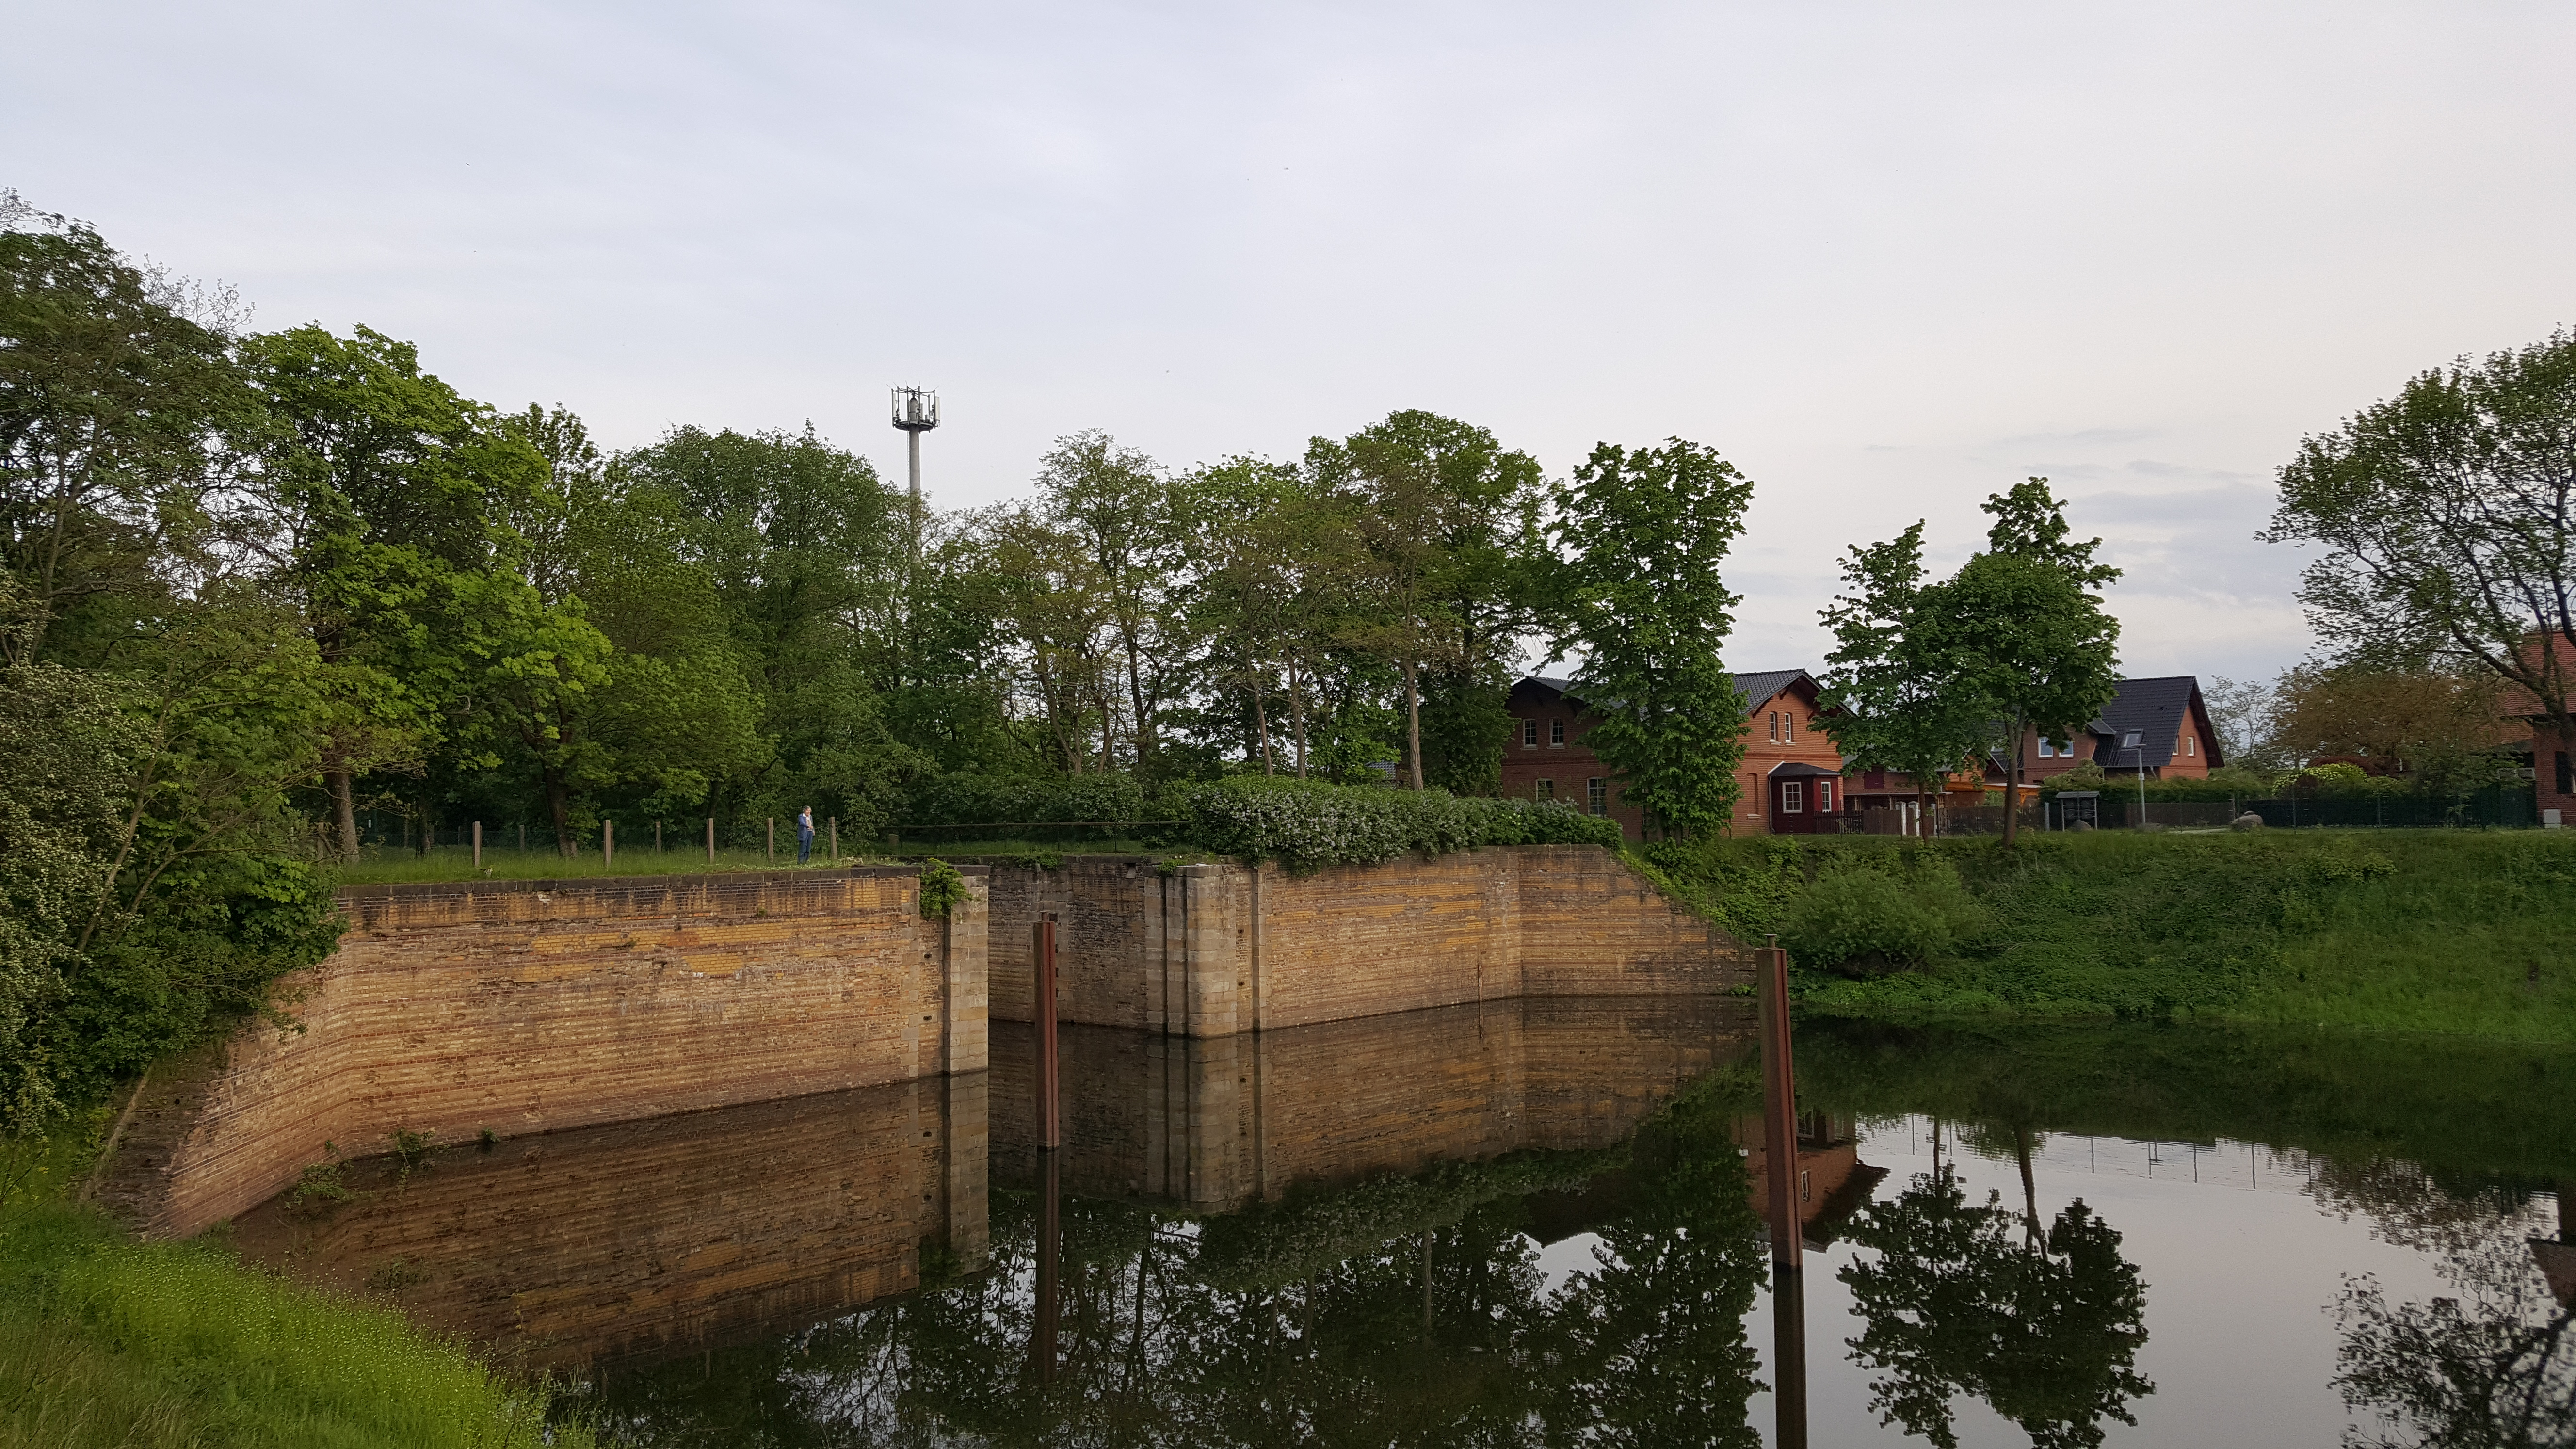
\includegraphics[width=\linewidth]{Photos/20210520_194728.jpg}}
	\caption{Alte Schleuse in Niegripp, Mai 2021}
	\label{fig:schleuse_niegripp}
\end{figure}

Der Schauplatz meiner Kindheit war Niegripp, da, wo der Ihlekanal in die Elbe mündet. Haus und Garten standen im Windschutz des hohen Elbedammes, der hier auslief in das Schleusenplateau, eine künstliche Aufschüttung mit den Häusern des Zolleinnehmers Wagner und des Schleusenmeister Zültz. Aus unserem Garten führte eine Treppe hinauf, und nach wenigen Schritten gelangte man zu einer stets nach frischem Brot und Bier riechenden Baracke, wo die Schiffer während oder vor dem Durchschleusen einkauften und sich erfrischten. Rechts davon ein großer Schuppen mit geteerten Balken, in dem es sich für Kinder bei Regenwetter herrlich saß. Am Schleusengehäuse und hinter unserem Garten führten zwei steile Steintreppen hinab zum Kanal. Dieses ganze Gelände war ein herrlicher Tummelplatz und wurde in meiner frühen Kindheit argwöhnisch vom Schleusenmeister Zültz und vom einarmigen Kanalaufseher Timmermann, einem Veteran des Krieges 1870/71, bewacht; in ihnen sah ich meine natürlichen Feinde, denn beide stellten ein fürchterliches Gebrüll an, wenn ich die Treppen zum Kanal hinab oder über den allerdings für Kinder nicht geschützten Schleusensteg gehen wollte.

Meine Mutter hatte hier viele unsichtbare Verbotstafeln errichtet, und ich beneidete manchmal meine Freunde Gustav und Otto Lüdde, die solche Verbote nicht zu kennen schienen. Denn die Erziehung des \enquote{Ungi} und der dreieinviertel Jahre jüngeren Ella lag wesentlich in den Händen meiner Mutter. Mein Vater, damals \enquote{Königlicher Hilfsförster} im Dienste der Hausfideikommisverwaltung der Hohenzollern, war ein tüchtiger Forstmann, leidenschaftlicher Jäger und Heger sowie erfolgreicher Imker. Er war wenig zu Haus, ich erlebte ihn aber täglich bei den Mahlzeiten, ausgenommen das Frühstück.

Wenn er nicht im Dienst oder auf Jagd war -- was beides praktisch ineinander überging oder zusammenfiel, sah ich ihn an seinem Fahrrade basteln oder in der Bienenhütte werken. Er hatte eine Art selbständiger Wasserleitung in den Bienenkörben konstruiert und, wie ich noch 1949 in Niegripp hörte, auf einer Imkerausstellung in Genthin vorgeführt; er hat auch in Burg bei Magdeburg gelegentlich Vorträge über Fragen der Imkerei gehalten.

Ich erinnere mich, wie er einmal von meiner Mutter, immer wieder aufs Blatt schauend, den Vortrag auf Probe sprach, während sie ihn gelegentlich mit stilistischen Verbeserungsvorschlägen unterbrach. Da mein Vater meine Freiheit weniger einschränkte, erschien mir in der Frühzeit meine Mutter als der strengere Elternteil. Da sich in ein - zwei Fällen, wohl im Alter zwischen 5 und 7 Jahren, gezeigt hatte, dass ich nicht, wie sie es wollte, jede Mahlzeit der Erwachsenen vertrug, erklärte sie, ich hätte einen \enquote{schwachen Magen} und bekam (daher), ich glaube mit Ella, Diätkost: außer Wild wenig Fleisch, keine Wurst, kein Weiß- und übliches Roggenbrot, nur Schrotbrot mit Apfelscheiben und ein Glas Milch zum Abendbrot. Wenn meine Mutter krank oder zu ihren Verwandten nach Österreich oder Ungarn verreist war, was in der Niegripp-Zeit wohl jedes Jahr vorkam, wurde ich von unserem langjährigen, tüchtigen, auch eigenwilligen Dienstmädchen durch interessantere Kost mit Roggenbrot und sogar warmem Abendbrot, das mir ausgezeichnet bekam, entschädigt. Mittags, vor dem Essen, schlich ich gern in der Küche herum, denn meine Mutter gab ihrem \enquote{Ungi} (wie ich mich selbst nannte) eine Keule von dem \enquote{Fan} d.h. Fleisch, und zwar von dem in der Pfanne gebratenen Wildgeflügel; besonders Wildentenkeulen schätzte ich sehr.

Übrigens behielt ich meine private Kindersprache, wie ich glaube, lange bei, wohl bis zum vollendeten 5. Lebensjahr, da meine Eltern im Gespräch mit mir sich ebenfalls vieler meiner Privatvokabeln bedienten. Das entsprach übrigens ganz dem Standpunkt der damaligen Alterstufen-Psychologie; noch William Stern, Philosophieprofessor in Breslau, später Hamburg, lehrte 1913, die Kindersprache sei ein ehrwürdiges Produkt kindlicher Sprachschöpfung, das frühzeitig zu unterdrücken kein Anlass bestehe. Ich kann mich nur noch an wenige Wörter erinnern wie Fau (Fleisch), Gridika (Zigarre), Zang (Zeitung).

Meine Schwester, die als Mädchen sehr früh eine \enquote{eigene} Sprache entwickelte, nannte sich selbst \enquote{Miedi} und mich den \enquote{Biedi}. Wenn wir zusammen spielten, redeten wir uns so an bis ich mit 6 Jahren in die Schule ging, und ich übernahm manche Ausdrucksformen Ellas, die ich jedoch vergessen habe. Mit 5 Jahren spätestens hatte ich die Kindersprache abgelegt und sprach Hochdeutsch, während meine Gespielen vorwiegend platt (niederdeutsch) redeten. Im 4. Lebensjahr brachte mir die bei uns mit dem Opa wohnende \enquote{Oka} (Großmutter mütterlicherseits) die Uhrzeit bei. Auf einem Schränkchen (Vertiko) im Wohnzimmer stehend betrachtete ich das Zifferblatt des Regulators und stellte fest: \enquote{Es ist bald 4 oder es ist 6 durch}; die Minuten konnte ich erst zwischen 5 und sechs Jahren bestimmen. In Anwesenheit von Gästen hob man mich auf das Vertiko und mein Können wurde bewundert, \enquote{was mir genehm war}.

Bei uns wohnten Mutters Eltern; er \enquote{der Opa} hatte ein verschuldetes Gut ererbt, es frühzeitig verkauft und war Gutsinspektor bei irgendeinem Magnaten gewesen. Seinen beiden Kindern konnte er für damalige Verhältnisse eine ausgezeichnete Ausbildung geben, meiner Mutter die Erziehung in der Herrnhuter Töchterschule Kleinwelka bei Bautzen (einem Internat) -- die entsprechende Jungenschule hatte einst Fürst Pückler-Muskau besucht. Ihr Bruder besuchte das Görlitzer Wilhelm-Gymnasium, studierte Jura und wurde angesehener Rechtsanwalt und \enquote{Justizrat} in Görlitz. Dessen Sohn Walter -- mein mir etwa gleichaltriger Vetter -- wurde ebenfalls Jurist und stieg 1934 als tüchtiger Finanzsachverständiger zum Generaldirektor der Hapag auf, deren Aktienmehrheit nach dem 1. Weltkrieg meines Wissens in amerikanischen Händen lag.

Opa ging viel mit mir spazieren und vermittelte mir u.a. landwirtschaftliche Kenntnisse. So lernte ich im Vorschulalter die jungen Saaten nach Roggen, Weizen, Hafer, Gerste unterscheiden, was ich später und heute nicht mehr konnte. Man amüsierte sich, wenn ich vor Erwachsenen, so auch vor dem späteren Lehrer und Kantor, naseweise Äußerungen über Fleiß bzw. Faulheit der Bauern, Ordnung und Unordnung etc. der Felder tat. Er erklärte, ich sei \enquote{wissbegierig} während er bei meiner Schwester -- zu Unrecht -- nur \enquote{Neugier} diagnostizierte. Ich war der Verzug meiner Großmutter, der \enquote{Oka}, deren letzte Worte übrigens \enquote{der Ungi} gewesen sein sollten. Beide Großeltern starben kurz hintereinander mit 70 Jahren an Lungenentzündung. Ich erinnere mich, dass eines Abends der Arzt aus Burg in seiner Droschke kam, nach den Untersuchungen bedauernd \enquote{beginnende Lungenentzündung} sagte, und darauf meine Mutter still weinte. Das war 1900 bzw. 1901 das medizinische Todesurteil, denn damals gab es noch kein wirksames Medikament gegen Lungenentzündung, eine Krankheit, die um 1900 noch zu den häufigsten Todesursachen zählte.

\label{para:kindheitserinnerungen}Zu meinen frühesten Kindheitserinnerungen zählen folgende: In meiner Kindheit fanden in und bei Niegripp mehrfach Manöver Magdeburger Truppenteile statt: Pioniere bauten eine Pontonbrücke über die Elbe, Ulanen\footnote{Ulanen sind eine mit Lanzen bewaffnete Gattung der Kavallerie} ritten auf dem ausgedehnten Elbanger Attacken z.B. gegen feuernde Artillerie. Die Eltern gingen mit ihren kleinen Kindern zur Elbe und über die Pontonbrücke nach Heinrichsberg, der Schulunterricht fiel aus, die Klassen gingen mit Kantor und Lehrer ebenfalls zur Elbe. Ich hatte das 3. Lebensjahr vollendet, als ein solches Manöver mit Ulanen und Artillerie stattfand. Es ertönten gewaltige Kanonenschläge, man sprach viel von den Ulanen. Am nächsten Tage gab es bei uns zum Mittagessen Rouladen -- ich verstand Ulanen, glaubte, wir essen die totgeschossenen Ulanen auf; es bedrückte mich, ich wagte aber nicht, die erlösende Frage an die Eltern zu richten. Ein Jahr später wusste ich wohl schon, dass die Kanonen zwar sehr laut donnern, aber nichts Böses anrichten. Ich hatte aber, wie alle Dorfkinder, große Angst vor Gewittern. Einmal, an einem heißen Sommertag, donnerte es unaufhörlich aus einer dunklen Wolkenwand jenseits des Kanals. Meine Mutter und das Dienstmädchen putzen im Garten Gemüse und pellten Erbsen aus. Ich hatte fürchterliche Angst und wollte ins Haus flüchten, sollte aber draußen bleiben. Ich war erst beruhigt, als der Schleusenmeister (natürlich auf Bitten meiner Mutter) mit lauter Stimme verkündete: \enquote{Das ist nur Kanonendonner!}

Meine Mutter erzog mich zum Gehorsam, bekämpfte jedoch mit unnachsichtiger Strenge die Lüge. Im Herbst lasen wir, die beiden Lüddes und ich, unter dem Nussbaum Walnüsse auf. Wir schlugen auch mehrere auf und aßen sie, ich auch, trotz strengen Verbots (wegen meines angeblich schwachen Magens). Meine Mutter musterte darauf misstrauisch meine Mundpartie und fragte: Fritz, hast du Nüsse gegessen? Aus Angst vor Strafe log ich: Nein! Sie rief meine Kumpanen herbei und fragte: \enquote{Habt ihr Nüsse gegessen?} \enquote{Ja}. \enquote{Hat Fritz Nüsse gegessen?} \enquote{Ja} Nun holte sie die Hundepeitsche, legte mich übers Knie und verdrosch mich, allerdings ohne besonders stark aufzudrücken. Den ganzen Tag über ließ sie mich spüren, dass ich mit der Lüge etwas sehr Verwerfliches getan hatte.

Lebhaft interessierte mich früh der Fischfang, vor allem das Angeln. Ich beneidete Erwachsene und größere Jungs, die ich im Kanal nahe der Schleuse hinter unserem Garten angeln sah. Mit meinem Freunde Gustav Lüdde zusammen hatte ich eine Angelrute gebastelt. Eines Tages eilte ich mit ihr über das Schleusentor und jenseits die Treppe herunter ans Kanalwasser. Als Köder hatte ich ein Brotklümpchen verwandt. Es biss kein Fisch an. Plötzlich brüllte mich von hinter über mir der einarmige Kanalaufseher mit schrecklicher Stimme an. Ich zog mit Schwung die Leine aus dem Wasser, der Angelhaken verfing sich im Regenschirm Timmermanns, dessen Gepolter wurde noch schlimmer; schließlich riss ich den Haken los und rannte, während sich ein warmer Strom über Bein und Hose ergoss, angsterfüllt nach Hause. Die wahrheitsgetreue Schilderung des Vorgangs und wohl auch das Komische meiner Situation bewahrten mich vor Strafe.

Im Sommer vor meinem Eintritt in die Schule starb Bismarck; ich erinnere mich sehr genau daran: 14 Tage lang läuteten von 12-13 Uhr mittags die Glocken. Erstmalig in meinem Leben, so glaube ich, ergriff mich ein Gefühl der Trauer, vor allem auch genährt durch Gespräche der Eltern. Der große Mann, dem wir alle so viel zu verdanken hatten, der nur an das Wohl unseres Landes dachte, und den der undankbare Kaiser fortgeschickt hatte, war tot. Sein Bild hing, außer einem großen Farbstich von Versailles \enquote{Vue générale, prise du bassin d'Appolon} und Photographien von Verwandten, im Wohnzimmer. Es wurde später durch eine schöne Farbreproduktion eines Bildes von Lenbach ersetzt. Den Farbstich von Schloss und Park Versailles hatten meine Großeltern mütterlicherseits von einer patriotischen Erbauungsreise nach Paris und Versailles (Spiegelsaal!) mitgebracht. Meine Eltern hatten in den 90-er Jahren eine Verlobungsreise zum Hermannsdenkmal im Teutoburger Wald gemacht.

Nach dem Eintritt in die Volksschule wurde ich mit des Lebens ganzem Jammer konfrontiert: der Rohrstock war wichtigstes Erziehungsinstrument. Er verging wohl keine Stunde, in der nicht einer von uns Jungen mit dem Stock unter jämmerlichem Geschrei verprügelt wurde. Lehrer Witte legte die Jungs über eine der vorderen Bänke oder ein Bein auf die Bank stützend über das Knie, wobei dann das Opfer oft schrie \enquote{ich falle} -- er darauf boshaft lachend erwiderte \enquote{nein, Bürschchen, ich halte dich fest!} Meine Eltern erfuhren vom Lehrer, dass ich weich veranlagt sei, da ich jedes Mal aus Mitleid mitweinte!

In der ersten Rechenstunde hatte ich einen großen Erfolg: ich konnte als Einziger der ca. 30 Schulanfänger bis 100 zählen. \enquote{Fritz, kannst du noch weiter zählen?} Ich bejahte stolz. \enquote{Einhundert, zweihundert, dreihundert.} Lehrer Witte lehnte dies jedoch kommentarlos zu meiner Enttäuschung ab.

Der tägliche ausgedehnte Religionsunterricht wurde wegen der damit verbundenen Hausaufgaben: Auswendiglernen langer alttestamentarischer Geschichten mit befremdlichen Namen wie Abraham, Melchisedek, Obadja etc. etc. und vieler Liederstrophen als lästig empfunden. Meine Mutter griff helfend ein: sie ging mit mir am windgeschützten Ihlekanal spazieren, sprach Sätze und Strophen vor und paukte sie mir ein. Im Religionsunterricht lernte ich u.a., dass es der liebe Gott besonders schätzt, wenn man ihm zu Ehren Lobgesänge anstimmt. Meine Mutter hatte mich zwar frühzeitig beten gelehrt, pflegte mit mir aber keine religiösen Gesänge. So hielt ich es für nötig, allein Gott den Herrn singend zu preisen, schämte mich aber vor meinen Eltern. So sang ich abends, gelegentlich auch morgens leise unter der Bettdecke.

Als ich acht Jahre alt war, kühlte sich mein bisher inniges Verhältnis mit dem lieben Gott plötzlich vorübergehend ab; das kam so: über dem Spiel hatte ich eine der Hausaufgaben ganz vergessen, nämlich drei Strophen eines Kirchenliedes auswendig zu lernen. Ich erschrak, als mir dies kurz vor dem Einschlafen einfiel. Faulheit und Vergessen wurden gleichermaßen mit dem Rohrstock geahndet. Da kam mir ein rettender Gedanke: in letzter Zeit waren die Eigenschaften Gottes herausgearbeitet worden, voran Allmächtigkeit und Allgüte. Ich wusste, dass Gott ein inbrünstiges Gebet erfüllt. So flehte ich ihn recht innig an, er möge machen, dass ich am nächsten Morgen beim Erwachen die befohlenen drei Strophen schön auswendig hersagen kann; ich versäumte auch nicht, mein inbrünstiges Gebet mit einem leisen Lobgesang des Herrn unter der Bettdecke zu beschließen -- und schlief vertrauensselig ein. Wie groß war meine Bestürzung und Enttäuschung beim Erwachen, dass mich der liebe Gott schmählich im Stich gelassen hatte und ich konnte nicht eine einzige Zeile hersagen. Das nahm ich ihm sehr übel und stellte für mehr als eine Woche Gebete und Lobgesänge ein.

Das alte Vertrauensverhältnis stellte sich erst später nach folgendem Vorfall wieder völlig her: im Herbst hatte ich eine Leiter an die mit Weinreben bedeckte Südwand des Forsthauses geschleppt; ich wollte mit meinem Taschenmesser ein paar Reben schneiden; oben stehend entglitt mir das Messer, ich suchte und suchte lange, im Wein, auf der Erde -- es war weg, nicht zu finden. Für einen Jungen damals ein sehr schmerzlicher Verlust! Ich richtete, noch auf der Leiter stehend, einen Hilferuf an Gott, und wiederholte mein Flehen im Abendgebet. Und siehe da! Am nächsten Morgen lag mein Messer auf dem Fensterbrett im Wohnzimmer! Ich war vom persönlichen Eingreifen Gottes überzeugt.

Im Sommer des wohl gleichen Jahres rauchte ich meine erste Zigarre. Die Eltern waren wie jeden Sonntag zur Kirche gegangen, das Mädchen arbeitete in der Küche, die Luft war rein; ich holte aus der eben angefangenen Kiste meines Vaters eine dicke Zigarre, nahm Streichhölzer, lief durch den Garten zur Böschung des Schleusenplateaus, schnitt wie der Vater die eine Spitze ab und zündete sie an, tat einige Züge, der Rauch kratzte scheußlich im Halse, so dass ich die brennende Zigarre ins Gras warf. Vater entdeckte alsbald die Lücke in der Kiste, sein Verdacht fiel sofort auf mich, ich gestand alles. Mein Vater schien eher belustigt als entrüstet.

Das wichtigste Spielzeug eines etwa 5-8 Jahre alten Dorfjungen war damals: im Frühjahr selbstgefertigte \enquote{Flitzbogen} mit Holzpfeilen, deren Enden einen aufgesetzten Kolben aus Holunder erhielten. Man fertigte Pfeifen aus saftigen Weidenruten, die mit dem Messerrücken weich geklopft wurden, so dass man das eingekerbte Holz aus der Rinde lösen konnte. Mit etwa acht Jahren spielte man mit einem großen Holzreifen, den man mit einem kurzen Holzstück schnell fortbewegte. Im März-April spielte der Holzkreisel eine Rolle; man schlug auf Fußwegen oder ebenen Fahrwegen auf ihn ein, man hatte gern zwei oder drei verschieden gefärbte Kreisel. Luxus waren schon summende Brummkreisel, Geschenke von Verwandten aus Berlin. Auch Spiele mit \enquote{Schnappkugeln} aus Glas oder gefärbtem Ton waren beliebt.

Ein großes Ereignis waren jedes Jahr die Sedanferien\footnote{der Sedantag war bis 1918 ein Feiertag anlässlich der entscheidenden Schlacht im Deutsch-Französischen Krieg 1870/71}. Eingeleitet wurden sie am Vorabend nach Einbruch der Dunkelheit durch Zapfenstreich. Voran die Dorfkapelle, gefolgt von der Bevölkerung und vor allem der Kinder mit Lampions; am schönsten war der Marsch auf dem Elbdamm und der Rundmarsch auf dem Schleusenplateau. Der Zug hielt vor dem Gutshaus, dem Pächter der zum königlichen Hausfideikommiss gehörenden Domäne der -- soweit eine solche vorhanden war -- die wichtigste Persönlichkeit des Dorfes war, nicht etwa Pastor oder Kantor. Er hielt die patriotische Ansprache mit dem Hoch auf Seine Majestät. Am nächsten Tag war schulfrei: Nachmittags und abends fanden auf dem Anger unter \enquote{den großen Eichen} Spiele für die Schulkinder statt, auch Blindekuh, Sackhüpfen und allerlei Wettspiele gehörten dazu. Die Kapelle spielte Märsche und Heimatlieder. Männer und Jugendliche drängten sich um eine Schießbude. Abends wurde im Saale des Gasthofs \enquote{Zum grünen Baum} getanzt.

Vor allem im Sommer lungerten wir Jungs viel an der Kanalschleuse herum und beobachteten den Dampferverkehr auf dem Kanal; wie die heutige Jugend jede Automarke kennt, so kannten wir die Namen der Dampfer, bevor sie mit eingeholtem Schornstein die Kanalbrücke passierten \enquote{Da kommt die Emma!} \enquote{Döskop; dat is doch die Schnakenburg.}

Den Verkehr auf der Elbe beobachteten wir vom Damm aus. Die großen Elbkähne, die oft in langen Schleppzügen von bis zu 22 Schiffen fuhren, zogen bei günstigem Winde ihre großen weißen Segel auf. Wir knüpften Bekanntschaften mit Schifferkindern der oft nur für wenige Stunden in Niegripp vor Anker gehenden Kähne an.

Ein großartiges Schauspiel war das nicht seltene Hochwasser der Elbe. Wenn das Wasser vormittags stieg, die Chaussee zum Fährhaus überflutete und sich rauschend in die tief gelegenen \enquote{Kolke} ergoss -- der \enquote{Heller} war nur 150~m von unserem Haus entfernt, der \enquote{Schweinebolk} 500~m -- fiel der Unterricht aus. Der Lehrer begab sich mit uns Schülern auf den Damm und dicht an die hereinbrechenden Fluten.

Hochwasser im Winter: Papa ließ im \enquote{Bauernbusch} Holz schlagen für Faschinen\footnote{Faschinen sind walzenförmige Reisig- bzw. Rutenbündeln von einigen Metern Länge, welche in erster Linie zur Abwehr von Erosionserscheinungen genutzt werden}. Unter seiner Leitung wurden die schwachen Stellen in Eile befestigt. Ich erinnere mich an eine unruhige Nacht, in der mein Vater verkündigte: Hochwasser um weitere 20 cm gestiegen und schließlich erlösend: 5 cm gefallen, Dammbruch bei Hohenwarte 7~km oberhalb Niegripp.

Im Winter tummelte man sich auf dem Eise -- mit 7 Jahren bekam ich Schlittschuhe. Bei hohem Schnee wurde ich in den ersten Schuljahren dicht vermummt auf einem Schlitten mit Rücklehne in die Schule gefahren, damit ich nicht kalte oder gar nasse Füße bekäme.

Im Winter 1900/1901 nahmen uns die Eltern zu einem 14-tägigen Aufenthalt in Berlin mit. Ich erinnere mich deutlich an die Bahnfahrt durch die tief verschneite Landschaft, an das rätselhafte Auf und Ab der Telegraphendrähte vor dem Abteilfenster und in Berlin natürlich vor allem an die vielen Pferdebahnen auf den Straßen und an die noch nicht so zahlreichen elektrischen Straßenbahnen, über denen an den Drähten so oft die bläulich blitzenden Funken sprühten. Ich soll oft \enquote{quengelich} und \enquote{unleidlich} gewesen sein, so besonders wenn wir mit einem Pferdevehikel fuhren, statt mit der Elektrischen. Mit einem Pferdevehikel fuhren wir ja schließlich auch von Niegripp nach unserer Kreisstadt Burg. Überwältigend war der Eindruck vom damals größten Warenhaus Berlins, Wertheim in der Leipziger Straße.

Einmal stand mein Vater mit mir vor der Berliner Haupt-Feuerwache. Bald ertönte ein schrilles Klingelzeichen, ein großes Tor öffnete sich, und heraus kam im Karacho die große von sechs Pferden gezogene Feuerspritze. Von den Verwandten, mit denen wir zusammen kamen, erinnere ich mich vor allem an Tante Martha Dehnicke, von Beruf Lehrerin, eine Cousine meiner Mutter, die erste Frau, die ich oft rauchen sah, was mir damals imponierte. Sie war überdies wegen ihrer erlesenen Geschenke, meist mit einem \enquote{Pfiff}, bei uns Kindern besonders gut angeschrieben. Später heiratete sie ihren Vetter Dr. Hans Dehnicke, nachmals Universitätsprofessor für Chemie an der Berliner Universität.

Im Sommer des gleichen Jahres, 1901, in dem mein Großvater Kurt Hoffmann, der mich oft auf seinen Spaziergängen mitgenommen hatte, gestorben war, hatte ich das Erlebnis der \enquote{ersten Liebe}. Sie hieß Anna Schmidt, war wie ich 8 Jahre alt, aus Magdeburg-Sudenburg und drei Ferienwochen zu Besuch in einem Nachbarhause. Wir fanden sofort aneinander Gefallen. Wir spielten täglich miteinander, trieben uns auf dem Anger herum, planschten im \enquote{Heller}, angelten zusammen. War ich mit Anna zusammen, störte mich die Anwesenheit meiner Niegripper Spielgefährten, einschließlich meiner Schwester Ella. Ich erfand Vorwände, um die anderen Jungen von uns fernzuhalten. Wir wussten einander stets viel zu erzählen. Mich interessierte Annas Leben und Magdeburg. Schließlich kam der Abschied. Er fiel uns schwer. Anna fuhr mit dem kleinen Dampfer, mit dem sie gekommen, eines Vormittags wieder zurück nach Magdeburg. Ich stand lange an dem Buhnenkopf, an dem der Dampfer angelegt hatte, und winkte und winkte, bis das Schiffchen zu einem Punkt mit einer schwachen Rauchfahne darüber zusammengeschrumpft war. Meine traurige Stimmung hielt mehrere Tage an. Nach einigen Wochen kam aus Sudenburg eine mit ungeübter Kinderhand geschriebene Karte, deren Inhalt ich wieder und immer wieder las: \enquote{Denkst du auch noch an mich? Ich denke aber an Dich. Deine Anna Schmidt}. Ich habe sie nie wieder gesehen.

Im gleichen Sommer, etwas später, verbrachten zwei Verwandte Kurt und Wilhelm Bertling aus Aachen ihre Ferien beim kinderlosen Ehepaar Wagner, Schleusenzoll Einnehmer wohnhaft auf dem Schleusenplateau, zwei nette mit mir gleich bzw. zwei Jahre ältere Jungen. Lebhafte, gepflegte Großstadtjungen, denen ich manche Anregung verdankte. Beide trugen schöne baumwollene Spielanzüge und Sandalen. Meine Mutter ließ mich im Sommer barfuß laufen (\enquote{das ist gesünder}), auf meine Kleidung verwandte sie geringe Sorgfalt (ich hatte einen \enquote{Paradeanzug} für Sonn- und Festtage, den ich hasste, da ich praktisch in ihm nicht frei spielen konnte.)

In der Gegenwart der Bertling-Jungen fühlte ich mich wegen der modernen Bekleidung frustriert. Mein Vater erklärte mir zwar, die Bertling-Jungen kämen von weither, von der Reichsgrenze, aber hier, unweit Berlins, der Residenz des Kaisers, könne man nicht so gekleidet gehen -- doch das überzeugte mich nicht. Einmal, als ich barfuß in Hemd und Hose im Garten spielte und plötzlich die beiden Bertlings schick angezogen die Treppe vom Schleusenplateau heruntersteigen sah, kam es zu einer Kurzschlusshandlung: ich rannte, was hast du -- was kannst du, fort und versteckte mich in einer Kartoffelfurche, wurde aber dort entdeckt und schämte mich -- zum Erstaunen der Bertling-Jungen.

Ein anderes Mal hörte ich von Wagners, Kurt Bertling sei mit dem Dampfer \enquote{Gustav} nach Burg gefahren, musste aber bald zurückkommen. Ich ging am Kanal entlang bis zur ersten Brücke, sah \enquote{Gustav} kommen, Kurt am Bug stehen, rannte runter zum Fußgängersteg unter der Brücke und winkte in der festen Erwartung, der Dampfer würde anlegen und mich aufnehmen -- aber Enttäuschung, der Dampfer fuhr in voller Fahrt an mir vorbei, Kurt winkte mir vergnügt zu -- und ich versteckte mich schmollend irgendwo in den Büschen am Kanal, sodass mich Kurt an diesem Tag nicht mehr sehen konnte. Ich fühlte mich frustriert, gekränkt!

Einmal spielte ich mit Ella an der Elbe jenseits der Elbschleuse. Wir wurden von einem aufziehenden Gewitter überrascht und rannten beide, ich immer voran, auf den für Kinder nicht ungefährlichen Schleusensteg zu; ich rannte als erster herüber ohne mich um meine ein paar Pferdelängen mir folgende Schwester zu kümmern. Da donnerte mich die Stimme des Schleusenmeisters Zülz an: \enquote{Kerl, wirst du dich wohl um dein Schwesterchen kümmern?} Ich schämte mich, aber dieser Anranzer eines \enquote{Fremden} blieb nicht ohne positive Wirkung.

Besonders im Winter wurde Ella für mich zur wichtigsten Spielkameradin, da sie stets zur Stelle und überdies ein flinkes, einfallsreiches und gelehriges Mädel war. Zum 4. Geburtstag hatte sie auf ihren Wunsch eine Kiepe bekommen, wie die Niegripper Frauen sie auf dem Rücken trugen. Ein paar Tage drauf kam sie triumphierend vom Kolonialwarenhändler mit einer Tüte Bonbons in der Kiepe wieder -- mit Bonbons wurden wir von unserer Mutter sehr knapp gehalten. \enquote{Ja, woher hast du denn das Geld gehabt?} \enquote{Gar nicht. Ich hab gesagt: ich möchte für 10 Pfennig Bonbons aber ohne Geld!} Dieses Verfahren belustigte uns alle und imponierte mir. Ich las ihr gelegentlich Märchen vor, ging von Grimms Märchen bald zu \enquote{Tausend und eine Nacht} über, deren Phantasiereichtum mich mehr fesselten als Grimms Hausmärchen.

Wir spielten mit dem von Großmutter überkommenen Bildzusammensetzbaukasten und ich brachte ihr auch Dame und Mühle bei. Zum Damespiel stellte ich drei Stühle nebeneinander, auf den mittleren Stuhl kam das Damebrett -- denn in dieser Stellung spielte der von mir geliebte Hassan von Basra und die Prinzessin auf einem schönen bunten Bilde in \enquote{Tausend und eine Nacht} Schach! Ich verriet aber weder Ella noch meinen Eltern, warum ich gerade diese Stellung beim Spiel für richtig hielt.

Zu meinem 9. Geburtstag erhielt ich einen etwa 80 cm hohen Holzreifen, den man, neben ihm herlaufend, mit einem Stöckchen vorantrieb. Wir fuhren stundenlang auf Elbdamm und Radfahrstegen; in den Kurven zeigte sich der Geschicklichkeitsgrad. Im Winter freute ich mich schon auf den März als Wiederbeginn des Reifenschlagens -- doch zu diesem Zeitpunkt interessierte mich der Reifen nicht mehr -- warum? wurde mir damals selbst zum Problem -- und an seine Stelle trat der Kreisel.

Als ich neun Jahre geworden war, übersprang ich eine Klasse und kam in die Oberstufe des nüchternen, streng-gerechten Kantors August Kersten. Die großen Jungen hänselten mich anfänglich, z.B. \enquote{Fritz, wat sechste'n, wenn der Kanter euch besuchen kommt?} \enquote{Nu, gut'n Tach, Herr Kanter.} \enquote{Quatsch! Du sechst: Kanter, Küster, Organist -- siehste Aujust waste bist!} Neben meinem Sitzplatz war an die Wand gekritzelt zu lesen: \enquote{Was der Fleischer hackt, das wird wieder ausgekackt.} Die Richtigkeit dieses Satzes verblüffte mich.

Aber das Leben war etwas ernster geworden, ich hatte manches nachzuholen, und es war für mich nicht leicht, mich unter den größeren und durchweg älteren Jungen zu behaupten. Im Unterricht wurden gute bzw. schlechte Leistungen dadurch quittiert, dass man einen oder mehrere Plätze \enquote{herauf} oder \enquote{herunter} kam. Die guten Schüler saßen hinten, \enquote{herauf} hieß nach rechts rücken; man zog sofort mit Mappe und Büchern um.

Ostern 1903 bestand ich die Aufnahmeprüfung für die Sexta des humanistischen Victoria-Gymnasiums in Burg. Ich kam in Pension zu der mit meinen Eltern befreundeten Lehrerfamilie Seehaus, die in den Ferien bei ihrer Mutter Block in Niegripp wohnten. Ich schlief zusammen mit Paul, dem Untertertianer, spielte oft mit der gleichaltrigen Grete. Sonnabends fuhr ich nachmittags in der Regel mit der Postkutsche des Schlüter nach Hause; Montag früh um halb 7 Uhr nach Burg zurück, gelegentlich im Sommer mit dem Dampfer, der sonntags zwischen Burg und Niegripp auf dem Ihle-Kanal verkehrte. Ich erinnere an einen herrlichen Montagmorgen im Monat Mai, die Maikäfer umschwirrten die blühenden Pflaumenbäume längs der Chaussee; wie schade, dass die Kusche nicht anhielt!

Das Viktoria-Gymnasium war ein relativ moderner roter Ziegelbau aus dem letzten Drittel des neunzehnten Jahrhunderts. In ehrfurchtsvollem Ton wurde erzählt, dass bei der Einweihung Prinzessin X des kaiserlichen Hauses zugegen gewesen sei! Leiter des Gymnasiums war Gymnasialdirektor Passow, großer Propagandaredner im Flottenverein. In jeder Klasse hing eine große Karte mit graphischer Darstellung des Wachstums der deutschen im Vergleich zur englischen Flotte. So war unserem tüchtigen Direktor die für seinen Rang ziemlich seltene Auszeichnung des Roten Adlerordens III. Classe zuteil geworden! An Kaisers Geburtstag -- 27. Januar -- erschien er wie auch mehrere Lehrer in der prächtigen Galauniform des Reserveoffiziers. Die Disziplin am Gymnasium schien mustergültig zu sein. Unser Ordinarius (mit 8 Wochenstunden Latein) war Oberlehrer Seegers aus Buxtehude; er war streng, machte aber vom Rohrstock nur maßvoll Gebrauch.

Rechnen erteilte ein 73-jähriger Veteran aus dem Kriege 1870/71, dem ein Granatsplitter die Nasenspitze arg entstellt hatte. Er musste uns mehrere Male im Unterricht den Hergang erzählen. \enquote{Nanu, hab ich euch noch nicht erzählt wie ich verwundet wurde?} Wir logen: \enquote{Nein, Herr Oberlehrer}. -- \enquote{Also, es war bei Vionville, von dieser großen Schlacht werdet ihr schon gehört haben...} Wir kannten die Story schon fast auswendig.

Ich fand den Unterricht in wohl allen Fächern interessanter als in der Niegripper Volksschule und hatte keinerlei Schwierigkeiten. Der Besuch eines Gymnasiums kostete damals erhebliches Schulgeld, dazu kamen noch die Kosten der Schulbücher. \enquote{Hilfsbüchereien} gab es vor dem 1. Weltkriege nicht. So waren die \enquote{Gymnasiasten} in der weitaus überwiegenden Mehrzahl Söhne des wirtschaftlich gutgestellten Bürgertums.

Eine Unsitte der Sexta war die \enquote{Klassenkeile}, in den Pausen geduldet von dem aufsichtshabenden Lehrer und vollzogen an Schülern, die \enquote{gepetzt} hatten, was wohl nur zwei -- oder dreimal in der Sexta passierte, und am Geburtstag eines jeden. Man zog ihn über einen der Barren im Schulhof und jedes Mitglied der Klasse versetzte dem armen Opfer einen kräftig ausgeholten Schlag mit der Handfläche aufs Gesäß.

Im Schuljahr 1903/04 brach der russisch-japanische Krieg aus. Eine ganze Reihe von uns Sextanern, zu denen auch ich gehörte, interessierte sich lebhaft für das Kriegsgeschehen. Oft berichtete Herr Seehaus bei Tisch darüber, ich las auch die Berichte des \enquote{Burger Anzeigers}. Wir freuten uns, wenn \enquote{die Russen Kloppe kriegten}. Warum ich den Russen Niederlagen gönnte, weiß ich nicht, es war wohl so die allgemeine Volksstimmung. Einmal, in einer Zirkusvorführung, zwischen zwei Nummern, blieb ein schlecht gekleideter Mann in der Mitte des Zeltes stehen. Ein Clown trat auf ihn zu und redete ihn ohne jeden Erfolg in mehreren Sprachen an. Als er aber zum Schluss sagte: \enquote{Russe, die Japaner kommen}, rannte der Mann in panischer Angst davon -- und das ganze Publikum, jung und alt, jubelte.

Gegen Ende der großen Ferien führte mich mein Vater auf mein Drängen in das \enquote{Schießen mit einer richtigen Flinte} ein. Ich lernte die Flinte fest einsetzen, beim Abdrücken nicht \enquote{Mucken}, spürte beim Schuss den \enquote{Rückschlag}, sah zunächst das Ziel vor Pulverdampf nicht und durfte schließlich nach einigen Probeschüssen einen Neuntöter erlegen. Das genügte, um nach dem Wiederbeginn der Schule mit Erfolg vor den Klassenkameraden angeben zu können, die ihrerseits schon vielfach vor den Ferien mit ihrer bevorstehenden Reise \enquote{an die See}, \enquote{ins Riesengebirge}, \enquote{in den Thüringer Wald}, \enquote{den Spreewald} usw. angegeben hatten. Meine Eltern hatten zwar schon mehrfach mit Freunden Wochenendfahrten in den Harz unternommen, uns Kinder jedoch stets unter der Obhut unseres langjährigen Hausmädchens Marie Tucher zurückgelassen. Manche Klassenkameraden beneideten mich nun offensichtlich, dass ich schon mit einem \enquote{richtigen Gewehr} (und nicht bloß mit einer Luftbüchse) geschossen und sogar einen Vogel erlegt hatte! Mein Ziel hatte ich damit erreicht.

Zu dieser Zeit fertigte ich auf zwei Sitzungen auf dem Klo -- dem einzigen Ort, wo ich bei Seehauses allein war -- ein zweistrophiges Gedicht über das Wetter an. Ich zeigte es dem Untertertianer Paul Seehaus, einem Musterschüler; der las es mit Stirnrunzeln und meinte dann: \enquote{da denkst du wohl, ich glaub dir, dass du das gemacht hast?! Das hast du einem Lesebuch abgeschrieben} Jeder Widerspruch erwies sich als erfolglos. Ich war betrübt aber innerlich doch ein wenig stolz, dass ein so großer Junge mein Produkt implizit lesebuchreif hielt!

Einmal im Frühjahr und einmal im Herbst verkündete Herr Seehaus: Vater Busse steht heute im Kreisblatt! Da konnte ich lesen, mein Vater hatte im \enquote{Hotel zum Schulterblatt} einen Vortrag über ein Jagdthema gehalten; das andere Mal handelte es sich um eine Imkertagung in Genthin, wo er das Modell eines Bienenkorbes mit von ihm erfundener automatischer Wasserleitung vorführte.

Meine Niegripper Schulfreunde traten nach dem Schulwechsel allmählich etwas in den Hintergrund. Am Wochenende und in den Ferien spielte ich mehr mit Ella, für deren Puppenstube ich vor Weihnachten von meinem Taschengeld verschiedene Gegenstände, unter anderen auch einen Nachttisch mit zierlichem Porzellantöpfchen zusammenkaufte, was die Kritik meiner Pensionseltern herausforderte.

Zum 1. April 1904 wurde mein Vater nach Niederschlesien versetzt; er erhielt die Revierförsterei Karlshof bei Tschirne Kreis Bunzlau mit dem Revier Karlshof, Siegersdorf und dem 20~km entfernten Thomaswaldau. Sie war 4,5~km vom nächsten Bahnhof Siegersdorf und dieser 14~km von Bunzlau entfernt. Zur Försterei gehörten 40 Morgen Ackerland und Wiese, die mein Vater verpachtete. Unsere Familie zog nach Neujahr mit Marie Tuchen um, während ich noch bis zum Beginn der Osterferien in Burg blieb.

Herrlich war das Schlittschuhlaufen im Januar und Februar. Zur letzten Lateinstunde -- dafür gab es immer die meisten Hausaufgaben auf -- hatte ich die aufgegebenen Vokabeln nicht mehr gelernt, fiel prompt herein und zog mir ein missbilligendes Kopfschütteln des Oberlehrers Seegers zu mit den Worten: \enquote{Busse, das ist nicht schön!} Die bekannte Auflockerung des Unterrichtsbetriebes am letzten Schultage mit Vorlesen u.ä. kannte man damals noch nicht.

Und nun war auch der Tag gekommen, an dem mein Vater mich abholte; er hatte auf dem Burger Güterbahnhof noch viel mit der Vertrimmung seiner 30 großen, sehr modernen Bienenkörbe zu tun. Dann führten uns 7 Schnellzugstunden über Kohlfurt nach Siegersdorf.


\marginpar{38}
\section{Siegersdorf bei Bunzlau}
Frau Nietschke holte uns mit einem großen Handwagen für das Gepäck ab. Sie sprach schlesische Mundart, sodass ich sie nicht verstand. \enquote{Nu gieste wull eia Bunzel?}\footnote{Nun gehst Du wohl nach Bunzlau?} Diese Frage übersetzte mir erst meine Mutter ins Hochdeutsche. Der Weg führte etwa 2~km durch den Forst meines Vaters, Kiefernwald mit viel -- mir neu -- Blaubeer- und Preisselbeerkräutern; dann schritten wir durch das langgestreckte Dorf Tschirne, über den gleichnamigen Bach, leicht ansteigend über Wiesen und Ackerland zum Karlshof, gelegen am Rande einer Schonung, dahinter ca. 30-jähriger Wald, weiter Blick über Tschirne bis zu den Silhouetten des Isar- und Riesengebirges; einsam, das nächste Gehöft von Tschirne über 1~km entfernt. Dass wir auf einer Wasserscheide wohnten, war möglicherweise der Grund für die vielen sehr heftigen und anhaltenden Gewitter, die wir erleben sollten.

Unserer langjährigen Hausangestellten war es zu einsam, die Schlesier in Sprache und Wesen zu ungewohnt; sie verließ uns nach ein paar Monaten. Ihre Nachfolgerin blieb auch nicht lange, sie schrieb ihren Eltern: es donnert hier Tag und Nacht, ich fürchte mich so (sprich: firrt). Wir beiden Geschwister spielten viel mit den beiden mittleren Kindern des Tschirner Pastors Brückner, Martin und Dora, beide 1-2 Jahre älter als wir. Mit Martin, der in die Quarta aufgenommen wurde, kam ich in die Pension des weißhaarigen emeritierten Kantors Kattein, wo wir mit drei etwa gleichaltrigen Jungs in der gleichen Stube wohnten. Gleich nach dem Mittagessen wurden die Schularbeiten gemacht, dann ging's hinaus, im Frühjahr \enquote{schackten} wir nach dem 5~km entfernten alten Sandsteinbruch von Altwarthau, wo wir an einer Höhle buddelten, verfolgt von einem imaginären Räuber, der uns nach dem Leben trachtete; zu unserer Verteidigung führten wir Lederriemen mit uns. Die 5~km zurück wurden ebenfalls \enquote{geschackt} (gerannt im Dauerlauf).

Im Frühsommer und nach den großen Ferien tummelten wir uns im Bober. Beim Fischer Konetzke holte ich mir immer für 10 Pfg. für den ganzen Nachmittag das Ruderboot Toni, dann ging es zu einer Sandbank gegenüber einem tiefen Strudel \enquote{Teufelsküche}, in dem zwei Jahre später einer meiner Klassenkameraden ertrank. Wir lieferten uns auch \enquote{Seeschlachten}, indem wir mit den Rudern (wir sagten Pötschen) aufeinander einschlugen, bis uns der Fischer auseinanderjagte.

Es war ein heißer, trockener Sommer. In den großen Ferien konnten wir vom oberen Ostzimmer des Forsthauses in der Ferne ab und zu weiße Rauchsäulen beobachten -- Waldbrände! Bald machte sich eine große Raupenplage gemerkbar: die Nonne fraß erhebliche Teile des Karlshofer Kiefernwaldes kahl. Der niederfallende Raupenkot verursachte das Geräusch wie von einem sanften Regen. Mein Vater ließ zum Schutze der 10-jährigen Schonung zwischen dem Forsthaus und dem Wald kleine 30 cm tiefe Gräben mit steilen Wänden ziehen, die von den Nonnenraupen in der Regel nicht überwunden werden konnten und in denen sie auf der Suche nach noch benadelten Kiefern zu Tausenden umkamen.

Zwei Tage nach Schulbeginn am 6. August 1904 wurden wir Jungs durch Sturmläuten vom hohen Turm der evangelischen Kirche, unter dem die Katteinsche Pension lag, um 5 Uhr früh geweckt. Wie sich herausstellte war der Anlass ein Großwaldbrand bei Primbenau, verursacht durch Lokomotivfunkenflug der Strecke Glogau-Liegnitz, dessen die Feuerwehren und bereits eingesetztes Militär der benachbarten Ortschaften und Kleinstädte nicht hatten Herr werden können. Vom über 40~m hohen Turm des Bunzlauer Gymnasiums sahen wir fern -- ca. 36~km entfernt! -- eine breite weißliche Rauchfläche am Horizont. \num{23000} Morgen Waldes, ein paar Menschen, vom Feuer eingeschlossene Gehöfte und viele Rehe und Hirsche fielen dem Flammen zum Opfer. Wie ich von meinem Vater hörte, war der Brand streckenweise durch Anlage eines Gegenfeuers mit Erfolg bekämpft worden.

Inzwischen hatte ich mich längst in Bunzlau eingewöhnt. Klassenleiter Dr. Thoma, Typus des strammen Reserveoffiziers, gab straffen Unterricht; leider arbeitete er zuviel und rücksichtslos mit dem Rohrstock. Bei mangelndem Fleiß gab es zunächst heftige Schläge auf die Hand, im Wiederholungsfalle legte er sein Opfer über die Bank und verdrasch [sic!] es jämmerlich. Zweifellos -- man lernte etwas bei ihm. Neben Latein und Deutsch erteilte er auch den Erdkundeunterricht, damals kaum mehr als Topographie Deutschlands. Wiederholungsfragen z.B.: Wo liegt Bonn? (am Rhein) Wieweit von welcher Großstadt entfernt? (Köln, 35~km Was weißt du noch von Bonn? (In Bonn studieren die Herren \enquote{von}) Wo liegt Jena? (an der Saale) Was weißt du noch von Jena? (Universität: in Jene lebt's sich bene) Wo wächst in Deutschland Hopfen? (Maingegend) Warum ist Hopfen wichtig? (Hopfen und Malz, Gott erhalt's!) Das mussten wir herungerschnurren. Nachmittags sahen wir ihn gelegentlich mit Monokel spazierengehen. Montag früh war er stets schlechter Laune, besonders wenn er die wöchentlich fällige lateinische Klassenarbeit zurückgab. Grobe Fehler kennzeichnete er durch ein nb; das hieß praktisch, dass man sich melden musste, die Hand ausstreckte und er nach kurzer Erklärung des Fehlers einem die richtige Form mit Stockschlägen auf den Handteller eingebläut wurde.

Besonders schlecht zu sprechen war er auf den Adel in der Klasse, der ihn vielleicht durch eine aristokratisch nonchalante Art reizte. Dann rief er: \enquote{Von Bönigk, von Zühlow, von Fauck -- raus! Euer Deputat!} Und verdrasch ihnen den Hintern.

\enquote{Schönschreiben} hatten wir zweimal wöchentlich bei einem alten massigen Volksschullehrer, dessen Bewegungen langsam und dessen Sprache tief und bedächtig war. Wir nannten ihn \enquote{Bulle} und bewarfen ihn gern mit Papierkugeln. Er sagte oft: \enquote{Wenn ich aber mal einen von euch erwische, der kann sich auf was gefasst machen}. Einmal drehte er sich schneller als gewöhnlich zur Klasse um, da traf ihn mein Papierball mitten ins Gesicht. Er erblickte meinen noch ausgestreckten Arm und rief: \enquote{Busse, raus!} Er packte mich am Kragen, schleppte mich ins Konferenz-Zimmer und holte aus einem Schrank einen langen Rohrstock heraus. Ich bat weinerlich: \enquote{Herr Lehrer, ich will's ja nicht wieder tun\dots} Er triumphierend darauf: \enquote{Ja, Bürschchen, das will ich dir glauben.}, und dann verdrasch er mich.

Im Winterhalbjahr setzte verstärkt das Sammeln ein, wir Jungs sammelten Bilder, Beigaben vom Stollwerk-Automaten u.ä., fingen auch schon an, Briefmarken zu sammeln.

Das Weihnachtsfest im Elternhaus war natürlich der Höhepunkt des Winters. Es fand seinen Abschluss mit dem sogenannten Plündern des Weihnachtsbaumes zu Neujahr, d.h. des Abnehmens der zahllosen am Baum hängenden \enquote{Ringel}-Süßigkeiten aller Art, die zwischen Ella und mir geteilt wurden. Ich bewahrte meinen Anteil sorgfältig verpackt in einer Kiste in einer Dachkammer auf. Als ich knapp 14 Tage nach Neujahr zum ersten Mal im neuen Jahr am Sonnabend wieder nach Hause kam und sogleich meine Kiste aufsuchte -- war sie leer, kein einziger Ringel mehr drin. Ella, diese Missetäterin, hatte alle aufgegessen. Meine Eltern hatten alle Mühe, meinen Zorn zu besänftigen.

Schön war auch der Winter in Bunzlau, Eislaufen auf dem Schlossteich und Rodeln in der Zeche. In der Zeit des Wintersports waren meine Leistungen in verschiedenen Fächern rückläufig; im März holte ich aber auf.

In Quarta -- Ostern 1905 -- waren wir 44 Schüler, deren fast 1/3 Sitzenbleiber waren; auch mein Dorfkamerad Martin Brückner war sitzengeblieben und ging nach Görlitz (Realgymnasium) ab. Sitzengeblieben war auch der Pastorenjunge Hans Menzel, der dann in meiner Klasse bis zum Abitur verblieb. Leider saß ich -- als einer der ersten versetzt -- in der großen Klasse hinten und war daher oft abgelenkt. Unser Klassenleiter Prof. Altmann schien mir weder ein guter disziplinierter Lehrer noch kenntnisreich zu sein. Mangelnder Fleiß und Aufmerksamkeit sowie Vergesslichkeit bestrafte er mit rasch erteilten, wohlgezielten Ohrfeigen, auch noch in Untertertia. \marginpar{47} Wir nannten ihn \enquote{Damlich}; man sagte von ihm -- er war Raucher -- dass er zu Hause vor dem offenen Ofentürchen sitze und den Zigarrenrauch auf Befehl \enquote{seiner Alten} hineinblasen müsse, damit die Gardinen nicht grau würden\dots

Rechnen hatten wir bei einem Oberlehrer Hähnel, der bei der Rückgabe der Klassenarbeitshefte folgende Prädikate verlas: gut (sehr gut kam meines Wissens nicht vor), genügend, wichse! (mangelhaft), buh! (ungenügend). Er verdrasch die Urheber mangelhafter Arbeiten weil er glaubte, sie auf diese drastische Weise zu genügenden Leistungen anspornen zu können; Verfasser ungenügender Arbeiten hielt er für \enquote{buh} = verrückt, geistig minderwertig, die er links liegen ließ.

Musikunterricht, \enquote{Singen} genannt, fiel ab Quarta fort; es gab nur nachmittägliches \enquote{Chorsingen}, für das die Schüler in einer kurzen Prüfung durch Prof. Heyse ausgesucht wurden. Er schlug einen Ton auf dem Flügel an, ich sang absichtlich ein bis zwei Töne tiefer. Das wiederholte sich noch zweimal, dann rief er: \enquote{Weg; untauglich!} Der Grund meiner geheuchelten Unmusikalität war die Angst, mir durch zweimaliges Chorsingen in jeder Woche zwei schöne Spielnachmittage zu verderben. Später habe ich das bereut, wie ich auch bereut habe, dass ich den Klavierunterricht, den mir meine Mutter im Sommer 1904 an Wochenenden und in den Ferien erteilte, schließlich sabotierte, weil mir das Üben keinen Spaß machte. Leider konnte sie, die eine sehr gute Klavierspielerin war und fast jedes Jahr einem oder zwei Kindern von Pastoren, Post-, Bahn- und Fabrikbeamten aus Siegersdorf Unterricht erteilte, sich mir gegenüber nicht durchsetzen. Umso mehr Erfolg hatte sie mit meiner Schwester; jedem Besucher wurde eine vierhändig gespielte musikalische Begrüßung geboten. Sie liebte besonders Beethoven. Ella lernte später auch noch Gitarre und Akkordeon spielen.

Neu trat im Lehrplan der Quarta Französisch mit vier Wochenstunden, ab Untertertia bis zum Abi jedoch mit nur zwei Wochenstunden und fungierte nur als Nebenfach neben den Hauptfächern Latein-Geschichte-Deutsch-Mathematik. Nur auf diese Fächer erstreckte sich auch die schriftliche Reifeprüfung. Der Französischunterricht blieb im bloßen Grammatik- und Übersetzungsunterricht an Hand des alten Plock stecken. Mündliche oder schriftliche Nacherzählungen betrieb man nicht. Sprechübungen blieben auch auf der Oberstufe in dürftigen Anfängen stecken, obwohl wir den Fachlehrer baten, im Unterricht mit uns französisch zu sprechen; die beiden Fachlehrer für Französisch beherrschten die gesprochene Sprache nur unzulänglich. Meine Mutter, die ebenso wie meine Großmutter auf der Herrenhuter Schule Bautzen bzw. Kleinwelka bei Bautzen einen für das 19. Jahrhundert guten französischen und englischen Unterricht genossen hatte, überwachte während der ganzen Quarta meine Leistungen in Französisch und \enquote{nahm mich} zu meinem Leidwesen meistens Sonntagvormittag im Französischen \enquote{vor}. Das hatte zur Folge, dass ich ab Quarta dank der festen Grundlage und des geweckten Interesses bis zum Abi in Französisch der Klassenbeste war.

Meine Mutter erteilte gelegentlich einzelnen Kindern und Erwachsenen neusprachlichen Unterricht unter Zugrundelegung ihrer Schulbücher; französische oder englische Literatur hatte sie nicht gelesen, war auch nie im westlichen Ausland, während sie in meiner Kindheit mehrfach zwei, drei Wochen zu ihren Verwandten in Böhmen (Mariaschein bei Teplitz) und Prag, Budapest und Fünfkirchen reiste. Immerhin erzählte mir 1914 ein gebildetes Mädchen aus La Chaud-de-Fond (Westschweiz), die ein paar Monate bei der mit uns befreundeten Nachbarsfamilie Dr. med. Thumne (dessen Frau eine Tochter des Geh. Rates Steinberg und Schwester der Lotte Steinberg war) zur Pflege der französischen Konversation verbrachte, sie sei, als sie meine Eltern das erste Mal besuchte, von meiner Mutter mit mehreren völlig korrekten französischen Sätzen begrüßt worden, beginnend mit: soyez la bienvenue dans ma maison\dots

Sommers und Winters, schon in Quinta beginnend, vor allem aber als Quartaner und Untertertianer prügelte sich unsere Pension bzw. Stube oft mit den \enquote{Kläppern}, etwa gleichaltrigen Volksschülern, so genannt wegen der klappernden Holzpantoffeln, die damals statt Schuhen von den ärmeren Kindern getragen wurden. Bei Verfolgungen nahm man die Pantoffeln in die Hand und machte sich \enquote{auf die Socken}. Wir fühlten uns provoziert, wenn die \enquote{Kläpper} uns auf der Straße nachriefen: \enquote{Gymnasiasten scheißen in'n Kasten} und stürzten uns auf sie mit dem Rufe: \enquote{Ihr verdammten Kläpper!} Als ich eines Sonntags wie gewöhnlich Rucksack auf dem Rücken, nach 19 Uhr mit dem Siegersdorfer Zuge vonhause zurückkehrend auf der \enquote{Promenade} zur Pension schlenderte, überfielen mich plötzlich aus dem Gebüsch heraus zwei \enquote{Klepper}, einer von vorn, der andere von hinten, rissen mich zu Boden, schlugen mich ins Gesicht und entwichen in der Abenddämmerung. Ich kam, aus einer Kratzwunde im Gesicht blutend, zum Abendessen, wo mein Fall Aufsehen erregte. Anschließend trat die Stube zum Kriegsrat zusammen: für den folgenden Nachmittag wurde ein Rachefeldzug beschlossen. Ein Mittelschüler unserer Stube versprach für Unterstützung aus dem Bunzlauer \enquote{Waisenhaus} (Franksche Stiftung, Mittelschule mit Lehrerbildungsanstalt) zu sorgen.

Acht Mann stark drangen wir am Montagnachmittag in die uns bekannten Wohnhäuser der Kläpper auf der Zollstraße ein; es kam zu Raufereien auf Höfen und Korridoren. Wir waren erfolgreich und kehrten mit Beute heim: ich hatte meinen Angreifern vom Vorabend einen Rock\footnote{im heutigen Sprachgebrauch eine \enquote{Jacke}} und eine Mütze entrissen, die ich als Trophäe über meinem Bett annagelte. Am nächsten Tag gab es erregte Szenen mit den Müttern unserer Feinde, die die Kleidungsstücke ihrer Jungen zurückverlangten. Auch ich musste schließlich meine Beute herausgeben, obwohl ich auf sie ein Anrecht als Sühne für die Kratzwunde zu haben glaubte.

Unsere Jugendphantasie entzündete sich damals am Abenteuergeschichten; vor allem lauschten wir abends im Bett nach Verlöschen des Lichtes den halblaut vorgetragenen Berichten besonders der Leseratte Hans Menzel, aus Karl May-Büchern.

Wir übten uns im Zielschießen mit selbstgefertigten Katapulten; als Munition wurden die Kieselsteine bald durch Schrot Nr. 3 (Hasenschrot) ersetzt, den ich meinem Vater stiebitzte. Damals kam die fußfreie Kleidermode auf. Wir versteckten uns abends in den Promenadenbüschen und zielten mit diesem groben Schrot auf die Knöchel der vorübergehenden Damen. Diebisch freuten wir uns, wenn eine kurz aufschrie und rief: \enquote{Das war sicher wieder einer von den nichtsnutzigen Katteinjungen!}

\marginpar{55}
Wochenenden und Ferien im Sommerhalbjahr 1905 (Quarta) widmete ich großenteils dem Schmetterlingssammeln. Zum Anlocken mancher schwer zu fangender Arten verwendete ich nach der Anleitung von Schmetterlingsbüchern auch Birnenäther und gewisse Käsesorten. Die Spannbretter schnitzte ich mir selbst aus Kiefernrinde, die Schmetterlinge tötete ich meist [mit] Tabaksaft. Im Spätherbst durfte ich meine Sammlung in einem schönen großen Schmetterlingskasten unterbringen. Einige Schmetterlinge züchtete ich mir aus Raupen. Hinzu kamen noch einige nicht alltägliche Käfer.

Im Winterhalbjahr packte mich die Leidenschaft des Briefmarkensammelns. Es wurde gekauft, getauscht, ich durchwühlte die Lade meiner Großeltern, in der ich vor allem Briefe mit vielen wertvollen Sachsenmarken fand. Schon früher hatte ich die Briefmarken von Postsachen aus Österreich und Ungarn, die meine Mutter von ihren Verwandten und die mein Vater aus Paris erhielt, gesammelt. Erstaunlicherweise, aber kennzeichnend für die Zeit noch um 1900: meine Eltern hatten das kleine Vermögen meiner Mutter bei einer Görlitzer Bank liegen, ließen sich aber Anlagevorschläge aus Paris kommen, was damals offenbar als bestes Spekulationszentrum Europas galt; diesem Umstande hatte meine Mutter zu verdanken, dass sie immerhin einen Teil ihrer Habe in einem neutralen Lande abgelegt hatte, und so über die schwere Nachkriegszeit kam.

Übrigens erwachte in Quarta anlässlich einer Wahl für den Reichstag oder Landtag erstmalig mein Interesse für Innenpolitik. Ich hatte mancherlei zu Hause aufgeschnappt, aus dem ich schloss, dass mein Vater freisinnig dachte. Als ich ihn aber fragte, ob er konservativ oder freisinnig wähle, gab er mir eine ausweichende Antwort, indem er die Vorzüge beider Parteien herausstellte. Ich blieb jedoch unangefochten freisinnig und veranstaltete in der Klasse eine allgemeine geheime Wahl, sammelte selbst die Zettel ein und stellte das Ergebnis fest. Vor allem erkannte ich an der Schrift die Einstellung der mich interessierenden Klassenkameraden. In den \enquote{Konservativen} sah ich meine Gegner.

Gegen Ende der Quarta hatte ich plötzlich meine Neigung zur Chemie entdeckt. In den Osterferien exzerpierte ich große Teile eines Chemielehrbuches, das mir ein Primaner geliehen hatte. Anderthalbjahrelang war dies mein \enquote{Hobby}, dem zuliebe ich manche Schulfächer vernachlässigte. Ich experimentierte, stellte Schwefelwasserstoffwasser her, goss es vor der 1. Stunde in die Dielenritzen des Klassenzimmers; freute mich köstlich, als der\linebreak Deutschlehrer in die Klasse trat mit den gespreizten Worten: \enquote{Macht alle Fenster auf, die Luft ist jeden Sauerstoffes bar.} (Was natürlich Unsinn war, er scheute sich wohl zu sagen: es stinkt nach faulen Eiern!). In Zusammenarbeit mit meinem Klassenkameraden \enquote{erfanden} wir das Busse-Braunersche Kanonengas, mit dem wir am Stadtrande vor vielen Jungs eine tolle Schau aufzogen. In unserer Pension kam es bei einem Knallgasversuch zu einer Explosion, die meine Apparate restlos zerstörte und mir eine Ohrfeige vom greisen Kantor Kattein mit Androhung des Rauswurfs eintrug.

Mit der Versetzung in die U III (Untertertia) hatte ich ein Fahrrad erhalten, mit dem ich im Sommer kurz vor 6 Uhr nach dem Bahnhof Siegersdorf und von dort mit dem Zuge nach Bunzlau fuhr. Da der 5-stündige Unterricht um 12 Uhr beendet war -- Turnen, Musik war auf den Nachmittag gelegt und ich war als Fahrschüler bis zum Abitur davon befreit -- war ich um ein Uhr zu Hause. Nur in den Wintermonaten kehrte ich noch einmal in die Pension Kattein zurück, in der zwei Primaner den Ton angaben und die nicht selten für mich eindrucksvolle Aperçus vom Stapel ließen. So dozierte Oberprimaner Martin Werner, 21 Jahre alt, mit Schnurrbart und selbstgebautem Segelboot, dass er den Höhepunkt des Lebens schon überschritten habe, der bei 17 Jahren liege; er merke an sich schon deutlich den Verfall der körperlichen Kräfte. Ich nahm dies für bare Münze, was meiner Neigung zu gelegentlicher melancholischer Lebensbetrachtung Nahrung gab.

Im Winter zogen wir in das neuerbaute Forsthaus in der Nähe des Bahnhofs Siegersdorf um. In Karlshof versenkte ich meine sämtlichen Chemikalien und die Giftsammlung, die ich mir z.T. mit List angelegt hatte, in eine Grube. Der innere Grund hierfür war, dass meine chemischen Interessen in der Schule -- Chemie war damals kein Unterrichtsfach im Gymnasium -- keinerlei Nahrung erfuhren und mitunter war mir meine eigene Giftsammlung unheimlich geworden. Hinzu kam wohl auch der Einfluss des tüchtigen Griechischlehrers Dr. Glöckner, der sich mit mir gelegentlich beneckte und mich trotz meines Protestes \enquote{Friedrich} nannte. (z.B. \enquote{Friedrich, kennst du die Braut von Messina?} -- \enquote{Nein} -- \enquote{Nun, es ist durchaus vernünftig, dass du dich nicht um anderer Bräute kümmerst.}) Dieser von mir geschätzte Lehrer machte keinen Hehl daraus, dass er die Naturwissenschaften gering schätzte. Übrigens sagten damals einige Lehrer, wenn sie mich bei Unaufmerksamkeit erwischten, \enquote{Busse denkt an seine Eichhörnchen!}

Leider fielen mit dem Übergang zur Untersekunda (U II) die Fächer Erdkunde und Kunsterziehung weg -- gerade im letzten Fach hatten wir einen tüchtigen Lehrer, der selbst ordentliche Ölbilder produzierte und zum Verkauf stellte. Hier entstanden meines Erachtens Bildungslücken, die durch die 8-Wochenstunden Latein und 6 Wochenstunden Griechisch nicht wettgemacht wurden, weil wir seit Quinta keinen tüchtigen Lateinlehrer -- besonders nicht in Prima -- gehabt hatten.

Pfingsten 1908 machte ich mit drei anderen Untersekundanern meine erste größere Radtour; wir fuhren früh um 3 Uhr von Bunzlau los, es ging von Bunzlau über Löwenberg bis Agnetendorf, wo wir die Räder im Gasthaus zurückließen, um über das Hohe Rad nach Spindelmühle und am nächsten Tag zur Wiesenbaude und auf die Schneekoppe und von dort den ganzen Kamm entlang über den Reifträger und Schreiberhau zurückzuwandern. Meine Klassenkameraden Hansen, Anders und Seifert -- alle drei sind im 1. Weltkrieg gefallen -- fuhren in der Nacht mit dem Rade nach Bunzlau zurück, ich vermochte es nicht, sondern landete um 2 Uhr morgens auf Umwegen mit dem Zuge in Siegersdorf. Diese Riesengebirgswanderung war für mich ein großes rauschhaftes Naturerlebnis. Ich bedauerte es damals, dass meine Eltern mein herrliches Erlebnis nicht hatten mit mir teilen können.

Klassenleiter in U II war Prof. Hölzer, ziemlich klein von Statur, mit kurzen, nicht ganz geraden Beinen, mit Spitznamen \enquote{Dax}; seine Disziplin war, besonders in Geschichte, so jämmerlich, dass wir auf der ganzen Mittelstufe in diesem Fache so gut wie nichts lernten. Viele der von uns in seinen Stunden angestellten Streiche klingen, wenn man sie erzählt, wie Aufschneidereien.

In Latein war es unter ihm etwas besser, wir mussten arbeiten, zumindest im Hinblick auf die wöchentlichen Extemporalia, die in Hinübersetzungen von paraphrasierenden deutschen Texten nach Ceasars bellum civile bestanden. 2-3 Wochenstunden waren übrigens der Lektüre von Ovids Metamorphosen und Vergils Aeneïs gewidmet. Ja Griechisch lasen wir in vier Wochenstunden Xenophons Anabasis, daneben zwei Wochenstunden Homers Odyssee Buch 9-12 beim Anstaltsleiter, dem würdigen Direktor, der leider, fast 65-jährig, schon an Gicht litt. Nach seiner Pensionierung trat die Nachfolge Prof. Dr. Reinhold Biese aus dem Rheinland an, Verfasser eines Buches \enquote{Kulturgeschichtliche Philosophie}, von dem er selbst leicht resigniert meinte: \enquote{Habent sua fata libelli}\footnote{lat.: Auch Bücher haben Schicksale}. Ich las es -- kritisch -- erst als Student. Es hieß, das Zentrum habe ihn aus Essen vergrault.

Sofort mit Amtsantritt in Bunzlau schaffte er die allmorgentlichen Andachten ab und ließ dafür den Unterricht erst 7:08 Uhr bzw. im Winter 8:08 Uhr beginnen. Übrigens teilte ich auf der Oberstufe bzw. schon in U II die Schulbank mehrfach mit meinem Freund Kurt Hansen (schon 1914 als Marineflieger gefallen). Er war 2,5 Jahre älter als ich, in Santiago de Chile geboren und konnte gut spanisch. Wenn seine Leistung einem Lehrer zu einer tadelnden Bemerkung Anlass gab, sprach er fast stets halblaut ein und dieselben spanischen Worte, der ganzen Klasse aber keinem der Lehrer bekannt. Dann hieß es: \enquote{Busse, was hat Hansen eben gesagt?} -- \enquote{Er hat etwas Unverständliches gemurmelt}. Es lautete: \enquote{Labe me el culo} -- frz. lèche-moi le cul. Und so war sein Spitzname: culo.

\marginpar{64}
Hatte ich in der U II längere Zeit unter pubertätsbedingten Konzentrationsschwierigkeiten mit Leistungsrückgängen zu leiden, so bewegte sich ab O II (Obersekunda) meine Leistungskurve bis zum Abi nach oben. In O II waren wir nur noch 14 Schüler -- gegenüber 43 in Quarta und 24 in U II. Griechisch hatten wir beim tüchtigen Dr. Glöckner, Latein leider -- bis zum Abi als Klassenleiter -- bei dem langweiligen Pedanten Prof. Commick, der mir das Interesse an der lateinischen Sprache und Literatur eher lähmte als förderte. Wir lebten mit ihm übrigens oft auf Kriegsfuß: er gab oft Übungsarbeiten (lies: Strafarbeiten) auf, z.B. eine Seite Tacitus a) wörtlich, b) verdeutscht schriftlich zu übersetzen, wozu mindestens drei Stunden erforderlich waren; wir beschwerten uns beim Direktor und bekamen zu Commicks Verdruss fast stets Recht. Dafür gab Dr. Glöckner über den gründlich philologisch behandelten Lehrstoff hinaus noch manche Anregungen; wir merkten u.a., dass er Italien liebte, er weckte mein Interesse für klassizistische bildende Kunst und die Deutschitaliener wie Anselm Feuerbach u.a. Wenn 8:10 Uhr Uhr der Schnellzug Breslau-München langsam den Bunzlauer Bahnhof verließ, auf hohem Damm, kaum 60~m von der Rückseite des burgartigen Gymnasiums entfernt und manche Schüler ihm nachblickten, sagte er wohl: \enquote{Ja, s'ist ein schöner Zug, abends in München und morgens früh in Florenz.}, und beim Namen dieser Stadt bekam seine Stimme geradezu Schmelz und auch Auge und Hand legten Zeugnis ab von seiner Liebe zu dieser Stadt.

Nicht uninteressant war auch der Deutschunterricht bei dem kenntnisreichen aber pädagogisch und methodisch ungeschickten und dazu noch jähzornigen Oberlehrer Peisker. Förderlich war der Aufsatzunterricht: jedes Thema war eine Abhandlung, freie Themenwahl u.ä. gab es in meiner Schulzeit nicht. So lauteten etwa die Aufsatzthemen zum mittelhochdeutschen Nibelungenliede: 1. Die \enquote{Verbauerung} im Nibelungenliede. 2. Mythische Reste im Nibelungenliede 3. Das Verhältnis von Ibsens Drama \enquote{Nordische Heerfahrt} zur Nibelungensage.

Auch der Deutschunterricht der Prima verfolgte weiterhin das Ziel der alten Gelehrtenschule: Vorbereitung auf spätere wissenschaftliche Arbeit. Und ich muss sagen, dass die Schule dieses Ziel im Deutschunterricht erreichte. Ich habe in puncto Aufbau und Gliederung eines wissenschaftlichen Vortrages, eines Zeitschriftenartikels oder einer Dissertation auf der Universität kaum noch Nennenswertes hinzuzulernen gehabt.

Schrecklich unmethodisch war sein Religionsunterricht (2 Wochenstunden von Sexta bis Prima). Er ging monologisierend, ein großes dogmatisches und kirchengeschichtliches Wissen entfaltend vor der Klasse hin und her, unterbrach plötzlich hin und wieder seine Rede mit Fragen, und wenn niemand sie beantworten konnte, herrschte er die Klasse an: stumpfsinnige Bande!, erteilte Tadel im Klassenbuch wegen Unaufmerksamkeit oder Trägheit. Ich erhielt einmal zwei Stunden Arrest wegen \enquote{fortgesetzter Trägheit} in Deutsch -- weil ich unbedeutende Einzelheiten von szenarischen Bemerkungen nicht beachtet hatte. Zu seinem unverhohlenen Ärger brauchte ich als Fahrschüler den Arrest nicht abzusitzen. Peiske hielt mich -- meines Erachtens zu Unrecht -- für faul, fügte hinzu: \enquote{aber wenn ihm das Feuer unter den Nägeln brennt, geht es sofort!}

Nur wenige Stunden nahm ich am wahlfreien englischen Unterricht teil. Es war unbequem für mich ohne Mittagspause mit dem ersten Nachmittagszug wieder nach Bunzlau zu fahren. Einmal fehlte ich bei diesem Unterricht, der in schlechten Händen lag, entschuldigt. Ein andermal schwänzte ich, ohne mich zu entschuldigen, ich hatte mit einem Mädchen eine Kahnfahrt auf dem Bober vereinbart. Der Lehrer Mücke fragte mich hinterhältig: \enquote{Busse, Sie waren wohl krank?} -- Ich bejahte. \enquote{Sie waren wohl bettlägrig?} -- Ich bejahte wieder. \enquote{Interessant und höchst merkwürdig! Und gleichzeitig sind Sie auf dem Bober Kahn gefahren!} -- Im Klassenbuch war zu lesen: \enquote{Busse, statt in den Englischunterricht zu kommen, fährt auf dem Bober Kahn; 1 Stunde Arrest} Im Herbstzeugnis hatte ich in Betragen: Nicht ohne Tadel. -- was meinem Vater missfiel.

Ich war wohl in O II, als mich mein Vater zur Wahl zum Preußischen Landtag nach dem damaligen Dreiklassenwahlrecht mitnahm. Wahlvorsteher war der Inspektor des Königlichen Domänenrates Freiherr von Bönigk -- mein Vater behauptete von ihm, er habe sein Abitur in Quinta gemacht und charakterisierte ihn, mit dem er oft auf Jagden und anderen Gelegenheiten zusammen war, als beschränkt. Aber in wilhelminischer Zeit spielte, wenn man adlig war, Bildung keine Rolle, er war königlicher Domänenpächter, trug als solcher den Titel \enquote{Amtsrat} und war konservativer Wahlmann. Der Wahlvorsteher saß im Altmannschen Gasthaus, herein trat ein Trupp Landarbeiter; \enquote{Knebel} richtete an ihn die Frage: \enquote{Wen wählt ihr?} Antwort: \enquote{Wir wählen wie die gnädige Herrschaft wählt.} \enquote{Also den Baron von B.} -- Die Arbeiter traten ab, der Inspektor machte in seinen Wahlakten Notizen. Voilà.

Übrigens erteilte ich seit Beginn des Schuljahres dem 10-jährigen Sextaner Heinz Bonfils -- Vater Direktor der Siegersdorfer Werke, die beiden Elternpaare verkehrten miteinander -- Nachhilfeunterricht. Ich erhielt pro Stunde das Doppelte des damals üblichen Stundenpreises von 0,75 Mark, sodass ich am Ende des Jahres 400.- M hatte -- damals gleich zwei Monatsgehältern eines älteren Volksschullehrers oder Kantors -- sodass ich im nächsten Sommer eine erlebnisreiche \enquote{Flottenreise} nach Hamburg-Kiel-Helgoland selbst finanzieren konnte.

Während ich bisher außer Krähen, Elstern, Eichhörnchen, Eichelhähern (deren Flügel ich presste, trocknete und wegen der schönen blauen Federn über meinem Bett, Farbdrucke einrahmend, annagelte) Fasanen und auch Wildenten, Bekassinen und Kaninchen schießen durfte, deren Ertrag beim Wildhändler in Bunzlau mir Taschengeld lieferte, durfte ich mit der Versetzung nach O II auch Hasen und Rehböcke schießen. Ein leidenschaftlicher Jäger bin ich nie geworden, ich war zum Leidwesen meines Vaters etwas weich und empfand nicht selten Mitleid mit dem aus dem Leben gerissenen oder gar wundgeschossenen Wild. Ein paarmal hatte ich herrliche Naturerlebnisse auf der Birkhahnbalz -- geschossen habe ich jedoch keinen Birkhahn, obwohl ich es gekonnt hätte. Stets habe ich das Wild und die Tierwelt überhaupt gern beobachtet und auch gehegt, doch das Erlegen des Wildes hat mich, nicht zuletzt unter dem Einfluss der Lektüre des älteren Tolstoj, in innere Konflikte gebracht. Die christliche Lehre, dass das Tier ja keine Seele habe, beruhigte mich längst nicht mehr, da ich sie für falsch hielt, wie ich mich in der Pubertätszeit überhaupt von der christlich-lutherischen Glaubenslehre gelöst hatte. Die Stütze, die der \enquote{liebe Gott} dem Kinde und noch dem 15-jährigen Jungen gewesen war bei Klassenarbeiten, Krankheit in der Familie, in schweren Gewittern, war zusammengebrochen. Nie wieder kehrte für mich diese Hilfe zurück. \enquote{Not lehrt beten}, meinte auf dem Vormarsch unseres Heeres in Polen 1915 der Hilfsprediger und damalige Telefonist Martin Kölbing -- er war in Bunzlau in der Katteinpension als Oberprimaner, ich ebendort als Untertertianer, damals im Felde bereits Viezefeldwebel -- aber ich musste ihm gestehen, dass ich an mir den Segen des Gebetes nicht mehr erfahren hatte. Und auch später in keiner Lage habe ich je zu diesem Ausweg meine Zuflucht genommen. Kölbing plagte sich 1915 mit der Frage ab, auf Grund welch schwerer Verfehlungen das deutsche Volk von Gott mit den Qualen des 1. Weltkrieges bestraft worden sei.

In der Schule hatten wir in Prof. Lamprecht, einem etwas nervösen Berliner, der sich in Bunzlau eine schöne Villa in westfälischem Stil baute, einen tüchtigen Geschichtslehrer, der in vollendetem Vortrag, den alle mitschrieben, weit über das eingeführte Geschichtslehrbuch Hinausgehendes bot. Jede Stunde prüfte er anspruchsvoll 1-2 von uns Schülern. Wir hatten zum Abitur über den Gymnasialdurchschnitt hinausgehende Kenntnisse und manche Einsichten erworben. Er führte -- allerdings in konservativ-nationaler Schau -- den Unterricht bis Beginn der Regierung Wilhelms II. durch. Er fand das preuß. Dreiklassenwahlrecht im Prinzip für richtig, \enquote{den wir besitzenden Klassen können den unbemittelten Mitbürgern kein Verfügungsrecht über unsere Steuergelder einräumen}.

Der Griechischlehrer Prof. Dr. Biese führte uns befriedigend in die griechische Philosophie ein und auch im Deutschunterricht gab es manche Anregungen; der tüchtige, in Stilfragen leider zu streng-pedantische Prof. Jäckel, starb leider schon in den Sommerferien der U III am Magenkrebs. Mathematik und Physik interessierten mich nur zeitweilig stärker. Da ich als Fahrschüler praktisch nicht am Nachmittagsunterricht (Chor und Turnen) und auch nicht an den beiden Schülervereinen \enquote{Blaesto} und \enquote{Tuisto} (Leibesübungen bzw. Musik) teilnehmen konnte und in Siegersdorf keinen rechten geistig ebenbürtigen Freund fand, wurde ich etwas zum Einzelgänger, der über das, was die Schule bot, hinausgehend an seiner Bildung arbeitete. Besonders im Winter trieb ich abends, meistens nach 23 Uhr, eineinhalb Stunden Englisch anhand des großen Toussaint-Langenscheidt-Unterrichtswerks zum Selbstunterricht; ich arbeitete von den 36 Briefen vor dem Abitur gegen 30 durch.

Ich entdeckte, z.T. angeregt durch den Deutschunterricht oder durch eine Literaturgeschichte, die gute deutsche Prosa: Mörike: Maler Nolten; Freytag: Soll und Haben; vor allem begeisterten mich Storm und Gottfried Keller, dann aber auch Dramatiker wie Shakespeare, von dem ich viele Dramen las, Hebbel, Ibsen, Sudermann, Hauptmann, Bjornsen und Tolstoi. Allwöchentlich, in den Ferien sogar öfter, brachte ich Stunden in meiner neuentdeckten Bildungsstätte, dem Café Hoyer in Bunzlau, zu (meine Schulkameraden gaben meist den von mir gemiedenen Bierkneipen den Vorzug). Dort lagen \enquote{der Kunstwart} Herausgeber Avenarius, der \enquote{Simplizissimus} und \enquote{die Jugend} aus. Besonders der \enquote{Kunstwart} regte mich stark ästhetisch (bildende Kunst besonders Malerei) an, ich kaufte mir ganze alte Jahrgänge, schnitt viele Farbreproduktionen heraus, von denen ich mir eine Mappe anlegte, kaufte mir Reproduktionen des Dürerbundes und hängte sie in Wechselrahmen in meinem Zimmer auf.

Politisch war mein Lehrmeister nicht der konservative Prof. Lamprecht, sondern Friedrich Naumann, besonders mit seinem Buch \enquote{Demokratie und Kaisertum}; aber auch seine Sammlung von Kunstkritiken in seinem Buche \enquote{Form und Farbe} studierte ich genauso gründlich wie \enquote{Sehen und Erkennen} von Brandt. Ich schaffte mir auch eine Reihe von Künstermonographien an (Ausgabe Knackfüss), so von Feuerbach, Ludwig Richter, Böcklin, Defregger.

In meinen politischen Anschauungen begegnete ich meinem Vater als\linebreak Gleichgesinnten, den in Niegripp eine lange Freundschaft mit einem jungen Juristen verband, der seine Universitätsferien in Niegripp verbrachte und meinen Vater mit zahllosen Simplizissimus-Nummern versorgte -- der damals scharf gegen die Klerikalen und das preußische Junkertum zu Felde zog.

Da kein privater philosophischer Studienkreis innerhalb der Prima zustande kam, studierte ich im Alleingang die mir empfohlene \enquote{Einführung in die Philosophie} von A. Riehl, eines Neukantianers, Lehrer meines späteren Lehrers Prof. Hönigswald an der Universität Breslau. 

Urplötzlich im Sommer 1911 traf mich Amors Pfeil, und ich erblickte bis Ostern 1912 in der kaum 14-jährigen Elsbeth Bischoff, der Tochter des Siegersdorfer Bahnmeisters, Freundin meiner Schwester Ella, und die seit Jahren 2x wöchentlich zu uns in die Klavierstunde meiner Mutter kam, das Mädchen meiner Träume\dots Wir trafen uns insgeheim in aller Unschuld im Walde, von meiner Seite ein schwärmerisches Verhältnis, aber auch Elsbeth war offenbar \enquote{glücklich}. Sie war ein fast hübsches kleines brünettes Mädchen, intelligent, ein wenig schnippisch, für ihre Jahre belesen und nicht ohne eigenes Urteil. Es war immer kurzweilig mit ihr. Die mir gleichaltrige Gertrud Lehmann, Lehrerstochter, die für mich ein Faible ohne Gegenliebe empfand, machte mir eine fürchterliche Eifersuchtsszene, erklärte mich für verrückt, weil ich vor einer 13-jährigen \enquote{Fensterpromenaden} mache. Die Idylle fand ein jähes Ende mit der Versetzung des Bahnmeisters in eine Kleinstadt bei Liegnitz. Die beiden Liebenden waren zutiefst betrübt, meine melancholische Traurigkeit fiel zu Hause und anderswo auf. Aber wir schrieben uns postlagernd wöchentlich je einen 8-12 Seiten langen Brief unter der Chiffre EF32 (Elsbeth und Fritz, 14 und 18 = 32 Jahre) Elsbeth konnte ihn nur nachts schreiben, wenn die Eltern im Nebenzimmer schliefen. Sie verzierte jeden Brief mit einem reizenden kleinen selbstgefertigten Aquarellbildchen, das an gemeinsam gesehene Landschaftsausschnitte in Siegersdorf erinnerte.

Merkwürdig, die erste Liebe war für mich ein Ansporn zu konzentrierter Arbeit. Ich wurde rasch bester der Oberprima und wurde Anfang November mit der jährlich einmal an einen Schüler der Oberstufe vergebenen Schillerprämie ausgezeichnet, einer 14-bändigen schönen Ausgabe des Bibliographischen Instituts in Leipzig.

Ich glaubte, Elsbeth sei \enquote{die Frau fürs Leben}, obwohl sie schlechte, zu weiche Zähne hatte und mir in den Weihnachtsferien die kluge Tante Martha Dehnicke, die mehrere Wochen bei uns zu Besuch war, von einer zu frühen Bindung abriet. Sie habe zwar nichts gegen Elsbeth und ihr Elternhaus, gebe mir aber zu bedenken, dass ich bald leicht einem netten, nicht minder hübschen und intelligenten Professorentöchterchen den Vorzug geben könnte, und ich kennte ja die Mädchen überhaupt noch nicht. Ich warf der von mir sehr geschätzten Tante, die gelegentlich so etwas wie meine Lebensberaterin war, vor, dass sie einer Convenienzehe das Wort rede und davon hätte ich in meinem Leben schon einiges gesehen, um es zu verabscheuen\dots

\marginpar{79}
Kurze Zeit nach der schriftlichen Reifeprüfung, noch in der 2. Februarhälfte, merkte ich, wie auch meine Klassenkameraden, dass mich alle Lehrer nicht unfreundlich links liegen ließen, ich \enquote{kam nicht mehr dran}. Von Grohmann, dessen Vater dem Lehrerkollegium angehörte, erfuhr ich unter dem Siegel der Verschwiegenheit, dass ich alle sprachlichen Arbeiten 2 und Mathematik 1 geschrieben hatte. Sofort stellte ich -- leider -- jegliche Vorbereitung auf die mündliche Reifeprüfung ein, mit der Wiederholung der Weltgeschichte war ich nur bis zu Karl d. Großen gekommen, was ich später noch manches Mal bedauert habe.

Ich führte bis zum Tage der mündlichen Prüfung, dem 22. März, ein beschauliches Leben, ging fleißig mit und ohne Flinte spazieren, las Liebesgedichte u.a. Rückerts \enquote{Liebesfrühling}, beschäftigte mich mit bildender Kunst und orientierte langsam meine Arbeit auf das Studium der neuen Sprachen, vor allem auf Französisch. Ich beschloss mit meinen Konabiturienten Richter, Mahlig und Menzel, die alle drei Theologie studierten, das 1. Semester nach Greifswald zu gehen.

Im Bunzlauer Stadtblatt vom 22. März 1912 war zu lesen: \enquote{Einer der Abiturienten, Fritz Busse aus Siegersdorf, wurde von der mündlichen Prüfung befreit. Bei Redaktionsschluss dauerte die Prüfung noch an.} Am folgenden Sonntag verkündete Pastor Alexander Brückner \enquote{dieses ganz Siegersdorf interessierende erfreuliche Ereignis} von der Kanzel\dots

Zu meiner Überraschung meinte zwei Tage später meine Mutter, es sei jetzt an der Zeit, dass ich Elsbeth Bischoff, ihre mehrjährige gute und liebe Klavierschülerin\dots besuchte. Ich war ganz dieser Meinung, stieß aber bei meinem Vater auf schroffe Ablehnung. Es gab eine heftige Auseinandersetzung, die zu einer tiefen Verstimmung zwischen Sohn und Vater führte, der schließlich drohte, das von mir beabsichtigte Studium nicht zu finanzieren, wenn ich etwa an eine frühzeitige Eheschließung mit einem Mädchen ohne Vermögen denke, es mochte noch so nett sein wie Elsbeth, die er sonst sehr gut leiden konnte und mit der er sich gern neckte. Der tiefere Grund seines harten Vetos war neben der Forderung der \enquote{standesgemäßen}, \enquote{besitzbürgerlichen} Ehepartnerin die Sorge um Ella, die mit 12 Jahren an einer schweren Herzneurose erkrankt war, sodass sie die Schule nicht mehr besuchen konnte und auch mit 16 Jahren, trotz leichter Besserung noch nicht an eine Berufsausbildung denken konnte. Ich würde, das fürchtete mein Vater, vielleicht für die Unterhaltung Ellas aufzukommen haben, eine Pflicht, mit der eine frühe Ehe meinerseits und noch dazu mit einem armen Mädchen unvereinbar schien. Ich fügte mich zähneknirschend und fuhr nicht zu Elsbeth. Ich habe sie nie wieder gesehen.

Auf der Fahrt nach Greifswald machte ich in Berlin-Charlottenburg Station bei meiner Tante Martha, deren Mann im Begriff war, sich in organischer Chemie an der Berliner Universität zu habilitieren. In langen Ansprachen merkte sie wohl, dass ich angesichts des bevorstehenden Abenteuers des ersehnten Universitätsstudiums diesen seelischen Schlag ohne Schaden überwinden würde und riet mir, mich mit meinem Vater auszusöhnen und mich in Fragen lebenswichtiger Entscheidungen an ihn zu halten, der ein sehr tüchtiger und sehr kluger Mensch sei.

Als ich 1948 die damals 84-jährige Tante in ihrem Charlottenburger Altersheim besuchte -- ihr Mann war mit 70 Jahren einem Herzinfarkt erlegen -- fragte sie: \enquote{Was ist eigentlich aus deinem Elschen geworden?} Ich wusste es nicht zu sagen.


\chapter{Studium (1912-1914)}
\section{Greifswald}
Greifswald ist eine alte Hansestadt am Steppenflüsschen Ryk [slaw. reká] das von Greifswald bis zum 4,5~km entfernten Fischerdorf Wieck am Greifswalder Bodden seit altersher kanalisiert ist. Das Stadtbild ist noch heute von drei mächtigen gotischen, von Dohlen umflatterten Backsteinkirchen aus dem\linebreak 13./14. Jahrhundert beherrscht, die gleichzeitig das meilenweit sichtbare Wahrzeichen Greifswald bilden, jedem von den Bildern C. D. Friedrichs bekannt. Greifswald war vor dem 1. Weltkriege eine ausgeprägte \enquote{Sommeruniversität} mit nur rund \num{1000} Studenten im Winter, jedoch über \num{1500} im Sommer. Die Studenten beherrschten das Leben der Landstadt mit ihren wenig mehr als \num{20000} Einwohnern. Die damals ausschließlich mit der Bahn eintreffenden \enquote{Muli} wurden an der Sperre von Verbindungsstudenten abgefangen und \enquote{gekeilt}. Mir wurde an der Sperre der Koffer von einem Couleurstudenten aus der Hand genommen, der sich alle erdenkliche Mühe gab, mich für seine Turnerschaft zu \enquote{keilen}. Wir landeten zunächst in seinem Verbindungshaus, und er ließ mich nicht los, obwohl ich ihm klar sagte, dass ich nicht die Absicht habe, Couleurstudent zu werden, sondern begleitete mich weiter auf meiner Suche nach einer Studentenbude. Jedes 3. oder 4. Haus zeigte ein Schild: \enquote{Zimmer frei} oder \enquote{Zimmer für Studenten frei}. Bald fanden wir ein passendes im Erdgeschoß der \enquote{Langefuhrstraße}, von der man in 3 Minuten durch das klassizistische Steinbecker Tor zum Hafen mit den Bootshäusern der studentischen Verbindungen gelangte sowie zur Anlegestelle der kleinen Dampfer nach Wiek und damit auch der benachbarten, durch C. D. Friedrich berühmt gewordenen Klosterruine Eldena. Bald begegnete ich meinen Konabiturienten Menzel, Mahling und Richter, die sämtlich evangelische Theologie studierten. Die Greifswalder Fakultät galt als konservativ-orthodox, deren Hauptvertreter, wie man mir erzählte, u.a. unbedingt an dem Dogma festhielt, dass der Heilige \underline{Geist} in der \underline{Gestalt} einer Taube auf die Erde gekommen sei.

Inzwischen hatten mich Vertreter der \enquote{schwarzen}, d.h. nicht farbentragenden Verbindung A.T.V\footnote{Akademischer Turner Verein} mit Erfolg gekeilt. Sie besaßen in einer Villenstraße ein schönes Vereinshaus, in dem man gemeinsam ein gutes, kräftiges Mittagessen einnahm und anschließend auf dem \enquote{Paukboden} sich im Fechten, zunächst mit Schlägern, übte. Ein netter humoriger Bursche des 5. Semesters hatte es bald auf mich abgesehen, mich zu seinem Leibfuchs zu machen. Obwohl er ein tüchtiger Biertrinker war, fand er sich, wie auch die Mehrzahl des Konvents, damit ab, dass ich kein Bier trank. Ich durfte ausnahmsweise an den Kneipabenden Apfelsaft trinken, hatte mich aber zu strengster Verschwiegenheit verpflichten müssen. Doch schon auf der 1. Semesterkneipe -- es war Pflicht für uns Füchse, die Tafel nicht vor 2 Uhr morgens zu verlassen -- geriet der Abstinenzler in ein Dilemma: Schon bald nach Beginn der \enquote{Fidulität} um 10 Uhr abends belebte sich die Stimmung unter dem Einfluss des Bieres mehr und mehr, schon vor Mitternacht waren alle mehr oder weniger angebläut, und als einziger Nüchterner empfand ich bald das Unmögliche meiner Lage: Ich entsagte dem Apfelsaft und arrangierte mich mit dem Bier.

Der Heimweg war lustig: viele Studiker, die nicht mehr laufen konnten, fuhren johlend und singend in einer Mietsdroschke nach Haus. Bald musste ich seitlich ausweichen: aus den Fenstern der Droschken entleerten die Insassen in riesigen Bögen nach beiden Seiten ihre bierüberfüllten Blasen -- man nannte solche Kutschen \enquote{Sprengwagen}. Die Polizei verschloss meist die Augen. Mein Freund Menzel hatte allerdings einmal Pech: Als er sich mitten auf der Straße zu erleichtern begann, kam ein Polizist um die Ecke und forderte ihn barsch auf, das Urinieren sofort einzustellen. Er wollte und konnte wohl auch seine Beschäftigung nicht plötzlich abbrechen und vermaulte sich. Statt der damals üblichen Geldstrafe von 3 Mark brummte man ihm 9 Mark auf; zusätzlich wegen \enquote{Widerstandes gegen die Staatsgewalt}. Studenten, die erst um 3 Uhr oder später nach Haus gingen -- im nördlichen Greifswald ist es im Sommer um diese Zeit schon taghell -- klopften gern Bäcker heraus, und man brachte bereitwillig Tisch und Stühle sowie frische Butterbrötchen auf die Straße, wo man noch bis nach Sonnenaufgang saß.

Obwohl Greifswald im Rufe einer \enquote{Arbeitsuniversität} stand, war es doch auch Schauplatz so manchen Studentenulks. Eines Sonnabendnachmittags fand ich die Hauptstraße, die \enquote{Lange Straße}, völlig blockiert, man konnte sich nur mühsam auf den Gehsteigen durchquetschen: Verbindungen hatten die Pferde von sämtlichen Fahrzeugen abgespannt und die Wagen mit Deichseln ineinandergeschoben. Die Mehrzahl der Bevölkerung teilte die Freude der Studenten an diesem \enquote{Fez} und die \enquote{Herren Wachtmeister} wurden mit Schnäpsen bestochen.

Der tollste mir bekannte Studentenulk spielte sich gegen Abend auf dem damals noch üblichen Nachmittagsmarkt ab, wo der Student sich Lebensmittel zum Abendbrot kaufte: einen Hering oder Bückling, Zwiebeln, einen Zipfel Wurst oder Käse u.ä. Der weithin als Spaßvogel bekannte \enquote{Dr. Uhu} -- der Dr.-Titel war nicht echt, in Greifswald wurde jeder Student vom 1. Semester an von der Bevölkerung mit \enquote{Herr Doktor} angeredet, was so manchem Jungen imponierte -- erschien mit einem Gefolge auf dem Markt und man kaufte ein. Zuvor hatte er sich ein Kuheuter um den Leib gebunden und ließ eine Zitze zum Schlitz heraushängen und trug darüber, da der Mai noch kühl war, einen Sommerpaletot. \marginpar{89} Beim Zahlen schlug er den Paletot zurück, worauf die Marktfrauen auf das heraushängende Etwas zeigten und mehr belustigt als entrüstet riefen: \enquote{Herr Doktor! Herr Doktor!} Dr. Uhu schaute herunter: \enquote{Verflucht! Das Ding hat mich lang genug geärgert!} Zog ein Messer, schnitt die Zitze ab und warf sie vor die Marktweiber hin, die aufschrien und kreischten: \enquote{Ach, wie schade!} u.ä.

Sehr feierlich war der Amtsantritt des neuen Rektors. Die Chargierten aller studentischen Corporation(en) fuhren in Wicks in Pferdedroschken am Universitätsgebäude vor. Nur die drei Corps kamen vornehm in drei Autos, zu deren Sitzen man damals auf drei bzw. vier Stufen gelangte. Was sollte das vornehmste Corp der \enquote{Pommern}, Söhne des Landadels und reicher bürgerlicher Rittergutsbesitzer machen? Ebenso ein Fahrzeug benutzen wie andere Verbindungen? Unmöglich! Also ging man die 1,5~km vom Corpshaus zur Universität zu Fuß!

Ich belegte im 1. Semester viel mehr Vorlesungen und Übungen als ich auf die Dauer wirklich wahrnehmen konnte: Neben Fachvorlesungen wie Rehmkes Einführung in die Psychologie, Thuraus Abschnitte aus der französischen Syntax, Ehrismanns 4-stündige Vorlesung über Goethe und des franz. Lektors Vorlesung \enquote{poètes d'hier et d'aujourdhui} hörte ich noch Vorlesungen über gotische Kirchenkunst (ich nahm an einer sehr interessanten Studienfahrt nach Stralsund teil) und einige Vorlesungen für Hörer aller Fakultäten, so besonders die über \enquote{nationalökonomische Probleme der Gegenwart}. So pilgerte ich wochenlang jeden Morgen gegen 7 Uhr durch die Hunnenstraße mit dem imposanten Blick auf den gewaltigen und schönen Westturm des \enquote{Schlanken Nikels} in das Auditorium Maximum zu Rehmke, einer Bismarck ähnlichen Gestalt. Alle Studiker gingen mit Spazierstock zur Uni, den man mit der Mütze an den langen Reihen der Kleiderhaken aufhängte. Es tauchten in den Hörsälen vereinzelt Studentinnen auf -- an der ganzen Universität dürften es kaum über 20 gewesen sein, wenig attraktive, auf mich ältlich wirkende Gestalten. Ich belegte für 150.- M Kolleggebühren, die ich mir stunden ließ -- ein Betrag, der fast dem Doppelten meines Monatswechsels entsprach. Voraussetzung für die Stundung der Kolleggelder war das Bestehen mindestens einer Fleiß -- oder wie es damals hieß -- Diligenzprüfung über eine wöchentliche 4-stündige Vorlesung. Der Professor prüfte die Bewerber 1 Stunde lang im Hörsaal gegen Ende des Semesters. Bedingung war das Bestehen der Prüfung mit \enquote{sehr gut}.

Ich merkte bald, dass meine französische Vorkenntnisse besonders im Verstehen und Sprechen der Fremdsprache hinter den Leistungen der Abiturienten von Realgymnasien und Oberrealschulen zurückblieb und so beschloss ich, in den Semesterferien nach Frankreich zu gehen, angeregt von einem älteren Bunzlauer Studenten, der mit Erfolg drei Monate in Dijon gewesen war.

Der ATV besaß ein eigenes Bootshaus mit mehreren Ruderbooten, und ich lernte unter strenger Zucht auf dem Ryk rudern. Himmelfahrt machten wir zu 8 Mann in einem Fischerboot mit Segel eine Spritztour nach Rügen, wo, nach Rast im Jagdschloss Puttbus, einige Stunden flott gewandert wurde. Abends ging es bei steifer Briese heimwärts; streckenweise wurde gegen den Wind gekreuzt. Wir mussten zu zweien abwechselnd das eingedrungene Wasser auspumpen, und der Fischer und sein Gehilfe ließen die Schnapsflasche kreisen.

Die Umgegend von Greifswald mit ihren bescheidenen Reizen durchwanderte ich mit Menzel, oder ich fuhr gelegentlich auch allein nach Wiek an den Bodden. Am 1. Mai schon hatten wir uns an dem landesüblichen \enquote{Maiklopfen} im Walde von Eldenau beteiligt: man schlug z.T. singend mit Stöcken an die Bäume, um sie zum Grünen zu veranlassen. Auf dem dörflichen Tanzboden in Wieck tanzte man den entfernt mit der Quadrille zu vergleichenden pommerschen Gruppentanz \enquote{Kegel}. Er dauerte mindestens 20 Minuten. Ich tanzte ihn mit einem niedlichen Fischermädchen, das mich am Ende des Tanzes bat, sie doch -- wenn ich wollte -- beim nächsten Tanz schnell zu engagieren; ein Student stelle ihr nach, aber sie möge ihn nicht. Nach dem übernächsten Tanz drückte mir mein Rivale seine Karte in die Hand: auf ihr standen unter seinem Namen und dem Namen seiner schlagenden Verbindung die mit Bleistift geschriebenen Worte: \enquote{Mein Herr, Sie haben mich fixiert, ich ersuche Sie, sich nach dem nächsten Tanz auf die Toilette zu begeben.} Ich hielt mich jedoch an die Weisungen des Fuchsmajors, auf solche Carambolagen \underline{nicht} einzugehen.

Zu Pfingsten unternahmen wir selbfünfe eine herrliche Ostseewanderung; außer meinen Klassenkameraden Menzel und Richter nahmen auch noch zwei ATV-er, einer von ihnen mein Leibbursche in spe, daran teil. Wir fuhren mit der Bahn nach Rostock, dann mit dem Dampfer nach Warnemünde und wanderten von dort an der Ostsee entlang bis nach Stralsund, setzten dort im Fischersegelboot nach der Südspitze von Hiddensee über, durchwanderten die Insel nach Norden, setzten von der Ostspitze des Dornbusches nach Rügen über, fuhren schließlich mit der Inselkleinbahn nach Bergen und von dort ebenfalls 4. Klasse mit der Bahn über den \enquote{Streta Sund} (Fähre) nach Greifswald zurück.\\

Am Pfingstsonnabend entdeckten wir abends in den Dünen eine kleine Hütte voller Netze. Es gelang uns, das Fenster herauszunehmen, wir kletterten alle Mann hinein und pennten in und unter den Netzen. Ohne eine mögliche unliebsame Störung brachen wir vor Sonnenaufgang auf und badeten, wie jeden Tag, in dem noch frühlingsmäßig kühlen Meere.

Nach Landung in Hiddensee besuchten wir auf dem Gjellen eine Wegstunde von Neunkirchen, in seinem, heute würden wir sagen Bungalow, einen sonderbaren Heiligen, einen Seher, der sich selbst im Besitze ungewöhnlicher Seelenkräfte glaubte. Er hatte sich früher auch als \enquote{Vortragskünstler} betätigt und zeigte uns darauf bezügliche Dankschreiben u.a. von Bismarck und Bebel.

\marginpar{96}
Photos zeigten ihn in einem langen weißen bestickten Mantel mit ausgestreckten Armen \enquote{das (sehr unruhige) Meer beschwörend}!! Die Unterhaltung war lebendig, sein \enquote{Tick} wenig spürbar. Übernachtung in Vitte; der hügelige Dornbusch war herrlich; man sah am Horizont deutlich die Kreidefelsen der dän. Insel Mörn. Überfahrt nach Rügen, mit Regenschauern. Ich hatte Küchendienst: es gab Erbsen mit Spiegeleiern. Die Erbsen lagen uns noch stundenlang im Magen, da sie der Schauer wegen nur 40 Min. gekocht hatten und daher nicht gar waren. Auch die Spiegeleier waren nicht wie bei Muttern geraten, sondern zäh und ledern; ich hatte kein Fett in den Tiegel getan. Wir übernachteten mit Genehmigung des Wärters in einer Scheune neben dem Leuchtturm auf Kap Arkona, gruben uns ins Heu ein, standen aber alle schon vor 4 Uhr auf: in der zugigen Scheune vermochte uns das Heu nicht genügend vor der Kälte zu schützen. Menzel und ich -- die anderen waren schon zeitig zur nächsten Station der Inselbahn aufgebrochen, um nach Greifswald zu fahren -- wanderten noch einen Tag und stellten bei unfreundlichem Wetter fest, dass unser Geld gerade noch ausreichte, um 4. Klasse nach Bergen, der winzigen Hauptstadt Rügens, zu fahren. Dort berieten wir, wie wir völlig mittellos aus der Klemme kommen könnten. Menzel meinte, wir sollten uns als obdach- und mittellos in Polizeigewahrsam begeben; mir schien dieser Vorschlag in seiner Auswirkung problematisch und ich ging mit ihm zum Uhrmacher des Ortes. Nach Prüfung meiner Uhr und unserer Studentenkarte erklärte er mir, er könne gegen die Taschenuhr als Pfand 2 Mark geben, und er werde mir die Uhr nach Eingang der 2 Mark per Nachnahme schicken. Das genügte uns, wir wussten schon, dass die Fahrkarte Bergen-Altefähr-Stralsund-Greifswald 4. Klasse 90 Pf. kostete. Da blieben uns also noch 20 Pf., für die jeder von uns vier oder fünf Semmeln für unseren hörbar knurrenden Magen kaufen konnte.

Alles ging planmäßig, die Uhr langte zwei Tage später in Greifswald an.

Bald fühlte ich mich im ATV nicht mehr wohl; nicht nur die Beschränkung meiner persönlichen Freiheit war es -- man sah es ungern, dass ich Verkehrsgast im Akademisch-literarischen Bund war und manche der kulturellen Darbietungen Greifswalds wahrnehmen wollte -- auch der Geist der Vereinsbrüder entsprach wenig meinen freischärlichen Neigungen. Ich zog dem ATV-Convent mit anschließender Kneiperei einen Abend mit Kothe, dem Lautensänger alter Volkslieder meist im Zupfgeigenhansel vor, was mir nur ungern gestattet wurde.

So trat ich denn aus -- zum Leidwesen meines \enquote{Leibburschen}\\

Anfang Juli war ein 6 Tage dauerndes Volksfest in Greifswald, von den Studenten \enquote{Schwedenulk} genannt, eine Erinnerung an die Befreiung durch die Schweden oder von den Schweden während bzw. nach dem 30-jährigen Krieg. Im abendlichen Rummel erteilte mir eine robuste Bänkelsängerin einen Denkzettel. Sie stand auf einer Bretterestrade, neben sich die Drehorgel, dahinter eine riesige Leinwand im Format etwa 3x5 m, auf der sich im Carrés 9 große bunte Bilder aufregenden Inhalts befanden: die Darstellung einer tragédie larmoyante, die Mutter von 7 Kindern, deren auf jedem Bilde eines Hungers starb. Die Frau sang nicht sehr klangvoll, dafür sehr laut, während sie mit der Linken die Orgel drehte und in der Rechten einen über 2~m langen Rohrstock hielt und mit ihm auf das jeweils aktuelle Bild zeigte. Ich stand im 4. Glied der dicht gedrängten Zuhörermasse; drei Söhne waren bereits gestorben; als sie nun mit heroisch klagender Stimme zum 4. Kinde überging, konnte ich mich des Lachens nicht enthalten: Sofort sauste auf meinen Kopf der Rohrstock nieder mit den Worten: \enquote{Jrins nich, jrüner Junge, du hast keen Varständnis for dat trarische Drama.}
Ich habe später nur noch einmal, im Sommer auf dem Blücherfest in Löwenberg, Niederschlesien (zur Hundertjahrfeier des Sieges an der Katzbach 1913) eine echte Bänkelsängerin erlebt.

Nachdem es mir gelungen war, meinen Vater von der Notwendigkeit eines Frankreichaufenthaltes zu überzeugen -- es bedeutete ja für ihn erhebliche zusätzliche Kosten -- verlagerte ich meine Arbeit stärker auf Französisch.

Mein Onkel 2. Grades Horst von Rabenau, der mit seiner Frau und seinem Sohn Eberhard in Göhren/Rügen Badeferien machte, lud mich eines Julisonntages ein. Ich fuhr mit dem Dampfer hinüber. Der Onkel holte mich auf der Landungsbrücke ab, führte mich zu einer schönen Villa mit Garten und herrlichem Seeblick. Nach kurzer Unterhaltung mit der nicht gerade schönen, humorlosen und wortkargen Tante erklärte der Onkel, der bei schnellem Sprechen leicht anstieß: ich geh jetzt zum F-Frühschoppen, Fritz, u-unterhalte die Tante! Das fiel mir gesellschaftlich ungewandtem Jüngling nicht leicht; ich suchte nach Gesprächsthemen und Einfällen, aber meine unerfreuliche Gesprächspartnerin ging auf nichts ein, kaum dass sie ein paar einsilbige Worte äußerte.

Es war für mich eine Erlösung, als man ins Nebenzimmer zum Mittagessen aufbrach, zu dem sich auch der Onkel in bester Stimmung wieder einfand. Nachmittags fuhren wir mit einem Segelboot nach Binz, dem damaligen Modebad der Insel. An einigen der eleganten Hotels bemerkte ich Schildchen mit Aufschriften wie \enquote{Semitischer Besuch unerwünscht} oder auch \enquote{höflich verbeten}. Man begleitete mich auf die große Landungsbrücke, von der das Dampferchen mich nach Greifswald zurückbrachte.

Genau zwei Sonntage später stürzte die Brücke ein und begrub zwanzig Menschen unter sich -- ich las es in Dijon in der noch heute erscheinenden Tageszeitung \enquote{Bien public}.


\section{Dijon}

Am 19. Juli 1912 verließ ich ohne den Semesterschluss abzuwarten, mit dem Frühschnellzug Greifswald in Richtung Berlin und stieg dort auf den Anhalter Bahnhof um. Ich erlebte es, wie im Wartesaal einem am Nebentisch sitzenden Manne von einem Kriminalbeamten in Zivil mit blitzschnellem Zugriff Handschellen angelegt wurden. In Halle stieg ich nochmals um, besichtigte die Innenstadt deren architektonisches so erheblich vom Charakter der Hansestädte abweicht und fuhr im Personenzug weiter; ich wollte auf diese Weise einen besseren Eindruck von Land und Leuten gewinnen. Das Kommende schien für mich fast eine Traumfahrt zu sein. In Bebra hatte ich zwei Stunden Aufenthalt. Ich begab mich zu Fuß in ein etwa 3~km entferntes hessisches Dorf, \enquote{genoss} die mir neuen Fachwerkbauten, erfreute mich in der Dorfschenke an der Mundart und fuhr mit dem Schnellzug weiter über Frankfurt nach Straßburg; in der Nacht wurde ich mehrfach, während ich döste, von meinem sich schlafend stellenden Nachbarn, einem gepflegten, ca. 45-jährigen Herrn, handgreiflich belästigt. Um 4 Uhr morgens stieg ich in Straßburg aus und stellte erstaunt fest, dass hier im Gegensatz zu Greifswald, wo die Sonne um 3:20 Uhr aufging, kaum die Morgendämmerung zu spüren war.

Das Straßburger Münster war mir dank der Jugendarbeit Goethes, Kunstbüchern, Photos und Lichtbildern einigermaßen vertraut. Doch wie mächtig war der Eindruck des Originals: die gewaltige schöne Fassade, wie differenziert die einzelnen Bauabschnitte im Gegensatz zu der gewiss großartigen Einförmigkeit des Kölner Domes; die herrlichen Kirchenfenster und Skulpturen -- all das fesselte mich lange Stunden. Natürlich war ich auf der Terrasse, von der der junge Goethe der untergehenden Sonne zugetrunken hatte, ich fand die eingemeißelten Namen Goethes und Voltaires, des wohl größten Deutschen und des größten oder \enquote{französischsten} Franzosen. Manche meinten damals: \enquote{Wie sinnig, dass der Blitz vom Namen des großen Spötters das \enquote{Vol} abgeschlagen hat -- er ist nur -- taire, \enquote{ver}schweigen übriggeblieben.}

Abends war ich in einem deutschen Variété; unter gemischtsprachigem Publikum waren sich sehr selbstbewusst und arrogant gebärdende Studenten deutscher schlagender Verbindungen. Als eine Pariser Sängerin besonderen Applaus erntete, schienen die deutschen Studenten offensichtlich zu Anrempeleien mit den französisch sprechenden Besuchern geneigt.

\marginpar{103}
Am nächsten Morgen brachte mich der Eilzug über Belfort und Besançon nach Dijon. Die Landesgrenze verlief damals, glaube ich, eine Station hinter Altmühl. Die Grenzkontrolle ging sehr rasch vonstatten: ich zeigte meinen Studentenausweis und der Beamte sagte: \enquote{étudiant? -- Passez!}, indem er auf den Koffer, ohne ihn öffnen zu lassen, mit Kreide ein Zeichen machte.

Der Eintritt in das fremde Land war sinnfällig: im Abteil wurden die deutschen Laute durch französische mit anderem hellerem timbre verdrängt; das Sprechtempo und Gesten der Reisenden wurden lebhafter; draußen ging es etwas lauter zu: während der Zug auf einer Station hielt, schrillte eine Glocke; man vernahm während der Fahrt grelle Lokomotivenpfiffe, die Stationsschilder waren hellblau auf weißem Felde. Auf dem Gange sprach mich ein etwa 22-jähriger Franzose deutsch an -- er kehrte von einem mehrmonatigen landwirtschaftlichen Studienaufenthalt in Stuttgart zurück. Einladung.

Eine Pferdedroschke -- Autotaxis gab es noch nicht wie überhaupt das Auto damals im Straßenverkehr noch eine sehr seltene Erscheinung war -- brachte mich zu meiner \enquote{Pension bourgeoise} in der rue Chandronnerie, wo ich angemeldet war. Die Verständigung mit dem Droschkenkutscher misslang infolge meiner mangelhaften Gehörschulung; erst später begriff ich, dass ich ihm ungewollt ein höchst generöses Trinkgeld gegeben hatte, das er mit einer überaus höflichen Verbeugung quittiert hatte.

Der 13-jährige Sohn der Wirtin, in langer schwarzer am Hals locker geschlossener Schürze, in der er auch die Tischgäste bediente, öffnete mir; die Hausfrau begrüßte mich und führte mich in mein kleines über dem Essraum gelegenes Zimmer. Unten waren die \enquote{habitués} schon beim Käse angelangt, alles Studenten, einige Franzosen, sonst Österreicher, Ungarn, Deutsch-Böhmen, zwei Japaner. Der französischen Unterhaltung vermochte ich nur mit Mühe zu folgen, und ich machte zunächst bei Tisch keine Sprechversuche.

\marginpar{105}
Das Essen war für deutsche Vorstellungen vorzüglich, mittags und abends je 1/2 l roter (auf Wunsch auch weißer) Burgunder im Pensionspreis inbegriffen. Man war etwa 1,5 Stunden bei lebhafter Unterhaltung zu Tisch. Bis in die 20er Jahre hinein war, mindestens in den Weingegenden Frankreichs, die Nichtgewährung von 1/2 l Wein zu den Mahlzeiten für Hausangestellte ein legitimer Kündigungsgrund. Auch in Bistrots und kleinen Restaurants war der vin de table im Preis einbegriffen, und der Kellner fragte nur: rouge ou blanc? Der gute Wein wirkte anregend, allerdings stieg er mir besonders mittags leicht zu Kopf, so dass ich das Bedürfnis zu einer Siesta empfand. Es erscheint mir möglich, dass die Lebhaftigkeit des Franzosen, mindestens zum Teil, auf den Weingenuss zurückzuführen ist.

Dijon, die alte Kulturstadt, die als Residenz der mächtigen Herzöge von Burgund im 15. Jhd sogar die Chance hatte, zur Hauptstadt Frankreichs aufzusteigen, büßte nach dem Tode Karls des Kühnen (1488) allmählich von seinem Glanz und seinem Einfluss ein, entlockte aber noch Franz I. auf seiner Reise nach Italien auf einem Hügel vor Dijon den Ausruf: Welch herrliches Stadtbild! Es ist nächst Paris die schönste Stadt meines Landes!

Dijon war und blieb bis nach dem 1. Weltkrieg eine bedeutende Festung, sie war im 19. Jhd. und während des 1. Weltkrieges der südliche Eckpfeiler des Festungsgürtels und somit eine Garnisonsstadt von Rang.

Dijon kann sich aber noch heute rühmen, mehr als eine der durchschnittlichen französischen Provinzhauptstädte zu sein, wenn sie auch nach dem 1. Weltkrieg ihre Kunstakademie verloren hat und einige der schönsten und wertvollsten Gemälde seines sehr reichen Kunstmuseums nach Paris gewandert sind (so ein Bildnis von Rubens und mehrere anderer schöner flämischer Meisterwerke.) Der Rang der Universität, von deren Disziplinen sich einige früher in Abhängigkeit von Lyon befanden, ist gestiegen. Dijon ist ein geistiges Zentrum. Die Dijoner Akademie hatte in Europa in der Mitte des 18. Jhd. von sich reden gemacht, als sie J. J. Rousseau den Preis für seine epochemachende Arbeit über den negativen Wert von Wissenschaft und Kunst erteilte.

Dass Flandern einst zu Burgund gehörte, machte sich noch heute in seinen Kunstdenkmälern bemerkbar, nicht zuletzt in Mosesbrunnen und den prächtigen Grabdenkmälern seiner letzten Herzöge.

Einige von den zahlreichen bemerkenswerten Baudenkmälern sind nicht nur schön sondern einmalig, so besonders die Kirchen Notre Dame (besonders die spezifisch burgundische Fassade) und St. Michel mit seiner schönen Renaissancefassade während der übrige Körper gotisch ist.

Mit dem Ende des regulären Sommersemesters verschwanden die französischen Studenten aus der Pension, an ihre Stelle traten fremde Studenten, besonders Deutsche, die zum Ferienkursus für ausländische Studenten erschienen.

Inzwischen hatte ich mich schon etwas in Dijon umgesehen, die Wochenmärkte, besonders die Trödler, Antiquitätenverkäufer auf der malerischen rue Musette -- in der sich auch echte Dudelsackpfeifer, joueurs de cornemuse, herumtrieben -- besucht und mich hier und auch in den Warenhäusern im Hören und Sprechen geübt. Ein besonderer Reiz waren für mich die Straßensänger, die damals noch, wie in René Claires Film \enquote{Sous les toits de Paris} aus dem Jahr 1930, keine seltene Erscheinung waren. Ich stand öfters unter der lauschenden und bald mitsingenden Menge, den 2-Sous Text mit Noten in der Hand haltend, und lernte so manchers \enquote{Chanson des rues}. Noch gab es auf den Straßen fahrende, mit gesangesähnlichen Lautgebilden werbende \enquote{Marchands des quatre saisons} und auch die netten alten, auf Plätzen und Straßen singenden Frauen \enquote{Du mouron [vogelmiere] pour les petits oiseaux}.

Mir gefiel die Atmosphäre dieser Stadt, die leichte, angenehme Art zu leben, die sociabilité der Franzosen, die positiven Auswirkungen der franz. Revolution wie das gänzliche Fehlen des Standesdünkels, dass jede Frau, gleich ob Reinemachefrau oder Präsidentin mit \enquote{Madame} angeredet wurde.

\marginpar{108}
Die Ferienkurse wurden in enger kameradschaftlicher Zusammenarbeit vom Universitätsprofessor Lambert und einem Volksschullehrer Martenot geleitet und vorwiegend bestritten -- so etwas wäre im kaiserlichen Deutschland nicht denkbar gewesen, fühlte sich doch schon der Gymnasialoberlehrer wissenschaftlich und sozial als weit über seinem Kollegen der Volksschule stehend.

Das Ausland und die deutsche Sozialdemokratie prangerten den angeblichen Militarismus des kaiserlichen Deutschlands an. Wie mir nun in Frankreich schien nicht zu Unrecht: Die Offiziere, in Deutschland \enquote{der vornehmste Stand}, waren es in Frankreich nicht. Ohne Monokel und arrogantes Auftreten besuchten sie -- im Gegensatz zu Deutschland -- in Uniform gut bürgerliche Cafés -- was in Frankreich allerdings die Angehörigen des dort als besonders vornehm geltenden Standes, die Richter -- die noblesse de robe -- nicht taten.

Das in Deutschland und Österreich herrschende, geräuschvolle studentische Verbindungsleben mit seinen Kommerzen, Mensuren, seinen Farben und seiner doppelten Moral war in Frankreich unbekannt. Es gab in Dijon zwei lose \enquote{associations des étudiants}, eine mehr konservativ-kirchliche und eine andere liberale \enquote{Association générale des étudiants}, die auch ausländische Studenten gegen eine geringe Eintrittsgebühr aufnahmen. Ihr trat ich mit einem anderen Ausländer bei. Man versammelte sich in einem großen Raum des Café de Paris, bestellte sich eine Citron nature oder \enquote{un boc}. Man beriet über den nächsten Sonntagsausflug; ein Franzose fragte, ob er seine \enquote{petite amie} mitbringen dürfte, was bejaht wurde. (Eine \enquote{petite amie} war für die damalige Zeit in Frankreich selbstverständlich eine Nichtstudentin)

Plötzlich stand irgendein französischer Student auf und hielt uns Fremden eine gewandte Begrüßungsansprache. Ich hatte das Gefühl, hier mit ein paar Worten des Dankes antworten zu müssen, überlegte mir ein paar Sätze, wurde aber derart aufgeregt, dass ich mich nicht zu einer Antwort zu erheben wagte. Es zeigte sich, dass jeder französische Student auch im größeren Kreise völlig frei und ungehemmt reden konnte, ganz im Gegensatz zu uns deutschen Studenten, sofern wir nicht eine entsprechende hemmungslösende Schule meist in einer studentischen Verbindung hinter uns hatten. Ich nahm mir fest vor, diesen Mangel in meiner Persönlichkeitsbildung -- so empfand ich mein Versagen -- in der Heimat zu bekämpfen.

Herr Knauer aus Prag, 8. Semester und deutscher Burschenschaftler mit mehreren Schmissen, hatte ein amoureuses Verhältnis mit einer zarten, hübschen blonden russischen Studentin, offenbar aus gutem Hause, die sehr in ihn verliebt war. Er erklärte mir, dass eine Ehe natürlich aus nationalen Gründen mit einer Russin nicht in Frage komme. Übrigens waren noch mehrere russische Studentinnen im Kursus, die bei den frei zu wählenden Aufsatzthemen fast ausschließlich Fragen des Klassenkampfes, der Revolution und der Frauenemanzipation wählten.

Eines Tages stellte mich Herr Knauer zur Rede: \enquote{Ich habe Sie gestern auf der rue de la Liberté (der Hauptstraße Dijons) mit einem tschechischen Prager Studenten spazieren gehen sehen. Wie können Sie als Deutscher so etwas tun? Haben Sie denn kein deutsches Nationalbewusstsein? Sie sollten sich schämen und das künftig unterlassen. Ich bin in Prag geboren, zur Schule gegangen und habe auch an der Karlsuniversität studiert, aber Worte mit einem Tschechen wechseln -- so etwas gibt es für mich nicht. Ich kann, Gottlob, von mir sagen, dass ich kein einziges tschechisches Wort kenne oder gar in den Mund genommen habe.} Ich setzte ihm auseinander, dass ich solch engstirnigen Nationalismus ablehne, dass für mich auch auf politischem Gebiet der römische Grundsatz gelte: Audiatur et alteram pars. Wir standen künftig miteinander nur noch im Grußverhältnis.

Der 2. September brachte ein besonderes Erlebnis: eine deutsche Sedanfeier in Frankreich! Vor den Toren der Stadt war unter einem Berg von 300 gefallenen Preußen auch die einzige preußische Regimentsfahne im Kriege 70/71 verloren gegangen. 1912 existierte noch das große umzäunte und gepflegte Massengrab. Wir deutschen Studenten, wohl 60 an der Zahl, erhielten die polizeiliche Genehmigung zu einem geschlossenen Zuge von der Place d'Arcy durch die Stadt zu einer Gedenkfeier am Massengrab. In Zweierreihen, im Knopfloch ein schwarz-weiß-rotes Bändchen, gefolgt von kleinen Gruppen österreichischer und italienischer Studenten, marschierten wir zur Gedenkstätte. Der Kranzniederlegung folgte die gute Gedenkrede eines älteren Studenten. Während der Feier tummelte in taktvoller Entfernung von etwa 300~m ein berittener Polizist sein Pferd.

Und zurück ging es zur Stadt mit der Parole: Auf zur Dreibundkneipe in Gevrey-Chambertin, dem berühmten Weindorf an der \enquote{Route des grands vins}. Der Ort, 14~km von Dijon entfernt, war mit der Stadt durch eine am Rande der Côte d'Or entlang geführten Straßenbahn verbunden. Wir stiegen am Coin du miroir ein; unterwegs -- es war sehr schwül -- gerieten wir unter ein aufziehendes Gewitter, und schon fielen die ersten Hagelkörner. Da setzte plötzlich eine wahre Kanonade ein: aus Dutzenden von in den Weinbergen verteilten mörserartigen, senkrecht stehenden Schlünden zuckten Blitze und Rauchwolken unter donnerartigem Krachen. -- Es war das damals in besonders berühmten Weingegenden betriebene Hagelschießen. Wir waren auf den Erfolg gespannt -- die Straßenbahn wartete auf den Gegenwagen und tatsächlich: der kaum begonnene Hagelfall hörte auf -- einige klatschten Beifall. Es war also anscheinend gelungen, das Hagel-Unwetter, wenn zwar auch nicht aufzulösen, so doch zu den weniger bemittelten Nachbarn abzuschieben.

In Gevrey-Chambertin saßen wir mit einem halben Dutzend Österreichern und einigen Italienern und Italienerinnen, tranken rouge, plauderten und sangen nach Nationalität abwechselnd Volkslieder der Heimat -- es war nett.
Am nächsten Tage brachte die noch heute, 1973, existierende Tageszeitung (konservativ-kirchlich) Le Bien Public die Notiz: die deutschen Studenten haben das Beispiel einer würdigen und taktvollen patriotischen Gedenkfeier gegeben -- eineinhalb Jahre vor Ausbruch des 1. Weltkrieges.

Hauptsächlich um mein Gehör zu schulen besuchte ich an einigen Sonntagen den Gottesdienst im Temple Protestant, der kleinen, im Inneren völlig kahlen, nur mit einigen in die Steine gemeißelten Bibelsprüchen geschmückten Kirche calvinistischer Prägung. Der Pastor liebte es, die Gläubigen mit \enquote{mes pauvres pécheurs} (meine armen Sünder) anzureden.

Im Ferienkurs machte ich die Bekanntschaft eines 23-jährigen Persers, der schon in Lausanne studiert hatte und sehr gut französisch sprach. Er wie etwa 10 andere Perser gehörten der obersten persischen Gesellschaftsschicht an. Er war der Sohn eines reichen und unvorstellbar luxuriös lebenden Khans, während er selbst, Philanthrop mit einem starken sozialen Gewissen, betont einfach mit relativ bescheidenen Mitteln lebte. Er hatte literarische Neigungen und entwickelte mir seine Pläne eines orientalischen Dramas. Mit ihm -- Habibolah Khan Cheab Zadek war sein Name -- verband mich bald eine Freundschaft etwas romantischen Gepräges. Habibolas Bruder studierte in Berlin und arbeitete bereits an einer Faustübersetzung, während ein jüngerer Bruder in St. Cyr zum französischen Leutnant aufgerückt war; ihn lernte ich später in Paris kennen. Habibolas große warme braune Augen bezauberten manch junge Französin. Leider war er, wie sich später im Winter herausstellte, bisexuell veranlagt. Da ich seine anomale Neigung nicht erwidern konnte, wurde ich ihm gegenüber allmählich zurückhaltender. Wir haben noch bis zum 1. Weltkrieg in brieflichem Kontakt gestanden.

Die Universität Dijon hatte im Winter 1912/13 ca. 350 Studenten -- heute (1973) annähernd das Zehnfache.

Zu den interessanten Vorlesungen, die ich im Wintersemester hörte, zählte vor allem die von Professor Eisenmann: Das deutsch-französische Verhältnis von 1871 bis 1912. Mir gefiel unter anderem die gründliche Abwägung des französisch-russischen Bündnisses vom französischen Standpunkt. Den Wert des Bündnisses beurteilte er für den Ernstfall skeptisch, vom Unterschied der Regime Russlands und Frankreichs abgesehen, hätten Deutschland und Russland eines, das sie beide verbinde und von einer kriegerischen Konfrontation abhalten werde: die polnische Frage. Beide betrieben -- anders als Österreich -- dem annektierten Polen gegenüber die gleiche Politik: Germanisierung bzw. Russifizierung. -- Leider kam es eineinhalb Jahre später anders!

\marginpar{117}
Der Philosophieprofessor Rey, ein reiner Relativist, sagte seinen Studenten zu Beginn seiner Vorlesung: wer ernsthaft Philosophie studieren wolle, müsse zu diesem Zweck unbedingt Deutsch lernen. Übrigens behandelte er, wie auch die anderen Professoren, die Studenten wie es mit Schülern der Oberstufe der Gymnasien geschah: Monsieur X., wenn Sie weiterhin meine Vorlesung so unregelmäßig besuchen, werde ich Ihrem Vater schriftlich berichten; ähnliches war natürlich besonders in Übungen zu hören.

Literaturprofessor Lambert, der persönlich die ausländischen Studenten bei der Bücherentleihung beriet, warnte mich vor der Lektüre Verlaines: das sei kein Dichter französischen sondern fremden Geistes. Grob sagte man damals: \enquote{c'est écrivain est emboché.}

Im Winter las oder auch schrieb ich französisch oft in dem angenehmen Arbeitssaal der Stadtbibliothek, die -- wie auch die Seminarbibliotheken -- bis 10 Uhr abends geöffnet war. Der etwa 35-jährige, stets hilfsbereite Bibliotheksbeamte Regnandin, Junggeselle, verbrachte abends mit mir -- zuweilen war noch ein anderer Deutscher dabei -- so manche Stunde auf der Rue de la Liberté oder auch gelegentlich im Café \enquote{Lion de Belfort} bei einer Tasse Kaffee oder einem boc. Ich nutzte gern die Gelegenheit zu längerem Französischsprechen mit diesem reifen Menschen wie auch mit dem älteren (8. Semester) bayrischen Studenten Bachhuber, mit dem ich ebenfalls viel zusammen war, auch in seiner Wohnung. Zusammen mit einem anderen, schon vor der Prüfung stehenden Bayern, wohnte er bei Madame Beaugey zur Untermiete. Es wurde geplaudert; zuweilen las Frau Beaugey mit Schwung und Pathos vor.

In diesem Kreis feierte ich auch Sylvester; wenn das neue Jahr eingeläutet wird, umarmen sich die Franzosen und tauschen bises aus. Dies taten wir mit Ausnahme des ebenfalls bei Frau Beaugey wohnenden Engländers Wicliff. Um der Umarmung zu entgehen, flüchtete er unter den Tisch, und als Frau Beaugey ihn hervorziehen wollte, drohte er mit dem Taschenmesser. \enquote{Monsieur Georges}, fragte sie, \enquote{vous n'aimez donc pas les Français?} \enquote{J'aime les Français, mais pas les Françaises}, war seine Antwort in sehr starkem, von allen in seiner Abwesenheit viel belachten englischen Akzent.

Ein Gespräch, das ich mit ihm über Fragen des christlichen Glaubens hatte, beschloss er mit den Worten: We (the English) say: \enquote{Heaven for music, hell for company.}

Er war ein typisch englischer Student der damaligen Zeit, Individualist, Monokelträger, der mir seine nächsten Jahre folgendermaßen beschrieb: ich bleibe in Frankreich noch ein Semester, dann gehe ich zwei Semester nach Heidelberg (für England damals die deutsche Modeuniversität) dann gehe ich zwei Jahre nach Indien, und dann arbeite ich in einer englisch-indischen Gesellschaft, wo mein Vater Aktionär ist.

Er speiste nicht in französischen Lokalen oder Pensionen sondern in einem spanischen Café -- um nebenbei Spanisch zu lernen, wie er sagte.

Übrigens kannte man damals den Weihnachtsbaum noch nicht; nur die aus ihrer Heimat wegen der deutschen Annexion nach Dijon geflüchteten ca. \num{1000} Elsässer feierten Weihnachten gemeinsam unter einem großen Tannenbaum. Inzwischen ist der erstmalig in Straßburg im Jahr 1605 belegte Brauch in Frankreich weit verbreitet.

Vor Weihnachten hatte sich Greifswald in Erinnerung gebracht: Vom Universitätsrichter traf ein Einschreiben am 12.12. ein, ich solle mich am 11.12. um 11 Uhr vor ihm verantworten, weshalb ich keine einzige der im 1. Semester belegten Vorlesungen abtestiert und im 2. Semester keine Vorlesung belegt habe. Im Falle meines Nichterscheinens habe ich der folgenden Disziplinarstrafen zu gewärtigen etc. Man kümmerte sich noch um den einzelnen Studenten.

Der Konflikt wurde schriftlich beigelegt: ich erhielt sogar alle von mir belegten großenteils aber nicht von mir besuchten Vorlesungen abtestiert.

Weihnachten fuhr ich für einige Tage nach Lyon, natürlich mit der Bahn. Auf der Hinfahrt machte ich für einige Stunden Halt in Chalôns-sur-Saone und in Cluny, das aus seiner mittelalterlichen Glanzzeit wenigstens einige Bauten in die Gegenwart gerettet hat. Hier aß ich auch zu Mittag. Der treffliche Wein machte mich so müde, dass ich mich bei annähernd 10° am Rande des Städtchens auf eine grasbedeckte Böschung hinlegte. Nach einer Stunde wachte ich auf und setzte die Besichtigung fort.

Lyon, die zweite Stadt Frankreichs mit über einer halben Million Einwohnern lockte mich als stolze Großstadt mit einer immerhin \num{2000}-jährigen Geschichte, seiner schönen Lage zwischen Bergen, an der \enquote{mariage} zwei bedeutender Flüsse. Da werde man sicherlich mit dem Dampfer nach Marseille und damit ans Mittelmeer fahren können, dachte ich. Schon am Abend meines Eintreffens durchschlenderte ich neugierig die Stadt von Bahnhof Perrache bis zum Herz der Stadt, dem Place des Terreaux, mit dem stolzen Rathaus, mit Opernhaus und Musée des Beaux Arts. Es war feuchtes, leicht dunstiges Wetter, hier und da saßen noch Menschen auf dem Bürgersteig vor Cafés; aus einzelnen von ihnen drang weiblicher Gesang -- es gab damals, lange vor Rundfunk und Fernsehen, noch viele Cafés chantants. Eine Lichtreklame fand ich toll: über die Fassade eines 5-stöckigen Gebäudes zuckte, die Dunkelheit jäh zerreißend, ein bläulicher Blitz -- und nach weiteren zwei Sekunden Dunkelheit erschien in großer Leuchtschrift \enquote{Royal Hôtel}.

Ich ließ mich in einem kleinen Hotel in der Nähe des Rathauses nieder; die Tapeten waren damals wie in Deutschland dunkel, statt der heutigen Waschvorrichtungen standen -- ganz wie in Deutschland -- Schüssel und Krug mit Wasser auf dem Waschtisch mit der Marmorplatte. Das Zimmer kostete 2 Fr; der Wirt versicherte mir auf meine Frage mit kaum merklichen Lächeln, dass ein Handtuch im Preis inbegriffen sei.

Bei der Besichtigung der Primatenkathedrale St. Jean führte mich ein Abbé. Schließlich bedankte ich mich bei ihm für die Führung und er fragte mich: \enquote{D'ou êtes-vous mon fils?} \enquote{Je suis de Dijon, mon père}, war die Antwort des Frankreich- und Franzosenfreundlichen Jünglings.

Die römischen Ausgrabungen auf dem Hügel der Notre Dame de Fourvière, auf dem damals noch ein Fort der Festung Lyon stand, waren längst nicht so weit gediehen wie heute.

Ich genoss weniger die künstlerisch fragwürdige Kirche in neobyzantinischen Stil als den herrlichen Blick auf Lyon. Im Musée des Beaux Arts, einem schönen ehemaligen Benediktiner Kloster, interessierten mich besonders die Fresken oder freskenartigen Bilder des Puvis de Chavannes, von dem sich auch monumentale Fresken im Pariser Pantheon befinden.

Gern verweilte ich bei den vielen Buchläden unter den Colonnaden des Stadttheaters und schaute von einer der großen Rhônebrücken dem Spiel der Möwen über den grauen temperamentvollen Wogen zu.

Meine aus den folgenden ersichtliche geographische Naivität möchte ich meinem völlig unzureichenden, nur bis Tertia durchgeführten Erdkundeunterricht auflasten: Ich begab mich zum Zusammenfluss von Saône und Rhône, das Büro des Dampferverkehrs Lyon-Marseille suchend -- es existierte nicht. Die Rhône hatte zwar im Hochmittelalter Zehntausende von Pilgern aus ganz Europa auf Kähnen und Flößen nach Süden transportiert -- sie zogen dann weiter nach dem berühmten Wallfahrtsort Santiago de Compostella -- aber in der Zeit des ersten Weltkrieges war die Rhône ein urwüchsiger Fluss mit zahllosen Inseln und kleinen Buchten, noch nicht von der modernen Technik gebändigt. Ich musste also auf die erträumte Dampferfahrt gen Süden verzichten.

\marginpar{125}
Warum ich mich nicht in einem \enquote{Syndicat d'Initiative} erkundigt habe? Die gab es damals noch nicht, ich weiß nicht einmal, ob Cook damals schon eine Vertretung in Lyon besaß\dots Nicht entdeckt habe ich damals das alte Lyon, nicht die canuts, auch nicht den schönen \enquote{Parc de la Tête d'or}.

Inzwischen war der 1. Balkankrieg ausgebrochen. Ein österreichischer monokeltragender Student und Baron äußerte sich sehr besorgt um die weitere politische Entwicklung; er, der offenbar einer Diplomatenfamilie angehörte, erhielt eines Tages ein Telegramm, in dem er zu sofortiger Rückkehr aufgefordert wurde. In Dijon zogen gelegentlich Gruppen Jugendlicher unter Absingen nationalistischer und revanchistischer Lieder umher. Die Franzosen glaubten damals auf dem Gebiet der Luftfahrt einen Vorsprung zu haben; die Nationalisten versprachen sich viel -- in Liedern schlug sich diese Hoffnung nieder -- von den \enquote{Oiseaux de France}.

Eines der vielgesungenen nationalistischen Lieder schloss mit den Worten: \enquote{Et vous (d. i. die Deutschen) n'aurez plus l'Alsace et la Lorraine}.

Im Dijoner Stadttheater wurde eine Dramatisierung des Elsässer-Romanes \enquote{Les Obelés} [obelés?] gespielt. Als auf der Bühne ein deutscher Unteroffizier in Uniform auftrat, der noch dazu sich Elsässern gegenüber grob und plump benahm, schrie der ganze Olymp: \enquote{A l'Ouche, à l'Ouche}, d.h. schmeißt ihn ins Wasser -- Ouche ist der Name eines Nebenflusses der Saône, an dem Dijon liegt. Es wetterleuchtete also damals schon am politischen Himmel. Übrigens beteiligten sich in Dijon Studenten anscheinend nicht an diesen Demonstrationen.

Ich machte einen Monôme der \enquote{Association Générale des Etudiants} mit, d.h. einen etwas geräuschvollen Umzug in der Stadt mit, wobei ausschließlich unpolitische Lieder gesungen wurden, darunter: Ils sont dans les vignes, les moineaux. Ils ont bouffé les raisins, ils ont chié les pépins. Si cette chanson vous emmerde, merde, merde\dots nous allons la recommencer. Histoire de vous emmerder.

In einem Punkt unterschieden sich die Anschauungen über die Lebensführung der studentischen männlichen Jugend in Frankreich und Deutschland: während man dort über sexuelle Dinge sehr nüchtern dachte und offen über die \enquote{petite amie} oder sogar den Bordellbesuch sprach -- was in Deutschland im allgemeinen anstößig und in der Gesellschaft tabu war -- wurde in Frankreich der seltene Fall, dass ein Student trunken nach Hause kam, in der Öffentlichkeit und auch in der Studentenschaft scharf verurteilt -- während es in Deutschland geradezu besungen wurde: \enquote{Wer noch nicht besoffen war, der ist kein Student\dots} hieß es im Kommersbuch. In Frankreich fand man das eine sehr natürlich, das andere dagegen fast als widernatürlich, was zu einer deutlichen Minderung des gesellschaftlichen Ansehens führte.

Mit dem Februar ging schließlich auch das Wintersemester in Dijon zu Ende. Mein Vater erwartete meine Rückkehr und sandte mir das Reisegeld. Für mich war jedoch eine Beendigung meines Frankreichaufenthalts ohne Paris gesehen zu haben undenkbar.


\section{Umweg über Paris}

Das reichlich bemessene Reisegeld konnte ich für Paris jedoch nicht voll nutzen, da ich, vor allem beim Bücherkauf, über meine bescheidenen Verhältnisse gelebt hatte. Habibolah schuf Rat: er schrieb seinem jüngeren Bruder, dem Leutnant an der Militärakademie in St. Cyr, er solle mich zunächst auf seine Kosten 14 Tage im Hotel unterbringen und mir dann eine Stelle etwa als répétiteur, in einer Jesuitenschule verschaffen. Sein Bruder habe Verbindungen, er könne und werde das machen.

Ich war hochbeglückt: mir winkte ein längerer bezahlter Aufenthalt in der glanzvollen Metropole Frankreichs, dem geistigen und künstlerischen Zentrum wie es kein anderes Land aufzuweisen hatte. Ich würde so, ohne meinem Vater auf der Tasche zu liegen, meine französischen Studien an der denkbar ergiebigsten Quelle fortsetzen können.

Habibolah und Bachhuber begleiteten mich nach Mitternacht zum Abschied auf den Bahnhof.

Der Pariser Nachtzug war stark besetzt, mein Abteil war voller Matrosen, die die ganze Nacht pausenlos und sehr lebhaft plauderten, nur wenig konnte ich verstehen, vermochte aber auch bis zur Ankunft auf der Gare de Lyon im Morgengrauen keine Minute zu schlafen. -- Ich begab mich, wie verabredet, ins Hôtel Montparnasse, wo man mich in ein Zimmer im 2. Stock führte. Hier fand ich eine Karte von Habibolahs Bruder, ich solle ihn am nächsten Tage, einem Sonntag, um 10 Uhr im Salon des Hotels erwarten.

Und nun stürmte ich los, die Stadt meiner Träume zu besichtigen. Der Fußgängerverkehr auf den Trottoirs war lebhaft, der Fahrdamm von Pferdedroschken und sie kreuzenden Fußgängern beherrscht, hin und wieder wetteiferte ein Automobil in hellen Tönen hupend mit dem Tempo der Pferdedroschken, ja zuweilen wurden diese sogar behutsam von einem Automobil überholt. Meinen Magen beruhigte ich, wie ich es von Dijon gewohnt war, en passant mit einem Croissant und einem Stück Schokolade zu einem Sou (ein Sou entsprach damals 4 Pf). Das Quartier Latin fand ich noch schöner als ich es mir vorgestellt hatte: die rue Soufflot mit dem Blick auf das Panthéon, den Jardin du Luxembourg mit dem Brunnen der Cathérine de Médicis, die Place Richelieu und dann die Ile de la Cité mit Notre Dame und dem Palais de Justice und dem Pont Neuf mit dem Reiterstandbild Henri IV! Und dann der Louvre mit den sich weit öffnenden Tuilerien und auf einer Erhebung in der Ferne der Arc de Triomphe! Ich konnte mich nicht sattsehen an diesen großartigen Bildern, die, wie mir schien, so plan- und geschmackvoll angelegt waren.

Zu Mittag kaufte ich in einer der zahlreichen Garküchen für 2 Sous eine Tüte Pommes frites und verzehrte sie auf einer Bank im herrlichen Jardin du Palais Royal. Anschließend trank ich zur Belebung eine Tasse Café noir für zwei Sous. Im gleichnamigen Theater kaufte ich mir für den Abend eine Eintrittskarte. Dann wanderte ich weiter, ging vom Arc de Triomphe über Trocadéro zur gewaltigen Anlage um Tour Eiffel und Dôme des \marginpar{132} Invalides -- alles zu Fuß. Schließlich musste ich auch die Métro besichtigen und stieg unter der Seine auf der Station Cité aus. Unversehens war es Zeit geworden, sich ins Theater zu begeben -- vorher trank ich noch am Automaten einen kräftigen Café noir. Es war ein schönes, elegant und intim wirkendes Haus des 17. Jahrhunderts. Ich hatte einen Platz im 2. Rang, konnte die Bühne gut übersehen, auch die Akustik war gut. Die erste Szene des 1. Aktes mochte gerade zu Ende sein -- da hatte ich auf einmal das Gefühl einen Augenblick eingenickt zu sein -- ich verstand den Zusammenhang nicht mehr -- und fragte flüsternd meine Nachbarin, welche Szene das sei. Sie erwiderte, mild lächelnd, der 4. Akt sei gleich zu Ende. Ich begab mich, ohne den Schluss des Stückes abzuwarten, zu Fuß ins Hotel -- schließlich benötigte ich dazu ja noch eine Dreiviertelstunde!

Pünktlich erschien am nächsten Morgen der persische St. Cyrien, eine schöne mittelgroße Erscheinung, den Shako geschmückt mit der prächtigen rot-weißen Feder des australischen Kasuarvogels, seit Napoléon III traditioneller Kopfschmuck des St. Cyriens.

\marginpar{133}
Die Unterredung währte nicht lange, ihr Ergebnis zerfetzte im Nu meine Illusionen: in elegantem, völlig akzentfreien Französisch führte er aus, er könne seinen Bruder nicht verstehen, dass er in mir so unrealistische Hoffnungen auf eine Lehr- oder Hilfslehrertätigkeit, noch dazu in einem kirchlich-katholischen Institut geweckt habe, zumal ich doch Protestant sei und ohne ein irgendwie abgeschlossenes Studium. Vor allem müsse ich doch selbst wissen, dass es zwischen Frankreich und Deutschland gewisse ernste Differenzen gebe. Eine solche Maßnahme, wie sie sein romantischer Bruder sich vorstelle, sei allenfalls unter befreundeten Nationen praktikabel, aber nicht zwischen Deutschland und Frankreich. Ich solle mir Paris ansehen, er bezahle mir für 2 Wochen mein Quartier im Hotel, und solle dann nach Deutschland zurückkehren. Voilà.

In einem Café an der nächsten Ecke bedachte ich betrübt meine Lage. Ich machte einen Kassensturz, stellte fest, dass ich etwa 10-12 mal ins Theater gehen könnte, vorausgesetzt, dass ich für meinen Lebensunterhalt täglich nicht mehr als 35-40 Pfennige ausgäbe. Und es ging: früh 2 Croissants = 10 Pf., mittags und abends je eine Tüte pommes frites = 2x 8 Pf = 16 Pf., 5 Pf. pain blanc.

Das Schlimmste war: ich musste meinem Vater beichten, dass ich das Geld zur Heimfahrt in Paris verbraucht hatte. Diese unangenehme Sache schob ich über 8 Tage vor mir her.

Inzwischen genoss ich am Tage die Stadt Paris, die selbst ein Kunstwerk ist (oder war?) und seine Kunstmuseen, und abends war ich fast regelmäßig im Theater; vor allem in den \enquote{klassischen} Theatern: Comédie française, Odéon und Gymnase.

Da ich stets den ganzen Tag Paris durchstreifte und nicht ein zweites Mal das Debakel meines ersten Theaterbesuchs in Paris erleben wollte, begab ich mich am Spätnachmittag ins Hotel, stieg die Treppe hinauf in meine Dachkammer, in die man mich schon am 2. Tag verwiesen hatte, pustete die dünne Rußschicht von meiner Bettdecke und ruhte eine Stunde, bevor ich ins Theater aufbrach. Ich sah und hörte -- auch die Gehörsübung spielte damals, wo es noch kein Radio und Fernsehen gab, immer noch eine Rolle -- klassische und moderne Stücke. Modern waren damals besonders \enquote{le théâtre d'idées}, die \enquote{Thesenstücke} wie z.B. \enquote{Les Avaries} par Brieux.

Mich beeindruckten besonders die großen Fresken, speziell die von Puvis de Chavannes im Panthéon, im Luxembourg und Louvre genoss ich Klassik (Poussin und Ingre) und die Impressionisten, vor allem Monet. Ich suchte und fand auch einige von den Originalen, deren Reproduktionen im Wechselrahmen die Wände meines Jugendzimmers in Siegersdorf geziehrt hatten oder noch schmückten, u.a. Leonardos Gioconda (Mona Lisa) und Bauernbilder von Millet.

Im Pariser Stadtbild begeisterten mich immer von neuem die Straßen mit den schönen architektonischen oder skulpturalen Blickfängen am Ende wie die Avenue de l'Opéra, die Rue Royale mit der Eglise de la Madeleine, das Reiterdenkmal Ludwigs XIV., das, auf der Mitte eines Platzes stehend, das Blickfeld mehrerer Straßen begrenzt und viele andere mehr. Beim Schlendern durch eine Reihe von Straßen hatte man ein lockendes Ziel vor Augen, das einen anzog und die wirkliche Entfernung kürzer erscheinen ließ. Besonders gern durchstreifte ich das mir überaus sympathische Quartier Latin, die Cité, die Halles und Montmartre, machte eine kurze Dampferfahrt mit einer der \enquote{mouches} und besuchte auch Versailles und das Bois de Boulogne.

Als sich der Inhalt meines Geldbeutels beängstigend dem Nullpunkt näherte, schlich ich eines Nachmittags wie ein verliebter Kater um das Gebäude des Deutschen Generalkonsulats, den Rettungsring des Ertrinkenden: von dort werde man mich als Muster ohne Wert nach Hause schicken. Da traf Vaters Geldsendung ein. Der Begleitbrief begann mit dem ominösen Satz: \enquote{Fritz, es ist das erste und letzte Mal, dass ich Deine Schulden bezahle.}

Am folgenden Tag nahm ich fast wehmütig von Paris Abschied, stieg von der Métro auf die Gare du Nord um -- da zerbrach mein schwerer, hauptsächlich mit Büchern angefüllter Koffer in zwei Teile; Bücher und Kleidungsstücke lagen auf den Treppenstufen. Die Sache war peinlich: ich hatte weder Riemen noch Bindfaden bei mir. Würde ich wohl, wenn ich mich hilfesuchend von der Unfallstelle entfernte, nachher angesichts des Menschenstromes Klamotten und Bücher noch wiedersehen? Während ich dies bedachte, erschien der rettende Engel in Gestalt eines etwa 40 Jahre alten Eisenbahnbeamten: ich solle mich nicht von der Stelle rühren, er komme in wenigen Minuten wieder. Gesagt, getan. Er kam mit einem starken Riemen wieder, wir packten gemeinsam die Sachen ein, er schnürte den Koffer zusammen und wünschte mir mit freundlichem Händedruck \enquote{bon voyage}, nachdem er es abgelehnt hatte, wenigstens für den schönen Riemen eine Geldentschädigung anzunehmen.

Am nächsten Morgen kurz nach 7 Uhr lief der Schnellzug nach 9-stündiger Fahrt über das flammende Charleroi in Aachen ein; während der Grenzformalitäten nahmen die Reisenden ein im Wartesaal 1. Klasse schon bereitstehendes reichliches und gutes Frühstück für 80 Pf. ein.

In Köln machte ich 3 Tage Station, um mir diese alte \enquote{heilige} und damals noch heile und schöne Stadt anzusehen. Großartig der Dom mit seinen gewaltigen Ausmaßen und seiner künstlerischen Geschlossenheit, aber auch bald ermüdend infolge der vielhundertfachen Wiederholung des gleichen hochgotischen Motivs -- im Gegensatz etwa zu Straßburg. Von den anderen künstlerisch bedeutenden Kirchen befreundete ich mich ganz besonders mit St. Aposteln, dieser schönen, stilreinen romanischen Kirche aus dem Beginn des 11. Jahrhunderts. Im 2. Weltkrieg wurde Köln zu 72\% zerstört, darunter fast alle großartigen kirchlichen und weltlichen Bauten des Mittelalters von denen einige, darunter der Dom, St. Aposteln, Groß St. Martin, das Alte Rathaus mit dem Hanse-Saal und Gürzenich wiederhergestellt wurden. Die schönen alten Häuser am Rhein mit den vorgekragten, teils breiteren, teils engbrüstigen Giebeln, in deren einem ich Quartier gefunden hatte und das ganze schöne alte Stadtviertel unweit des Rheines sind verschwunden. Die meisten der wiederentstandenen Bauten stehen heute traurig und verloren da inmitten einer oft hypermodernen Zement Wüstenei -- mit der sie nichts gemein haben. 1958 sah ich Köln wieder -- ein erschütterndes Bild.

Ein Erlebnis war damals für mich die erste Begegnung mit Leibl im Wallraf-Richartz-Museum. Unvergesslich, mehrfach genossen, der Blick von Deutz auf dem anderen Rheinufer auf das alte Köln.

Ich war damals so begeistert von der deutschen, heimatlichen Atmosphäre Kölns, dass ich auf Ansichtskarten, die ich meinen französischen Freunden schickte, laut über das Wiedersehen mit der \enquote{Heimat} jubelte.

Am dritten Nachmittag fuhr ich mit der Straßenbahn in 40 Minuten in das schöne, ebenfalls ehrwürdige, dabei elegante Bonn und genoss vor allem den Blick auf den Rhein mit dem Siebengebirge im Abendsonnenschein.

\marginpar{140}
Mein kleiner Taschenführer empfahl seinen Lesern u.a. eines der alten kleinen, echtkölnischen Lokale in den winkligen Gassen unweit des Rheins aufzusuchen und dort \enquote{ne halwe Hahn un'n Glösge Köllsch}, d.h. eine Käsestulle und ein Glas Bier zu verlangen. Das tat ich vormittags, durchschritt den vorderen verrauchten Raum, in dem Klavier gespielt wurde, setzte mich in den hinteren aufs Sofa und bestellte die empfohlene Kölner Spezialität. Nach ein paar Minuten erschien der Kellner mit dem Gewünschten und einem jungen hübschen Mädchen, auf das er mit den Worten: \enquote{hier ist auch so'n halwe Hahn} hinwies. Sie setzte sich zutraulich zu mir aufs Sofa und bestellte sich ein 2. Frühstück. Sie plauderte reizend mit leicht schwäbischem Akzent von ihrer süddeutschen Heimat, die sie erst vor kurzem verlassen habe, kam auf ihre hiesige Tätigkeit zu sprechen, die der Liebe gewidmet war. Sie erzählte so beinahe unschuldsvoll-offen, dass sie, wenn sie abends einen Mann mit sich nehme, den sie nicht möge, sie sich \enquote{danach} umdrehe und die ganze Nacht durchschlafe; wenn sie aber einen habe, den sie gern möge, dann schlafe sie die ganze Nacht nicht! und dabei streiften mich sehr freundlich ihre schönen, fast unschuldsvollen Augen. Sie raffte ihr langes, damals noch fast bis zu den Knöcheln reichendes Kleid bis ans Knie, fuhr mit der Rechten bis weit oben hinein -- wobei mich wieder ein sehr freundlich ermutigender Blick traf, und zog ein Taschentuch hervor. Sie lud mich ein, abends nach 8 Uhr wiederzukommen, wir könnten dann zusammenbleiben, es sei denn, sie sitze schon mit einem anderen älteren Herrn zusammen, dann müsse ich eben an einem anderen Abend wiederkommen. Schließlich kassierte der Kellner ihr und mein Frühstück bei mir ab. Draußen, der verführerischen jungen Circe entronnen, stellte ich fest, dass dieses nette Plauderstündchen mich 6 normale Studentenmahlzeiten gekostet hatte.

\marginpar{142}
Weder Düsseldorf noch Essen lockten mich zum Besuch, dafür aber die Welfenresidenz Hannover, die damals noch einiges Sehenswerte aufzuweisen hatte, so außer Schloss und Park Herrenhausen, einem stattlichen Kunstmuseum, eine Anzahl spätgotischer Backsteinhäuser und schöne Sandsteinhäuser aus der Renaissance, dem 17. Jahrhundert vor dem 30-jährigen Kriege, ferner alte Fachwerkhäuser -- fast alles 1939-1945 der Vernichtung anheimgefallen.

Auch Magdeburg, die große geschichtsträchtige Stadt, nur 20~km von meiner Heimat Niegripp entfernt, fesselte mich zwei Tage. Noch standen damals stattliche Reste der alten Festungsmauer mit Glacis und zahlreiche alte Kirchen, soweit sie die fast völlige Zerstörung im 30-jährigen Krieg 1631 durch Tilly überlebt hatten; das ehrwürdige, künstlerisch bedeutsame Denkmal Kaiser Otto~I., des Gründers der Stadt, zierte den Alten Markt gegenüber dem Rathaus. Von all dem ist nach der furchtbaren Bombennacht vom April 1945 fast nichts übrig geblieben, und nur der stark beschädigte gewaltige Dom und die alte romanische Klosterkirche Unserer Lieben Frauen wurde wiederhergestellt. Vor dem 2. Weltkriege besaß Magdeburg auch ein sehr beachtliches modernes Kunstmuseum, in dem u.a. der Schöpfer heroischer Landschaften modernen Geistes, Bracht\footnote{Eugen Bracht, 1842-1921}, meine besondere Aufmerksamkeit erregte.

Nun verlangte es mich, meine alte Heimat, die Örtlichkeit und ihre Menschen wiederzusehen. Ich war ein paar Tage bei Lehrer Seehaus in Burg zu Gast, meinen einstigen Pensionseltern und Freund meiner Eltern. Mit meiner gleichaltrigen Gespielin Grete Seehaus wollte die alte Unbefangenheit nicht wieder aufkommen; sie schien untätig zu Hause zu sitzen und \marginpar{143} auf den Freier zu warten. Der kam auch wenige Jahre später in Gestalt des Sohnes eines Burger Goldschmiedes, während Paul Seehaus irgendwo als Bankangestellter tätig war. Ich mietete mir ein Fahrrad, fuhr zu der mit meinen Eltern befreundeten Gutsbesitzerfamilie Raue nach Schartau und vor allem nach Niegripp; es war ein sentimentaler Ausflug. Schon unterwegs traf ich meine frühe Gespielin Luise Mamai; sie war ein sehr hübsches Mädchen geworden. (Frau Kantor bemerkte etwas boshaft beim Kaffee, sie habe schon einiges hinter sich!) In 9 Jahren hatte sich vieles geändert: Schleusenmeister Zültz und Zolleinnehmer Wagner waren im Ruhestand und verzogen, Timmermann tot, Gustav Lüdde Tischlergeselle in Burg, mein Schulkamerad, Sohn des Fährmanns Boese, arbeitete als Gehilfe des Vaters. Emma Lüdde war die Frau eines Landarbeiters geworden; dieser sprang während des Besuchs etwa alle 5 Minuten auf einen Stuhl, griff nach der auf dem Schrank stehenden Schnapsflasche und tat einen Zug. Als ich 1931 wieder nach Niegripp kam, war Emma Sommerfeld Witwe.

Unsere einstige langjährige Hausangestellte Marie Tucher hatte einen ernsten, wortkargen Maurer geheiratet.

In Berlin übersprang ich nur einen Zug zu einer Stippvisite bei Martha Dehnicke.

Zu Hause fiel ich durch meine Lebhaftigkeit und die starke Beteiligung der Hände \marginpar{145}beim Reden auf. So stark und sichtbar war also die Einwirkung der fremden Umwelt auf mich.

Überall musste ich von Frankreich erzählen. Herr Bonfils, Direktor der Siegersdorfer Werke und jetzt Generaldirektor einer Gruppe gleichartiger Unternehmer, missbilligte die deutsche Außenpolitik: man müsse aus wirtschaftlichen Gründen eng mit Frankreich zusammenarbeiten und eine Union dieser beiden sich hervorragend ergänzenden Länder erstreben -- ein Gedanke, den ich im Winter 1958/59 in einer veränderten Welt von französischer Seite in Paris zu hören bekam.

Pastor Brückner, dessen nie langweiligen Sonntagspredigten man gelegentlich hörte, wetterte gegen \enquote{unsere lieben Vettern jenseits des Kanals} und gegen \enquote{die fetten Maden aus dem alten Testament} -- er meinte damit die jüdischen [Kaufleute?]. Seine Predigten überstiegen oft etwas den geistigen Horizont der Landbevölkerung, wie auch seine Bemühungen in dem Gemeindekirchenblättchen \enquote{kleines Glöckchen}, die Bauern in die Kant'sche Philosophie einzuführen, keinen Erfolg haben konnten. Er konnte in Gesellschaft und auch in Predigten eine verblüffende, gelegentlich als recht anstößig empfundene Offenheit an den Tag legen; so gestand er in einer Predigt über den Zweifel und Unglauben, dass er (im Amt!) zwei Jahre nicht an Gott geglaubt habe. Er machte aber auch Späße, die nicht selten das Missfallen mancher Amtsbrüder hervorriefen. Einmal saßen wir in der Altmann'schen Gaststube mit ihm beim Kaffee; er ließ dem Kaffee alsbald einen \enquote{Laubauer} Korn folgen. Da sprang er plötzlich auf und ging zum Fenster: \enquote{Da kommt ja ein lieber Amtsbruder!} Und scheinbar enttäuscht zurückkehrend: \enquote{es war der Schornsteinfeger.} Er nahm sich gern aus dem Gasthaus eine Flasche \enquote{Laubauer} mit nach Haus, um sich damit, wie er sagte, die Beine gegen den Rheumatismus einzureiben.

Eines Abends sprach ein Redner des als aggressiv bekannten Evangelischen Bundes. Er verteufelte den Katholizismus in einer Weise, die auch dem Predigtamtskandidaten Kölbing, den ich dort zufällig wiedertraf, zu starker Tobak war. Er vermochte dem Hetzredner auch theologische und historische Fehler nachzuweisen. Dies beleuchtet den damals oft sehr hochgespielten Gegensatz der beiden christlichen Konfessionen. Vor dem sogenannten \enquote{Kulturkampf} unter Bismarck lebten die beiden feindlichen Brüder weit friedlicher nebeneinander. In Nieder- und Mittelschlesien gab es aus der Zeit der Gegenreformation noch viele (fast) rein evangelische neben (fast) rein katholischen Gemeinden. So war Siegersdorf rein evangelisch, das nur 5~km entfernte Birkenbruck jedoch katholisch. Die alten Leute in Siegersdorf wussten noch zu berichten, dass in ihrer Kindheit gelegentlich der katholische Priester aus Birkenbrück seinen evangelischen Kollegen auf der Kanzel vertrat und dieser zuweilen dafür in Birkenbrück die Messe las.

Übrigens traf ich 1915 den Kandidaten des Predigeramtes Kölbing an der Ostfront als Telefonisten wieder. Er, zweifellos ein intelligenter Mensch, plagte sich mit dem Gedanken ab: wodurch hat sich das deutsche Volk so schwer versündigt, dass Gott ihm als Strafe diesen harten Zweifrontenkrieg auferlegt hat? Ich hörte im Winter 1918/19, nach dem Ende des ersten Weltkrieges aus dem Munde zweier Klassenkameraden, evang. Theologiestudenten, dass sie sich mit dem gleichen Problem herumgeschlagen hatten. Auch ihnen vermochte ich keine sie befriedigende Lösung zu ihrem Konflikt anzubieten. Mahlings Angebot, meinen Namen unter eine Glückwunschadresse zum 27.1. (Kaisers Geburtstag) an Wilhelm II. nach Doorn zu setzen, lehnte ich ab.

Übrigens überlebten alle vier geistlichen Klassenkameraden, drei evangelische und ein Katholik, den Krieg ohne schwere Verwundung.

Von meiner Tante Lisa von Rabenau eingeladen, verlebte ich in Reisicht\footnote{20~km von Bunzlau} angenehme Stunden. Die künstlerisch leicht talentierte Tante (sie musizierte und machte auch passable Verse, sie war Tochter eines polnischen Professors) bereitete mir einen netten musikalischen Empfang: Sie saß am Klavier, die 18-jährige hübsche Anneliese sang, ihre 5 Jahre jüngere Schwester Gretel geigte und der kleine 7-jährige Wolfgang rührte, den Blick fest auf die Noten gerichtet, haargenau und kräftig die Trommel. Es gefiel mir -- bzw. uns, d.h. Ella und mir -- bei ihnen immer gut, sofern der etwas nüchtern-prosaische Hausherr Karl von Rabenau nicht durch seine Anwesenheit das erfreuliche Niveau angenehmer Geselligkeit herabdrückte. Als sich später die Tante spürbar Hoffnungen machte, mich enger an eine der beiden Töchter zu fesseln, zog ich, der keine Neigung weder für Anneliese noch für Grete verspürte, \marginpar{149}mich allmählich zurück. Nach dem 1. Weltkriege verzogen sie nach Oberbayern, und wir haben den Kontakt mit ihnen verloren. Anneliese heiratete einen Herrn von Drebben und die anderen Familienmitglieder klagten über den Dünkel des Paares.


\section{Breslau}

Die beiden anstehenden Semester studierte ich an der Schlesischen Friedrich-Wilhelm-Universität gegr. 1810 zu Breslau.

Breslau, ausgestattet mit einigen hervorragenden gotischen Kirchen und Profanbauten aus der Zeit der Piastenherzöge, hatte eine weitere starke Prägung zur Zeit der Gegenreformation unter österreichischer Herrschaft erfahren. Matthiaskirche und Universität, ehemals\dots mit der herrlichen barocken Aula Leopoldina und dem Musiksaal.

Im Sommer 1919 war hier die Hundertjahrfeier der Befreiungskriege vom Napoleonischen Joch begangen. Zu diesem Zweck hatte man im Scheitinger Park den riesigen Kuppelbau mit einer Pergola und verschiedenen weiteren modernen, z.T. im kleinen die Kuppelform variierenden Ausstellungsbauten errichtet. Gerhard Hauptmann hatte für dieses Jubiläum ein Festspiel in Form eines Puppenspiels verfasst, das von flotten nationalistischen Gedanken à la Wildenbruch frei, vielmehr manche pazifistischen Passagen enthielt, was ihm die Gegnerschaft der Nationalisten und Alldeutschen eintrug, voran des Kronprinzen. Dieser kam zur Eröffnung der Feierlichkeiten im kaiserlichen Sonderzug; die Breslauer Bevölkerung umsäumte den vier Kilometer langen Straßenzug vom Hauptbahnhof bis zur Jahrhunderthalle, den der Kronprinz im Tempo 60 km/h -- entgegen der damals zugelassenen Geschwindigkeit von 30 km/h durchsauste, ohne den Menschenmassen besondere Aufmerksamkeit zu schenken.

\marginpar{150}
Den Juli über gastierte das Berliner Lessingtheater vor allem mit Stücken Ibsens und Gerhard Hauptmanns, von denen ich nur wenige versäumte. Spielleitung und Bühnenbilder waren ganz von naturalistischem Geist geprägt, die Interpretationen und die schauspielerischen Leistungen waren gut. In den Massenszenen des Festspiels beteiligten sich die Studentenschaft und die Kunstakademie, so auch meiner Freunde Kauf (Medizin) und der Kunstschüler Leo Loch, beide aus Neißen. Der verdienstvolle Münchener Simplizissimus brachte ein ganzseitiges Bild von Gulbansson, das G. Hauptmann auf einem Pfade im Park in einem Buch lesend darstellte, während ihm der ein Polopferd reitende Kronprinz einen Ball mitten ins Gesicht schlägt. Schon vorher hatte der Simplizissimus eine Aufforderung des redefreudigen Kaisers, die Schwarzseher (wegen Wilhelms Flottenpolitik u.a.m) sollten das Land verlassen, mit einem ganzseitigen Titelbild glossiert; rechts oben auf einem Hügel der Kaiser und wenige Getreue in rosigem Licht, während ungeheure schwarze Menschenmassen zum Meeresufer hinabwallen. Unterschrift: \enquote{die Schwarzseher verlassen das Land.}

Im Ausstellungspark der Jahrhundertfeier befand sich auch -- es war ja noch die Zeit des noch kaum angeschlagenen Kolonialismus -- befand sich auch ein echtes Kongonegerdorf mit etwa 100 Negern (im Familienverband), dessen Folklore man besichtigen konnte. Es war ein Stamm, dem man beachtliche körperliche Schönheit zubilligen musste. Am Eingang stand ein schöner, stattlicher Neger in weißer, damals auch in Europa im Hochsommer üblichen Bäderkleidung. Er hatte in Paris das Kunstgewerbe der Elfenbeinschnitzer erlernt, sprach fließend französisch. Ich unterhielt mich mehrfach mit ihm längere Zeit über folkloristische, religiöse und andere Fragen. Eines Tages bat er mich, eine größere Anzahl Briefe von Frauen an mich zu nehmen; er fürchte, dass seine Manager argwöhnisch werden könnten, wenn ihnen diese Briefe in die Hände fielen. Ich steckte sie ein und las sie zu Hause: alles Liebesbriefe, meist aus der gebildeten Damenwelt, darunter bekannte Namen des schlesischen Adels z.T. auch französisch und englisch abgefasst. Der Tenor reichte von \enquote{Nur eine Nacht mit Dir} bis \enquote{An Deiner Seite will ich mein ganzes Leben verbringen, ich bin sehr vermögend, Du brauchst nicht zu arbeiten, Du kannst bestimmen, wo wir glücklich sein wollen}, etc. z.T. mit Fluchtplänen!

Ist es verwunderlich, dass meine Gefühle gegenüber dem anderen Geschlecht skeptisch waren?\\

Die beiden anstehenden Semester studierte ich in Breslau. Ich hatte mich entschlossen, in den Lehrfächern Deutsch und Französisch die Oberstufe und in Englisch -- obwohl ich hier reiner Autodidakt war -- die zweite (mittlere) Stufe zu erwerben. Der Germanist Siebs und der Literarhistoriker Koch waren weithin bekannt, der erste u.a. durch seine \enquote{Deutsche Bühnenaussprache} und Mundartforschung, der zweite durch seine \enquote{Deutsche Literaturgeschichte der Neuzeit}. Seine Spezialität war der Motivvergleich. Prof. Appel, der Romanist, stand im Rufe besonders hoher Prüfungsanforderungen; sein Name war auch in Frankreich bekannt durch seine Forschungen über die provenzalische Sprache und Literatur. Große Anziehungskraft, besonders auf jüngere Semester, übte der Literaturkritiker Eugen Kühnemann aus. Er war ein eindrucksvoller, ja mitreißender Redner, der es verstand, den jungen Studenten für den Gegenstand seiner stets völlig frei, d.h. ohne schriftlichen Unterlagen, gehaltenen Vorlesungen zu begeistern. In seinen Vorträgen für Hörer aller Fakultäten behandelte er gern Werke großer Dichter und Denker, besonders solche des deutschen schöpferischen Geistes. Aber auch Werke Ibsens, Tolstois, Dostojewskis u.a. analysierte er fesselnd, darunter kaum eins, dem er nicht \enquote{unerhörte Tiefe} zubilligte. Brennpunkte seiner Weltanschauung waren Plato, Kant und der deutsche Idealismus. In den beiden vordersten Bankreihen saßen auffallend viele Studentinnen. Böse Zungen behaupteten, es gebe unter ihnen solche, die durch ihn nicht nur geistig befruchtet worden seien.

\marginpar{151}
Die Breslauer Universität bot auch viele andere gute Vorlesungen für Hörer aller Fakultäten an, die ein echtes \enquote{Studium generale} ermöglichten. Vorzüglich waren die Einführungen von Kautzsch in die Malerei des 19. Jahrhunderts, Landsbergs in die Kunst des Expressionismus, in die Kunststadt Venedig, William Sterns (später Hamburg) in die differenzielle Psychologie und Psychologie der frühen Kindheit u.a.

In eine Korporation trat ich nicht ein, schaute mich aber in der Organisation \enquote{Freie Studentenschaft} und ihre Arbeitsgruppen um und arbeitete im weiteren Verlauf hier und da mit, so im Asta \enquote{Allgemeinen Studenten Ausschuss} und als Leiter der studentischen Wohnungskommission. In dieser Eigenschaft berichtigte ich selbst einige Dutzende von Zimmern und lernte die Problematik der Studentenbuden kennen. Im ersten Drittel des 20. Jahrhunderts war ein großer Teil -- nicht nur der Studentenwohnungen -- in den europäischen Großstädten verwanzt, so auch meine erste Wohnung in der Kohlenstraße in Breslau, später in Berlin im alten Hansaviertel, ferner in den zwanziger Jahren in Paris, London, Grenoble (Hôtel d'Angleterre). Als ich einmal im Breslauer Universitätsviertel die Vermieterin vorsichtshalber fragte, ob sie \underline{viel} Ungeziefer habe, lautete die Antwort prompt: viel nicht!

Im Sommersemester lernte ich interessante, nicht alltägliche Studenten in der Wandergruppe und im Literaturzirkel der Freien Studentenschaft kennen. Ein Münchner Mediziner, Kraus, mit schriftstellerischer Neigung -- er hatte schon einiges in der Berliner Illustrierten veröffentlicht, ein Neuromantiker, machte im Sommersemester 1913 Station in Breslau, um dann 2 Semester in Moskau zu studieren. Er sagte, er habe geglaubt, Breslau sei Grenzstadt und so die Übergangsatmosphäre nach Russland. Seiner Anregung hatten wir den prächtig gelungenen Märchenabend auf der \enquote{Liebesinsel} bei Wilhelmshafen, dreiviertelstündige Dampferfahrt oberhalb Breslaus zu verdanken.

\marginpar{153}
Einer netten Pfingstwanderung zu viert im Eulengebirge folgten in den Sommerferien, in der ersten Augusthälfte, eine romantisch angehauchte Wanderung zudritt mit dem Theologiestudenten Schulz und dem Mathematiker und Musiktheoretiker Worbs von Meißen über Dresden, die Sächsische Schweiz, die Elbe aufwärts bis Leitmeritz und dann das letzte Stück der Reise bis Prag mit der Bahn, durch ausgedehnte Hopfenfelder. Wir übernachteten in den damals noch verhältnismäßig neuen und noch wenig frequentierten Jugendherbergen. Als wir in der Meißener Gegend keine Jugendherberge fanden, versuchten wir, die Nacht in einem Bretterhaufen liegend zu verbringen; der Versuch misslang. Bald schmerzte auf dem harten Lager der Rücken, und wir begaben uns zum nächsten Bahnhof, wo wir die Nacht im Wartesaal sitzend bis zum ersten Personenzug nach Dresden verbrachten. Wir drei kunst- und kulturgeschichtsbeflissenen Jünglinge genossen 3 Tage lang Dresden, vor allem natürlich die Galerie, das schöne Elbufer mit der Brühlschen Terrasse, mit seinen Bauten und Sammlungen und fuhren dann streckenweise mit dem Dampfer stromaufwärts, durchstreiften die schönsten Gegenden des Elbsandsteingebirges und der angrenzenden böhmischen Gebirgszüge. Stromaufwärts von Aussig fuhren wir natürlich im Kahn über die Elbe zum Schreckenstein -- allerdings hatten die Fahrgäste nicht mehr das romantische Gepräge wie auf Ludwig Richters berühmten Bild. Oft sangen wir zum Gitarren-Schrumschrum unseres Musiktheoretikers Worbs, mit dem es manche Kunstdiskussionen gab, Lieder aus dem Zupfgeigenhansel, der natürlich in unserem Rucksack nicht fehlte.

Eines Sonntagnachmittags besuchten wir einen Dorfschwoof in der Nähe von Aussig. Die Mädchen waren differenziert in Tracht gekleidet, z.T. ähnlich der Dirndl-Tracht, die später in den 20-er Jahren Mode war. Man tanzte beim Walzer, der vorherrschend war, Backe an Backe (sic), d.h. die Mädchen legten beim Tanz ihre linke Backe (sic) auf die rechte des Tänzers -- ich fand es ganz lieblich. Nur ein Mädchen war städtisch gekleidet und schloss sich zögernd und auf mein Zureden diesem netten Brauch an. Wir tanzten viel und kamen nett ins Gespräch, dass wir unsere Adressen austauschten und noch bis zum Ausbruch des 1. Weltkrieges öfters Kartengrüße austauschten.

Die schöne alte Kaiserstadt Prag, herrlich an der Moldau gelegen, mit dem gewaltigen hochragenden Hradschin und seinen für Deutsche und Tschechen so bedeutende historische Erinnerungen und Denkmälern, beeindruckten mich stark. Es war nächst Paris die schönste Stadt, die ich bisher gesehen hatte. Das deutsche Kunst- und Kulturleben konzentrierte sich damals um die Karlsuniversität, das Neue deutsche Theater am Wenzelplatz und das Kleine (Kammer) Theater Graben~26.

In der tschechischen Oper sahen wir eine schöne, temperamentvolle Aufführung von Carmen. Auch die junge tschechische Kunst im -- ich glaube -- Manes Museum fand unsere Beachtung. Alle Tschechen sprachen in Prag auch deutsch, man gab uns freundlich Auskunft, mehrfach mit dem Zusatz: \enquote{ah, man merkt, dass Sie Reichsdeutsche sind!} Darin versteckte sich der jahrhundertalte nationale Gegensatz zwischen Tschechen und Deutschböhmen, die ihre slawische Landsleute meist mit Herablassung behandelten.

Übrigens wohnten wir bequem in der deutschen Jugendherberge im Zentrum Prags. Wir fuhren mit der Bahn nach Haus, meine beiden Kameraden über Dresden, ich über Reichenberg-Polaun-Hirschberg-Löwenberg.

Übrigens hatte ich, um die Kolleggelder gestundet zu bekommen, wie immer, am Semesterende mich Diligenzprüfungen unterzogen, u.a. hatte mich der französische Lektor auf meinen Wunsch einer 1-stündigen neufranzösischen Grammatik- und Literaturprüfung unterzogen und mir bescheinigt, dass mein Wissen und Können den Durchschnitt erheblich übertraf und hinter dem Können der sechsten Semester nicht zurückstehe.

Während der Universitätsferien besuchte mich mein Freund Menzel; wir machten Radtouren bis ins Isergebirge, und einmal nahm uns der schon erwähnte Direktor Bonfils im Auto mit nach Haynau und Liegnitz. Wir fuhren, wie damals üblich, im 40-km Tempo durch die Landschaft, hinter uns eine große Staubwolke zurücklassend. Das war damals für uns immerhin ein beachtliches Erlebnis; u.a. stellten wir fest, dass wir beim Autofahren in größerem Umfange als beim Radfahren das Relief der Landschaft körperlich zu spüren bekamen.

\marginpar{156}
Die kunsthistorische Vorlesung \enquote{Venedig} sowie meine frühere Beschäftigung mit Feuerbach und Böcklin hatten in mir den Wunsch nach einer Italienreise im kommenden Sommer 1914 keimen lassen. Also trieb ich Italienisch anhand eines französischen Lehrbuches der italienischen Sprache, zumal dies auch meinem romanischen Hauptfach zugute kam. Der Erfolg war nicht schlecht, denn als ich im Wintersemester in Breslau bei der italienischen Privatlehrerin Adelina Marencci Konversationsstunden nahm, war diese nur schwer davon zu überzeugen, dass ich noch nicht längere Zeit in Italien gewesen war; insbesondere bezeichnete sie meine Aussprache als durchaus rein. Das konnte ich damals immerhin als eine Leistung werten, da ich Autodidakt war, keine italienischen Lehrer geschweige denn Radio, das es damals ja nicht gab, zur Korrektur hatte.\\

Die politischen Spannungen schienen mit der Beendigung der beiden Balkankriege durch die Friedensschlüsse von London im Mai 1913 im wesentlichen behoben. Es war Deutschland gelungen, seinen österreichischen Verbündeten vom bewaffneten Eingreifen auf dem Balkan abzuhalten. Russland hatte sein Nahziel erreicht: die Türkei war aus dem weitaus größten Teil des Balkans vertrieben, die südslawischen \enquote{Brüder} befreit worden. Nicht erreicht war das jahrhundertealte Ziel Russlands, die Gewinnung der Dardanellen und Konstantinopels infolge des Widerstandes der anderen Großmächte. Russland hielt den Augenblick, den Kampf um Konstantinopel zu beginnen, noch nicht für gekommen. Pflegte man früher in Petersburg zu sagen: \enquote{Der Weg nach Konstantinopel führt über die Wiener Hofburg}, so erfuhr 1908 diese Formel eine Änderung. In jenem Jahr hatte Wien Bosnien und die Herzegowina annektiert, was von Petersburg mit lautem Säbelgerassel beantwortet worden war. Damals sandte Kaiser Wilhelm II. an Kaiser Franz Joseph das berühmte Telegramm: \enquote{Ich stehe mit meiner gesamten Streitmacht hinter Ew. Majestät.} In Petersburg wurde es stiller und die neue Formel der Kriegspartei lautete: \enquote{der Weg nach Konstantinopel führt durch das Brandenburger Tor und die Wiener Hofburg}, ein bedenklich weiter Umweg, zumal sein Verbündeter Frankreich keinen Krieg wegen der Dardanellen wünschte. Die freundschaftlichen Bande, die Deutschland mit der Türkei geknüpft hatte, waren durch den italienischen Raubkrieg gegen die Türkei vom Jahre 1911 und durch die Balkankriege nicht erschüttert, sondern eher gefestigt worden. Der Bau der von Deutschland im Einvernehmen mit der Türkei finanzierten Bagdadbahn erregte das Misstrauen der beiden westlichen Großmächte. Bedenklicher schien es manchen, dass es im Dreibundgebälk wegen der immer stärker werdenden Irredenta-Bewegung an der Adria, in Oberitalien und Südtirol knisterte. Ein kaum verstecktes gegenseitiges Misstrauen zwischen der Donaumonarchie und Italien machte den Bündniswert des dritten Partners im Dreibund für den Ernstfall -- wie sich auch bald erwies -- problematisch.

Trotzdem schien die balance of power nicht ernstlich gefährdet und man sprach nicht vom Krieg -- trotz mancher unbedachten Worte des Kaisers und besonders des Kronprinzen, so. z.B. Deutschland werde noch um den ihm unter der Sonne gebührenden Platz kämpfen müssen u.ä. Niemand jedoch dachte an Krieg.

Durch meinen Freund Rogier aus Bromberg lernte ich die Ziele des Humbolt-Vereins kennen: die Kluft zwischen Gebildeten und den Arbeitern überbrücken durch kostenlose geistige Förderung der Arbeiter in Abendlehrgängen. Diese Lehrgänge, die sich auf die verschiedensten Gebiete erstreckten, wurden unentgeltlich und streng ehrenamtlich in wöchentlich 1-2 Doppelstunden erteilt, vorwiegend von Studenten und jungen akademisch gebildeten Beamten oder freien Berufen (Pädagogen, Ärzten, Juristen, Künstlern, etc.). 1-2 mal monatlich schloss sich an den Unterricht ein geselliges Beisammensein bei einem Glase Bier.

Allerdings musste ich in Breslau sowohl wie im Sommersemester in Neukölln feststellen, dass wir unter unseren Hörern nur verschwindend wenige echte \enquote{Handarbeiter} und Fabrikarbeiter hatten -- kein Wunder in einer Zeit, in der die Arbeitszeit von 6 Uhr morgens bis 6 Uhr abends dauerte und sie dann weder körperlich noch geistig leistungsfähig waren.

Der Gedanke des Humboldvereins wurde dann nach dem 1. Weltkrieg vom Staat (Volkshochschule) und den Gewerkschaften (Arbeiterbildungsverein etc.) übernommen.

\marginpar{160}
Im Winter verkehrte ich u.a. mit dem Kunstmakler und Graphiker Leo Loch, besuchte mit ihm und seiner Freundin das urgemütliche Künstlerlokal \enquote{Mönchskeller} am Dom, wurde gegen Semesterende Zimmernachbar Lochs am alten Martinikirchlein im Schatten der gewaltigen gotischen Doppel\--Kreuz\-kirche, in der schönen stillen Oase der Dominsel inmitten des Großstadtgetriebes. Die obere und Hauptkirche barg u.a. das wundervolle Grabdenkmal Heinrichs IV., des Minnesängers. An einem der Türme bemerkte man hoch oben einen ehernen Adler -- es war der polnische Orzet biaty aus alter Zeit. Vom Haupteingang der Kreuzkirche -- ihr gegenüber befand sich ein schöner Profanbau in maßvollem Barockstil, ein Stift für arme schlesische adlige Damen -- führte die schöne harmonische klassizistische Domstraße zum Hauptportal des alten Doms; rechts von ihm erstreckte sich der ebenfalls klassizistische Palast des Fürstbischofs, von dessen Garten, flankiert von der Oder, man einen sehr schönen Blick auf die vieltürmige Altstadt Breslaus hatte. Eine englische Quelle aus dem Ende des 18. Jahrhunderts bezeichnete Breslau als \enquote{well-churched}.

Hier, im Palast des Fürstbischofs -- sofern er nicht bei den feudalen Breslauer Kürassieren abstieg -- pflegte Wilhelm II. bei seinen Besuchen in Breslau zu übernachten. Kein Wunder, dass die Vatikan-freundliche Haltung des Kaisers in päpstlichen Verlautbarungen besonders durch Pius XII. gut honoriert wurde. Die Breslauer Bürgerschaft dagegen mit dem Oberbürgermeister an der Spitze wurden von Seiner Majestät ignoriert.


\section{Berlin}

Jetzt lockte die Reichshauptstadt, das große weithin ausstrahlende Kunst- und Kulturzentrum mit den großen Museen und Theatern, den Wissenschaftlern und Künstlern von Rang. Auch die studentische Vereinigung der \enquote{Freischar}, von der ich einzelne Vertreter bzw. \enquote{Verkehrsgäste} in Breslau kennengelernt hatte, zog mich an.

Ich bezog Quartier in der Lessingstraße im alten Hansaviertel, 3 Minuten vom Stadtbahnhof Bellevue am Rande des Tiergartens entfernt. Die Stadtbahn wurde damals noch mit Dampf betrieben, hatte eine 2. (Polster) und eine 3. (Holz) Klasse. Die Züge fuhren dicht und ziemlich flott, hielten nur kurz, und man stieg oft in das nächste Abteil ein. Couleurstudenten fuhren 2. Klasse; gerieten sie in eine 3. (Holz-) Klasse, auch auf der Straßenbahn, so durften sie sich gemäß Comment nicht setzen. Einmal stiegen zwei Couleurstudenten, ein Bursche mit seinem Leibfuchs in letzter Sekunde in mein Abteil 3. Klasse ein. Der Leibfuchs trat dabei einem der Fahrgäste auf den Fuß und entschuldigte sich, die Mütze ziehend, höflich: \enquote{Verzeihen Sie gütigst!} Der Bursche zog ihn ans Fenster und belehrte ihn: \enquote{So sagt man in der 2. Klasse; in der 3. Klasse heißt es einfach \enquote{hoppla}!}

Auch diese meine Studentenbude in Berlin war nicht wanzenfrei; in der warmen Jahreszeit sorgten die Tiere für zahlreichen Nachwuchs; ich wurde nicht selten in der Nacht von ihnen geweckt und ging auf Jagd; die Strecke\footnote{Strecke = die Anzahl der erlegten Tiere} war dann beträchtlich.

Meine Vorlesungen und Seminare fanden sämtlich im Hauptgebäude der Universität Unter den Linden statt, das Tor zum Vorplatz war flankiert von den Denkmälern der beiden Brüder Humboldt; einige Institute, so das Romanische, waren gegenüber im Annex des Alten Palais untergebracht. In den 80er Jahren des 19. Jahrhunderts wurde noch jeden Freitag aus diesem Nebengebäude eine Badewanne in das Alte Palais getragen, damit Kaiser Wilhelm I. seine wöchentliche Gesamtreinigung vornehmen konnte. Zwischen Universität und Altem Palais stand zwischen den letzten Linden das große, eindrucksvolle Denkmal Friedrichs des Großen.

Ich besuchte regelmäßig das mittelhochdeutsche Proseminar bei Gustav Roethe, dem Nachfolger auf den Lehrstuhl Erich Schmidts. Als solcher hatte er sich verpflichten müssen, er, der ein entschiedener Gegner des Frauenstudiums war, in Vorlesungen und Seminaren auch Frauen aufzunehmen. So musste er in seinem Proseminar im Sommer 1914 auch drei Frauen -- unter ca. 45 männlichen Hörern -- ertragen. Was tat der Kämpe Roethe? Er machte, wo der mhd.\footnote{mhd. = mittelhochdeutsch} Text nur dazu Gelegenheit bot, anzügliche Bemerkungen, so dass die Studentinnen erröteten und im Laufe von 14 Tagen eine nach der anderen auf die weitere Teilnahme an Roethes Proseminar verzichteten. So etwas war also noch im Sommer 1914 möglich!

Der führende Romanist war Prof. Morf, ein Schweizer. Ich besuchte sein überfülltes Proseminar -- ca. 50 ständige Mitarbeiter. Wir studierten den altfranzösischen Urtext des Parsifal von Chrétien de Troyes. Die altfranz. Sprachkenntnisse hatte ich mir autodidaktisch anhand von Voretzsch \enquote{Einführung in das Altfranzösische} angeeignet. Bei dem Literaturhistoriker Hermann hörte ich eine Vorlesung über Wagner als Dichter, bei Frischeisen-Köhler Philosophie der Kunst, bei Erdmann die Einführung in die Psychologie und bei dem damaligen Privatdozenten Erhard Lommatzsch \enquote{Interpretationen ausgewählter Texte aus Dantes \enquote{Divina Commedia}}.

Ich hospitierte noch gelegentlich bei einer Anzahl wissenschaftlicher Größen, wie dem großen Altphilologen von Milamowitz-Moellendorf, dem schon senilen 85-jährigen Philosophen und wagte mich in das Proseminar des Kunsthistorikers Goldschmidt.

Ich wurde \enquote{Verkehrsgast} in der studentischen \enquote{Freischar} -- als Mitglied konnte man erst nach 1-2 semestriger Probezeit aufgenommen werden. Es war eine sehr geistige, anregende Atmosphäre; wir hatten sehr interessante Diskussionen, z.B. im Anschluss an einen ausgezeichneten Vortrag über Damaschkes Bodenreform, über Zionismus und Judenproblem u.a.

Die Sonntage bzw. Wochenenden verliefen ähnlich wie beim Wandervogel; annähernd 15\% der Mitglieder und Verkehrsgäste waren schon Studentinnen. Herrlich waren die sonntäglichen Wanderungen; fast stets wurde an einem See gelagert und gebadet. Einmal waren wir bei den weltanschaulich und ernährungsmäßig fortschrittlichen Obstzüchtern in Oranienburg mittags zu Gaste. Unter Absingen des Liedes (s. Zupfgeigenhansl) \enquote{Steckt an den Schweinebraten} wurde ein leckres vegetarisches Mahl auf den Rasen gebracht: Reis mit Tomaten, die ich hier meines Wissens nach zum ersten Mal gegessen habe, und als Getränk Obstsaft. Für die Pfingstferien plante ich anhand von Fontanes \enquote{Wanderungen durch die Mark Brandenburg} eine \enquote{Fahrt} gegen Norden bis hinein nach Mecklenburg. Zur Vorbereitung las ich im riesigen Kuppelsaale der Staatsbibliothek fleißig die plattdeutschen Dichtungen Fritz Reuters. Da ich für meine Marschroute keinen Gefährten fand, wanderte ich allein; ich habe es nicht bereut.

Die Fahrt führte mich nach Rheinsberg, Müritzsee mit Mirow, Röbel und Waren, nach Stevenhagen und Neubrandenburg. Ich übernachtete meist bei Bauern; zweimal konnte man mir abends die Dorfchronik zu lesen geben.
Ich bemühte mich, niederdeutsch zu sprechen, womit ich allerdings nicht immer Erfolg hatte. Im Norden der Müritz erzählte ich den jungen Bauersleuten in Reuters Platt: die Frau verstand mich, der Mann ließ sich aber mein Platt in seine Dorfmundart auf die Frage \enquote{Wat seggt de Jung?} übersetzen.

\marginpar{167}
Ein ganz großes Erlebnis war für mich Reinhardts Bühnenkunst im Deutschen Theater. Ich sah vor allem zahlreiche Stücke Shakespeares, vom Stehparkett aus, das damals 3 Mark kostete, was dem Normalpreis von 6 soliden Studentenmahlzeiten entsprach. \enquote{Was ihr wollt} \enquote{erstand} ich dreimal hintereinander -- es war mein größtes Theatererlebnis überhaupt, das mich zu heller Begeisterung hinriss. Fast jeden Abend war die kaiserliche Loge besetzt mit Mitgliedern der kaiserlichen Familien: Geltung hatte der Satz: Pünktlichkeit ist die Höflichkeit der Könige. Zwei Minuten vor 7 Uhr, im Augenblick, wo der oder die Prinzen sämtlich mit Gefolge in Galauniform in der Loge platzgenommen hatte, ging der Vorhang hoch.

Am Nachmittag des 28. Juni schlug die durch Extrablätter gemeldete Nachricht von der Ermordung des österreichischen Thronfolgers in Sarajewo wie eine Bombe ein. Trotzdem wollte noch niemand an einen bevorstehenden Krieg glauben. Offenbar auch die Regierung nicht: der Kaiser trat die gewohnte Nordlandreise auf S.M. Hohenzollern an. Das Leben nahm, mindestens scheinbar, das studentische Leben tatsächlich, seinen gewohnten Fortgang.
Am 16. Juli war ich abends mit sechs anderen Studenten der Romanistik bei Dr. Lommatzsch in seiner Grunewaldwohnung zu Gaste. Es gab zu belegten Brötchen Bier. Nach langer lebhafter Unterhaltung stieg ich mitternachts auf der Heimkehr schon am Bahnhof Tiergarten aus, um noch etwas Luft zu schöpfen. Mich überholte im Tiergarten eine Gestalt, die mir im Lampenlicht irgendwie bekannt schien. Ich beschleunigte meine Schritte, holte sie ein und erkannte in ihr einen Bekannten aus Dijon, den serbisch-jüdischen Belgrader Studenten namens Deutsch. Lange gingen wir im Park auf und ab. Es gab nur \underline{ein} Thema: Krieg. Deutsch setzte mir den Gang der Dinge auseinander, wie er auch tatsächlich eintraf: auf österreichischer Seite zu hohe Sühne- und Garantieforderungen an Serbien; in Belgrad verletzter Nationalstolz mit russischer Rückendeckung, in 14 Tagen Krieg zwischen Österreich und Serbien-Russland. Und nun das enge Bündnis Deutschland-Österreich und Russland-Frankreich? Ich hoffte auf Berlins mäßigenden Einfluss auf Wien. Deutsch zweifelte daran. \enquote{Wir werden uns nicht wiedersehen; ich kehre nächste Woche nach Belgrad zurück. Leben Sie wohl!}

Erst um 3 Uhr morgens betrat ich meine Studentenbude im alten Hansaviertel. Indessen wuchs die politische Spannung, die Extrablätter häuften sich: Seine Majestät bricht Nordlandreise ab -- Berlins mäßigender Einfluss in Wien -- Österreichisches Ultimatum an Serbien -- Kaiser in Berlin eingetroffen -- Mobilisierung der österreichischen Armee -- Jetzt begannen nationalistische Massenkundgebungen in Berlin. Mengen sangen in den Abendstunden vor dem Dom: \enquote{Ein' feste Burg ist unser Gott} -- militärische Kundgebungen vor dem Schloss. --

In den letzten Julitagen bestieg ich, wie jede Woche einmal, gegen 19:30 Uhr am Bahnhof Friedrichstraße das Oberdeck des Omnibusses No. 10 nach Neukölln, wo ich im Humboldtverein zwei Stunden deutsche Literatur unterrichtete. (Lektüre: Mörikes \enquote{Mozart auf der Reise nach Prag}.) Das Oberdeck war damals, genau wie in London noch bis Ende der 20er Jahre, völlig offen. Große Leute gingen mit eingezogenem Kopf bzw. gebückt auf ihren Platz aus Angst, an die Starkstromleitung zu stoßen. Auf der Rückfahrt rief der Schaffner: \enquote{Alles aussteigen!} \enquote{Was ist los?} \enquote{Unter den Linden ist eine Schlacht im Gange.}

Ich arbeitete mich durch die in der Friedrichstraße angestauten Massen bis zum Café Bauer, um in der Menschenmasse von berittener Polizei zurückgedrängt zu werden: Sozialdemokraten, einige Gewerkschaften und antimilitaristische Gruppen waren vom Brandenburger Tor bis über die Kreuzung Linden-Friedrichstraße vorgedrungen und wurden von einem starken Aufgebot berittener Polizei abgedrängt und schließlich von den \enquote{Linden} vertrieben. Der \enquote{Vorwärts} wurde am nächsten Morgen beschlagnahmt.

Am 30. Juli war ich zum letzten Mal in der Universität, bei Erdmann, Psychologie. Nur ca. 1/3 der Hörer war im Auditorium. Erdmann: \enquote{Meine Herren, nach den mir vorliegenden Informationen besteht kein Anlass zu ernster Besorgnis (!!).} Und draußen Unter den Linden jagte ein Extrablatt das andere: \enquote{Des Kaisers Telegramm an den Zaren}, \enquote{In Russland allgemeine Mobilmachung}, \enquote{Monitoren der Donaumonarchie beschießen Belgrad}, \enquote{Kriegserklärung Russlands an Österreich}, enquote{Ultimative Anfrage an Frankreich} (Sie lautete: Was gedenkt Frankreich im Falle eines deutsch-russischen Krieges zu tun?), bis zum Extrablatt am Abend des 31.7.: \enquote{Allgemeine Mobilmachung}, nachdem schon um 17 Uhr von einem Auto des Generalstabes aus ein Offizier, mit weißem Taschentuch winkend, \enquote{Allgemeine Mobilmachung} gerufen hatte. Es folgten die Kriegserklärungen Bethmann-Hollwegs an Russland und Frankreich -- und das Extrablatt \enquote{Jaurès in Paris ermordet.}

Am 1. August 1914 mittags stand ich inmitten einer riesigen Menschenmenge vor dem kaiserlichen Schloss, um die durch Extrablätter angekündigte Ansprache Wilhelms II. zu hören. Seine Majestät betrat den Balkon des 2. Stockwerkes. Hurrahrufe. Dann atemlose Stille. Der Kaiser sprach ohne Lautsprecher (in Berlin \enquote{Flüstertüte} genannt.) Letzter Satz in der Rede -- mit entsprechender Geste: \enquote{Und jetzt wollen wir sie dreschen!} -- Kein einziger störender Zwischenruf. Jeder war überzeugt, dass wir Deutschen das Opfer einer Aggression sind, dass wir einen gerechten Verteidigungskrieg führen.

Den Nachmittag verbrachte ich in Charlottenburg bei Tante Martha Dehnicke und ihrem Mann, den sie stets \enquote{Hänschen} anredete. Man sprach nur vom Kriege und seinen Aussichten. Am 2. August wollte ich nach Hause fahren -- unmöglich, pausenlos rollten die Truppentransporte. Am 3. August fuhr ich, meist in einem entsetzlich vollgepfropften Zuge vom Görlitzer Bahnhof aus in ca. 8 Stunden nach Siegersdorf. Am nächsten Tag, dem 4. August, kam die Kriegserklärung Englands. Mein Vater war darüber sehr bedrückt; viele empfanden das gleiche. Am folgenden Tag fuhr ich auf der eingleisigen Strecke von Siegersdorf nach Hirschberg, um mich bei dem dort stationierten Jägerbataillon, bei dem einst mein Vater gedient hatte, als Freiwilliger zu melden. In Löwenberg stieg mein einstiger Klassenkamerad Martin Richter zu, in der gleichen Absicht. Während er angenommen wurde, lehnte man mich nach Prüfung meiner Augengläser (-2,5, -3,0 Dioptrien) ab.


\chapter{Der 1. Weltkrieg (1914-1918)}
\section{Einberufung nach Glogau}

Der Zustrom an Kriegsfreiwilligen bei allen Truppenteilen und aus \underline{allen} Schichten der Bevölkerung war gewaltig. Wenige Tage später wurde ich in Bunzlau zur Infanterie ausgemustert, jedoch erst am 28. November nach Lerchenberg b. Glogau zur Ausbildung einberufen.

Mein Vater war es zufrieden; er fürchtete, dass das Jägerbataillon als Elitetruppe an besonders heißen Brennpunkten eingesetzt und damit die Überlebenschance seines einzigen Sohnes verringert werde.

Die bevorstehenden Kriegsereignisse waren natürlich für alle, besonders in den ersten Wochen und Monaten, ein ungeheures Spannungsmoment. In einer Zeit, in der es noch \marginpar{174}kein Radio gab, war die Zeitung die wichtigste, ja meist einzige Informationsquelle. Ich fuhr mehrfach mit dem Rade die 15~km nach Bunzlau, um am Aushang des \enquote{Bunzlauer Stadtblattes} etwaige \enquote{letzte Depeschen} zu lesen. Mit Kriegsausbruch und Ausmusterung hatte sich mein Lebensgefühl mit einem Schlag gewandelt: ich lebte in Siegersdorf nur provisorisch, ja ephemer, auf den Einberufungsbefehl wartend, der ja jeden Tag eintreffen konnte.

Und doch kam es zu einer Liebesromanze, die sogar zu einer heimlichen Verlobung führte. Während des Berliner Sommersemesters hatten sich inzwischen meiner Familie und der des vis-à-vis in neugebauter Villa wohnenden Arztes Dr. Thamm, seiner Frau \enquote{Teti} und der zu Besuch weilenden unverheirateten Schwester Charlotte Steinberg (freundschaftliche Bande) gebildet. In Hause des Dr. Thamm hielt sich ein junges aupair-Mädchen aus La Chaud-de-Fonds auf; \enquote{Teti} und Lotte, die beide gute Vorkenntnisse besaßen, wollten ihre Sprechfertigkeit weiter verbessern. Man lud mich sofort ein, es wurde angeregt französisch geplaudert und Belletristik vorgelesen. Nach wenigen Tagen kehrte wegen des Kriegsausbruches die Schweizerin in ihre Heimat zurück, Dr. Thamm war als Assistenzarzt an die Westfront ausgerückt. Ich ersetzte gewissermaßen für die beiden Frauen das Mädchen der Suisse romande; und ich ging oft mit Lotte in unserem schönen Wald spazieren. Ich muss gestehen, dass, ehe ich's mir versah, Lotte mich eroberte. Sie hatte viel Humor, neckte sich reizend mit meinem Vater. Es blieb nicht aus, dass ich mich in sie verliebte. Sie war das jüngste von 4 Mädchen und einem Jungen des kürzlich in Breslau verstorbenen Geh. Rat Steinberg, der mit der Familie des \enquote{Großen Geistes} Kühnemann und anderen Universitätslehrern verkehrt hatte.

Lottes älteste Schwester war mit einem österreichischen Baron, die beiden Schwestern mit Ärzten verheiratet. Lotte war Lehrerin, hatte fremdsprachliche Interessen und ließ sich von mir in Latein fördern. Es bestand zwischen uns ein sehr gutes kameradschaftliches Verhältnis. Noch im September kam Felix, \enquote{Tetis} Mann, an Rheumatismus krankend mit einer herrlichen Gallé-Vase und anderen Beutestücken aus dem Felde zurück. Allerdings behauptete mein Vater, der mit ihm wöchentlich zweimal in der Bahnhofsgaststätte Skat spielte, dass Thamm auf dem Nachhauseweg sein rheumatisches Leiden völlig vergaß und überhaupt nicht hinkte.

Schon im Oktober hatte ich begonnen, in einigen meiner Fachgebiete wieder zu arbeiten, da kam endlich -- und doch plötzlich -- meine Einberufung nach Lerchenbach bei der Oderfestung Glogau.

Die Hoffnung auf einen siegreichen Blitzkrieg mit baldigem Kriegsende war nach der unglücklichen Marneschlacht und dem Übergang zum Stellungskrieg verraucht. Mit schmerzlichem Bedauern nur gedachte man der optimistischen Worte des Kaisers: \enquote{Bevor das Laub von den Bäumen gefallen ist, werdet ihr wieder zu Hause sein.} In den Winternächten tauchte \enquote{Frau Sorge, die grau verschleierte Frau} hier und da auf; man begann von einem bevorstehenden Eintritt Rumäniens an der Seite unserer Feinde zu munkeln, was dann auch einige Monate (Wochen?) später geschah.

Wir wurden in einem Barackenlager untergebracht, das man, wie wir von Dorfbewohnern erfuhren, 1870/71 für französische Kriegsgefangene geschaffen hatte. 52 Mann wurden in einem großen Raum in 2-geschossigen Drahtgestellbetten untergebracht. Die Bedürfnisanstalt befand sich außerhalb der Baracke in mehr als 50~m Entfernung. Infolgedessen befand sich jeden Morgen eine Pfütze vor der Eingangstür. Wachte man in der Nacht auf, bedrückte einen die dicke Luft, für deren Verbesserung das Feldküchenessen -- sehr häufig gelbe Erbsen und Kraut -- völlig ungeeignet war\dots

Die Umstellung von freiem Studentenleben auf den Militärdienst fiel mir schwer. Vormittags früh Instruktionsstunde durch Unteroffiziere der Reserve, von Beruf westfälische Bergleute; anschließend Exerzierdienst einschließlich Eindrillen des Parademarsches; nachmittags Felddienstübungen, schließend Putz- und Flickstunde.

In den ersten 14 Tagen fiel ich oft auf. \enquote{Busse, Kinn an die Binde}, \enquote{Busse, Kopf schneller herumreißen}, \enquote{Busse, Gewehr einziehen}, \enquote{Busse, zurück marsch, marsch!} \enquote{Vor, marsch, marsch; auf Kommando hinlegen!} War ich noch über die Pfütze hinweggesprungen, \enquote{Busse, zurück, marsch marsch -- hinlegen!} und ich warf mich befehlsgemäß in die Pfütze hinein.

Plötzlich fiel ich nicht mehr auf: ich war auf den Gedanken gekommen, den Unteroffizier im Anschluss an den Dienst in der Kantine zum Schnaps einzuladen (mit 1-2 Fortsetzungen). Fiel ich künftig mal auf, so wertete ich dies nur als Erinnerung: ich hatte den Unteroffizier seit fast 8 Tagen zu traktieren unterlassen!

An einem Sonntag musste ich 100 mal aufschreiben: Auf das Kommando \enquote{Achtung!} steht der Soldat still und verharrt in dieser Stellung so lange, bis das Kommando \enquote{Weitermachen!} erfolgt ist.

Am Montagmorgen, vor Beginn der Kompanie-Instruktionsstunde, die wir stehend in der Manege hören mussten, überreichte ich dem Feldwebelleutnant meine Strafarbeit. \enquote{Was sind Sie in Zivil? Warum haben Sie zuwidergehandelt?} \enquote{Ich war das Opfer einer Gehörshalluzination; ich glaubte, Herrn Leutnants Kommando \enquote{weitermachen} vernommen zu haben!} Jetzt hatte ich bei dem Feldwebelleutnant, wie sich bald zeigte, einen Stein im Brett gewonnen 1. weil ich die befohlenen Strafarbeit widerspruchslos ausgeführt und 2. weil ich eine gescheite, ihn beeindruckende Erklärung für mein Versagen formuliert hatte. Er bedachte mich bei Gefechtsübungen mit Sonderaufgaben wie Patrouillenführer, Führer eines Unteroffiziersposten u.a.m. Außerdienstlich redete er mich sogar mit \underline{Herr!} Busse an.

Ich benutzte jede Gelegenheit, um eine Stunde in die städtische Atmosphäre Glogaus zu entweichen, im Café in Zeitschriften und in Buchhandlungen zu stöbern und deutsche und französische Bücher zu kaufen, z.B. Bruno Willes \enquote{Offenbarungen des Wacholderbaums} -- doch es fehlte völlig an Zeit zur Lektüre. Mit dem Junglehrer Martin Haering, intelligent und belesen, temperamentvoll und witzig, verband mich Freundschaft; er meldete sich im März an die Front -- zu diesem Zeitpunkt war das schon erlaubt; ich habe nie wieder von ihm gehört. Zu Weihnachten gab es natürlich keinen Urlaub. Lotte Steinberg kam nach Glogau und wir konnten einige Stunden miteinander verbringen. Nach einigen Wochen der Felddienstübungen auf den Truppenübungsplätzen Wartelager bei Posen und Neuhammer am Queis unfern Siegersdorf, wo ich mich übrigens anhand von Toussaint-Langenscheidt mit den Schriftzeichen und anderen elementaren Dingen der russischen Sprache bekannt machte, wurde ich \enquote{Gefreiter} und für die Zeit vom 20. April bis 12. Juni zum Offiziersanwärter-Kursus auf dem Truppenübungsplatz Döberitz nordwestlich von Berlin abgeordnet. Voran gingen einige Wochen im Ersatzbataillon Bunzlau, wo ich einige Tage im Saale des Odeon verbrachte, in dem ich 3 Jahre zuvor die -- Tanzstunde besucht hatte; anschließend wohnte ich privat. Der Kompanieführer Hauptmann d.R. Beinhorn nahm sich fast väterlich meiner an und riet mir von einer freiwilligen Frontmeldung ab, es sei schließlich besser für mich als Porte-épée-Träger an die Front zu kommen.

Über dem Truppenübungsplatz Döberitz, einer Streusandbüchse, strahlte bei langsam bis zu 33° ansteigenden Temperaturen eitel Sonnenschein. Ausbildungsleiter war Hauptmann Watsak, Führer des 1. Zuges Oberleutnant Matthari, beide aktive Offiziere und Monokelträger. Der Führer des 2. Zuges trug am rechten Ärmelaufschlag ein blaues Band mit den Lettern \enquote{Gibraltar} in Gold -- er gehörte einem braunschweigischen Regiment an, das einst -- 1704 -- im Solde Englands Gibraltar erobert hatte. Die Lehrgangsteilnehmer waren Jahrgänge von 17-38 Jahren, also Oberschüler bis zu Regierungs- und Studienräten, teilweise waren sie schon an der Front gewesen und mit dem \ac{ekii} und einer Auszeichnung ihres Landesherrn geschmückt.

Matthari ließ sich von jedem im Gliede Zivilberuf und Beruf des Vaters sagen; bei \enquote{Zeitungsredakteur} fragte er nach dem Blatt, in einem Falle bemerkte er, leicht missbilligend: \enquote{Eine linksliberale Zeitung.} Als ich ihm sagte: \enquote{Vater königlicher Förster -- Hausfideikommiss der Königlichen Familiengüter}, meinte er anerkennend: \enquote{eine Elite}

Wadzak führte in der ersten Instruktionsstunde u.a. aus, dass wir die Chance hätten, in den vornehmsten Stand, den des preußischen Offiziers aufzurücken. Diesem Stande werde zu Unrecht von gewisser Seite Hochmut und sogar Überheblichkeit vorgeworfen. Herrgott, was ist schon dabei, wenn ein junger Leutnant, im stolzen Bewusstsein, des Königs Rock zu tragen, einem Stande anzugehören, dem Preußen \underline{alles} zu verdanken hat, gelegentlich mal über die Stränge haut?!

Als wir an einem Maimorgen mit anderen Verbänden antreten mussten zur Besichtigung durch hohe Militärs Bulgariens, das bald darauf an unserer Seite in den Krieg eintrat, bemerkte Wadzak: \enquote{Kerls, ich schäme mich, dass ich hier mit euch herumstehen muss, um von Kaffern besichtigt zu werden!}

\marginpar{183}
Der Kursus war im ganzen gesehen nicht langweilig und für den damaligen Stand der infantristischen Ausbildung einigermaßen modern. Einmal kanzelte Wadzak, noch zu Pferde sitzend, die Kompanie nach Kommando \enquote{stillgestanden!} scharf ab. Er erregte sich dabei so, dass er bei dem Worte \enquote{Schweinerei} seinem Roß einen Schlag mit der Reitgerte versetzte, so dass es sich hoch aufbäumte und seinen Reiter in den märkischen Sand abwarf. Vor uns liegend, tastete er nach dem Monokel, das ebenfalls abgestürzt war, raffte sich auf, ließ seinen Gaul durch seinen Burschen abführen, musterte streng-prüfenden Blicks die Kompanie und gab Befehl, in die Quartiere abzurücken. Es war sehr schwer, uns auf die Lippen beißend den Ernst zu wahren -- wir haben die Prüfung bestanden.

Der Kursus fand seinen Abschluss mit einer schriftlichen Prüfung, die allen denen, die das Abitur hatten, überraschend leicht erschien, und fast alle wurden zum Viezefeldwebel und Offiziersaspiranten befördert.


\section{Einsatz an die Front}
Nach einer kurzen Dienstzeit im Ersatzbatallion des Infanterie Regiments 19 in Bunzlau, wo ich jetzt als Offiziersaspirant am Mittagessen in der Offiziersmesse teilnahm, fuhr am 4. Juli der Truppentransportzug vom Bahnhof Bunzlau gen Osten ab. Die Bevölkerung hatte ihre \enquote{Feldgrauen} mit Blumen geschmückt, Eltern und Ella waren nach Bunzlau gekommen, überall feuchte Augen und ein letzter Händedruck und Kuss bei den Klängen der Militärkapelle \enquote{Muß i denn zum Städtelein hinaus.}

Die Fahrt ging mit Aufenthalten über Oels, Namstau, Kreuzburg; als wir die Reichsgrenze überschritten hatten, gab es Aufenthalt. Wir stiegen aus. Polnische Kinder bettelten um Brot \enquote{chleba, chleba}. Dies waren die ersten slawischen Worte, die ich hörte. Ein oberschlesischer Soldat übersetzte mir diese Lautgebilde, die ich als \enquote{Kleba} aufnahm. Am Abend des zweiten Tages wurden wir in der Gegend von Opatów östlich Kielze ausgeladen und bauten Zelte; man vernahm Kanonendonner von der 25~km entfernten Front. Am frühen Morgen brachen wir auf, etwa 2 Kompanien stark, in nordöstlicher Richtung auf den langsam vernehmlicher werdenden Kanonendonner zu. Wir marschierten auf einer breiten unbefestigten Landstraße durch bodenwelliges Gelände, hin und wieder Waldstücke, sonst Ackerland gemäß der Dreifelderwirtschaft betrieben, d.h. 2/3 mit Getreide, Hirse u.ä. bebaut, das restliche Drittel brach und verunkrautet. Beiderseits der Straße Spuren des Krieges, Holzkreuze für Gefallene, Postenlöcher, Schützengräben, Reste von allerlei Kriegsmaterial. Wir kamen durch von der Bevölkerung verlassene Dörfer, meist Straßendörfer, aus Holz und mit Stroh gedeckt. Hin und wieder vereinzelte alte Leute, die nicht mit den anderen geflohen waren. Aus den Aschenmassen verbrannter Wohnhäuser ragten als einzige massive Teile die riesigen Öfen mit den 3-4~m hohen Rauchfängern hervor.

\marginpar{185}
Die Truppe hatte damals noch kein einziges motorisiertes Fahrzeug, d.h. auch Regiments- und Brigadekommandeure ritten zu Pferde, nur die Chefs der großen Stäbe vom Divisionär an aufwärts verfügten über einen PKW. Die Feldküchen wurden von den kleinen osteuropäischen \enquote{Panjepferden} gezogen, die Chargen ließen ihr Gepäck in kleinen requirierten Bauernwagen, den sogen. Panjewagen befördern. Auch die Krankenträger mit roten Kreuzbinden am Arm erfreuten sich dieses Vorzuges. Aufklärungsflugzeuge waren damals im Osten noch eine Seltenheit; auf dem ganzen Tagesmarsch wie auch in den nächsten drei Wochen bekamen wir keines zu Gesicht.

Ein Feldlazarett, in Bauerngehöften untergebracht, und uns entgegenkommende verdreckte Fahrzeuge mit dem Rotkreuzzeichen auf dem Verdeck, aus denen man hin und wieder das Stöhnen Verwundeter vernahm, ließen die Nähe der Front erkennen. Die Kanonen schwiegen; Infanteriefeuer war noch nicht zu hören.

Am späten Nachmittag hielten wir in einem Dorfteil von Czekazewice, unweit der Kamienna, eines Nebenflusses der Weichsel, poln. Wista. Infanteriekugeln summten wie Insekten über uns hinweg, einer meiner Leute sang übermütig: \enquote{Kommt ein Vogel geflogen\dots}, sprang aber rasch beiseite, als eine Kugel laut klatschend in einen Holzpfosten neben ihm einschlug.

In Czekazewice war auch die Verwundetensammelstelle des LIR 19\footnote{LIR 19 = Landwehr-Infanterie-Regiment Nr. 19, Einheit der 20. Landwehr-Infanterie-Brigade, wiederum Teil der 35. Reserve-Division der Hauptreserve Thorn}, für das wir bestimmt waren als Ersatz. Von einem Hilfsarzt (Medizinstudent höheren Semesters) hörte ich, dass das Infanterieregiment am Vortage schwere Verluste an Toten und Verwundeten erlitten habe.

Nach Einbruch der Dunkelheit überquerten wir auf einer Behelfsbrücke den schmalen Kamienna-Fluss und schlugen im Schutze des linksufrigen Steilhanges Zelte auf. Ich war der 6. Kompanie zugeteilt, die am Vortage 80 Tote, darunter sämtliche Offiziere, bei einem aussichtslosen Angriff auf die russische vordere Stellung, die durch ein Astverhau geschützt war, verloren hatte. Angesichts der schweren Verluste lag die Kompanie mehrere Tage als Regimentsreserve in Ruhe.

Nach Tagesanbruch bot sich uns ein beeindruckender Anblick: die gefallenen Kameraden lagen in langer Reihe ausgestreckt, die Gesichter waren mit Zeltplanen verdeckt. Bedrückend unsere erste Arbeit an der Front: Gräber für die Toten ausheben. Sie waren die Opfer einer wahnsinnigen Taktik: durch opferreichen Scheinangriff -- ohne auch nur annähernd ausreichende Artillerievorbereitung -- den Feind von der wirklich geplanten Angriffsfront abzulenken.

Der Führer des 2. Bataillons Major d.R. Hilgendorf -- die Leute nannten ihn \enquote{Stehkragen}, weil er unter dem Rockkragen stets einen als schmaler weißer Rand sichtbaren steifen weißen Kragen trug -- hielt eine angemessene Grabrede. Hilgendorf war eine große, würdige Erscheinung mit gepflegtem, fast weißen Schnurrbart. Einmal, zwischen Weichsel und Bug, in einem Gelände platt wie der Tisch, ließ der Regimentskommandeur die beiden Bataillone auf riesigem Brachfeld Gewehre zusammensetzen und wegtreten; niemand durfte sich über 150~m entfernen. Viele holten Punkt 2 der zivilen Tagesordnung nach. \enquote{Stehkragen} schritt würdevoll, gefolgt von seinem Burschen, mit dem kurzen Feldspaten, dem \enquote{Schanzzeug} in der Hand, um Abstand von der Tuppe zu erlauben. \enquote{Mensch, kuck mal, Stehkragen geht sein Morgenei legen!} ging es von Mann zu Mann. Aller Augen folgten dem würdigen Herrn, um ihn menschliches, allzu menschliches verrichten zu sehen. Die Anweisungen, bzw. Kommandos konnte man nicht hören, man sah nur, wie der Bursche ein Loch grub, dann zurücktrat, eine plötzliche Kehrtwendung machte. Als es geschehen war, der gewichtige, stets die Form wahrende alte Herr sich langsam erhoben und adjustiert hatte, wurde das Produkt vom Burschen zugeschaufelt und beide traten in soldatischer Haltung den Rückmarsch an.
\marginpar{Heft 1 beendet 17.4.1998}



Wir hatten als Regimentsreserve am Ufer des Flusses mit dem klangvollen Namen Kamienna (\enquote{die Steinige}) dank dem Steilufer gegen Sicht geschützt, nur etwas Ordnungsdienst, Appelle und Instruktionen abzuhalten. Die Kugeln der russischen Infanterie pfiffen hoch über uns hinweg und die Feldartillerie beschoss Ziele im Hinterland, kaum dass russische Schrapnells über unseren Köpfen und damit für uns ungefährlich platzten, was mich nicht daran hinderte, täglich im Fluss zu schwimmen. Im Dorf fiel mir eine Art Obelisk mit einer längeren polnischen Inschrift auf. Ich rief einen vorbeigehenden, frontmäßig ungepflegten, lange nicht rasierten Gefreiten mit staubbedecktem Gesicht herbei, in dem ich einen vielleicht polnisch sprechenden Oberschlesier vermutete, und fragte, ob er mir die Inschrift übersetzen könne. Er verneinte -- und ich erkannte in ihm den Pfarrvikar Kölbig, der jetzt nur als Telefonist Frontdienst leistete. Einst war in Bunzlau aus dem Munde des damaligen Oberprimaners in der Pension Kattein für mich, den Untertertianer, reine Weisheit geflossen. Wochen darauf hatte ich Gelegenheit zu einer längeren Unterhaltung mit ihm. Ihn quälte unablässig die bohrende Frage: welche Sünden hat das deutsche Volk auf sich geladen, dass Gott ihm diese schwere Strafe eines weltumfassenden Krieges auferlegt habe. Und er stellte Mutmaßungen an. Das Gespräch war für mich peinlich und schwierig. Meinen schließlichen Einwand, Gott braucht ja überhaupt nicht seine Hand im Spiele zu haben, empfand er als lächerlich. Ich habe ihn nie wieder gesehen noch von ihm gehört. 

Dann rückte die 6. Kompanie in der Abenddämmerung durch einen sandigen Hohlweg in die Stellung. \enquote{Unterkunft} in einfachen Erdlöchern; fast völlig Stille; hin und wieder ein ferner Infanterieschuss. Legte man sich in sein Erdloch, vernahm man leise aber pausenlos die Erschütterung fernen Geschützfeuers. Trat man wieder hinaus ins Freie -- hörte man nichts; ab und zu flammten hüben und drüben flackernde Leuchtkugeln auf. Da kam plötzlich, als ich mich schon zum Schlafen eingerichtet hatte, der mündliche Befehl: Sofort zum Abmarsch antreten.

Wir marschierten mehrere Stunden durch die Nacht. Als ich sehr müde wurde und für Sekunden marschierend einzuschlafen drohte, verließ ich den mir als \enquote{Porteepée}-Träger vorgeschriebenen Platz und trat in die Marschkolonne \enquote{ins Glied} ein, um beim Einschlafen nicht auf die Erde, sondern auf den Vorder- oder Hintermann zu fallen. Das hat sich bewährt. Lange nach Mitternacht hielten wir in einem uralten Eichenwald. Die Mäntel wurden gelöst, man bereitete sich auf dem Erdboden zum Schlafen aus. Die meisten schliefen sofort ein. Ich konnte es nicht. Ich wusste, dass am Morgen eine Durchbruchsschlacht beginnt, mein erstes Gefecht. Werde ich am Abend noch am Leben sein? Zum Krüppel geschossen? Werde ich mich vor meinen Leuten, die größtenteils wesentlich älter als ich waren und schon viele Infanteriekämpfe bestanden hatten, wirklich bewähren? Die Erregung ließ mich kein Auge schließen. Da bemerkte ich erste Anzeichen der Morgendämmerung und wenige Sekunden später erdröhnte der Eichenwald vom Abschuss eines schweren deutschen Festungsgeschützes -- ich schaute auf die Uhr: Punkt 3 Uhr.

Minuten später begann einige Kilometer entfernt eine Kanonade. Bald erscholl das Kommando: \enquote{zum Abmarsch fertig machen!} In anderthalb Stunden gelangten wir -- es war strahlender Sonnenschein, ein herrlicher Julitag -- in die Höhe der deutschen Artilleriestellungen. Wir schauten den Artilleristen lange beim Feuern zu, es war eine Batterie Feldartillerie; etwa zweihundert Meter weiter keuchte eine schwere Batterie. Die Russen erwiderten das Feuer mit Schrapnells, die glücklicherweise nicht gut lagen. Wahrscheinlich lenkten Deutsche wie Russen das Artilleriefeuer von Fesselballons aus, die weit hinter der jeweiligen Front wie eine Leberwurst am Himmel hingen. Nach einiger Zeit verschärfte sich das Schusstempo unserer Artillerie, man sah, wie die Kanoniere ihr Äußerstes hergaben. Das dauerte wohl 20 Minuten, dann trat eine kurze Feuerpause ein, in der man gegnerisches Infanteriefeuer und die Explosion russischer Schrapnells frontwärts vernahm. Wir wussten: unsere vorderste Linie war zum Sturm auf die russische Feldstellung angetreten. Jetzt erhielten wir den Befehl zum Vorrücken in Schützenlinie, das hieß für mich 10 Schritt vor meinen etwa 60 im Abstand von 2~m ausgeschwärmten Leuten, zu meiner Seite je einen Entfernungsschätzer der Sonne entgegen rücken, durch leicht welliges Ackerbaugelände, durchsetzt mit kleinen Waldstücken. Bald kamen uns Truppen von russischen Gefangenen entgegen. Wir überschritten erst die deutschen, dann die russischen, jetzt von den Unseren besetzten Gräben, teilweise durch die deutsche Artillerie zerschossen; Krankenträger schafften Verwundete zurück. Jetzt waren wir vorderste Linie, es ging rasch vorwärts, die linke Flanke meines Zuges rückte am Rande eines Gehölzes vor. Unsere Artillerie beschoss weiter vor uns liegende Ziele. Da krepierte gut 150~m vor uns in der Luft eine Salve von Schrapnells, eine Reihe schöner weißer Wölkchen, etwa 25~m im Abstand von einander, ein schönes Bild auf dem blauen Sommerhimmel! dachte ich -- von einem Kugelregen war nichts zu spüren. Eben hatte ich Befehl gegeben, nach links auf das Gehölz zu verlängern, da krachten -- ich glaube, es waren sechs -- Schrapnellwölkchen unmittelbar, vielleicht 15~m vor und über unserer Schützenkette -- im selben Augenblick ein vielfältiges Schreien -- 6-8 meiner Leute waren auf einem Schlag mehr oder weniger schwer verwundet. Wir rannten jetzt so schnell wir konnten in der befohlenen Richtung vorwärts, kriegten aber noch einmal eine Ladung ab, waren einige Minuten ohne Beschuss, kamen aus dem Gehölz heraus in ein ausgedehntes Kornfeld, wo uns heftiges Maschinengewehrfeuer von einer Bodenwelle ca. 500~m vor uns empfing. Ich ließ hinlegen, von rechts kam der Ruf: Halten! Wir schützten uns gemäß Vorschrift durch eine kleine, mit dem Spaten rasch aufgeworfene Welle des trockenen und damit einen relativ guten Kugelschutz bildenden Sandbodens. Die Russen strichen das Kornfeld mit MG- und Schützenfeuer ab. Kaum hatte ich einen ca. 40 cm hohen Sandhügel fertig und mich platt hingedrückt, hatte ich das Gefühl, dass ich geschlafen habe vor Erschöpfung, ob 2 Minuten oder 1 Stunde, weiß ich nicht. Ich bemerke mit Entrüstung, dass sich mein linker Nebenmann, kaum 2 Meter von mir entfernt, noch keinen Sandschutz geschaufelt hat und schnauze ihn an -- da sehe ich den Blutfleck mitten auf seiner Stirn. Er war tot. Bald kam von hinten Verstärkung, wir rückten vor, nur noch hin und wieder von kleineren Nachhutabteilungen des sich zurückziehenden Feindes beschossen.

Die Russen zogen sich etappenweise zurück und setzen sich in einer mehr oder weniger gut ausgebauten Stellung fest. Wir mussten die Stellungen bei Helenow sichern -- bereits Werke zum Schutze der russ. Weichselfestung Iwangorod (poln. Modtyn).\\

Ein tolles Bild der Verwirrung bot ein deutscher schwerer Haubitzenzug: 2 Geschütze waren, \enquote{vierelang} (d.h. von 4 Pferden, d.h. 2x2 hintereinander), denkbar ungeschickt, da auf offenem Felde ohne Deckung gegen Sicht aufgefahren und sofort von russischer schwerer Artillerie mit Erfolg aufs Korn genommen worden: die Pferde scheuten und jagten wild in verschiedenen Richtungen mit den Geschützen durch unsere Schützenlinie hindurch und davon. Jetzt waren wir das Ziel der russ. Feldartillerie, die zunächst zu kurz schoss. Ich glaubte blitzartig das schachbrettartige Vorwärtstasten der russ. Artillerie erkannt zu haben, errechnete, dass sie die Mitte unseres Zuges in einer halben Minute erfasst haben werde, machte mir ein um ca. 75~m Zurückbleiben meines linken Flügels zunutze, um rasch dorthin zu rennen -- und schon krachte die Schrapnellsalve in das Zentrum meines Zuges -- ich hatte meine beiden Entfernungsschätzer verloren, wie ich hörte nicht allzu schwer verletzt, und zwei Mann waren tödlich getroffen.

Bald gerieten wir in das Schnellfeuer einer Batterie schwerer russ. Haubitzen, die uns mit Granaten beschossen. Da ich wusste, dass die Granate bei gleicher Zielsetzung wegen der steigenden Erhitzung -- und damit Ausdehnung -- niemals in denselben Trichter, sichtbar durch die riesige schwarze Wolke aus Pulverdampf und Erde, trifft, stürzte ich mich während des russ. Sperrfeuers beim Vorgehen oder richtiger Rennen immer in einen solchen frischen stinkenden und von glühend heißen Sprengstücken nicht freien Trichter, drückte den Kopf tief nach unten und schon zischte und fauchte die nächste Granate heran, um 50 oder auch nur 10 Meter entfernt zu explodieren, und auf diese Weise gelangten wir fast ohne Verluste ca. 300 Meter vor die russische Stellung. Sie lag unter deutschem Artilleriefeuer und die russ. Infanterie schon nicht lebhaft, aber, wie ich bald sah, gut gezielt: ca. 30~m schräg hinter mir stand im Schutze des Kamins eines abgebrannten Hauses ein Kompanieführer des Nachbarbataillons und gab laut rufend seinen Leuten das Visier, d.h. Ziel und Entfernung des Gegners an; er beugte sich wohl 2 Sekunden hinter der Deckung hervor -- und schon hatte ihn ein russischer Scharfschütze in den Leib getroffen. Immer wieder übertönte das Schreien der Unglücklichen den Gefechtslärm.

Plötzlich schossen die russischen Infanteristen lebhafter und boten mit ihren Köpfen selbst ein Ziel; ich gebot gezieltes Schützenfeuer. Auf einmal hörte ich ein paar Meter links von mir einen meiner westfälischen Landser laut fluchen und sah, wie er einen jungen, erst kürzlich eingetroffenen Schlesier ohrfeigte. \enquote{Was ist da los?} rief ich. \enquote{Feldwebel, der Junge zielt nicht richtig, er muckt\footnote{d.h. schließt beim Abdrücken die Augen} beim Schießen.}

Nach einiger Zeit wurde das deutsche Artilleriefeuer auf die russ. Infanteriestellung vor uns lebhafter, schwoll zum Schnellfeuer an und wurde plötzlich auf weiter hinten liegende Ziele des Gegners gelenkt. In diesem Augenblick scholl es aus dem Munde aller Porteépéeträger \enquote{Sprung auf! Marsch, marsch!} und wir stürmten gegen die russ. Stellung. Die Russen schossen anfänglich, traten aber, bevor wir ihre Feldstellung erreichten, aus dem Graben heraus und hielten die Hände hoch. Alle waren -- im Vergleich zu unseren Leuten -- prachtvolle große blonde Gestalten mit sympathischen Gesichtern, rassisch eine gute germanisch-finnisch-slawische Mischung: es waren Petersburger Gardeschützen, ein Eliteregiment. Alle freuten sich, dass für sie der Krieg zuende war. Sie zeigten uns die Photographien ihrer Bräute, bzw. Frauen und kleinen Kinder.

Die Nacht brachten wir, d.h. die Kompanieoffiziere und ich als Offiziersaspirant in einer gedielten sauberen und geräumigen polnischen Bauernstube zu; die Bäuerin war mit ihren kleinen Kindern im Dorf geblieben. Sie bedeutete uns freundlich, wir sollten uns Stroh holen. Der Kompanieführer Riedel drückte ihr seine Anerkennung aus, indem er das einzige polnische Wort, das er kannte, \enquote{dobrze} rief und dabei seine Arme sprechen ließ.

Wir übernachteten auf dem Vormarsch häufig in Bauernhäusern; dieses hier zählte zu den wenigen, die ungezieferfrei waren, d.h. weder Flöhe, Läuse oder Wanzen beherbergten. Je weiter wir nach Osten kamen, umso häufiger wurden diese unerfreulichen Insekten. Ich weiß nicht, was schrecklicher war, ein völlig verwanztes oder verflohtes Haus: in beiden Fällen habe ich es je zweimal vorgezogen, den zweiten Teil der Nacht im Freien zuzubringen. Der ständige Kampf gegen Kleiderläuse erwies sich als notwendig, ohne jedoch zu einer völligen Niederlage dieser Tierchen zu führen. In der Nähe der deutschen Reichsgrenze wurden für Heimaturlauber \enquote{Entlausungsanstalten} eingerichtet; die beim Grenzübertritt obligatorische Bescheinigung lautete in meinem Falle: \enquote{Es wird bescheinigt, dass Leutnant Busse entlaust und seuchenfrei ist.}

Wir näherten uns der Festung Iwangorod; das merkten wir daran, dass wir am Tage Granatfeuer aus schwerem Festungsgeschütz bekamen und nachts große Festungsscheinwerfer, die Erde nach marschierenden Kolonnen und den Himmel nach Zeppelinen abtasteten. Hierzu der Frontwitz: Petrus hat mit sofortiger Wirkung angeordnet, dass die Englein Schlüpfer zu tragen haben!

\enquote{Zeppeline} waren die riesigen zigarrenförmigen Starrluftschiffe im wesentlichen aus Aluminium konstruiert und mit Leuchtgas, später mit Helium, gefüllt. Den Namen verdanken sie ihrem Erfinder, dem Grafen Zeppelin. Sie konnten beachtliche Lasten tragen und wurden im 1. Weltkrieg zum (meist nächtlichen) Transport von Bomben eingesetzt. Infolge ihrer großen Verwundbarkeit wurden sie schon im Laufe des 1. Weltkrieges vom Flugzeug verdrängt. Sie brummten weithin vernehmbar in der Tonlage der Hirschkäfer, die an schönen Sommerabenden in den Eichenwäldern Wolhynows uns umbrummten.

Eines Abends kam der Befehl, ich solle mit meinem Zug im Morgengrauen über die sumpfige Wiese längs des linken Flussufers in Richtung auf das Dorf Malinkowa vorstoßen, im Falle starken feindlichen Feuers mich jedoch an geeigneter Stelle festsetzen und nach Einbruch der Nacht in die Ausgangsstellung zurückkehren, nur Sturmgepäck einpacken.

Die russ. Posten schliefen jedoch nicht. Kaum hatten wir den Fluss in der Morgendämmerung so geräuschlos wie möglich überquert, Schützenlinie gebildet und waren 200~m auf dem quarksenden Boden vorangekommen, setzte lebhaftes Infanteriefeuer ein, wir rannten nach vorn so schnell wir konnten, mit einem Krach riss mir eine Kugel den Spaten aus der Hand -- ich hob ihn auf, er war noch ganz; ein Mann kriegte einen Beinschuss und wurde vom Sanitäter zurückgebracht und wir gelangten ohne weitere Verluste über die völlig platte etwa 1~km lange Flusswiese hinweg an eine kleine, wohl 2~m ansteigende Böschung, wo wir Halt machten, uns sammelten und uns vor Feindsicht geschützt mit guter Sicht nach vorn hinlegen konnten. Ich sagte den Leuten, sie könnten das Mitgebrachte verzehren. Ich kaute einen schon ziemlich harten Brotkanten und bestrich ihn mit Sardellenpaste, das einzige, was ich im Sturmgepäck bei mir führte. Da hörten wir in der Ferne einen schweren Artillerieabschuss, das Geschoss kam auf uns zu, das Zischen und Heulen wurde immer lauter bis es etwa 20 Sekunden nach dem Abschuss mit fürchterlichem Fauchen unmittelbar über uns hinwegflog -- wir glaubten den Geschosswind zu spüren -- und jeder von uns glaubte sein Ende gekommen, boten wir doch in unserer Schräglage von ca. 45° den Granatsplittern ein großes Ziel. Da -- ein dumpfes Aufschlagen -- keine Explosion -- und ein etwa 1 Minute währendes Zischen: die Granate war ca. 75~m hinter uns in den Sumpf geschlagen ohne zu krepieren.

Wir waren diesmal gerettet, das Festungsgeschütz beschoss nun in ruhiger Schussfolge die Stellung aus der wir aufgebrochen waren und rückwärtige Ziele. Selten schmeckte mir und uns allen das Feldküchenessen so gut wie an diesem Abend im spärlichen Mondeslicht. \enquote{Was haben Sie da eben aus dem Kochgeschirr weggeworfen?} fragte ich den Landser neben mir. \enquote{Eine tote Maus.} Sie beeinträchtigte nicht im geringsten unseren Appetit.

Die erste Stadt, die wir passierten, war die polnische Land- und Kreisstadt Zwolen. Die Russen hatten Zeit gehabt, fast die ganze Bevölkerung auf die trostlosen Straßen der Flucht nach Osten zu treiben und sie dann durch die den Rückzug notdürftig deckende Kavallerie, die sogen. Kosacken, wie sie es zu tun pflegten, in Brand zu stecken. Was war geblieben? Ein riesiger Aschefleck, aus dem in der Mitte die Mauern von ein paar Steinhäusern ragten -- sonst nur ein Chaos von Hunderten der gewaltigen slawischen Kamine. Der Kamin war in Dorf und Landstadt der feste, aus Stein gebaute Kern des Hauses, der gleichzeitig als Herd, Backofen, Heizung und meist, besonders im russischen Bauernhaus, den Senioren oben im Winter als Schlafstelle diente.

Im Winter 1915/16, es war in Weißrussland südlich Daranowitschi, hatte der Kompaniefeldwebel die Schreibstube in einem der völlig unversehrten grauen Bauernhäuser eingerichtet. Auf dem mächtigen Ofen, der Isla, überwinterten zwei russische Bauern, Vater und Sohn; dieser war 63 Jahre alt, der Vater wusste sein Alter nicht, der Sohn sagte uns, er ist über 90. Sie verließen den Ofen nur, um unser Feldküchenessen einzunehmen, und der jüngere stieg öfters herab, um sich mit einem Fidibus die mit Zeitungspapier gedrehte Zigarette anzustecken. Die Kleidung, Tag und Nacht die gleiche, wechselten die Mushiks\footnote{Mushik = russ. (leibeigener) Bauer} im Winter nicht. Ich konnte damals noch nicht genügend slawisch, um mich nennenswert mit diesen gutmütig und sympathisch wirkenden Mushiks zu unterhalten.

Südlich Iwangorod hatten sich die Russen auf das rechte Weichselufer zurückgezogen, suchten aber unsere Pioniere beim Brückenbau mit Feldartillerie-Feuer zu stören. Unser Regiment in Kompaniekolonnen geordnet ca. 3~km vor der Weichsel. Ich hatte im Felde noch kein Flugzeug am Himmel gesehen. Da tauchte plötzlich eines am hellblauen Himmel von Osten her auf. Mit dem Eisernen Kreuz auf der Tragfläche -- ein deutsches. Es kreiste in etwa 1000~m über uns und warf ein trichterähnliches Gebilde mit einem langen roten Wimpel ab. Sofort jagten zwei Bataillonsadjutanten zu Pferde nach der wichtigen Beute. Wie ich von einem Offizier, der von der Westfront kam, [erfuhr], waren Fliegermeldungen ein begehrtes Sammlerstück -- genauer die Verpackungen der Meldungen. Nach wenigen Minuten erscholl der Befehl: Bataillone mit Gefechtsbagage sofort zum Abmarsch fertig machen. Man vernahm den Inhalt der Fliegermeldung: \enquote{Feind in vollem Rückzug nach Osten.}

Die Weichsel hatte ein sehr breites, flaches Flussbett; nur in der Mitte war eine etwa 50-70 Meter breite Schifffahrtsrinne, die von den Pionieren mit Pontons überbrückt war. Das Regiment watete durch das knietiefe Wasser oder fuhr auf Panjewagen zur Pontonbrücke. Ich selbst gelangte auf der\linebreak Kompanie-Feldküche hinüber. Wir befanden uns jetzt unweit von Maciejowice und Podzamcze, Namen, die vielen Polen Tränen in die Augen trieben: hier waren 1863 \num{30000} Polen, meist Bauern und nur mit Sensen bewaffnet, von ihren russischen Unterdrückern erbarmungslos niedergemetzelt worden.

Eines Nachmittags, es war schon im August, hielt das Regiment auf einer großen Waldlichtung. Major Hilgendorf ließ mich zu sich kommen. \enquote{Busse, Sie erhalten einen ehrenvollen Auftrag. Das Dorf Kolpenien hier hinter dem Wald ist nach Meldung von Kavalleriepatrouillen noch von den Russen besetzt. Sie nehmen Kolpenien ein. Im Notfall fordern Sie bei mir sofort Unterstützung an. Baldigst Meldung.} Ich besprach mit meinen Leuten die Situation; wir gingen in Linie, Mann an Mann, ich voran mit dem Kompass und kamen in einer halben Std. an den Waldrand; das Straßendorf lag auf einer kleinen Anhöhe vor uns, 500~m durch eine Wiese vom Waldrande getrennt. Ich bildete, gegen Sicht geschützt, Schützenkette und dann rannten wir gegen das Dorf. Beim Verlassen des Waldes kam aus einem Waldstück rechts hinter dem Dorf sofort lebhaftes Infanteriefeuer, wir gelangten im Nu ins Dorf und auf die Dorfstraße, ich ließ die Leute Deckung nehmen, besah mir kurz mit meinen Entfernungsschätzern und zwei Unteroffizieren das Dorf nach möglichen Überraschungen und hob bei einsetzender Dämmerung 100~m östlich des Dorfes einen Behelfsschützengraben aus, nachdem ich dem Major einen Lagebericht geschickt hatte.

Im Morgengrauen weckte mich der Major mit seinem Adjutanten Frömsdorf; er war des Lobes voll, wusste meine Meldung auswendig, hinter jedem Satz ein anerkennendes Wort. \enquote{So, und jetzt langen Sie mal tief in die Schachtel hinein}, und damit reichte er mir einen Karton mit Keksen und -- mit etwas leiserer Stimme --: \enquote{Der Regimentskommandeur war auch sehr zufrieden, das EK ist Ihnen sicher.} Ich war eigentlich erstaunt, dass man von der Sache so viel Aufhebens machte.

Eine Woche später, -- es war ein drückend heißer, fast wolkenloser Augusttag, wiederholten sich für das Regiment die taktische und örtliche Situation: diesmal sollte das 3. Bataillon ein Dorf nehmen. Der Angriff wurde in aller Stille im Walde vorbereitet, doch plötzlich stiegen aus allen Häusern des großen Dorfes Rauchwolken und züngelten Flammen auf, im Nu war alles ein riesiges Flammenmeer. Es war fast windstill, der heiße Rauch stieg senkrecht zum Himmel und türmte sich zu gigantischen herrlichen Gewitterwolken auf. Die Leute stritten sich, ob die Wolkentürme vom brennenden Dorf oder von einem aufziehenden Gewitter kämen. In wenig mehr als einer Stunde war das schöne Wolkengebirge dahin, geblieben nur ein rauchender Aschehaufen aus dem Dutzende von gespenstischen Kaminen ragte.

In einer Nacht hatten wir unsere österreichischen Bundesgenossen in einer Feldstellung auf einer Anhöhe abgelöst. Vor uns ein gleichmäßig, völlig deckungsloser zu einem 400~m entfernten Waldrande abfallender Hang. Am Waldrande erkannte man eine gut getarnte russische Feldstellung; sie war besetzt. Im Laufe des Vormittags suchte mich Major Hilgendorf auf. \enquote{Busse, Sie werden heute nachmittag, es ist der Wille des Brigadekommandeurs, mit ihrem Zug die russische Stellung am Waldrand stürmen.} \enquote{Mit oder ohne Artillerievorbereitung, Herr Major?} \enquote{Das steht noch nicht fest.} \enquote{Das Gelände ist für den Angriff äußerst ungünstig; wir stehen beim Sturm für die Russen gegen den hellen Himmel, bieten sehr gute Ziele; das Unternehmen wird viel Blut kosten; der Erfolg ist sehr zweifelhaft, die Katastrophe der 6. Kompanie bei Czekazewice kann sich leicht wiederholen.} \enquote{Ja, Busse, das Unternehmen wird viel Blut kosten.} \enquote{Darf ich Herrn Major bitten, Artillerievorbereitung sicherzustellen?} \enquote{Ich will es versuchen, Busse, doch die Entscheidung trifft die Brigade.} Ich rief die Unteroffiziere und Gruppenführer zur Besprechung. Man murrte: \enquote{Immer der 3. Zug! Warum nicht die anderen Züge?} sagte man mir mit vorwurfsvollem Blick. Wahrscheinlich dachte man innerlich: das haben wir dem Ehrgeiz dieses jungen Kerls zu verdanken!

Ich gab Auftrag, das russische Grabenstück und den Waldrand scharf zu beobachten, ohne meinen ausdrücklichen Befehl nicht zu schießen. Kurze Zeit darauf glaubte ich mit dem Fernglas eine Bewegung zu beobachten; da kam auch schon mein wachsamer Unteroffizier Wojat an, er glaube, man bringe ein Geschütz in Stellung -- an einer anderen Stelle als der von mir beobachteten. Bald konnte ich dem Regiment melden: Feind hat zwei Grabengeschütze in Stellung gebracht -- mit dem Schnellfeuer zweier Grabengeschütze -- Geschosse, Kartätschen -- kann man den Angriff auf ein Grabenstück wie das vor uns liegende fast ohne Infanteriefeuer blutig abwehren. -- Oberleutnant Mühlau, Führer der M.G.-Abteilung beim Regiment, kam zur Überprüfung meiner Angaben. Mit dem Scherenfernrohr bestätigte er meine Beobachtungen.

Am frühen Nachmittag beobachtete ich eine Abteilung russ. Infanterie in Zugstärke ausgeschwärmt -- Entfernung 1400~m -- auf das Waldstück zueilen. Ich ließ nicht schießen, gab aber Meldung an das Regiment. Unsere Spannung wuchs. Dann kam gegen 5 Uhr nachmittags Meldung vom Regiment: Angriff auf russische Feldstellung abgeblasen. Unsere Freude war groß. Ich war stolz, von meinem Zuge eine sichere Katastrophe abgewendet zu haben. 

Ein mir unvergesslicher Abend Ende August 1915: die 5. und 6. Kompanie lagen als Regimentsreserve auf einer Anhöhe; vor uns das Tal des Bug-Flusses nordwestlich Brest-Litowsk, hinter den sich der Feind zurückgezogen hatte; ringsherum loderten in der Dunkelheit brennende Dörfer, Gutshöfe oder Weiler; in etwa 6~km Entfernung brannte die Stadt Slonins, man vernahm einzelne Detonationen; hin und wieder hörte man die Explosion russischer Schrapnells über der Stadt. Wir hatten einen Holzstoß in Brand gesetzt, man empfand die Wärme schön angenehm. In dieser Szenerie drängten sich immer mehr Kameraden um einen jungen Geiger der 5. Kompanie, der bezaubernd spielte. Es war sublimste Kunst, klassische Themen, vielleicht phantasierte dieser Virtuose klassische Variationen; alles lauschte lautlos, gepackt von der Erhabenheit großer Kunst -- auf dem Hintergrund schrecklicher Zerstörung ringsum. Es war für mich die erhabendste Stunde im ganzen Weltkrieg.

Wir überquerten den Bug auf der von unseren Pionieren gefestigten Pontonbrücke und kamen bald in den Bereich des z.T. echten Urwaldes von Bialowic in der Bialowica Puschtscha, eines der bekanntesten Jagdgründe des Zaren, reich an Elchwild. Es kam vor, dass wir vorübergehend den Kontakt mit den Russen verloren, Kavallerie- und Infanteriepatrouillen standen oft vor schwierigen Aufgaben.

Eines Nachmittages, während gerade ein heftiges Gewitter mit Platzregen niederging, erreichte unser Bataillon der Befehl, den Österreichern, die auf heftigen Widerstand der Russen gestoßen waren, zu Hilfe zu kommen. Nach Einbruch der Dunkelheit betraten wir einen Eichenwald, der etwas geradzu Gespenstisches hatte: der schmale Weg -- wir mussten in Zweierreihen marschieren -- führte durch schwefelfarbene bis gelbgrünliche, gefleckte Stämme, die Leuchtflecken schienen sich zu bewegen, vom Boden bis über unsere Köpfe zu steigen oder umgekehrt von oben bald hier, bald da herabzurieseln. Jeder dachte: um Himmelswillen, in einem solchen Schreckenswald nicht allein sein; man suchte körperliche Berührung mit dem Nebenmann, viele fassten sich an der Hand. Was war das? Der Wald schien nicht so sehr alt zu sein -- modernde, vom Gewitterregen durchtränkte Holzteile? Alle Leute bestätigten, dass sie ähnliches noch nicht gesehen hätten und auch ich muss an meinem Lebensabend sagen, dass ich wohl in einigen Fällen einzelne kleine phosphoreszierende Flecken gesehen habe, aber nie einen ganzen phosphoreszierenden Gespensterwald. Wir atmeten auf, als nach etwa einer Dreiviertelstunde mit dem Verlassen des Eichenwaldes der Spuk ein Ende nahm.

Der Vormarsch ging weiter in fast gerader nordöstlicher Richtung. Eines Nachmittags wurde die Kompanie abkommandiert als Wachkompanie des Brigadegenerals von Albrecht; er hatte sich in einem polnischen Herrenhause inmitten eines großen schönen Parks niedergelassen. Die Züge hatten verteilt die Gewehre zusammengesetzt und bauten Zelte. Da hörte man plötzlich in der Nähe lebhaftes Schießen. Was war los? Die Russen? Alles rannte, ohne Befehl abzuwarten, zu den Gewehren und stürmte gegen den im Park ausgeschwärmten Feind an -- Dutzende von Schweinen, die aus dem Schweinestall ausgebrochen oder von einem gewitzten Landser herausgetrieben waren.

Alle Befehle, das Schießen sofort einzustellen, blieben vergebens, bis der erschrockene und wütende General selbst erschien, tobte und mit schweren Strafen drohte. Meine Leute brachten eine fette Sau angeschleppt. Da wir im Zuge keinen Fleischer hatten, begann sofort ein schreckliches unfachmännisches Gemetzel: jeder säbelte sich mit seinem Seitengewehr oder seinem Messer nach Gutdünken ein Stück heraus. Bald wurde gebraten, gekocht, geschmort. Wie viele andere hatte mein Bursche fette Kartoffelpuffer gebacken und ich zählte zu denen, die sich tagelang mit verdorbenem Magen und Stuhlverhärtung herumschleppten.

Anfang September machte sich die herbstliche Kühle unangenehm bemerkbar. Die Lage an der Kampffront gestattete oft weder die Einquartierung in Panjehäusern noch den Bau der kleinen satteldachförmigen Zelte -- jeder Soldat führte außer dem Mantel eine Zeltbahn mit sich, die beide vorschriftsmäßig um den Tornister gewickelt wurden. Dann grub man sich, einzeln oder zu zweit, eine flache rechteckige Grube in die Erde, so dass man ausgestreckt liegen konnte und von dem meist wehenden kühlen Nachtwind leidlich geschützt war. Doch das Lager war weder weich noch warm; man wachte in der Nacht mehrfach auf, rannte sich warm, schlug sich die Arme, boxte sich mit einem Kameraden, trank, falls vorhanden, einen Schluck Schnaps und legte sich wieder hin. Doch manch einer erkältete sich oder bekam ernste rheumatische Beschwerden, sodass jetzt außer den Russen das Herbstwetter der Kampftruppe Verluste zufügte. wusste man, dass man voraussichtlich 2 Tage am gleichen Standort bleiben werde, wurden sofort Unterstände gebaut. Wir erhielten wieder Ersatz: an Stelle des verwundeten Leutnant Riedel trat der 20-jährige aktive Leutnant Nord; Leutnant d.R. Stallbaum erhielt die Führung des ersten Zuges. Kompaniefeldwebel blieb weiterhin Kollmeier, 33 Jahre, von Beruf Steiger, ein intelligenter, anständiger, tüchtiger Westfale; wir hegten schon seit Wochen freundschaftliche Gefühle für einander. Ich versorgte ihn mit Lektüre; wir sprachen oft lange miteinander. Dagegen war mir Nord vom ersten Augenblick an unsympathisch; er trug stets wie auf dem Kasernenhof rote Glacéhandschuhe, spielte den feinen Herrn, war aber innerlich unsicher und, wie sich bald herausstellte, feige. Unter den Ersatzmannschaften waren vier Elsässer, von denen ich drei erhielt: Masson, nur französisch sprechend, Roos, nur deutsch sprechend und Pissaroni, ein windiger gebürtiger Italiener. Nord erklärte vor der angetretenen Kompanie in Gegenwart der Neulinge: \enquote{Feldwebel, die Elsässer dürfen selbstverständlich nicht als Posten eingeteilt werden}, was natürlich so viel heißt wie man kann ihnen nicht trauen. Ich hielt diese Äußerung coram publico für denkbar dumm und gefährlich, und verständigte mich mit Kollmeier; von ihm erfuhr ich, dass ich von den vier Elsässern auf sein Betreiben drei erhalten hätte, er wisse, dass sie bei mir am besten aufgehoben seien. Roos und Masson hingen wie Kletten aneinander trotz ihrer Verständigungsschwierigkeiten. Ich machte sie, zumal diese \enquote{Stelle} \enquote{vakant} war, zu meinen Entfernungsschätzern\footnote{das hieß praktisch soviel wie meinen Ordonnanzen}, und es gelang mir bald, sie an meine Person zu fesseln. Solange ich noch in der Kompanie war, zählten sie zu den treusten und zuverlässigsten meiner Leute. Den Windhund Pissaroni holte ich mir öfter in meinen Unterstand, wir spielten Schach und sprachen Italienisch -- mit Masson sprach ich französisch, er hat mir eine Reihe französischer Volkslieder textlich und musikalisch beigebracht. Dieses soziale Verhalten eines Offiziersaspiranten konnte damals einem genormten preußischen Berufsoffizier nicht gefallen. Nord fragte Kollmeier, was ich eigentlich in Zivil sei. \enquote{Student der Philologie}, worauf er antwortete, Studenten könne er überhaupt nicht leiden, höchstens noch Juristen.

Gegen Ende September erstarrte der Bewegungskrieg zum Stellungskrieg. Die Front kam etwa 10~km östlich Baranowiči zum Stehen und verlief fast genau nordsüdlich, die weißrussischen Kleinstädte Gorodischtsche und Stolowitschi dicht hinter unserer Front lassend. Der Schava-Fluss und Oginski-Kanal lagen zwischen den Fronten, die weiter südlich mitten durch die Pripjet\-sümpfe, ca. 20~km östlich Pinsk verliefen.

Die Bevölkerung, soweit solche in diesem Frontabschnitt und im Hinterland östlich des Bug zurückgeblieben war, war vorwiegend weißrussisch, jedoch überall, gen Osten langsam schwächer werdend, waren Polen eingestreut. Mit dem polnischen Bevölkerungsteil konnte ich mich allmählich dank meinem Studium der Langenscheidschen \enquote{Briefe zum Selbstunterricht in der polnischen Sprache} leidlich verständigen. Ich hatte bemerkt, dass sich sowohl Polen aus der Provinz Posen, altem polnischen Stammesgebiet, sowie polnisch sprechende Oberschlesier -- von beiden Gruppen gab es wohl ca. 10\% in unserem Regiment -- sich gut mit ihren russisch oder weißrussisch sprechenden \enquote{Vettern} verständigen konnten. So beschloss ich, zunächst die russische Sprache beiseite zu lassen und meine Kenntnisse und Fertigkeiten im Polnischen weiter voranzutreiben. Ich sagte mir, dank der relativ nahen Verwandtschaft der slawischen Sprachen untereinander werde intensive Erlernung der einen slawischen Sprache auch das Studium einer anderen -- des russischen -- erleichtern.

Die Natur schien uns für die Strapazen eines Bewegungskrieges mit einem goldigen [sic] sonnigen Frühherbst zu entschädigen. Der Soldat des 2. Bataillons, weiterhin unter Führung des Major Hilgendorf, genoss ruhige Tage in verschiedenen nicht verbrannten Dörfern einige Kilometer hinter der Front. Vorn lagen österreichische und junge deutsche Regimenter. Man machte sich's in den \enquote{Panjehäusern} gemütlich, man wusch seine Sachen, putzte, flickte, schrieb Briefe. Das Eintreffen der Feldpost war immer ein großes Ereignis. Man las Zeitungen der Heimat.

Östlich des Bug hatten die Dorfkirchen römisch-katholischen Stils, baulich kaum von denen Ostdeutschlands verschieden, mehr und mehr dem Typus der Ostkirche Platz gemacht: Grundriss das griechische gleicharmige Kreuz, Ein- oder Mehrkuppelbau, die Kuppeln farbig -- grün, silbern, golden, blau; der meist hölzerne Glockenturm, stets niedriger und unscheinbarer als die Kirche, von dieser räumlich stets getrennt, wie in Italien das Campanile.

In der zweiten Oktoberdekade rückten wir etwa 30~km weiter nach Süden auf den Bahnknotenpunkt Baranowiči zu. In den Abend- und frühen Nachtstunden arbeiteten wir an b- und c-Linien, d.h. an Auffangstellungen für die Infanterie. Unversehrte Bauerngehöfte in der Nähe der Front, d.h. bis ca. 2~km entfernt, wurden abgerissen und als Baumaterial für Gräben und Unterstände verwendet. Wir richteten uns in Bol. Kolpenica ein. Eines Tages fuhr ich mit Feldwebel Kollmeier -- ich weiß nicht mehr mit welchem Auftrag -- im Pajewagen nach Baranowiči; in dieser weiträumigen Stadt von (im Frieden) ca. \num{20000} Einwohnern lag unsere große Bagage. Hier -- die Stadt war, abgesehen vom Bahnhofsgebäude, nicht beschädigt -- befand sich die Feldpoststelle unserer Division, mehrere österreichische Dienststellen; mit Interesse vernahm ich, dass bald eine Feldbuchhandlung eingerichtet werde.

Der größte Teil der Bevölkerung, die sich aus einer weißrussischen und polnischen Minorität und einer jüdischen Majorität zusammensetzte, waren in der Stadt geblieben. Bei einer im Jahr 1911 vorgenommenen Volkszählung ergab sich, dass 85\% der Einwohnerschaft von Baranowiči Juden waren, die sämtlich deutsch d.h. frühneuhochdeutsch fränkischer Prägung mit hebräischen Einsprengseln sprachen. Der gesamte Handel, die Schenken, Teestuben und fast alle Handwerke befanden sich in jüdischen Händen. Die Juden hatten schon auf dem Vormarsch ihre Deutschfreundlichkeit bekundet, beim Durchmarsch durch einzelne nicht oder wenig zerstörte Kleinstädte uns mit Wasser erfrischt und vor allem mit Backwaren und manche Gebrauchsgegenstände zum Kauf angeboten. \enquote{Wir Juden sein alle Freinde von die Deutschen.}

Die Stadt hatte im Innern eine Reihe von breiten aus Ziegelhäusern bestehenden Straßen. Auf einem riesigen Platz stand eine große aber nicht sehr schöne russische Kirche. Als imposanteste Profanbauten sind mir zwei Banken und eine Apotheke in Erinnerung, alle drei im klassizistischen Stil, die Apotheke, wie ich es meist in Weißrussland sah, mit einem schlichten aber eindrucksvollen klassizistischen hölzernen Vorbau.

Der Klassizismus ist bis zur Oktoberrevolution der letzte paneuropäische Stil, der bis zur entferntesten russischen Kleinstadt oder großem russischen Dorf vorgedrungen ist.

Aus unserem geruhsamen, fast idyllischen Leben wurden wir am 20.10.1915 bei Sonnenaufgang durch eine heftige russische Kanonade auf den österreichischen Frontabschnitt östlich Baranowiči gerissen. Schon bevor der Befehl \enquote{höchste Alarmbereitschaft} eintraf, hatten wir uns marschbereit gemacht; bald kam der Abmarschbefehl mit Sturmgepäck. Der Russe hatte die Österreicher, meist rumänischer Nationalität überrumpelt und war in ihre Gräben eingedrungen. Wir rückten in der Dämmerung in die c-Linie ein, wurden aber alsbald, da man einen nächtlichen russischen Angriff fürchtete, weiter nach vorn gezogen, wo wir die Nacht bei -2°-3° auf dem gefrorenen Felde liegend und nur mit dem Mantel sehr mangelhaft gegen Kälte geschützt, verbrachten. Feldwebel Kollmeier hatte mir vor dem Abmarsch ein Fläschchen Schnaps zugeschoben, das mir in dieser Nacht gute Dienste leisten sollte. Um trotz der Kälte und dem Ostwind schlafen zu können, nahm ich einen kräftigen erwärmenden Schluck aus der \enquote{Pulle}, schlief daraufhin 1,5 Stunden fest, nahm wiederum einen Schluck und schlief erneut im Gefühl der Wärme ein, und dies wiederholte ich noch mehrmals in der Nacht mit dem gleichen Erfolg. So hatte mich 45\%iger Alkohol vor Schädigung der Gesundheit durch Unterkühlung bewahrt, während nicht wenige aus unserer Kompanie im Feldlazarett behandelt werden mussten.

Bei Sonnenaufgang griffen die Russen mit Artillerieunterstützung an. Wir stürmten nach vorn, um über eine Anhöhe hinweg die in einer Talmulde befindliche Auffangstellung zur Unterstützung deutscher und österreichischer Einheiten zu erreichen. Wir waren kaum 200~m vorangekommen, da legte schwere russische Artillerie unmittelbar vor uns Sperrfeuer mit Granaten. Mit ganzer Kraft rannten wir durch die schwarze dröhnende Rauch- und Druckwand, rund 90\% kamen unversehrt hindurch. Das Schlimme war, dass man keine Abschüsse hörte, die Granaten waren also schneller als der Schall, also mussten die Russen ihre Artillerie weit vorgezogen haben. Auf der Anhöhe verschnauften wir, zum Teil durch zerschossene Gehöfte und Bäume gegen Sicht gedeckt; ich sah in der Ferne den russischen Fesselballon, der uns wohl zuerst entdeckt hatte, einer meiner Leute rief: \enquote{Vor uns auf der Anhöhe die russ. Batterie!} Es stimmte, ich rief: \enquote{Visier 1800, Schnellfeuer!} Meine Leute schossen offenbar nicht schlecht, denn in weniger als 5 Minuten war die Haubitzbatterie von der Anhöhe verschwunden. Dies war das einzige Mal, dass ich im Weltkriege Direktschuss durch feindliche Artillerie erlebte. Die Russen hatten, offenbar ihres Erfolges gewiss, die Artillerie zu weit vorgezogen. Im ersten Weltkriege schoss die Artillerie fast stets aus Deckung gegen Sicht, und die ladenden und feuernden Kanoniere waren so gut wie ungeschützt, wenn sie unter infanteristischen Direktbeschuss gerieten.

Am frühen Nachmittag war die Vorbereitung zum Gegenangriff beendet, unser Regiment stürmte und eroberte die verlorengegangene österreichische Stellung ohne große Verluste zurück. Zum Nahkampf kam es nicht, die Russen traten im letzten Augenblick aus den Gräben und hielten die Hände hoch. Der Versuch der Russen, vor Winterbeginn den wichtigen Eisen\-bahn\-knoten\-punkt Baranowiči zurückzuerobern, war misslungen.

Eine Woche lag unser Regiment in Ruhe in der Stadt Baranowiči. Appells, Appells und Exerzieren, auch etwas Freizeit. Ich kam mehrfach mit Groth, einem Kameraden aus dem Lager Döberitz, zusammen. Er war Vizefeldwebel und Offiziersaspirant in der 2. Kompanie des 1. Bataillons. Sein Kompanieführer war Oberstleutnant d.R. von Heinz, ca. 32 Jahre alt, der mehrere Jahre in den afrikanischen Kolonien Dienst getan hatte, Ende Juli 1914 seinen Jahresurlaub in Hamburg antreten wollte und dort gleich, wie er sich ausdrückte, geschnappt wurde. Er verstand wenig vom Exerzierdienst, und wenn er vor der Kompanie stand, musste Zugführer Leutnant Böhm, meines Alters, ihm von hinten die Kommandos soufflieren -- anders ging es nicht. Groth machte mich mit ihm bekannt. Von Heinz blieb auf seiner Pritsche liegen und erklärte: \enquote{Ich bin Lieger, ich liege gern.} Genau so verhielt er sich jedem gegenüber, der nicht sein Vorgesetzter war; auch bei den dienstlichen Besprechungen mit seinem Feldwebel blieb er liegen. Er erklärte sein Verhalten nicht ohne Selbstgefälligkeit als persönliche Eigenart, so wie ein anderer etwa sagt: zum Frühstück trinke ich stets ein Glas Sekt und rauche eine Havanna.

Eines Morgens war um 8 Uhr Bataillonsexerzieren, er hatte vorher die Führung der Kompanie Leutnant Böhm übertragen, er könne nicht kommen, da er zwei jüdische Frauen auf seinem Lager habe. Mein Freund Groth erhielt am gleichen Vormittag die fast dienstliche schriftliche Weisung, er solle ihm eine seiner beiden Frauen abnehmen, zwei seien ihm zuviel.-- Der Vorfall kam dem Regimentskommandanten von der Chevallerie zu Ohren, von Heinz wurde zu ihm beordert. Nachher erzählte er mir, liegend wie immer: \enquote{Der Alte hat sich aufgeregt, ich habe mich für einen Adligen unwürdig benommen, usw. -- na ich von Heinz -- was ist schon dran an diesem Adel, \enquote{von Hinze} oder \enquote{von Heinz}? Ist das etwas besonderes? Was meinen Sie? Der Alte wird komisch.} Außer einem Anranzer des \enquote{Alten} ist dem Oberleutnant von Heinz offenbar nichts passiert.

Am 31. Oktober rückte die 6. Kompanie bei Kälte und Schneetreiben ab, um den Bahnschutz an der Strecke Baranowiči-Brest-Litowsk zu übernehmen. Jeder Zug erhielt eine Strecke von 10-12 km. Ich hatte die längste Strecke zu marschieren und langte am zweiten Marschtag nach Einbruch der Dunkelheit in einem relativ geräumigen Bahnwärterhause an. Kompanieführer Nord hatte mir die Anweisung gegeben, noch im ersten Teil der Nacht eine Patrouille auf dem Schienenstrang bis zum 9~km entfernten Domanowo, seinem Sitz, zu schicken und ihm Meldung zu erstatten. Da miserables Wetter und stockfinstere Nacht war, ignorierte ich zum Wohle meiner Leute unbekümmert diesen mündlichen Befehl und sandte erst nach Tagesanbruch meine Meldung.

Das war eigentlich ein bedenklicher Fall von militärischer Insubordination\footnote{Gehorsamsverweigerung im Dienst}, und so sah es auch Nord. Kaum hatte ich mich weisungsgemäß mit meinem Zuge in den ziemlich engen Bahnwärterhäuschen bei dem fast restlos verbrannten Dorfe Borki eingerichtet, brachte der Streifendienst, den ich mit Domanowo unterhielt, die Order, mich an dem und dem Tage nachmittags 4 Uhr bei ihm zu melden. Nord empfing mich in der Kompanieschreibstube, die in einem steinernen Hause neben den Trümmern des Bahnhofgebäudes und des Wasserturmes untergebracht war. Feldwebel Kollmeier hatte mir vor dem Betreten des Hauses gesagt: \enquote{Nord ist schlecht auf Sie zu sprechen. Er sagte vorgestern in der Schreibstube: \enquote{Viezefeldwebel Busse ist ein frecher Bube.}} Ich fragte Kollmeier, wer außer ihm zugegen gewesen sei. Er nannte mir die Namen, es waren außer Kollmeier noch vier Leute der Kompanie. \enquote{So, das war also vor versammelter Mannschaft!} Kollmeier meinte: \enquote{Ja, das war es.} \enquote{Darf ich Nord gegenüber von Ihrer Mitteilung Gebrauch machen?} \enquote{Ja, gewiss!} antwortete der tüchtige Feldwebel.

Nachdem ich mich stehend mit Helm auf dem Kopf in strammer Haltung vor dem sitzenden Nord wegen der Insubordination schlecht und recht herausgeredet hatte, sodass die Gefahr einer dienstlichen Meldung nach oben abgewendet war, forderte Nord mich auf, es mir bequem zu machen und mich zu setzen. Ich lehnte ab und bat, das dienstliche Gespräch fortsetzen zu dürfen. Er war erstaunt und erwartungsvoll. \enquote{Mir ist zu Ohren gekommen, dass Herr Leutnant mich einen frechen Buben -- und dies vor versammelter Mannschaft, genannt haben.} Hier und bei allen Wiederholungen dehnte ich den u-Laut im Wort Bube und bemühte mich, dem Wort durch Tonfall und Mienenspiel einen möglichst despektierlichen Sinn, so in der Nähe von Schuft oder Verbrecher, zu geben. Nord erblasste. \enquote{Wenn ich das gesagt habe, so habe ich es gesagt wie etwa \enquote{dreister Junge} oder \enquote{verwegener Mensch}\dots}\enquote{Nein, Herr Leutnant, \enquote{Bu-be, Bu-be ist etwas ganz anderes, eine schwere Beschimpfung, eine unerhörte Beleidigung.} Nord stotterte: \enquote{So sehe ich\dots das aber\dots nicht. Und wer hat Ihnen das überhaupt gesagt?} Hier sprang Kollmeier auf und rief: \enquote{Das bin ich gewesen, Herr Leutnant, ich bin nicht so feige, für das was ich sage und tue offen gerade zu stehen.} Nord (unsicher): \enquote{Also Sie, Feldwebel -- aber das war doch mehr privat, nicht vor versammelter Mannschaft.} Kollmeier stellte fest, dass außer ihm noch vier Soldaten der Kompanie bei der Beleidigung zugegen waren. Nord wand sich wie ein Wurm, ich gab aber nicht nach, verlangte Wiedergutmachung. Was ich darunter verstehe, wollte Nord wissen. \enquote{Entschuldigung vor versammelter Mannschaft.} Als Nord nicht darauf eingehen wollte, drohte ich, wenn ich erst Offizier sei, werde ich mir gemäß dem Ehrenkodex Genugtuung zu verschaffen wissen\dots}

Es versteht sich, dass ich mich mit einem anderen, besseren Offizier und Menschen gegenüber als Nord es war, mich zu einer solchen gewagten Drohung nicht verstiegen hätte.

Nord wurde jetzt weich in den Knien, beorderte die Zeugen des Vorfalls in das Geschäftszimmer und entschuldigte sich \enquote{vor versammelter Mannschaft} in aller Form bei mir.

Vierzehn Tage später sagte mir Kollmeier, an die Kompanie sei von oben die Weisung ergangen, umgehend die Papiere zwecks meiner Beförderung zum Offizier einzureichen. Nord mache der Bericht großes Kopfzerbrechen, vor allem weigere er sich, mir im Betragen die Note \enquote{sehr gut} zu geben, der unerlässlichen Voraussetzung für die Beförderung zum Offizier. \enquote{Nein}, so Nord, \enquote{das kommt nicht in Frage, ich kann nur schreiben \enquote{nicht immer einwandfrei} oder höchstens \enquote{nicht ohne Bedenken im ganzen gut}.} Kollmeier habe Nord klargemacht, dass jede von \enquote{sehr gut} abweichende Betragensnote einer eingehenden Begründung bedürfe. Daraufhin habe Nord ihn, Kollmeier, beauftragt, den Konduitebericht zu entwerfen. Das habe Kollmeier jedoch abgelehnt mit den Worten: \enquote{Einem Feldwebel steht es nicht zu, über einen Offizier oder Offiziersanwärter Konduiteberichte anzufertigen, das ist allein Aufgabe des Herrn Kompanie- bzw. Bataillonsführers.}

Als mich Nord nach einiger Zeit nach Domanowo zum Tee einlud, erfuhr ich von Kollmeier, dass Nord noch immer an dem Bericht über meine Person herumkaue, sich aber weder zum \enquote{sehr gut} noch zum eingehenden Bericht über mein angeblich nicht einwandfreies Betragen entschließen könne.

Acht Tage später erfuhr ich, dass Major Hilgendorf den fälligen Bericht angemahnt habe und dass Nord zuletzt widerstrebend in die noch offene Berichtslücke \enquote{sehr gut} geschrieben habe. Die Angelegenheit war also erledigt und wurde von Kollmeier und mir mit einigen Schnäpsen \enquote{aus der Heimat} besiegelt.

In der völlig verwanzten Bahnwärterbude hatte ich fünf Wochen lang genügend Gelegenheit, die Lebens- und Kampfesweise dieser Tierchen zu studieren. In der ersten Zeit, bevor wir wirksame Methoden zur Ausrottung der Insekten gefunden hatten, bewunderten wir ihre Intelligenz: obwohl wir morgens alle zahlreiche Schwellungen durch Bisswunden auf unserem Körper feststellten, hat keiner von uns eine Wanze beim Beißen gespürt und erwischt; und doch kam es bei unserer relativ faulen Lebensweise in Borki täglich vor, dass der eine oder andere noch lange nach dem Löschen der Petroleumlampe noch wach war. Wir glauben, dass die klugen Tiere ein Gespür dafür haben, ob ihr Opfer schläft oder noch wach ist; im letzten Fall warten sie geduldig, bis das Opfer eingeschlafen ist.

Zwei Wochen lang plagte mich ein Darmkatarrh, ich wollte nicht zum 30~km entfernten Bataillonsarzt gefahren werden, der mich wahrscheinlich ins Lazarett geschickt hätte. Als nichts mehr verdaut wurde, nach jeder kleinen Aufnahme von Zwieback heftige Schmerzen einsetzten und schließlich die Exkremente aus hellem Schleim bestanden, fastete ich streng 36 Stunden, aß dann hungrig ein paar Zwiebäcke -- und nach einer Stunde wieder dasselbe, Schmerzen etc. Anfang Dezember marschierten wir plötzlich ab, ich fürchtete, den Fußmarsch zur Front nicht zu schaffen -- aber es ging, und siehe da, wie durch ein Wunder war ich plötzlich ohne die geringste ärztliche Hilfe wieder gesund.

Ich durchstreifte die Landschaft mit meinen beiden elsässischen Ordonnanzen Masson und Roos, die Dörfer waren fast restlos niedergebrannt, selten hauste hier oder da kümmerlich ein Greis. Hier und da sprang ein abgemagerter Hund aus einer Grube hervor und attackierte uns, ein treuer Wachhund, der das bis auf den Kamin verkohlte Grundstück der geflohenen Herrschaft verteidigte. Ich erschoss sie, die sonst im Laufe des Winters elend verhungert wären. Spuren von Wild habe ich, mit Ausnahme von Wolfsfährten nicht im Schnee gefunden.

Das Bataillon Hilgendorf bezog einen Schützengraben südöstlich von Ljachowitschi (d.h. Lechendorf, genauer Sippe der Lechen-Polen) von den Russen getrennt durch den Sektschara-Fluss. Die Stellung war leidlich ausgebaut mit passablen Unterständen. Der Winter war zunächst für russische Verhältnisse sehr mild, vorwiegend Temperaturen um Null, Schnee mit Tauwetter wechselnd. Am zweiten Weihnachtsfeiertag stieg ich bei dichtem Nebel aus dem Graben um meinen und den angrenzenden Zugabschnitt mir von oben anzusehen. Da, auf einmal ein Schuss von russischer Seite, ich spüre so etwas wie einen leichten Klaps am Rücken, springe sofort in den Graben, sehe, dass sich der Nebel für einige Augenblicke ein wenig über die Flussmulder erhoben hat und ich so dem russischen Scharfschützen ein Ziel geboten hätte. Im Unterstand stellte ich mit meinem Burschen fest, dass der Mantel in der Kreuzgegend Ein- und Ausschuss hat und der Rock angekratzt war, 1-1,5 cm von der Wirbelsäule entfernt.

Zwischen Weihnachten und Neujahr erhielt ich vom Bataillon den Auftrag, mitternachts eine Patrouille gen Osten zur Schtschara zu unternehmen. Es war schwierig, Glatteis auf leicht zum Flusse hin abfallendem Gelände, wir gingen von einer durch niedergebrannte Gehöfte vorgezogenen Stellung, es war spannend, ich hatte Herzklopfen; ging eine Leuchtkugel hoch, boten wir ein gutes Ziel; bei Gefahr des Ausrutschens auf dem glatten, leicht abschüssigen Gelände. Ich war froh, als es stärker zu regnen begann und ich daher mit meinen vier Mann, allerdings ohne besondere Beobachtungen gemacht zu haben, den Rückweg antreten konnte.

In der Sylvesternacht, es war Neuschnee gefallen, hatte ein Kompanieführer des Nachbarregiments 7. R. 48 mit einem Offizierstellvertreter kräftig gezecht und sich gewaltigen Mut angetrunken. Nach dem \enquote{Prosit Neujahr!} waren die beiden nicht zu halten, sie machten auf eigene Faust eine Feindpatrouille, um \enquote{den Russen zu zeigen, was eine Harke ist} -- und wurden nicht mehr gesehen.

Nach Neujahr regnete und regnete es, der Graben verwandelte sich in einen Morast, die \nolinebreak{Schtschara} vor uns in einen See; die Leute wurden mir krank, ich machte den Vorschlag, die Truppe -- bis auf einzelne Posten -- auf b- bzw. c-Stellung \enquote{ins Trockene} zurückzunehmen; es wurde abgelehnt. Ich meldete mich daraufhin (lächerlich und unglaublich von mir!) krank, ging zum Bataillonsarzt: \enquote{Habe Gliederreißen}. Der Arzt gab mir morgens Tee zu trinken, und damit gelang es, kleine Übertemperaturen von 37,1° zu erzeugen. Hilgendorf war -- begreiflicherweise -- von meinem Verhalten enttäuscht, und sagte, sein ganzes Haupt missbilligend schüttelnd: \enquote{Busse hat Reißen -- was soll ich davon denken?}

Am übernächsten Tag wurde die 6. Kompanie -- jetzt unter dem langen, eingebildeten Jäger-Hauptmann Bühmann -- abgelöst; wir lagen in Blockhäusern -- von der Truppe gebaut -- im Walde in Reserve, bauten weitere Blockhäuser bei herrlichem Winterwetter. Nach Neuschneefall war die Temperatur auf -25° gesunken, aber dank völliger Windstille sehr erträglich.

Da kam schon nach einer Woche meine Ernennung zum Leutnant der Reserve mit Versetzung zur 3. Kompanie des 1. Bataillons. Das 1. Bataillon rückte alsbald in Reserve weiter südlich hinter den Oginski-Kanal. Hauptmann Hubert, Chef der 3. Kompanie, schickte mich zum Dorfe Omelno (deutsch etwa Dünenort), einem kleinen Dorf, ca. 3-4~km westlich des Oginski-Kanals, das ich \enquote{aufbauen} sollte: Dächer in Ordnung bringen, Öfen einbauen etc. zur Aufnahme der ganzen Kompanie.

In diesen Tagen hatte ich Zeit und Muße, meine Beziehungen zu Lotte Steinberg zu überdenken. Der Gedanke mich so früh, mitten im Kriege, mitten im Studium, an ein Mädchen gebunden zu haben, bedrückte mich mehr und mehr; ich fühlte mich unfrei, hielt meine heimliche Verlobung für übereilt und tat Lotte den, wie sich erwies, großen Schmerz, die Verlobung aufzuheben und unsere Beziehungen in ein \enquote{reines Freundschaftsverhältnis} zu verwandeln.

Nach 10 Tagen etwa erschien Hubert mit den beiden anderen Zügen; er war nicht mit allem, was ich geschaffen hatte, einverstanden; er war in meiner damaligen Sicht ein großer Pedant, in Zivil Ingenieur bei Siemens\&Halske, der sich, wenn er angeheitert war, seines großen Einflusses bei der Firma rühmte: \enquote{\num{40000} Mann -- ich wiederhole: vierzigtausend Mann tanzen nach meiner Pfeife! Was ist Moritz dagegen (gemeint unser Regimentskommandeur Moritz von der Chevallerie) mit seinen \num{2000} Mann!}

Hubert gab uns Zugführern Leutnant Niehaus, Leutnant Rühling und mir stets detaillierteste, sehr klar und langsam mit leicht beim z anstoßender Zunge vorgetragene Anweisungen, duldete weder Mitschreiben noch Unterbrechungen durch eine Frage -- geschah dies, so wies er uns zurecht: \enquote{Ich wiederhole alles noch th-thweimal.}

Unser Leben glich für einige Zeit dem der Eulen: wir schliefen am Tage, rückten bei Einbruch der Dämmerung mit Schanzzeug ab, marschierten 1,5 Stunden, hoben dort bei Frostwetter eine Reservestellung im tief gefrorenen Boden aus, rückten gegen 3 Uhr morgens wieder ab, langten nach 4 Uhr in unserem Bauernhaus wieder an, wo unsere von der Arbeit befreiten Burschen uns ein üppiges Mahl zubereitet hatten -- wir konnten ja in der Kantine damals, Anfang 1916, noch zusätzliche Lebensmittel, nämlich einige Fleisch- Gemüse- und Fischkonserven und Büchsenmilch zum Feldküchenessen hinzukaufen. In der ganzen Kriegszeit hat uns das Essen nicht so gut gemundet, wie morgens in der 5. Stunde, in dem herrlich warmen russischen Blockhaus.

Die vorderste Stellung, für die wir auf langsam ansteigendem Gelände in ca. 800-1000~m Abstand für die Infanterie eine Auffangstellung in den Nächten anlegten, verlief unmittelbar am Oginski-Kanal auf moorigem Boden; die Unterstände mussten z.T. über dem Erdboden gebaut werden. Schlug unweit eine russische Granate ein, schwankte der ganze Boden. Um den genauen Standort der russischen Batterie ausfindig zu machen und sie alsdann wirksam bekämpfen zu können, hatte man Artillerie-Lichtmesstrupps hinter der Front eingerichtet. Das Prinzip war höchst einfach: gegeben waren die Entfernung der einzelnen Messtrupps von einander und die beiden beim nächtlichen Aufblitzen des Mündungsfeuers gemessenen Nebenwinkel -- und damit war der Standort der Batterie trigonometrisch zu errechnen und auf der Karte genau einzuzeichnen. In den kalten Nächten wärmte ich mich gelegentlich beim benachbarten Messtrupp auf, zu dessen Leitung mein Freund, der Steiger Kollmeier, unter Beförderung zum Offizierstellvertreter kürzlich abkommandiert war. Er hatte mir vor dem Verlassen unseres Regiments die Kröner'sche Taschenbuchausgabe des Faust zurückgegeben mit Hinweis auf Textstellen, die sich auf das Soldatenleben bezogen. Faust und \enquote{Also sprach Zarathustra} waren die beiden Bücher, mit denen ich ins Feld gerückt war.

Wie schwer es ist, die Entfernung eines Feuerscheins oder eines Aufblitzens in der Nacht zu schätzen, das zeigte sich im Winter bei nächtlichen Bränden russischer Bauernhäuser (russ. Isbá - \textcyr{изба}) die mit Soldaten belegt waren. Alles bis auf den Kamin aus Holz bestehend, die Soldaten auf Stroh liegend; durch Unvorsichtigkeit (z.B. beim Rauchen) kam es nicht selten zu Bränden. Der Gegner pflegte auf die Feuerstelle zu schießen, wo er mit Recht eine Anzahl Soldaten beim Löschen oder Lokalisieren des Brandes vermutete. Als ca. 2~km hinter dem Oginski-Kanal ein Bauernhaus brannte, verfehlte die russ. Artillerie ihr Ziel um ca. 2 km.

Einmal war ich einige Tage zu einer anderen Kompanie abkommandiert, die etwa 6~km hinter der Front südlich Baranowiči in einem fast unversehrten russischen Dorf lag. Wir Offiziere hatten uns nach 10 Uhr abends auf unser Nachtlager begeben, das Licht gelöscht und plauderten. Da plötzlich Infanteriefeuer, ganze Salven von Schüssen, die unweit des Dorfes zu fallen schienen. Wir fuhren auf. Was war los? Ein russischer Stoßtrupp soweit hinter die Front vorgestoßen? Während wir zu Rock und Koppel mit Pistole und die Burschen zum Gewehr griffen, fiel uns ein Flackern auf: eines der Nachbarhäuser brannte, die Soldaten hatten das Weite gesucht unter Zurücklassung der Patronengurte, die jetzt im Feuer explodierten und das Geräusch von Infanteriefeuer hervorriefen. Das -- wie alle russischen Bauernhäuser -- strohgedeckte Haus verwandelte sich im Nu in eine riesige funkensprühende Flamme; unsere Leute stiegen eiligst auf die umliegenden Dächer, um sie zu begießen, die Wassereimer wanderten vom nächsten Ziehbrunnen über eine Menschenkette. Nach wenigen Minuten eröffnete die russische Artillerie das Feuer -- zu unserer Freude schoss sie mindestens 4~km zu kurz. In weniger als einer Stunde war vom Bauernhaus nur ein glühender Aschehaufen übriggeblieben, es wurden Feuerwachen eingeteilt und wir gingen schlafen. Die Bewässerung der Dächer hatte weiteren Schaden verhütet.

Ende März verschwand die Schneedecke und die Wege verwandelten sich für Wochen in Morastkanäle. Am Nordrand der Pripjetsümpfe lag unsere Kompanie einige Tage hinter dem im vordersten Graben stehenden Bataillon Major Hilgendorf. Ich hatte mit meinem Zuge nach Anweisung des Majors den Zufahrtsweg für die Feldküche usw. vom ca. 40 cm tiefen Morast mit Schaufeln zu befreien und das noch gefrorene Wegbett anschließend mit Stroh zu bedecken. Nachmittags, als ich schon fast fertig war, erschien der Regimentskommandeur und herrschte mich an: \enquote{Busse, was soll der Quatsch?} Ich erläuterte ihm die von Major Hilgendorf erhaltene Anweisung. \enquote{Alles Scheiße, alles Mist! Entfernen Sie sofort das Stroh und füllen Sie das Bett mit festem Material, Steinen, Ästen u.a. aus, verstanden?} Eine halbe Stunde später kam Major Hilgendorf, sah erschrocken mein Treiben. \enquote{Aber Busse, was machen Sie denn da?} \enquote{Ich handle auf Befehl des Herrn Regimentskommandeurs, er war vorhin hier und kritisierte die Anweisungen des Majors -- darf ich wörtlich zitieren?} \enquote{Tun Sie das, Busse!} \enquote{Er sagte: \enquote{Es ist alles Scheiße, alles Mist.}} Ich freute mich diebisch auf die Reaktion \enquote{Stehkragens}, eines Ästheten, der auch im Felde die gepflegte Form wahrte. Er war sichtlich betroffen. \enquote{So, das hat er also gesagt. (kurze Pause)} Es folgte der Übergang zu einer längeren, ins Philosophische mündenen Betrachtung: \enquote{Da sehen Sie, Busse, wie verschieden die Menschen sind\dots}

Eines Tages besichtigte Hauptmann Hubert mit mir die vorderste Stellung, in die wir bald einrücken sollten. Wir kehrten bei Leutnant Gölden ein, dem Kompanieführer der Fünften, einem phlegmatischen, gemütlichen Kölners, in Zivil Gerichtsassessor, der in jeder Situation zum Verdruss Hilgendorfs herrlich zu schlafen vermochte. \enquote{Ein juter Schnaps jefällig, Herr Hauptmann?} Drei Gläser wurden gefüllt, wir wollten anstoßen, da sagte Hubert, das Glas Schnaps missbilligend zurückschiebend: \enquote{Dieser Schnaps ist 13° warm; ich trinke nur Schnäpse, die 7 bis allerhöchstens 8° haben.} Gölden war erstaunt, mich belustigte dieser eigenartige, bald 50 Jahre alte Herr, der sich für sehr gescheit hielt und es wohl auch war, allerdings mit Einschränkungen: Aus den Ersatzmannschaften, die wir im Mai kriegten, hatte ich einen Münchner Koch, namens Gruber, zu meinem Burschen gemacht. Er bereitete zusätzlich mit viel Geschick für uns Offiziere den \enquote{Empfang} zu, seine Spezialität waren Saucen, ein paar mal machte er aus schon bedenklich riechenden Seefischen buchstäblich ein leckeres Mahl. Hubert konnte es nicht lassen, als er beim Regimentskommandeur zu Gaste war, mit den Qualitäten \enquote{seiner} Kompaniekochs zu renommieren. Schon zwei Tage später war im Regimentsbefehl zu lesen: Landsturmmann Gruber von der 3. Kompanie wird mit sofortiger Wirkung zum Regimentsstab versetzt -- wir waren unseren tüchtigen Koch und ich meinen aufmerksamen Burschen los.

Ein andermal hatte ich einen Laufgraben zwischen der a- und b-Linie anzulegen. Hubert bestimmte den Neigungswinkel der Wände mit 65° und Verkleidung der Wände mit Stroh. Ich hatte Bedenken, wollte die Wände mit Faschinen verkleiden. Hubert darauf: \enquote{Busse, Sie haben wenig technisches Verständnis. Hier spielt der Reibungskoeffizient eine entscheidene Rolle. Ich wiederhole: Sie machen etc\dots} Eine knappe Woche hielt die Verkleidung, dann wurde sie großenteils von einem Gewitterguss hinweggespült. Hubert dazu: \enquote{ein solcher Platzregen stand nicht im Programm.}

Im Zuge einer Verschiebung des Bataillons machte ich Quartier in einem weißrussischen Dorf im Pripjetgebiet. Das Straßendorf lag, wie stets in Russland, an einer für deutsche Verhältnisse ungewöhnlich breiten, jetzt im April versumpften, selbstverständlich ungepflasterten Straße. Viele der Bauernhäuser der \enquote{\textcyr{избы}} [isbüi] hatten keinen Kamin; in der \enquote{\textcyr{изба}} [isba] befand sich in dem einzigen Raum ein steinerner offener Herd, dessen Rauch durch ein Loch in der Decke auf den Boden und von dort durch ein Uhlenloch im Giebel nach außen ziehen konnte -- falls der Wind günstig war. Der Fußboden bestand, wie meistens, aus gestampftem Lehm. Die Familie lagerte auf Stroh, ich näherte mich ihnen gebückt und verhandelte in dieser Haltung mit ihnen, denn bis ca. 140 cm über dem Fußboden herab staute sich bei Windstille der Rauch. Dies waren die primitivsten Dauerwohnverhältnisse, die ich in Europa kennengelernt habe. Natürlich nehme ich die Höhlenwohnungen aus, die ich 1935 bei Budapest sah. Die spanischen Höhlenwohnungen, vor allem in Andalusien, zeigen ein hohes kulturelles Niveau.

Eine willkommene Abwechslung war für mich mein kurzes Kommando zu einem \enquote{Infanterie Fliegerlehrgang} nach Poryck, dem Sitz der Armeeabteilung. Es handelte sich um infanteristische Übungen in Verbindung mit Flugzeugen, die vor allem den Zweck verfolgten, für Flieger die eigenen Infanteriestellungen besonders die vordersten deutlich sichtbar zu machen. Das geschah vornehmlich durch Auslegen von weißen Tüchern. Mir schien dieses Verfahren aus verschiedenen Gründen fragwürdig und ich habe auch nichts von seiner praktischen Anwendung an der Front gehört. Ich hatte Gelegenheit, einen kurzen Flug in einem Doppeldecker zu machen: ich saß schon in der kleinen, offenen, für heutige Verhältnisse sehr primitiven Kiste, da ertönte Fliegeralarm, der Anflug zweier russischer Flugzeuge wurde gemeldet, und ich musste sofort wieder aussteigen. Dafür war ich mit zwei anderen Teilnehmern des Kurses zum Abendessen bei Kommandeur Generalleutnant von Riemann und seinem Stabe geladen. Es war im feudalen Schloss eines Großgrundbesitzers. Man aß gut und trank guten Wein. Der Generalleutnant -- Anrede Ew. Exzellenz -- saß mir schräg gegenüber, prostete mir zu und fragte, mit einem Blick auf meine nur mit dem \ac{ekii} und der österreichischen Tapferkeitsmedaille geschmückte Brust \enquote{Herr Leutnant, warum haben Sie noch nicht das EK I?} Ich antwortete etwas dreist aber sachlich richtig: \enquote{Ew. Exzellenz, diese Auszeichnung zu erwerben ist für einen jungen Leutnant äußerst schwierig, wenn weder der Herr Kompanieführer noch der Herr Bataillonskommandant sie besitzen.} Ich stieß beim General auf volles Verständnis; so etwas sei wohl leider ziemlich häufig, er missbillige es aber, wenn bei den Vorschlägen für Ordensverleihungen die Anciennität eine Rolle spiele.

Übrigens erfreute sich damals die Fliegerstaffel einer Freiheit, die im 2. Weltkriege schwerste Freiheitsstrafen zur Folge gehabt hätte: sie führte ein dickes Buch, in dem der tägliche Kriegsbericht eingetragen wurde: links stand unser Wehrmachtsbericht -- und auf der rechten Seite der französische, den der Eiffelturm morste.

Mitte Mai trat ich von Sčukontowšeisna westlich Stolswičica, ca. 25~km nördlich Baranowiči meinen ersten Heimaturlaub an. Ich machte 2 Tage im polnischen Kulturzentrum Warzawa Station. Bei einem Opernbesuch stellte ich mit Genugtuung fest, dass ich nicht nur kleine Gesprächsfetzen meiner Nachbarn, sondern hin und wieder auch schon ganze Zusammenhänge verstand; mein Bursche Maczenski, Bauernsohn aus der Posener Gegend und ein polnischer Abiturient aus Posen förderten meine Sprachfertigkeit und lehrten mich polnische Liedtexte. Zu Hause schaffte ich mir sofort einen Photoapparat an, studierte ein gutes Lehrbuch und machte nun Aufnahmen aller Art auf Platten- und Filmpacks. Mein Bestreben war immer, ein gutes Bild zu erreichen, gleich ob bei Stand- oder Momentaufnahmen, Außen- oder Innenaufnahmen, wobei ich mitunter 45 Sek lang belichtete (z.B. Aufnahmen eines Stolleninneren) Im ersten Jahr entwickelte ich die Bilder bei Rotlicht im Unterstand oder bei Tag blind in einer Tonne, deren Deckel durch ein dichtes Tuch ersetzt wurde.

Reichlich 14 Tage später holte man mich in Baranowiči wieder mit einem Panjewagen ab. Wir bauten weiter Truppenunterkünfte im Wald von Sukontowscina, einem Straßendorf mit vorwiegend weißrussischer Bevölkerung und einigen polnischen Bauernfamilien, mit denen ich wegen meiner fortgesetzten polnischen Sprachstudien Kontakt hatte. Auf ein selbstgewebtes Leinenhandtuch stickte mir das schlichte 16-jährige Töchterchen die verzierten Worte: Szeresliwic powroczié do domu! (Glückliche Heimkehr!) Entzückend war ihr 3,5-jähriges Schwesterchen, die in reizender Koketterie bei uns Offizieren, besonders aus sprachlichen Gründen bei mir, sich Schokoladenstücke zu ergattern verstand.

Vieles, u.a. die ständig in russischen Hinterland wachsenden Verladerampen, deutete auf einen russischen Angriff hin.

Eines Nachmittags erschien über unserem Dorf ein russischer Aufklärungsflieger, unter Beschuss unserer Feldartillerie, deren Geschosse sich mehr und mehr dem Ziel über unserem Kopfe näherten, bis der Russe getroffen zu sein schien, er schwankte ein paar Sekunden und schraubte sich dann senkrecht von ca. 1000~m auf ca. 300~m herunter, während die Artillerie den Beschuss einstellte und unsere Leute über den offensichtlichen Erfolg jubelten -- da flog der Russe plötzlich in niedriger Höhe mit Vollgas zur russischen Front zurück -- unbehelligt durch zu spät einsetzendes Infanterie- und Artilleriefeuer.

Mitte Juni griffen die Russen an, wurden aber verlustreich zurückgeschlagen; wir verblieben in höchster Alarmbereitschaft, wurden aber nicht eingesetzt. Ende Juni kam mein Regiment in ein von österreich-ungarischen Truppen gebautes Waldlager zwischen Gorodisče und der Front. Es hieß nach einem ungarischen General \enquote{Szendelager}. Am Ostrande des Waldes waren österreichische Artilleriestellungen. Wir verkehrten abends mehrfach mit den österreichischen Offizieren, die sich durch wirklich charmante Geselligkeit auszeichneten. Tagsüber hatte ich meist genügend Zeit, das Gelände nach Photomotiven zu durchstreifen; besonders gern photographierte ich schöne Wolkenbildungen, die ich gelegentlich in andere Aufnahmen mit langweiligem Himmel hineinkomponierte. Ich glaubte im Photographieren eine Art schöpferischer Betätigung entdeckt zu haben; dies war -- neben Sprachstudien bis ins letzte Kriegsjahr hinein -- mein \enquote{Hobby} (ein Wort, das damals in Deutschland noch unbekannt war; man sprach von Schachsport, Fotosport etc.)


\section{Schlacht bei Baranowiči}
Am 3. Juli frühmorgens weckte uns eine intensive russische Kanonade. Wir wurden sofort in höchste Alarmbereitschaft versetzt. Es dauerte nicht lange, da schoss auch die österreichische Artillerie aus allen Rohren Sperrfeuer. Wir wussten: die russische Infanterie ist zum Sturm angetreten. Wir wussten: der neue, als tüchtig geltende russische Oberfehelshaber Brussikow hatte die Offensive begonnen, die in die Geschichte als \enquote{Schlacht bei Baranowiči} einging. Während der 1-2 Sekunden währenden Feuerpausen vernahm man Infanteriefeuer. Unser Bataillon rückte mit Sturmgepäck ab: die 3. und 4. Kompanie an einem Flusslauf entlang, die 1. und 2. Kompanien trafen gegen Mittag am Gefechtsstand des K. und K. Infanterieregiments 2 ein, meldeten sich beim Kommandeur und baten um weitere Befehle. Der Regimentskommandeur zu unseren Offizieren: \enquote{Schau's, meine Herren, das Mittagsmohl wird grad' aufgetragen, bitt' schön, Platz zu nehmen, die Supp' wird gleich für Sie kommen und nach dem Moahl werden wir das weitere besprechen. Zur Zeit hat sich die Lage beruhigt, der Russ' sitzt in unserer b-Linie.} Unsere Offiziere, denen die österreichische Nochalance missfiel, hatten kaum die Suppe gelöffelt, als man eilige Schritte am Eingang des geräumigen Unterstandes vernahm. Der Regimentsadjutant sprang auf, es fielen hastig hervorgestoßene unverständliche Worte, wahrscheinlich auf ungarisch, der Adjutant sprach leise mit dem Regimentskommandeur und dieser wandte sich laut an die deutschen Offiziere in schönstem Österreichisch: \enquote{Situation hat sich geändert, der Russe ist durchgebrochen -- wird im Moment hier sein} -- und damit wandte er sich an seine Ordonnanzen mit Weisungen für die Flucht.

Unsere Kompanien schwärmten sofort im Walde aus, rückten gen Osten vor und hatten in wenigen Minuten Feindberührung. -- Es war unseren Offizieren nicht gelungen, von der österreichischen Regimentsführung Aufklärung über die Lage zu erhalten. Aber sie brachten in ihrem Abschnitt die Russen zum Stehen.

Ich hatte das seltene Glück beim Vorgehen mit meinem Zuge auf einen leicht mit Bäumen und Sträuchern abgedeckten Hügel zu gelangen, von dem aus ich bei schönstem klaren Juliwetter einen weiten Fernblick hatte. Es war ein wahrer Feldherrenhügel, wie ich es in alten Schlachtschilderungen las: vor mir \enquote{wogte die Feldschlacht}, d.h. vor uns in einer Entfernung von ca. 1-3 Kilometern bewegte sich in winkliger Linie flüchtende Infanterie -- im Fernglas erkannte ich Österreicher -- gefolgt in Abstand von 200-600~m von Russen schräg auf uns zu. Auf dem Hügel feuerte eine benachbarte deutsche Maschinengewehrabteilung ohne Offizier. Ich trat hinter das erste feuernde MG und fragte den Unteroffizier durch die Zielrichtung misstrauisch geworden: \enquote{Worauf schießt Ihr denn?} -- \enquote{Auf die vorderen Infanteriereihen.} -- \enquote{Ja seid ihr denn wahnsinnig? Das sind doch Österreicher!} -- \enquote{Nu, eben! Die wollen wir ja zum Stehen bringen.} Ich befahl auf die zweite Linie, die Russen zu schießen!

Die Kompanie erhielt Befehl südöstlich zum Skrobowa-Bach zur rücken. Unterwegs begegneten uns fliehende Österreicher. Ich sah folgende Szene: einer meiner Leute, ein westfälischer Landwehrmann von etwa 32 Jahren wandte sich unweit von mir an einen rücklaufenden österreichischen \enquote{Schnür\-schuh-Kameraden} (unsere Leute trugen Stiefel, genannt \enquote{Knobelbecher}): \enquote{Wohin Kamerad?!} Antwort: \enquote{Munition holen.} Da löste der Westfale aus seinem Patronengurt einen \enquote{Rahmen} von 5 Infanterie-Patronen (mit Nickelspitzen) und schleuderte sie ihm ins Gesicht, dass sofort das Blut aus seiner Backe spritzte \enquote{da haste Munition}. Bezeichnend für die Stimmung unserer Leute. Es hatte sich schon herumgesprochen, dass in der letzten Nacht, unmittelbar vor dem Angriff, ein ganzes tschechisches Bataillon mit dem Major an der Spitze, zu den Russen übergelaufen war und es ihnen so ermöglichte, hier die Front von den Flanken aufzurollen. Wir hatten übrigens einen kernigen Westfalen, Leutnant Duhst, der schon im Frieden gedient hatte, als Kompanieführer bekommen. Wir beide standen uns nicht gut, da ich seine Befehle nicht stramm und peinlich genug ausführte, überhaupt keine Begeisterung für Kadavergehorsam zeigte. Beispiel: ein russischer Aufklärungsflieger war am Himmel; Duhst kommandierte der Kompanie \enquote{hinlegen}, ich verharrte ein paar Sekunden in Hockstellung um zu sehen, ob der Befehl von meinem Zug prompt ausgeführt worden war, da herrschte Duhst mich an: \enquote{Herr Leutnant Busse, Sie sind nicht aus Glas!}

Bei Einbruch der Dunkelheit waren wir am Fuße einer Hügelkette angelangt, auf der die unbefestigte österreichische c-Linie, ein Graben ohne Draht -- und andere Hindernisse, der von der russischen Artillerie von Tag zu Tag mehr eingeebnet wurde. Die Russen hatten die österreichische a- und b-Linie auf breiter Front genommen und griffen aus der 120-150~m entfernten ehemaligen b-Linie fortgesetzt mit Artillerievorbereitung an. Im Gegensatz zu früher, wo die Offiziere 10-20~m hinter der stürmenden Infanterie blieben, um diese vorzutreiben, rannten jetzt die jungen Offiziere 10 und mehr Meter ihren Leuten voraus, ja sie brachten sogar leichte Maschinengewehre mit.

In den schweren Kampfestagen vom 3.-7. Juli drangen besonders nachts immer wieder von Offizieren geführte kleine Trupps in unseren Graben ein, wo es zu erbitterten Nahkämpfen kam -- der Mensch wurde zu einer wilden Bestie, man überwältigte (meist) die russischen Trupps und schlug sie tot. Beweis: in meinen Kriegsakten hatte ich in Breslau einen handschriftlichen Regimentsbefehl des Wortlauts:

\begin{quote}
Ich mache ausdrücklich darauf aufmerksam, dass Gefangene gemacht werden dürfen.
\raggedleft gez. von der Chevallerie
\end{quote}

Am 4. Juli wurde abends das nie völlig ruhende Artilleriefeuer heftiger und heftiger; nach Einbruch der Dunkelheit entlud sich über dem Walde, in dem wir uns befanden, ein schweres Gewitter, man wusste oft kaum, ob das Getöse und das Aufflammen von Blitzen oder explodierenden russischen Granaten stammte. Ich stand gerade mit dem Ostpreußen Leutnant Böhm, einem strengen Katholiken, zusammen, als ein Blitz in unmittelbarer Nähe mit mächtigem Donnerschlag in einen Baum fuhr. Böhm bemerkte: \enquote{Das menschliche Waffengetöse wird doch von der Stimme Gottes, wie sie sich in Blitz und Donner äußert, machtvoll übertönt}. Wie wäre der gute Böhm wohl mit den \enquote{Errungenschaften} des 2. Weltkrieges, vor allem der Atombombe, fertig geworden?

Am 6. Juli rückte die 3. Kompanie nach Einbruch der Dunkelheit in den vordersten Graben. Er war so zusammengeschossen, dass man sich im Flackern der Leuchtkugeln mehr oder weniger stark bücken musste, um nicht vom Feind bemerkt zu werden. Der Kompanieführer war beim 1. Zuge mit Leutnant Niehaus, es schloss sich an der 2. Zug unter Leutnant Rühling und ich schloss mich mit dem 3. Zug rechts an. Zur Verstärkung hatte ich an den Flügeln je ein Maschinengewehr. Für die Nacht ließ ich mich, nachdem ich mit den Unteroffizieren alles Erforderliche besprochen hatte, auf einer etwas erhöhten, leicht nachgiebigen aber trockenen Stelle zum Schlafe nieder; ich deckte mich mit dem hellgrünen Gummimantel, den ich aus dem Urlaub mitgebracht hatte, zu. Von längerem Schlaf war natürlich keine Rede, da die russische Artillerie Gräben, das unmittelbare Hinterland, vor allem die Laufgräben mit Störungsfeuer belegten. Wir hatten leider schon in der Nacht zwei Tote und einige Verwundete. Als es Tag wurde, besichtigte ich mein Lager, die Erde schien sich etwas erhöht zu haben und hatte Risse bekommen: ich hatte die Nacht auf einem, nur mit dünner Erdschicht bedeckten Toten gelegen. In meinem Grabenstück lagen so mehrere Tote, die man wegen des russischen Artillerie- und Infanteriefeuers nicht nach hinten geschafft hatte. Im Laufe des Vormittags, es war ein heißer schwüler Tag mit Neigung zu Regenschauern, konzentrierte sich das Artilleriefeuer mit langsam steigender Heftigkeit auf unseren Graben. Alle Telefonleitungen waren zerschnitten. Gegen Mittag waren meine beiden Maschinengewehre durch Artilleriefeuer außer Gefecht gesetzt. Ich begab mich zur Lagebesprechung, wobei ich weite Strecken auf allen Vieren kroch, zum Kompanieführer. Trotz aller Vorsicht hatte mich ein russisches Maschinengewehr entdeckt und jagte mir einen Feuerstoß haarscharf über meinen Rücken. Über meinen Kompanieführer war ich entsetzt: er war völlig niedergeschlagen, schien mir passiv und widerstandslos, sagte nur: \enquote{heute sind wir alle verloren, es kommt keiner davon, es hat alles keinen Zweck}. Ohne Erfolg versuchte ich ihm Mut zu machen; er hatte offenbar Todesahnungen, auch Niehaus war niedergeschlagen. Zu meiner eigenen Verwunderung war ich optimistisch, hatte keine schlimmen Ahnungen

\marginpar{erstes Heft gefüllt am 19.11.1998}






Auf dem Rückwege zum 3. Zug kam ich an meinem Siegersdorfer Nachbarn Tschirner vorbei: ein Granatsplitter hatte ihm ein fausttiefes und -großes Loch oben am Oberschenkel gerissen, das Blut strömte, ich sah die Schlagader zucken, er flehte mich an: \enquote{Leutnant, helfen Sie mir!} Ich konnte den Armen nur die Hand drücken, aussichtslos, einen Sanitäter herbeizuschaffen, der ja auch nichts hätte ausrichten können. Kaum war ich zu meinem Standort in der Mitte des Zuges gelangt, hatte ich eine Lichterscheinung und weiter nichts. Als ich, wie einer meiner Leute sagte war es nach wenigen Minuten, die Besinnung wiedererlangte, verspürte ich Nässe und leichten Schmerz unmittelbar über meiner linken Schläfe: vor mir war ein Schrapnell explodiert, eine Kugel war an meiner Stirn abgeprallt und hatte in meinen Helm zwei Löcher gerissen -- das war alles.\footnote{Anm. Helga: Diese Begebenheit hat uns Fritz häufig erzählt. Er hatte auch Fotos von dem Helm gemacht, die leider mit allen anderen Kriegsfotos in Breslau geblieben und somit unwiederbringlich verloren sind...}  Kurze Zeit darauf, um viertel vor 1 Uhr, legte die russische Artillerie das Feuer nach hinten, die Russen kletterten aus dem Graben und kamen auf uns zu gerannt. Auch ohne den Befehl: \enquote{Feuer, Standvisier!} feuerten meine Leute was sie konnten. Plötzlich hörte ich russische Laute schräg hinter mir: die Russen hatten den linken Flügel der Kompanie überrannt und waren uns in die Flanke und schon halb in den Rücken gelangt. Ich brüllte: Alle Mann schnell zurück!

Offenbar fiel ich mit meinem Regenmantel als Offizier auf, die frontal angreifenden Russen waren schon auf ca. 40~m heran, stießen Laute aus und schossen stehend auf mich; im Nu hatte ich den hellgrünen Mantel abgeworfen rannte, und, wenn ich nicht mehr konnte, warf ich mich für Sekunden in einen Granattrichter und gelangte schließlich mit ca. 25 meiner Leute heil den Hügel herunter bis zur 2. Kompanie, die zum Gegenstoß bereit lag. Außer Atem und nur mit Mühe redend, berichtete ich über die Lage soweit ich sie gesehen hatte, verschnaufte mich zwei oder drei Minuten, da tauchten auch schon die ersten Russen auf dem Hügel auf, die 2. Kompanie stürmte zum Gegenangriff vor, ich mit dem Rest meiner Leute mit ihnen. Wir blieben für Sekunden stehen, schossen auf die mit aufgepflanzten Bajonett Vordringenden, es kam zum Nahkampf, ein Russe holte gerade zum Bajonettstoß auf meinen linken Nachbarn aus, da ließ ich meinen Spaten mit solcher Wucht auf seinen Kopf sausen, dass ich Mühe hatte, ihn wieder herauszubekommen. Wir gelangten schließlich, Kompanien durcheinander, in unsern vor einer halben Stunde von den Russen genommenen Graben zurück. Nur wenige Russen wurden gefangen, einem Teil von ihnen gelang die Flucht. Das deutsche und österreichische Sperrfeuer -- die österreichische Artillerie war gut, die Offiziere und Mannschaften tüchtig, während man im ganzen russischen Offensivabschnitt die österreichische Infanterie durch deutsche Truppen ersetzte -- hatte offenbar gut gelegen. Die Russen wagten nicht, ihrer ersten Angriffswelle eine zweite nachzuschicken. Sie hatten aufgegeben und beschränkten sich auf Störungsfeuer und kleinere Scheinangriffe.

Am Abend wurde das Regiment 19 aus der vordersten Linie herausgenommen und in einen Wald in Reserve gelegt.

Die Bilanz war traurig: Bataillonskommandeur Haas gefallen, sein Adjutant Frömsdorf schwer verwundet. Leutnant Niehaus gefallen, Duhst mit einem Lungenschuss und Rühling mit schwerem Armschuss konnten ins Lazarett geschafft werden, desgleichen mit einem Beinschuss der Führer der 2. Kompanie, mit dem zusammen ich den Gegenangriff gemacht hatte.

Mein Freund Groth war schon am 2. Tag der russ. Offensive gefallen, desgleichen Leutnant Böhm. Über 1/3 der 3. Kompanie, darunter auch 15 Mann meines Zuges, waren in Gefangenschaft geraten. Die Russen waren auf Bajonettkampf gedrillt und hatten eine Anzahl meiner Leute im Graben erstochen. Der wackere Rektor aus Löwenberg war durch einen Bajonettstich in den Mund und das Gehirn getötet. Übrigens erhielt ich meinen hellgrünen Regenmantel zurück: 100~m hinter dem Graben hielt ihn ein toter Russe mit einem Blutfleck auf der Stirn im Arm.

Wir, d.h. Regiment 19, waren ein paar Tage lang Armeereserve. Die Chargen, soweit sie die Kämpfe vom 3.-7. Juli mitgemacht hatten, wurden vom (offiziellen) Oberkommandierenden Prinzregent Luitpolt von Bayern besichtigt. Ich stellte fest, dass ich als einziger Offizier des 1. Bataillons übrig geblieben war. Die Königliche Hoheit, ordengeschmückt, richtete an jeden Offizier die gleichen, eintönigen Fragen nach Alter, Frontdienst und Beruf -- und wir meinten, dass wir uns 8 Tage die rechte Hand nicht waschen dürften, die von der königlichen Hoheit berührt worden war.

Die kurze Zeit im Waldlager war nicht ohne Verluste, da die Österreicher keinen Stollen oder bombensichere Unterstände gebaut hatten; wir lagen in Blockhausbaracken. Einmal fuhr ganz in der Nähe eine russische Granate und tötete 11 Mann des 2. Bataillons, der Splitter einer anderen riss dem 51-jährigen zum Kommandeur des 2. Bataillons aufgestiegenen Hauptman Hubert den linken Arm weg.

Als ich am anderen Tage mit dem mir aus der Ausbildungszeit gut bekannten schlesischen Lehrer Petzold, jetzt Unteroffizier, plaudernd im Walde lag, gab es ein klatschendes Geräusch. Wir schauten um uns im Glauben, es sei ein Ast abgebrochen und plauderten weiter, bis Petzold auf einmal sagte: \enquote{Du, mir ist so komisch}, und fortfuhr: \enquote{Mensch, aus meinem Ärmel fließt ja Blut!} Eine müde Infanteriekugel von der rund 2~km entfernten vordersten russischen Linie hatte eine tiefe Steckschusswunde im Oberarm erzeugt, die ihm bislang keinen Schmerz verursacht hatte.

Jetzt bekam das Regiment Ersatz, viele neue Offiziere und Mannschaften. Bataillonsführer wurde Hauptmann Leitloff, in Zivil Güterdirektor beim Fürsten Pless, guter Reiter, praktischer, angenehmer Mensch mit gesundem Verstand, Mitte dreißig. Bataillonsadjutant wurde Mannich, \enquote{Postreferendar, aus einer der ältesten Beamtenfamilien Dresdens}, wie er betonte; mein Kompanieführer wurde ein 45-jähriger Bankangestellter der Deutschen Bank, Liedke. Der profilierteste, witzigste und intelligenteste war der heitere rheinländische Genießer Gerling, Subdirektor der Görlitzer Waggonfabrik und später, in den 20-er Jahren deren Generaldirektor. Wir bezogen wieder den Schützengraben, es gab russischerseits Kanonaden, denen jedoch nur Scheinangriffe folgten, Ablenkungsmanöver vom russischen Hauptangriffsziel etwas weiter nördlich.

Als vom Regiment eine Umfrage kam, wer von den jungen Offizieren ein vier-wöchiges Kommando zur Schweren Artillerie wünsche, meldete ich mich sofort und verlebte im Walde südlich von Gorodischtsche eine für mich interessante und abwechslungsreiche Volontärszeit. Ziel war das bessere gegenseitige Verständnis der beiden Waffengattungen.

Die Batterie des Hauptmanns Scholz wusste sich zusätzliche Lebensmittel zu verschaffen, die den Infanteristen in Staunen versetzten: \enquote{Aber Herr Kamerad, Sie werden sich doch das Brot -- hier ist auch Weißbrot -- nicht nur mit Butter bestreichen, darauf gehört Honig! etc.}.

Ich war Volontär, konnte praktisch machen, was ich wollte. Mich interessierte zunächst das stets indirekte Schießen der schweren Artillerie mit dem Richtkreis, saß stundenlang mit dem Batterieführer im Gefechtsstand, wenn er das Feuer auf bestimmte Ziele lenkte, bekam Verständnis für alle möglichen technischen Dinge. Eines Tages wurden die russischen Stellungen drei Stunden lang beschossen. Ich übernahm an diesem Tage am 1. Geschütz die Rolle des Kanoniers 5, des Abzugskanoniers. Auf das Kommando: Geschütze -- Feuer! zog ich mit obligatorisch geöffnetem Munde\footnote{zur Vermeidung eines Knalltrauma mit folgendem Tinnitus oder Gehörverlust}, das linke, dem Geschütz zugewandte Ohr mit dem Mittelfinger der linken Hand verstopft haltend, die Leine, und heraus jagte mit dröhnendem Knall pfeifend und zischend das 15 cm Kalibergeschoß, am blauen Himmel in der Verlängerung des Rohres sichtbar als kleine sich im Nu zu einem Punkt zusammenziehende schwarze Scheibe.

Als ich so im Rhythmus der 4 Geschütze eine Zeitlang geschossen hatte, flog mir auf einmal unter Krachen Dreck ins Gesicht. Die Russen erwiderten das Feuer, und im Getöse der eigenen Geschütze hörte man das Herannahen der Granaten nicht und konnte sich nicht, wie bei der Infanterie, zu Boden werfen um die Gefahr zu verringern.

Die Abende mit Scholz und seinen Offizieren waren feuchtfröhlich und oft ausgedehnt; trennten wir uns dann zu sehr vorgerückter Stunde, dann verspürte der Batterieführer das Bedürfnis, \enquote{das Sperrfeuer zu überprüfen} und ließ eine \enquote{Rollsalve!} gen Osten jagen -- jede Granate kostete 350 M, damals das Monatsgehalt eines 40-jährigen Regierungsrates.

\marginpar{290}
Ich begleitete den Batterieführer auf seinen Gängen zu den in den Schützengräben eingerichteten Artilleriebeobachtungsposten. In Infanterie hatte damals im August 1916, zunächst für die Grabenposten, Stahlhelme eingeführt. Scholz ließ sich von einem Wachposten den Helm geben und setzte ihn belustigt auf, ich fotographierte ihn mit diesem neuen Kopfschmuck, fragte die Leute nach der Regimentsnummer und wie lange sie schon hier seien u.ä. Als wir dann durch einen Laufgraben nach hinten gingen, hörten wir Schritte hinter uns. Wir wurden von einem Offizierstellvertreter in Begleitung zweier Wehrmänner mit aufgepflanztem Seitengewehr gestellt und für verhaftet erklärt. \enquote{Folgen Sie mir zum Herrn Bataillonskommandeur!} Wir folgten erstaunt und belustigt. Nachdem der Offizierstellvertreter dem Bataillonsführer Meldung erstattet hatte, während wir draußen unter strenger Bewachung verharrten, erhielten wir Weisung, den Bataillonsgefechtsstand zu betreten. Und da stand er, Major d.R. Hofmann-Scholz, der Vorgesetzte meines Vaters und unserer Familie wohlbekannt. Er erkannte mich sofort, seine Stirn glättete sich und sein erstes Wort war: \enquote{Ach, da ist ja der junge Busse!} Und dann folgte eine eingehende Belehrung, besonders an Hauptmann Scholz gerichtet, der unzulässige und in der Tat verdächtige Fragen an den Posten gerichtet habe; Nach einem kurzen persönlichen Gespräch mit mir wurden wir mit Händedruck verabschiedet.

Mit der Brussilow-Offensive war unser Regiment vorübergehend in den Verband der 201. Infanteriedivision getreten. Das österreichische Oberkommando richtete nach der Beendigung der Schlacht bei Baranowiči die Aufforderung an die 201. Infanterie Division, Vorschläge für österreichische Auszeichnungen für Offiziere der deutschen Division einzureichen. Kennzeichnend für die damalige Stimmung im deutschen Ostheer gegenüber unseren Bundesgenossen war die Antwort der 201. Division: \enquote{Die Offiziere der 201. Inf. Div. legen zur Zeit auf österreichische Auszeichnungen keinen Wert.}

\marginpar{292}
Übrigens war ich nach den Kampftagen im Juli für das \ac{eki} vorgeschlagen worden, doch hatte, wie ich später hörte, Moritz erklärt: \enquote{Busse ist noch zu jung}. Ich erhielt diese Auszeichnung im Jahr darauf.

Einige Wochen nach meiner Rückkehr in den Alltag des Grabenkrieges wurde unser Regiment mit einem anderen Landwehrregiment aus dem Armeeverbande des Generalobersten Woyrsch, der anlässlich der erfolgreichen Abwehr der Brussilow-Offensive zum Generalfeldmarschall befördert worden war, herausgezogen und übten -- Parademarsch! Als der wohlbeleibte alte Herr am Tage der Abschiedsbesichtigung die Front unserer Kompanie abschritt, bemerkte mein Landwehrmann Hentschel aus der Bunzlauer Gegend in prachtvollem Schlesisch: \enquote{Dam sitt man's oah dass es keene Marmelade nich frist.} Woyrsch drückte jedem einzelnen Offizier und zwei Mann von jeder Kompanie die Hand, nachdem er uns in bewegten Worten seinen Dank ausgesprochen hatte. Er konnte die Tränen nicht unterdrücken. Er galt als \enquote{nobler Herr}, war Rittergutsbesitzer bei Breslau und verzichtete während des ganzen Krieges auf sein hohes Generals- bzw. Marschallsgehalt zugunsten des Roten Kreuzes.

Wir wurden südlich Baranowiči, wie es hieß, nach Rumänien verladen; ich stellte jedoch anhand des Kompasses nach Passieren von Brest-Litowsk fest, dass wir nach Wolhynica fuhren, wo die Russen, denen hier nur Österreicher gegenüber standen, einen tiefen Einbruch erzielt hatten. In Iwaniče ausgeladen brachte uns ein Tagesmarsch nach Konincky, unweit Swinincky in einer fruchtbaren Gegend gelegen. Als wir nach 2-3 Ruhetagen einen Sonderzuschuss an Nahrungsmitteln und Alkohol erhielten, wusste jeder, dass wir angreifen würden. Am Abend vor dem Angriff hatte das \enquote{Offensivwasser} sichtbar seine Wirkung getan. Einige Landser riefen: \enquote{Ja, gibt man uns denn keine Handgranaten?} Nach 1,5-stündigem Nachtmarsch und sehr kurzer Nachtruhe schoss unsere Artillerie aus allen Rohren. Mittags kletterten wir aus den Gräben und erreichten gegen Abend bei nur mäßigen Verlusten den vorgeschriebenen russischen Graben, während die Russen ihre Stellung nur 60-70~m vor uns hielten. Von den Postenlöchern und kurzen Sappen\footnote{Laufgraben, Schützengraben} aus warf man in der Nacht Handgranaten. Die Leute lagen in der kühlen Nacht in dem schmalen Sturmgraben, ich saß in einer Nische. Als ich nach höchstens drei Stunden Schlaf erwachte, war ich, ohne dass ich es merkte, in eine warme Decke eingehüllt worden.

Ich habe den Wohltäter unter meinen Leuten nicht herausbekommen, mit freundlichen Gesichtern wollte es keiner gewesen sein.

Noch manches aus meinem Erleben während der Stellungskämpfe am sogen. Eierwald, unweit des völlig dem Erdboden gleichgemachten wolkynischen Dorfes Swinjucki, wäre zu berichten, das in meiner Erinnerung immer wieder auftaucht: der sinnlose, durch neugierige Unvorsichtigkeit verschuldete Tod am Morgen nach der Einnahme des russischen Sturmgrabens zweier Neulinge an der Front, die, obwohl gewarnt, den Kopf einen Augenblick im Lichte der Morgensonne über die Brustwehr erhoben und sofort von russischen Scharfschützen, die ja nur ca. 60~m entfernt waren, die tödliche Kugel in den Kopf erhielten, einer, junger \enquote{Musketier} und 35-jähriger Feldwebelleutnant, verheiratet und Vater von zwei kleinen Kindern -- oder wenige Tage später, als die Russen ohne Erfolg unsere Gräben zurückzugewinnen suchten und wir, die 3. Kompanie unter Leutnant Liedke, als Bataillonsreserve in einem 500~m hinter unserm vordersten Kampfgraben ausgehobenen b-Linie lagen in unmittelbarer Nähe des Bataillonsgefechtsstandes mit Hauptmann Uhlig als Kommandeur, und wie nach zweistündigem schweren Artilleriefeuer dieses plötzlich von der a- auf die b-Linie verlegt wurde, die russische Infanterie angriff und Uhlig der 3. Kompanie befahl, in offenem Gelände auszuschwärmen, wogegen ich, weil sinnlos, mich sofort bei Uhlig zur Wehr setzte und mir dieser sagte: \enquote{Aber von der Existenz dieser b-Linie weiß ich ja gar nichts!} Er hatte vier Tage lang seinen bombensicheren Unterstand nicht verlassen, Sekt und immer wieder Sekt getrunken. Jetzt kletterte er aus dem Graben, stand mit wehendem Mantel und beobachtete mit heroischer Geste, seinen Stock in der Hand, die in seiner Nähe krepierenden leichten Granaten -- wir, d.h. sein Adjutant und ich, hatten alle Mühe ihn soweit zu ernüchtern, dass er sich wieder in Deckung begab.

Oder noch folgendes von Uhlig, dem es als früherem aktiven Offizier mit organisatorischem Geschick gelungen war, zum selbständigen Führer eines Detachements zu werden, dem eine Zeitlang auch -- zu unserem Nachteil -- das 1. Bataillon 19 angehörte. Ich war bei ihm 2. Adjutant, verantwortlich für den ganzen Ausbau des Grabensystems seines Bereichs. Er hatte seinen Unterstand mitten in einem Eichenwald, an dem jedes Mal die Essenholer vorüberkamen. Bald, es war Winter mit beständiger Schneedecke, fragte man mich, was mit dem Bataillonsführer los sei. Grund des Staunens der Essenholer: wenn ihn die erforderliche Menge Sekt gehörig angeheizt hatte, trat er splitternackt vor den Unterstand, machte Freiübungen im Schnee und rief den verblüfften Essenholern zu: \enquote{Was? Da staunt ihr über euren Kommandeur!}

Im Juli 1933, 16 Jahre später, sah ich ihn auf der Terrasse eines Strandhotels in Laboe skatspielend sitzen. Ich nahm Gelegenheit, mit ihm gemeinsame Kriegserinnerungen auszutauschen. Er konnte oder wollte sich an diese beiden Vorfälle und manches andere überhaupt nicht erinnern. Ich hatte den Eindruck, dass der Alkoholgenuss das Gedächtnis des noch nicht 60-jährigen Hamburgers bedenklich geschwächt hatte.

Abwechslung bot mir, wenn wir in Reserve lagen, die Entenjagd. Ich hatte in einem der russischen Schützengräben eine großkalibrige einläufige Jagdflinte mit 3 Patronen erbeutet. Weitere Munition verschaffte ich mir über den Regimentsverpflegungsoffizier aus Warschau.

Einmal erlegte ich am flachen See von Swinjucki auf einen Schuss zwei Enten; um sie aus dem Wasser zu holen -- einen Jagdhund hatte ich natürlich nicht -- musste ich bis weit über die Knie in das oktoberkühle Naß steigen. Ein älterer Offizier hatte mich, wohl 500~m entfernt vom Seeufer aus, beobachtet und brüllte mich unter Namensnennung \enquote{Hauptmann X} an, das sei sein Jagdgebiet, ich solle das Weite suchen. Natürlich, nach der Rangordnung hatte er Hackrecht -- was ich jedoch nicht tragisch nahm und mich von der Ausübung der Wasserjagd nicht abhielt.

Wir verspeisten die eine Ente -- sie schmeckte vorzüglich. Die zweite, ein Erpel, verbreitete schon bei der Zubereitung einen üblen Geruch und erwies sich als eine Tranente aus dem hohen Norden.
Unvergesslich Zawidowo, 16~km hinter der Front, ein Bauerndorf mit zum Teil weißgetünchten Häusern, einer schönen orthodoxen Kirche mit vielen Heiligen in bunten Farben, dem Lettner, russ. Ikonen -- vor denen die Offiziere des Lehrganges abends zechten\dots

Hier überwinterten zwei Schwadrone, deren Offiziere fast ausschließlich adlig und alle Monokelträger waren. Zwei Kilometer nördlich des Dorfes begann ein ausgedehnter Wald, fast ein Urwald mit Luchsen und anderen Wildarten. Ihn lernte ich sechs Wochen lang von November bis gegen Weihnachten 1916 auf den fast täglichen Übungsritten in Verbindung mit taktischen Aufgaben kennen. Ich hatte das Glück, als Einziger des Regiments zu diesem Kursus für Infanterietaktik kommandiert zu werden. Leiter war ein Hauptmann polnischen Namens von Koscielski. Der Reitkurs, unter Leitung von Kavallerie-Wachtmeistern, war aufgeteilt in zwei Gruppen, eine für Anfänger, die andere für Fortgeschrittene. Da ich ein paarmal auf einem Küchenpferd gesessen hatte und ich mir bei den \enquote{Fortgeschrittenen} intensive Förderung versprach, meldete ich mich zur 2. Gruppe. Es gelang mir schließlich, mich vom schlechtesten zum viertschlechtesten emporzuarbeiten. In der ersten Woche kam es mehrfach vor, dass mein gutgedrillter Kavalleriegaul, des ungeschickten Reiters müde, aus der Manege ausbrach und im Galopp auf seinen Stall zu rannte, mich auf den gefrorenen holprigen Acker abwarf, aber im gleichen Augenblick stehen blieb, auf den unglücklichen Reiter mitleidig herabschauend. Während der ausgedehnten Übungsritte mussten wir auch Geländeskizzen anfertigen -- hierbei bedauerte ich erneut, wie schon auf der Universität in kunstgeschichtlichen Übungen, dass auf dem humanistischen Gymnasium das Fach \enquote{Zeichnen} nur bis zur Tertia gelehrt worden war.

Den Reitkursus beschloss eine Besichtigung durch den bekannten Kavalleriegeneral von der Marwitz. Ich fiel zweimal unangenehm auf. Gleich zu Anfang kommandierte er: Steigbügel hoch -- rechts aufgesessen! Das war nicht geübt worden, ich kam rechts nicht hoch, kroch fix unter dem Gaul durch, um von links aufzusteigen. Der General bemerkte es und herrschte mich an: \enquote{Herr, ich lasse Sie sofort abführen, wollen Sie wohl rechts aufsitzen?!} Schließlich gelang es mir. Bald auf \enquote{Terráb} folgte \enquote{Linksgalopp!} Aber mein Gaul wollte nicht, er verharrte im Trab trotz angestrengter Schenkel- und Fußarbeit. Der temperamentvolle General rannte auf den Gaul zu, rief unwillig \enquote{Ist denn das ein Kavalleriepferd?!} und versetzte ihm einen kräftigen Fußtritt, worauf er dann ansprang.

Die Kritik des Reitergenerals war streng und nicht ohne beißende Ironie. Zusammenfassend formulierte er: \enquote{Meine Herren, Sie haben gezeigt, dass Sie das Pferd als Tragetier verwenden können.}

Und nun ritt ich auf meinem braven instinktsicheren Bataillonspferd \enquote{Liese}, das ich zum Kursus mitbekommen hatte, mit meinem Burschen Maczenski in den tiefverschneiten Frontabschnitt Uhligs zurück.

Spannend und aufregend waren jetzt nachts die Arbeiten am Drahtverhau, für die ich als \enquote{Grabenoffizier} verantwortlich war. Sorgfältig in Schneehemden waren wir beim Verlassen des Grabens gehüllt, beim Abschuss einer Leuchtkugel erstarrte jede Bewegung, zumal der Russe wenig mehr als 200~m entfernt war. Man war jedes Mal froh, nach Beendigung der Arbeit heil in den Graben zurückzukehren. Die Artillerie schwieg oft mehrere Tage lang, unangenehm war nachts der gegenseitige Beschuss mit Minen aller Kaliber.

Ein Museumsstück befand sich 200~m hinter meinem Unterstand, dessen Tür durch Minendetonationen oft in der Nacht aufgerissen wurde: ein 10 cm Feldgeschütz Modell 1871. Es besaß noch keinen Rohrrücklauf, bei jedem Schuss flog das Geschütz um 1,5~m zurück und musste neu gerichtet werden, sodass bei \enquote{Schnellfeuer!} mindestens 1,5 Minuten zwischen den einzelnen Schüssen vergingen.

Schließlich kehrte das 1. Bataillon wieder in den Regimentsverband zurück; Leiter: Hauptmann Leitloff, Adjutant: Mannich. Ich war stellvertretender Adjutant und \enquote{Grabenoffizier} und gehörte jetzt zum Bataillonsstab, mein Unterstand lag ca. 2~m unter der Erdoberfläche, geschützt durch mehrere Lagen dicker Baumstämme, gekrönt von einer Schicht von Betonbalken, auf der, wie sich bald erwies, die russischen Granaten explodierten ohne die Balkenlagen zu beschädigen. Ich richtete ihn wohnlich ein, er wurde um den Fensterplatz herum getäfelt, einige leidlich gerahmte Landschaftsbilder unseres Bataillonsmalers zierten die Wände wie, in noch besser Ausführung, den behaglichen Unterstand des Bataillonskommandeurs. In unmittelbarer Nähe hatten unsere Vorgänger, die Österreicher, sogar ausgehend vom Laufgraben zur Stellung, eine ca. 8 qm große Laube ausgehoben mit Tisch und Sitzgelegenheiten. Die Winterabende, sofern nicht durch die Russen gestört, waren bei Leitloff gemütlich. Man trank mehrere Glas Tee mit Rum, die Unterhaltung wurde sehr lebhaft und Leitloff fing an zu pfeifen. Dann kurbelten wir unser Grammophon und legten meist \enquote{Schmalzplatten} auf, z.B. Sonaten von Torelli u.a. worauf wir uns in unsere Gemächer zurückzogen.

\marginpar{306}
Der Verlauf unserer Stellung hatte seine Tücken: am linken Flügel waren die Postenlöcher bzw. Sappenköpfe nur 40~m voneinander entfernt. Auf beiden Seiten wurden Minenstollen vorgetrieben, es wurden Horchgeräte zur Überwachung verwandt. Der Bau der Minenstollen sowie der Infanteriepanzertürme wurde von Pionierunteroffizieren ausgeführt, ich jedoch trug die Verantwortung für beides, was praktisch bedeutete, dass ich mich in beide Techniken, theoretisch wie praktisch, hineinknien musste.

Ein 14-tägiger Heimaturlaub zeigte, dass zu Hause nicht alles zum Besten stand. Mein Vater hatte der dreiwöchige Kummer infolge meines angeblichen Gefallenseins\footnote{Anm. Helga: ein Soldat aus Siegersdorf hatte unmittelbar nach den Kampftagen im Juli den Tod von Fritz Busse gemeldet. Der Vater ist daraufhin ergraut. So wurde es uns erzählt.} und Sorgen um Ellas Schicksal sehr zugesetzt.

Da platzte die Nachricht vom Sturz des Zaren und Ersatz durch die Kerenski-Regierung, was viele auf ein baldiges glückliches Ende des Krieges hoffen ließ. Der Regimentsadjuntant telegraphierte mir die Verleihung des \ac{eki}.

Ich besuchte noch die Rabenaus in Reisicht; Tante Lisa, die Tochter eines polnischen Professors, jubelte über die am 5. November 1916 erfolgte Proklamation eines neuen selbständigen polnischen Staates, allerdings nur in den Grenzen Kongreßpolens und von Gnaden der beiden Monarchen Deutschlands und Österreichs.

Im Felde ging alles zunächst seinen gewohnten Gang weiter, hatte doch die neue russische Regierung die energische Fortsetzung des \enquote{Krieges bis zum siegreichen Ende} verkündet. Zwischen vorderster Linie und dem \enquote{Breslauer Lager} in dem die Unterstände des Bataillons-Stabes lagen, wurde ein b-Graben ausgehoben. Ich hatte bei den nächtlichen Arbeiten übersehen, dass ein Grabenstück kein Schussfeld hatte; und schon berichtigte ein Hauptmann die neue Stellung. \enquote{Aber Herr Leutnant, was ist denn das? Hier ist ja kein Schussfeld, keine Sicht zum Feind?!} \enquote{Hinterhangstellung, Herr Hauptmann!} \enquote{Ach so, Sie haben die neuesten Berichte über die taktischen Fortschritte im Grabenkrieg der Westfront studiert und gleich hier die Nutzanwendung gemacht. Sehr gut!} Die Ausrede hatte Erfolg, meine Arbeit war \enquote{gut und einfallsreich.}

Die Nachricht von der am 6. April 1917 erfolgten Kriegserklärung der USA an Deutschland (als Folge des unbeschränkten U-Boot-Krieges) wirkte an der Front bedrückend.

Wenige Tage später führte ich den Generalstäbler der Division, den Major Graf von Westarp durch die Stellungen des Bataillons. Er fragte zwei Posten der vordersten Linie: \enquote{Na, was sagt ihr zur Kriegserklärung Amerikas?} Man erwiderte ihm, das sei eigentlich schlimm, Deutschland habe es jetzt noch schwerer. Von Westarp belehrte sie: \enquote{Ach was, wir wollen froh darüber sein, jetzt haben wir sie (die Feinde) alle beisammen, jetzt können wir richtig zuschlagen!} Dies war offenbar damals die Meinung des Generalstabs, der fest von der Niederringung Englands binnen weniger Monate durch den uneingeschränkten U-Boot-Krieg überzeugt war.

Hoffnung erweckte indes der Zusammenbruch der neuen Brussilow-Offen\-sive im Frühsommer 1917. Unser Abschnitt blieb verschont, wir hatten einen relativ ruhigen, schönen Sommer. Ich übernahm zeitweilig zusätzlich die Bataillons Adjutantur. Es hatte sich herumgesprochen, dass ich Kenntnisse in slawischen Sprachen besaß -- damals etwas völlig ungewohntes bei einem deutschen Offizier, und so wurde ich auf Vorschlag der Division von der österreichischen Heeresgruppe, zu der die Division gehörte, zum Parlamentäroffizier der Division ernannt.

Der österreichische Oberleutnant Diepold, ein kräftiger, gesunder, charmanter Wiener, war zwei Monate bei uns als Austauschoffizier; er volontierte. Er ist für mich der Typus des K und K-Offiziers geworden. Zunächst beanstandete er die seiner Meinung nach völlig unzureichende Verpflegung der deutschen Offiziere. \enquote{Ein Offizier \enquote{fasst} in der KuK-Armee das Doppelte des \enquote{gemeinen Mannes}}. Er setzte es durch, dass auch er bei uns doppelte Ration erhielt -- sonst würde er sich zu seiner Truppe zurückmelden. Die neue Brussilow-Offensive stimmte ihn pessimistisch. \enquote{Denn schaun's wenn der Russe wi\underline{e}rklich oangreift, da konn man nix mache. Der hot Kräfte!!} Er erzählte, wie er als Kompaniechef tief unten in einem bombensicheren Unterstand gesessen habe und die russische Artillerie hat gesch\underline{o}ssen und gesch\underline{o}ssen, die Erde hat gedröhnt \enquote{und ich hob doag'sess'n und g'zietert und g'zietert\dots}

Er wunderte sich ehrlich, wie wir das gemacht haben, der russischen Offensive 1916 zu widerstehen. Nach seiner Meinung hoben sich unsere Offiziere nicht mehr so scharf wie nötig von den Gemeinen ab. Aber auch von den ernsten Schwierigkeiten mit den fremdsprachigen Nationen der Donaumonarchie wusste er zu erzählen, glaubte aber, dass die Donaumonarchie den Weltkrieg überlebe.

Wir spielten ein paarmal Schach in meiner Laube -- aber am liebsten plauderte er, und er plauderte charmant von seinem Wien.

Hauptmann Leitloff ließ mich ein paarmal unter seiner Aufsicht auf seinem prachtvollen Reitpferd üben. Ich kam aber nicht mit ihm zu Rande, er reagierte auf die geringste Gewichtsverschiebung, den leisesten von mir nicht beabsichtigten und nicht gemerkten Schenkeldruck -- und ritt so z.B. eine Volte, zu meinem Erstaunen.

Nach dem Scheitern der russischen Offensive und mit der Ausstrahlung der politischen Machtkämpfe in Petersburg machten sich langsam Auflösungserscheinungen beim Gegner bemerkbar.

\marginpar{Abschrift von Heft 2 beendet 24.11.1998}

Die russische Artillerie legte zwar noch geringes Störungsfeuer auf Stellungen, Laufgräben, unser \enquote{Breslauer Lager} und das Hinterland, doch ließ das russische Schützenfeuer mehr und mehr nach. Im Frühherbst erfuhr ich von ersten Unterhaltungen russischer Grabenposten mit ihren deutschen \enquote{Kollegen}, soweit diese polnisch sprachen, d.h., aus der ethnographisch rein polnischen Provinz Posen oder gemischtsprachigen Provinzen (Oberschlesien, Westpreußen) stammten. Eine Kompanie meldete das Verschwinden dreier Landser, die auf Posten gestanden hatten und deren Muttersprache das oberschlesische Polnisch ist. Es wurde sofort vereinbart, die Sache streng vertraulich zu behandeln und nicht nach oben weiterzugeben. Im Laufe der 4. Nacht kehrten sie zurück: sie waren von ihren russischen \enquote{Kollegen}, den Posten, die an dieser Stelle nur 40-50~m von ihnen entfernt lagen, eingeladen worden, mit ihnen an einem \enquote{Fest} ca. 10~km hinter der russischen Front teilzunehmen. Man habe ihnen ehrenwörtlich zugesichert, dass sie selbstverständlich wieder zurückkehren würden. Es sei ein lustiges Schlachtfest mit Tanz u.s.w. gewesen. Die russischen \enquote{Kollegen} seien selbstverständlich auch auf ihre Posten zurückgekehrt. Wir, d.h. Kompanieführer, Bataillonskommandeur und ich kamen überein, die Sache nicht zu melden, was für die Landser eine höchst gefährliche Kriegsgerichtsverhandlung zur Folge haben würde. Strengste Verschwiegenheit sei von allen Beteiligten und Wissenden zu bewahren -- in diesem Sinne wurden auch die Delinquenten belehrt.

Vom Oktober 1917 suchten die Russen mit uns ins Gespräch, vor allem über unsere Kriegsziele, zu kommen. Sie schnitten hier und da Durchgänge durch ihr Drahtverhau und kamen z.T. in größeren Scharen an unser Drahtverhau, sprachen über unsere Kriegsziele, wir hätten Annektionsabsichten an der Ostsee und den Ostseeprovinzen, fragten, was wir mit Belgien vorhätten u.ä. Es wurde sehr bald deutlich, dass unter ihnen geschulte Propagandisten waren, die unsere Leute verunsichern und ihren Widerstandswillen lähmen sollten, und nach der Oktoberrevolution tauchten deutlich erkennbare kommunistische Propagandaleute auf. Das deutsche Oberkommando fürchtete nicht ohne Grund für die \enquote{Moral} der deutschen Soldaten und gestattete nur besonders ausgewählten Trupps solche Zusammenkünfte mit den Russen. Ich bildete für das ganze Regiment einen \enquote{Propagandatrupp} aus Leuten, die keinesfalls für kommunistische Verbrüderung anfällig waren. Er bestand großenteils aus Bauernsöhnen und einigen im Bürgertum fest verankerten Feldgrauen. Mein 30 Mann starker Propagandatrupp bewegte sich innerhalb des ganzen Divisionsabschnittes, während die eigentliche Grabenbesatzung allmählich verdünnt werden konnte. Das Gesprächsverlangen wurde beiderseits durch Schwenken einer weißen Fahne angezeigt. Beim ersten Treffen mit einer etwa 30-40 Mann starken russischen Gruppe an unserem Drahtverhau kam es zu einem kleinen Zwischenfall. Ich photographierte die Gruppe, in deren Mitte sich eine politisch sehr aktive Frau, vielleicht eine Krankenschwester befand, die uns mit allen möglichen Fragen über unsere Kriegsziele, das von uns beabsichtigte Schicksal Belgiens u.a.m. bedrängte, Fragen, auf die wir laut Armeebefehl nicht eingehen durften. Als sie sah, dass ich ein Foto gemacht hatte, überschüttete sie mich mit Worten des Protestes und der Empörung, ich hätte sie, die Frau, zumindest vorher um Erlaubnis fragen müssen, wie sich das in Russland und hoffentlich in ganz Europa gehöre. Nur allmählich, als ich mich wiederholt entschuldigt hatte, während sich die russische \marginpar{315} Männerwelt \enquote{neutral} verhielt, beruhigte sie sich. Posten hatten mir schon vor Wochen gemeldet, dass ihnen gegenüber ein neues Maschinengewehr eingebaut sei; die Besatzung bestehe, in einem Unterstand vereint, aus 5 männlichen und zwei weiblichen Soldaten.

Unter den Russen, die aus Drahtverhauen zu Gesprächen, dann auch zu Tauschgeschäften kamen, befanden sich immer einige deutsch sprechende. Sie setzten sich zusammen a) aus deutschen Kolonisten, vorwiegend aus den deutschen Wolgakolonien, den ukrainischen Kolonistendörfern und dem Baltikum, und b) aus russischen Juden, die sämtlich \enquote{jiddisch} sprachen, d.i. ein mittelfränkischer Dialekt aus frühhochdeutscher Zeit mit hebräischen Einsprengseln. Diese zweite Schicht trat zur Zeit der russischen Revolution Okt/Nov. 1917 und nach dem Waffenstillstand zwischen Deutschland und Russland immer stärker hervor. Schon im November konnte ich am Drahtverhau aus dem Juden Weissbrodt, in Zivil Inhaber eines Schuhgeschäftes in Odessa, so nebenbei manches über die Zersetzungserscheinungen in der russischen Armee herausbekommen, z.B. dass viele kommunistisch gesinnte großrussische Soldaten gruppenweise von der Front wegliefen, um zur Revolutionsarmee zu stoßen.

Eines Tages ließ ich die weiße Fahne schwenken und rief zu ihm als erwünschten Unterhändler hinüber: \enquote{Weißbrodt, Weißbrodt!} Da kommt ein Divisionsstabsoffizier durch den Graben und fällt mir ungehalten ins Wort: \enquote{Aber Herr Leutnant! Sie können doch die Russen nicht um Weißbrot betteln!} Das lustige Missverständnis war bald geklärt.

Weißbrodt erklärte mir eines Tages übrigens: \enquote{Herr Leitnant, wenn Se komm nach Odessa -- de Deitsche werd'n ja woll die Ukraine besetzen -- dann komme Se mich besuchen. Ich verkauf Se scheene Schuhe und Stiefel, billig, zum Sonderpreis!}

Es war wohl um die Zeit, wo der Waffenstillstand abgeschlossen wurde, da überbrachte mir der Bataillonsadjutant am Drahtverhau die Einladung eines der uns gegenüberliegenden Bataillone, ein Major Sowieso, die Einladung zum Tee nachmittags 4 Uhr. Ich fragte die Division an, wie ich mich verhalten solle. Graf Sponlatz\footnote{Anm. Helga: oder Sposslatz}, Generalstäbler, sagte mir: \enquote{ich muss mich eigentlich wundern, dass Sie mich anrufen; selbstverständlich müssen Sie ablehnen!} Zu meinem Verdruss brachte mich der \enquote{Kleinkarierte} (so beurteilte ich ihn ob seiner Entscheidung) um ein reizvolles kleines Abenteuer -- Tee beim Kommandeur der Truppe, mit der man sich über ein Jahr schwer duelliert hatte!

Der Waffenstillstand war das Signal für Verminderung der russischen Präsenz an der Front und für stärkere Lockerung der (russischen) Disziplin. Juden und Nichtjuden boten uns vor allem Pferde und leere Artilleriemunition zum Kauf an, was der Heeresleitung im Hinblick auf die Westfront sehr willkommen war, zumal es uns gelang, sehr billig einzukaufen.

Ich hatte als neuen russischen Bataillonsführer einen Oberleutnant Erschke -- er schrieb mir seinen Namen in lateinischen Buchstaben auf -- kennengelernt. Er war in Zivil Besitzer einer Streichholzfabrik in Sibirien, war deutscher Abstammung, sein Großvater war aus Deutschland eingewandert und er sprach noch leidlich deutsch, übrigens auch ziemlich gut französisch. Er war ein gebildeter Mensch, wir verließen bald die leidigen Themata Krieg und Politik und sprachen von Kunst und Literatur u.ä. Eines Tages machte er mich mit seinem Adjutanten Fähnrich bekannt, einer mittelgroßen sehr hübschen Erscheinung in gepflegter gut sitzender Uniform. Sein ebenmäßiges Gesicht mit gerader schmaler Nase war beherrscht von lebhaft und intelligent dreinschauenden dunkelbraunen Augen. Seine Stimme war klangvoll, lag etwas höher als bei jungen Männern üblich; da er offenbar aus einem sehr guten Nest kam, sprach ich ihn französisch an, worauf er sofort einging, und er sprach fließend und -- bis auf das russische Zungen --R-- fast völlig akzentfrei mit fast weiblichen Charme. Ich wurde stutzig als ich seine gepflegten Hände sah und meine Augen über seine Figur glitten -- der Fähnrich schien jetzt unsicher zu werden, sprach ein paar Worte mit seinem Kommandeur und verschwand -- ich habe ihn nie wieder gesehen -- erfuhr aber von russischen Soldaten, dass der Fähnrich\dots die Freundin des Oberleutnants Erschke war. Näheres, z.B. seit wann Erschke einen weiblichen Adjutanten an der Front hatte usw. wollte ich nicht erfragen; Erschke selbst sprach kein Wort darüber. Eines Tages überreichte er mir eine gepflegte Schachtel mit drei Stück vorzüglicher Gesichtsseife, die ihm, wie er sagte, seine Frau für mich geschickt habe. Eine sehr willkommene Gabe, da wir uns 1917 an der Front wie in der Heimat schon mit Tonseife bescheiden mussten.

Mittlerweile war der Abschnitt der Division nur noch von zwei Kompanien unseres Regiments unter Hauptmann Schmidt, in Zivil Amtsgerichtsrat, übrig geblieben. Das Gros war schon in der Etappe, viele von den jüngeren Offizieren waren schon an die Westfront abgegeben worden. Nur wenige von ihnen haben die deutsche Heimat wiedergesehen.

Zur Verbesserung des äußerst fleischarm gewordenen Feldküchenessens schoss ich öfters mal eine Krähe -- faute de mieux. Eines Tages fiel etwa 50~m von mir auf dem gefrorenem, gerade schneefreien Erdboden eine Schar Sperlinge ein. Um möglichst viele von ihnen zu erlegen, zielte ich mit meinem einläufigen Jagdgewehr ein paar Meter vor sie auf die Erde, in der Erwartung, dass sich durch Losreißen von gefrorenen Erdklümpchen die Wirkung der Schrotkörner verdoppeln werde. Ich hatte mich nicht verrechnet, auf der Strecke blieben insgesamt ein Viertelhundert Spatzen! Das mag vielleicht wie Jägerlatein klingen, ist aber \marginpar{322} ungeschminkte Wahrheit. Ich lud Hauptmann Schmidt zum Abendessen ein, dessen einziger Gang aus einem Braten von einer Krähe und 25 Sperlingen bestehen sollte. Mein Bursche Maczysirki hatte mit dem Rupfen und Ausnehmen der 25 Spatzen verdrießliche Arbeit; nach Entfernung des Federkleides blieb nicht viel Wildbret übrig, die Tierchen waren bis Ende Januar sehr abgemagert! Unglücklicherweise ließ mein Bursche das Wildbret etwa zwei Minuten zu lange braten, was genügte, um die Spatzen beinahe zu verkohlen -- der einzelne Sperling war nicht viel größer als ein Maikäfer! Schon während des Diners fragte Schmidt, ob es nicht noch einen zweiten Gang gebe! Nun, den hielt ich bereit in Gestalt von zwei Flaschen guten Weins, die seine Stimmung ungemein hoben.

\section{Krieg gegen das bolschewistische Russland}
Am 9. Februar hatte das Deutsche Reich mit den nicht bolschewistischen Vertretern der Ukraine in Kiew, der Rada, einen Separatfrieden abgeschlossen, während die russischen Unterhändler in Brest-Litowsk die Friedensverhandlungen verschleppten. Da die Russen schließlich die deutschen Friedensbedingungen nicht annahmen, kam es zum Abbruch der Verhandlungen und am 18. Februar zum Wiederbeginn des Krieges gegen das bolschewistische Russland, dessen Heer effektiv großenteils demobilisiert war, während die Schaffung der Roten Armee noch in den Anfängen steckte.

Unser Regiment war inzwischen an die Demarkationslinie des Waffenstillstandes etwa 10~km östlich von Pinsk im Polesje, zu deutsch in den Rokitno -- oder Pripjetsümpfen verlegt worden.

Am Morgen des 18. Februar begann unser Vormarsch längs der Bahnlinie Pinsk-Moeyr bei schneearmem mäßigem Frostwetter. Es war eine kuriose Kriegsführung: voran längs der Bahnstrecke eine schwache Kavallerieeinheit, die Infanterie und Artillerie folgte streckenweise im Güterzug. Zu kurzen Gefechten kam es nur auf und an der Bahnstrecke, wobei die Russen vor der Lokomotive auf dem Fahrgestell eines Güterwagens ein Geschütz mit behelfsmäßiger, anscheinend hölzerner Panzerung mit sich führten, während auf dem Tender, der in Russland nicht mit Kohle, sondern mit Eichenkloben beladen war, ein oder zwei Maschinengewehre untergebracht waren. Wir führten am Ende des Truppentransportzuges zwei Geschütze mit. Unsere Taktik bestand darin, dass wir MG- oder Artillerieduells auf dem Schienenstrang nach Möglichkeit vermieden, während die Infanterie versuchte, dem Gegner in Flanke und Rücken zu kommen. Zunächst stießen wir auf keinen Widerstand. Am Abend des ersten Marschtages gelangten wir in ein weißrussisches Dorf, in dem sich das russische Feldlazarett sowie Teile des Trains befunden hatte. Bei der Unterbringung meiner Leute merkte ich, dass die Dorfbevölkerung wie das im Lazarett noch verbliebene, vorwiegend weibliche, zahlenmäßig ganz geringe Personal uns keineswegs unfreundlich gesinnt war; man lud mich sogar zu einer Abendtafel in den Räumen des Lazaretts ein, wohin ich mich auch mit einem anderen Offizier begab. Ich kam sofort ins Gespräch mit einem polnischen Assistenzarzt, der auf russischer Seite gekämpft hatte und von dem furchtbaren Blutbad, das die Bolschewisten in Kiew angerichtet hatten -- nach seinen Angaben waren \num{2000} russische Offiziere und viele Bürger auf den Straßen Kiews umgebracht worden; er hatte sich durch die Flucht retten können und war noch ganz erfüllt von dem Furchtbaren, das er durchlebt hatte. Da er nur gebrochen deutsch und ich nicht fließend polnisch reden konnte, sprachen wir französisch, was ihm glatt von der Zunge ging. Die Grausamkeiten hatten, so ergab sich bald, die ganze weißrussische und besonders die ukrainische Bevölkerung derart in Schrecken versetzt, dass man uns geradezu als Retter ansah.

An der Abendtafel saß mir schräg gegenüber eine merkwürdige, schwarzgekleidete Gestalt mit Vollbart und -- zu meinem Staunen -- mit langem Zopf. Der Pole klärte mich auf -- es sei der Dorfpope. Auf meine Frage, ob wir ihn nicht ins Gespräch ziehen könnten, entgegnete er, Dorfpopen seien völlig ungebildete Bauern. Ich bat ihn, doch vorsichtiger zu sprechen, vielleicht könne der Pope doch etwas verstehen? Der Arzt meine: Der? Er kann nur mit Mühe seinen Namen schreiben, er versteht nur sein mundartliches Weißrussisch, was haben Sie für eine Vorstellung vom russischen Popen!

Nach dem Abendessen lud er mich zu sich in seine nicht ungemütliche Blockhauswohnung ein. Wir spielten bis 4 Uhr morgens Schach, unterbrochen durch angeregte Gespräche. Er äußerte sich, wie fast alle Polen, nur geringschätzig über die Russen und ihre Kultur, denen sie sich weit überlegen fühlten. Er meinte, die Deutschen und Polen eine -- trotz der politischen Gegnerschaft -- doch ein Band: die Zugehörigkeit zum europäisch-humanistischen Kulturkreis und einem etwa gleichhohen Bildungsniveau. Er setzte mir Preiselbeeren und Wodka vor, wir rauchten russische Zigaretten.

Die Russen hatten sich, wie sich herausstellte, bis hinter den Eisenbahnknotenpunkt Luninez, ca. 80~km östlich Pinsk zurückgezogen. Dieser wichtige Ort befand sich in der Hand der polnischen Legionäre Pilsudskis, die auf der Seite der Mittelmächte kämpften. Ihr Führer befand sich allerdings seit Juli 1917 in Magdeburg in Haft, u.a. weil er nicht den Eid auf die Mittelmächte leisten wollte.

Als sich die Spitze unseres Regiments noch 10~km vor Luninez auf dem Marsche befand, erhielt ich den Auftrag, nach Luninez vorzureiten und für ein Bataillon in Absprache mit den polnischen Legionären Quartier zu machen. Da mein Bursche kein Pferd bekam, ritt ich allein auf dem nur leicht verschneiten Bahndamm entlang, dessen zweites Gleis die Russen entfernt hatten. Die eine Hälfte des Bahndammes, die des abmontierten Gleiskörpers, sah einem verschneiten schmalen Kartoffelfeld nicht unähnlich; zwischen ihm und dem anderen Gleis lag ein knapp 1,5~m breiter Steg, auf dem sich gut reiten ließ.

Ich mochte schon die Hälfte der Strecke in der winterlichen Ebene durchtrabt haben und glaubte schon in der Ferne Außenbezirke von Luninez wahrzunehmen, da kommt vom Zielort meines Ritts her ein Zug mit rasch anschwellendem Gezisch und Gefauch herangefahren, ein Ausweichen auf den tief rilligen Boden des demontierten Gleises schien mir zu gefährlich. Ich nehme mein Roß straff an die Kandarre, aber in dem Augenblick, wo das schwarze Ungetüm bedrohlich neben uns faucht, bäumt sich mein Brauner auf, macht kehrt und jagt fast in Tuchfühlung neben der Lokomotive her, sucht seitlich etwas von der Lokomotive loszukommen, gerät zwangsläufig auf die \enquote{Furchen} des Nebengleises, stürzt, ich fliege über den Kopf des Pferdes hinweg, schlage mit dem rechten Oberschenkel mit voller Wucht gegen die steinharte Seitenwand einer Furche und der Pferdeleib rollt über meinen Thorax hinweg. In diesem Augenblick glaube ich mein Ende gekommen, mir schwinden die Sinne, der schwere Pferdekörper drückt mir alle Luft aus dem schmerzenden Brustkorb. All das -- es hätte weit schlimmer enden können -- spielte sich in wenigen Sekunden ab. Das Pferd liegt hilflos neben mir, ich versuche aufzustehen, der rechte Oberschenkel schmerzt zu sehr, es will nicht gelingen, da hilft mir jemand, zieht mich am Arm auf. Es ist der russische Bahnwärter, der aus seinem etwa 1,5~km entfernten Wärterhäuschen herbeigeeilt ist. Er bekommt das offenbar nicht ernstlich verletzte Pferd hoch und hilft mir, dem entschlossen Weiterlebenden, schließlich in den Sattel.

Mein Pferd trägt mich im Schritt in die Stadt, auf deren Straßen ziemlich viel russische Zivilisten sowie betriebsame polnische Soldaten zu Pferde unterwegs sind. Ich entledige mich meines Auftrags vom Pferde aus und bekomme schließlich selbst von den Polen Quartier in dem bescheidenen Holzhaus eines russischen Bahnangestellten angewiesen. Am nächsten Tage untersuchte mich der Bataillonsarzt und glaubte, dass ich wahrscheinlich außer einem Bluterguss im rechten Oberschenkel keinen ernstlichen Schaden erlitten hätte, ordnete aber für mehrere Tage Bettruhe an.

In dem kleinen Holzhaus mit den kleinen Zimmern wohnte ein junges kinderloses Ehepaar zusammen mit der ebenfalls jungen Schwester des Mannes. Man gab sich alle erdenkliche Mühe, mich zu zersteuen, sang vor allem viele russische Lieder zur Balalaika. Die stattliche junge Frau war ausgesprochen hübsch, eine blonde russische Dorfschönheit mit klaren, kalten Augen. Ihre Schwägerin, dunkelblond, auch Russin, hatte weichere Züge. Auf meinen Wunsch schrieben sie mir die Texte der gesungenen Volkslieder auf, ich prägte mir die schönen Melodien ein.

Am dritten Tag drängte mich die hellblonde Schöne, ich solle doch Gehversuche machen, sie wolle mich begleiten und mir die Stadt zeigen. Sie machte sich besonders \enquote{fein}, zog einen schönen schwarzen Samtmantel an und führte den stark humpelnden deutschen Leutnant durch die verkehrsreichsten Straßen der in schönes Neuschneegewand gekleideten Stadt. Die Schöne, die ebenso wenig wie ihr fremder Gast auf ein Liebesabenteuer aus war, wollte offensichtlich von möglichst vielen Mitbürgern und -innen mit dem deutschen Offizier gesehen werden. -- Warum? Wahrscheinlich hatte sich ihr Mann mit den Bolschewiki kompromittiert und hoffte auf diese Weise die nicht ausbleibenden Denunziationen unwirksam zu machen. Ob ihr das gelungen ist, zumal nachdem Generalfeldmarschall von Eichhorn, der Oberkommandierende der deutschen Besatzungsarmee in der Ukraine, einem kommunistischen Attentat in Kiew zum Opfer gefallen war?

Unvergesslich ist mir eine der nun folgenden Nächte, als große Teile des Regiments im Güterzug in Richtung Gomel fuhren, durch Sumpfgebiete mit vielen Brücken über z.T. sehr stattliche Nebenflüsse des Pripjet. Würden nicht Brücken von den Bolschewiki angebohrt oder mit Sprengladungen versehen sein? Das fürchteten nicht nur wir Deutsche sondern auch die russischen Lokomotivführer und Heizer. Wie leicht konnten sie, deren meist kommunistische Gesinnung bekannt war, in der nächtlichen Dunkelheit allein oder zusammen abspringen und den Truppentransport dem Verderben aussetzen. Es hatte daher stets ein Offizier mit schussbereiter Pistole Dienst auf der Lokomotive. Meine Zeit lag zwischen 1-3 Uhr nachts. Ich suchte mit den beiden nicht gerade Vertrauen erweckenden Gesellen, dem Lokomotivführer und dem Heizer mit aufmunternden kurzen Bemerkungen in Kontakt zu kommen. Sie arbeiteten beide konzentriert; immer bevor wir eine Brücke passierten, verlangsamte der Lokomotivführer die 40 km/h kaum überschreitende Fahrgeschwindigkeit und schien durch das Zischen und Fauchen der Maschine hindurch nach Geräuschen vom Gleiskörper zu lauschen, ich passte genau auf wie man den Zug bremste und starrte dann in die schwarzen Fluten unter uns, und der Heizer schob einen riesigen Eichenkloben nach dem anderen, mit kurzen Atempausen von höchstens einer halben Minute, in den gefräßigen feurigen Bauch der Maschine. Hatte man die Brücke glücklich passiert, atmeten wir drei erleichtert auf.

Angenehm war die Wärme auf der Lokomotive. Trotzdem war ich froh, auf mein Strohlager im kalten Güterwagen zurückkehren zu können. Es war alles gut gegangen, nicht einmal die Holzladung auf dem Tender hatte Feuer gefangen. Lokomotiven mit brennendem Tender habe ich in der Ukraine mehrfach fahren sehen: um das Feuer zu löschen, suchte man den nächsten Wasserturm zu erreichen.

In der folgenden Nacht näherten wir uns Rjetschiza am Dnjepr. Zwischen 3-4 Uhr morgens fuhr ich von meinem Strohlager auf: plötzliches Halten des Zuges hatte mich geweckt. Ich schaute hinaus: wir standen auf einem verdunkelten Bahnhof. Kaum hatte ich mich wieder ausgestreckt, höre ich das Geräusch eines herankommenden Zuges: er kommt auf dem benachbarten Gleis aus entgegengesetzter Richtung und hält neben uns. Nach kurzer Pause von hüben und drüben Maschinengewehrstöße. Ein paar Kugeln durchschlagen die Wände unseres Wagons. Dann setzt sich der Zug auf dem Nebengleis wieder gen Osten in Bewegung. Nach zehn Minuten Pause werden wir ausgeladen. Wir befinden uns in einem Vorort von Rjetschiza, dessen Bevölkerung während der Schießerei geflohen war. Wir beziehen Quartier in den Häusern unweit des Bahnhofs. Ich richte mich mit meinem Burschen in einem Hause ein, das seine Bewohner, Angestellte, etwa Telefonistinnen, eben erst verlassen hatten: der Schusswechsel hatte sie bei der Zubereitung des Morgenkaffees überrascht. Das kam uns sehr zu passe. Kaum hatten wir gefrühstückt, uns beim Kaffee aufgewärmt und wollten uns für den Rest der Nacht ausstrecken -- da hörten wir Artillerieabschüsse und gleich darauf Krach! Krach! die Detonation von Granaten mit flacher Flugbahn im Dorf. Der sowjetische Panzerzug konnte höchstens 3~km entfernt sein! Mein Bursche annektierte für mich noch rasch eine den Mädchen gehörende Wolldecke und schon traf der Befehl zum Abmarsch ein. Ziel: den Panzerzug aus Flanke oder von hinten angreifen! Nach längerem Marsch durch den Wald entdeckten wir ihn vom Waldrande aus in ungefähr 600~m Entfernung; man musste uns bemerkt haben, denn man war dabei, das Geschütz auf dem behelfsmäßigen Panzerwagen auf uns zu richten. Also Kommando: hinlegen, Visier 600 Schützenfeuer. Zwei Granaten sausten über unsere Köpfe weg -- zu weit geschossen, unsere gezielten Schüsse schienen gut zu liegen, denn der Panzerzug gab eilig Volldampf und fuhr von unseren Kugeln begleitet gen Osten ab.

Wir rückten zur Dnjeprbrücke, die hier ein über 1~km breites Urstromtal überquert, mit dem schon in seinem Oberlauf mächtigen Strom, mindestens fünf mal so breit wie die Elbe bei Magdeburg. Es handelte sich um eine Eisenbahnbrücke, die nur links am kleinen Geländer einen etwa 50 cm breiten Bohlensteg mit ungeschützter rechter Seite aufwies. Zwischen den Schwellen, auf denen die Schienen ruhten, gähnte der Abgrund mit den Fluten des Dnjeprs in der Tiefe. Ein Pfad nur für absolut schwindelfreie Fußgänger. Aber dies schien gering gegenüber den tödlichen Gefahren, um die jeder von uns wusste: erschien jenseits der Brücke der Panzerzug, so genügten zwei gut gezielte Schuss Feldartillerie, um eine ganze im Gänsemarsch vorrückende Kompanie in den Abgrund zu schleudern! Aber wir mussten hinüber. Ich eilte an der Spitze meiner Leute in äußerster Anspannung und mit klopfendem Herzen vorwärts, nur vereinzelt einen Blick in die schwindelnde Tiefe wagend. Und wir schafften es schließlich, und wie wir wieder festen Boden unter uns spürten, stürzten wir uns, in gewohnter Weise ausschwärmend, auf den oberen Rand des Urstromtales, warfen uns hin und richteten das Gewehr mit Standvisier auf die knapp 500~m entfernte Biegung des Bahndamms. Wir mochten wohl nur 5 Minuten verschnauft haben, da tauchte der russische Panzerzug auf. Wir nahmen ihn sofort unter Feuer, er schoss zwei Granaten über unsere Köpfe und drehte schleunigst ab und verschwand hinter der Biegung.

Dies war mein letztes Gefecht im Osten; es fand statt am 1. März 1918.

\section{Frieden von Brest-Litowsk}
Am 3. März wurde der Frieden von Brest-Litowsk geschlossen. Deutschland hatte seine Kriegsziele im Osten erreicht. Wir blieben als Besatzungstruppe in der Ukraine.

\marginpar{340}
Zunächst waren wir vom LIR 19 (Landes Infanterie Regiment) noch kurze Zeit im weißrussischen Gebiet. Am 4. März wurde die dritte Kompanie, zu der ich zurückgekehrt war, im Walde 5~km von Pribor, ca. 30~km westlich Gomel, ausgeladen. Im Schnee längs der Bahnstrecke fielen mir zahlreiche Spuren großer Hunde auf -- doch nein, die Fußballen waren nicht, wie bei Hunden, glatt sondern infolge der Behaarung rauh und von unschärferen Konturen. Es waren Wolfsfährten. Gleich beim Eintritt in den Wald kamen uns einige Hausschweine entgegen, viel schmaler als in Deutschland, darunter ganz dunkelbehaarte, Produkte von Kreuzungen mit Wildschweinen.

Hausschweine laufen frei in Wald und Feld herum; ihr Auftauchen kündigt die Nähe eines Dorfes, nicht weiter als etwa 5~km an. Sie benehmen sich in der freien Natur ungezwungen und völlig ungeniert. Den Menschen beachten sie, haben aber keine Furcht vor ihm.

Pribos war ein mittelgroßes Straßendorf, die Eingänge in die Geschäfte nur von der breiten ungepflasterten Dorfstraße aus. Alle Bauerngehöfte sind nach den Außenseiten durch kräftige Latten oder Weidengeflechtzäune miteinander verbunden. Grund: die Wölfe, die hier noch die gefährlichen Feinde von Mensch und Tier waren. Eine Kirche besaß Pribor nicht, wohl aber eine Schule mit sogar zwei Lehrerinnen. Der Dorfälteste, der Starostá, war uns bei der Unterbringung behilflich.

Leutnant Liedke, seit Herbst 1916 mit Unterbrechungen Führer der 3. Kompanie, war wieder zu uns gestoßen. Er wohnte bei einer verwitweten Bäuerin in einer großen gedielten Stube mit zwei richtigen Betten, von denen eines des Nachts öfter von einem Liebespaar aus dem Dorf benutzt wurde. Ich hatte ebenfalls ein passables Bauernhaus erwischt; das große Zimmer hatte in der Krasnyj Ugol (der schönen Ecke) an der Längs- und Schmalseite des Raumes eine Holzbank an der Wand, davor einen Tisch und das Bild der Schwarzen Muttergottes von Czestochowa mit dem \enquote{Ewigen (roten) Lämpchen} darüber. In dieser Ecke nahm der Gast des Hauses, in diesem Fall ich, Platz. Der Krasnyj Ugol diagonal gegenüber befand sich die \enquote{Pjetsch}, der gewaltige Ofen, zugleich auch Herd und Backofen, und darüber die Schlafstelle der Alten.

Diese Isbá (Bauernstube) hatte noch einen durch eine Tür verbundenen ebenfalls gedielten Nebenraum; hier wurden auf zwei Sägeböcke Bretter gelegt, darauf kam eine Decke und fertig war meine -- trotz der Decke -- harte aber ungezieferfreie Schlafstelle.

Morgens brachte man mir eine Schüssel mit Wasser, die Leute waren durchaus freundlich. Als ich nach dem \enquote{Örtchen} fragte, wurden ihre Gesichter zu Fragezeichen; auch eine Latrine oder Grube mit einer Stange darüber war nicht vorhanden. Was tun? \enquote{Wir gehen immer hinter den Stall, auf das Feld}. Ich fürchtete, dort mit einer eindrucksvollen Fäkaliensammlung konfrontiert zu werden. Aber nichts davon, größte Sauberkeit! Ich hatte mein Geschäft noch nicht vollendet, da vernahm ich des Rätsels Lösung: das angeregte sympathische Grunzen der freiherrlichen Schweine, die sich mir näherten, ungeduldig auf die Beendigung meiner Aktivitäten wartend, um ihres Amtes als Gesundheitspolizei und Dorfreiniger zu walten.

Dieses Erlebnis schockierte mich schon nach wenigen Tagen nicht mehr. Die freundlichen Bauersleute luden mich zum Essen ein: Schweinebraten mit Kapusta\footnote{Anm. Helga: Kohl}. Es schmeckte mir besonders gut.

Am 2. Tag suchte mich der Starostá auf; er bat um Stacheldraht zur Anfertigung von \enquote{spanischen Reitern}, die russischen Soldaten hätten sie ihnen weggenommen; der Dorfeingang bzw. -ausgang müsse unbedingt jeden Abend versperrt werden, die Wölfe kämen jede Nacht ins Dorf.

Das war eine willkommene Beschäftigung für unsere Leute. Jede Nacht hörte man die Wölfe bellend heulen; sie umkreisten das Dorf, wie die zahllosen Wolfsfährten im Schnee bewiesen, suchten nach schwachen Stellen in den Bretter- oder Faschinenzäunen, um in die für sie ungemein attraktiv riechenden Viehställe einzudringen. Die Bauern erzählten mir viel von den Missetaten der Wölfe, wieviel Vieh sie in den letzten Jahren gerissen hatten; vor zwei Jahren hätten sie einen Bauern unweit des Dorfes buchstäblich zerfleischt.

\marginpar{346}
Am 3. Tag kam ein stattlicher, hochgewachsener blonder junger Mann mit klaren freundlichen Augen ins Haus -- ungeheure Freude: es war der Sohn, er hatte bei den Petersburger Grenadieren die zweite Hälfte des Krieges mitgemacht und war nach der Demobilisation per Bahn und später große Strecken zu Fuß marschiert.

Unvergesslich ist die Hochachtung die er vor deutscher Bildung hatte; er sagte einmal wörtlich: \enquote{ich kann weder lesen noch schreiben; wir wachsen auf wie die Bäume im Wald, keiner kümmert sich um uns; jedes 8-jährige deutsche Kind ist uns überlegen}.

Man begreift den leidenschaftlichen Bildungswillen, ja Bildungssturm, der Russland in den zwanziger Jahren (2. Hälfte), wo die Erwachsenen einschließlich unzähliger Alter abends zu Schulen strömten\dots

Psibors Schule war, wie ich vermutete, erst kurz vor dem Weltkriege gegründet worden. Die beiden Lehrerinnen klagten sehr darüber, dass in Russland noch keine Schul\underline{pflicht} bestehe: selten kämen mehr als ein Drittel der Kinder zur Schule, zur Zeit der Ernte oder im Winter bei schlechtem Wetter noch weniger. Die Elementarkenntnisse und Fertigkeiten blieben daher sehr gering.

An die russische Bevölkerung erging der Befehl des deutschen Oberkommandos, alle Waffen einschließlich der Jagdgewehre an den jeweiligen deutschen Ortskommandanten abzuliefern. Ich gab den Bauern einen beruhigenden Kommentar: vorübergehende Vorsichtsmaßnahme, Waffen würden ihnen nicht weggenommen, Rückgabe an Besitzer zu gegebener Zeit. Mit dem, was in meiner Bauernstube zusammengetragen wurde, hätte man ein schönes kleines Jagdflinten Museum einrichten können: vorwiegend Vorderlader aus der 1. Hälfte des 19. Jahrhunderts, ein- und zweiläufige, meist 12 mm Kaliber. Auch meine Wirtsleute holten unter der Diele der\enquote{isbá} 3 bemooste Flinten hervor.

Der Starostá schlug mir eine gemeinsam von unseren Leuten mit den russischen Bauern zu unternehmende Wolfsjagd vor. Ich begeisterte mich für den Gedanken, ließ mir von der Methodik der Wolfsjagd und diesem Wild erzählen, doch ehe wir der Verwirklichung des freudig aufgenommenen Planes nähertreten konnten, kam der Befehl zum Abmarsch bzw. zur Verladung über Gomel, einer größeren Stadt im ukrainisch-weißrussischen Grenzgebiet nach Niskowka an der Strecke Gomel-Bachmatsch. \marginpar{348} Von Niskowka ging eine Zweigstrecke nach dem 30~km entfernten Karjukowka, wo sich eine der größten ukrainischen Zuckerfabriken befand. Dorthin wurde ein Zug der Kompanie verlegt, um den normalen Betrieb der für Deutschlands Ernährung wichtigen Fabrik sicherzustellen und insbesondere einen Streik der angeblich kommunistischen Belegschaft zu verhindern. In den etwa 14 Tagen meines Aufenthalts in Niskowka als Divisionsverbindungsoffizier kontrollierte ich einmal den Betrieb in Karjukowka. Meine Haupttätigkeit bestand in der telefonischen Aufnahme und Weitergabe der Divisionsbefehle aus Gomel, dem Sitz der Division, an die bis zu 200~km weit auseinanderliegenden Formationen. Ferner war ich \enquote{Bahnhofschef} und hatte u.a. dafür zu sorgen, dass stets eine bestimmte Anzahl Lokomotiven und erforderliche Leerwagons bereitstanden.

Eines Tages, an dem ich vier Lokomotiven unter Dampf hielt, kam der Bahnhofsassistent atemlos angerannt mit der Meldung, dass soeben eine Lokomotive befehlswidrig in Richtung Gomel abgedampft sei. Ich bekam schließlich den folgenden Sachverhalt heraus: der Lokomotivführer war von einem jüdischen Händler bestochen worden, ihn mit einer Ladung von 400 Hühnern, auf dem Tender verstaut, nach Gomel zu fahren! \textcyr{Нечего делать!} [nitschewo delatch] Da war nichts zu machen.

Ich wohnte etwa 50~m vom Bahnhof entfernt im geräumigen Hause des Bahnhofvorstehers, einem wie in allen kleineren Ortschaften, einstöckigen Gebäude mit flachen Dächern und hohen Zimmern. Man betrat das Haus von der Schmalseite, gelangte durch einen sehr kleinen Flur in den großen Salon, angefüllt mit zahlreichen Polstersesseln und einem Sofa, die, abgesehen von besonderen Festlichkeiten, stets mit weißleinenen Schutzbezügen bedeckt waren, umgeben von erstaunlich zahlreichen hohen immergrünen Pflanzen wie Gummibäumen u.a. Vom Salon aus führte eine Tür zu den Wohn- und Schlafräumen der Beamtenfamilie; auf der anderen Seite lag mein nicht sehr großes Zimmer, früher von den Hausangestellten, dann von den ältesten der Kinder bewohnt. Der Bahnhofsvorsteher Kurowski war, wie in der Ukraine nicht selten Menschen in etwas gehobener Stellung, polnischer Abstammung, die sich alle mehr oder weniger als Nationalpolen und den Russen kulturell überlegen fühlten. In der Familie -- und mit mir -- sprachen sie polnisch. Kurowski machte den Eindruck eines ordentlichen, korrekten Beamten. Seine Frau, betont Dame mit Geltungsbedürfnis, lud mich zum Tee ein und machte mich sofort mit ihrer mannbaren Tochter bekannt, die mir jedoch wegen ihres eitel-eingebildeten Gehabes und ihrer Oberflächlichkeit nicht gefiel. Als man mich eines Nachmittags mit der \enquote{schönen Müllerstochter}, einer russischen Blondine im eleganten schwarzen Samtmantel auf der Dorfpromenade -- das war zur Zeit der Schneeschmelze und des Polnovodje der Bahnkörper -- hatte spazierengehen sehen, wurde ich von Mutter und Tochter geschnitten. Bahnhof und ein paar hundert Meter des Gleiskörpers ersetzten hier den Markt, die Piazza, Pleaza oder die zentrale Hauptstraße anderswo. Wer nichts zu tun hatte, flanierte hier, besonders wenn die Ankunft eines Zuges zu erwarten war. Sonntag nachmittag promenierte das ganze Dorf, vor allem die weibliche Jugend im Sonntagsstaat, auf den Schienen. Erst auf das Tuten der Lokomotive -- sie tönte in der Ukraine tief wie ein Hochseedampfer -- wich man auf das unbefahrene Gleis aus. Jeder russische Zug fuhr von der Station erst nach dem 3. Glockenzeichen ab: nach dem 1. Glockenzeichen dachten die Fahrgäste an die Bezahlung des am Buffet genossenen Trunkes oder Imbisses, der meist aus einem getrockneten Fisch, Wodka oder Kwas bestand, beim 2. Zeichen verließ man das Bahnhofsgebäude oder beendete das Gespräch allmählich vor dem Wagen, beim 3. Glockenton stieg man eilig ein oder verharrte auch nach dem Anfahren des Zuges noch eine Zeitlang auf dem Trittbrett.

Einige Abende war ich im Hause des dörflich-wohlhabenden Müllers zu Gast. Es war noch während des 8-wöchigen Velikij Poot, der \enquote{Großen Fastenzeit}, in der die orthodoxen Christen streng fleischlos aßen. Aber welch prachtvolle Eigerichte wusste die Müllerin herzustellen! Nach dem schmackhaften Abendmahl noch längeres Zusammensein bei Samovar, Wodka und Tanz zu Grammophon. Inmitten dieser netten, nur russisch sprechenden Familie bedauerte ich, dass meine Sprachfertigkeit im Russischen noch unbefriedigend war.

Der Müller hatte Feinde am Ort: der Sohn des Bahnmeisters, Student in Kiew, der seine Osterferien in Niskowka verlebte, machte ihn für die seiner Meinung nach zu hohen Brotpreise verantwortlich und bemühte sich, von mir die Genehmigung zur Einberufung einer Dorfversammlung zu erhalten, in der er sprechen wollte\dots, worauf ich natürlich nicht einging. Wir unterhielten uns viel über deutsche Philosophie, besonders Feuerbach, Hegel und Marx interessierten ihn; er war auch sonst belesen und diskutierfreudig, sprach auch etwas deutsch und ziemlich gut französisch.

Alle Grade unserer Truppe fühlten sich während der Besatzungszeit in der Ukraine sehr wohl: die Verpflegung war ungleich besser als an der Front. In Niskowka erhielt jeder täglich 0,5-1 l roten kräftigen und sehr wohlschmeckenden Krimwein, von dem ein großes Lager in Gomel in die Hände unserer Division gefallen war. Köstlich war der vorzügliche echte Tee, den man preiswert kaufen konnte. Und man konnte schließlich die seit Anfang 1917 in der Heimat bedenklich karg gewordenen Lebensmittelrationen durch Paketsendungen an die Angehörigen, wie z.B. Sonnenblumenöl, aufbessern.

Eines Tages erschien der Divisionsstab in einem Sonderzug, bestehend aus russischen 1. und 2. Klasse-Wagen. Sie waren sehr komfortabel ausgestattet, verbrachte doch die höhere Beamtenschaft angesichts der riesigen Entfernungen schon im europäischen Teile Russlands oft 2-4 Tage ohne Unterbrechung in ihnen. So gehörten Schreibtisch, Polstersessel, Sofas, Chaiselongue, Regale und Schränke zu ihrer Ausstattung.

Als der Divisionsstab am nächsten Tage weitergefahren war, mussten auch wir unsere Zelte abbrechen und in Etappen weiter ins Innere der Ukraine vorrücken -- jetzt ausschließlich mit dem Zuge. Man konnte es sich auch in den Holzklassewagen so bequem machen: durch Herunter- bzw. Hochklappen der Rücklehnen ergaben sich zwei übereinanderliegende Lagerflächen, auf denen es sich gut ruhen ließ.

Das Landschaftsbild wandelte sich allmählich: die riesigen Nadelwälder des Pripjetgebietes und Weißrusslands gingen in Mischwälder und in reine Laubwälder über, in denen die Buche und besonders die Eiche vorherrschte bis schließlich die Wälder fast ganz der ukrainischen Tschernosjom Kultursteppe wichen und die fruchtbare Ebene, soweit der Blick reichte, mit Sonnenblumen, Weizen oder Arbusen -- rotfleischigen Wassermelonen -- und Zuckerrüben bedeckt war. In den Dörfern hatten die weiterhin meistens strohgedeckten Häuser weißen Anstrich. Wenn Gogol in seinen ukrainischen Erzählungen von den herrlichen taghellen Nächten seiner Heimat schwärmt, so dürften wohl die weißen Häuser der Wirkung des Mondscheins zugute gekommen sein. Die Bauernhäuser wurden unten gern bis zu etwa 80 cm mit einer schrägen Lehmschicht gegen Nässe abgedichtet, die man oft rötlich, gelblich oder bläulich einfärbte und an deren Erneuerung und Verschönerung damals in der Zeit vor Ostern emsig gearbeitet wurde. Wir fuhren eines Tages an Dörfern vorbei, denen eine Fülle von Windmühlen verschiedener Größen und Bauformen ein ganz eigenes Gepräge gaben: neben winzig kleinen, nur ca. 3-4~m hohen, gab es mittlere und große, jedoch nicht so große wie die aus Deutschland oder Holland bekannten. Das Merkwürdigste jedoch an ihnen war die Zahl der Flügel: viele hatten 5 oder 6, manche sogar 8 oder 9 Flügel.

Einen märchenhaften Anblick bot vom Zuge aus die Stadt Ssumy (russ. \textcyr{Сумы}). Über einem Eichenwald, den der Eisenbahnzug auf hohem Damm halbkreisförmig umfuhr, glänzten und funkelten im Licht der Abendsonne zahlreiche Kuppeln von einer Reihe orthodoxer Kirchen in grünen, roten, blauen, silbernen und goldenen Farben. Es war ein Bild wie aus 1001 Nacht, das unseren Landsern laute Rufe der Bewunderung entlockte. Das Innere der über \num{40000} Einwohner zählenden Stadt war dann, von den schönen meist 5-kuppligen Kirchen abgesehen, für die Mitteleuropäer etwas enttäuschend: die sehr breiten Straßen waren ungepflastert, glichen breiten Feldwegen. Zu beiden Seiten, entlang an den Backsteinhäusern, liefen schmale Fußstege. Sie bestanden aus 3-4 Bohlen, die auf in die Erde eingerammten Pfählen ruhten. Diese Straßenform wiederholte sich in allen kleineren und mittleren Städten. Alle Hauptstraßen verliefen mit dem Blick in die unendlichen Weiten Russlands -- besonders im Gegensatz zu den Stadtplänen des einstigen römischen Weltreiches -- ohne Blickfang, ohne Abschluss für das Auge. Eine Kanalisation kannten alle diese Städte damals noch nicht, auch keine Wasserleitung.

Berichten könnte ich auch von großen und wohlhabenden Bauerndörfern wie Tamarowska, das über \num{10000} Einwohner zählte. Hier wohnte ich als Divisions-Verbindungsoffizier im patrizisch-stolzen Haus eines Dorfreichen. Das weiße Gebäude mit Flachdach, zu dem eine 10-stufige steinerne Treppe mit Balustrade hinaufführte, zeigte außen klassizistische Form mit Pilastern. Der Salon war wieder der bei weitem größte Raum des Hauses voller Polstermöbel, die im Alltag weiße Bezüge trugen, und voller großer Wintergartengewächse. Dieses Haus stand an der Hauptstraße, breit wie eine spanische Rambla, unweit des großen Dorfplatzes, der in der Mitte von einer mehrkuppligen grün und silbern leuchtenden Kirche beherrscht wurde. Auf ihm fand täglich zwischen 6 und 7 Uhr nachmittags das Gulangje statt, der Bummel der Dorfjugend: im Kreise bewegten sich je zwei Burschen und zwei Mädchen, vereinzelt auch Paare, ungestört durch den aufgewirbelten Staub. Die Burschen neckten, auch mit Gesten, die vor ihnen gehenden Mädchen; Scherzworte flogen hinüber und herüber. Ich beteiligte mich ein paar mal an diesem lustigen Treiben, was von der ukrainischen Jugend beifällig aufgenommen wurde.

\marginpar{361}
Alles freute sich auf das größte Fest der Ostkirche, das Osterfest, das schon am Gründonnerstag abends beginnt. Jung und Alt umschreiten nach Einbruch der Nacht mit brennenden Kerzen und grünen Weidenzweigen die Kirche. Oft läuteten an den Tagen der Vorosterzeit die Glocken, doch anders als in den Ländern der Westkirchen: es war mehr ein Bimmeln, mehrere Glocken verschiedener Tonhöhen wurden nacheinander oder auch gleichzeitig angeschlagen. Fragte ich, warum geläutet werde, erhielt ich stereotyp die Antwort: \textcyr{маленкий} [malenki], gelegentlich auch \textcyr{болъшой праздник} (d.i. ein kleiner bzw. großer Feiertag). Ich hatte den Eindruck, dass die Zahl der ostkirchlichen Feiertage, an denen nicht oder nur begrenzt gearbeitet wurde, höher als in der katholischen Kirche war.

Großartig war die Mitternachtsmesse zum ersten Osterfeiertag, die ich weiter südlich in Isjum erlebte. Herrlich inbrünstig der byzantinische Chorgesang mit dem abschließenden Jubelruf: Christós voskrése -- vistinij voskrese! (Christus ist auferstanden -- in Wahrhaftigkeit auferstanden!) Damals wurde in der Ukraine der alte Brauch noch geübt, er hatte noch volle Geltung: wem man am Ostertage \enquote{Christos voskrese} zurief, der antwortete mit \enquote{vistinij voskrese} und durfte den dreifachen Kuss nicht verweigern -- eine Sitte, an der besonders die Jugend fromm festhielt.

Toll war dann -- nach achtwöchiger Fastenzeit -- die kulinarische Seite des Osterfestes. Es begann mit dem Frühstück: Gänsebraten, leckere Pasteten (russ. pirogi oder piroschki), reiches Gebäck, herrlicher Tee beim dampfenden Samowar, in den man große geschlagene Stücke Zuckers, oft auch Marmelade tat\dots Nur wer von unseren Leuten einen besonders kräftigen Magen hatte, vermochte das Osterfest ungetrübt zu überstehen.

\marginpar{363}
Ich muss kurz noch einiges über die dörfliche Kultur in der Ukraine berichten. Sie ist oder war -- entsprechend der größeren Fruchtbarkeit des Tschernosjomgebietes, des milderen südlichen Klimas und des daraus resultierenden größeren Wohlstandes der weißrussischen und wohl auch der ostpolnischen -- jenseits der Weichsel -- überlegen: ich sah nur gedielte Bauernhäuser, viele bereits mit einem Komfort an Möbeln ausgestattet. Ich erlebte Bäuerinnen, deren Koch- und Backkunst beachtlich war. Eine alte Bäuerin brachte mir ein paarmal Proben selbstgebackener Pirogen, \enquote{piroški}, in Weißbrot eingebackenes Kalbfleisch mit Reis, auch Fisch, alles recht schmackhaft. Vor allem muss ich der Sauna gedenken, die ich zum ersten Mal auf einem mittelgroßen Bauernhof kennenlernte. Isoliert auf dem großen Hofe stand ein kleiner Holzbau, in dessen Mitte sich ein mit Rillen versehener Lehmkegel befand. In ihm war ein Ofen eingebaut, der auch gleichzeitig der Erhitzung des Wassers zum Gießen diente. An der Wand waren in einer Länge von etwa 3~m Holzstufen angebracht, auf denen mehrere Personen Platz hatten. Ich saß auf der obersten Stufe, während ein 15-jähriger Junge Wasser auf die Kegelspitze goss, das im Nu in den Rillen verdampfte. Dann erhob ich mich, stieg hinab und wurde von dem Jungen mit Birkenruten gepeitscht, bis die Haut krebsrot und empfindlich wurde. -- Dieses Peitschen im Badehaus ist übrigens ein sehr alter russischer Brauch. Schon in den altrussischen Heldenepen aus der Kiewer Zeit -- also zwischen 900-1200 n. Chr. -- wird erzählt, dass die Helden nach der Rückkehr aus der Schlacht zunächst das Badehaus betraten, sich mit heißem Wasser reinigten und dann gegenseitig peitschten.

Die Lebensfreude der Dorfjugend fand ihren Niederschlag im Musizieren -- Balalaika und Ziehharmonika herrschten vor --, im ein- oder zweistimmigen Gesang mit und ohne Begleitung und nicht zuletzt im Tanz. Die Dorfjugend tanzte in den kleineren und mittelgroßen Dörfern, die nie einen Wirtshaussaal besaßen, in dieser oder jener der großen Bauernstuben. Man tanzte auch einige der alten bekannten europäischen Tänze neben slawischen, folkloristischen. Aber immer nur einige wenige Tänze hintereinander, dann trat ein Paar in den Kreis und improvisierte ein kleines Ballett, eine reizende getanzte Liebesromanze: ein junges Paar lernt sich kennen, der Bursche umwirbt das Mädchen, es gibt Missverständnisse, das Auftreten einer zweiten Tänzerin führt zu einer Eifersuchtsszene, der Vater mischt sich ein, u.s.f. Bemerkenswert war die Grazie und das Minenspiel der Tänzer(innen).

Von menschlichen Begegnungen möchte ich die mit einer jüdischen Familie, ich glaube, es war in der Stadt Konotop, erwähnen. Die Familie, bestehend aus dem Elternpaar und zwei jüngeren, etwa 17-19 Jahre alten Töchtern, sprach jiddisch, d.i. jene auf mittelfränkischer Basis der spätmittelhochdeutschen bzw. frühneuhochdeutschen Zeit beruhenden germanischen Sprache mit hebräischen Einsprengseln. Man lobte die Deutschen sehr, bei denen es die Juden zu so angesehenen und einflussreichen Stellungen gebracht haben. Man erkundigte sich nach Frankfurt und Breslau. Das Bemerkenswerteste war: die Mädchen sangen im Verlauf des Abends zur Balalaika ein fünfstrophiges Heideröslein mit mir unbekannter Melodie; leider habe ich den Text nicht aufgezeichnet.

Um Pfingsten herum lag der Bataillonsstab mit Leitlof, Mannich und mir in Sol, am Rande des Donjezbecken. Leitlof wohnte in der städtisch-modernen Villa mit Flachdach des Direktors eines florierenden Salzbergwerks. Herr von Starnawski war Pole, desgleichen seine elegante Frau, deren Hand mit einem großen funkelnden Diamant geschmückt war. Es waren zwei Kinder in der Familie, eine hübsche und intelligente 17-jährige Tochter und ein 10-jähriger Junge. Die Eltern sprachen außer ihrer Muttersprache und russisch auch fließend deutsch und französisch. Auch die beiden Kinder waren 4-sprachig erzogen, das Mädchen sprach vorzüglich französisch und leidlich deutsch. Sie erzählte mir ausführlich mit großer Lebendigkeit auf Französisch den Inhalt eines von ihr verfassten Dramas à la Sardon mit Liebesintriguen. Mannich verliebte sich alsbald in diese \enquote{junge Dame von Welt}, wie er meinte, und ritt viel mit ihr aus. Pfingsten waren wir abends zum Diner geladen. Zugegen waren außer uns Deutschen zwei Herren des Aufsichtsrats mit ihrem Vorsitzer, einem gut hochdeutsch sprechenden Juden Meissel und die französische Gouvernante. Die deutsche war mit dem Eintreffen der deutschen Truppen nach Deutschland zurückgekehrt.

Das Essen war üppig und mehr mittel- als osteuropäisch und wurde erst gegen Mitternacht beendet. Alle geladenen Gäste erhoben sich nach polnischer Adelssitte und drückten der Herrin des Hauses den Dankeskuss auf die Hand. Dann rief diese aus: \enquote{Mademoiselle, chantez-nous quelque chose}. Und Mademoiselle ging zum Flügel, spielte und sang dazu ein paar französische Chansons.

Die etwa 30-jährige Gouvernante beklagte sich bei mir bitter über ihr Los: sie gehöre nur zum Personal, sie werde keineswegs als gleichberechtigter Mensch behandelt.

Erwähnenswert ist noch, dass ein Teil des Aktienkapitals des Bergwerks sich in belgischen Händen befand. Man erzählte uns von der Schreckenszeit unter den Bolschewisten, deren Funktionäre nicht das Geringste von der Wirtschaft verstünden und um ein Haar das Werk ruiniert hätten. Man hätte allgemein das Eintreffen der Deutschen begrüßt.

Mannich unternahm mit der schon fast weltgewandten jungen Polin einen Tagesausflug nach Charkow, kam aber etwas bedrückt wieder: sie habe in Charkow für ihn weit weniger Interesse gezeigt, als für die Auslagen der Juweliere\dots

In dieser Gegend war es auch, als ich einmal auf einem langen Ritt in die schier unendliche Kultursteppe auf der Straße, d.h. einem etwa 60~m breitem Feldwege, einem Jungen begegnete und ihn russisch fragte, wieweit es noch zum nächsten Dorfe sei. Der 10-jährige Junge antwortete in schwäbelnder Mundart: \enquote{Zu Fuß ne guete Stunde}. Es war der erste Deutsche in Zivil, dem ich in der Ukraine begegnete, und so glaubte ich im ersten Augenblick, er sei mit seiner Familie erst kürzlich während der deutschen Besatzung hierher gelangt. Auf meine Frage: wie lange seid ihr denn hier? kam prompt die Antwort: 128 Jahre! Nun ging mir ein Licht auf: der Junge gehörte einer Familie an, die zur Zeit Katharinas~II. aufgrund deren Werbung in Süddeutschland und der Schweiz nach Russland ausgewandert waren. Und nun forschte ich weiter und erfuhr, dass es sich um ein deutsches Kolonistendorf von 300 Einwohnern handelte, alles nur Deutsche, und ringsum Russen, also eine Insel im russischen Meer. Die Jahreszahl wusste er vom Lehrer, auch einem Deutschen.

Ich war begierig diese deutsche Insel kennenzulernen und ritt an einem der nächsten Tage hinüber. Das Dorf unterschied sich von außen nicht von den ukrainischen Dörfern der Gegend: strohgedeckte Häuser mit geweißten Wänden -- innen jedoch Stuben deutschen Gepräges, das sie aus der Heimat mitgebracht hatten. Die Familien des Dorfes waren alle miteinander verwandt, es herrschte Inzucht. Man stellte mir ein junges Brautpaar vor, der Junge 8, das Mädchen 9 Jahre; die Kinder wussten, dass sie sich heiraten würden. Auf meine Frage, warum die Kinder so zeitig einander versprochen worden seien, erhielt ich die recht bäurische Antwort: \enquote{Die Äcker der beiden Familien liegen günstig zu einander}. Dieses Inselleben und, wie ich damals glaubte, auch die Inzucht hatten diesen Menschen den Stempel einer spürbaren Schwermut aufgedrückt, die im Gegensatz zu der ukrainischen Fröhlichkeit stand. Man sagte mir, dass es im Dorfe keinen einzigen Fall von Vermischung mit Ukrainern gebe. Viele von ihnen konnten überhaupt nicht russisch sprechen. Kontakte mit der Außenwelt -- es gab ja damals weder Radio noch Fernsehen -- vermittelte allein der Lehrer, der jedes Jahr Pfingsten zu einem Treffen der deutschen Lehrer nach der Krim fuhr. Der Traum eines jeden war, doch einmal im Leben nach Deutschland reisen zu können. Die schüchterne Frage: ob die deutschen Truppen ihnen das wohl ermöglichen würden? Oft habe ich später an diese deutschen Bauern gedacht -- welches mag ihr Schicksal im 2. Weltkrieg gewesen sein?

Charkow war damals schon die große Verwaltungsmetropole des unweit gelegenen Donjezbecken und das Zentrum einer in den Anfängen steckenden Elektroindustrie. Das öffentliche Verkehrsmittel, das auf der Hauptstraße, der Jekaterinoslawskaja, die Verbindung von Hauptbahnhof und Stadtzentrum um die orthodoxe Kathedrale herstellte, war allerdings damals -- Herbst 1918 -- eine primitive Pferdebahn, wie ich sie 1900 als 7-jähriger Junge noch auf einigen Berliner Strecken gesehen hatte. Abseits einiger weniger großer Prachtstraßen, in denen auch zwei oder drei elektrische Straßenbahnlinien verkehrten, unterschied sich der Großteil der Häuserfronten dieses schon damals weit über einer halben Millionen zählenden Stadt kaum von denen durchschnittlicher russischer Mittelstädte. In dieser auf dem 50. Breitengrade\footnote{wie z.B. auch Frankfurt/Main} gelegenen Stadt erlebte ich übrigens einen jähen Witterungswechsel, den man dort nicht für ungewöhnlich hielt: am 28. Mai hatten wir vormittags eine Stunde lang Schneetreiben, und am 2. Juni seufzen wir unter 32° Hitze!

Noch im Juli hatte mir Herr Meissel in einem Charkower Café, wo ich ihm zufällig begegnete, seiner Freude über große deutsche Erfolge in Nordfrankreich Ausdruck gegeben -- und in der 2. Augustdekade berichtete der stellvertretende Regimentskommandeur Major Eck, Generalstäbler, der zum großen Generalstab Verbindung hatte, uns d.h. dem Bataillonsstab des in Bjelgorod liegenden 1. Bataillons unter dem Siegel der Verschwiegenheit von dem Konferenzergebnis im Hauptquartier zu Spa: Krieg nicht zu gewinnen, Waffenstillstandsangebot an Feinde werde dem Kaiser vorgeschlagen, Elsass-Lothringen sei verloren.

\marginpar{375}
Inzwischen war -- schon im Juli -- der Oberkommandierende der deutschen Besatzungstruppen Generaloberst von Eichhorn einem kommunistischen Attentat in Kiew zum Opfer gefallen und hier und da riefen ukrainische Eisenbahner zum Streik auf. Dies war für uns natürlich eine ernste Gefahr und so wurde deutscherseits auch mit drakonischen Strafen nicht nur gegen Streikpropagandisten, sondern auch gegen jeden Teilnehmer an einer Streikversammlung eingeschritten. Auch in Bjelgorod hatte eine verbotene Streikversammlung stattgefunden und ein Kriegsgericht, zu dem ich als Beisitzer kommandiert wurde, hatte über die Bestrafung der Delinquenten zu befinden. Als Mensch verwahrte ich mich gegen die Mitverantwortung an meiner Meinung nach ungerechten Blutstrafen, forderte für mich wenigstens das Recht der Stimmenthaltung, wurde aber vom Vorsitzenden Kriegsgerichtsrat in heftigen Auseinandersetzungen über einschlägige Kriegsartikel belehrt und erreichte wenigstens, praktisch als Verteidiger fungierend, den es im Kriegsgericht nicht gab, dass überall die mildere Strafe \enquote{lebenslängliches} Zuchthaus, bis \enquote{drei Jahre} Zuchthaus verhängt wurde. Als ich einmal das Gerichtsgebäude verließ um Luft zu schöpfen, umfassten junge Frauen und kleine Kinder meine Knie mit tränenerstickten Rufen \enquote{pomilnitje, gaspadin, pomilnitje} (Erbarmen, Herr, Erbarmen) Ich bin solcher Szenen nicht gewachsen.

Der Besuch des Div. Pfarrers, Korpsstudent, Schmisse, geschätzt von den Herren der höheren Stäbe, eine Welt, in der er sich sichtlich wohl fühlte. Den Unwillen des Korps rief er mit der herablassend-süffisanten Bemerkung hervor: die kleinen Stäbe leben eigentlich hier auch ganz gut. Offenbar ein Pfarrer -- aber bitte nur für die Oberschicht.

Erneut musste das Regiment Offiziere und jüngere Mannschaften an den Westen abgeben. Ich war schließlich der jüngste Offizier geworden. Weswegen hielt man mich fest, obwohl ich mich bestimmt keiner besonderen Gunst von der Chevallerie erfreuen konnte? Es waren nicht nur meine slawischen (wie auch französischen) Sprachkenntnisse sondern auch meine sonstigen Spezialitäten: Erfahrung in der Anlage und im Bau von Stellungssystemen, Bataillonsadjutants u.a. zu denen jetzt in Bjelgorod getreten waren Fernmeldewesen, Leitung des Regiments-Nachrichtenzuges (ich hatte mir u.a. Fertigkeit im Morsen angeeignet) und Leitung der Regiments-Reitertruppe von 30 Pferden. Es wurde gebildet im Rahmen von Felddienstübungen und Abwehrmaßnahmen gegen einen möglichen Durchbruchsversuch tschechoslowakischer Einheiten von Osten her. Wir hatten Nachrichten, dass ein Großteil der während des Krieges von den Österreichern zu den Russen übergelaufenen bzw. von den Russen gefangenen tschechischen Soldaten sich formiert hätten zu einem Verband, der über Artillerie und Maschinengewehre verfügten und die die Absicht hätten, durch die Ukraine kämpfend in ihre Heimat zurückzukehren. Schließlich verlautete im September, sie hätten sich der ukrainischen Demarkationslinie bis auf 30~km genähert. Man wollte unweit der provisorischen Grenze schon Kanonendonner gehört haben.

\marginpar{376}
Die letzten Wochen in der Ukraine verbrachten wir unweit der östlichen Demarkationslinie in der Gegend von Sloviansk-Kupiansk. Es war ein goldener September. Die Fronten vieler Bauernhäuser wurden mit langen Ketten roter Paprikaschoten geziert. Die Jugend kaute fortwährend Sonnenblumenkerne, \enquote{ukrainische Schokolade} wie unsere Leute sagten, wobei sie es im Ausspucken der Schale zu Rekordgeschwindigkeiten brachten, die schon an das MG-Tempo erinnerten.

Die Ausbildung meines Reitertrupps wurde zu meinem Hobby. Neben theoretischer Unterweisung, Übungen im Kartenlesen, Orientierungsübungen mit und ohne Karte, mit und ohne Kompass bei Tag und bei Nacht lagen mir besonders weite Ritte ins Land, mit eingestreuten kleinen didaktischen Übungen wie: aus einem Waldstück 1200~m vor uns Infanteriefeuer. Lösung: im Galopp hinter die nächste Bodenwelle, vor uns oder rückwärts -- 2 Mann bleiben bei den Pferden, alles andere ausgeschwärmt, am Rand der Bodenwelle mit Schussfeld hinwerfen, Feuerbefehl abwarten\dots

Am 28. September wurde das Regiment verladen, und zwar für den Einsatz in Frankreich.

\section{Verlegung nach Frankreich}
Für den Großteil der ukrainischen Bevölkerung war unser Fortgang schmerzlich, wussten sie doch, was ihnen mit der Wiederbesetzung durch die Bolschewiki bevorstand. Skoropatzki der Hetmann\footnote{in Polen vergleichbar mit dem Feldmarschall, vermutlich war aber \enquote{Hauptmann} gemeint, da der Hetmann am Ende des 18. Jahrhunderts abgeschafft wurde} von Kaiser Wilhelm~II. Gnaden, seines Zeichens Latifundienbesitzer, hatte keine Wehrmacht aufgestellt und auch in der Ukraine keinen Anhang. Das Schicksal dieses unglücklichen Landes schien besiegelt. Stalin deportierte über 10 Millionen Ukrainer nach Sibirien und siedelte sie dort an. Damit war diesem slawischen Volke das nationale Rückgrat gebrochen. Nach weniger als 40 Jahren eroberte der gebürtige Ukrainer Chruschtschow die Führung der Sowjetunion -- nicht als Ukrainer, sondern als panslawistischer Kommunist.

Auf der Durchfahrt über Poltava-Kiew-Korosten -- unvergesslich der Rückblick von dem hohen rechten Ufer des mächtigen Dnjepr auf die schöne, fast westlich anmutende Barockstadt -- wurden uns noch Beweise einer geradezu rührenden Gastfreundschaft zuteil.

In Breslau verschwand mein Bursche Maczénski, Bauernsohn aus dem Posenschen -- Nationalpole wie alle Polen dieser ehemaligen preußischen Provinz. Ich erhielt später von ihm eine polnisch geschriebene Karte, dass er sich an der Erstürmung des deutschen Militärflugplatzes bei Posen beteiligt habe. Das war das Ende unserer Beziehungen.

In Bunzlau, wo es nachmittags einen längeren Aufenthalt gab, waren meine Eltern auf dem Bahnhof erschienen. Mein Vater litt unter dem bevorstehenden Zusammenbruch des Bismarck-Reiches, zudem unter der Einwirkung einer, wie Dr. Thamm diagnostiziert hatte, \enquote{hartnäckigen Grippe bei unzureichender Ernährung}.

Hatten wir vom Verladebahnhof bis Breslau über 80 Stunden gebraucht, so ging es jetzt innerhalb der Reichsgrenzen schneller, und schon am nächsten Mittag wurden wir auf französischen Boden bei Mars-la-Tour, dem berühmten Schlachtfeld des Krieges 1870/71, ausgeladen. Alsbald erschienen am Himmel ein Dutzend alliierter Flieger und warfen bei geringer und unwirksamer deutscher Abwehr auf unsere Bagage Bomben ab, was diese \enquote{Kühen- und Bagagenhengste}, wie sie verächtlich vom Frontsoldaten genannt wurden, im Osten noch nicht kennengelernt hatten. Es drängte sich uns der betrübliche Schluss auf, dass die Angelsachsen den Luftraum beherrschten. Zudem erfuhr ich, dass unsere strategische Lage sehr ernst war, da wir, d.h. unser Regiment, die ganze Reserve einer Heeresgruppe darstellte\dots

\marginpar{381}
Wir wurden sofort im unter amerikanischem Druck zurückgenommenen St. Mihiel-Bogen eingesetzt. Als Kompanieführer im vordersten Graben bekam ich vier Tage lang noch einen Vorgeschmack von den Kampfmethoden an der Westfront, obwohl wir in unserem Abschnitt \enquote{nur Amerikaner} vor uns hatten. Eine halbe Nacht lang lagen wir unter Gasbeschuss. Die Grabenbesatzung wurde durch Anschlagen an Schienenstück alarmiert, die Unterstandseingänge mit in Wasser getauchten Decken abgedichtet, im Taschen- und Karbitlampenlicht prüfte man gegenseitig den Sitz der Gasmaske. Ich merkte bald, dass man innere Ruhe und damit ruhigen gleichmäßigen Atem bewahren musste, was nicht leicht war, besonders als ich schon nach wenigen Minuten die schreckliche Nachricht erhielt: zwei meiner Leute waren bei der Rückkehr vom Essensempfang auf eigene Mienen geraten und zerfetzt worden.

Es war eine Erlösung, als wir kurz nach Mitternacht die quälende Maske abnehmen und wieder frei atmen konnten. Zwei Tage später, als ich von einem Kurzlehrgang bei Bily über die infanteristische Kampftaktik gegen den schnellen und immer geländegängigeren englischen Tank zurückkehrte, erreichte mich der Befehl meiner Versetzung zum Regimentsstab. Auf dem Wege dahin, er lag auf einem Gutshof namens Belvedère-les-Barraques, kam ich an einer Verwundetensammelstelle mit Opfern des Gasbeschusses vorbei: Spritzer des im Augenblick der dumpf klingenden Detonation flüssigen Gases hatten kreisrunde bis zur Größe eines Pfennigstückes Löcher in das Fleisch der Wangen gefressen.

Zu meinen Obligenheiten beim Regimentsstab gehörten vor allem: Auswertung der Fliegerbilder besonders das eigene Stellungssystem betreffend (Frage: was ist aus der Luft vom Feind erkennbar? Was muss besser getarnt werden?), ferner Leitung des Nachrichtenzuges, insbesondere der Nachrichtenmittel, die verbleiben, wenn alle Telefonleitungen durch Artillerie und Fliegerbomben zerstört sind; dann blieben damals, wo die unteren und mittleren Stäbe wie Bataillon und Regiment noch nicht über drahtlose Telegraphie verfügten, nur Blinkverbindungen und Brieftauben. In Technik und Problematik dieser beiden Nachrichtenmittel arbeitete ich mich in Kürze ein. Vor allem jedoch war ich der persönliche Adjutant Chevalleries im Frontdienst und bei Kampfhandlungen: ich war sein ständiger Begleiter, wenn er, im Wechsel mit anderen Kommandeuren, 24 Stunden im Gefechtsstand Dienst hatte, der zwischen Belvédère-les-Barraques und der vordersten Linie, etwa 1,5~km von dieser entfernt, lag. Mehrfach ritt ich früh im ersten Morgengrauen zum Regiments- bzw. Bataillonsgefechtsstand zur Übermittlung und zum Empfang taktischer Nachrichten, die aus Furcht vor feindlicher Abhörtätigkeit nicht telephonisch durchgegeben werden konnten, bzw. zur Führung taktischer Besprechungen im Auftrage des Kommandeurs. Auf dem Wege dorthin musste ich über eine Chausseekreuzung reiten, die in den frühen Morgenstunden regelmäßig unter amerikanischem Artilleriebeschuss lag; ein Ausweichen auf die vom Regen aufgeweichten Felder zu beiden Seiten der Chaussee war nicht möglich. Alle 2,5 Minuten kam aus dem Marinegeschütz eine Granate mit ziemlicher Treffsicherheit angeheult. Ich hielt etwa 200~m vor der Kreuzung, wartete den Einschlag ab, jagte im Galopp über die Kreuzung und fühlte mich schon in Sicherheit, wenn die nächste Granate über mir fauchte. Das Kriegsglück war mir hold, auch mein sehr wachsames Pferd wich den Granattrichtern geschickt aus und kam nicht zu Fall.

Moritz von der Chevallerie, in Friedenszeiten Linienoffizier bei den Potsdamer Grenadieren, Junggeselle, Endvierziger, war stolz auf seine Herkunft aus altem bretonischen Adel, trug den Uniformrock stets mit dem Johanniterkreuz geschmückt. Schon am ersten Tage in Frankreich äußerte er: Sie müssen zujeben, dass doch schon ein französisches Bürgerhaus was besseres ist als ein russisches Château. Sein etwas nörglerisches, im Grunde wenig geselliges Wesen, das Fehlen geistiger außermilitärischer Interessen waren wohl der Grund dafür, dass er nicht sonderlich beliebt war. -- Nach dem Abendessen wurde in der Regel Skat gespielt. Hatte er Glück und etwas Geld gewonnen, wurde er gegen 11 Uhr abends müde und ging schlafen. Im gegenteiligen Falle spielte er ausdauernd und mehr oder weniger missgelaunt bis 2 Uhr oder 3 Uhr morgens, wobei er dem Mitspieler gern tatsächliche oder angeblich gemachte Fehler vorwarf (\enquote{Busse, wie konnten Sie den König zujeben!!}) Da ich mir meine schon oft genug durch Artilleriebeschuss und Flucht in bombensicheren Unterstand gestörte Nachtruhe nicht noch durch Kartenspiel schmälern wollte, zog ich die Telefonisten ins Vertrauen. Einer von ihnen erschien zu vereinbarter Zeit: \enquote{Herr Leutnant Busse ans Telefon}. Moritz: \enquote{Wer ist am Apparat?} Telefonist: \enquote{Die Division.} Moritz: \enquote{Tja Busse, da müssen Sie natürlich gehen!} Ich verschwand und ging schlafen. Wurde ein Mitglied des Stabes während einer Mahlzeit von einem Offizier unseres Regiments verlangt, rief Moritz dem Telefonisten zu: \enquote{Sagen Sie dem Herrn Hauptmann, dass wir essen!} Bequemlichkeit und die Jagd, sein Hobby, waren ihm wichtig. Als an die Regimenter der Divisionsbefehl erging, je einen Reservegefechtsstand zu bauen, wies mich Moritz an: \enquote{Machen Sie eine Stelle ausfindig, wo ich jute Gelegenheit habe, Karnickel zu schießen.}

Es ging indess auf das für Deutschland so trübe Ende des Krieges zu. Der deutsche Widerstandswille begann zu erlahmen, gleichzeitig mit Bewusstwerden, dass der Sieg nicht zu erringen sei. Beklommen hörten wir von der Meuterei der Matrosen und Aufständen in deutschen Städten, schließlich von der Bildung von Arbeiter- und Bauernräten. Von der Chevallerie kam blass, verstört und verschreckt zum Abendessen. Auf unsere Frage, was passiert sei, legte er den Finger auf den Mund und wartete, bis die Ordonnanz die Tür hinter sich geschlossen hatte und presste dann halblaut heraus: \enquote{Ich gehe vorhin vorm Stabsquartier auf und ab, kommt da ein Artillerist vorbei, ohne mich zu grüßen. Ich sage: von welchem Truppenteil sind Sie? Wissen Sie, was der Kerl mir antwortet? Von welchem Regiment ich bin, wollen Sie wissen? Das geht Sie 'nen Scheißdreck an, verstehen Sie?} \enquote{Was haben Herr Oberleutnant getan?} \enquote{Was sollte ich tun. Nichts, der Kerl konnte ja gemeingefährlich sein}, war seine Antwort. Dieser jeder Disziplin hohnsprechende Vorfall war wirklich bedrückend.

Am Ende der ersten Novemberwoche erschien der in unserem Regiment gebildete Soldatenrat in Belvédère-les-Barraques und teilte dem Regimentskommandeur die Absetzung und Vertreibung mehrerer Offiziere, darunter eines Bataillonskommandeurs, mit. Von der Chevallerie darauf in gedämpftem Tone: \enquote{Aber Sie können doch nicht meine Offiziere verjagen!} \enquote{Doch}, so der mir unbekannte intelligent aussehende Sprecher des Soldatenrates, \enquote{Sie haben nichts anderes verdient. Neben Ihnen steht Leutnant Busse, bei ihm herrscht Ordnung und Disziplin, aber er hatte auch ein Herz für seine Leute -- kein Soldatenrat würde ihn verjagen.} In trauriger Stunde sah ich in diesen Worten so etwas wie eine Bestätigung meiner selbst.

\section{Waffenstillstand und Heimkehr}

Am 11. November begann die Waffenruhe, die unter für Deutschland äußerst harten Bedingungen ausgehandelt worden war.

Als letztes Regiment der Division traten wir am 13.11. den Rückmarsch an. Alle Offiziere mit Ausnahme der Kommandeure mussten auf Verlangen des Soldatenrates unter Verzicht auf das Reitpferd zu Fuß marschieren. Die Soldaten hatten sich toll mit roten Bändern geschmückt -- wer weiß, woher diese Mengen an Revolutionssymbolen plötzlich gekommen waren. Als meine frühere Kompanie vorbeizog, rief ich aus: \enquote{Na, ihr seht ja wie Pfingstochsen aus! Schämt ihr euch nicht? Schließlich haben wir den Krieg \underline{verloren}!} Man nahm meine Worte ohne Gegenrufe hin, und am zweiten Marschtag hatten viele die bunten Bänder abgelegt.

Mit dem Regimentsstab ging auch Leutnant Fürstenheim zu Fuß, Führer der Großen Bagage und als solcher während des Krieges stets weit hinter der Front; seines Zeichens Jude und Rechtsanwalt. Während wir uns in trüben Betrachtungen über die wahrscheinlichen Folgen des verlorenen Krieges ergingen, gab er sich sehr optimistisch und meinte: \enquote{Was ist schon -- Deutschland verliert Elsaß-Lothringen und weiter nichts. Und mir ist es egal, ob ich in Frankfurt, Brüssel oder Warschau, übrigens eine nette Stadt, sitze, ich werde immer oben schwimmen.}

Am Abend tranken wir in engem Kreise eine Flasche Champagner. Chevallerie sagte: \enquote{Die letzte Nacht auf französischem Boden, prosit, meine Herren!}

Die nächste Nacht verbrachten wir im letzten lothringischen Dorf vor der Grenze des Saarlandes. Das Dorf hatte rein deutschsprachige Bevölkerung. Der Regimentskommandeur quartierte sich in der Pfarrei ein, ich im Hause des Dorfschullehrers nebenan. Der Lehrer und sein Sohn waren aus dem deutschen Heeresdienst noch nicht entlassen bzw. zurückgekehrt. Seine Frau und Tochter erzählten von unerfreulichen Dingen, die ihnen unter der deutschen Herrschaft und ganz besonders in der Kriegszeit widerfahren waren, Misstrauen und militär- und zivilbehördliche Schikanen. Die Erzählung der Lehrersfrau gipfelte in den niederschmetternden Worten: \enquote{Wir sind rein\linebreak deutsch. Hier im Dorf spricht keiner französisch. Ich kann diese Sprache auch nicht. Wir kommen jetzt an Frankreich und man wird uns nicht nach unserem Wunsche fragen. Wir wissen genau, dass uns die Franzosen keine gebratenen Tauben in den Mund stecken werden. Aber wenn man uns die Wahl zwischen Deutschland und Frankreich zugestehen würde, unsere Entscheidung wäre Deutschland? Nein. Wir haben zuviel Bitteres erfahren.} Ich war nicht erstaunt, aber tief traurig. Das war der Bankrott der Bismarckschen Reichslandpolitik unter ostelbischer Führung, die auch unter Wilhelm~II. bestehen blieb. Die preußische Verwaltung hatte sich überhaupt nicht bemüht, zumindest die deutsch bzw. niederallemannisch sprechende Mehrheit Elsass-Lothringens im deutschen Reich zu integrieren.

Bei Bons überschritten wir als letztes Regiment der Division die Saar, dicht gefolgt von französischen Truppen, deren Musikkorps auf dem linken Saar\-ufer, für uns vernehmlich, französische Märsche spielten. Wir machten zwei Tage im Industrieort Bons halt. Von der Chevallerie wohnte in der Villa des Mannesmann-Direktors Noack, ich daneben in einem Beamtenhaus. Noack führte von der Chevallerie und mich durch das große noch in den meisten Abteilungen voll arbeitende Röhrenwerk. Mächtige stählerne Zylinder durchstießen dicke, weißglühende, im Arbeitsvorgang Funkenhagel sprühende Vierkant-Eisenbalken. Der Eindruck war nicht minder gewaltig als die Szenerie in Menzels Walzwerkbild.

Während das Regiment den Marsch nach Würzburg, wo es demobilisiert wurde, fortsetzte, durfte ich mit der Bahn nach Bunzlau, dem Sitz des Regi\-ment-Ersatzbataillons mit bestimmten Weisungen vorausfahren. Die Fahrt ging in überfüllten Zügen, mehrfachen Umsteigen über Bingerbrück, das rührend zur Begrüßung der heimkehrenden Krieger in ein Fahnenmeer getaucht war, über Frankfurt, wo auf dem Bahnsteig ein Mann wie ein Schwerverwundeter aufschrie, dass man seine Brieftasche mit den Ersparnissen seines Lebens gestohlen hatte, über Halle nach Sagan / i. Schlesien. Der Anschlusszug der Strecke Siegersdorf-Hirschberg ging erst in zwei Stunden, also machte ich mich auf den Weg zur Stadt. Doch bald steuerten mich drei Landstürmer, d.h. Soldaten der Jahrgänge 40-45, mit Karabinern bewaffnet und mit roten Armbinden an und forderten mich auf, ihnen meine Waffen -- Offiziersseitengewehr und Armeepistole -- abzuliefern. Da ich ein solches Ansinnen für ehrenrührig hielt und mir obendrein diese Revoluzzer nicht den Eindruck von Mut und Kampfentschlossenheit machten, legte ich die Hand auf meine Pistolentasche mit den Worten: \enquote{Nur mit Gewalt!} Das genügte. Die drei sahen sich einige Sekunden verlegen an und kehrten zur Stadt zurück.

Am Spätnachmittag traf ich in Siegersdorf ein. Auf dem Bahnsteig stand mein Vater; er sah erschreckend schlecht aus. Unser Nachbar, der Arzt Dr. Thamm, Schwager Lotte Steinbergs und Jagdfreund meines Vaters, meinte: \enquote{Er quält sich bei unzureichender Ernährung mit einer hartnäckigen Grippe herum, wie schließlich wir alle mehr oder weniger}. Dieses leichtfertig über den Daumen gepeilte Urteil empörte mich innerlich. Ich nahm meinen Vater schon am nächsten Tag mit nach Bunzlau. Ergebnis der Röntgen-Untersuchung: schwerer Tbc-Schaden der rechten Lunge. Ein anderer als tüchtig geltender Arzt sagte mir nach gründlicher Untersuchung: Heilungsaussichten nicht mehr als 30\%. Einem tüchtigen Breslauer Facharzt, der sich zu einer Reise nach Siegersdorf bereit erklärt hatte, musste ich in letzter Stunde abtelegraphieren. Mein Vater widersetzte sich hartnäckig wegen der zu hohen Kosten. Tuberkulinspritzen, Ruhe und gute Verpflegung und die aufopfernde Pflege durch meine Schwester Ella versagten schließlich. Er ertrug sein Leid tapfer und starb am 31.1.1920 -- zu seinem Leidwesen erlebte er nicht mehr die examensmäßige Absicherung der Existenz seines Sohnes und hinterließ seine geliebte Ella ohne berufliche Ausbildung. Eine Beruhigung gab ihm das feierliche Versprechen seines Freundes Bonfils, \enquote{er werde sich um die beiden Kinder kümmern, bis sie flügge sind}.

Mein militärisches Verhalten war damals wohl nicht mehr ganz korrekt: ich betrachtete den Militärdienst als für mich erledigt und fuhr nach Breslau, um dort meine Studien beschleunigt fortzusetzen. Den Regimentskommandeur setzte ich von Breslau aus schriftlich in Kenntnis. Ein Telegramm Chevalleries rief mich nach Bunzlau zurück, jedoch, wie sich herausstellte, in der Hauptsache zu einem Abschiedsessen im \enquote{Hotel zum Kronprinzen} in kleinem Kreise; der Stabsarzt fehlte. Es wollte begreiflicherweise keine Heiterkeit aufkommen. -- Ich habe von der Chevallerie nie wiedergesehen.

\chapter{Weimarer Republik}
\section{Fortsetzung des Studiums in Breslau}
Rektor und Senat der Breslauer Universität kamen den aus dem Felde zurückkehrenden Studenten entgegen insbesondere durch Errichtung von Zwischensemestern sowie Sonderlehrgängen und -vorlesungen für Kriegsteilnehmer. An den Aufnahmebedingungen für die Seminare -- unerlässlich für die Hauptfächer -- hielten jedoch die meisten Professoren nach wie vor fest. Ich musste also in Germanistik schleunigst Gotisch und Althochdeutsch zur Examensreife weiter betreiben, desgleichen Altfranzösisch, was ich autodidaktisch tat. Zu Ostern 1919 gelang mir die Aufnahme in das germanistische Seminar bei Prof. Siebs und schließlich auch in das romanische Seminar des gestrengen Prof. Appel. Er legte mir -- die Prüfung fand in seiner Villa im Scheitninger Park statt -- eine Seite aus einem höfischen Ritterroman Chrestien de Troyes', also in gebundener Sprache, vor; der Übersetzung ins Deutsche, die befriedigend verlief, folgten schwierigere grammatische Fragen, von denen ich zwei nicht beantworten konnte. Ergebnis: Wegen Versagens in der altfranzösischen Grammatik kann ich Sie nicht aufnehmen, zumal ich schon 16 Teilnehmer im Seminar habe und über diese Zahl ungern hinausgehe. Ich äußerte meine Bestürzung, es treffe mich als Kriegsteilnehmer, der 4,5 Studienjahre eingebüßt habe, sehr schwer und bat ihn, die Prüfung noch fortzusetzen. Er fragte mich, ob ich noch ein anderes romanisches Fach anzubieten habe; ich nannte Italienisch. Er ging darauf ein, fragte ob er mir eine Zeitung oder einen bestimmten Schriftsteller vorlegen solle. Ich erbat nach einigem Zögern Baccaccio. Er gab mir eine Seite aus dem Decamerone; ich las die halbe Seite -- er bezeichnete meine Aussprache als gut und die anschließende Übersetzung ins Deutsche als richtig. Die zweite Hälfte des Textes musste ich auf italienisch erzählen. Auch hiermit war Appel zufrieden und entschied, mich \enquote{aufgrund meiner gemeinromanischen Kenntnisse ausnahmsweise noch aufzunehmen}. Ich atmete auf.

Ablenkung vom Studium durch politische Betätigung lehnte ich ab. Im Januar 1919 fürchteten manche einen linkssozialistischen-kommunistischen Handstreich zur Verhinderung der bevorstehenden Wahl zur Nationalversammlung. Der stramm deutschnationale Professor Max Koch, Professor der deutschen und vergleichenden Literaturgeschichte, angeblich getaufter Jude, rief in der Uniform eines Majors die Studentenschaft zum bewaffneten Widerstand gegen einen Linksputsch auf und verteilte Infanteriegewehre und Karabiner, deren er ein stattliches Arsenal zur Verfügung hatte -- ich folgte seinem Rufe nicht. Als der nationale Studentenbund VDST durch meinen Klassenkameraden Mahling mich bat, meine Unterschrift unter eine Geburtstagsgratulation an Exkaiser Wilhelm~II. in Doorn zu setzen, lehnte ich ab. Die \enquote{Alte Breslauer Burschenschaft der Raczeks}, die ein schönes Haus an der Oder unweit der Gneisenaubrücke besaßen, luden mich zu einem Bierabend im berühmten Breslauer Ratskeller ein -- ich weiß nicht, wie sie auf mich gefallen waren. Ich folgte der Einladung und ließ mich -- natürlich ohne den gewünschten Erfolg -- keilen. Wie kindlich schien mir Gespräche und Ansichten dieser jungen Leute, die, wenn überhaupt, meist nur wenige Wochen in der Heimat Wehrdienst geleistet hatten! Man sprach von Paukboden, Bestimmungsmensur, Konvent, Stiftungsfesten u.ä. Ich kam mir vor wie ein Student, der in einen Kreis von Tertianern geraten war und verabschiedete mich zeitig.

Von meinen Konabiturienten waren mehr als die Hälfte gefallen, darunter Hansen und Anders. Ich sah Menzel, Mahling und Richter wieder; Menzel intelligent aber willensschwach, hatte das Theologiestudium aufgegeben und versuchte sein Heil, ohne zu Stuhl zu kommen, in Jura und Zahnmedizin. Nach Jahren traf ich ihn wieder als Verkäufer in der Breslauer Buchhandlung Max \& Co. Von befreundeten Breslauer Kommilitonen sah ich wieder den Mediziner Willy Kauf, den Germanistik-Historiker Albert Engmann, den Kunstmaler und Graphiker Leo Loch und den Philosophen und Germanisten Eduard Rogier, mit dem mich eine längere Freundschaft verband.

Ich wohnte zunächst, wie schon kurze Zeit 1913 in der Martinistraße neben dem winzigen Martinikirchlein, im Schatten der mächtigen gotischen Backsteinkirche, der Kreuzkirche, einer Doppelkirche, in deren oberem Chor sich der wundervolle hochgotische Sarkophag Heinrichs~IV., des Minnesängers befindet; hochoben am Turm prangte noch aus der Zeit der polnischen Piasten ein erzener polnischer Adler. Die Martinistraße mündete am geschmackvoll barocken Stiftsgebäude für Damen des schlesischen katholischen Adels in die schöne klassizistische Domstraße, deren Abschluss die Vorderfront des gotischen Domes und rechts das klassizistische Palais des Fürstbischofs von Breslau bildeten. Vom kleinen Park des Palais aus, der gelegentlich für die Öffentlichkeit zugängig war, bot sich über die Oder hinweg ein herrlicher Blick auf die turmreiche Altstadt Breslaus, die englische Reisende des 18. Jahrhunderts als sehr geräuschvoll und \enquote{dirty but well churched} bezeichneten. Hier beim Fürstbischof Kopp pflegte Wilhelm~II. bei seinen Besuchen Breslaus zu übernachten, sofern er nicht beim vornehmen Breslauer Kurassierregiment abstieg. Dagegen ignorierte er stets den tüchtigen demokratischen Oberbürgermeister Dr. Wagner.

Man traf sich wieder wie vor dem Kriege, beim Mittag- oder auch beim Abendessen in den behaglich-barocken Räumen des Studentenheimes gegenüber der Universitätsbibliothek auf der Sandinsel mit der gleichnamigen gotischen Kirche. Das Gebäude des Studentenheims gehörte ursprünglich zum angrenzenden St. Annen-Kirchlein, das man der kleinen ca. 200 Mann starken polnischen Kolonie Breslaus eingeräumt hatte. Das Essen, das in der ersten Nachkriegszeit nur gegen Lebensmittelmarken gereicht wurde, war kalorienarm, Fleisch war selten, Dörrgemüse spielte eine große Rolle, im Volksmunde in der Kriegszeit \enquote{Drahtverhau} genannt.

Im Juni zog ich um in den Villen-Vorort Kleinburg, wo ich in der Luxus-Etagenwohnung des begüterten Direktors einer Feuer-Versicherungs\-ge\-sell\-schaft ein Gratis-Zimmerchen innehatte: dadurch, dass er mich aufgenommen hatte, entging er der Zwangsbelegung durch die links-sozialistische (damals un\-abh\-ängig-sozialistische) städtische Wohnungskommision. Dort ließ es sich gut arbeiten, es war sehr ruhig, nur hin und wieder hörte man das Auto eines Kriegsgewinnlers. Die Elektrischen verkehrten auf fast allen Vorkriegsstrecken. Omnibusse gab's damals noch nicht. Der Nachteil Kleinburgs machte sich bei Straßenbahnerstreiks, die damals erstmalig auftraten, bemerkbar: ich benötigte bis zur Universität zu Fuß 45 Minuten.

Meinen Lebensunterhalt bestritt ich mit meiner in der Kriegszeit im wesentlichen aufgesparten Offizierslöhnung, die über \num{6000} Mark ausmachte. Auch die 600 Mark während meiner Schulzeit gesparten Gelder aus Nachhilfeunterricht betrugen nun etwa 800 Mark. Die Gelder trug ich auf die Deutsche Bank und legte sie großenteils in Aktien an, in der Hoffnung, auf diese Weise dem Währungsverfall begegnen und womöglich noch Realgewinne erzielen zu können.

Nach dem Tode meines Vaters mussten wir den Haushalt auflösen. Ich veranstaltete eine Auktion, bei der ich selbst der Auktionär war und hatte das Glück, dass ein im Nachbardorf Tschirne gebürtiger, in Berlin verankerter Ankäufer auftrat, der die aus Bunzlau, Liegnitz und Görlitz gekommenen Händler stets überbot, so dass wir etwas über \num{10000} Mark vereinnahmten, was -- trotz der inflationsbedingten Geldentwertung -- damals immerhin dem Jahreseinkommen eines Studienrates entsprach. 

Mit diesen Mitteln konnte Ella sich ihrem Wunsch gemäß in Darmstadt als Krankenschwester ausbilden lassen und anschließend sich eine Beschäftigung in der höchst modernen und sehr kultivierten Odenwaldschule unter Geheb, dem Nachfolger, leisten. Glücklicherweise hatten meine Eltern einen Teil des kleinen Vermögens, das meine Mutter in die Ehe eingebracht hatte, vor dem Kriege -- sage und schreibe auf Anraten einer Pariser Bank -- in einer 6\%igen mexikanischen Staatsanleihe angelegt, die meine Mutter jetzt, Frühjahr 1920, zum 7-fachen Preise des Nennwertes verkaufte. Auch diesen Betrag legte ich in Aktien und z.T. -- törichterweise -- in ausländischen Banknoten an. Meine Mutter ließ sich im schönen Dorfe Klitschdorf a. Queis, dem Sitz des Fürsten Solms / Barath nieder. Später, 1922 f, nahm ich nicht unerhebliche Anleihen bei einem Gastwirt und einem Mühlenbesitzer auf, spekulierte mit ihm an der Breslauer Börse mit (Schein-)Erfolgen und zahlte das aufgenommene Geld nach der Deflation schrittweise zum Dollarwert des Aufnahmetages zurück. Nach dem damaligen höchst ungerechten Gesetz \enquote{Mark gleich Mark}, das einen Stinnes zum Milliardär machte, wäre ich dazu nicht verpflichtet gewesen.

\section{Berlin -- Zwischensemester und Kapp-Putsch}
\marginpar{408}
Während des Zwischensemesters im Frühherbst 1919 lernte ich Dr. Hede Drescher kennen, die schon mit einer mittelhochdeutschen Arbeit bei Siebs promoviert worden war und die sich jetzt auf das Staatsexamen in den Hauptfächern Deutsch und Englisch vorbereitete. Uns verband bald eine engere Freundschaft. Sie regte mich zu häufigen gemeinsamen Theaterbesuch an. Im Herbst zog ich nach der zentraler gelegenen Monhauptstraße, in die Wohnung des Ehepaares Prause (später Dr. phil. Prause) mit dem ich von 1921 ab in freundschaftlichem Verhältnis stand. Von Prof. Siebs hatte ich ein Thema für eine Dissertation angenommen. Es lautete: Einflüsse der niederdeutschen Mundart in der Sprache Gustav Frenssens.

Ich sammelte -- soweit mir hierfür Zeit verblieb -- Material aus sämtlichen Schriften Frenssens, erhielt in einigen schwierigen Fragen von Frenssen selbst brieflich Auskunft, erhielt meine Examensarbeit für Deutsch als Hauptfach aus diesem Stoffgebiet, arbeitete auch von 1922-24 hauptsächlich in den \enquote{Großen Ferien} weiter an der Dissertation, schloss sie aber trotz des Zuredens Siebs' nicht ab, da sich meine Interessen stark der russischen Sprache und Literatur zuwandten und ich mich außerdem veranlasst sah, zur Verbesserung meiner Qualifikation im dritten Unterrichtsfach -- Englisch -- mich auf einen Studienaufenthalt in England vorzubereiten.

Eines Morgens im Winter 1920 verließ ich wie gewöhnlich das Haus, um in die nahe Universitätsbibliothek zu gehen. An der Straßenecke Monhaupt-Sternstraße klebte ein kleiner weißer schwarz bedruckter Zettel mit den schlichten Worten: \enquote{Wer auf der Straße stehen bleibt, läuft Gefahr, beschossen zu werden. Unterschrift: 5. Marinebrigade.} Beim Weitergehen hörte ich einzelne MG-Stöße. Was ist in der Nacht geschehen? Die Unzufriedenheit war allgemein. Streiks, Schlamperei und Angestellteninflation in der Verwaltung, schwarzer Markt und Schiebertum blühten, kommunistische Putschversuche in Thüringen, Bayern u.a., politische Morde von Rechtsextremisten\dots ich war inzwischen in die Stadtmitte gelangt. An allen vier Ecken des \enquote{Ringes}, des großen Rathausplatzes, die gleichzeitig wichtige Straßenkreuzungen bildeten, standen mit Stacheldraht eingeigelte Marineinfanteristen im Stahlhelm um ein oder zwei Maschinengewehre, hin und wieder gelegentlich ein Warnschuss über die Köpfe der Schaulustigen feuernd. Es verkehrte keine Straßenbahn, am frühen Morgen war als Gegenmaßnahme gegen den Putsch der Rechtsextremisten und Großagrarier unter Führung Kapp's der Generalstreik ausgerufen und allgemein befolgt worden, einschließlich der gesamten Angestellten- und Beamtenschaft der Verwaltung bis hin in die höchsten Spitzen. Allen voran hatte Oberbürgermeister Dr. Wagner, einer der Spitzenvertreter der demokratischen Partei, jegliche Mitarbeit mit den Putschisten abgelehnt. Der gesamte Eisenbahnverkehr ruhte, bis auf die allerwichtigsten Milch- und Kartoffeltransporte. Äußerste Zwangsmaßnahmen wie später die Faschisten und Nationalsozialisten -- Erschießungen der Resistenten -- wagte Kapp nicht -- und so musste dieser Putschversuch nach wenigen Tagen zusammenbrechen. Die Regierung Ebert-Scheidemann kehrte aus Süddeutschland nach Berlin zurück.

Auch die Kompläsant-unterwürfige Erfüllungbereitschaft Erzbergers, des Leiters der deutschen Friedensabordnung gegenüber den wahnsinnig überspannten \enquote{Reparations}forderungen der Alliierten, besonders Frankreichs, entfachte Empörung, nicht nur in den Kreisen der Rechten.

Eines Morgens hallte die Mohnhauptstraße wieder von den Rufen: Extrablatt, Extrablatt, Erzberger ermordet! Im Nachbarhaus öffnete sich das Fenster eines Majors a.D.: \enquote{Bengel, brüll nicht so -- Gott sei Dank, dass das Schwein tot ist!}

Aus jener Zeit stammte folgender Witz: ein Amerikaner steht in Breslau auf dem Ring und fragt einen Bürger auf das Rathaus zeigend: \enquote{Uas ein Haus ist das?} \enquote{Das Rathaus} \enquote{Uas machen in die Haus?} \enquote{Man arbeitet.}\enquote{Uieviel arbeiten in die Haus?} \enquote{Ungefähr die Hälfte.}

Um Ostern herum meldete ich mich zum wissenschaftlichen Staatsexamen. Ende Juli war der Termin für die Ablieferung der damals handschriftlich abzufassenden schriftlichen Prüfungsarbeit. Ich schaffte die Reinschrift nicht ganz, 70 Seiten waren fertig, 15 fehlten noch, obwohl mein Freund Rogier und Hede Drescher am letzten Abend zur Seite standen (Durchsicht der fertigen DIN A4-Bögen und mit Erfrischungen). Um 4 Uhr morgens konnte ich nicht mehr weiter. Nach ein paar Stunden Schlaf begab ich mich zur maßgeblichen Behörde, dem Provinzialschulkollegium am Neumarkt, erklärte dem zuständigen alten Bürodiener, dass ich die Arbeit erst mit 24 Stunden Verspätung abliefern könne und drückte ihm knisternd die Hand, worauf er, wie immer in ähnlichen Fällen sagte: \enquote{Geht in Ordnung, ich spreche mit dem Geheimrat!}

Im Oktober nötigte ich dieses alte Faktum erneut meinetwegen \enquote{mit dem Geheimrat, d.h. dem Vorsitzenden des wissenschaftlichen Prüfungsamtes zu sprechen}, um den Plan für die mündliche Prüfung, die für alle drei Fächer an einem einzigen Tag stattfinden sollte, zeitlich um 2-3 Wochen auseinanderzulegen. Die Sache gelang nach Wunsch. Es begann mit Englisch, meinem schwächsten Fach, hatte ich doch Englisch nicht in der Schule sondern als Autodidakt nach Toussaint-Langenscheidt gelernt, Lektoren nur wenig genutzt und keinen Studienaufenthalt in England genommen. Meine Klausurübersetzung aus dem Deutschen ins Englische \enquote{weise u.a. einige sehr archaische Formen der unregelmäßigen Verben vor}, sagte leicht fragend-vorwurfsvoll der Prüfer zu Beginn; ich erwiderte, dass sei auf meine Shakespeare-Lektüre im Urtext zurückzuführen. Ich fand damit Verständnis, das Endergebnis war \enquote{gut}.

Als Klausurarbeit in Germanistik hatte ich im Arbeitszimmer Siebs' eine längere Stelle aus Hans Sachs sprachlich zu interpretieren. Die mündliche Prüfung erstreckte sich auf Lesen und Übersetzen a) eines gotischen, b) eines althochdeutschen Textes mit anschließenden grammatischen Fragen, auch aus dem mittelhochdeutschen Sprachgebiet. Die literaturgeschichtliche Prüfung ging nur wenig über die von mir angegebenen Schriftsteller: Opitz, Klopstock, Goethe, Eichendorff hinaus und endete mit dem Vortrag eines auswendig gelernten Gedichtes nach meiner Wahl. Ergebnis: mit Auszeichnung.

Ein gutes Resultat ergab auch die Prüfung im 2. Hauptfach -- Französisch. Prof. Appel meinte anerkennend, meine Klausur weise französisches Stilgefühl auf. Meine altfranz. Sprachkenntnisse waren jetzt gut, dann hatte ich ein längeres modernes Gedicht zu lesen und zu übersetzen und Fragen über franz. Metrik zu beantworten. Die weitere Prüfung beschränkte sich auf eine freie Unterhaltung über Molière und Voltaire, wobei Appel Wert auf mein persönliches Urteil legte, was seine Zustimmung fand.

Zusammenfassendes Endergebnis der wissenschaftlichen Prüfung lautete: \enquote{gut} bestanden.

\section{Referendariat}
Als Kriegsteilnehmer hatte ich die Vergünstigung, die Staatsprüfung in Philosophie -- damals obligatorisch für alle \enquote{Anwärter des höheren Schuldienstes} -- um maximal 1 Jahr zu verschieben. Dies hatte den Vorteil, dass ich bereits am 1.1.1921 den für Kriegsteilnehmer auf ein Jahr begrenzten Vorbereitungsdienst in der Schule beginnen konnte, jedoch den Nachteil, dass sich im Referendarjahr sehr vieles zusammendrängte: philosophische und pädagogische Theorie, pädagogische Praxis und zwei umfangreiche Hausarbeiten, eine philosophische und eine pädagogische, daneben ein pädagogisches und ein philosophisches Seminar, abgesehen von den Fachseminaren in Deutsch und neueren Sprachen. Und die Lehrproben mit ihren detaillierten Plänen, die in mehrfacher Ausfertigung vorgelegt werden mussten. Ich glaube nicht, dass von den Studienreferendaren damals viele mit einer 12-stündigen täglichen Arbeitszeit ausgekommen sind -- ich jedenfalls in der Regel nicht.

Mein Philosophielehrer war seit 1919 ausschließlich der Neukantianer Prof. Hönigswald, ein scharfer, kritischer Denker, den besonders die Problemgeschichte der Philosophie, nicht die Geschichte der Philosophen interessierte, der Herkunft nach ungarischer Jude und Dr. med. Aus Zeitmangel musste ich auf kunstgeschichtliche Vorlesungen und das sehr interessante Seminar von Professor Wilhelm Pinder verzichten. (Zu Beginn der ersten Sitzung -- wir waren 7 Mann -- leuchtete der Witz auf: Gehen Sie an die Kunst nicht heran wie ein deutscher Oberlehrer! -- ?? -- Der legt sich bei der Betrachtung von Kunstgegenständen zwei Fragen vor: 1. Was hat der Künstler darstellen wollen? 2. Inwiefern hat er sein Ziel nicht erreicht?)

Zum 1. Januar 1921 wurde ich zur pädagogischen Ausbildung an die Realschule II überwiesen, deren oberste Klasse U II\footnote{Untersekunda, d.h. Klasse 10, siehe Anhang \ref{tab:jahrgangsstufen}} war. Der Direktor, der die allgemeine Pädagogik behandelte, erschien mir sehr pedantisch und unbedeutend. Mein Fachausbilder war Studienrat Müthing, den ich im Verdacht hatte, dass er sich vom Militärdienst mit Hilfe von \enquote{Rheumatismus} -- er war damals noch nicht 30 Jahre alt -- gedrückt hatte. Er wollte offenbar mit seinen Stiftungsprotokollen bei der Behörde Eindruck machen; zu diesem Zweck ließ er zunächst eine vollständige Niederschrift ausführen, korrigierte und ergänzte sie und ließ sie dann noch einmal als Reinschrift anfertigen. Als er mir auch eine Anzahl \enquote{stilistischer Verbesserungen}, die ich z.T. für Verböserungen hielt, mit roter Tinte für die Reinschrift vorschrieb, lehnte ich mich, der ich in den Kriegsjahren an Sicherheit und Selbstbewusstsein gewonnen hatte, dagegen auf, indem ich ihn vor den Kollegen ersuchte, mir zu erläutern, inwiefern seine stilistischen Bemängelungen Verbesserungen seien, worauf er erwiderte: \enquote{ich werde Ihre Entwürfe überhaupt nicht mehr verbessern}, worauf ich sagte: \enquote{Herr Kollege, auf Ihre stilistischen Verbesserungen verzichte ich gern.}

Das war natürlich meinerseits eine schlimme Entgleisung: 1. meinen Ausbilder und quasi Vorgesetzten mit \enquote{Herr Kollege} -- wie er mich -- anzureden 2. die Brüskierung des Dr. Müthing Coram Collegam! Ich zog die Konsequenzen, begab mich zum \ac{psk} und bat um meine Überweisung an ein anderes Ausbildungsseminar und schlug das Realgymnasium am Zwinger vor, von dem ich Gutes gehört hatte. Ich begründete meine Bitte mit unzureichender Förderung an der Realschule II, zumal dort die ganze Oberstufe (O II - I\textsuperscript{a})\footnote{Obersekunda bis Prima Abitur} fehle. Mein Wunsch wurde sofort erfüllt.

Da der Winter 1920-21 früh einsetzte und sehr streng war, wurde der Schulbetrieb einige Wochen wegen Kohlenmangels eingestellt. Ende März machte ich mit meinem Freund Rogier eine mehrtägige Wanderung durch die Glatz-Reinerzer Berge, von wo wir jedoch durch wieder einsetzendes Winterwetter verscheucht wurden.

Das Realgymnasium am Zwinger war eine Anstalt mit einer gewissen nationalen Tradition. In den ersten Tagen meines Dortseins wurde eine bronzene Gedenktafel für die im ersten Weltkrieg gefallenen Lehrer und Schüler der Anstalt eingeweiht. Auf ihr stand der lapidare lateinische Satz: Exoriare aliquis nostris ex ossibus ultor -- Möge aus unseren Gebeinen ein Rächer entstehen -- ein Satz, der von den Linksparteien und pazifistischen Organisationen angefochten wurde. Es bedurfte geschicktester dialektischer Klimmzüge, um die Entfernung der Tafel bzw. Tilgung des Spruches zu verhindern. Die Festrede hielt der Historiker und Germanist Dr. Jenthe, temperamentvoller und geistvoller Redner: er verlieh in ihr der Tatsache, dass die Bismarckbüste von der Morgensonne, die Gefallenentafel des verlorenen Großen Krieges jedoch von der untergehenden Sonne angestrahlt wurde, symbolische Bedeutung.

Anstalts- und Seminarleiter war Dr. Aust, ein gewandter, tüchtiger Mann, Alter Herr vom A.T.V (Akademischen Turnverein), wie die Mehrzahl der Breslauer Direktoren (Ich war seinerzeit aus dem Greifswalder A.T.V ausgetreten). An dieser Schule waren mehrere tüchtige Lehrer und Wissenschaftler tätig, wie vor allem der Indogermanist Nehring, der Philosoph und pädagogische Theoretiker Kynast, die beide nach einigen Jahren zu Universitätsprofessoren aufstiegen.

Als Tutoren fungierten für Deutsch der quicklebendige, nur allzu redefreudige Dr. Dohn und für Französisch der alte Durchschnittslehrer, damals noch mit dem Titel \enquote{Professor}, Wende. Einer von Dr. Austs Kernsätzen lautete: \enquote{Studieren Sie fleißig das empfohlene pädagogische und fachmethodische Schriftenmaterial, aber kritisch. Dann wird sich zeigen, ob Sie nur nachbeten können oder die Schule von Ihnen Eigenes und Neues zu erwarten hat.} Dieser Satz beeindruckte mich, doch zweifle ich, dass ich im ersten Jahr schon Eigenes geleistet habe. Dr. Aust wurde nach Ostern 6 Wochen zur Kur geschickt, ich vertrat ihn in seinem Unterricht -- Französisch in O II und O I -- er erklärte sich nach seiner Rückkehr mit dem Gelernten zufrieden. Die Löhnung für die $6 * 8$ Wochenstunden erhielt ich, wie damals üblich, erst am Quartalsende -- und sie reichte infolge der 1921 verschärft einsetzenden Inflation gerade zum Kauf eines Pfundes Butter aus!

Der Sommer 1921 war trocken und heiß; die ältliche Miss Hussel, bei der ich wöchentlich eine englische Konversationsstunde nahm, fürchtete sehr um die Wasserversorgung Breslaus. Körperpflege, Turnen etc. hatte ich nach dem Kriege \enquote{aus Zeitmangel}, wie ich mir selbst einredete, vernachlässigt. Rogier und Prauses regten mich zum Schwimmen an, und ich kaufte mir ein stark gebrauchtes Fahrrad für 600 M, nachdem ich ein Jahr vorher das tadellose, moderne Rad meines Vaters für 500~M verschleudert hatte. Mit Prauses, gelegentlich auch zusammen mit ihnen und den beiden tschechischen Untermiedern Rudik und Balcar, machte ich Sonntagsausflüge per Rad in die Umgebung Breslaus. Das war nötig und anregend, bewahrte mich aber nicht vor wiederholter Infektion mit der in jenem Jahre fast epidemisch auftretenden Grippe.

Als Hausarbeit in Philosophie erhielt ich \enquote{Prinzipien der Locke'schen Pädagogik} und in Pädagogik und Methodik \enquote{Behandlung des Wortschatzes und der Wortbildung im Französischunterricht}, eine Arbeit, der bestimmungsgemäß eigene Unterrichtserfahrungen zugrunde zu liegen hatten. Die mündliche Philosophieprüfung fand im Dezember statt, zusammenfassendes Ergebnis war \enquote{gut}, während die auf Anfang Februar 1922 verschobene Pädagogische Prüfung das Prädikat \enquote{Mit Auszeichnung bestanden} erhielt.

In Deutsch hielt ich eine Lehrprobe in U III (Balladenbehandlung), in Französisch eine Lektürestunde in O II. Schon am Tage nach der \enquote{mit Auszeichnung} bestandenen Assessorenprüfung musste ich mich nach Laubau begeben zur Verwaltung der Stelle eines plötzlich verstorbenen alten Neusprachlers, des Dr. Herrtrich. Ich erteilte hauptsächlich neusprachlichen Unterricht auf der Mittelstufe und gewann guten Kontakt mit den Schülern, so dass ich sogar in U II eine nachmittägliche AG in Französisch auf die Beine stellte. Als ich Ende April die Anstalt verließ, hielt der Sprecher der U II sogar eine kleine Abschieds- und Dankesrede für mich, ich sei sehr anregend gewesen. Ich verspürte keine Lust, weiter auf einer Kleinstadtschule mit einem nur durchschnittlichen Kollegium fern von dem geistigen Zentrum Breslau schlecht und recht im Schulalltag zu vegetieren.

In Breslau hatte mir der amtliche Vertreter der Assessoren beim \ac{psk} gesagt, dass die Anstellungsaussichten im höheren Schuldienst als Folge des verlorenen Krieges ungünstig seien, vor 10 Jahren könne ich nicht mit einer Anstellung rechnen und auch eine volle Beschäftigung in Breslau werde sich in nächster Zeit für mich nicht finden lassen. \marginpar{426} Das waren deprimierende Aussichten. Ich fragte, ob ich durch Erwerb der Lehrbefähigung in Russisch die Berufsaussichten verbessern könne -- das sei nicht auszuschließen, ich müsse jedoch bedenken, dass es nur sehr wenige Schulen mit diesem Unterrichtsfach gebe. Ich kam auf den Gedanken, die Lehrbefähigung in Mathematik zu erwerben und fragte deshalb den Vorsitzenden des wissenschaftlichen Prüfungsamtes, Geheimer Rat Klan, seines Zeichens Mathematiker, der, wie ich wusste, mich schätzte: Nein, davon rate er ab, ich würde als Mathematiker nie für voll genommen werden, ich sei Linguist -- Schuster bleib bei deinem Leisten -- war seine Antwort. Mein Entschluss war gefasst: Ich entsage einer Beschäftigung im Lehrberuf 1922/23, auch wenn mir in Breslau oder außerhalb eine solche angeboten würde, bleibe ich in Breslau mit nur 2 Wochenstunden \enquote{Am Zwinger} -- wie die Bestimmung lautete, wenn man nicht aus der Berufsliste gestrichen werden wollte \enquote{in unterrichtlichen Beziehungen} -- setzte sofort die bisher als Hobby getriebene Beschäftigung mit Russisch intensiv an der Universität fort und beginne als Ausweichstudium Volkswirtschaft, für das ich als Spekulant natürlich Interesse hatte.

Ich hörte bei Prof. Paul Diels Slawistik, arbeitete im Seminar aktiv mit, hielt im Sommer- ein umfangreiches sprachliches und im Wintersemester ein literarisches Referat (Puschkin und Goethe sowie \enquote{das Verhältnis von Puschkins Boris Godunow zu Schillers Demetrius}.) In den Seminarübungen waren leider nicht großrussische sondern im Sommer Polnisch (Lyrik von Mickiewicz), im Winter Ukrainische Lyrik behandelt worden; beides zog natürlich für mich erhebliche Mehrarbeit nach sich. Außerdem hörte ich bei Prof. Obst, einem tüchtigen Wissenschaftler und erfolgreichen Geschäftsmann, \enquote{Einführung in das Bank- und Börsenwesen}, sehr interessant, doch zog ich mich nach einiger Zeit zurück aus Zeitmangel: Russisch hatte den unbedingten Vorrang, und schließlich wollte ich in knapp einem Jahre die Lehrbefähigung in dieser schwierigen Sprache erwerben. Und Prof. Obst riet von einem Studium der Volkswirtschaft ab, sofern man nicht eine abgeschlossene Ausbildung in einem Wirtschaftszweige besitze, also in erster Linie im Handel, in der Industrie, im Bankfach. Wer diese Voraussetzungen nicht mitbringe, der solle wenigstens in den akademischen Ferien in einem dieser Wirtschaftszweige volontieren. Bis Ostern 1923 betrieb ich aber als Hobby die Lektüre des Wirtschaftsteils der Zeitung, regelmäßiges Studium des Kurszettels und Gespräche am Bankschalter, sogar Schlings Börsenbuch zog ich zu Rate; ich verwandte täglich 1-2 Stunden hierauf -- und spekulierte mit eigenen und aufgenommenen Geldern. Die Commerzbank war dicht neben der sehr reichhaltigen Breslauer Stadtbibliothek; beide Institute besuchte ich monatelang fast täglich. Ich beobachtete an mir selbst, dass ich mich in der Atmosphäre der Arbeitsräume der wissenschaftlichen Bibliothek oft besser zu konzentrieren vermochte als wenn ich zu Hause allein am Schreibtisch säße.

Dann und wann besuchte ich Mama und Ella, die von April bis Ende September im gesunden von Kiefernwald umgebenen Klitschendorf lag. Ihre nicht sehr feste Gesundheit war auf die Dauer der Tätigkeit als Krankenschwester -- den Nachtwachen bei völlig unzureichender Ruhe am Tage -- nicht gewachsen. Als ich sie im März 1922 in Breslau von einem tüchtigen Arzt untersuchen ließ, stellte er beidseitige Tbc in vielen kleinen Herden fest. Die Infektion ging wahrscheinlich auf die Zeit zurück, in der sie meinen Vater gepflegt hatte. Die Heilungsaussichten wurden als wenig günstig beurteilt. \enquote{Viel Ruhe in frischer Luft, gute Verpflegung, Rotwein mit Ei.} \enquote{Ja geht es denn nicht auch mit Mehlsuppe und etwas Butter?} fragte meine Schwester. \enquote{Natürlich, das ist sogar besser, aber welcher Dame kann ein Arzt dies raten oder gar verschreiben, ohne zu gewärtigen, dass die Patientin dem Arzt den Rücken kehrt?} war die aufschlussreiche Antwort.

Ella lag eisern den langen sonnigen Sommer über hinter dem Mietshaus meiner Mutter, bis zum nach Harz duftenden Kiefernwalde waren nur wenige Schritte. Sie lebte hauptsächlich von Mehlsuppe mit einem guten Stück Butter, wurde dabei rund und pausbäckig, aber das tückische leichte Fieber wollte zunächst nicht weichen. Erst Anfang September ging es zurück, um in wenigen Wochen gänzlich zu verschwinden. Mit Staunen stellte der Breslauer Arzt Ziesche fest: völlige Heilung.

Vor Ostern 1923 unterzog ich mich der Prüfung in Russisch als Zusatzfach für alle Stufen, erreichte das Prädikat \enquote{gut}, was den Vorsitzenden der Prüfungskommission veranlasste, das zusammenfassende Ergebnis der wissenschaftlichen Prüfungen auf \enquote{mit Auszeichnung bestanden} heraufzusetzen.

Nun nahm ich zu Beginn des neuen Schuljahres 1923/24 eine Assessorenstelle in Reichenbach am Eulengebirge wahr, ohne jedoch die Verbindung mit der geistigen und wirtschaftlichen Metropole Schlesien aufzugeben: ich behielt meine Studentenbude bei Prauses, fuhr oft zum Wochenende hinüber, war am Sonnabendabend oft im Theater, d.h. meist im Lobetheater, aber auch im Thalia, sah Stücke Hauptmanns, Sudermanns, Zuckmayers (Der fröhliche Weinberg, Schinderhannes), Frank Wedekinds (Frühlingserwachen, Lulu, Büchse der Pandora), Georg Kaisers, Arthur Schnitzlers, abgesehen von Klassikern.

Reichenbach, Kleinstadt von weniger als \num{20000} Einwohnern, mit schönem Blick auf das nahe, leicht mit der Kleinbahn zu erreichende Eulengebirge, an dessen Fuß die großen, berühmten Weberdörfer Langenbielau und Peterswaldau liegen. Dank der beachtlichen Textilindustrien vor allem der über \num{8000} Mann Mitarbeitern zählenden, sehr modernen Dierig AG von europäischem Ruf kam in die Kleinstadt ein leichter Hauch von Großzügigkeit. Es gab Industrielle, deren Syndici und einige andere Akademiker, die zum Wochenende gern die Metropole Breslau, einzelne gelegentlich sogar die Dresdner Oper, aufsuchten und dieser Horizont über die Kleinstadt hinausragte.

\marginpar{Abschrift von Heft 3 beendet am 04-08-99 in Barnave}

\section{Die große Inflation}
Im Lehrerkollegium des Staatlichen Reform Realgymnasiums mit Französisch als 1. Fremdsprache gab es einige geistig bewegliche und anregende Kollegen wie den Zeichenlehrer und Kunstmaler besonders Portraitisten Ahrend, mit dem ich bald freundschaftlichen Umgang pflegte, den demokratischen Parteipolitiker und Stadtrat Prof. Klein, routinierten Kleinstadtpolitiker mit besonderem Geltungsbedürfnis, den Altmeister des Skisportes Studienrat Senkpiel, seines Zeichens Mathematiker und Physiker, den Neusprachler und Vorsitzenden der Deutschen Volkspartei Gallasch und den intelligenten, abenteuerlustigen, nie langweiligen Physiker der Mädchenoberschule Sürig aus Bremen, dessen Frau sich hatte von ihm scheiden lassen. Mit mehreren von ihnen traf man regelmäßig beim Mittag zunächst im Restaurant des Hotel zum Schwarzen Adler, dann im Ratskeller zusammen. Vater Jahn hatte im Winter 1922/23 sein Hotel an das Finanzamt für 2 Millionen \enquote{Reichsmark} verkauft und musste es zum 1. Juli räumen -- als armer Mann infolge der rasend fortgeschrittenen Geldentwertung und des grausamen Gesetzes Mark = Mark, unabhängig vom jeweiligen Realwert.

An diese Kleinstadtschule war ich versetzt worden, weil für den hier vor zwei Jahren eingeführten Russischunterricht ein neuer Fachlehrer gebraucht wurde. Russisch war an dieser Schule Wahlpflichtfach, d.h. mit der Versetzung in die O II hatte der Schüler die Wahl, entweder Französisch als 1. Fremdsprache bis zum Abitur weiterzuführen oder statt dessen Russisch zu wählen, das nun als Hauptfach in 4 Wochenstunden gelehrt wurde und in dem beim Abitur eine schriftliche Prüfungsarbeit geleistet werden musste. Ich muss sagen, dass ich mich diesem in Deutschland neuen Schulfach hingebend widmete, was u.a. intensive Stundenvorbereitung und Verbesserung der eigenen Sprechfertigkeit bedeutete, wobei mir die nach Reichenbach verschlagene sehr gebildete Witwe eines während des Bürgerkrieges in Russland gefallenen russischen Generals gute Dienste leistete.

Ich hatte ein komfortables möbliertes Zimmer in der weißen Villa italienisch-klassizistischen Stils der Witwe Cohn, des Besitzers einer mittelgroßen Spinnerei, deren lange Halle mit dem Dach im Sägenprofil nur eine Steinwurfweite hinter der Villa stand. Die alte Dame lehnte es ab, das Auto, das \enquote{neumodische Fahrzeug} eines ihrer beiden Söhne zu besteigen; sie fuhr oft im Zweispänner mit Kutscher nachmittags in die Berge.

Die Inflation nahm schon vor den großen Ferien hektische Formen an und störte sogar den Schulbetrieb: anfänglich einmal, dann zwei Mal in der Woche, später fast täglich wurden zwischen 11 und 12 Uhr im Lehrerzimmer an die Kollegen Banknoten ausgegeben -- \num{100} -- \num{1000} -- \num{10000} -- \num{100000} -- Millionen -- Milliarden und schließlich über Billionen lautende Scheine. Man rannte, wenn es der Dienst gestattete, bis 12 Uhr Mittags zu Geschäften, um das Papier in irgend einen Sachwert umzusetzen: ein Paar Schuhe, ein Hemd, eine Krawatte oder Lebensmittel, denn um 12 Uhr schlossen alle Geschäfte, durch Radio erfuhr man zwischen 13 und 14 Uhr den neuen, oft um 50, 100 auch 300\% gestiegenen Kurs, dem entsprechend die Preise sofort geändert wurden und die Waren -- soweit vorhanden bzw. vom Kaufmann nicht gehortet -- entsprechend der jeweiligen Entwertungsrate teuer verkauft wurden.

Ich ergatterte einmal ein Nachthemd für mich für \num{30000} Mark, ab 15 Uhr kostete das gleiche Hemd bereits \num{90000} M! Einmal kaufte ich -- nur um überhaupt einen realen Sachwert zu ergattern -- ein Paar braune Ledergamaschen für ich weiß nicht mehr welche vierstellige Summe, die ich niemals getragen habe. Angesichts der gallopierenden Schwindsucht der Mark forderte ich schon im Mai 1923 für eine Nachhilfestunde 1 Goldmark -- dieser Preis wirkte auf manche Eltern abschreckend und die Kollegen rümpften die Nase.

Die Inflation führte zur Verelendung der Rentner, der Rentiers, der alten Leute. Die Unzufriedenheit breiter Volksschichten führte zu Aufruhr und Plünderungen der Geschäfte und Warenhäuser. So erlebte ich in Breslau während der Großen Ferien -- ich saß wieder über meiner Frenssen-Arbeit -- den \enquote{Schwarzen Freitag} vom 23. Juli 1923: In den Mittagsstunden wurden plötzlich die Schaufenster vieler größerer Geschäfte, darunter zahlreicher jüdischer, eingeschlagen und die Waren, vor allem die Auslagen, geplündert. Im Jahre 1923 war Deutschland das Eldorado der Ausländer. Sie lebten spottbillig und kauften Sachwerte aller Art en masse. In den Weinlokalen gaben die Fremden den Ton an: sie zahlten für die besten Weine weit weniger als in ihrer Heimat für die billigste Limonade. Der allgemeine Ausverkauf war so weit fortgeschritten, dass ich in Breslau keine kleine Schreibmaschine mit deutschen Lettern auftreiben konnte -- ich kaufte eine Erika mit polnischen Lettern! Ich zählte zu denen, die auf die Jagd nach ausländischen Banknoten gingen, am Wochenende trieb ich mich auf dem Hauptbahnhof herum, in Reichenbach rief mich der Ober des führenden Hotels, des \enquote{Kaiserhof}, wenn Ausländer in ihrer Währung bezahlt hatten und ich nahm ihm die Noten zum Tageskurs ab.

Eines Morgens im Herbst 1923 war dieser schaurige Spuk plötzlich mit der Schaffung der Rentenmark vorbei; auf der Strecke blieben alle diejenigen, die ihr Geld auf Sparkonten und in auf Mark lautende Anleihen, wie besonders Kriegsanleihen, angelegt hatten. Der Volksmund scherzte: zu den bisherigen Sparten der Geschäftsbücher, Soll und Haben, sei eine dritte getreten: soll gehabt haben\dots

Dagegen gab es eine dünne Schicht von Kriegs- und Inflationsgewinnern, deren Spitzenrenner Goldmillionen und, wie Hugo Stinnes, sich sogar mit Hilfe von Reichsmitteln -- die zu dem fast völlig entwerteten Nennwert zurückgezahlt wurden -- ein ganzes Wirtschaftsimperium geschaffen hatten. Der Typus des Kriegsgewinnlers und Neureichen war Raffke. Die gute Berliner Wochen-Illustrierte stellte die Preisaufgabe: Was sagt Raffke vor dem Colosseum? Die preisgekrönte Antwort lautete: Baut nicht, wenn ihr keen Jeld habt!

In den Weihnachtsferien fuhr ich mit meinem Schulfreund Hans Menzel, jetzt Angestellter in der Buchhandlung Max \& Co, in den Schnee des Riesengebirges. Wir übernachteten auf der Reifträgerbaude oberhalb von Oberschreiberhau. Während er sich dem Rodelsport hingab, lieh ich mir Skis und übte unermüdlich die Abfahrt auf einer kleinen Strecke. In Reichenbach erstand ich ein Paar gebrauchte Skis, fuhr sonntags in das Eulengebirge, machte die Ski-Wandertage mit den Schülern mit. Der Skilauf begeisterte mich, er gab mir ein neues Lebensgefühl.

\marginpar{439}
Die Deflation erfasste nicht nur den monetären sondern auch den gesamten Wirtschaftsbereich einschließlich des Staatshaushaltes mit seinen Beamten- und Angestelltenapparat. Auch die Schulen blieben von Sparmaßnahmen nicht verschont. Aus Sparsamkeitsgründen sollte zum 1. April -- dem Beginn des neuen Schuljahres -- der Russischunterricht wieder eingestellt werden. Zahlreiche Beamte, so auch zwei Lehrer und Direktor Varges wurden in den Ruhestand bzw. \enquote{einstweiligen Ruhestand} versetzt.

Ich war sofort entschlossen, mit allen mir zu Gebote stehenden Mitteln gegen den Abbau des erst vor kurzem eingeführten und mit Erfolg betriebenen Unterrichtsfaches anzukämpfen. Zunächst mobilisierte ich -- sozusagen privatim -- zwei Mitglieder des Elternbeirates, deren Jungen ich im Russischunterricht hatte. Es gelang mir, unterstützt vom Stadtrat Prof. Klein, Direktor Varges zur sofortigen Einberufung des Elternbeirates zu veranlassen, der dann auch eine energische Protestresolution an die Schulaufsichtsbehörde in Breslau richtete. Ich suchte ferner persönlich führende Persönlichkeiten der Stadt und des Wirtschaftsdreiecks Reichenbach-Langenbielau-Peterswaldau auf und gewann sie für die Unterstützung in meinem Kampfe: Bürgermeister, Direktoren der Reichsbank und der Deutschen Bank, Fabrikbesitzer, insbesondere den einflussreichen Aufsichtsratvorsitzenden der weltbekannten Textilfirma Dienig in Langenbielau sowie die zuständigen Syndici; Syndicus Reh fuhr sogar nach Breslau, um seinem schriftlichen Einspruch durch persönlichen Besuch beim verantwortlichen Dezernenten Oberschul- und Geheimrat Dr. Jantzen Nachdruck zu verleihen. Durch einen Artikel im \enquote{Reichenbacher Tagesblatt}, in dem ich nicht vor einem politischen Angriff gegen den strammen deutschnationalen Geh. Rates Jantzen, meinen Dezernenten, zurückschreckte, hatte ich das Interesse der breiten Öffentlichkeit geweckt.

Der geschickte Redakteur der \enquote{Reichenbacher Zeitung}, der selbst noch eine kleine Nachrichtenagentur betrieb, brachte ihn natürlich ohne Namen des Verfassers unter der Schlagzeile \enquote{Ein Schulbeispiel unverständlicher Maßnahmen}. Dieser Artikel wurde, meist ungekürzt, von rund 50 deutschen Zeitungen übernommen, die auf den Schreibtisch des zuständigen Geheimrates Jantzen niederprasselten -- wie dieser mir selbst später mit misstrauisch fragendem Seitenblick mitteilte.

In der Kleinstadt lassen sich manche Dinge leichter arrangieren als in der Großstadt\dots Die Wirkung blieb nicht aus; zu Beginn des neuen Schuljahres verfügte die Behörde die vorläufige Weiterführung des Russischunterrichts in Reichenbach.

Die Anstellungsaussichten für Studienassessoren wurden behördlicherseits nach wie vor als ungünstig bezeichnet. Um wenigstens einem Teil der Assessoren ein verbrieftes Recht auf spätere Anstellung durch den Staats zu geben, hatte das Kultusministerium einen Numerus clausus eingeführt, der wissenschaftlich und pädagogisch besonders qualifizierte Assessoren ohne Rücksicht auf das Dienstalter besonders begünstigte. Zu meinem Erstaunen war ich nicht in den Numerus clausus aufgenommen worden. War daran der Bericht des Oberschulrates schuld, der meinen Unterricht zu Jahresbeginn revidiert hatte? fragte ich mich. Vom Vertreter der Assessoren am \ac{psk} -- eine solche Stelle gab es damals -- erhielt ich die Auskunft, der Bericht des Oberschulrates über meine unterrichtliche Leistung stehe nicht im Widerspruch zu meinen sehr guten Prüfungsleistungen. Ich machte ferner ausfindig, dass ein Oberschulrat, der an der Universität einen Lehrauftrag für praktische Pädagogik innehatte, die Aufnahme sämtlicher Assessoren, die einmal seine Hörer waren, in den Numerus clausus durchgesetzt hatte. Darunter befand sich auch ein Kollege, mein Konkurrent in Russisch, der die wissenschaftliche Staatsprüfung ein halbes Jahr vor mir abgelegt hatte, sie aber, wie ich von Prof. Diels, dem Slawisten, erfahren hatte, ohne Prädikat bestanden hatte.

Aufgrund dieser Information richtete ich eine Beschwerde an den Kultusminister, die mit dem Satze schloss: \enquote{Ich bitte Ew. Exzellenz prüfen zu lassen, ob das \ac{psk} in Breslau sich bei der Auswahl für den Numerus clausus an die ministerielle Verordnung Nr\dots vom\dots gehalten hat}.

Dieses Gesuch überreichte ich persönlich dem Direktor des \ac{psk} Dr. Müller. Er war wegen seiner Strenge und der hohen Anforderungen, die er als Vorsitzender von Prüfungsausschüssen bei der Reifeprüfung und der Pädagogischen Prüfung für das \enquote{Lehramt an höheren Schulen} stellte, allgemein gefürchtet; man nannte ihn den \enquote{Leichenmüller}. Er überflog das Gesuch und verharrte einige Augenblicke beim letzten Satz; er verfärbte sich leicht.

Dann verließ er wortlos das Amtszimmer und kehrte und kehrte nicht zurück.

Vom Amtsdiener, der Akten auf den Schreibtisch legte, hörte ich, der Herr Direktor habe die Herren Dezernenten in den Sitzungssaal zu einer Sondersitzung berufen.

Nach 50 Minuten betrat er endlich das Zimmer und ging zwei oder drei Minuten schweigend auf und ab. \enquote{Es sind}, begann er dann nicht unfreundlich, \enquote{zunächst einige Feststellungen gemacht worden. Nehmen Sie Ihr Schreiben wieder an sich}, es mir überreichend. Als ich es nur zögernd und mit fragend-misstrauischem Blick tat, wurde er etwas freundlicher: \enquote{Nehmen Sie es mit und gehen Sie nach Hause\dots warten Sie ab, warten Sie getrost ab, es steht nicht schlecht für Sie.} Jetzt war ich beruhigt, steckte das Schriftstück ein und erhob mich. \enquote{Noch eine Mahnung möchte ich Ihnen mit auf den Weg geben: Sie haben ein sehr gewagtes Spiel getrieben, tun Sie ähnliches nicht noch einmal!} -- 8 Tage darauf hatte ich die Verfügung meiner Aufnahme in den Numerus clausus in den Händen.

Im Herbst 1923 schaffte man sich einen \enquote{Detektor} und Kopfhörer an, um auf einem kleinen Bleikristall mit einer Nadel den Punkt zu \enquote{entdecken}, der einem ganz leise das geheimnisvolle \enquote{Tüt tüt} des Breslauer Radio Senders und die Töne der Geigen und Flöten und das leise Hämmern des Klaviers der Kapelle Aal erlauschen ließ. Im Sommer 1924 tauchten zunächst noch sehr teure, etwa das 3-4 fache des damaligen Monatsgehalts eines Studienassessors oder jungen Regierungsrates kostende Rundfunkgeräte mit Lautsprecher auf. Die \enquote{Spitzen der Gesellschaft} Reichenbachs gründeten einen Klub, um im \enquote{Hôtel Kaiserhof} mit einem solchen Gerät die Radiosendungen aus Breslau zu hören. Ich wandte mich an Stadtrat Prof. Klein mit der Bitte um Aufnahme in diesen privilegierten Hörerkreis. \enquote{Nein, meinte er, das geht nicht; dieser Kreis umfasst nur Persönlichkeiten in irgendwie leitender oder hervorragender Stellung, Fabrikbesitzer, Chefs anderer Unternehmungen, Direktoren der Reichsbank, der Deutschen Bank u.s.f. -- und Sie sind einfacher Studienassessor} Ich entgegnete, dass ich schließlich nicht nur einfacher Studienassessor, sondern \underline{der} Vertreter der osteuropäischen Kultur für das ganze Industriegebiet am und im Eulengebirge sei. Stadtrat Klein dachte nach. Er entschied, in dieser, aber nur in dieser meiner Eigenschaft werde er die Aufnahme in den Radioklub erwirken. So durfte ich im erlauchten Kreise den großen Augenblick miterleben, in dem um 13:40 Uhr der Klub der Reichenbacher Rundfunkhörer vom Breslauer Sender begrüßt und beglückwünscht wurde.

In den Großen Ferien befasste ich mich noch einmal mit der Frenssen-Arbeit, brachte sie jedoch nur zu einem vorläufigen, den Stil Frenssens nicht berücksichtigenden Abschluss, gab aber den Gedanken an Promotion -- leider! -- auf, weil inzwischen, vom Unterricht her, andere Ziele in den Vordergrund getreten waren: Russisch und Englisch. In beiden Sprachen waren meine Kenntnisse und Fertigkeiten nicht ausreichend, um einen wirklich guten Unterricht auf fortgeschrittener Stufe erteilen zu können; ich erfüllte nicht die fundamentale pädagogische Forderung, \enquote{fachlich aus dem Vollen zu schöpfen}. Mein Nahziel war ein Studienaufenthalt in England. Dieser Gedanke kam mir, wie gute oder gar produktive Gedanken oder Pläne fast immer, in den Ferien und zwar auf einer Riesengebirgswanderung mit Freunden. Übrigens konnte ich von damals an bei sommerlichen Bergwanderungen oder Aufenthalten im Gebirge lange Jahre hindurch den Gedanken an den vielgeliebten Skisport nicht ausschalten; das Relief der Berg\-land\-schaft sah ich stets vorwiegend unter dem Gesichtswinkel der wintersportlichen Möglichkeiten. Meine Merkwelt hatte sich, wenigstens im Gebirge, etwas verändert. Sank das Thermometer bei regnerischem Wetter im September oder Oktober in Breslau oder Reichenbach auf +8° und darunter, so frohlockte ich, wusste ich doch, dass es jetzt im Riesengebirge in der Höhe der Bradlerbaude, 1220 m, schon schneit.

Zwischen Großen- und Herbstferien nahm ich in Breslau an einem Lehrgang für Rettungsschwimmen teil: um etwas für meine körperliche Fitness zu tun, um wieder mal 8 Tage aus dem Reichenbacher Schulalltag herauszukommen und schließlich schien es für mich als Jugenderzieher ein kleines Plus zu bedeuten.

Zu Beginn des Winterhalbjahres fand die feierliche Einführung des neuen Direktors in Gegenwart der ganzen Schule, des Elternbeirates und der Prominenz von Reichenbach und Umgebung statt. \enquote{Man bemerkte} u.a. auch Kommerzienrat Christian Dierig. Mehrere Persönlichkeiten, vor allem der einführende Geheimrat Dr. Jantzen und Studiendirektor Mittag, waren im Ordengeschmückten Frack, das Kollegium und die übrigen Gäste im Cut erschienen. Dr. Jantzen, mit teutonischem Vollbar, damals eine Seltenheit, tat sich in seiner Rede viel zugute, dass es ihm gelungen sei, den leidenschaftlichen Wünschen weiter Bevölkerungskreise von Reichenbach und Umgebung zu entsprechen und den hier praktizierten russischen Unterricht am Leben zu erhalten. Die Eröffnungsrede des 38-jährigen Mittag, der vorher die deutsche Schule in Bukarest geleitet hatte -- eine Mamutschule mit 2000 Schülern -- zeugte von Klugheit und großem Selbstbewusstsein: er behandelte eingehend die Frage, was die Schule von der vorgesetzten Schulaufsichtsbehörde, dem \ac{psk}, erwarte. Jantzen meinte nachher im Ratskeller im kleinen Kreise, der neue Direktor habe schon ministerielle Allüren an sich\dots

Im Herbst 1924 kam neues Leben in die höheren Schulen Deutschlands mit dem Erscheinen der neuen Richtlinien des Ministerialrates Richert, der früher, wenige Jahre zuvor, Direktor des Realgymnasiums in Reichenbach gewesen war. Kehrten in ihm auch manche Gedanken Gaudigs und Kerschensteiners wieder wie die des Arbeitsunterrichts und überhaupt der starken Aktivierung der Schüler, so war neu das zentrale Prinzip der Deutschkunde, das für alle Fächer, einschließlich der mathematisch-naturwissenschaftlichen Gruppe, verbindlich war. Hierin, wie in manchen der sehr hochgespannten Bildungsziele der \enquote{Richtlinien} schoss Richert auch über das optimal Erreichbare hinaus. Auch unter tüchtigen und geistig regen Kollegen wurden manche Einzelheiten angefochten, ganz zu schweigen von vielen alten Lehrern, die nicht willens waren, noch umzulernen. Einen von ihnen fragte ich, was er in diesem Belange dem visitierenden Schulrat sagen werde: \enquote{Ich stehe zwar nicht auf dem Boden der Richtlinien, doch meine Richtlinien stehen auf dem Boden}, war die Antwort.

Richerts \enquote{Richtlinien} waren für längere Zeit das Thema von Allgemeinen und von Fachkonferenzen. Auch Mittag gab bereits in der ersten Allgemeinen Konferenz eine Einführung in das \enquote{Gedankengut} der \enquote{Richtlinien}. Ein neuer, besonders ein junger Direktor, hat es oft nicht ganz leicht, mit einem Dutzend oder mehr alter auf Lebenszeit angestellten Lehrern fertig zu werden. Aber Mittag zeigte sich den alten Herren gegenüber geschmeidig. Neben ihm saß Prof. Kilian, 60 Jahre alt, Philologenverbandsobmann der Schule. Er las während der Ausführungen Mittags seine Tageszeitung. Mittag: \enquote{Herr Kollege Kilian, darf ich Sie bitten, Ihre Zeitung beiseite zu legen und meinen Ausführungen Aufmerksamkeit zu schenken?} Kilian: \enquote{Das werde ich in dem Augenblick tun, wo Sie etwas mir Neues zur Sprache bringen; bisher paraphrasierten Sie lediglich die Richtlinien Seite 1-8. Und im übrigen möchte ich Sie darauf aufmerksam machen, dass an unserer Schule hier bei Konferenzen nicht geraucht wird.} Mittag: \enquote{Das wusste ich nicht, ich werde mit dieser Tradition nicht brechen.} Mittag drückte seine Zigarette aus; Kilian las ungerührt weiter Zeitung.

\marginpar{452}
Was einem Lehrer so ein einer Kleinstadt passieren kann, zeigt folgender Vorfall: Von den Eltern eines meiner Primaner wurde ich zu einem Hausball nach Langenbielau eingeladen. Ich fand nette Gesellschaft vor, und man blieb noch bis zum Morgen zusammen. Um 7:10 Uhr morgens traf ich mit dem Zuge wieder in Reichenbach ein, eilte in meine Wohnung, wechselte die Kleidung, trank Kaffee und gelangte, wegen meines Eiltempos den wenig begangenen Weg an der Stadtmauer wählend, Punkt 8 Uhr zur Schule, wo ich hintereinander sechs Stunden zu erteilen hatte.

In den ersten beiden Stunden war ich noch \enquote{aufgekratzt} und gut in Form, in der 3. Stunde machte sich aber die schlaflose Nacht schon störend bemerkbar. Zu Beginn der 4. Stunde, Russisch in Unterprima, trat der Sprecher auf mich zu und machte mir im Namen der Klasse den Vorschlag, heute, angesichts des schönen Wetters und des Wochenendes, den Unterricht in Form eines Klassenspazierganges nach draußen zu verlegen. Kurzentschlossen ging ich auf den Vorschlag ein, stellte jedoch die Bedingung, dass während des Spaziergangs nur in der Fremdsprache gesprochen werden dürfe. \enquote{\textcyr{Хорошо, мы соцлаены.}} [Charascho, müi ssozlajenüi] \enquote{Gut, einverstanden}, war die Antwort. Die frische Märzluft tat mir wohl. Lehrer und Schüler blieben brav bei der Stange, nur in den letzten 5 Minuten brach die Muttersprache durch. Ins Klassenbuch trug ich ein: \enquote{freie Sprechübungen} statt \enquote{Sprechübungen im Freien}.

Als ich mich am Wochenende ausgeschlafen hatte und den \enquote{Freiluft-Vor\-schlag} der Unterprima bedachte, kam er mir etwas seltsam vor; was mochte sie dazu veranlasst haben? Am Montag kam alles heraus: der Unterprimaner, in dessen Elternhaus der Ball stattfand, hatte strenges Stillschweigen gewahrt. Dafür war durch seinen jüngeren Bruder in der ganzen Schule verbreitet worden: Busse ist erst kurz vor 8 Uhr nach Hause gekommen. Na, das wird ja ein schöner Unterricht werden, u.ä. Meine Klassen behaupteten, sie hätten mir so gut wie nichts angemerkt und die U I habe mir zu Hilfe kommen wollen!

Die Reichenbacher \enquote{Gesellschaft} führte ihre Winterveranstaltung in der \enquote{Loge}, vor allem aber im \enquote{Kaufmannsheim} durch, in dessen oberen Räumen übrigens mein Freund Arendt, der Maler, der die Töchter und Frauen der Fabrikanten portraitierte, sich ein Atelier hatte einrichten dürfen. Auf einem der hier stattfindenen Bälle stellte mich der Fabrikbesitzer Herr Cohn, ich wohnte in der Villa seiner Mutter, seiner hübschen Nichte aus Frank\-furt/Main vor. Als ich sie sofort zum Tanzen engagierte, rief mir Herr Cohn nach: \enquote{Herr Assessor, aber bringen Sie sie mir genauso zurück, wie ich sie Ihnen übergeben habe.} Erst nachdem ich schon mit anderen jungen Damen getanzt hatte, engagierte ich, welcher Faux Pas!, die Tochter des Landrats Graf Degenfeld und erhielt -- einen Korb, während sie eine Sekunde später einem meiner Schüler von Prittwitz und Gaffrou, den Arm reichte. Noch heute glaube ich ihr \enquote{Voilà, Monsieur!} zu hören, mit dem sie, überlegen lächelnd an mir vorüberwalzte.

Mein Bildungsplan für Russisch fand bei Mittag Anklang: die ersten 1,5 Jahre intensiver Grammatikunterricht, der im wesentlichen zum Abschluss gebracht wird, natürlich mit kleinen interessanten und zu Sprechübungen geeigneten Lesestücken; dann vom 2. Halbjahr Unterprima bis zum Abitur 3 Wochenstunden russische Lektüre einschließlich des russischen Volksliedes, Text und Melodie; die 4. Wochenstunde blieb der Behandlung der großen russischen Literatur von Puschkin bis Gorki vorwiegend in deutscher Sprache vorbehalten. Zu diesem Zweck schuf ich eine russische Arbeitsbücherei vorwiegend aus deutschen Übersetzungen, aber auch aus Büchern über russische Kunst und einer kleinen Auswahl russischer Texte bestehend. Ich verfasste eine Schrift \enquote{Deutschkunde im Russischunterricht}, die Mittag dem Ministerialrat Richert übersandte. Zur Beschaffung der Bücher -- mir standen 800.- RM, damals soviel wie 3-4 Monatsgehälter eines Studienrates, zur Verfügung -- fuhr ich zwischen Weihnachten und Neujahr nach Berlin (Dieser Zeitpunkt erscheint angesichts meiner Ski-Leidenschaft seltsam, doch der Winter 1924/25 war in den Sudeten ungewöhnlich schneearm). 

Damals gab es in Berlin mehrere Emigrantenverlage, darunter den guten Ladyšnikow, und sieben russische Buchhandlungen allein in der Nähe des Ku'damms und der Gedächtniskirche. In den Jahre 1922/23 sollen damals gegen \num{300000} russische Emigranten in Berlin Unterschlupf gefunden haben.

\marginpar{454}
Trotz drängender Abitur-Korrekturen fuhr ich Anfang März zum Wochenende in die Grafschaft Glatz, um mit Freunden am Schneeberg endlich einmal Ski zu laufen. Aber Mitte März legte endlich auch die Eule\footnote{Anm. Helga: das Eulengebirge}, viel zu spät, einen 30 cm dicken Schneepelz an, der die Schule sofort zu einem schönen Skiwandertag herausforderte. Und die Osterferien verbrachte ich mit Prauses auf unserer Stammbaude, der Bradlerbaude, im Riesengebirge; in 14 Tagen wurden wir mit viel Sonne und Schnee reichlich für den schneearmen Winter entschädigt. Abends wurde bei \enquote{Hohenelber Bier} Skat oder Doppelkopf gespielt; doch wusste ich auch täglich etwas Zeit zur Vorbereitung auf den Studienaufenthalt in England abzuzweigen. Abgesehen von der sprachlich-literarischen Vorbereitung arbeitete ich auch mehrere Neuerscheinungen über England durch, von denen ich nur noch eines nennen kann, ein geistvolles, aber etwas einseitiges Buch von einem Schmidt \enquote{Das Land ohne Musik}.

Die Behörde bewilligte mir einen 3-monatigen Studienaufenthalt in England mit einer Dotierung von \num{1000}.- \enquote{Rentenmark}, das war mehr als das 3-fache Monatsgehalt. Mein Assessorengehalt lief weiter, jedoch musste ich einen Studienreferendar, der mich in den westlichen Fremdsprachen vertrat, selbst bezahlen. Für das Fach Russisch stand kein qualifizierter Vertreter zur Verfügung; auf meinen Vorschlag versuchte man es mit einer 40-jährigen ehemaligen Petersburger Lehrerin, die einen deutschen Förster geheiratet hatte, mit ihm nach der Oktoberrevolution nach Deutschland ausgewandert war, wo er -- kein Wunder infolge der Gebietsverluste Deutschlands nach 1918 -- in Reichenbach nur als Bademeister einen bescheidenen Unterhalt gefunden hatte. Im \enquote{Reichenbacher Tageblatt} las man am 5. Juni schmunzelnd die etwas boshafte Notiz: \enquote{Studienassessor Busse vom hiesigen Realgymnasium tritt am heutigen Tage einen 3-monatigen Studienaufenthalt nach England an. In der Zeit seiner Abwesenheit wird er von der Frau des Bademeisters vertreten.}\\

\marginpar{495 (Vati schrieb das 10/9/74)}

Im Nachtschnellzug gelangte ich am 25. Juni 1925 nach 13 Stunden im Abteil 3. Klasse auf hartem Holz sitzend (Schlafwagen, den ich für unerlaubten Luxus hielt, habe ich erst im Alter benutzt) von Breslau über Hannover nach Amsterdam. Erste Eindrücke, gleich ob von Menschen, Landschaften, Ländern oder Kunst sind immer die nachhaltigsten. Ich sehe noch heute vor mir links und rechts des Zuges die weiten sich bis zum Horizont erstreckenden saftig-grünen Wiesen, auf den hier und da weiße Segel langsam dahinglitten, dann und wann neben gepflegten großen Bauerngehöften einen hochragende holländische Windmühle, wie man sie von Bildern und Porzellan kennt.

Jetzt donnerte der Zug über Kanalbrücken, vorbei an gotischen Stadttoren aus roten Ziegeln und hielt schließlich vor einem großen langgestreckten Bahnhof -- Amsterdam -- dessen hellrote Ziegel noch jugendliche Frische atmeten. Auch der mächtige Bau der Amsterdamer Börse, den ich bald erblickte, der in seiner neuen Sachlichkeit geradezu Epoche gemacht hat, schien mir so recht in die frische Seeluft Amsterdams zu passen. Ich blieb drei Tage in dieser geschäftigen, weltoffenen Stadt, damals der Hauptstadt eines sehr wohlhabenden Landes, dessen einträglicher Kolonialbesitz das Mutterland um mehr als das dreißigfache an Ausdehnung übertraf. Ich bezog Quartier in einer kleinen an einer Gracht liegenden Pension. Schon um 4 Uhr morgens weckte mich das tacke-butt-butt der geschäftigen Schuten. Das Frühstück war üppig, schon an Englands hearty breakfast erinnernd. Auch die Kleidung der Menschen und manches andere deutete auf einen höheren Lebensstandard als den unsrigen. Im Vondelpark radelten Damen in seidenen Kleidern, das hübsch herausgeputzte Kind im Körbchen an der Lenkstange. In der Straßenbahn konnte der Schaffner auf meinen 10-Guldenschein nicht herausgeben -- da zahlte ein junges Mädchen beim Aussteigen für mich.

Das Reichsmuseum war ein starkes Erlebnis; neu waren für mich die prächtigen Interieurs aus Hollands großer Zeit. Als Slawist musste ich mir natürlich Zaandam und das Petershuisje ansehen. -- Damals existierte übrigens der mächtige Sperrdamm noch nicht, die Zuidersee, alias das Ijsselmeer, war bei weitem nicht so eingepoldert wie heute; die Schiffe verkehrten von Amsterdam nach Bremen und Hamburg noch durchs Ijsselmeer. Amsterdam war noch im vollen Wortsinn eine Seestadt. --

Auf dem Dampfer wurde während der Fahrt zur Ziehharmonika getanzt; in der behäbigen Fröhlichkeit und dem leicht schwerfälligen Tanzbewegungen schien sich mir das im Grunde bäurische Wesen dieses niederfränkischen Volksstammes zu offenbaren. Die Prinzessinnen des Hauses Oranien fallen hier offenbar nicht aus dem Rahmen, wofür auch die folgende Anekdote zeugte:

\begin{quote}
	Beatrix, die älteste Tochter der Königin Juliana, geht als Studentin die Treppe der Leydener Universität hinauf; hinter ihr machen sich Kommilitonen lustig über ihre plumpen, säulenhaften Beine. Beatrix dreht sich um und ruft ihnen zu: \enquote{Meine Herren, auf diesen Säulen ruht das Haus Oranien!}
\end{quote}

Eine flinke Straßenbahn brachte einen damals auf ziegelgepflasterter Straße in 50 Minuten über Haarlem zum Nordseebad Zandvoort; das Wasser war bereits angenehm temperiert. In Scheveningen hatte eine unruhige See Massen von Quallen, oft von 30 cm und mehr Durchmesser in die Nähe des Ufers gedrückt. Wir Badenden bewarfen uns gegenseitig lustig mit diesen Quallen, wie ich sie in dieser Größe und dieser Dichte weder vorher noch nachher gesehen habe.



\section{Englandfahrt}
Am 3. Tage schiffte ich mich am späten Abend in Hoek van Holland ein. Die Überfahrt nach Harwich kostete in der 2. Klasse 20 Mark. Im Vorderteil des Schiffes waren Liegen für ca. 50 männliche Fahrgäste eingerichtet, von denen etwa die Hälfte belegt war. Trotz des heftigen Stampfens der Maschine schlief ich sofort ein. Lange vor Sonnenaufgang -- die Erwartung des Neuen ließ mich nicht mehr schlafen -- ging ich an Deck, sprach mit einem englischen Frühaufsteher und einem Matrosen und ging gegen 7 Uhr in Harwich an Land. Die Pass- und Barmittelkontrolle war sehr eingehend; aufgrund der von mir vorgewiesenen Barschaft von 20 englischen Pfund (damals gleich 800 Mark was etwa 3 Monatsgehältern des Studienassessors bzw. jungen Studienrats entsprach) erhielt ich eine Aufenthaltsgenehmigung für 6 Wochen. Nach Ablauf dieser Frist musste ich im Londoner Polizeipräsidium mit meinen Geldmitteln erscheinen um eine Aufenthaltsverlängerung zu erreichen. Aus den an mich gerichteten Fragen entnahm ich, dass man vor allem befürchtete der Deutsche könnte zu Erwerbszwecken in London untertauchen, was, wie ich später hörte, vielen Kellnern, Bäckern, Frisören und anderen gelungen war, angesichts der damals stattlichen Zahl an Arbeitslosen in England jedoch unerwünscht war.

Unter einem strahlenden wolkenlosen Himmel hatte ich den schnellen boat-train bestiegen, doch je mehr wir uns dem Mittelpunkt des riesigen industriereichen Ballungszentrum London näherten, umso trüber und düsterer wurde die Atmosphäre unter dem nach wie vor wolkenlosen Himmel. Als ich die Liverpool-Street-Station verließ, warf die Sonne keinen Schatten mehr, sie stand als rötlich-gelbe Scheibe am verschmutzten Himmel. Man strömte, nein, man schritt, ohne Hast, in sehr aufrechter Haltung, den schwarzen Bowler auf dem Kopf zur Fabrik, zum Büro. Alle Männer, gleich ob Bürger oder Arbeiter trugen den Bowler hat. Ich merkte bald, dass allein schon der Hut mich dem Londoner als Ausländer kenntlich machte, desgleichen meine deutsche Aktentasche. Und da ich nicht auffallen wollte, waren Bowler und \enquote{case}, d.i. ein Miniaturköfferchen aus solidem Rindsleder meine ersten Erwerbungen in London.

Ich hatte meinen Koffer im Bahnhof Liverpool-Street Station gelassen und durchstreifte die City. Es war windstill. Die Luft war infolge des Kohlenrauchs unerträglich stickig bei einer Temperatur von höchstens 20°. Die Londoner Luft bedrückte meine Lungen derart, dass ich mir nicht vorstellen konnte, es hier wochen- oder gar monatelang auszuhalten. Vermischt mit etwas Herbstnebel hätte dieser Steinkohlerauch die berüchtigte Londoner \enquote{Pea soup} ergeben, aus Dickens Schilderungen nur allzu bekannt!

Die Menschen auf den Straßen bewegten sich gemächlicher als in Breslau oder Berlin; man war besser und modischer gekleidet, die Mehrzahl der Männer trug schon die weiten Oxford-trousers, die ich in Breslau erst bei einem oder zwei \enquote{gents} gesehen hatte.

Um mich im Sprechen und vor allem im Hörverstehen zu üben -- englische Rundfunksendungen zur Schulung des Gehörs gab es damals praktisch noch nicht -- ließ ich mir von den stattlichen, stets höflichen \enquote{Bobbies}, die an fast jeder Straßenkreuzung standen und meist mit \enquote{officer} angeredet wurden, den Weg zu diesem und jenem Gebäude, Platz oder Straße beschreiben. Alle Schutzleute sprachen \enquote{cockney}: \enquote{[gau this wai stait on], gentleman.} Ich etablierte mich schließlich in einem Boarding-House, d.i. einer Hotelpension in der Nähe des British Museum. Die Diele -- hall -- war ausgeschmückt mit Jadgtrophäen aus dem englischen Kolonialreich. \enquote{Oh, you have very nice corns}, bemerkte ich anerkennend zum Besitzerehepaar, was große Heiterkeit auslöste -- ich begriff, dass mir ein vokabularischer Schnitzer unterlaufen war: ich hatte corn (Hühnerauge) und horn (Geweih) verwechselt. Wenn ich glaubte, es hier mit Engländern zu tun zu haben, so wurde ich bald eines anderen belehrt: man betonte nachdrücklich und selbstbewusst: No, we are Irish people! In der Tat entsprach auch die lebhafte, sehr von Gebärden begleitete Gesprächigkeit nicht dem Bild, das ich mir von Engländern gemacht hatte.

Als ich nach dem Lunch wieder meine Streifzüge durch die City fortsetzte, atmete ich auf: eine frische Briese hatte den schweren Dunst verscheucht, die Sonne strahlte fast so hell wie in Berlin, und so blieb es auch an vielen Tagen jenes Sommers, der überdurchschnittlich trocken und warm war -- die Spitzentemperatur im Juli, die Schlagzeile machte und unter der die Londoner seufzten, war 27°C.

Während mir das englische \enquote{Hearty breakfast} zusagte, konnte ich mich mit lunch und dinner nicht befreunden: mehrere Tage hintereinander gab es zum Lunch cold mutton und zum dinner hot mutton with mint sauce, einer von kontinentalen Gaumen schwer zu verkraftenden gelben Tunke. Erst als ich zur Chefin die schockierende Äußerung gewagt hatte: \enquote{London seems to be full of sheep} wurde der Speisezettel etwas abwechslungsreicher. Die 10 Tische des Speiseraumes waren nur zur Hälfte besetzt, mit denen man ungezwungen während des Essens ins Gespräch kam. Ein 65-jähriger Gast erschien am ersten Sonntag in elegantem Cut, weißseidenen Gamaschen und Top-hat (Zylinder); ich fragte ihn, ob er im Gottesdienst gewesen sei? -- No -- Oder haben Sie einen Besuch gemacht? -- No -- Warum dann dieser Schick? -- Von 12-12:45 Uhr bin ich auf dem Piccadilly Circus auf- und abspaziert \enquote{and at this time I was the most elegant man on the circus}, erklärte er stolz. Ich fragte mich, ob man wohl auf dem europäischen Festland einem solchen Kauz stark vorgerückten Alters begegnen könnte\dots

M. Cooper, seines Zeichens clerk aus Pernambuco, ließ sich für einige Wochen im Boarding House nieder: ein unterkühlter Engländer wie er im Buche steht, mit einem touch von Langeweile, der zum Sprechen eines Anstoßes vom Partner bedurfte. Die beiden irischen Frauen machten sich über ihn und seine Steifheit lustig. Immerhin war er mir als Gesprächspartner und Compagnon bei Wanderungen durch die City und bei Einkäufen -- faute de mieux -- willkommen. Er hatte sportliche Interessen und ich besuchte mit ihm das berühmte Motorradrennen auf der Isle of Man in der Irischen See. Meine aus Deutschland mitgeführten dicht unter dem Knie geschlossenen Sporthose hatte ich durch die damals ausschließlich in London getragenen Knickerbocker ersetzt -- in London nannte man sie Plusfour, ich weiß nicht warum; in meiner deutschen Hose hätte ich ebenso wenig in die englische Landschaft gepasst wie ein weißer Sperling.

In die beiden in Liverpool-Street Station bereit stehenden Sonderzüge strömten die völlig einheitlich gekleideten ausschließlich männlichen Sportler bzw. Fans, in Plusfours und Sportmützen uniformer Machart, jeder trug die Zeitschrift Motor Cycling in der Hand. Im Speisewagen lernte ich ein für continental throats offenbar unzuträgliches, weil schrecklich kratzendes und brennendes Getränk kennen: ginger ale, d.i. Ingwer Bier.

Vor unserer Verschiffung in Liverpool gab es eine reichliche Stunde Aufenthalt: \num{2000} Menschen standen von Bobbies dicht zusammengepfercht in der Bahnhofshalle; staunenswert die gute Massendisziplin. Es war kein einziges Schimpfwort zu hören, alles blieb gutgelaunt. Die Masse sang und sang ein monotones Lied, die ganze Zeit hindurch, nur ein einziges, das wohl 25 mal wiederholt wurde, leider habe ich jetzt Text und Melodie vergessen\dots

Die Mehrzahl der Engländer, die wie wir beiden in den Kajüten keinen Zugang mehr gefunden hatten, legten sich an Deck hin -- und viele expektorierten sich liegend während der stürmischen Überfahrt auf dem 2500 t-Dampfers. Mein Mann aus Pernambuco hatte mich zwei Tabletten gegen Seekrankheit schlucken lassen, die ihren Zweck auch durchaus erfüllten.

Nach fünfstündiger Fahrt landeten wir in Douglas, der Hauptstadt dieser erst 1820 von den sogenannten Manx-Pionieren, die gaelisch sprachen, besiedelten Insel. Ein für mich überraschender Anblick: eine weite halbkreisförmige Meeresbucht, eingerahmt von einem Kranz 2-stöckiger Reihenhäuser, alle von der gleichen, an sich nicht ungefälligen Fassade, doch das Ganze von einer doch etwas störenden Einförmigkeit, die nur durch hier im Norden völlig überraschende Palmen zwischen den Häusern gemildert schien. Der Pernambuco-Mann sorgte dafür, dass ich damals blutiger und uninteressierter Motorlaie von der Rennleitung als Vertreter Deutschlands begrüßt wurde! Ich fuhr mit der Elektrischen auf die höchste, völlig kahle Erhebung der Insel, mit dem angelsächsischen Namen Snaefell, benutzte jede Gelegenheit zur conversation im englischen small-talk Stil -- und hatte im übrigen nicht viel vom Besuch der Isle of Man -- nach einer absolut schlaflos verbrachten Nacht.

Auf der Rückfahrt genoss ich die letzten 200~km der Strecke Liverpool-London: der Zug sauste rastlos durch herrliche Parklandschaften, hier und da mit einem Herrensitz oder einem schmucken Dorf im goldenen Licht der Morgensonne, doch landwirtschaftlich wenig genutzt, meist Besitzungen der Aristokratie. England deckte 1914 5/6 seines Lebensmittelbedarfs im Empire.

Nachdem ich mit Mr. Cooper ein paarmal sightseeing und -- ihn nur begleitend -- shopping in der City gewandert war, besuchten wir gemeinsam die große Empire Exhibition in Wembley. Man stieg in Mary-le-Bone um; der Schaffner rief: \enquote{Mälben, Mälben}

Ich schaute jetzt nach der Aussprachbezeichnung in meinem Metoula Sprachführer, sich als zuverlässig erwiesen hatte und las dort zu meinem Erstaunen [Märilbn] Ich fragte meine Wirtsleute, welche die richtige Aussprache sei und wurde belehrt, dass alle Aussprachevariationen üblich und damit richtig seien\dots

Aufgrund eines Inserats im Daily Telegraph erhielt ich über zwei Dutzend paying-guest Angebote. Ich besuchte die Mehrzahl der Bewerber aus westlichen und südwestlichen Londoner Stadtteilen, wobei ich einen Eindruck von der sehr ansprechenden Wohnkultur der middle-class und auch der higher middle-class people erhielt. Mir gefiel die stets gute Durchlüftung der Wohnräume und ihre Ausstattung mit bequemen chairs, in denen die Leute mehr lagen als saßen, so wie die oft die sehr guten dicken Teppiche, auf denen manche Familienmitglieder lagen, ohne sich durch den \marginpar{474} eintretenden Fremden stören zu lassen. Zweimal passierte es mir, dass mir Quartier und Leute zusagten und alle Fragen eine mich befriedigende Antwort erhielten, darunter auch die von mir gewünschte reichliche Sprechgelegenheit, bis schließlich die Übereinkunft an meiner \enquote{nationality} scheiterte. \enquote{German? Sorry, no, we can't take a German. Your nation has done too much harm to us.}

Ich landete im Hause des Dr. Ellis, in einer higher-middleclass-street eleganter Reihenhäuser unmittelbar westlich des Hide Park. In der 5. Nachmittagsstunde öffnete mir ein elegant im smoking gekleideter junger Mann von etwa 25 Jahren, führte mich nach kurzen, verbindlichen Worten ins Empfangszimmer, ließ mich Platz nehmen und holte seine Mutter, eine Dame von Welt von ca. 45. Jahren. Sie hatte bereits zwei paying guests, einen \enquote{swedish professor} und \enquote{a banker, director of a bank, from the Rhine}, die beide schon sehr gut englisch sprächen. Obwohl das Zimmer sehr schmal, der Pensionspreis sehr hoch waren -- er lag (monatlich) erheblich über einem Studienratsgehalt, nahm ich für begrenzte Zeit an. Alle Mahlzeiten wurden gemeinsam eingenommen, Mrs. Ellis präsidierte, die Köchin reichte ihr das Fleisch, das sie tranchierte. Es stellte sich heraus, dass der elegant gekleidete und gewandte junge Mann nicht ihr Sohn, sondern der Butler war. An manchen Abenden tanzten wir bei Grammophonmusik mit Frau Ellis und ihrer 20-jährigen Tochter. Beim Tanzen erfuhr ich von \enquote{Madam} Frau Ellis, sie habe früher -- in einem der Dominious -- 5 Bedienstete gehabt, jetzt müsse sie mit nur zweien auskommen, dem Butler und der Köchin; und wem habe sie das zu verdanken? Den Deutschen! Sie bemängelte, dass ich nicht Bridge spielte und machte mich an einigen Abenden mit den Spielregeln bekannt.

Einmal fuhren wir, d.h. Frau Ellis mit Tochter und einem englischen Bekannten, ins Theater. Frau Ellis legte mir nahe, dem Schofför [sic] 5 sh Trinkgeld zu geben. Für diesen Preis hatte man damals 5 gutbürgerliche Mittagessen im Ratskeller deutscher Städte\dots

Die Gespräche bei Tisch waren durchweg small-talk: weather, Hygiene u.ä. Dr. Ellis fragte mich, aus welcher Stadt ich komme; ich nannte Breslau. \enquote{I see, I already heard of, it's the capital of Tchekoslowakia.} Er empfand seinen Irrtum als völlig belanglos. Als Engländer interessierte ihn die Hauptwindrichtung in Deutschland. Meine Antwort, in Deutschland seien ähnlich wie in England Winde aus westlichen Richtungen vorherrschend, verwunderte ihn sehr. \enquote{But to the west of Germany are the Alps!} Als ich ihn, mein Befremden über diese geographische Unkenntnis mühsam verbergend, aufgeklärt hatte, meinte er nonchalent: \enquote{I know the European Continent only till Paris.}

Der nahe Hyde Park mit der schönbeuferten [sic] Wasserfläche des Serpentine, mit Rotten Row wo Sonntagvormittag während der \enquote{Season} die Cavalcarde der High Society paradierte und am Schabbesnachmittag und -abend die meist kleinen in schwarzer Seide gekleideten Jüdinnen aus Eastend am Wasserufer promenierten, verlockte zum Bummeln. Sonntag nachmittags bis 10 Uhr Abends, London hatte Sommerzeit und dies war die Zeit des Sonnenuntergangs, spielte eine starke Musicband. Wenn der 10. Glockenschlag vom Big Ben verklungen war, ertönte die Nationalhymne \enquote{God save the King}. Die Massen, die in Gruppen oder zu zweit oder einzeln auf den riesigen Rasenflächen herumlagen, erhoben sich sofort -- für mich sehr eindrucksvoll -- und hörten die Hymne stehend in guter Haltung an. Kein noch so im Grase herumdösender Stromer oder Kommunist, der liegen geblieben wäre. Dann verließen die Massen, viele Liebespaare nur zögernd aus den Gebüschen und kleinen Gehölzen das Freie betretend, gemächlich den Park. Als ich Frau Ellis die letzten Beobachtungen schilderte, meinte sie: \enquote{Nothing for me, I like to have my loving comfort.}

In einer Ecke des Hyde Park, unweit Marble Arch, war der Tummelplatz der Public speakers, gern \enquote{ranter und spontus} genannt. Besonders Sonnabend nachmittags sprachen oft ein Dutzend solcher Redner von ihren hölzernen Kanzeln, eine von der anderen manchmal kaum 50~m entfernt, zu den interessiert oder belustigt zuhörenden und vielfach von einem zum anderen fluktuierenden Zuhörermassen. Es war der Tummelplatz politischer und religiöser Sektierer, Propheten und Kämpfer für diese (z.B. Vegetarierer, Heilsarmee, Lernt Esperanto!) oder jene Heilslehre, für diesen oder jenen Verein. Ein leidenschaftlicher Abstinenzler bewies der Masse die Schädlichkeit des Alkohols am Experiment: er goss Wasser in ein Glas; einige kamen auf die Kanzel hinauf und überzeugten sich anhand einer starken Lupe, dass es im Wasser von Mikroben wimmelte. Dann goss er zwei Tropfen Alkohol hinein und die Mikroben starben. Einer der Zuhörer rief: \enquote{Jeder weiß, wie schädlich die Microben sind. Von jetzt an werde ich nie wieder ein Glas Wasser trinken, ohne vorher ein paar Tropfen Whisky hineinzugießen!} Alles lachte. Die meisten gingen weiter zu einem anderen Speaker und der zeternde Abstinenzler blieb allein im kleinen Kreis.

Das Familienoberhaupt einer lower middle-class family, in die ich dann übersiedelte, sprach durchaus normales Englisch, bis auf eine Absonderlichkeit: er sprach but nicht [bat], sondern [but] Als ich meine Verwunderung darüber ausdrückte, meinte er selbstbewusst: \enquote{Yes, the other people say [bat] and I say [but].}

Hier lernte ich eine Volksschullehrer-Familie kennen, von der ich eingeladen wurde. Die größte Merkwürdigkeit dieses Abends war folgendes Gespräch: ich gab meinem Bedauern Ausdruck, dass zwei so blutsverwandte westgermanische Völker wie Engländer und Deutsche sich im schrecklichen Weltkriege als Feinde gegenüber gestanden hätten. \enquote{Blutsverwandte? Wir gleicher germanischer Abstammung? Davon kann überhaupt keine Rede sein!} entgegnete man mir völlig selbstsicher und apodiktisch. \enquote{Sie können doch nicht bestreiten, dass Angeln und Juten aus der Gegend der Elbmündung, also aus Urgermanischen Gebiet im 5. Jahrhundert nach England gekommen sind.} \enquote{Das stimmt schon}, entgegnete der Lehrer, \enquote{aber damit ist keineswegs erwiesen, dass es sich bei den Angelsachsen um, rassisch gesehen, Germanen handelt. Im Gegenteil, es ist mit Hilfe der Bibel einwandfrei bewiesen, dass es sich bei den sogenannten Angelsachsen um einen rein jüdischen Stamm handelt, der nach der Zerstörung Jerusalems in das Nordseegebiet nahe der Elbmündung verschlagen wurde und dort, zugegeben, die germanische Sprache angenommen hat.} Und er stand auf, kramte im Bücherschrank und kam mit einem Stoß von Zeitschriften zurück mit dem Titel \enquote{British Israel World Federation}. Diese preudowissenschaftliche Zeitschrift, von der er mir einige Nummern zum Abschied schenkte, stand unter dem Protektorat eines Mitgliedes der königlichen Familie und hatte als Mitarbeiter vorwiegend Geistliche der High Church und Offiziere. Ihr war im Weltkriege eine wichtige propagandistische und \enquote{patriotische} Rolle zugefallen, der Masse der un- oder halbgebildeten Engländer einzusuggerieren, dass der Segen Gottes, den die Juden durch Hinrichtung des Gottessohnes verscherzt hatten, auf den unschuldigen 11. Stamm übergegangen sei und ihnen, den Engländern, damit der Sieg im Weltkriege als Frucht des Segens Gottes sicher sei. Auch besagter Lehrer war des Glaubens, dass Englands Sieg hierauf zurückzuführen sei.

Man bedauerte, dass ich die Poets' Corner in Westminster Abbey noch nicht besichtigt hatte. Schon am folgenden Tage holte ich das Versäumte nach und konnte beim nächsten Besuch von meinem Eindruck berichten. Der Lehrer und seine Frau baten mich nachdrücklich, ich solle ganz offen und rückhaltlos meine Meinung sagen. So eröffnete ich ihnen meine Enttäuschung: eine Ansammlung von Statuen höchstens 2. Güte, ich hätte fast geglaubt, mich in einem Second Hand Shop of Antiquities zu befinden. Wie konnte ich nur eine solche Dummheit begehen! Jetzt war es aus mit der Sympathie für den Ausländer; die -- ich muss schon sagen Zurechtweisung, die mir widerfuhr, gipfelte in dem Satze: \enquote{wir wissen genau, dass Deutschland etwas annähernd so Schönes wie unsere Poets' Corner nicht aufzuweisen hat.}

In Fulham nahm ich bei der schon ältlichen Miss Hurrell, deren sprachliches Lehrgeschick und gute allround-Kenntnisse mir schon in Breslau gute Dienste geleitet hatten und die jetzt in ihrem Reihenhaus in Fulham Sommerferien machte, Konversationsstunden. Sie machte mich mit ihrer 65-jährigen Freundin Miss Thatcher bekannt, die eine Rolle im englischen Flottenverein spielte und mir den Besuch einer Londoner Secondary School vermittelte. Sie war sehr ahnenstolz und führte ihr Geschlecht bis in die angelsächsische Zeit des Alfred the Great zurück. Sie erklärte stolz: My family never recognized William the Conqueror! (Wie schrecklich für Wilhelm den Eroberer!) Sie interessierte sich lebhaft für meinen neuen von einem City-Schneider gefertigten Cordanzug, betastete ihn hier und da, lobte und tadelte dies und das und suchte offenbar körperliche Berührung mit dem noch jungen Manne -- was mir aber lästig war. Nachher, auf unserem Conversationsspaziergang gab Miss Hurrell eine kurze Erklärung ab: meine Freundin ist manns\-toll.

Der Raum vor dem Amtszimmer des Headmasters der Secondary School war mit mehreren Photos des ca. 30 Lehrer starken Kollegiums der Schule geschmückt. Ich studierte die Gesichter -- es war schwer, wenn nicht unmöglich, nationale Unterschiede von deutschen Oberlehrer-Physiognomien zu entdecken. Als ich das Amtszimmer betrat, streifte der Headmaster gerade noch den rechten Arm in seinen Talar, der seiner ganzen Gestalt den nachhaltigen Eindruck von Würde verlieh. Nach \marginpar{483} einem kurzen sich aus der Situation ergebenden Gespräch wurde, meiner Bitte entsprechend, der Rundgang durch die Klassen angetreten. Wir verweilten in jeder ein paar Minuten. Einen Eindruck bekam ich vom Lateinunterricht: die lateinische Aussprache war englisch, die Unterrichtsmethode traditionsgebunden dosierend, der Lehrer saß auf dem Katheder, dozierte, die Schüler schrieben mit, aus der Klasse kamen keine Fragen. In den anderen Klassen und Fächern dasselbe Bild. Die Unterrichtsstunde näherte sich bereits ihrem Ende, als wir den Physikraum betraten: der Lehrer unterrichtete nur 6 ca. 16-jährige Schüler. Der headmaster wunderte sich über die geringe Schülerzahl und erfuhr vom Lehrer, dass die Klassenstärke eigentlich 22 sei, die anderen Schüler seien nicht gekommen weil sie im Tischtennisraum erst ihre Partien zu Ende führen wollten, was den Fachlehrer offenbar gar nicht verwunderte. Der headmaster bemerkte jedoch, ohne sich irgendwie zu erregen: \enquote{Oh, they shouldn't do that during the lesson}. Da an dieser Oberschule auch deutsch unterrichtet wurde, bat ich, auch diesem neusprachlichen Fach beiwohnen zu können. Doch der headmaster lehnte ohne Begründung ab. \enquote{No, I can't allow you that\dots}

Mit Beginn der Großen Ferien tauchte mein Freund Dr. Prause zu einem 8-wöchigen Studienaufenthalt in London auf und erhielt durch Miss Hurrell eine nette Pension in Fulham, ich glaube Wandsword Bridge Road, in einer gefälligen \enquote{One family houses}-Street bei der Witwe eines Offiziers, die auch zwei Gerichtsbeamte, Junggesellen, beherbergte. Dahin siedelte auch ich bald über. Prause und ich sprachen verabredungsgemäß nur englisch miteinander.

An der kleinen Tafelrunde hörte ich auch einiges zum Thema \enquote{London im Weltkriege}: Großen Schrecken hatten die nächtlichen Zeppelinangriffe auf London hervorgerufen. Die Badewannen mussten Nacht für Nacht ganz voll Wasser sein um durch Bombenabwurf entstandene Brände rasch löschen zu können. Man konnte abends nicht mehr baden! Der von den Zeppelinen angerichtete Schaden war, gemessen am 2. Weltkrieg, lächerlich gering, dagegen die Verluste an Zeppelinen, die der englischen Abwehr so große Ziele boten, waren erschreckend hoch, sodass der Einsatz dieser praktisch nur moralisch wirkenden Waffe bald gestoppt wurde. Und die Engländer sind zäh, das zeigte sich auch 1940, und haben bessere Nerven als wir.

Einmal erzählte ich bei Tisch den beiden Gerichtsmenschen, dass ich am vergangenen Sonntagnachmittag im schön an der Themse gelegenen Vorort Richmond in einem netten Lokal getanzt habe. Die Reaktion der beiden Tischgenossen war seltsam, wie mir schien ein klassisches Beispiel des englischen Cant: Man entrüstet sich über einen solchen Faux pas, den man mir nicht zugetraut habe, am Sonntag zu tanzen! Aus keiner Miene, keiner Tonnuance konnte ich, der danach forschte, entnehmen, dass es Scherz sei. \enquote{Cant} wurde während des Weltkrieges mit \enquote{Heuchelei} übersetzt, eher trifft schon \enquote{Unaufrichtigkeit}, eine Haltung, die einzunehmen, zur Schau stellen man sich aufgrund gesellschaftlicher Convenienz, besonders im Zeitalter der Queen, verpflichtet fühlt, auch wenn man sie im tiefsten Innern nicht teilt. Nichts deutete darauf hin, dass die beiden Engländer wirklich Puritaner waren, die es aus religiösen Gründen verurteilten. So muss ich also glauben, es war cant.

Übrigens aßen und sprachen wir, mein Freund Prause und ich, täglich mittags und abends zusammen mit den beiden Engländern -- aber auf der Straße kannte man sich nicht; das galt auch für alle anderen Pensionsbekanntschaften.

\section{Besichtigungen}
\marginpar{487}
Ich muss zunächst auf die große Empire Exhibition in Wembley zurückkommen. Damals war England mit seinem riesigen Anhang an dominions und colonies noch auf der Höhe seiner Macht. Wembley war eine imponierende Schau. Der Nachdruck war auf das Kommerzielle gelegt. Für mich war damals angesagt durch Wundt's Völkerpsychologie die englische Psyche der Hauptblickpunkt. Canada hatte u.a. im Erdgeschoss ein großes Wasserbassin mit allen Schiffahrtslinien ausgestellt: kleine Dampfer bewegten sich langsam von einem Hafen zum anderen. Oben an der Decke fuhren pausenlos die elektrischen Züge der Canadian Pacific Railway. Ein nettes Spielzeug, damals in Wembley, aber weniger für die Jugend als für die Erwachsenen, die eine halbe Stunde und länger dem schnellen Kreisen der Züge, dem Aufblinken und Verlöschen der Lichter u.s.w. gebannt zusehen konnten. Eine riesige Figur aus Canadischer Butter stellte den Prince of Wales dar, während Australien u.a. den King aus australischem Käse in kyklopischem Ausmaß den staunenden Betrachtern zumutete. Auf guten Geschmack ist in England weniger als in Frankreich Verlass.

Im Vergnügungspark war für grandiose thrilling sensations gesorgt. \enquote{The Water Chute} war wirklich toll: wir nahmen etwa 20 Mann in einem Boot Platz von der Form einer Fluss-Seil-Fähre, wurden in einem riesigen dunklen Fahrstuhl etwa 20 cm hoch gehievt, dann öffnete sich vor uns ein Tor, das Boot bewegte sich nach vorn, man schaute hinab in die Tiefe auf einen kleinen See, dann kippte das Boot nach vorn und sauste in die Tiefe. Alle stießen einen furchtbaren Schreckensschrei aus, das Boot klatschte hart auf die Wasserfläche und befand sich 2 Sekunden inmitten eines weißen Wasserwalles. Als wir ausgestiegen und wieder zu uns gekommen waren, hatten die Engländer nur ein Urteil: \enquote{It was awfully thrilling, wasn't it?} Ich musste ihnen beipflichten.

Zu den großen Londoner Attraktionen, die man einfach gesehen haben musste, zählte im Jahr 1925 noch der Crystal Palace, ein riesiger 50~m hoher an romanische Formen anklingender Bau aus Stahl und Glas, für die im Westen erste große Weltausstellung im Jahre 1851, eine technische Attraktion für die ganze Welt, wie rund 30 Jahre später der Pariser Eiffelturm. Die Räume des Cristal Palace beherbergten Ausstellungen und dienten allerlei Volksbelustigungen; manche Abende wurden gegen 10 Uhr beschlossen mit einem großen Feuerwerk, das kurz vor 10 Uhr endete. Aus der eingetretenen Finsternis tauchte mit dem letzten Glockenschlag Punkt 10 Uhr ein riesiges Portrait des King George~V. auf, gebildet von tausend und abertausend Glühbirnen. Alles erhob sich, applaudierte, die Kapelle intonierte die englische Nationalhymne, die man stehend in Andachtshaltung anhörte. Anschließend strebten die Massen ruhig und ohne Hast den meist öffentlichen Verkehrsmitteln zu.

Der große Zoo im Norden Londons am Regent Park, der wohl manche Anregung dem Hamburger Hagenbeck verdankt, war viel besucht von Jung und Alt. Für Kinder wurde viel getan: sie konnten auf Elefanten in den breiten Allen reiten, auch auf Kamelen und anderen Reittieren. In einem großen Käfig war ein prächtiges Löwenpaar, sie legte sich auf den Rücken und suchte mit zärtlichen Gesten die Aufmerksamkeit ihres männlichen Partners auf sich zu lenken. Der verharrte jedoch regungslos neben ihr stehend, den Blick gähnend auf die Menge der Zuschauer gerichtet. Da näherte sich die Löwin des Nachbarkäfigs, trat bis dicht an die trennenden Eisenstäbe heran, und im gleichen Augenblick, in dem der Löwenmann des ersten Käfigs ihr langsam den Kopf zuwandte, sprang meine Löwenfrau jäh auf an das trennende Gitter, und beide Rivalinnen brüllten sich fürchterlich an, in eifersüchtigem Hass sich mit der Tatze zu treffen suchend.

Eine prachtvolle Eifersuchtsszene dieser beiden Königinnen der Wüste, ich dachte an die Königinnen unserer Breitengrade Krimhild und Brünhilde, Elisabeth und Maria Stuart, doch die Stäbe verhüteten Blutvergießen.

Eine besondere Attraktion war die Affeninsel, mehr noch für weibliche als männliche Besucher des Zoos: auf einer Insel, die vielleicht durch einen 30-40~m breiten Wasserarm vom Zuschauer getrennt war, tummelten und balgten sich mindestens 100 männliche Affen herum, denen ihr erzwungenes Zölibat nur allzu sichtlich zu schaffen machte. \enquote{Was ist denn das für ein roter Stock, den die Affen alle am Bauche haben?} fragte ein kleines Mädchen ihre Mutter. \enquote{Oh, that's nothing}, war die ausweichende Antwort.

Im War Museum, im Kriegsmuseum, spürte man damals im 7. Nachkriegsjahr hier und dort noch Hassgefühle, die den Künstler zu Geschmacklosigkeiten verführten: ein Riesengemälde stellte eine schöne Rheinlandschaft dar; im Vordergrund auf einer Terrasse steht eine englische Haubitzbatterie, die Rohre auf das rechte Rheinufer gerichtet, mit Shagpfeife rauchenden Kanonieren. Darunter in großen Lettern: The Guard of the Rhine -- die Wacht am Rhein. Geschmacklos deshalb, weil dieses alte defensive Kampflied aus der Zeit Napoleons damals jedem Deutschen noch etwas bedeutete und überdies nicht gegen England sondern gegen das eroberungslästige Frankreich unter Napoléon gerichtet war, in einer Zeit, in der Deutsche und Engländer Verbündete waren.

Als geschmacklos empfand ich auch das Grabmal des Unknown Warrior -- des Unbekannten Soldaten in Westminster Abbey, das man dort nach dem französischen Vorbilde geschaffen hatte. Aber das englische Denkmal hält den Vergleich mit der Schlichtheit und Ehrlichkeit des französischen nicht stand. Ici repose un soldat français mort pour la Patrie. Das englische Monument ist umrahmt von einer wortreichen Inschrift, die auch Antwort gibt, wofür der unbekannte englische Soldat gefallen ist: für die Freiheit der kleinen Völker, für den Frieden und die Gerechtigkeit u.s.f. -- nur für Eines ist er nicht gestorben -- für England.

Das war meines Erachtens nicht mehr als Cant zu entschuldigen, das schien mir üble Heuchelei.

Beim Besuch des London Museum fiel mir ein Wesenszug des Engländers auf, der mich schon auf der Empire Exhibition in Wembley belustigt hatte: jungenhafte Schaulust und Freude am Spiel. In einem der Museumsräume war das London von 1666, dem Jahre des großen Brandes, im Verhältnis 10:1 nachgebildet. Durch Druck auf einen Knopf konnte der Besucher die City \enquote{in Brand} setzen und auf weitere Knöpfe die Ausbreitung der roten Feuersbrunst beobachten. Die Erwachsenen, besonders Männer, konnten sich nicht sattsehen am Wachstum des Riesenbrandes; wieder und immer wieder drückten dieselben Besucher auf die Knöpfe und genossen immer noch einmal das Schauspiel -- eine jungenhafte Freude am Spiel. Mir schien, dass Nietzsches Wort: \enquote{in jedem Manne steckt ein Kind, das will spielen} seine Richtigkeit nirgends deutlicher als in England erweise.

Vom Besuch des Towers, des Bloody Towers mit seinen vielen Schauergeschichten, mit den \enquote{Beefeaters} und den Kronjuwelen ist weniger in mir haften geblieben als der White Tower Wilhelms des Eroberers, imposanter, viereckiger und vierstöckiger Wehrbau, der wahrscheinlich aus denselben Gründen weiß angestrichen wurde wie die zahlreichen Fliehburgen auf slawischem Boden mit dem Namen Beograd, Bjelgorod u.s.f. Den stärksten Eindruck machte auf mich die stilreine, schlichtwuchtige normannische Hofkapelle; ich habe oft im Herbst 1974 an sie zurück gedacht, als ich die überraschenden normannischen Baudenkmäler Siziliens kennenlernte, in denen die geistvolle Stilsynthese des großen Rogers~II. mit der byzantinischen und arabischen Kunst glanzvollen Ausdruck gefunden hat.

Damals waren die zahlreichen Kirchen Christopher Wrens noch alle intakt, von denen nur einige gut gefielen, die stark an italienische Renaissanceformen erinnerten, deren Stilreinheit sie jedoch meines Erachtens nicht erreichten. Die gewaltige Kuppel von St. Paul's Cathedral, weithin sichtbar, war wie wohl auch heute noch das Wahrzeichen Londons und fehlte auf keiner Silhouette dieser Riesenstadt. Sie war geschmückt mit einigen frommen Bildern der Praeraffaeliten, besonders Holmar Hunt's, dessen harte Farben mich sehr enttäuschten. Ein alter, wohl zahnloser Kirchendiener machte mit mir das bekannte akustische Experiment in der Kuppel, der Whispering Gallery. Beim Sprechen bewegte er die Lippen so wenig, dass ich genau hinsehen musste, um überhaupt eine schwache Tätigkeit zu entdecken.

Als Deutschem zeigte er mir eines der ersten Exemplare von \enquote{Luther's Barby} wie er Luthers Bibel aussprach.

Konnte ich die englische Renaissance mit ihren Übergängen zum Barock einigermaßen genießen, so galt das in geringerem Maße für die englische Gotik. Die meisten Kirchen schienen mir unfertig, wenigstens ihre Türme, deren Aufwärtsstreben mir beizeiten -- wohl aus Sparsamkeitsgründen -- gebremst und symbolisch durch jeweils vier dürftige Türmchen an den Ecken ersetzt schien. Eigenartig und interessant fand ich, z.B. in Westminster Abbey und besonders in Windsor, die fächerartige Deckengestaltung.

Ein gotischer Bau, allbekannt, ist in seiner Art imposant und für das, wir müssen jetzt sagen einstige Weltreich repräsentativ: das prächtige erst in der Mitte des 19. Jahrhunderts erbaute, von der Themse aus besonders wirksame, Parlamentsgebäude. Auf seine Bauart und Ausdruckskraft sind die gewaltigen holländisch-flämischen Stadthallen, wie z.B. die von Ypern nicht ohne Einfluss gewesen.

Natürlich ist London trotz dieser Einschränkungen eine Kunststadt ersten Ranges aufgrund der Schätze, die allein aus dem riesigen Empire zusammengetragen wurden. Ich nenne das Indian Museum. Nirgends in Europa kann man sich besser als in diesem Museum, in dem ganze indische Tempel stehen, indische Kunst mit ihrer für den Europäer schwierigen Symbolik studieren oder ostasiatische Kunst, z.B. herrliche bis zu 2~m hohe chinesische Vasen aus rotem Lack im großartigen Victoria \& Albert Museum.

\marginpar{498}
Die National Gallery am Trafalgar Square, eine der größten der Welt, besuchte ich besonders gern an den Sonntagvormittagen, wo regelmäßig von jungen Kunstgelehrten anhand von Originalwerken Vorträge über einzelne Gemälde, einzelne Künstler oder Stilepochen gehalten wurden. Ihr Nutzen war für mich ein doppelter, der sprachliche Gewinn und die Schulung des Auges sowie kunsthistorische Belehrung. Hierbei handelte es sich meist um die italienische Renaissance sowie das 17. und 18. Jahrhundert.

Die großen englischen Meister des 19. Jahrhunderts lernte ich in der Tate Gallery kennen, und zwar zunächst die Originale einer Reihe farbig guter bis leidlicher Reproduktionen bekannter Bilder der Praeraffaelite Brotherhood. Ich erinnerte mich meiner Vorkriegssemester, als ich mit dem Gedanken spielte, eine Dissertation über die Beziehung von Malerei und Dichtung zu verfassen.

In der Tate Gallery fesselten mich sofort zwei große Maler: Constable, der Maler typisch englischer Landschaften spätromantischen und realistischen Charakters; kein Künstler hat wie er auch das englische Klima so ausgezeichnet dargestellt: zahlreich sind seine stets sehr gut in frischen Farben gemalten englischen Landschaften, in denen es eben geregnet hat, noch regnet oder bald regnen wird. In helle Begeisterung versetzte mich der geniale Turner, der weder in Deutschland noch Frankreich damals -- von Fachgelehrten abgesehen -- bekannt war. Auch mein Freund Arendt, der Maler, kannte von ihm kaum mehr als den Namen. Großartig ist bei ihm die Leuchtkraft der Farben, er malt über den Impressionismus weit hinausgehend Bilder wahren Farbenrausches, nicht nur, wie die französischen Impressionisten, die Spiegelung der Natur auf die Netzhaut des Künstlers bevor der Verstand eine Deutung der Farbflecken vollzogen hat. Turner ist der Vater des Impressionismus etwa zwei Jahrzehnte vor den großen Franzosen, er ist aber in seinem späteren Bildern der Wegbereiter kommender Kunst-ismen wie des Expressionismus und des Tachismus.

Enttäuschend war dagegen für mich die Ausstellung der Royal Academy of Arts: sehr akademisch, glatt-konventionell gemalte Portraits bekannter Persönlichkeiten, repräsentativ mit Ordensschmuck, Sportbilder, Jagdbilder.

Am darauffolgenden Tage hielt ich mich schadlos an einer trefflichen reich beschickten Cézanne-Ausstellung.

In einem Zweige der bildenden Kunst schienen mir die Engländer -- wie übrigens auch die Russen -- zu versagen: in der Skulptur. Fand ich schon den künstlerischen Wert der Poets' Corner recht mittelmäßig, so kann ich mich auch nicht einer wirklich erfreulichen Leistung eines Engländers auf diesem Gebiet erinnern, wohl aber einiger Geschmacklosigkeiten. Ein einziger Bildhauer, Henri Moore aus Yorkshire, ist in den letzten Jahrzehnten weithin berühmt geworden. Mein persönliches Verhältnis zu ihm ist \enquote{reserved}.

\marginpar{501}
Jetzt, ich schreibe im Januar 1975, im Kneipbad Lauterberg im Harz, liest man in den Zeitungen Vorkommnisse in England, die 1925 einfach unvorstellbar waren: wachsende Aggressivität der Fahrgäste gegenüber den Busschaffnern (Tötung zweier Schaffner), weil ihnen angeblich zu hohe Preise für die Fahrkarten abverlangt wurden, Ausschreitungen bei Umzügen, Widerstand gegen Polizisten.

Damals bestanden die öffentlichen Verkehrsmittel außer einem sehr ausgedehnten Netz von underground und tube mit ihrer in Deutschland noch kaum anzutreffenden Rolltreppe, aus ein paar letzten Trambahnen, aus sehr zahlreichen Doppelstockbussen; der obere Stock war völlig offen und ungeschützt, bei Regen konnte man sich vor allem die Beine mit einer an der Rückenlehne befestigten Lederdecke bedecken, wovon ich einige Male Gebrauch gemacht habe. Abends und nachts war oben kein Licht, der Schaffner nahm das Geld ohne es nachzuprüfen -- er wusste, dass es stimmte, das war damals in England Ehrensache.

Einmal fuhr ich abends mit meinem Freunde im Bus -- es versteht sich auf dem Oberdeck, wo man freien Blick nach allen Seiten hatte -- zum Picadilly Circus. Je mehr wir uns diesem Zentrum der City näherten, umso bunter und intensiver zuckten die Lichtreklamen, um am Picadilly Circus und dem benachbarten Leicester Square den Höhepunkt an Größe und Leuchtkraft zu erreichen. Manche der Riesenfarbbilder waren sogar schön, wie vor allem die Schnellzuglokomotive mit Tender und einem Wagen in mindestens natürlicher Größe, die in voller Fahrt befindlich und mit flackernder Rauchfahne am nächtlichen Himmel in kurzen Intervallen auftauchte. Da ich nicht die nötigen pennies bei mir hatte, zahlte ich mit einer 5 £-Note, damals etwa 100 Mark. Der Schaffner kehrte nach ein paar Minuten auf das dunkle Oberdeck zurück und übergab mir eine Handvoll Münzen. Am Picadilly Circus stiegen wir aus, zwängten uns durch die Menschenmassen und mein Freund rief, auf ein warnendes Plakat weisend: \enquote{Beware of pick-pockets!} (Achtung Taschendiebe) Ich tastete nach meiner Brieftasche -- oh Schreck! Ich war sie schon los! Rasch schaltend rannte ich zum gerade abfahrenden Bus zurück, erwischte noch die unterste Stufe des Trittbretts und stürzte die Treppe hinauf. Ich fand die Brieftasche vor den Beinen eines Engländers, der meinen Platz eingenommen hatte. Sie enthielt alle Ausweise und meine ganze Barschaft von £ 20! Nach 2 Schreckminuten holte ich beglückt Atem und stieg an der nächsten Haltestelle aus.

Die beiden Gerichtsbeamten in meiner Pension waren in Deutschland gewesen; besonders in Hamburg hatte es ihnen als Engländern gut gefallen bis auf\dots Schließlich rückten sie damit heraus: sie waren ein paar Mal von Kellnern geprellt worden. Sie fragten mich, ob mir denn in London eine Unkorrektheit widerfahren sei -- aus dem Ton der Frage war herauszuhören, dass sie fest mit einer verneinenden Antwort rechneten. Diesen moralischen Triumpf glaubte ich aus nationalen Gründen meinen beiden Engländern nicht einräumen zu dürfen und ich log, eine kleine Unredlichkeit sei mir auch schon passiert: man habe mir statt einer halben Krone (2,5 sh) nur 2 shilling herausgegeben. Meine beiden Gesprächspartner waren darob, so schien es mir jedenfalls damals, ehrlich niedergeschlagen.

Noch einen Vorzug des Engländers glaubte ich währen meines Englandaufenthaltes beobachtet zu haben: jegliches Fehlen des Neides, einer menschlichen Schwäche, die man in Deutschland so oft erleben konnte. Wenn Sonntag vormittags in Rotten Row die oberen Tausend zu Pferde ihren Luxus zur Schau stellten, konnte ich bei keinem einzigen aus den lowest classes, die zahlreich unter den Zuschauern waren, Worte oder Mienen des Neides beobachten.

Eine Merkwürdigkeit im Straßenbild, von den Engländern als etwas Alltägliches nicht weiter beachtet, fiel mir auf: richtige Dampflokomotiven mit Rauchfahnen transportierten schienenlos Güter in 1-3 Anhängern durch die Straßen. Mir wurde so bewusst, dass ich im Geburtslande der Dampfmaschinen war. Namen wie Stevenson, Stockton-Darlington tauchten aus den Kellern meines Gedächtnisses auf.

\marginpar{504}
Schauspiel und Kino habe ich während der season, die Anfang August zuende war, als die Frauen mit einem Karren oder großem Korbe bewaffnet in den Straßen \enquote{[buy] lavender, sweet lavender} ausriefen, nur ein- bzw. zweimal besucht. Mein Gehör war noch zu wenig geschult als dass ich das schnell gesprochene Englisch wirklich befriedigend hätte verstehen können. Auf der Bühne war gerade Tschechow aktuell; so kam mir zustatten, dass ich den Inhalt des Stückes aus der russischen Literaturgeschichte kannte.

Die Aufmachung in den Kinos war sehr nett: man wurde von einem ausgesprochen hübschen und mit einem eleganten Federhut geschmückten Girl auf seinen Orchester- oder Parkettplatz geleitet.

Um Sport habe ich mich nicht gekümmert, jedoch wurde von verschiedenen Seiten meine Unkenntnis des Cricketspiels bemängelt, und Miss Hurrell ruhte nicht eher, bis sie mir die Spielregeln erklärt und beigebracht hatte.

Allgemeiner Wertschätzung -- ohne Klassenunterschiede -- erfreute sich auch das Boxen. Gerade von weiblicher Seite wurde ich heftig attackiert, wenn ich diesen Sport als verrohend ablehnte; er sei für die Erziehung der Jugend, besonders der männlichen, außerordentlich wichtig.

In -- ich glaube Wimbledon -- schaute ich einmal dem vornehmsten und elegantesten englischen Sport, dem Polospiel, zu: Reiter und Pferdchen schienen in rasch wechselnder Haltung und Figur zu einer wahrhaft entzückenden Einheit verwachsen. Den sozial 2. Rang nahm das Golfspiel ein, während Tennis nur noch als das Spiel des mittleren und kleinen Bürgertums galt, während Rad- und Fußballspiel sich mit den untersten Sprossen der sozialen Rangleiter begnügen mussten. Entsprechend die Rangordnung der Klubs: der vornehmste der Poloclub, das Schlusslicht der Radfahrerclub.

Zu einem Abendtrunk ging der Engländer, aber auch die Engländerin, keineswegs immer in Gesellschaft in eines der zahlreichen, meist kleinen Kneipen, in das public house, kurz pub, einen nur gedämpft beleuchteten Raum mit nur ganz wenigen Tischen. Man setzte sich in der Regel nicht, stand an der Theke, um ein ale (Leichtbier), stout (Starkbier, bis zu 20\%) oder gin (gingerbier) für unsere Begriffe rasch zu trinken. In der Regel war um 10 Uhr abends Polizeistunde, sonntags auch 11 Uhr abends, die rücksichtslos innegehalten wurden. Diese Pubs trugen oft -- außer irgend einem Namen -- noch die Bezeichnung \enquote{private bar} oder \enquote{ladies only} über einem zweiten Eingang. Beide Bezeichnungen bedeuteten dasselbe: nur für Ladies. Ging man um 10 Uhr abends an solchen \enquote{private bars} vorbei, konnte man Frauen einzeln oder untergehakt zu zweit mit leichter Schlagseite den Heimweg antreten sehen. Wenn ich in englischer Gesellschaft vorsichtig auf meine Beobachtungen anspielte, erhielt ich prompt die Antwort, dieser Hang sei auf das sehr feuchte englische Klima zurückzuführen. Weder in den Pubs noch in den Restaurants und Hotel wurde, wie damals in Deutschland üblich, nach dem Ober gerufen oder wie anderwärts auf dem Kontinent üblich, in die Hände geklatscht, nein, das geschah ausschließlich geräuschlos: \enquote{catching the waiter's eye}.

Derselbe Brauch herrscht sogar an höchster Stelle, im Parlament. Will ein Abgeordneter sprechen, so muss er die Aufmerksamkeit des Präsidenten, des Mister Speaker, einzufangen suchen. \enquote{He must catch his eye}.

\marginpar{507}
Einer Londoner Besonderheit, die später vereinzelt auch auf dem Festland Schule machte, möchte ich hier noch kurz gedenken: der pavement artists, der Pflasterkünstler. Sie malten in bunter Kreide Bilder nach berühmten Vorbildern, hier und da auch aus eigener Phantasie, auf die Trottoirs breiter Straßen. Daneben lag der Hut zur Aufnahme von Geldspenden der schaulustigen Passanten.

Der deutsche Nibelungenfilm, eine künstlerisch wirklich gute Leistung, hatte damals in Deutschland und auch im Ausland, z.B. Frankreich, großen Erfolg. In England musste er nach kurzer Spielzeit abgesetzt werden. Ich fragte meinen Volksschulrektor, bei dem ich einige Konversationsstunden nahm, nach den Gründen. \enquote{Dieser Film ist für den Durchschnittsengländer zu anspruchsvoll} \enquote{it is too high-brewed for the English}, war die aufschlussreiche Antwort.\\

Die bauliche Struktur Londons hatte für mich etwas Überraschendes: der Kern der Stadt, die City, ein Gewirr von sehr engen Straßen mit hohen 7-8-stöckigen Häusern. Nach den Außenbezirken zu, in allen Himmelsrichtungen ging die Höhe der Häuser schrittweise, hier schneller, dort langsamer zurück und sank in den Wohnvierteln, die mir planlos mit kleinen Industriestädten durchsetzt schienen, rasch auf 3-2 Stockwerke ab, d.h. Erdgeschoss und 1-2 Stockwerke, sodass die Wohnhäuser kaum so hoch waren wie in unseren Kleinstädten. Es herrschte völlig das Einfamilienhaus als Reihenhaus vor, unser großstädtischer Mietskasernentyp, wo die ganze family \enquote{flat}, d.h. flach auf einer Ebene wohnte, war durchaus unbeliebt. Das One-family-house, das man in der Regel sein Leben lang bewohnte, war die beste Verkörperung des englischen \enquote{my home is my castle}. Abgeschlossenheit nach außen, Bequemlichkeit und Behaglichkeit im Innern. Dies galt für alle Schichten des Bürgertums und genau so für den Arbeiter. Diese Wohnform schien mir geradezu auf das englische Familienleben zugeschnitten, das selbst in der Weltstadt London dem Anschein nach patriarchalischer und geschlossener als bei uns war.

Die Häuser wurden von großen Baufirmen hergestellt, ganze Straßenzüge von Häusern einheitlichen Gepräges, was es bei uns damals seit dem Klassizismus am Ende des 18. Jahrhunderts nicht mehr gegeben hatte. Gewiss, die Reihenhäuser in den älteren Arbeitervierteln aus der zweiten Hälfte des 19. Jahrhunderts, so z.B. besonders rechts der Themse, waren schmucklos, aus billigem Baumaterial, eintönig und langweilig; doch die meisten jüngeren, nicht mit allzu billigen Mitteln gefertigte Straßenzüge wirkten in ihrer Geschlossenheit auch gefällig und waren besonders dann interessant, wenn sie nicht schnurgerade verliefen, sondern sich dem Gelände oder einer kurvigen Straße anpassten.

\marginpar{511}
Alle Einfamilienhäuser, auch die des gehobenen Bürgertums, waren schmal und vertikal strukturiert. Das One-family-house von Dr. Ellis, in der Nähe des Hyde Park gelegen, Typus des gehobenen Mittelstandes, war folgendermaßen angelegt: Im Souterrain, engl. basement, waren Küche, Keller und die Wohnräume des Hauspersonals, hier des Butlers und der Köchin, untergebracht; darüber im Erdgeschoss Salon und Esszimmer, im 1. Stock die Schlafzimmer für die Eltern und zwei Gästezimmer, darüber im 2. Stock Kinderzimmer bzw. Gastzimmer, darüber die Abstellräume des Dachbodens. Hinter dem Haus ein kleiner Garten.

In Fulham, einer Wohngegend der middle-class und lower middle-class waren die Häuser nur teilweise unterkellert, im Erdgeschoss befanden sich außer Küche und einem Nebengelass ein großes Wohn- und Esszimmer, darüber drei kleinere Wohn- bzw. Schlafzimmer und darüber im 2. Stock abermals 3 kleine Wohn- bzw. Schlafzimmer. Die Einfamilienhäuser waren in der Regel für vier Kinder mindestens berechnet. Jede Etage besaß WC, Dusche und Bad. Hinter dem Haus befand sich ein schmaler, durch hohe Ziegelmauern gegen die Nachbarn abgegrenztes Gärtchen.

Der Typus des Eigenhauses war auch in den ärmeren Vierteln, räumlich enger und über dem Erdgeschoss nur ein Stockwerk, anzutreffen. Die Bewohner war hier meist nicht Eigentümer, sondern zahlten niedrige Mieten. Auch in diesem untersten Bevölkerungsschichten zeigte sich die Abneigung gegen die flats.

Von meinem Reichenbacher Chef, Direktor Mittag, mit dem ich in Briefwechsel stand, hatte ich erfahren, dass der Kulturminister von Neuphilologen, die auf Staatskosten einen längeren Studienaufenthalt im Ausland durchführten, außer dem üblichen Kursbericht von 5-6 Schreibmaschinenseiten in deutscher Sprache eine wissenschaftlich fundierte Arbeit von etwa 25-30 Schreibmaschinenseiten in der betreffenden Fremdsprache über ein selbstgewähltes kulturkundliches Thema erwartete. Diese ministerielle Verfügung war natürlich für einen Neuphilologen, der zum 1. Mal im Ausland ist und sein Hauptaugenmerk auf seine fremdsprachliche Vervollkommnung zu richten hat, nicht sehr sinnvoll. Ich fügte mich und begann alsbald mit Notizen zu dieser Arbeit, für deren Fertigstellung in so kurzer Zeit ich notgedrungen englische Literatur, mehr als mir lieb war, herausziehen musste.

\marginpar{514}
Dass der Handel und mit ihm die Banken in England wohl eine noch größere Rolle als auf dem Kontinent spielen, fand und findet noch seinen Ausdruck in den Bank Holidays, den Bankfeiertagen, die jedoch wahre Volksfeiertage sind, an denen im Gegensatz zu den Sonntagen weder Theater noch irgendwelche anderen Vergnügungsstätten geschlossen sind. Der erste Montag im August war damals geradezu \underline{der} große Volksfeiertag des Sommers, der praktisch drei Tage, von Sonnabend bis Montag dauerte. Wie ein großer Teil der Londoner machte auch ich mit meinem Freunde einen Ausflug, und zwar nach Brighton, das \enquote{London by the Sea}, mit seinem steinigen Strand (pebbles), den die meisten Menschen nur mit Pantoffeln oder Strandschuhen betreten können und dessen an Rummelplätze erinnernde Architektur längs der Strandpromenade ich nicht in bester Erinnerung habe. Um 22 Uhr kamen wir durstig wieder in London Victoria Station an, aber es gelang uns nirgends noch zu einem Glas Bier zu kommen. Bobbies sagten uns, das könne man nach 10 Uhr abends nur in Clubs bekommen.

Halbtagsausflüge führten mich u.a. nach Hampton Court, wo ich den Tudor Stil kennenlernte, der merkwürdigerweise im historistischen 19. Jahrhundert auch bei den Schlössern des schlesischen Adels Eingang gefunden hatte: mit dem Anbau der Zuckerrübe studierte man deren Verarbeitung in England, nahm Kontakt zum englischen Adel auf und importierte außer Maschinen eine Neigung zum Lebens- und Baustil der englischen Aristokratie.

Ein Tag war Windsor und dem nahen Eton gewidmet, dessen berühmtes College auch baulich interessant ist. Der Pedell erläuterte uns u.a. den Vollzug der körperlichen Züchtigung an Schülern bis zum vollendeten 18. Lebensjahr und zwar durch einen \enquote{hierfür besonders geeigneten teacher} unter Hilfestellung des Pedells.

Meinen Studienaufenthalt beschloss ich gemeinsam mit meinem Freund Prause mit einem einwöchigen Besuch von Oxford, der wirklich entzückenden Universitätsstadt, von deren Colleges -- es war die Zeit der Sommerferien -- wir eine ganze Reihe besichtigten. Eindruck: beneidenswerter Reichtum an behaglichen Wohn- und Studienräumen, an Bibliotheken inmitten von greens und cricketgrounds -- aber eben für eine begüterte Oberschicht gedacht. Eindrucksvoll die Hauptstraße High Street, hochinteressant die Rodelian Library ihrem riesigen Schatz an Handschriften und Inkunabeln.

Auch in Oxford bemerkte ich, dass weniger die High Curch als die Low Churches, die Sekten Kirchen, Strahlkraft besaßen. Waren es in London die fröhlichen Melodien zu den Kirchenliedtexten, so beeindruckten mich in Oxford die Predigten, besonders eine ausgezeichnete Interpretation von Tschechows \enquote{Cherry Orchard}, ein Stück, das damals in England gerade aktuell war. Man war in einer wirklichen Gemeinde, wo jeder den anderen kannte. Der Pfarrer hatte mich als fremden Vogel schon während der Predigt erspäht und schoss nach dem Gottesdienst auf mich los, um mich in ein mir sehr willkommenes Gespräch zu verwickeln.

Im klassischen Lande des Sportes lockte es mich, wenigstens etwas Wassersport zu treiben: Die schon in den westlichen Außenbezirken Londons sehr schmale Themse mit der trägen Strömung eines Steppenflusses erfreut sich bildschöner Ufer. Der Mensch hilft hier in England der Natur mit großem Geschmack durch Bepflanzung mit Sträuchern und Bäumen; alles wirkt ganz natürlich ohne jede aesthetische Effekthascherei, von der man in Paris und Umgebung nicht frei ist. Viele Engländer, einzeln und in Familien, brachten besonders das Wochenende in ihren Houseboats oder in Booten liegend und lesend zu. Manche stakten auch in ihren flachen vorn und hinten abgeklappten Booten den nicht tiefen Fluss auf- und abwärts. Dieses punting machte mir Spaß; man musste Acht geben, dass man die Stange, den punt, an den oft sumpfigen Stellen nicht zu tief drückte, sonst konnte es einem passieren, dass man die Stange nicht herausbekam und dabei ins Wasser fiel.

Eine schöne Tagestour im Bus führte uns in die Shakespeare-Stadt Statford-upon-Avon und dann weiter zur mächtigen Feudalburg Warwick Castle, die schon damals nach dem 1. Weltkrieg im amerikanischen Besitz übergegangen war. Nirgends hatte ich so zahlreiche vorzügliche Porträts von der Hand Holbeins gesehen wie hier. Auch Rubens und van Dijck waren bestens vertreten.

Über den schönen alten, prächtig mit Blumen geschmückten Badeort Lea\-ming\-ton gelangten wir zur Endstation unseres Ausfluges, dem geschichtsträchtigen und durch Scott weithin bekannten Feudalschloss Kenilworth. Unterwegs kam man auf der Hin- und Rückfahrt durch saubere alte Dörfer, die massiven Häuser mit hohen großen Schornsteinen, die z.T. sogar architektonische Funktion hatten, eingebettet in eine anmutige, leicht wellige Landschaft, die weite Strecken den Charakter englischer, d.h. natürlicher, aufgelockerter Parks hatte. Die landwirtschaftlich genutzten Flächen traten demgegenüber zurück. Während des 1. Weltkrieges musste England 5/6 seines Bedarfs an Nahrungsmitteln aus den Dominions und Colonies beziehen!

\section{Rückkehr über Frankreich}
\marginpar{520}
Mich verlangte es, statt den für die Heimfahrt kürzesten Weg über Köln-Berlin zu wählen, den Umweg über Paris und Dijon zu machen. Bei der Passkontrolle in Boulogne bekam ich zu spüren, dass die Erinnerung an den 1. Weltkrieg noch nicht verklungen war: während die mit mir das Fährboot verlassenden Engländer und Franzosen rasch am Fließband abgefertigt wurden, stutzte der Kontrolleur beim Anblick des deutschen Passes, hielt mich mit \enquote{arrêtez!} zurück, fertigte erst alle anderen Passagiere ab und unterzog dann meinen Pass einer eingehenden Prüfung. Wenige Minuten später sauste der boat-train Boulogne-Paris durch die nordfranzösische Landschaft. Die Engländer meines Abteils zogen ihre Sandwiches hervor und meinten lachend, dies könne ihr \enquote{last meal}, ihre Henkersmahlzeit sein -- eine Anspielung auf die damals sehr häufigen Eisenbahnunfälle in Frankreich. Der Anlass: die Zugführer erhielten damals Prämien, wenn sie Verspätungen rasch wieder aufholten, was nicht selten zu überhöhter Geschwindigkeit und zum Überfahren des Haltesignals führte. In Frankreich kursierte damals die Scherzfrage: Was bedeutet RF (Republique Française) über dem Hauptportal der Bahnhöfe? Die Antwort: Rencontres fréquentes (häufige Zusammenstöße)

Beim Verlassen der Gare du Nord hätte auch ein Blinder an der stärkeren Intensität, der größeren Differenziertheit und der höheren Tonlage auch der Stimmen gemerkt, dass er nicht mehr in England ist. Während man sich dort schon um eine Dämpfung des Straßenlärms, besonders um Vermeidung des auf einen einheitlich tiefen Ton abgestimmten Hupens bemühte, herrschte in Paris ein lustiges Hupkonzert in allen Tonarten, und dem Sergent de ville gehorchte man keineswegs so widerspruchslos wie dem König Bobby in London. Gleich vor dem Bahnhof war ich Zeuge eines lautstarken, beiderseits von lebhaften Gesten begleiteten Auseinandersetzung zwischen einem \enquote{flic} (wie der Pariser Schutzmann oft geringschätzig genannt wurde) und einem Taxichauffeur.

Da in Frankreich infolge der dort eingerissenen Inflation die Lebenshaltung für Engländer und auch Deutsche dank der \enquote{festen} Rentenmark ziemlich billig war, stieg ich gleich am Bahnhof in einem besternten Hotel mit englischem Namen ab, fuhr in mein Zimmer hinauf, war beglückt, dass es bereits mit einem Zimmerklosett ausgerüstet war, benutzte dieses eiligst und\dots oh Schreck! es fehlte das Abflussrohr! Moral: das Bidet ist nicht für große Geschäfte zu benutzen!

In Paris fühlte ich mich wohler als in London, durchfuhr mit Métro, Straßenbahn oder Taxi (nur doppelt so teuer als die Breslauer Straßenbahn), sah was sich seit 1913 verändert hatte -- Spuren von den Angriffen der deutschen Gothas (Flugzeuge) und der Bertha (des weittragenden Geschützes) waren nicht zu erkennen. Ich hatte darüber gelesen in der rührend tragischen Liebesgeschichte Pierre et Luce von Romain Rolland und hörte einiges über kühne deutsche Flugzeuge, besonders die \enquote{Taube de 5 heures}\footnote{\enquote{Taube} war ein Flugzeugtyp des Flugpioniers Igo Etrich}, die an mehreren Nachmittagen sich aus großer Höhe bis dicht über die Innenstadt herunterschraubte und das Kriegsministerium mit MG beschoss, während die Straßenpassanten entsetzt Schutz in den Kirchen suchten.

\marginpar{524}
Ich besuchte die Große Internationale Kunstgewerbeausstellung und in ihr mit besonderem Interesse den Sowjetischen Pavillon, ließ mich noch einige wenige Tage im herrlichen Quartier Latin nieder, saß tags lange im Eckcafé an der Place de la Sorbonne, sofern ich nicht eines der bekannten Museen durchstöberte, machte mit Cook einen Tagesausflug nach Fontainebleau und Barbizon -- mit jener Reisegesellschaft, die solche amerikanischen Titel herausgebracht hatte wie \enquote{How to do the Louvre in one hour} und \enquote{How to do Europe in a week} -- und verließ diese großartige Stadt mit der Absicht, sie bald möglichst länger zu besuchen.

Nostalgiegefühle erweckte in mir auch der Besuch Dijons. Am ersten Morgen eilte ich in die Stadtbibliothek: hatte M. Regnandin den Weltkrieg überstanden, war er noch im Amt? Ja, er war es, man holte ihn mir herbei, er lief sofort zu seinem Chef und ließ sich den ganzen Tag vom Dienst befreien. Er zeigte mir, was sich seit 1912 in Dijon verändert hatte -- Dijon war gewachsen, Elektroindustrie hatte Wein, pain d'épices und moutarde de Dijon überflügelt; die Kunstakademie war mit der von Lyon zusammengelegt, einige der schönsten Bilder des reichhaltigen Kunstmuseums, besonders zwei Rubens und einige ausgezeichnete niederländische Genrebilder waren nach Paris gewandert. Der Cours du Parc, die Prachtstraße, die zu dem einst von Lenôtre angelegten, jetzt etwas verwilderten Park führte, war mit zwei monumentalen Denkmälern zur Erinnerung an Marneschlacht und Schlacht um Verdun geschmückt, beide die zähe französische Widerstandskraft gestaltend. Wir déjeunierten zusammen, aßen escargots de Bourgogne und tranken roten Burgunder -- aber die Gedanken Regnandins kehrten immer wieder auf den Weltkrieg zurück, der zwischen unseren beiden Völkern einen so tiefen Graben aufgerissen hatte, dass an ein wirkliches Vergessen des Geschehenen, eine Aussöhnung oder gar Freundschaft der beiden Nationen nicht zu denken sei.

Wir schieden am Abend in aller Herzlichkeit und doch -- besonders ich -- recht traurig.

Von den Bekannten von einst konnte ich nur noch Madame Beaugey ausfindig machen, die in einem bescheidenen Anwesen in der Nähe des berühmten Weinortes Gevrey-Chambertin wohnte. Wir sprachen pausenlos, ohne Erfrischung, über fünf Stunden miteinander: ihr vielgeliebter bayerischer Freund von einst, ein cand. phil., war in Frankreich gefallen. \enquote{Il est resté dans la terre de France}. Aber auch sie glaubte nicht an die Möglichkeit einer deutsch-französischen Verständigung, einer echten Aussöhnung von der ich träumte, -- nein, das seien romantische, wirklichkeitsfremde Ideen.

In Besançon übersprang ich einen Zug, stieg in eine der Pferdedroschken am Bahnhof und fuhr eine Stunde lang kreuz und quer durch die Stadt, das alte Vesontio, dessen geographische Lage Caesar im Bellum Gallicum so exakt und noch heute zutreffend beschrieben hat.

In Straßburg verweilte ich einige Stunden, die ich ausschließlich dem herrlichen Münster widmete. Auf dem Bahnhof kaufte ich die deutschsprachige elsässische Zeitung \enquote{Die Zukunft}. Als ich durch die Sperre ging, meinte der Fahrkartenkontrolleur auf die Zeitung weisend: \enquote{'S isch e güet Blättle!}, was mir wohltat.

Da ich Heidelberg nicht kannte, machte ich hier 24 Stunden Station und besuchte das Heidelberger Schloss. In der deutschen Bank wollte ich meine letzte Geldreserve, rumänische Noten aus dem Besitz meiner Mutter, einlösen -- ihr Wert war bei Antritt der Studienreise ca. 20 Rentenmark, wovon ich damals 3-4 Tage hätte leben können -- aber, oh Schreck! Diese Devisen waren gesperrt worden, ich erhielt nicht einen roten Heller dafür. So trat ich die Weiterreise nach Begleichung der Hotelrechnung mit weit weniger als einer Rentenmark an, wovon ich noch 15 Pf für die Elektrische in Breslau aufheben musste und fastete bis Leipzig, wo ich 2 Stunden Aufenthalt hatte. Der Magen knurrte hörbar, ich sog den verführerischen Duft der Würstelbuden ein, stellte jedoch betrübt fest, dass meine Barschaft nicht zu einer Bockwurst reichte und verzehrte gierig zwei altbackene Semmeln. In Breslau brachte mich nach Mitternacht der letzte Wagen der \enquote{Gürtelbahn} für 15 Pfg. in mein Quartier.

\marginpar{528}
\section{Zurück in Reichenbach}
In Reichenbach wartete viel Arbeit auf mich. Zunächst wohnte ich im \enquote{Gasthof zum Kynast}, da die alte Besitzerin der \enquote{Villa Cohn} mein Zimmer vermietet hatte, und fand schließlich Zimmer mit Vollpension in einer kleinen Villa -- in London würde man sagen \enquote{cottage} -- in der Unterstadt, die der Witwe eines kürzlich verstorbenen Majors a.D. gehörte, des mir bekannten Geschäftsführers des \enquote{D.O.B} (Deutschen Offiziers Bundes), dem ich im vergangenen Winter beigetreten war. Hier wohnte auch ein gebildeter, mir etwa gleichaltriger Angestellter der Deutschen Bank. Mein modischer Londoner Anzug mit Oxford Trousers gab Anlass zu Neckereien der Reichenbacher: man habe mich zunächst für einen Amerikaner gehalten.

Im Realgymnasium hatte ich viel nachzuholen, da meine Vertreterin, die ehemalige Petersburger Lehrerin, methodisch völlig versagt hatte und die Schüler sämtlicher Russischklassen mehr oder weniger verbummelt waren. Die 25 Wochenstunden in neueren Sprachen, zu denen noch meist zwei Vertretungsstunden kamen, beanspruchten mich mit ihrer Vorbereitung und den vielen Korrekturen, den schriftlichen Klassenarbeiten und Proben der schriftlichen Hausarbeiten, an sich vollauf, doch traten hierzu noch kurzfristig die Anfertigung 1) meines Englandberichtes (6 Schreibmaschinenseiten), 2) der Arbeit \enquote{The English One family-house} (ca. 30 Schreibmaschinenseiten) und die Vorbereitung eines 45-minütigen Vortrages über meinen Studienaufenthalt in England den ich auf Verlangen des Direktors des \ac{psk} auf dem Deutschen Philologentag zu halten hatte, der in der ersten Oktoberwoche während der Herbstferien in Breslau zusammentrat. Für diese drei Arbeiten standen mir kaum drei Wochen zur Verfügung, so dass ich mehr als die halbe Nacht zu Hilfe nehmen musste. Den Vortrag für die Philologentagung stenographierte ich vollständig, da ich noch nicht vor einem großen Gremium gesprochen hatte und das Lampenfieber fürchtete. Auf dem Wege zum Tagungsraum bekämpfte ich meine Unruhe erfolgreich mit zwei Cognacs. Mein Auftritt gelang, alte Herren sagten mir freundliche Worte über Vielfalt und Qualität meiner Beobachtungen und die angebliche Abgewogenheit meines Urteils über die Engländer und ihre Kultur. Auch der für mich zuständige Oberschulrat fand anerkennende Worte, worauf ich ihn sofort wegen der von mir erstrebten Anstellung in Breslau anzapfte!!!

Das \ac{psk} hatte während der großen Ferien meinem Vertreter in Französisch und Englisch, einem Studienreferendar, eine Vergütung von RM 80.- gezahlt, die von meinem Gehalt einbehalten worden war. Das Studium der einschlägigen Bestimmungen zeigte mir jedoch, dass der Studienreferendar keinen Anspruch darauf hatte. Ich bat nun das \ac{psk} nicht etwa um die Rückzahlung der zu Unrecht einbehaltenen 80.- RM, sondern -- was eine Behörde damals grundsätzlich nicht konnte -- mir die Richtigkeit meiner Auffassung der einschlägigen Verfügungen zu bestätigen. Meine Rechnung ging auf: der gestrenge Chef des \ac{psk}, auf eine unbedingt makellose weiße Weste bedacht, konnte mir nicht den von ihm begangenen Irrtum bescheinigen. Statt dessen kam ein von ihm persönlich gezeichnetes Schreiben: Angesichts Ihrer ungewöhnlichen wirtschaftlichen Notlage haben wir Ihnen eine einmalige Beihilfe von 250 RM bewilligt.

Direktor und Kollegium der Reichenbacher Schule staunten: kinderreiche alte Studienräte, die in der noch herrschenden Zeit der Deflation und der sehr knappen Beamtengehälter sich um eine einmalige Unterstützung an das \ac{psk} gewandt hatten, erhielten nur 80~M oder maximal 100 Mark, und dieser Studienassessor, Junggeselle, der sich in England neu eingekleidet hatte, erhielt 250 RM!! Dieser musste natürlich den Schulpapst zum Vetter haben!!

\marginpar{533}
Um den gesamten Englischunterricht des Reichenbacher Realgymnasiums einmal zu durchlüften, arrangierte ich einen Besuch des jugendlich frischen englischen Lektors, Mr. Wilson, von der Breslauer Universität; Direktor Mittag ging gern auf meine Anregungen ein. Vortrag und anschließende Aussprache mit den Schülern kamen überall gut an, die Schüler hatten das große Erfolgserlebnis, einen \enquote{richtigen Engländer} verstanden und mit ihm englisch gesprochen zu haben -- Auslandsreisen von Schülern in den Ferien gab es damals noch nicht.

Noch im Herbst überfielen mich im Unterricht, zufällig am gleichen Tag und ohne vorherige Ankündigung, der Stadtschulrat von Stettin und der Direktor des Realgymnasiums Trebniz, einer schön im Katzengebirge unweit Breslaus gelegenen Kleinstadt. Beide boten mir Anstellung zum 1.4.1926 an, ich zögerte jedoch meine feste Zusage hinaus in der Hoffnung auf Anstellung in dem Kultur- und Universitätszentrum Breslau. Schließlich attackierten mich -- mit 14 Tagen Abstand -- wiederum unangemeldet plötzlich im Unterricht erscheinend der Direktor des altberühmten Gymnasiums und Realgymnasiums zu St. Elisabeth in Breslau und darauf der Breslauer Stadtschulrat Dr. Lauterbach, die meine Anstellung an der genannten Breslauer Schule perfekt machten, zum Missvergnügen Direktor Mittags, der mich mit allen erdenklichen Versprechungen in Reichenbach zu halten versuchte. Er glaubte, ich wolle sicher bald Direktor werden und gab mir Tipps, wie ich diesem Ziel näher kommen könne. Ich entgegnete ihm jedoch -- so töricht war ich damals -- ich sei an einer solchen Stellung uninteressiert, ohne ihm den wahren Grund zu nennen: ich war ein so leidenschaftlicher Skiläufer geworden, dass ich nicht bereit war, die herrlichen Osterferien in Sonne und Schnee dem Beruf zu opfern -- und der Schulleiter hatte damals in den Osterferien den Eltern zur Verfügung zu stehen in Rücksicht auf das nach Ostern beginnende Schuljahr.

Der Übergang nach Breslau und an das Elisabethgymnasium verlief völlig reibungslos, umso mehr als ich die enge Verbindung mit Breslau allein schon durch das Behalten meines Studentenzimmers auf der Monkampstraße, durch das häufige Verleben des Wochenendes in Breslau und Teilnahme am kulturellen Leben dieser Stadt nicht abgerissen hatte. Am Kollegium der neuen Schule gab es Spannungen zwischen einigen Gruppen untereinander und zwischen Lehrern und dem Direktor; ich ließ mich natürlich nicht, wie versucht wurde, hineinziehen sondern blieb zunächst der Outsider.\\

Der Winter war schneearm gewesen und ich kaufte mir Schlittschuhe um auf dem kleinen Teich am Rande der Unterstadt zu laufen: zwei Versuche verliefen völlig unbefriedigend, ich war mittlerweile derart an die lange und breite Basis der Skier gewöhnt, dass ich mich auf der kurzen und so schmalen Schneide der Schlittschuhe hoffnungslos verunsichert fühlte. Herrliche Osterferien im Schneebereich der böhmischen Bradlerbaude mit Skiausflügen zur Kasselkoppe, nach Spindelmühle, zur Prinz-Heinrich-Baude, zur Wiesenbaude und ins Weißwassertal brachte Erholung und Kräftigung. In der Pfingstwoche zog ich mich auf die auf halbem Südhang gelegene Leierbaude zurück und versenkte mich in die Oberstufenlektüre für Deutsch. Der Südhang des Riesengebirgskammes war Ende Mai schon schneefrei, bis etwa \num{1000} m Höhenlage blühten schon die Anemonen zur Freude der ersten Sommergäste; um die über 1200~m hoch gelegene Bradlerbaude sah es noch wüst aus, aber das \enquote{Soaneschnietzel} der Mutter Hollmann schmeckte köstlich wie immer.

\section{Ferienkurs in Grenoble}
Schon am letzten Schultag vor den Großen Ferien trat ich die Fahrt nach der französischen Alpen-Universitätsstadt an, um in ihr an einem Ferienkurs für Romanisten teilzunehmen. Die erste Nacht verbrachte ich in einer Pension unweit des Münchner Hauptbahnhofs und eilte am nächsten Morgen zum Schnellzug nach Lindau. Kaum war dieser in Fahrt, fiel mir mein leichtes Gepäck auf -- ich hatte meinen Koffer auf dem Münchener Hauptbahnhof gelassen! Ich unterbrach die Fahrt auf der ersten Station nach 1,5 Stunden in Büchen, telefonierte und bekam den Koffer bis zum Abend nach Lindau gesandt. Im Wartesaal kriegte ich weder Kaffee noch Milch zu trinken. \enquote{Ja, was haben Sie denn überhaupt?} \enquote{No Bier!}, war die echt bairische Antwort. In Lindau am Bodensee verblieb mir noch Zeit zu einer Dampferfahrt nach der Zeppelinstadt Friedrichshafen. Auf dem Dampfer nach dem schweizerischen Romanshorn hatte ich mit dem Philosophen und späterem Universitätsprofessor in Kiel, Dr. Kienast, bei Selchenessen\footnote{selchen = räuchern von Fisch oder Fleisch; vermutlich besteht ein \enquote{Selchenessen} hier aus geräuchertem Fisch} (aus dem Bodensee) eine anregende Abendstunde.

Übernachtung in Luzern, am nächsten Morgen Fahrt über den Vierwaldstädter See, inmitten von Engländern, die, wie ich beobachten konnte, sogar kleine schweizer Kinder englisch anredeten, es als ganz selbstverständlich hinnahmen, dass sie vom Fahrkartenkontrolleur englisch angeredet wurden (tickets, please, ladies and gentlemen), auch mich englisch anredeten, worauf ich jedoch verärgert wortlos mit Achselzucken reagierte. Nach Fahrtunterbrechung in Lausanne und Genf landete ich am späten Abend des nächsten Tages in Grenoble. In der Gaststube erzählte ein biederer Franzose, der auch mit dem Zuge gekommen war, über nicht oder nur vereinzelt noch besetzte Tische hinweg von seiner Reise in die Schweiz, nach Genf. Das Erstaunlichste für ihn, wie anscheinend auch für mehrere Gäste war dies: man versteht die Schweizer tadellos! Denken Sie doch, die sprechen ein richtiges Französisch fast genauso wie wir hier! wussten Sie das? Ist das nicht fabelhaft?

Am nächsten Tag ließ ich mich, da die Pensionen schon alle besetzt waren, im Hôtel d'Angleterre nieder, hatte aber am nächsten Morgen Grund, mich bei der Concierge über unliebsame Mitbewohner meines Zimmers zu beklagen. Als Beweis zeigte ich eine Wanze, die ich in der Nacht verhaftet und in meinen Notizblock gesperrt hatte. Die Concierge nahm den Vorfall nicht tragisch: sie werde meine Sachen in ein anderes, garantiert sauberes Zimmer bringen lassen. Am nächsten Morgen sprach sie mich lachend an: Und wissen Sie, wen ich in ihr gestriges Zimmer gesteckt habe? Einen fetten curé, dem können die Tierchen ruhig einiges abzapfen!!

Diese interessanten klugen Insekten hatte ich erstmalig 1913 in Breslau in der Kohlenstraße, dann 1914 in der Lessingstraße des Hansaviertels (unweit des Stadtbahnhofs Bellevue\footnote{Bahnhof Berlin Bellevue im Bezirk Mitte}), dann ausgiebig während des Krieges in Polen und Russland kennengelernt, danach 1925 auch in London-Bloomsbury Woburnstreet und zuletzt 1927 in Paris in einem Hotel des Quartier Latin. Im Winter 1915/16 hatte ich mich mit dem Gedanken getragen, diesen begabten Tieren eine Monographie zu schreiben, in der ein besonderes Kapitel der Taktik und Strategie der beiden feindlichen Parteien, Tier und Mensch, im Kampfe gegeneinander gewidmet sein sollte.\\

Grenoble war damals noch nicht das große Elektrozentrum von heute, sondern noch eine ruhige Provinzstadt von \num{80000} Einwohnern, allerdings begann sie schon \enquote{La Capitale des Alpes} zu werden. Herrlich war in den Abendstunden das Alpenglühen auf der hohen und nahen Bergkette der Belle Donne. Die Isère, der bedeutendste Nebenfluss der Rhône, führte bis an den Rand im Juli reißende Schmelzwasser. Im engen Talkessel von Grenoble herrschte tagsüber drückende Hitze, was jedoch -- zum Erstaunen und Verdruss vieler ausländischer Studenten -- die Universitätsleitung nicht daran hinderte, das Betreten der Universitätsgebäude und Hörsäle ohne Jacket, \enquote{en bras de chemise} streng zu untersagen. Erstaunlich war für alle Nichtfranzosen, dass die Cafés von 10-12 Uhr vormittags recht gut mit männlichen Franzosen besetzt waren. Offenbar war es schon Gewohnheitsrecht auch für alle Angestellten, in den Dienststunden mal eine halbstündige Cafépause außerhalb der Dienstgebäude einzulegen. Daran nahm eine Gruppe polnischer Studenten, darunter der intelligente Sohn eines Kattowitzer Bergwerkdirektors namens Riger Anton -- ich kam mit ihm durch meine im Krieg erworbene Sprachkenntnisse in Kontakt. \enquote{Die Franzosen schreiben das Wort \enquote{Arbeit} im Gegensatz zu euch Deutschen und uns Polen mit kleinen Anfangsbuchstaben. Wir haben viel Ärger mit ihnen, sie sind kleinlich-bürokratisch, haben in Bergbau und Industrie die Oberleitung, wirken sich als Hemmschuhe aus; mein Vater muss zur Beschaffung von Schreibmaterial Gesuche an die französische Oberdirektion richten -- und die Genehmigung lässt auf sich warten!} -- Riger hatte im übrigen Respekt vor der deutschen Leistung. \enquote{Vous êtes une race intelligente et dure}, meinte er.

Dank der Inflation, die sich 1926 in der ersten Jahreshälfte verstärkt hatte, war für Deutsche das Leben in Frankreich ziemlich billig. So mietete ich mir einen französischen Studenten mit dem Auftrage, mich ein oder zwei Stunden auf Spaziergängen und bei Besichtigungen zu begleiten und mein Französisch zu überwachen und insbesondere meinen Sprechstil zu verbessern.

Eine herrliche Tagestour im Autobus durch die Hochalpen, u.a. über La Grave und den Col du Lautaret, kostete mich nur 2 RM. Einige Engländerinnen stießen Freudenschreie aus, wenn wir an blühendem Lavendel vorbeifuhren -- der Autobus musste halten und sie rupften die geliebten Blütenstengel.

Engländer, besonders weiblichen Geschlechts, stellten damals, vor der Zeit des Massentourismus, das Hauptkontingent an ausländischen Touristen in der Schweiz, Frankreich, Italien, kurz fast allen Ländern Europas.

So saß ich in Grenoble mehrfach am Mittagstisch zusammen mit Franzosen und Engländerinnen, die kaum ein einziges Wort Französisch konnten. So kam ich mehrfach in die Lage zwischen Franzosen und Engländern(-innen) zu dolmetschen, was mir Spaß machte, aber infolge des großen phonetischen Unterschieds einigermaßen anstrengend war.

Ich traf in Grenoble einen meiner früheren Russischschüler, der 1925 in Reichenbach Abitur gemacht hatte, in München studierte und jetzt mit seiner Mutter die Sommerferien in Grenoble verbrachte. Er hatte sich hier in eine hübsche Polin verliebt, was ihn jedoch nicht hinderte, mit mir einen mehrtägigen Ausflug in die Meije-Region zu machen. Er war einer der begabtesten Schüler, die ich erlebte; äußerlich bescheiden, zurückhaltend. Er hatte in Prima ein Referat über Dostojewskis \enquote{Schuld und Sühne} übernommen: Ich betrete ahnungslos die Klasse. Quer durch den Raum ist eine Wäscheleine gespannt, an der mit Klammern neun Guaschgemälde in DIN A4-Grösse befestigt sind: expressionistische en-face Bilder. Was bedeutet das? \enquote{Erläuterungen zu meinem Referat. Es sind die Bewusstseinszustände Raskolnikows.} Einige Minuten staunenden, langsam verstehenden Betrachtens. Es folgt ein subjektiv geprägtes, stellenweise sogar tiefgründiges Referat. Lehrer und Mitschüler zollen ihm einhellige Anerkennung. Mein Freund, der Zeichenlehrer und freischaffende Maler Arendt meinte: in dem Jungen steckt etwas. Noch während seiner Studienzeit hat er in München ein Buch über romantische Malerei veröffentlicht.

Die Hitlerzeit hemmte seine Entwicklung. Er wurde ein Opfer des 2. Weltkrieges.\\

Mit der Sekundärbahn, großer Rauchfahne und viel Gebimmel gings in das Romanchetal zur Endstation Bourg d'Oisans. Unterwegs zwischen zwei Stationen ein jähes Bremsen -- wir stiegen aus; der Zug hatte eine alte Bäuerin überfahren. Wir halfen, den vordersten Wagen auf die Seite zu kippen, sodass die Leichenteile hervorgeholt werden konnten. Eine Bäuerin aus unserem Abteil wiederholte unzählige Male: \enquote{Enfin, ça ne me regarde pas, mais ça me fait peur quandmême.}

Gegen 10 Uhr abends langten wir in einem der beiden Hotels des Städtchens an. Der Wirt sagte uns im Hotelrestaurant, dass er uns zu so später Stunde außer Getränken nur noch \enquote{sandwiches} anzubieten habe. Ich fragte nach \enquote{lait -- caillé} -- saurer Milch. Er sah mich erstaunt und kopfschüttelnd an und meinte: wenn an heißen Tagen wie heute die Milch sauer wird, so geben wir sie den Kühen -- aber saure Milch als menschliche Nahrung? Verschwand in der Küche und kam freudig mit sandwiches und einer Schüssel saurer Milch zurück. Voilà, Monsieur, eine Schüssel ist übrig geblieben -- wenn Sie sie essen wollen\dots aber wie? Auf mein Verlangen brachte er Zucker herbei und bat zusehen zu dürfen, wie ich diese Speise esse. Ich streute Zucker auf die Satte und begann zu löffeln -- der Wirt streckte abwehrend beide Arme mit erhobenen Handflächen aus und rief: \enquote{Mais ça, Monsieur, ça n'est pas français!}

Am nächsten Morgen fuhren wir im offenen char à bancs-Autobus auf der schmalen, in den Fels geschlagenen und gegen den senkrechten tiefen Absturz nicht einmal durch ein Geländer geschützten Straße zur Bérarde unterhalb des Meije-Massifs hinauf. Ich saß am rechten Rand, beim Blick in die Tiefe drohte mir schwindlig zu werden, zwei Frauen vor mir bekamen Schreikrämpfe, während der Fahrt wurden ihnen die Augen mit Tüchern verbunden. Den Fahrer kümmerte das überhaupt nicht, mit der linken Hand hielt er das Steuer, mit der rechten wies er nach oben auf weiße Bergesspitzen, Almen und einzelne winzig erscheinende Gehöfte, sie mit Namen benennend. Alle atmeten auf, als wir wohlbehalten in der Bérarde anlangten.

Da damals noch unbedingter als heute déjeuner und dîner ähnlich den Messen an feste Zeiten gebunden waren und noch nicht durch Picknicken ersetzt werden konnten, blieben alle Franzosen in der Bérarde beschäftigt mit dem Studium der Speisekarte und der Einrichtung im Wochenendzimmer. Auf der Bank vor der Tür saßen ein paar mit allem ausgerüstete Alpinisten im Planungsgespräch mit französischen Führern. Ich mischte mich in die Unterhaltung und fragte die Franzosen, ob sie mich wohl einen Tag zum Rande des Meije-Gletschers mitnehmen würden. Mit einem kritischen Blick auf meine Haferlschuh \enquote{Mit dieser Ausrüstung um keinen Preis!} war ihre Antwort.

Mein junger Freund und ich nahmen die in der klaren Hochgebirgsluft am Ende des Tals zum Greifen nahe vor uns liegende Gletscherzunge aufs Korn und rückten ab, vorbei an Feldern von blühenden Alpenrosen und Sturzbächen voller Gletschermilch, die in fast regelmäßigen Zeitabständen hier und da an den Felswänden auftauchenden und rasch vergehenden hellen Wölkchen beobachtend: es waren kleine Staublawinen, hervorgerufen durch hochoben sich lösende und auf Geröllhalden aufschlagende Steine. Nach gut drei Stunden Marsches, auf dem wir uns über neue deutsche Literatur unterhielten und er sich als begeisterter Freund Rilkes zeigte, waren wir auf der Gletscherzunge angelangt, einer dunklen, angelöcherten Eismasse, die lebendig schien: kleine und größere Steine bis zur Größe eines Menschenkopfes, die sich unter den Strahlen der Mittagssonne aus ihrer Eisfassung gelöst hatten, kamen zu Tale gehüpft -- man musste achthaben! In siebenstündigem Marsch -- wir unterbrachen ihn zur Nachtruhe in ? (nicht St. Christophe!) kehrten wir nach Bourg d'Oisans und von dort mit dem Zugerl nach Grenoble zurück.

Das Ende der Schulferien nahte; nach dem Regierungsantritt Poincarés war der französische Franc rapide gestiegen, das Leben in Frankreich für Ausländer von Tag zu Tag teurer geworden. Ich fuhr über Valence die schöne Strecke über Marseille-Cannes-Nizza-Cuneo-Turin-Mailand-Lecco-Comer See-Sondrio-Tirano und von hier mit der \enquote{Elektrischen} über den Bernina-Pass nach St. Moritz. Herrlich der Blick auf den Bernina See unten, der mit jeder Kehre der Bahn immer ferner und kleiner, und der Berninagletscher immer drohender und größer wurde. Auf eine Fahrt durch Oberitalien hatte ich mich nicht vorbereitet, die Zeit, in der ich mich mit der italienischen Sprache beschäftigt hatte, lag weit zurück. Um mich wieder aktiv in ihr zurechtzufinden, sagte ich während der Fahrt einst memorierte Gedicht- und Liedtexte auf, bzw. bastelte sie wieder zusammen, und siehe da, ich fühlte mich auch wieder den Sprachsituationen im Restaurant und im Hotel -- ich übernachtete in Turin -- gewachsen. Unvergesslich ist mir der herrliche Ozongeruch am See von St. Moritz -- oder was ich für Ozon hielt -- sowie der gelinde Schrecken, der mich oben im Hotelzimmer befiel, als ich den in vier Sprachen gedruckten \enquote{Avis} las: Gäste, die ihre Mahlzeiten nicht im Hof einnehmen, gewärtigen einen 80\%igen Aufschlag auf den Zimmerpreis. Da dieser schon an sich gepfeffert war, sagte ich mir als guter Wahlschlesier: \enquote{Suste nischt, ok hem.}

\marginpar{Ende des Heft 4 am 31.3.02 in Barnave, Heft 5 begonnen 2.4.02}

\section{Landheim in Strickerhäuser}
Einige Abwechslung in den Alltag des Schullebens am Elisabethgymnasium -- manche Lehrer empfanden es als Störung -- brachte das Landheim im Riesengebirge. Die Elternschaft hatte ein Berghotel mit 24 Zimmern in schöner Lage in Strickerhäuser (750~m ü.M.) gekauft, im Grenzbezirk zwischen Riesen- und Isergebirge. Das Schullandheim, ausgehend von den Landschulheimen, war nach dem ersten Weltkriege besonders (aus finanziellen Gründen) in der Oberschulpädagogik Mode geworden. Unser Landheim lag am Südhang einer in die Tschechoslowakei hineinragenden und von der Iser umflossenen Landzunge. Von der Südfront und der Terrasse des Heimes bot sich ein schöner Blick bis weit ins Sudetenland hinein. Längs der tschechischen Grenze, die z.T. weniger als 200~m vom Haus entfernt war, zog sich ein breiter Streifen, seit vielen Jahrhunderten deutsch besiedelten Gebietes schlesischer Mundart; doch war in der langen Zugehörigkeit zur Donaumonarchie ein leichter Wellenschlag der Wiener Kultur in Sprache, Lebensstil, Kunst und Mode bis an den Kamm der Sudeten gedrungen. Die tschechischen Behörden waren entgegenkommend, wir durften Sportplatz und Turnhalle der großen Nachbargemeinde Harrachsdorf jenseits der Grenze benutzen; erst in der Hitlerzeit verschlechterten sich die Beziehungen. Die Tschechen verbarrikadierten die Straßen mit Panzersperren, unser Auslauf wurde etwas eingeengt.

Die Klassen wurden von einem oder zwei Lehrern begleitet. Die unteren Klassen fuhren meist im Sommerhalbjahr hinauf, während die Wintermonate vorwiegend den skifreudigen älteren Schülern ab Obertertia vorbehalten blieb. Es fand täglich ein 4-stündiger Unterricht in den Fächern statt, die der begleitende Lehrer vertrat, meist vormittags, doch auch wechselnd nach der Wetterlage. Die andere Tageshälfte war der körperlichen Ertüchtigung, dem Sport und Wanderungen vorbehalten. Abends geselliges Beisammensein in Musikgruppen, Vorlesen, Tischtennis oder individuelle Beschäftigung im Haus; zuweilen auch Vorträge mit oder ohne Lichtbilder.

Ein pädagogischer Nutzen des Landheimaufenthaltes ist unbestritten: der Lehrer konnte in den drei Wochen Zusammenlebens mit seinen Schülern jeden einzelnen weit besser kennenlernen als es im Klassenunterricht in einem ganzen Jahre möglich ist.

Mit älteren Schülern wurden auch Ausflüge mit der Bahn in die weitere Umgebung mit kulturkundlicher Zielsetzung unternommen, so z.B. nach der alt berühmten deutschen Glasbläserei Josephinenhütte bei Schreiberhau, nach Gablonz, der böhmischen Glasindustriestadt oder nach der schönen und schön gelegenen fast rein deutsch bevölkerten Stadt Reichenberg mit \num{60000} Einwohnern. Mit einer interessierten Prima waren wir -- hier schon mit meiner Frau Margot -- eines Nachmittags bei Wilhelm Bölsche in Oberschreiberhau zu Gaste. Bölsche, der mir schon seit meiner Primanerzeit u.a. durch seine Essay- und Aufsatzsammlung \enquote{Stunden im All} bekannt war, zeigte und erläuterte uns seine naturwissenschaftliche Sammlungen und erzählte von seinen Reisen.

Lehrwanderungen unter Mitwirkung eines Försters des Grafen Schaffgotsch, dem der größte Teil der Waldungen des Riesengebirges gehörte, erwiesen sich als anregend. Er erzählte u.a. vom Leben des in Deutschland im Aussterben begriffenen und in den alten Fichtenbeständen des Riesengebirges hier und da noch vorkommenden Auerwildes und von der Jagd auf den Auerhahn während der Balzzeit.

\marginpar{556}
In der Regel fand für jeden Landheimdurchgang einmal evangelischer Gottesdienst im Heim statt, zu dem auch besonders die älteren Leute der \enquote{Kleinen Kolonie Strickerhäuser} erschienen. Pastor Dr. Opitz aus Oberschreiberhau wusste seine stets gehaltvoll und mit großer Aufmerksamkeit gehörte Predigt dem jeweiligen Klassenniveau mustergültig anzupassen. Er verkehrte im Hause Gerhard Hauptmanns in Agnetendorf, und so erfuhr ich im Gespräch manches über diesen von mir geschätzten Dichter.

Einmal lockte es mich, mit einer geistig regen und theaterfreudigen Prima die Aufführung einer Wandertruppe in Polaun, einem sudetendeutschen Dorf unweit der Grenze zu besuchen. Wir hatten die beiden vordersten Reihen besetzt. Das Stück erwies sich als Schmarrn voll falscher Sentimentalität und wurde noch dazu von den harmlosen Schauspielern mit unfreiwilligen Sprachschnitzern und missverständlichen Fremdwörtern gespickt, so dass viele von uns das Lachen nicht unterdrücken konnten. Als schließlich der tragische Held von beklagenswertem Krankenlager glücklich erstanden, jedoch noch mit großer weißer Binde um den verwundeten Schädel unter dem pathetischen Ruf \enquote{Licht! Luft! Sonne!!} die wohlgedeckte aristokratische Frühstückstafel ansteuerte, da hielt es meine Jungen nicht mehr. Wie auf Kommando brachen alle in ein homerisches Gelächter aus. Und da geschah es: die Frühstückstafel verstummte und es erhob sich der Großfürst mit Halsorden, der dunkelgrüne Uniformrock mit weiteren glänzenden Orden geschmückt, er erhob sich und schritt zur Rampe, schlenderte vernichtende Blicke auf uns herab und stieß die folgenden mundartlich gefärbten Worte hervor: \enquote{Meine Herrschaften! Entschuldigen Sie die Störung. Hier vorn sitzt ein Publikum, das für das Verständnis meines Trauerspiels noch nicht die nötige Reife besitzt. Wir werden erst dann weiter arbeiten, wenn völlige Ruhe eingekehrt ist.}

\marginpar{558}
Die zürnende Hoheit hatte mit der Ansprache sofort Erfolg. Meine Jungen bissen sich von nun an den kritischen Stellen mannhaft auf die Lippen und hielten wacker durch bis zum Schluss.

Der Beifall der zahlreich erschienenen Dorfbewohner war stark und echt; meine Jungen applaudierten stürmisch.

In den nächsten Tagen kursierten im Heim lustige Notizen über den Theaterabend. Kein Zweifel, der Abend in Polaun war für alle ein nicht zu wiederholendes Erlebnis. Keiner von uns konnte sich eine Chance ausrechnen, noch einmal im Leben ein Rencontre mit einem russischen Großfürsten zu haben.\\

Zu Beginn der Herbstferien fuhr ich, aus Strickerhäuser mit einer Tertia zurückgekehrt, zunächst über Glaz nach Prag, wo ich drei schöne Tage mit meiner Schwester Ella verlebte. Wir wohnten privat im hochgelegenen Stadtteil Vinohradz auf dem rechten Moldau-Ufer bei einem älteren Ehepaar, die aus der Zeit der Donaumonarchie noch gut deutsch sprachen. Überhaupt waren die Tschechen, wenn man sie deutsch ansprach, entgegenkommend und freundlich, oft fügten sie hinzu: \enquote{Ach, Sie sind Reichsdeutsche!} Ihre Feindschaft galt dagegen der deutschböhmischen Herrenschicht von einst, die mir in der Person des deutschböhmischen Burschenschafters Knaur 1912 in Dijon begegnet war.

Selbstverständlich schlenderten wir über die ehrwürdige Karlsbrücke zur Kleinseite mit dem mächtigen Hradschin, der herrlichen Promenade über der Moldau, wir besuchten das Wallensteinpalais und Barockkirchen. Unvergesslich im \enquote{Kleinen Theater} im Haus der Deutschen, Graben Nr. 26, eine vorzügliche Aufführung von Tolstois \enquote{Das Licht leuchtet in der Finsternis.}

\marginpar{3. Heft von Mama, noch zu gliedern}
In den Weihnachtsferien 1925 hatte ich mir gelegentlich eines Skiaufenthaltes bei Schlechtwetterlagen von einem aufgeweckten tschechischen Kellner die korrekte tschechische Aussprache beibringen lassen, sodass ich unter Beachtung gewisser gesetzlicher Lautunterschiede zwischen Russisch und Tschechisch mich mit Erfolg im Gebrauch des Tschechischen versuchen konnte. Dann fuhr Ella heim nach Breslau, ich weiter nach Wien, wo ich mich mit Prauses traf. Gemeinsamer Besuch des Burgtheaters, wo der \enquote{Aiglou} von Rostand (in Wien \enquote{Äglohn} gesprochen) gut, aber pathetisch wie damals in der Pariser Comédie Française gespielt wurde. Im Kunsthistorischen Museum beeindruckte mich besonders Velasquez und im Lichtensteinpalais die Niederländer. Uns gefiel die Wiener Atmosphäre, auch die gemütlichen Cafés, wo man bei guter Melange las und seine Briefe schrieb. Einen schönen Herbsttag verlebten wir auf der Raxalp; von der Drahtseilbahn sah ich zum ersten Mal Gemsen in freier Natur.\\

Der gesellschaftliche Verkehr im Kollegium des Elisabethgymnasiums und der akademischen \enquote{Donnerstag-Gesellschaft} des sehr komfortablen Kaufmannsheimes \enquote{Iwinger} behagte mir nicht, da mir recht unverhüllt, mit dem etablierten Studienrat, heiratsfähige und heiratswillige Töchter vor die Nase gesetzt wurden. Verließ das mir zugedachte Mädchen den Raum, überboten sich die verheirateten Damen sofort mit Lobpreisungen der charakterlichen, geistigen und hausfraulichen Tugenden des prächtigen Geschöpfes.

In der \enquote{Donnerstaggesellschaft} hatte ich an einem Abend dreimal mit einer jungen Dame getanzt und mich leidlich mit ihr unterhalten, als sie mich gegen Mitternacht in den Nebenraum führte und mich ihren Eltern, Vater Magistratssyndikus, vorstellte und ich sofort zu einer Flasche Sekt eingeladen wurde. Solche Eile war mir verdächtig -- und ich zog mich zurück, zumal ich auch nicht der erhoffte flotte, auch die mittle-aged ladies herumwirbelnde Tänzer war.

Im übrigen nahm mich die Schule mit ihren sehr starken Klassen hart in Anspruch. Ich hatte mehrere Primen und Obersekunda in Deutsch, Französisch und sogar Englisch, für das ich nur die Mittelstufen Fakultas besaß. Ferner eine starke Primaner Arbeitsgemeinschaft (abends), in der ich fast ausschließlich neuere französische Literatur las und sie mit den Teilnehmern -- unter möglichsten Vermeidung der Übersetzung ins Deutsche -- französisch besprach. Wir lasen u.a. Flaubert \enquote{un coeur simple}, \enquote{Mme Bovary}, Jules Romain \enquote{Knock}, Hémon, Maria Chapdelaine (Roman aus dem frz. Kanada). Ab Ostern '27 übernahm ich den neueingeführten wahlfreien Unterricht in Russisch (nachmittags, 2 Wochenstunden). Hinzu kam, dass ich fast jedes Jahr eine Oberprima in Deutsch und Französisch also auch in schriftl. Prüfung zum Abitur führte.

\marginpar{565}
Im Sommer 1927 mietete ich eine etwas komfortablere 2-Zimmerwohnung mit Vollpension auf der Goethe Straße, unweit des Elisabethgymnasiums. Ella hatte inzwischen eine feste und einflussreiche Dauerstellung in Haus und Firma Fache erworben: ich war oft mit ihr und allmählich auch mit ihrem Chef zusammen. Er war Inhaber einer Großbäckerei, -fleischerei und Likörfabrik, sowie Weinhandlung, mit deren Produkten er seine 25 eigenen Gaststätten -- ähnlich den Berliner Aschinger Gaststätten -- versorgte. Es kam vor, dass, wenn ich mittags aus der Schule kam, schon der Fache-Chauffeur vor meiner Haustür wartete, um mich sofort zur Likörfabrik zu fahren, wo ich mit verbundenen Augen Qualitätsurteile über Liköre und andere alkoholische Getränke abzugeben hatte. Später machten wir sonntags zu dritt Ausflugsfahrten in die Berge. Emil Fache war der Typus des äußerst aktiven Selfmademans, der sich vom Gedanken an sein Unternehmen nie völlig lösen konnte und der mitten im Gespräch über andere Themen plötzlich einen unternehmerischen oder organisatorischen Einfall hatte und von seinen Begleitern die restlose Konzentration auf diesen neuen Gedanken verlangte. Auch meine Mutter zog jetzt aus Niederschlesien in den Breslauer dörflichen Vorort Oswitz, der mit Breslau durch eine Straßenbahn verbunden war. Ein paar Jahre später, als sich bei ihr eine Herzschwäche störend bemerkbar machte und als Ella und Emil Fache ihre Beziehung durch Ehevertrag legalisiert hatten, nahmen Faches sie in ihre komfortable Appartementswohnung in Breslau-Kleinburg auf, wo sie 1936 am Herzschlag verstarb.

Ostern 1927 wurde Albert Engmann, Germanist und Historiker, den ich schon 1913 in der Breslauer Freien Studentenschaft kennengelernt hatte, am Elisabeth Gymnasium als Studienrat angestellt. Meine gutkameradschaftlichen Beziehungen zu ihm entwickelten sich zu einer festen Freundschaft. Mehrfach verbrachte ich mit ihm Sommer- auch Herbstferien, einmal in Paris und St. Malo, in Südfrankreich, auch am Gardasee und in Venedig.

Im Sommer 1927 zog es mich wieder zur Ville des Lumières an der Seine. Es gab damals noch im Quartier Latin die Familienpension für in- und ausländische Studenten. In einer solchen ließ ich mich nieder. Sie war von nur wenigen französischen und zahlreichen ausländischen, besonders deutschen, rumänischen, griechischen u.a. Studenten und Philologen besucht. Den Vorsitz der Tischrunde führte ein junger französischer Arzt, der Sohn des Inhabers der Pension. Die ausschließlich auf Französisch geführten Tischgespräche waren lebhaft und oft interessant. Einmal gab es eine Diskussion über Corneille und die anderen Klassiker des 17. Jahrhunderts. Als der junge Arzt für die klassische französische Literatur noch heute Weltgeltung und Aktualität beanspruchte, sah er sich einer Front der Balkanvölker gegenüber, die einhellig die Ansicht vertraten, dass diese Literatur für den Menschen des 20. Jahrhunderts überhaupt nicht mehr lesbar sei und ihm überhaupt nichts zu bieten hätte. Ich hielt mich in diesem Disput zurück, wertete aber die französische Klassik als Spiegel einer hohen, in sich geschlossenen Kultur des Zeitalters Ludwigs XIV. In dieser an Kunstdenkmälern so überreichen Stadt erlebte ich neu die Sainte-Chapelle, das Musée de Cluny, die römischen Arènes und die Place des Vosges, ein herrliches Beispiel eines restlos erhaltenen Platzes aus dem 18. Jahrhundert.

Die drei Rumänen in der Pension, von denen zwei während des 1. Weltkrieges in deutsche Kriegsgefangenschaft geraten waren -- der eine von ihnen als Offizier, jetzt als Gymnasialdirektor und Abgeordneter der Bauernpartei im Bukarester Abgeordnetenhaus -- hatten größte Hochachtung vor Deutschland und seiner Kultur, seinen Leistungen auf den verschiedensten Gebieten. Sie luden mich zu einem gemeinsamen Besuch des Eiffelturmes und des Dôme des Invalides ein. Es wurde ein durchaus angenehmer und gesprächsintensiver Nachmittag, zeitweise wie unter Kriegskameraden. Auch zwei Jugoslawen, die ihre Kroatische Nationalität mithin einstige Donaumonarchie betonten, suchten Kontakt mit uns. Von ihnen erfuhr ich, dass noch 1927 in kultivierten bürgerlichen Familien, so auch den ihren, neben einer kroatischen Zeitung die deutschsprachige Tageszeitung \enquote{Wiener Journal} vor allem wegen seines guten Feuilletons gehalten wurde; das wahre kroatische Kulturzentrum sei nach wie vor Wien. Rumänen wie Kroaten sprachen übrigens, wenn wir uns außerhalb der Pension begegneten, mit mir gern deutsch. Ich erinnere mich, dass damals, nach dem 1. Weltkrieg, die drei Nachfolgestaaten der Donaumonarchie Tschechoslowakei, Jugoslawien und Rumänien im politisch-militärischen Bunde der \enquote{Kleinen Entente} zusammengefasst waren, die mit antideutscher Tendenz im Kielwasser Frankreichs segelten.

Von Bühnenerlebnissen machte den nachhaltigsten Eindruck auf mich\linebreak \enquote{Knock}, eine Komödie von Jules Romains im Théâtre des Champs-Elysées. Diesem Stück, eine geistvolle Verspottung des geschäftstüchtigen, zur Charlatanerie neigenden Arzttyps, war mit Recht ein großer Bühnenerfolg: großartige Regie und schauspielerische Leistung, über 200 mal hintereinander im gleichen Theater gegeben.

\marginpar{569}
Der Kuriosität halber sei erwähnt, dass im literaturfreudigen Paris, zumal im Quartier Latin, einzelne Buchhandlungen selbst am späten Abend noch geöffnet hatten. So erwarb ich einmal, als ich von der Oper nach Hause schlenderte, nach längerem Gespräch mit dem Buchhändler noch 1 Uhr morgens Gide's \enquote{Faux-monnayeurs}.

Auch im Juli des nächsten Jahres (1928) war ich noch einmal in Paris, diesmal mit Prauses und Engmann. Ich erinnere mich eines gemeinsamen Besuches der Oper, wo Wagners Tannhäuser für meinen Geschmack etwas zu süßlich gegeben wurde, ferner der Feier des 14. Juli, am Vorabend Parade einer illuminierten Flotte auf der Seine, Militärparade auf den Champs-Elysées, Tanz auf den Straßen -- nachmittags flüchteten wir bei 36° aus der drückenden Stadt, um in der Marne zu baden.\\

Die zweite Hälfte der Großen Ferien verlebten wir in St. Malo im Grenzbereich zwischen Normandie und Bretagne, ich mit Engmann in nahen Seebad Paramé. Wir erlebten hier das eigenartige Schauspiel der riesigen 15~m erreichenden Differenz von Ebbe und Flut: wir kamen bei Flut an und sahen nur Wasser und Wasser vor uns -- und am nächsten Morgen, unseren Augen nicht trauend, ein wahres Archipel von kleinen, den Schären ähnlichen Inselchen, die 5-10~m aus dem Meer herausragten! Herrlich abends der Rundgang auf den damals unversehrten Stadtmauern. Ähnliches ist meines Erachtens nur in Ragusa (Dubrownik) und Aigues Mortes zu erleben. Im Restaurant Charpentier, wo wir uns zu den Mahlzeiten trafen, begeisterte ich mich für die täglich frisch von den nahegelegenen Bänken kommenden Austern, die ich täglich als Vorspeise wählte, mit herbem Cidre, und mein Freund Engmann sah es besonders auf den Camembert ab, der ihm à discretion zur Verfügung stand. Wir beide hatten im Seebad Paramé Quartier bezogen, 2,5~km von St. Malo entfernt und mit ihm durch ein Schmalspurbähnchen verbunden. Als ich vormittags einmal unter französischen Badegästen im Sande lag, rief ein arabischer Zeitungsverkäufer \enquote{Le Journal, Le Petit Parisien} etc. aus, blieb dann vor mir, der ich in Badehose und gebräunt wie die Franzosen ausgestreckt lag, stehen und rief wiederholt: \enquote{Die Vossische Zeitung}, worauf ich ihn französisch fragte, wie er darauf komme, mir eine deutsche Zeitung anzubieten. Seine Antwort lautete in gebrochenem Deutsch \enquote{Sèhè doch, is deitsches Gèsicht!}

Interessant war eine Dampferfahrt auf dem fjordartigen Flusse Rance, vorbei am vornehmen Seebad Dinard nach Dinau; die Bauweise der Häuser, die keltische Tracht. Ein großes Erlebnis war natürlich der berühmte Mont St. Michel mit seiner ehemaligen frühgotischen Benediktinerabtei und den mächtigen Befestigungen aus dem 12. Jahrhundert. Innerhalb der Gruppe französischer Touristen war ich durch Fragen dem sehr beschlagenen französischen Fremdenführer aufgefallen, der es verstand, während seiner Ausführungen für die Masse mir persönlich noch einige kunstgeschichtliche Sonderbrocken zuzuwerfen.

Auf der Rückfahrt machte ich kurz Halt in Rennes, der Hauptstadt des einstigen Herzogtums Bretagne. Ich besichtigte den prächtigen Renaissancebau des Palais de Justice und suchte vergeblich in Zeitungsständen und Buchläden nach Zeugnissen in keltischer Sprache. Einen ganzen Tag blieb ich noch in Chartres, ausschließlich in Banne seiner Kathedrale. In Paris nahm ich noch eine Matinée in der Comédie Française mit (Molière). Kurz vorher speiste ich noch in einem benachbarten Restaurant. Da ich nicht Zeit hatte zu einem vollen Déjeuner, schlug mir der Kellner vor, einfach nur Hors-d'Oeuvres zu essen; er brachte eine riesige 16-teilige Schüssel mit recht erlesenen Dingen wie Spargelspitzen, Krebssalat etc.; als ich von allem mehr oder weniger ausgiebig gekostet hatte, war ich gesättigt und zahlte den Gegenwert von 0.80 DM. Tempora mutantur\dots!\\

Noch einmal verlebte ich 1929 die Sommerferien in Frankreich -- weniger Erholungs- als Studienaufenthalt wie immer. Meine Reise ging über das liebe alte Dijon, über Mâcon-Lyon-Vienne, das ich mir etwas genauer ansah und das einzelne Reiseschriftsteller als den Beginn der Provence -- wegen \enquote{zahlreicher römischer Altertümer} -- bezeichnen. Zu meinem Erstaunen war das Wasser der Rhône noch im Juli so kalt (12°-13°), dass ich an Baden nicht denken konnte. Ich zahlte damals für eine Nacht in einem durchaus guten komfortablen Hotel 2,50 frs. Weiter ging es mit ca. 2-stündigen Unterbrechungen in Valence und Montélimar, wo ich die wohl nördlichsten Ölbäume erblickte, nach Orange, in dessen mächtigem römischen Theater ich von einem mittleren Platz aus Racine's Attalie schaute und dank der ausgezeichneten Akustik dieses Kunsttempels auch klar verstand.

Bis nach 1 Uhr nachts saß ich im Café noch mit einer theaterbegeisterten Frau und ihrer erwachsenen Tochter in lebhaften Gespräch über das Geschaute und Gehörte. Ihrer Einladung auf das Gut folgte ich mit Rücksicht auf meine Vereinbarung mit Engmann nicht.

Mit Engmann und seiner Reisebekanntschaft, einem 45-jährigen kultivierten Amerikaner aus Philadelphia M. Wilkinson, verbrachte ich einige Tage im damals noch bezaubernden Avignon. Noch gab es den Massentourismus nicht und die Straßen mit den herrlichen Platanen, dem Wohnsitz tausender von Zikaden waren noch nicht durch lebensfeindliche Abgase verpestet. Unter die wenig zahlreichen Autos mischten sich noch Pferdedroschken und hin und wieder ein 2-rädriger Maultierkarren (charrette), dessen humorvoller Fahrer sich mit einer Autohupe den Weg bahnte. Abends, vor dem Café sitzend und englisch plaudernd, mussten wir zeitweise unsere Stimmen erheben, um nicht von den in den Platanen konzertierenden Zikaden übertönt zu werden.

Während ich mit Wilkinson das Musée Calvet besuchte, unterzog der Historiker Engmann die Remparts\footnote{Stadtmauern} einer eingehenden Besichtigung. Mit ihm fuhr ich früh um 4 Uhr mit dem Personenzuge nach Remoulin -- unterwegs ein ergötzliches Gespräch mit dem Schaffner, der August 1914 noch in den traditionellen roten Hosen an die Front gerückt war und wie die \enquote{boches}, nicht faul, ihre roten Hosen aufs Korn genommen hätten, pif-paf! Und die \enquote{satanés boches} schossen nicht schlecht\dots Ah! vous êtes des Allemands? Mais ça ne fait rien\dots!

Einen halben Tag verwandten wir auf die Besichtigung dieses gewaltigen römischen Viadukts, des Pont du Gard. Während Engmann zeitig zurückfuhr, sah ich mir nachmittags in Remoulin eine unblutige Corrida mit dem Stier Ramoneur (Schornsteinfeger) -- wegen seiner schwarzen Farbe -- an. Ein köstliches Geschicklichkeitsspiel mit dem Stier, dem es eine der drei Kokarden (in den französischen Nationalfarben) zu entreißen gilt. Als die fast rein dörflichen Zuschauer hörten, dass ich Deutscher sei aus Breslau, wollten sie wissen, ob man in Schlesien vom Ramoneur gehört habe. Meine bejahende Antwort erhöhte sichtlich ihre Festtagsstimmung. Die Corrida wurde am nächsten Nachmittag fortgesetzt: jetzt erprobten im gleichen Spiel Frauen und Kinder ihre Behendigkeit, doch nicht mit dem äußerst starken, sehr wendigen und nicht ganz ungefährlichen Ramoneur, sondern mit einer weit friedfertigeren Kuh.

Während Wilkinson seinem Ziel Florenz zustrebte, begleitete er mich zunächst noch ein Stück fort auf meiner Kulturreise durch die Provence und Côte d'Azur, mit Etappen in Nîmes, Tarascon, Arles, Camargue, in les Saintes Marines de la Mer, Marseille, Huyères und dem damals kleinen Seebade Huyères-les-Bains, schön im Pinienhain gelegen, mit gutem Sandstrand, einem Ausflug zur Insel Porquerolles, nach Cannes und Nizza, das damals von nur wenigen Sommergästen besucht wurde, so dass Hotels und Pensionen nur zum Teil belegt waren. Lange erging ich mich in der Altstadt, die damals noch ein sehr italienisches Gepräge mit italienischer Stadtfolklore und vorwiegend italienisch sprechender Bevölkerung hatte. Ausflüge nach Monaco und Monte Carlo beschlossen meine Kulturreise. Rückfahrt mit der Eisenbahn von Nizza über Cuneo nach Turin und über den Brenner mit kurzen Stationen in München und Nürnberg zurück nach Breslau.\\

Im nächsten Sommer 1930 strebte ich Oberitalien zu, unter anderem um meine italienische Sprechfertigkeit aufzufrischen. Die erste Etappe bildete das deutschsprachige Südtirol mit Bozen und Meran, wo ich die wirtschaftliche und politische Lage der Deutschen unter dem Faschismus Mussolinis nicht ohne Sorge betrachtete. Weiter ging's mit der Bahn über Rovereto nach Riva am Gardasee und dann im Vaporetto nach Malcesine, wo ich mich verabredungsgemäß mit Engmann und dem Ehepaar Prause traf. Goethes \enquote{Italienische Reise} war bestimmend für diese Etappe sowie auch für die Route bis Venedig. Noch fuhr man im Sommer im Schlitten die steinigen Steilhänge des Monte Baldo hinab. Als mir ein wahrscheinlich auf ungewohnter Nahrung beruhendes Jucken am ganzen Körper den Schlaf stark verkürzte, sah ich im ersten Morgengrauen vor meinem Fenster einen Fischer im Kahn wenige hundert Meter vor mir auf dem See, winkte und rief ihn herbei. Er holte mich, fuhr wieder hinaus und ich half ihm noch zwei Stunden beim Fischfang. Damals gab es noch zahlreiche Fischer in Malcesine -- 1961 bei meinem nächsten Besuch waren dieser Beruf und die Fische infolge Wasserschmutzes schon im Aussterben.

\marginpar{15.7.03}

\section{Intermezzo: Wiedersehen mit England nach 50 Jahren im Februar/März 1975}
Der Anlass zu dieser Reise war ein doppelter: Erstens die große allumfassende, von der internationalen Kritik sehr positiv aufgenommenen Ausstellung der Werke Turners in der Londoner Royal Academy of Arts und zweitens der Wunsch, Helga und ihre kleine Familie in York zu besuchen, wo ihr Mann an der University eine nichtbezahlte Studienstelle als visiting scholar vom Oktober 1974 bis Juli 1975 innehatte.

Da die Turnerausstellung bereits am 2. März ihre Pforten schloss, waren wir gezwungen, unsere Reise noch in der klimatisch ungünstigen dritten Februardekade anzutreten.

Wir flogen mit einer voll, besonders mit Jugendlichen, besetzten Maschine der englischen Fluggesellschaft Dan-Airs von Tegel nach dem noch neuen Flughafen Gatwick, ca. 50~km südöstlich vom Zentrum Londons entfernt. Der Flug selbst war, da ohne jede Sicht, völlig uninteressant. Das englische Personal verfügte, trotz seit langem fast täglichen Fluges zwischen der Bundesrepublik und London nur knapp über die bescheidenen deutschen Sprachkenntnisse, die erforderlich waren beim Einkassieren der Gelder für während des Fluges gekaufte Lebensmittel und sonstige Waren.

Eintreffen in Gatwick gegen 17 Uhr, eine reichliche halbe Stunde später startete der Omnibus mit der Mehrzahl der Fluggäste nach dem jeweiligen Hotelunterkünften in London.

Die Suburbs, die wir durchfuhren, machten einen, z.T. auch jahreszeitlich bedingten, tristen Eindruck: nur mäßig beleuchtet, eintönige ein- bis zweistöckige Reihenhäuser älterer Bauart, auf den, der London zum ersten Mal sah, recht provinziell wirkend. Hin und wieder ein etwas gepflegtes Wohnviertel gefolgt von unschönen Geschäftsstraßen oder Plätzen. Erst in der Nähe des Hydeparkes, nach mehr als einstündiger Fahrt und nachdem die meisten der deutschen Fluggäste bereits abgesetzt waren, wurde das Straßenbild großstädtisch und auch harmonischer. Schließlich waren wir beide allein übrig geblieben und wurden vor dem Hotel St. James, Buckingham Gate, abgesetzt. Eine männliche japanische Dienstkraft brachte dienstbeflissen unser Gepäck zum Zimmer 650 im 6. Stock. Das Hotelpersonal war, von den Schlüsselstellen abgesehen, mit Ausländern besetzt, vorwiegend mit Japanern und anderen Ostasiaten und -innen. Unser Hotel war zentral und verkehrsgünstig und doch sehr ruhig gelegen. \enquote{Continental breakfast} wurde von Japanerinnen im Zimmer serviert, zum \enquote{English breakfast} musste man sich ins Hotel-Restaurant im Nebengebäude begeben: es erwies sich um zwei weiche Eier und Cornflakes mit Milch reicher, wofür ein supplement zu entrichten war.

Ich vermisste gegenüber 1925 Fisch (die schöne frische Scholle), Porridge und frisches Obst, dagegen gehörte sowohl zum English- wie dem Continental breakfast ein Glas Saft (grapefruit, tomato). Der Tee erwies sich als sehr gut, wie eh und jeh.

Als wir am ersten Morgen das Hotel verließen, hatte gerade der stattliche livrierte\footnote{\enquote{Livree} bezeichnet hier die einer Uniform ähnlichen Bekleidung der Dienerschaft} und mit Zepter bewehrte Portier seinen Posten bezogen und grüßte distinguiert als Gentleman.

Wir fragten einen älteren, offenbar zum Dienst eilenden Clerk nach dem nächsten Weg zur Royal Academy und er geleitete uns sehr freundlich durch mehrere Straßen zum St. James Park und in diesen hinein, bis er die Gewähr hatte, dass wir uns nicht mehr verlaufen. Wir befanden uns inmitten einer sehr gepflegten herrlichen Parklandschaft im Frühlingsgewand: ringsum grüne bereits geschorene Wiesen bestückt mit gelben Osterglocken und bunten Krokussen, hier und da blühende japanische Sträucher; auf den Wasserflächen tummelte sich Wassergeflügel aller Art. Es war ein nicht sonniger, hell dunstiger Inselmorgen mit kühlem, aus Nordost wehendem Inselwind. Eine middle-aged woman vertrieb sich und einzelnen Spaziergängern die Zeit damit, dass sie Möwen mit Brotstücken fütterte, die diese ebenso gewandt wie dreist ihr vom Munde \marginpar{579} rissen. Vorbei am interessanten Tudorbau des St. James Palastes gelangten wir zum Hof der Royal Academy of Arts, wo jedoch schon eine mehrere hundert Meter lange Menschenschlangen auf Einlass warteten. Wir verschoben daher den Besuch der Turnerausstellung auf den nächsten Tag und besichtigten zu Fuß Teile von Westminster und der City. Londons Kern -- alle Kriegsschäden sind beseitigt -- ist nach wie vor imposant und wirklich weltstädtisch, architektonischer Ausdruck des einst so mächtigen, ja weltbeherrschenden British Empire, von dem noch 1944 [Roosevelt gesagt haben soll], es sei nach Zerschmetterung des Hitlerfaschismus der Weltfeind No 2\dots 

Roosevelt, der in Stalin einen befreundeten Gentleman erblickte\dots

Westminster und City sind nicht nur imposant, sondern an einigen Stellen sogar schön, natürlich \underline{nicht} die vielbesungenen Picadilly Circus und Leicester Square, beides, besonders der erste enge und unschöne Plätze, der überdies noch -- in London kein Einzelfall -- mit einem Zeugnis englischer Geschmacksverwirrung belastet ist: inmitten des Platzes steht das Shaftesbury Memorial, ein pyramidenförmiger Bronzebrunnen gekrönt von einer Erosfigur -- dem Symbol des englischen Philosophen, Moralisten und Philanthropen, des Earl of Shaftesbury.

Auch der Trafalgar Square, zweifellos Londons schönster Platz mit der Nelson Säule gibt trotz einiger eindrucksvoller Gebäude (wie National Gallery, Kirche St. Martin's in the Field) kein harmonisches Gesamtbild. Die künstlerischen Qualitäten der hoch oben (über 50 m) stehenden Statue des Seehelden sind von unten schwer zu beurteilen, was einen bösen französischen Kritiker zu der Bemerkung veranlasst: die Engländer hätten alle ihre Statuen auf solch hohe Säulen setzen sollen -- in der Entfernung wirken sie ganz interessant. (Vgl. Leonhard 77mal England Seite 414)

In der Poet's Corner von Westminster Abbey wiederholte sich übrigens mein negativer Eindruck des Jahres 1925 von der englischen Bildhauerkunst.

Imposant und gleichzeitig schön sind nach wie vor Regent Street mit dem Aldwick-Bogen und den Lettern \enquote{To the Friendship of The English Speaking Nations}, auch die neugotischen Law Courts, wo man wie vor 50 Jahren Juristen in Perrücken einherschreiten sehen konnte. Gleich östlich von den Law Courts das Temple Bar Memorial, das, von einem Drachen gekränzt, die Grenze zwischen Westminster und City of London am Beginn der Fleet Street kennzeichnet.

Im Tea Room eines großen kosmetischen Warenhauses machten wir eine Erfrischungspause um dann vorbei am \enquote{Temple}, Dr. Johnson's House zum Ludgate Hill mit St. Paul's Cathedral aufzusteigen: mir bot sich ein völlig verändertes Bild dar: die große Wren-Kathedrale, eine der größten Kirchen der Welt, völlig freistehend, so dass man diesen gewaltigen harmonischen Renaissancebau von allen Seiten betrachten kann; seine schöne, 111~m hoch ragende Kuppel ist das weithin sichtbare Wahrzeichen der City. Ganze Straßenzüge, besonders zwischen St. Paul's und Themse hat man nach den Zerstörungen im 2. Weltkriege nicht wieder aufgebaut bzw. abgerissen.

Zur Themse herab führen breite mit Blumenbeeten geschmückte Terrassen, die dem kalten Ostwind ungehindert Zutritt zum Viertel gewährten, sehr zum Schaden von Margots Gesundheit. Ein kleines altes, schlicht-gotisches Kirchlein dicht neben der Kathedrale hatte man stehen lassen: ein kleines nur mit einem Hemdchen bekleidetes und fröstelndes Kind neben der großen vornehmen Dame im Pelz\dots

Unser beider Eindruck vom Innern der Kathedrale mit einem Wort: kalte Pracht. Holman Hunt's berühmtes Bild: Christus mit der Laterne \enquote{the Light of the World} hing noch an dem alten Ort, ein in den Farben minderwertiges Bild dieses nun heute endlich auch in England umstrittenen Präraffaeliten. Die Kirche war von Touristen stark besucht. An mehreren Ständen verkauften Japanerinnen (Studentinnen) Ansichtspostkarten, Kunstbücher und Souvenire von der Kirche.

Fröstelnd bestiegen wir den Bus No 11 -- schon 1925 fuhr er die gleiche Strecke -- zu den Houses of Parliament und Westminster Abbey, der berühmten Kirche patriotischer Erbauung, der Krönungskirche der englischen Herrscher seit William the Conqueror, der einzigen Kirche Englands (außer George's Chapel in Windsor Castle) die weder dem Bischof von London noch dem Erzbischof von Canterbury untersteht, sondern \enquote{Königseigen} ist.

Dicht am Eingang im Fußboden eine große mit frischen Blumen geschmückte Gedenkplatte für Winston Churchill, unweit der Gedenkplatte für den Unknown Soldier des 1. Weltkrieges. Für unzählige Männer der Tat und des Geistes, denen England seine Macht und seinen Ruhm zu verdanken hat, ist Westminster Abbey die großartige vaterländische Gedenkstätte. Das künstlerische Niveau vieler Skulpturen ist freilich nur mittelmäßig. Wenn einem eine Büste durch seine künstlerische Qualität auffällt wie die des nordamerikanischen Schriftstellers Longfellow am Rande der Poet's Corner, von seinen englischen Freunden gestiftet, so stammt sie bestimmt nicht von einem englischen Bildhauer.

Westminster besitzt übrigens zwei im Freien stehende eindrucksvolle und gute Statuen jüngeren Datums die Churchills auf dem Parliament Square und vom King George V. im Old Palace Yard, gegenüber vom King's Tower: der barhäuptige Kopf eines Durchschnittsmenschen, dem ein gewaltiger vom Halse zur Erde fließender Umhang imperiale Würde verleiht.

Nach einer Umschau in Westerminster Hall fahren wir im steifen Ostwind mit dem Taxi zu etwa halbem Berliner Preis ins Hotel, wo wir im Restaurant ein nicht billiges, qualitativ unter dem italienischen und weit unter dem französischen liegendes Abendessen einnahmen, bedient von ostasiatischem Personal.

Am nächsten Morgen um halb 9 Uhr zählten wir im Hofe der Royal Academy of Arts zu den ersten Einlassbegehrenden. Ein heller, kalter Morgen, nur knapp über dem Gefrierpunkt. Hauptfront und die beiden Flügel der Akademie hatten edle Formen der Renaissance.

Die Ausstellung reich, ja eigentlich zu reich, besonders an Aquarellen, die allerdings Turner als großen Meister zeigten, vom strengen Realisten bis zum Gestalter des Farbrausches unter Auflösung jeglicher Konturen. Nach kaum einer halben Stunde erstickten die Säle fast von Besucherscharen. Turner, 1925 in England wenig, auf dem Kontinent so gut wie nicht bekannt, wurde nun im Bewusstsein der englischen Massen verdientermaßen in den Rang eines großen englischen Malergenies erhoben, der nicht nur der erste große Impressionist -- trotz französischen Widerspruchs -- ist, sondern die weitere Entwicklung bis zum Expressionismus vorweggenommen hat. Manche seiner großen Bilder verraten deutlich -- was mir schon 1925 in der Tate Gallery aufgefallen war -- seine tragische Weltanschauung.

Er ist zweifellos der größte englische Landschaftsmaler, weil größer als Constable, der mich 1925 fast ebenso stark beeindruckt hatte. In eine Reihe mit den ganz großen Genies wie Tizian, Rembrandt, Rubens u.a. gehört Turner jedoch nicht, dies zeigte ganz deutlich die Ausstellung. Er ist kein Porträtist, er hat zwar ein oder zwei gute Selbstporträts gemalt; alle Versuche jedoch, auf historischen Szenen Persönlichkeiten wie etwa Raffael im Vatikan darzustellen, bleiben ausgesprochen schwach, so auch der Kopf der schönen Shylock-Tochter Jessica. Schön ist nur der Dekor, das Kleid, ihr Gesicht hingegen ist weder schön noch ausdrucksvoll, nicht im Sinne Shakespeares.

Nach zwei Stunden wollten wir uns unten im großen Erfrischungsraum mit Tee aufmuntern. Der Neger-Aufseher machte mir klar, das gehe nicht, wer die Ausstellung verlasse, müsse eine neue Einlasskarte kaufen. Auf mein Verlangen führte mich der Neger zum Chief Inspector, von dem ich für uns beide eine Sondergenehmigung erwirkte. Als ich mich bei ihm zurückmeldete mit den Worten: You see, I really have my come back -- verzog er keine Miene. Der kleine Scherz war nicht angekommen. Als ich mich mit eben diesen Worten beim Neger zurückmeldete, schüttete dieser sich aus vor Lachen.

Übrigens hatten wir beim tea eine ca. 30-jährige englische Nachbarin, die ganz genauso geziert sprach wie die weibliche Jugend von 1925, was mich damals so gestört hatte; diese Untugend war also in England noch nicht ganz ausgestorben.

Gegen 16 Uhr verließen wir die Royal Academy und wanderten vorbei am prachtvollen Tudor Style St. James Palace durch den schönen St. James Park mit seinen einheimischen und exotischen Wasservögeln und Blumenteppichen inmitten von grünen Wiesen über Trafalgar Square und Whitehall zu den Houses of Parliament. Da es gerade seine Pforten schloss, nutzten wir die Zeit, um den Anblick dieser wahrhaft eindrucksvollen und für die einstige Weltmacht durchaus repräsentativen neugotischen Baues im Lichte der untergehenden Sonne, besonders vom rechten Themseufer, aus zu genießen. In diesem Londoner Bezirk waren, wie auch anderweits in den letzten 50 Jahren viele großzügige Fußgängertunnel gebaut worden. Das Denkmal der mutigen keltischen Königin Bondicra, der letzten keltischen Kämpferin gegen die römische Weltmacht, in der Mitte des 1. nachchristlichen Jahrhunderts, ziert nach wie vor die Westauffahrt zur Westminster Bridge.

Auf der Suche nach einem Dinner-Lokal landeten wir schließlich bei Lyons (Charing Cross) während uns andere Lyons Lokale zu stark proletarisiert erschienen.

Donnerstag war in erster Linie der National Gallery gewidmet, deren Schätze so groß sind, dass nur jeweils 1/3 gezeigt werden kann. Wir waren besonders beeindruckt von einigen sehr guten Rembrandts (u.a. Belsazars Fest) und anderen Holländern (Hobbema, Avenne von Middelharass, Ruisdal, Vermeers \enquote{Dame am Clavicord}), Dürers Portrait seines Vaters, Leonardo da Vincis \enquote{Madonna in der Felsengrotte}, Tintoretto \enquote{Ursprung der Milchstraße}, repräsentative Constables, Hogarths, Reynolds auch Turners! Gute Praeraffaeliten und franz. Impressionisten.

Eine Leihgabe von Thyssens Erben interessierte mich besonders: C.D. Friedrichs Ostermorgen; rückseits guter Kommentar seines ursprünglichen Besitzer Thyssen vom Jahre 1850! An in die Augen springender Stelle aufgestellt; England besitzt sehr wenige deutsche Romantiker. Übrigens ist die Zahl der Portraits großer und auch weniger bekannter Engländer erstaunlich groß.

Nach dem Lunch fahren wir zum Bahnhof King's Cross, kaufen Fahrkarten nach York, spazieren durch Teile des Hyde Park zum riesigen Verkehrszentrum Hyde Park Corner, von hier ermüdender Fußweg zum Hotel.

Am Freitag dem 28. Februar fahren wir zum mir von 1925 vertrauten Bloomsbury Viertel mit dem British Museum. Ich hatte auf der Woburn Place in der Nähe des Russel Square und Russel Hotel während der ersten Wochen meines England-Aufenthaltes gewohnt. In diesem angenehmen Wohnviertel schien sich nichts geändert zu haben.\\

Im riesigen British Museum beschränkten wir uns auf einige Säle:
\begin{enumerate}
	\item die griechisch-römischen Antiquitäten 
	\item die ägyptische Sammlung im Erdgeschoss; hier beachteten wir besonders den \enquote{Rosettastein}, eine schwarze Basalttafel aus dem Jahr 195 v. Chr. mit dreisprachiger Inschrift (ägypt. Hieroglyphen in der Priesterschrift, in weltlicher Schreibweise und in griechischer Übersetzung). Er wurde 1798 bei Rosetta im Nildelta gefunden und ermöglichte dem französischen Orientalisten Champollion einige Jahre später die Entzifferung der Hieroglyphen
	\item Ägyptische Mumien und Antiquitäten im Obergeschoss
\end{enumerate}

Leider haben wir die große Impressionisten-Galerie \enquote{Courtand-Gallerie} nicht gesehen.

Anschließend fuhren wir zum Tower, den ich Margot jedoch leider nur von außen zeigen konnte -- den Besuch des White Tower mit der ehrwürdigen normannischen Schöpfung der St. John's Chapel mussten wir einem späteren Zeitpunkt vorbehalten -- und gingen auch auf die Tower Bridge, von der aus sich ein schöner Blick auf die Themse und Uferpartien der City (Embarkments) im Scheine des letzten Tageslichtes und der schon aufgeflammten Nachtbeleuchtung bot.

Den Vormittag des letzten Londoner Tages nutzten wir für eingehende Besichtigung des höchst eindrucksvollen Parlamentsgebäudes.

Bemerkenswert, dass der englische Herrscher auf dem Gange zur Parlamentseröffnung vorbeischreiten muss nicht nur an den Statuen englischer Herrscher sondern auch an einer Gedenktafel über die Hinrichtung des Königs Charles I., der sich dem Volkswillen widersetzt hatte. Bemerkenswert auch, dass es außer dem prunkvollen \enquote{Ankleideraum} der Königin (bzw. des jeweiligen Monarchen), der langen Royal Gallery, dem House of Lords, dem House of Commons noch eine Peers' Lobby und eine Commons' Lobby gibt und zwischen den beiden noch eine Central Lobby. An den Seiten des \enquote{Churchill Arch} der Commons' Lobby sind zwei gute Bronzedarstellungen (Statuen) links von Churchill (in typischer Haltung) und rechts von Lloyd George angebracht.

Ein nochmaliger Blick in die Poet's Corner von Westminster Abbey verstärkte den Eindruck des Missklanges zwischen Bedeutung der Persönlichkeit, ihrem Ruhm und dem recht bescheidenen künstlerischen Können des Bildhauers.

Dann gingen wir durch die Victoria Tower Gardens und die Millbank Straße an der hier schon sehr breiten Themse entlang zur Tate Gallery. Reiseführern entnahm ich, dass dieses Museum in seinen Räumen zu gleicher Zeit nur einen noch geringeren Teil seiner mächtig angewachsenen Schätze als die National Gallery, nämlich 1/6, zeigen kann. Diese vorwiegend englischen Malern vom 16. Jahrhundert bis zur Gegenwart gewidmeten Galerie enthält auch bedeutende französische Gemälde des 19. und 20. Jahrhunderts aber auch ausländische Skulpturen wie z.B. den \enquote{Kuss} von Rodin. Mich interessierte u.a. besonders Romney \enquote{The Parsons Daughters} und \enquote{Mrs. Hamilton as Circe}.

Wir nahmen um 14 Uhr den Lunch im Tate Restaurant ein, fuhren dann mit der Taxe zum Hotel, luden unser Gepäck ein und fuhren weiter zum Bahnhof King's Cross. Fahrpreis etwa 1/3 des Berliner Preises. Der Bahnhof war ziemlich schmutzig und lud ebensowenig wie die anderen Londoner Bahnhöfe zu längerem Aufenthalt ein.

Der Intercity Zug, der 1. und 2. Klasse führte, fuhr nach etwa 20 Minuten durch geschlossene Stadtteile Londons, dann durch aufgelockerte Industriesiedlungen und hier und da noch einzelnen Tabantenstädte durch eine hügelige landwirtschaftlich genutzte Landschaft fast ganz ohne Wälder, doch umweltfreundlich: oft einzelne oder kleine Gruppen von sehr alten Bäumen, anders hier und da Knickähnliche Hocken. Die Rauchbekämpfung, die in London so erfreuliche, überzeugende Erfolge gezeigt hat, ist auch in der Provinz soweit fortgeschritten, dass man von den Fabriken nur noch selten eine dunkle Rauchfahne aufsteigen sieht.

Bei unserer Ankunft in York, es war mittlerweile Nacht geworden, erwies sich das Bahnpersonal auch ungebeten hilfreich: man trug uns das Gepäck über die Gleise, ließ uns Lifts benutzen, die sonst nicht für die Reisenden bestimmt waren und besorgte uns ein Taxi. Bald landeten wir vor dem letzten der Reihenhäuser der Universität Heslington, 1~km außerhalb der Stadt York.

Uns empfing Schwiegersohn Fritz; Enkel Niki schlief schon und Helga war Sonnabend früh unmittelbar vor Torschluss, zum Besuch der Turnerausstellung nach London gefahren. Noch am Abend kehrte sie unverrichteter Sache zurück -- sie hätte wegen des starken Andranges ca. 4 Std. auf Einlass warten müssen!

Unsere Kinder bewohnten ein sogen. Gästehaus der Universität, ein Reihenhaus mit Flachdach und -- wie alle englischen Reihenhäuser -- ohne Unterkellerung. Vor der Haustür befindet sich, von Nachbarn durch eine hohe Mauer getrennt, ein schmaler, winziger Gartenhof. Im Erdgeschoss mit sehr praktisch angegliedertem Essplatz und ein großes Zimmer mit Terrasse, ferner, rechts von der Haustür ein kleines Arbeitszimmer und eine Toilette, die jedoch nicht heizbar und daher in den kalt-nassen Wintermonaten nicht zu benutzen ist. Im 1. Stock drei Schlafzimmer und ein ebenfalls nicht heizbares Badezimmer. Um es im Winter benutzen zu können -- und die erste Märzhälfte erwies sich als besonders nass, kalt und dabei wie stets in England, windig, musste man die Tür zum Badezimmer Tag und Nacht weit offen lassen.

Der Warmluftkanal eines jeden Hauses wurde durch einen Thermostaten geregelt: er hatte in jedem Zimmer dicht über dem Fußboden eine etwa 20x30 cm große Öffnung, an der man sich bequem die Füsse wärmen konnte.

Die Wohnung, die hinreichend mit Mobiliar und allem notwendigen Hausrat ausgestattet war, kostete monatlich DM 300.-

Die Universität ist in den 60er Jahren mit all ihren Instituten und Studentenwohngebäuden auf dem Gelände eines ehemaligen Gutsbesitzes inmitten von Wiese- und Teichgelände im modernen Zementblockstil, jedoch ohne Hochhäuser und ziemlich geschmackvoll erbaut worden. Das alte Herrenhaus im roten Ziegel-Tudorstil dient als Verwaltungsgebäude. Auf den Teichen und Wasserläufen tummelt sich auch im Winter vielerlei Geflügel. Die Verbindungswege zwischen den einzelnen Universitätsgebäuden führen über eine Anzahl Holzbrücken. Einige Institute sind im Dorf Heslington selbst untergebracht, an dessen Rand das Gutshaus und Teile des Gutsparkes erhalten sind, mit Taxushecken und schönen alten Laub- und Nadelbäumen, an dessen Rande eine große abstrakte Plastik von Henry Moor steht, ich glaube treffend \enquote{Complexity} \enquote{Verflochtenheit} genannt, mit der ich mich allmählich anfreundete. Das Ganze gibt ein modernes und doch fast anheimelndes Gesamtbild.

Jeden Morgen kam über die grüne Wiese ein Entenpaar auf die betonierte Terrasse unseres Wohnhauses, schaute durchs Fenster ins Wohnzimmer hinein, Futter aus Nikis Händen heischend.

York ist keine eigentlich schöne, aber interessante Stadt; aus römischer Zeit, in der sie die Hauptstadt Britanniens war, bestehen keine nennenswerte Spuren.

Von den mittelalterlichen mit Zinnen bewehrten Mauern gekrönten Wällen des 13. Jahrhunderts, ist ein beträchtlicher Teil erhalten. Die Wälle erlebten wir als schönen grünen mit Hunderten von gelben Osterglocken bestickten Teppich. Aus etwa der gleichen Zeit stehen noch drei Stadttore, von den das Monk Bar, das Mönchstor, mit seinen zinnengeschmückten Türmchen das größte und eindrucksvollste ist.

Das Wahrzeichen Yorks ist sein Münster, ein gewaltiger Bau aus dem 13.-15. Jahrhundert im decorated Stil, einer englischen Spielart der Spätgotik. Da der Höhenunterschied zwischen Mittel- und Seitenschiffen gering ist und die großen Fenster trotz ihres reichen architektonischen Zierrats zumeist das Sonnenlicht fast ungebrochen hereinlassen, glaubt man in einer riesigen Hallenkirche zu sein, dessen Erbauer es vor allem auf eine erhebende Raumwirkung ankam. Bei den anderen mittelalterlichen gotischen Kirchen der Stadt ist das Ornament ebenfalls ein integrierendes Element der Architektur, jedoch zum Teil schon in der englischen spätgotischen Spielart des Perpendicular Style mit dem Fächergewölbe der Decke, das in dieser Vollendung meines Wissens nur in England anzutreffen ist.

Es ist nicht zu verwundern, dass keine der gotischen Kirchen Yorks hohe spitz auslaufende Türme besitzen -- es gibt nur wenige solche in England. Sie erscheinen auch hier abgeschnitten, jedoch wird der Vertikaltrend durch vier -- oder wie am Münster acht kleine, spitzauslaufende Ecktürmchen angedeutet. Der geräumige Münster Platz ist von z.T. altertümlichen oder wenigstens nicht störenden moderneren Bauten eingefasst. Die Stadt hat hier und da ein paar kleinere, einigermaßen harmonische Plätze wie den an der Town Hall und Partien altertümlicher Straßen mit vorgekragten Stockwerken, so besonders die \enquote{Shambles}.

Helga fuhr uns einen halben Tag lang durch die reizvolle Landschaft im Norden Yorks mit interessanten weiträumigen Kur- und Erholungsorten -- healthresorts. Leider wurde der Genuss dieser Fahrt durch Dauerregen beeinträchtigt.

Das anhaltend feucht-kalte und dabei stets windige Wetter wirkte sich nachteilig auf unsere Gesundheit aus, so dass wir unsere Abreise um 8 Tage verschieben und mehrere Tage das Haus hüten mussten.

Viel Spaß machte uns der verschmitzt-lebendige Niki, der sich besonders gern mit seinem Opa neckte oder ihn nachahmte; als ich in meine Nasenlöcher -- zur Verbesserung der Atmung -- mit Tinktur getränkte Watte stopfte, tat er das gleiche; als mir ein Artikel des \enquote{Telegraph} den Ausruf \enquote{großartig} entlockte, rannte er in die Küche und verkündete den dort versammelten Familienmitgliedern: \enquote{Opa sagt doosatig, doosatig}.

Mein Schwiegersohn führte ein \enquote{Interview} seines Kollegen David Rowe mit mir herbei.

Herr Rowe, ein 34 Jahre alter mittelgroßer Herr mit einem koketten dreieckigen ca. 1 cm x 1 cm großen Haarbüschel auf seiner linken Wange, begrüßte mich modern mit \enquote{hello!} (nicht mehr wie früher mit \enquote{how do you do}.) Ich hatte einen Fragenkatalog aufgestellt, der vor allem soziale, politische und künstlerische aktuelle Probleme enthielt. Im Brennpunkt des englischen Interesses stand damals der Beitritt Englands in die EWG und der Aufstieg von Mrs Thatcher zur Führerin der Konservativen Partei. Die fast 2-stündige Unterhaltung verlief lebhaft und interessant, offenbar auch für Mr. Rowe, der von sich aus den Besuch wiederholte. Ich erfuhr von ihm u.a., dass die Labour Party völlig in Konservatismus erstarrt, dagegen die Konservative Partei die wahre liberale Fortschrittspartei sei, in der die alten Tories zu einer kleinen Minderheit zusammengeschrumpft seien.

Überraschend erschien eines Abends der intelligente Mr. Anthony Culyer, 32 Jahre alt, in aussichtsreicher Stellung an der Yorker Universität, mit seiner deutschen (schwäbischen) Frau. Ein für mich sehr interessanter Abend. Auf meine Beobachtung angesprochen, dass wir als Ausländer überall sehr freundlich, ja liebenswürdig und hilfsbereit behandelt würden im Gegensatz zu den früheren \enquote{Reservedness} meinte Mr. Culyer, der Engländer habe erkannt, dass sich die Ausländer ausbeuten lassen.

Mein Eindruck von der Nostalgie der Engländer nach dem Zerfall des British Empire wurde bestätigt. Sie können sich begreiflicherweise nur schwer mit der betrüblichen Tatsache ihres wirtschaftlichen Niedergangs und des Verlustes an politischer Macht abfinden und der bescheidenen Stellung eines Mitgliedes der europäischen WG.

Lesefrüchte aus \enquote{77 mal England} von Rudolph Walter Leonhard
\begin{quote}
	In der englischen offiziellen Rangliste von heute kommt der Adel des Geistes erst an 59. Stelle\dots
\end{quote}

\begin{quote}
	Bei englischer Küche und englischem Regen sollen auch noch Besucher unserer Tage melancholisch geworden sein.
\end{quote}

Zum Englischen Geschmack auf künstlerischem Gebiet:
\begin{quote}
	Ein Franzose erblickt im Hyde Park das Denkmal Wellingtons, des Siegers von Waterloo, der als Achilles dargestellt ist und ruft zufrieden aus: \enquote{Wir sind gerächt!}
\end{quote}

Am letzten Tage, dem 13. März, ging der Regen in York in Schnee über; die Landschaft lag am nächsten Morgen, als wir in Heslington auf den Omnibus zum Bahnhof warteten, im weißen Kleide vor uns. Unsere stets hilfreiche Helga begleitete uns bis zum Flughafen Gatewick.

\marginpar{Meine Lebenserinnerungen im Abriss von 1930 --}
\chapter{Der Nationalsozialismus (1933-1945)}
Meine sommerlichen Urlaubswochen in Oberitalien hatten einen Einfluss auf meine politischen Anschauungen. Ich gelangte allmählich zu der Meinung, dass ein dem italienischen Faschismus ähnliches Regime unter Hitler und Männern wie Gregor Strasser u.a. Deutschland aus der parlamentarischen (32 Parteien!) und wirtschaftlichen (fast 7 Millionen Arbeitslose) Krise heraushelfen könnte.

Hitlers Auftritt im September 1930 in der überfüllten Breslauer Jahrhunderthalle beeindruckte mich positiv. National und sozial -- diese Parole fand ich zeitgemäß. Sein Buch \enquote{Mein Kampf} forderte zwar meine Kritik heraus, ich glaubte jedoch, es handle sich hier um eine Propagandaschrift eines tüchtigen Politikers, der zunächst einmal an die Macht kommen wolle und sich dann maßvoll zeigen werde, auch im Kampf gegen das Judentum. So meinte ich, sein Kampf werde sich vor allem gegen die nach 1918 aus dem Osten, besonders Galizien, Weißrussland und Polen hereingefluteten Juden, nicht aber gegen in Deutschland alteingesessene und z.T. sehr verdiente jüdische Staatsbürger richten. An Mitgliedschaft in der \ac{nsdap} dachte ich umso weniger als diese den Beamten bis zum Tage der Machtübernahme am 30.1.1933 verboten war. Aus meiner Gesinnung machte ich jedoch weder im Kollegium noch in den Klassen -- trotz aller gebotenen Vorsicht -- kein Hehl. Meine schulische Arbeit fand allmählich Anerkennung, so bei Reifeprüfungen in Französisch und Deutsch beim Vorsitzenden (\enquote{Ihre Prüfungen haben beachtliches Niveau}) und gelegentlich einer dienstlichen Besprechung sagte mir Stadtschulrat Dr. Lauterbach, er freue sich, in mir einen der besten Lehrer des Elisabethgymnasiums zu sehen. Bei meinen Abiturientengutachten -- damals wurden vom Klassenleiter ausführliche Charakteristiken, die in der Regel etwa 3 Quartseiten umfassten, verlangt -- halfen mir meine gründlichen charakterologischen Studien, die sich auf das Gebiet der wissenschaftlichen Graphologie erstreckten.

Mein Direktor Dr. Lillge übertrug mir Rede- und Feiergestaltung der Goethefeier im Jahr 1932, ich lehnte jedoch ab, da ich mich einer solchen Aufgabe nicht gewachsen fühlte. Ich habe es nicht bereut, denn ein alter Kollege, ehemaliger Schauspieler, hielt eine treffliche Festrede über Faust, den er fast restlos auswendig konnte.

In den Sommerferien 1932 las ich, vorwiegend an der Ostsee, fast alle Werke Gerhard Hauptmanns, soweit mir diese noch nicht bekannt waren, und erbot mich, die im November '32 anstehende Rede anlässlich Gerhard Hauptmanns 70. Geburtstag zu halten. Doch dieser Tag wurde offiziell nicht gefeiert. Die Regierung hatte sich, am Vorabend von Hitlers \enquote{Machtübernahme} schon so weit \enquote{nationalistisch} gemausert, dass auch die Breslauer Behörde glaubte, Schlesiens großen Dichter \enquote{leider ein Pazifist} -- siehe sein \enquote{Puppenspiel} zur Jahrhundertfeier der Freiheitskriege von 1913 -- nicht feiern zu dürfen.

Dafür konnte ich 1934 die 125. Wiederkehr des Todestages Schillers im Elisabethgymnasium gestalten. Ich ging neue Wege, fügte in meine Rede von Schülern gespielte Szenen aus den \enquote{Räubern}, \enquote{Don Carlos} und \enquote{Wallenstein} und einige für den Werdegang dieses Genies charakterische Gedichte ein.

Hoch über der Bühne, der Estrade der großen Schulaula prangte ein von einem -- jüdischen -- Schüler gefertigtes Transparent mit den riesigen Lettern \enquote{Nichtswürdig ist die Nation, die nicht ihr Alles freudig setzt in ihre Ehre} (Worte Dannois' aus der Jungfrau von Orléans).

\section{Machtübernahme}

Die \enquote{Machtübernahme} Hitlers hatte ich mit großen Klassen im Landschulheim am Lautsprecher erlebt. Hitler hatte seine großen Auftritte, überzeugte als machtvoller Redner und zupackender Regierungschef, der wirklich den Reichswagen aus dem wirtschaftlichen und politischen Sumpf zu ziehen verstand. Hitler war damals wirklich von einer breiten Volksbewegung getragen und auch ich trat Ostern '33 in die \ac{nsdap} ein. Die Niedermetzelung zahlreicher der z.T. selbstherrlich werdenden SA-Führer und sogar alter Kampfgenossen wie des bedeutenden Gregor Strasser am 30. Juni 1934 war allerdings für jeden rechtlich denkenden Menschen ein Schlag ins Gesicht. Lähmender Schrecken packte mich wie viele denkende Menschen. Es war die Stunde der bitteren Enttäuschung. Austritt aus der Partei konnte jedoch niemand wagen, ich hielt mich aber von jedem Engagement für die \ac{nsdap} fern. Mit der rücksichtslosen Diktatur Hitlers versöhnten einen einigermaßen seine guten sozialen Maßnahmen und Reformen auf den verschiedensten Gebieten. Die starke Wiederaufrüstung schien nur dem römischen Satz zu folgen: \enquote{Si vis pacem, para bellum!}\footnote{lat.: Wenn du (den) Frieden willst, bereite (den) Krieg vor} Den Anschluss Österreichs und des Sudetendeutschen Gebietes schien meine Ansicht zu bestätigen. Großes, das jeder Deutsche bejahen musste, war ohne Krieg erreicht. Ich glaubte, Hitler werde, um mit Bismarck zu reden, dass Deutschland jetzt saturiert ist. Da brach er das erst vor wenigen Monaten geschlossene Münchner Abkommen durch die Besetzung und Annexion (\enquote{Protektorat}) der Tschechoslowakei. Im engsten Freundeskreis nannte ich diesen Schritt die \enquote{Hybris} Hitlers -- den freventlichen Übermut des Helden der griechischen Tragödie, dem Peripetie und Katastrophe folgen würden. Etwa gleichzeitig hatte schon mit der \enquote{Kristallnacht} der brutale Vernichtungskampf gegen das Judentum begonnen, den, das war mir klar, die ganze Welt nicht untätig hinnehmen würde.

Gleichlaufend mit meiner Hinwendung zum Nationalsozialismus wandte ich mich in meiner schulischen Arbeit mit Beginn der 30er Jahre stärker der Germanistik im weitesten Sinne zu: ich beschäftigte mich mit Edda und Sagas, baute meine Belesenheit in der deutschen Literatur aus, blieb in den Ferien im deutschsprachigen oder nordgermanischen Gebiet, betonte im Deutschunterricht der Prima die deutsche Redekunst u.ä. In den Pfingstferien war ich auf meinem Motorrad DKW 200~km nach Weimar gefahren und hatte dort 8 Tage auf den Spuren Herders, Goethes und Schillers verbracht, den Kickelhahn (\enquote{Über allen Wipfeln ist Ruh'\dots}) und den Rennsteig des Thüringerwaldes mit einbeziehend.

Hatte ich im Sommer 1931 Österreich und besonders das Salzkammergut besucht, so folgte 1932 eine Motorradfahrt über Burg, Niegripp, Tangermünde, Ülzen, Lüneburg, Hamburg, Lübeck, Wismar mit längerem Aufenthalt an der Ostsee. Von Warnemünde aus machte ich einen Abstecher mit dem Fährschiff nach Gedser und von dort mit der Bahn für 3 Tage nach Kopenhagen. Hier enttäuschte mich die Kunst Thorwaldsens mit ihrem epigonenhaften, unoriginellen und blutleeren Neoklassizismus. Für mich ist nach wie vor Canova der bedeutendste neoklassizistische Bildhauer.

Auf einer Omnibustagestour lernte ich einen jüdischen, in Breslau gebürtigen Geschichtsprofessor der Harvard Universität kennen -- wir sprachen abwechselnd russisch und mit Rücksicht auf seine amerikanische Frau englisch. Sein besonderes Forschungsgebiet waren damals die \enquote{Geschichtsfälschungen aus nationalistischen Motiven} in den USA. Auf meine Frage, ob er denn von Kopenhagen aus nicht seine alte Heimatstadt Breslau besuchen wolle, entgegnete er: \enquote{Nein -- mitgefangen -- mitgehangen!}

Während ich sonst die Weihnachts- und Osterferien skilaufend im Riesengebirge zubrachte, fuhr ich 1933 Ostern mit Prauses nach Lech in Vorarlberg. Damals gab es weder in Zürs dem österreichischen Sankt Moritz, noch in Lech einen Lift. Wir stiegen in 5 Stunden mit Seehundsfellen an den Skiern auf bis auf einen Bergrücken 2400~m hoch und fuhren dann genüsslich in großen Schwüngen in ca. einer Dreiviertelstunde zu Tal nach Lech. Wenn die dortige Bevölkerung sich in ihrer heimischen hochalemannischen Mundart unterhielt, verstand ich bei gespanntester Aufmerksamkeit hin und wieder nur ein Wort, aber keinen einzigen Satz. Mir wurde bewusst, dass die deutschen Mundarten, besonders wenn man alemannisch und das Niederdeutsche der Stammesmundarten oder gar die friesischen Mundarten vergleicht, sich von einander mehr unterscheiden als die slawischen Sprachen untereinander.

Im Juli 1933 machte ich eine \enquote{nationalsozialistische Studienreise} nach Norwegen mit, unter Leitung wenig gebildeter aber großsprecherischer NS-Funktionäre auf einem ehemaligen Auswandererschiff namens \enquote{Bayern}, das schon einige Jahre in \enquote{Ruhestand} verbracht hatte. Eine Panne -- 10-stündige Manövrierunfähigkeit auf hoher See -- verlief für mich spannend und interessant durch meine Bekanntschaft mit Lieselotte Bartels, einer Kieler Marineoffizierstochter, mit der ich stundenlang auf der Kommandobrücke verweilte und von ihr und noch mehr vom diensthabenden Offizier in einige Kapitel der Navigationslehre eingeführt wurde. Wir beide waren die einzigen Passagiere, die um die prekäre Situation des Schiffes aufgeklärt wurden. Unser Besuch galt vor allem mehreren der herrlichen Fjorde, doch fanden auch schöne Landpartien in Stollkjären und mit der Bahn statt. Wir gingen in Oslo (nur Stipvisite), Bergen und Drontheim ganztägig an Land. Im schönen Bergen beeindruckten mich besonders die hanseatische Tyske Brügge und das Munch-Museum, in Drontheim Dom und -- durch seine Schlichtheit -- das königliche Schloss.

Nach Beendigung der Fahrt blieb ich noch 8 Tage in Laboe bei Kiel und traf mich täglich mit der berufstätigen Lieselotte Bartels, die mir für eine Ehe infrage zu kommen schien. Nach mehrmonatigem intensiven Briefwechsel gab ich diesen Gedanken auf -- ich habe sie nie wieder gesehen. Auch auf Schloss Elmau beim interessanten Johannes Müller fand ich in den Großen Ferien keine geeignete Partnerin. Die dort gemachte Bekanntschaft mit einer schon 33-jährigen adelsstolzen Dame Wolf von Wülfen, die mich mit ihrer Gnadensonne bestrahlte, ein völlig fertiges, sehr gebildetes aber völlig anpassungsunfähiges Menschenkind, brach ich nach kurzem Briefwechsel wieder ab.

Fast ein Jahr währten meine Beziehungen zu einer hübschen 20-jährigen Breslauer Blondine und meine Bemühungen, sie meinem Bildungsniveau und meinem Interessenkreis anzunähern -- sogar meine Schwester Ella spannte ich hierbei mit ein -- jedoch ohne befriedigenden Erfolg.

Interessant war für mich eine Osterfahrt 1934 -- Gesellschaftsreise -- in einem von Polen gestellten Sonderzug nach Katowice, Krakow, Zakopane mit Abstecher in die Hohe Tatra, Morsko Oko gewesen. Hitler hatte nach seinem Austritt aus dem Völkerbund ein Sonderabkommen mit Piłsudski geschlossen, für den Russland der Feind Nr. 1 war. Bei unserer Ankunft in Zapokane spielte eine folkloristisch schön gekleidete Goralen\footnote{Goralen: westslawische Ethnie}-Kapelle das Deutschland- und Horst-Wessel-Lied! An einem Begrüßungsabend wurde von polnischer Seite ein Hoch auf Hitler, von unserer ein solches auf Piłsudski ausgebracht. Ich war mit etwa einem Dutzend Teilnehmern in der Hotel-Pension Bellevue untergebracht. Während des Lunch äußerte ich der Bedienung, die leidlich deutsch sprach, einige von mir in polnisch vorgebrachte Sonderwünsche (Schwarzbrot u.ä.). Nach dem Essen entschuldigte sich der Wirt bei mir, er bedauere, dass ich ein schlechtes Zimmer erwischt habe, er habe ja nicht wissen können, dass ich polnisch spreche, so habe er sich erlaubt, meine Sachen in ein schöneres Balkonzimmer zu tragen. Moral: Kenntnisse der jeweiligen Landessprache zahlen sich meistens aus. Bald spürten jedoch die Polen, dass der \enquote{Freundschaftsvertrag} Hitlers nur ein Täuschungsmanöver war, und aus dem erhofften Touristenverkehr wurde nichts.\\

Ostern 1935 lernte ich während einer Gesellschaftsreise nach Budapest Margot Mempel, Fürsorgerin in Glogau, kennen, die mit ihrer Freundin Sigrid Glaeser der gleichen Reisegesellschaft angehörte. Nach vielen gemeinsamen Wochenendfahrten, einer Pfingstwanderung Liebau-Kloster Grünau und gemeinsam auf Hiddensee verlebtem Urlaub verlobten wir uns noch am Ende der Großen Ferien und heirateten kurz vor Weihnachten 1935 in Bad Salzbrunn. Die Weihnachtsferien verlebten wir skilaufend im Riesengebirge. Wir mieteten eine Wohnung im Südwesten Breslaus inmitten von Gärten gelegen. Die Osterferien verbrachten wir auf meiner Stammbaude im Riesengebirge, der sudetendeutschen Bradlerbaude skilaufend, uns sonnend und auf die geplante Islandreise vorbereitend vornehmlich anhand von den isländischen Sagas und der Edda. Da es sich um eine Studienreise handelte, wurde mir der erforderliche Urlaub eine Woche vor den Großen Ferien bewilligt. Die 17-tägige Fahrt auf dem Hapagschiff \enquote{Milwaukee} war uneingeschränkt schön, interessant und von gutem Niveau, sowohl der wissenschaftlichen und künstlerischen Darbietungen wie der Fahrgäste. Wir lernten z.B. in einer Abendtischrunde Gunnar Gunnarson persönlich kennen. \marginpar{17} Anschließend unternahm ich mit Margot -- wir hatten unsere Fahrräder nach Hamburg mitgenommen -- noch eine 14-tägige Radtour durch Holstein-Dietmarschen-Sylt-Flensburg-Schleswig-Kiel-Lübeck; auch auf dieser Fahr kam Erholung, Sport, Landes- und Kunststudium ausgewogen zu ihrem Recht.

Am 6. November mittags, gerade als ich im Elisabethgymnasium eine Gedenkrede für die gefallenen NS-Kämpfer halten musste, hörte das Herz meiner 70-jährigen Mutter auf zu schlagen. Sie hatte die letzten Jahre ihres Lebens im Hause Ellas verbracht, die 1932 Emil Fache geheiratet hatte.

Wir beiden Kinder mit unseren Ehepartnern und meinem Vetter Paul Busse, Mittelschulrektor und Landtagsabgeordneter aus Brieg, überführten unsere Mutter von Breslau nach dem 130~km entfernten Siegersdorf, wo auch unserer Vater ruhte.\\

Am 1.4.37 wurde unser erster Junge, Wolfgang, geboren. Es war eine Spannungsgeladene Zeit: die Rüstungsindustrie lief auf Hochtouren, Tag und Nacht dröhnten die in den Linke-Hofmann-Werke gefertigten Propeller für Militärflugzeuge. Es waren die Jahre der großen außenpolitischen, unblutigen Erfolge Hitlers: Wiederbesetzung des Rheinlandes, Wiedereingliederung des Saarlandes aufgrund eines über 75\% liegenden Abstimmungsergebnisses, Anschluss Österreichs und des deutschen Sudetenlandes, die jeder Deutsche freudig bejahte. Der allgemeine Jubel übertönte die Klagen der politisch und rassisch Verfolgten. In den spannungsgeladenen Tagen vor dem Münchner Abkommen, das die Anerkennung der Eingliederung der deutschsprachigen Teile der Tschechoslowakei in das III. Reich durch England, Frankreich und Italien erbrachte, wurde am 18.9.38 unser 2. Sohn Harald geboren.

\begin{figure}[h]
	\fbox{\includegraphics[width=\linewidth]{Photos/Wolfgangs_Taufe.png}}
	\caption[Wolfgangs Taufe]{Wolfgangs Taufe am 29. August 1937, von links nach rechts: Margot Busse, Otto Wernicke, Marie Mempel, Tante Friedel Wernicke, stehend: Emil Fache.\footnotemark}
	\label{fig:wolfgangs_taufe}
\end{figure}

\footnotetext{Anm. Helga: \enquote{Tante} Friedel war eine Cousine von Margot. Ihr Mann Otto war in Schlesien Landarzt. Genau wie wir flüchteten beide nach dem Krieg nach Magdeburg und wohnten nur wenige Minuten zu Fuß von uns entfernt. Nach der blutigen Niederschlagung des Aufstandes vom 17. Juni 1953 behandelte Otto nach Einbruch der Dunkelheit bei sich zuhause Leute, die in den Auseinandersetzungen verwundet worden waren.}

Mir war inzwischen am 1.4.38 die Leitung eines Bezirksseminars für die pädagogische Ausbildung der Studienreferendare übertragen worden. Ich verblieb mit 6 Wochenstunden am Elisabethgymnasium, hatte dort mein Amtszimmer und hielt auch dort meine Lehrsitzungen ab. Die Leitung des Elisabethgymnasiums war dem 150\%-igen Nazi und sturen Rassenfanatiker Dr. Fuchs übertragen worden, für den die Schüler schon nach 14 Tagen den treffenden Spitznamen \enquote{Polarfuchs} erfanden -- nordischer war nicht möglich! Mit diesem Herrn, der von sich sagte, seine Tragik bestehe darin, dass in ihm eine nordische Seele an einen ostischen Körper gebunden sei, hatte ich bald einige dienstliche Zusammenstöße, die den Stoff zu einer rassischen Groteske liefern können.

Das neue Amt nahm meine ganze Kraft in Anspruch, zumal ich u.a. wöchentlich eine 2-stündige Vorlesung über die Geschichte der Pädagogik mit besonderer Betonung der Probleme der Oberschule zu halten hatte. Die Prüfungen der Referendare fanden am Ende des 2. Ausbildungsjahres zentral vor einer Berliner Kommission statt; ich hatte die Genugtuung, dass meine eingehenden Berichte über jeden einzelnen Referendar und seine Prüfungsleistungen in Berlin ein günstiges Echo fanden.

Mit der oben genannten Hybris von Prag begann die Peripetie der nationalistischen und deutschen Tragödie. Der heiße Krieg mit den Westmächten stand vor der Tür.\marginpar{21} Und doch schien der atemberaubende Coup des Hitler-Stalin-Paktes vom 23. August 1939 den Optimisten, zu denen auch ich in den letzten Augusttagen '39 gehörte, ein retardierendes, vielleicht ein happyend ermöglichendes Moment zu sein -- war der sofort einsetzende Aufmarsch an der polnischen Grenze, dessen Augenzeuge jeder Breslauer wurde, nur ein Theatercoup?

Im Morgengrauen des 31. August donnerten Hunderte von deutschen Bombern, die Breslau in östlicher Richtung überflogen, ihr schreckliches Nein! herab. Das war der Weltkrieg: England und Frankreich, Polens Verbündete, erklärten uns den Krieg. Frankreich sprengte die Straßburger Rheinbrücke, in Breslau gingen abends \marginpar{22} die Lichter aus, englische Bomber begannen ihre Einflüge ins Reichsgebiet. Ich schachtete in unserem Garten -- wir hatten im Frühjahr 1939 ein Zweifamilienhaus mit großem Garten in der Mörikestraße gekauft und bezogen -- einen splittersicheren Unterstand aus.

Während unsere beiden kleinen Jungs von der Oma betreut wurden, verlebte ich um die Jahreswende mit Margot eine Skiwoche im Altvatergebiet des neuerworbenen Sudetengaues.

Nachdem meine Referendare ihre Prüfung abgelegt hatten, wurden sie, wie schon die meisten Referendare des 1. Jahrgangs zum Wehrdienst eingezogen, während die nicht einberufene Minderheit zu einem Seminar unter Direktor Jenthe zusammengelegt wurden. Ich trat zunächst in den Schuldienst am Elisabethgymnasium zurück, erlebte mit zwei Primen im Landheim im Juni 1940 jubelnd die Einnahme von Paris \marginpar{23} und den Waffenstillstand mit Frankreich im Glauben, dass Hitler nunmehr zu einem maßvollen Friedensschluss bereit sein werde.

Unmittelbar nach meiner Rückkehr aus dem Landheim erreichte mich meine Berufung ins Oberpräsidium Abt. Höheres Schulwesen, als \enquote{wissenschaftlicher Hilfsarbeiter} -- erfahrungsgemäß eine Übergangsstelle zu leidendem Posten. Mir oblag die Bearbeitung der Studienreferendarsangelegenheiten mit zunächst begrenzter Zeichnungsberechtigung.

Noch im Juli erhielt die Abt. Höheres Schulwesen, Leiter Präsident Prof. Dr. Wernen, wegen meiner Berufung vom Minister einen Rüffel: mein Parteigutachten hätte abgewartet werden sollen, und dieses -- in der Anlage beigefügte -- sei \marginpar{24} unzureichend; es lautete: \enquote{\ac{pg} F. Busse hat einen einwandfreien Charakter, er lässt aber jeglichen Einsatzwillen für die Bewegung vermissen.} Vom Abteilungsleiter erhielt ich die Weisung den NS Gaupersonalamtsleiter Friedrich aufzusuchen und mich um eine Bereinigung der Angelegenheit zu bemühen. Friedrichs Macht war beträchtlich, er konnte damals schon aus eigener Machtvollkommenheit \marginpar{25} Beamte wie Wirtschaftsführer einschließlich Generaldirektoren ihres Amtes entheben. Bei ungeschicktem Verhalten war mir meine Entlassung aus dem Schuldienst sicher. Friedrichs Haltung mir gegenüber war nicht unfreundlich, er gedachte kurz unserer Begegnung in der Schule Mitte der 20er Jahre, ich sei wohl ein tüchtiger Lehrer gewesen aber eine \enquote{Intelligenzbestie} (damals ein schlimmes Schimpfwort aus dem Munde der NS Funktionäre zur Bezeichnung von kritisch und selbständig denkenden und daher dem Nationalsozialismus nicht bedingungslos ergebenen Menschen) und so hätte ich laut Aktennotiz eine für einen bewährten Offizier des 1. Weltkrieges geradezu unglaubliche Äußerung getan -- ?? -- nämlich \enquote{Sie sollen nach der Einnahme von Paris \marginpar{26} geäußert haben: Wenn Hitler klug ist (unserer genialer Führer!!!) so schließt er jetzt einen Verständigungsfrieden}, \enquote{Eine solche anmaßende wahnsinnige Äußerung können Sie als Offizier doch gar nicht getan haben, das kann ich mir nicht denken!!} Jetzt log ich, musste ich lügen: \enquote{Nein, Gauamtsleiter, die habe ich auch nicht getan.}

Ich war gerettet; in strammer Haltung, Hacken zusammennehmend, wurde ich mit Handschlag verabschiedet.

\marginpar{27} Wie war die Bemerkung in meine Personalakten gekommen? Als einzigen Außenstehenden hatte ich sie zu meinem Haus- und Gartennachbarn Gasde gemacht, von Beruf Diplomingenieur, und da er Kapitänleutnant der Reserve, also Offizier war, glaubte ich an seinen anständigen Charakter. Wie ich erst nachträglich erfuhr, hatte er kurz vor unserem Gespräch am \enquote{Gartenzaun} das Amt eines Blockwarts übernommen und sich nun durch diese schamlose Denunziation bei der Partei Liebkind machen wollen.

Margot machte im August mit unseren beiden kleinen Jungs 14 Tage Ferien im Riesengebirge, ich musste zunächst auf Ausspannung verzichten.

Während Parteiversammlungen und auch Volksversammlungen mit dem Kampfgesängen endigend auf \enquote{Führer befiel! Wir folgen dir} und \enquote{Bomben, Bomben auf Engelland} schlossen, \marginpar{30} lief der für uns verlustreiche und das England Churchills nicht in die Knie zwingende Luftkrieg an. \marginpar{28} Im Spätherbst kursierten Gerüchte über nicht zu erfüllende Forderungen, die Molotow bei seinem Berliner Besuch gestellt habe.

Im Februar '41 ein missglückter Schiurlaub auf der Bradlerbaude mit Margot: mit Grippe fuhr ich hinauf, das Fieber stieg, Schwitzen nützte nichts, ich habe das Bett nicht verlassen können und wir fuhren nach 8 Tagen im Hörnerschlitten zu Tale.

Eine eingehende Untersuchung in der Klinik der Universität erwies, dass es eine hartnäckige Grippe war; sie wurde mit 2 Aspirintabletten geheilt.

Im Frühjahr bedrückten jeden urteilsfähigen Deutschen Gerüchte über den deutschen Aufmarsch an der deutsch-russischen quer durch Polen verlaufenden Demarkationslinie.

Margot fuhr mit den beiden Jungen in der 2. Maihälfte in das hinterpommerische Ostseebad Henkenhagen, ich folgte Anfang Juni als dort, wesentlich später als in Schlesien, \marginpar{29}noch die Obstbäume blühten und das Wasser der Ostsee mit nur 11° noch nicht zum Baden einlud. Wir wohnten hoch oben auf einer Düne in einem Fischerhause in einem schönen für Badegäste hergerichteten Südzimmer mit geschlossener Veranda. Zum breiten weichsandigen Strande führte eine Treppe hinab, ein herrlicher Tummelplatz für die Jungen, für uns alle recht erholsam, zumal die frischfischreiche Nahrung uns den Krieg fast vergessen ließ. Bedauernd packten wir am 21. Juni die Koffer zur Heimfahrt. Da weckte uns der Fischer Steinkraus um 5 Uhr morgens mit der atemberaubenden Radionachricht: \enquote{die deutschen Armeen sind auf breiter Front in die Sowjetunion einmarschiert.} Eine zutiefst bedrückende Meldung. Auf der \marginpar{30} ganzen Heimfahrt von Henkenhagen bis Breslau überall dumpfe Betroffenheit, kein fröhliches Gesicht.

Es folgten spannende Wochen: der besonders an der Nordfront sehr zähe russische Widerstand wurde überall langsam gebrochen, der Blitzangriff auf Moskau allerdings misslang. Einberufungen zur Wehrmacht. \ac{ostd} Fuchs (der \enquote{Polarfuchs}) verkündigte dem Kollegium des Elisabethgymnasiums in höchster Erregung: \enquote{Meine Herren! Mich, der ich gerade damit beschäftigt bin, das Waffenarsenal unseres Volkes von der sprachlich-rassischen Seite her zu stärken, mich zieht man zum Heeresdienst ein!!!} -- Allgemeines Schweigen. Eine Stimme, die des Physikers: \enquote{Tja, Herr Direktor, der nordische Mensch gehört an die Front!}

\marginpar{31} Der Vormarsch der deutschen Heere gen Osten schien unaufhaltsam, Leningrad wurde eingeschlossen, Weißrussland und die wichtigsten Städte der Ukraine wurden das Opfer siegreicher Kesselschlachten. \enquote{Polarfuchs} schrieb dem Kollegium (nach dem Muster Wilhelms II. von 1914): \enquote{Noch ehe das Laub von den Bäumen gefallen ist, werden wir in der Heimat sein.} Aber er hat sie, wie Millionen deutscher Soldaten, nicht wiedergesehen. Das Deutsche Oberkommando verkündete das siegreiche Ende des Russlandfeldzuges, und mit Pearl-Harbour traten USA und Japan in den Krieg ein. Und dem deutschen Soldaten stand ein harter russischer Winter bevor, mit dem man nicht gerechnet hatte. Die Bevölkerung wurde zur Abgabe von Pelzsachen und Skiern aufgerufen, auch wir trennten uns von Pelzsachen und von unseren Brettern.

\marginpar{32} Im Februar 1942, wo ich mit Margot 14 Tage Urlaub im \enquote{Wiesenhaus} von Oberschreiberhau nahm, verfolgten wir am Radio den raschen Siegeszug der Japaner in Ostasien auf Kosten von USA und vor allem Englands.

Im Frühjahr 1942, in dem wir am 8. Mai unser erstes Töchterchen Helga bekamen, ging der Bewegungskrieg in Russland mit großen deutschen Erfolgen weiter, doch in den westlichen Großstädten begannen angelsächsische Bomber bei nächtlichen Angriffen schmerzliche Verwüstungen anzurichten. Von den Vorgängen an der Ostfront und im besetzten Gebiet erfuhr ich dann und wann von beurlaubten Referendaren, die meist zu Offizieren aufgerückt waren, Dinge, die in den Wehrmachtsberichten und in der Presse verschwiegen wurden. Ich hatte noch eine andere Informationsquelle: die Kriegsteilnehmer, die zu Kursen zwecks Ablegung der Reifeprüfungen für \marginpar{33} mehrere Monate nach Breslau beurlaubt wurden. Ich leitete die Kurse und unterrichtete selbst so einen von ihnen.

Am 8. Mai wurde uns unsere Tochter Helga geboren. Daher verlebte ich meine restlichen Urlaubstage ohne Margot mit dem inzwischen 5-jährigen Wolfgang im Oberschreiberhauer \enquote{Wiesenhaus}.

In der Schulaufsichtsbehörde erweiterte sich mein Aufgabenkreis, ich führte die Verhandlungen mit der \enquote{Hitlerjugend}, übernahm die Aufsicht einer Reihe von Nichtvollangestellter, die ich revidierte mit anschließender Lehrerkonferenz, ich hielt einige Vorträge in der Universität und im Glatzer Gebirge über die Berufsausbildung des Lehrernachwuchses der Oberschulen.

Im Herbst 1942 verdüsterte sich für uns der militärische Horizont: die Armee des Gen. Obersten Paulus war in Stalingrad eingeschlossen, alle Ersatzversuche schlugen fehl; ich bekam zu hören, dass im Hauptquartier Hitler vor Wut die Nerven verloren habe, sich auf dem Boden wälzte und in die Teppiche biss. Mit der Kapitulation am 3.2.1943 schwand meine Hoffnung auf einen Sieg Deutschlands endgültig dahin.

\marginpar{34} Es begann der Rückzug auf breiter Front, der schließlich den Kampfeswillen der Truppe schwächen musste. Hitler ließ den \enquote{Totalen Krieg} verkünden, der jedoch -- im Gegensatz zur Sowjetunion -- meines Erachtens nicht wirklich durchgeführt wurde, z.B. wurden die Oberstufen der Oberschulen nicht, auch nicht einmal in den Ferien, zum Aufbau einer Verbindungslinie im Osten, z.B. am Dnepr, eingesetzt

\marginpar{35} Im Sommer 43 verbrachten wir zum letzten Mal unsere Ferien an der Ostsee in Henkenhagen. Margot war mit dem 6-jährigen Wolfgang und dem annähernd 5-jährigen Harald 14 Tage vor mir abgefahren, die Oma und unser Hausmädchen Inge versorgten mich. Meine Fahrt ging über Posen, ich sah die hohläugigen, abgemagerten Gesichter der wie Kriegsgefangene behandelten polnischen Bewohner unserer Provinz Posen\dots Ich wurde vom etwas landeinwärts gelegenen Bahnhof Henkenhagen mit einer Droschke abgeholt, den beiden Jungen waren Pferd und Wagen interessanter als der \enquote{Vati}, sie saßen auf dem Bock. Die Jungen sausten schon früh im Nachthemd die Treppe von Steinkraus' Haus zum Strande hinab, sie hatten Spielkameraden und -innen gefunden, das Wasser war hinreichend warm. Es war spaßig \marginpar{36} welche Tricks man jetzt anwenden musste, um seinen Bedarf an Fischen zu decken. Wir machten erholsame Dünenwanderungen, einige lustige Droschkenfahrten in die nähere Umgebung, einen Ausflug nach Kolberg -- doch unverkennbar, die Stimmung der Erwachsenen war gedrückt, von Fronturlaubern -- Offizieren -- vernahm ich nichts, dass noch irgend Hoffnung auf einen guten Ausgang hätte wachhalten können.

Auf einem Abschiedsabend meiner Kriegsabiturienten hatte der junge Westphale Dringenberg das Bedürfnis, sich von einer seelischen Last zu befreien oder wenigstens durch Mitteilung ihren Druck zu verringern. Was zutage kam war so entsetzlich, so schaurig, dass ich mehrere Nächte keinen Schlaf fand. Der 19-jährige Junge war von der Truppe in ein \enquote{Vernichtungslager} abkommandiert worden. Seine Gruppe, die ein Maschinengewehr zu bedienen hatte, wurde morgens um halb 6 Uhr geweckt. Jeder bekam auf nüchternen Magen 0,5 l starken Alkohol eingeflößt. Darauf sah man die Welt wie durch einen Schleier. \marginpar{37} Die Mannschaft wurde zu ihrem MG-Stand geführt. Das MG war auf eine breite Bohle gerichtet, die über eine riesige Grube gelegt war. Auf diese Bohle wurden nackte Juden getrieben, Frauen, Kinder, Männer, Greise und mit dem MG niedergeschossen. Sie stürzten schreiend und röchelnd, tot oder schwer verwundet nach beiden Seiten in das Massengrab. Dann betrat ein Mann mit einem Kasten die Bohle und streute ungelöschten Kalk auf die Niedergestürzten\dots Das Geschrei der oft nur verwundeten Unglücklichen war fürchterlich. Jeden Tag musste die Mannschaft auf diese Weise \num{3600} Juden \enquote{liquidieren}.

Dringenberg hat es nur 5 Tage ausgehalten, dann brach er seelisch zusammen und kam in eine Nervenheilanstalt. Nach 10 Monaten wurde er als gesund zur Front entlassen.

\marginpar{38} Sein Truppenteil stand einer Formation jüdischer Mädchen Soldatinnen gegenüber. Bei einem nächtlichen Patrouillenunternehmen gelang es den Deutschen, in die gegnerische Stellung einzudringen und heil zurückzukehren, nachdem sie einige jüdische Mädchen vergewaltigt hatten. Beim nächsten Patrouillenunternehmen von Dringenbergs Einheit geriet die Gruppe in einen Hinterhalt der jüdischen Soldatinnen, wurde gefesselt, man schnitt ihnen die Genitalien ab und ließ sie verbluten und verrecken.

Hass- und Rachegefühle loderten nun auf deutscher Seite jäh auf, \enquote{auch ich}, sagte Dringenberg, \enquote{wurde jetzt wieder ganz Soldat, der in einem unerbittlichen Kampf mit einem hasserfüllten und gnadenlosen Feinde steht}. Er jagte mit dem Rächertrupp vor und die Judenmädchen wurden nackt mit den Füßen an Baumästen aufgehängt; wollten sie sich in ihrer Qual aufrichten, hieb man mit Peitschen auf sie ein.

\marginpar{39} Für mich stand fest, dass der Krieg in Deutschland hoffnungslos verloren war und unsere Gegner sich böse an uns rächen würden. Dass wir fast ganz Schlesien verlieren würden mit Zustimmung der drei Westmächte und unter Nichtachtung einer 800-jährigen geschichtlichen Entwicklung -- das freilich hatte ich damals nicht für möglich gehalten. Mein persönlicher Leitgedanke war jetzt, sich nicht zu exponieren, alles das zu tun, war mir zum Überleben unserer Familie machbar erschien.

Im Herbst 43 fuhr Ob. Schulrat Diering mit mir nach Liegnitz zur Besichtigung der sogen. \enquote{Ritterakademie}, einer großen Anstalt mit Internat, die zu den \enquote{besonders bedeutsamen Oberschulen} Deutschlands zählte und dessen Direktor das Gehalt eines Oberschulrates erhielt. Ich beleuchtete den Schulbetrieb kritisch, machte eine Anzahl Verbesserungsvorschläge auf den verschiedensten Gebieten zur völligen Befriedigung Dierings, so dass er mir am Abend die Übernahme dieser Anstalt zum 1.4.44 antrug. Ich erbat mir eine Woche Bedenkzeit und erhielt zusätzlich die Genehmigung weiterhin in Breslau zu wohnen und täglich bei guter D-Zug Verbindung zum 70~km entfernten [Liegnitz] hinüberfahren zu können. Das Angebot \marginpar{40} war immerhin verlockend und hätte ich gewusst, dass ich dann heute eine weit höhere Pension bezöge, dann hätte ich vielleicht\dots, so war ich mir mit Margot rasch im Klaren: ablehnen, schon um nicht am Tage X auf offener Straße als evidenter Nazi totgeschlagen zu werden. Ich entsagte endgültig allen Ambitionen und beschäftigte mich wieder mit Russisch, das in Deutschland Seltenheitswert hatte und das meine und meiner Familie Überlebenschancen aufbessern könnte, eine Überlegung, die sich später als richtig erwies.

Dem Oberschulrat Dr. Etterich, dem meine Betroffenheit nach dem Abend mit Dringenberg auffiel, erzählte ich von dem Judenmassaker und fragte ihn, wie er sich verhalten würde, wenn an ihn das Ansinnen gerichtet würde, unschuldige Menschen niederzuknallen\dots seine Antwort war: \enquote{Wenn es der Befehl des Führers ist, würde ich ihn ausführen ohne mit der Wimper zu zucken.} Etterich belästigte mich von jetzt ab öfter mit Fragen wie: Herr B., sind sie überhaupt noch Nationalsozialist? Glauben Sie nicht mehr an die Genialität des Führers und unseren Endsieg?\footnote{Anm. Helga: im Alter von 14 Jahren besuchte ich im Sommer 1956 (also ein halbes Jahr nach der geglückten Flucht nach Westberlin) auf seine Einladung Dr. Walter Etterich in Hattingen. Sehr freundliche Aufnahme in der geräumigen Villa. Ich wurde an die Bücherwand geführt und sah eine für mich gewaltige Sammlung von und über Hitler. In Erinnerung sind mir \enquote{Adolf Hitler, mein Jungendfreund} und \enquote{Mein Kampf}. Ich hatte vorher noch nie von einem Buch gehört, was \enquote{Mein Kampf} hieß, und es hatte mich auch nicht interessiert. Herr Etterich war sehr überrascht und fragte mich: \enquote{Hat dir denn dein Vater nichts über unseren Führer erzählt?} Als ich verneinte, schien er unzufrieden. Meine Erziehung entsprach offensichtlich nicht seinen Vorstellungen.}\marginpar{41} Gefährliche Fragen in jeder Diktatur. Ich antwortete stets ausweichend, nämlich mit der Gegenfrage, was ihn denn zu dieser Frage veranlasse.

Übrigens war meine Hinwendung zum Russischen auch dem Umstand zu verdanken, dass ich seit 1941 neusprachlicher Berater des Schulbuchverlages Hirt in Breslau war und an einem russischen Lehrbuch mitarbeitete und zwar den phonetischen Teil schrieb. Ich erinnere mich eines interessanten \enquote{Arbeitsessens} im Hotel Monopol in Breslau Mai 1942 unter Vorsitz des Chefs des Hauses Hirt, der voll von Optimismus getragen war hinsichtlich des Russengeschäftes und im besonderen der Chancen seiner in Kiew gegründeten Niederlassung. Der Lesehunger, insbesondere die Nachfrage nach deutschen und westeuropäischen Büchern überstiege jedes erwartete Maß. Weniger als 2 Jahre später war mit der Räumung der Dnepr-Linie die schöne Seifenblase zerplatzt.

Im Jahre 44, an einem trüben Januartag mit so düsterem politisch-militäri\-schen Horizont wurde uns unser zweites Mädel Ulla geboren.

Unvergesslich ist mir das Kinderfest anlässlich Helgas 2. Geburtstag.

\section{Unternehmen Berthold}

Im Sommer des Jahres 1944 machte die Einschnürung Deutschlands mit der Landung der Angelsachsen in der Normandie, dem Vorrücken der Alliierten in Italien, der Landung der Alliierten an der Côte d'Azur und dem Vordringen der Russen bis in die Nähe der \marginpar{42} ostpreußischen Grenze rasche Fortschritte. Die Luftherrschaft über unser Land hatten wir längst eingebüßt, von Woche zu Woche wurden immer mehr deutsche Städte unter schrecklichen Menschenopfern von feindlichen Bombenflugzeugen verwüstet. Das missglückte Attentat auf Hitler blieb ohne Wirkung. Ende Juli erreichte mich in Bad Salzbrunn\footnote{Wohnort von Margots Mutter Marie Mempel}, wo ich mit der Familie kurze Sommerferien verlebte, das Telegramm von meiner Behörde sofort nach Breslau zurückzukehren. Jetzt endlich verwirklichte man den totalen Krieg auch in der Abt. Höheres Schulwesen -- allerdings viel zu spät, im Augenblick, wo uns das Wasser schon bis zum Halse stand: alles was irgend konnte, einschließlich der Oberschulräte an die Ostgrenze -- Schlesiens! um Panzergräben mit Hacke und Spaten auszuheben. Es wurde ein oben 3~m breiter Panzergraben ausgehoben, der etwa parallel zur deutsch-polnischen Grenze von 1919, also etwa einen von nordosten angreifenden Feind ausgerichtet -- oder verteidigte hier einfach der Gauleiter Schlesiens, Hanke, seine Provinzgrenzen? Die Gauleiter hatten sich ja inzwischen zu Gaukönigen herausgemausert. Die Ministerien in Berlin wagten nicht mehr in die Maßnahmen der Gaukönige einzugreifen. Da ich vom 1. Weltkriege her mein Interesse für militärische Strategie und Taktik wachgehalten hatte und mich arbeitsfähig fühlte, hielt ich die ganze Planung für falsch und meine Arbeit mithin sinnlos:

\marginpar{43}
\begin{enumerate}
	\item stellten so schmale Panzergräben für Angreifer wie die großen russischen bzw. amerikanischen Panzer kein ernsthaftes Hindernis dar
	\item würde ja wahrscheinlich der Russe über Oberschlesien, also von SO aus die Front aufrollen -- wie es dann auch im Januar 45 geschah
\end{enumerate}

Das Zentrum unseres Abschnittes des \enquote{Unternehmen Berthold} war Trachenberg, wo ich zunächst im Massenquartier einer Volksschule, dann mit ärztlicher Hilfe in Privatquartieren untergebracht war. Wir rückten täglich 4 Uhr morgens ab zu unserer etwa 4~km entfernten Arbeitsstätte, schanzten dort 8 Stunden und kehrten zum Mittagessen zwischen 1 und 2 Uhr heim. Mein Ziel war, mich bei dieser schweren, ungewohnten und, wie mir klar war, sinnlosen Schanzarbeit meine Gesundheit nicht durch Überanstrengung zu gefährden, wie es so manchem erging. Ein Hundertschaftführer meldete mich, dass ich im Zusammenhang mit Austreten sogar Schmetterlingsjagd betrieben habe. Ich wurde in Trachenberg bei \marginpar{44} einem Appell vom Tausendschaftsführer -- zwar ohne Namensnennung -- gerügt: \enquote{Die laxe Arbeitsmoral gehe bei manchen so weit, dass sie sich nicht scheuen, während der Arbeitszeit, wie z.B. ein Studienrat, Schmetterlinge zu fangen!!} Ich erhielt Befehl zum Austreten nicht in den Wald zu gehen, sondern nur die Bretterbude -- eine für 500! Mann -- zu benutzen, was ich jedoch aus hygienischen Gründen ablehnte, und ich habe mich durchgesetzt. Der Hundertschaftsführer wachte mit der Uhr in der Hand darüber, dass ich nicht zu lange fortblieb\dots Wenn ich Wochenendsurlaub erhielt, nahm ich Brote nach Breslau bzw. Salzbrunn mit: ich tauschte bei Berthold meine \enquote{Empfangszigaretten} gegen Brote, und zwar gab man mir für 3 Zigaretten 1 Brot; sie wurden von Margot und Inge in Schnitten zerteilt, getrocknet und dann zu Krümeln gerieben und in Säckchen gespeichert; auf diese Weise ergatterte ich auch mal etwas Zucker.

Eines Oktobersonnabendnachmittags hatte mich Margot in Trachenberg besucht und wir \marginpar{45} fuhren beide mit dem Eilzug nach Dresden, wohin auch die Kinder mit Oma aus Salzbrunn zur Walnussernte gekommen war. Vom Zug aus bemerkten wir plötzlich in der Luft -- es war schon dunkel und die Abteile nicht beleuchtet -- schräg über uns große, anscheinend feststehende Leuchtkörper. Unser Zug hielt in einem Waldstück, wir hörten, dass ein Bombenangriff auf Dresden im Gange sei. Wir hielten und hielten über eine Stunde; offenbar musste erst geprüft werden, ob der Bahnkörper während des Bombardements etwa beschädigt war. Schließlich fuhren wir im 30 km/h-Tempo weiter, konnten am Hauptbahnhof in Dresden aussteigen und zu Fuß nach Hause laufen, wo wir gegen Mitternacht eintrafen. Die durch 80 russ. Bomber bei geringer deutscher Flugabwehr hervorgerufenen Schäden waren nicht sehr groß. Dieses Ereignis war für unsere beiden Jungen höchst spannend gewesen, zumal eine Bombe \enquote{nur ein paar Minuten vor uns eingeschlagen waren und einen Brand verursacht hatte}. Der russ. Angriff war offenbar mehr auf psychol. Wirkung berechnet und hatte damit auch sein Ziel erreicht. Die Breslauer waren wegen der \marginpar{46} Schwäche und Erfolglosigkeit unserer Luftabwehr bedrückt.

Im November wurde ich für 14 Tage in die Abt. Höheres Schulwesen im Oberpräsidium zurückgerufen: Referendarangelegenheiten, Teilnahme an Assessorenprüfung, Korrekturen von Abiturientenaufsätzen mit mündlichen Prüfungen in Deutsch und Französisch. Den Vorsitz der Assessorenprüfung hatte ein Regierungsdirektor aus dem Berliner Kultusministerium. Unvergesslich ist mir seine Schilderung im kleinen Kreise von den Zuständen im zerstörten und brennenden Berlin, wie er selbst mit der im Handwagen geretteten Habe nachts stundenlang mühsam durch dampfende Trümmer vorbei an brennenden Häusern gezogen sei. Aber er schloss seine Ausführungen mit Gedanken wie: \enquote{Und wenn unsere Feinde all unsere Städte mit den großen Rüstungsschmieden zerstört haben, wir sind dabei in den Wäldern neue zu bauen und von den Wäldern aus erbarmungslos weiter zu kämpfen bis zum Endsieg.} Ich war verblüfft über diesen militärischen und rüstungstechnischen Unsinn -- oder schwatzte der Herr Ministerialdirigent nur so um nicht in \marginpar{47} den Verdacht eines verbrecherischen Defätismus zu geraten?

\marginpar{19.10.1976} Nach Beendigung meines \enquote{Diensturlaubs} fuhr ich nach Trachenberg zurück, fand meine \enquote{Barthold}-Abteilung nicht mehr vor: sie war jetzt 20~km östlich in Fürstenberg an der Kleinbahnstrecke nach Militsch, einer waldreichen Gegend. Ich sägte in einem Gruppenverbande täglich 8 Stunden mit einer einfachen Bogensäge Baumstämme, was meine Armmuskeln kräftigte. Der Tausendschaftführer war ein junger ehemaliger Elisabethaner, der mich kannte. Ihm unterstand auch ein Lager mit etwa 200 Franzosen, jüngere bis mittlere Jahrgänge, mit denen man große Schwierigkeiten hatte: faule Drückeberger, über die die Hundertschaftführer fast täglich sich beschwerten; \enquote{eine faule renitente gefährliche Bande, bei der auch Stockhiebe nichts ausrichten.}

Ich sollte das Amt des Dolmetschers und so etwas wie inoffiziellen Leiters des französischen Lagers übernehmen. Ich bat um Bedenkzeit, um mir erst einmal die Franzosen anzusehen und anzuhören. Ich bekam keinen schlechten Eindruck \marginpar{48}von den Franzosen, die zum großen Teil aus Paris und weiteren Umgebung stammten und fand ihre Beschwerden durchaus gerechtfertigt: sie wollten keinesfalls mit Italienern, wie man es ihnen zumutete, gemeinsam in der gleichen Baracke untergebracht werden, mit Angehörigen dieses gemeinen raubgierigen Volkes, von denen sie feige überfallen worden seien, in dem Augenblick, als Hitler Frankreich zu Boden geworfen hatte. \enquote{Zusammen mit diesem Pack -- nein, da würde es Mord und Totschlag geben}, so ihre Worte.

Als Bedingung für die Übernahme des Dolmetscher- und Berateramtes stellte ich dem Tausendschaftsführer die Forderung:

\begin{enumerate}
	\item keine Zusammenlegung mit Italienern
	\item keine, wie es bisher oft geschehen sei, Unterschlagung der den Franzosen zustehenden Zigarettenrationen und weitere Schmälerung ihrer Rechte
	\item den Hundertschaftsführern strengsten zu verbieten, die Franzosen zu schlagen
\end{enumerate}

Der Tausendschaftsführer stimmte mir restlos zu, hielt bei meiner Einführung als Dolmetscher und Berater eine Ansprache ganz in meinem Sinne, die ich Satz für Satz ins Französische \marginpar{49} übersetzte. Ich meinerseits hielt noch eine französische Ansprache, die dank meiner Kenntnisse der nationalfranzösischen Mentalität gut ankam.

Bei den Dienstbesprechungen mit den Hundertschaftsführern, zu denen ich jetzt herangezogen wurde, lobte man jetzt das Verhalten der Franzosen, sie hätten sich völlig gewandelt, arbeiteten fleißig, es gäbe keine Ärgernisse mehr mit ihnen. Meine Franzosen erwiesen sich übrigens als Lebenskünstler: ging ich zur Mittagszeit durch ihre Baracke, so bruzelte zusätzlich zum empfangenen Feldküchenessen hier ein Kaninchen, dort Fische oder gar ein Schweinebraten; auf meine Frage, wie sie das \enquote{organisiert} hätten, schwiegen sie verschmitzt lächelnd. Bei der Durchsicht ihrer Privatkorrespondenz, die zu meinem Aufgabenbereich gehörte, fiel mir auf, dass eine ganze Reihe mit Schreibmaschine geschrieben war. Kein Franzose besaß im Lager diese technische Errungenschaft ebenso wenig wie einer der zahlreichen Barthold abkommandierten \enquote{Akademiker}! Lösung des Rätsels: die charmanten Franzosen hatten es verstanden, sich die Gunst der Bürosekretärinnen zu erwerben\dots

\marginpar{50} Ein handgeschriebener Brief ist mir unvergesslich. Der Verfasser hatte mit einem deutschen Mädchen ein Kind, \enquote{sein} und \enquote{unser} Kurtchen, wie er in ziemlich gutem Deutsch schrieb. Der fast 3 Seiten lange Brief handelte von liebevoller Phantasie getragen ausschließlich davon, was und wie die junge Mutter mit dem geliebten Jungchen spielen würde. Die Mutter wird ihn mit Tränen der Rührung gelesen haben. Nur der Schluss enthielt eine erotische Anspielung: \enquote{Die Nächte hier sind kalt. Da sehne ich mich so nach die Hitze deines Körpers.}

Ich bekam den Auftrag, am 24.12. vor den 350 Lagerinsassen die Weihnachtsrede zu halten. Der Lagerleiter drohte, er werde genau aufpassen, dass ich kein Wort spreche, das der Lehre des Nationalsozialismus zuwider sei. Ich hielt also eine Art germanisch folkloristisch gefärbter Sonnwendfeier ab.

Zum Weihnachtsfest -- 2 Tage Urlaub -- brachte ich den Kindern einen Rucksack voll dicker Kiefernrinde mit, aus der ich mit ihnen Schiffchen schnitzte.

Um Neujahr regte der Lagerleiter an, es soll doch jemand allabendlich anhand einer Landkarte vor den Lagerinsassen einen natürlich von Siegeszuversicht getragenen Bericht über die militärische Lage halten. Mein Schlafgenosse, ein Breslauer Diplomingenieur meinte, das könnten wir beide doch gemeinsam übernehmen. Als ich ablehnte mit der Begründung, dass doch an Sieg gar nicht mehr zu denken sei und unser völliger Zusammenbruch doch nur noch eine Frage von Monaten sein könne, war er entsetzt und völlig niedergeschlagen. Er habe bis jetzt fest an unseren Endsieg geglaubt. Mein Zimmernachbar war wenigstens ein anständiger Charakter; ein Schuft wie Gasde hätte mich gemeldet und ich wäre, wie in den ersten Monaten '45 so viele, wegen Defätismus erschossen worden.

Etwa 3~km entfernt von uns befand sich ein Lager jüdischer Frauen, die an manchen Tagen in der Nähe unseres Lagers schwere Arbeit z.B. Tragen von Baumstämmen, zu verrichten hatten. Die Unglücklichen stürzten sich auf die Müllkübel und suchten nach Speiseresten, fingen dankbar Kartoffeln und Kartoffelstückchen auf, die ihnen von einzelnen Mitleidigen unseres Lagers zugeworfen wurden. Wurde eine von den \marginpar{52} unglücklichen Jüdinnen dabei erwischt, kriegten sie von den tierischen Henkersknechten, ihren \enquote{Wächtern}, Schläge mit groben Knüppeln. Jeden Abend, nach Einbruch der Dunkelheit, fuhr an unserem Lager vorbei ein Karren mit verreckten, verhungerten oder sonstwie zu Tode gebrachten oder mangels jeglicher ärztlicher Betreuung gestorbener Frauen.

Es kam der 12. Januar 45. Durchbruch überlegener russ. Streitkräfte auf breiter Front und Einkesselung großer deutscher Verbände. Bald sah man in dunkler Frostnacht im Osten fernes Aufblitzen weit außerhalb der Schallreichweite; wahrscheinlich Sprengungen von Brücken u.ä. durch die restlichen sich eilig zurückziehenden deutschen Truppenverbände.

Ich bekam einen Eilbrief von Ella, ich solle mich schleunigst nach Trachenberg zur Untersuchung durch den maßgeblichen Bartholdarzt begeben, der Bescheid wisse und mich krankschreiben werde, so dass ich noch mit der Bahn zu meiner Familie fahren könne. Ella, die treue Seele, hatte offenbar den Arzt mit Wein und Likör bestochen. Ich wurde krank geschrieben.

\marginpar{53} Die Franzosen hatten mir einen Schlitten zurechtgezimmert, auf dem ich auf vereister und verschneiter Straße mein Handgepäck transportieren konnte. Leider habe ich die Adressen der Guten, die sich von mir wie von einem Freund verabschiedeten, nicht aufgeschrieben. Sie hatten mich kurz zuvor noch um Rat gefragt, ob es im allgemeinen Wirrwarr des Zusammenbruches vielleicht für sie zweckmäßiger sei, zu den Russen zu laufen statt mit den Deutschen zu fliehen. Vor einem solchen Schritt warnte ich sie; bei einem stets möglichen kleinen erfolgreichen Gegenangriff der Deutschen würden sie als Überläufer an die Wand gestellt und erschossen. Sie sahen die Richtigkeit meines Rates sofort ein.

Am Nachmittag des 21. Januars rückte ich mit meinem Schlitten ab, 20~km bis Trachenberg. Die Kleinbahn Militsch-Trachenberg hatten den Verkehr bereits eingestellt. Unterwegs wurde ich überholt von einem langen Trupp abgezehrter jüdischer Frauen, die von bestialischen menschlichen Ungeheuern zur Eile mit Knüppeln angetrieben wurden. Wer zusammenbrach erhielt soviel Stockschläge auf den Rücken bis die Arme schreiend unter letzter Kraftanstrengung sich weiter schleppte. Für \underline{mein} Überleben war es ein Glück, dass ich waffenlos war, ich hätte mich schwerlich davon zurückhalten können, die abscheulichste dieser menschlichen Bestien niederzuschießen.

Nach langem Warten auf dem Bahnhof Trachenberg kam, wie es hieß, der letzte Zug aus dem Posenschen an. Er war endlos lang, schrecklich überfüllt mit Flüchtlingen. Ich erhielt einen Sitzplatz. Der Zug fuhr ganz langsam ohne zu halten und kam erst bei Tagesanbruch auf dem Breslauer Hauptbahnhof an. Ich begab mich sofort in das Bürohaus von Faches in der Gärtnerstraße gegenüber dem Hauptbahnhof, wo ich schon Ella und Emil [antraf]. Wir besprachen die Lage: Breslau werde in Kurzem eingeschlossen sein und sich als Festung verteidigen. Emilio hatte sich, entgegen früheren Absichtsäußerungen, entschlossen in Breslau zu bleiben. Ich war betroffen, um nicht zu sagen entsetzt. Sie wollten ihr Haus am Stadtrande aufgeben und sich in die innere Stadt zurückziehen. Dass ich zu meiner Familie \marginpar{55}nach Bad Salzbrunn gehe, hielten sie für selbstverständlich. Mit Tränen in den Augen nahm ich von ihnen Abschied. Ellas letzte Worte waren: es wird schon alles gut ausgehen. Ich sollte sie jedoch nie wieder sehen.

In Breslau herrschte ein riesiges Kommen und Gehen, nein, richtiges Laufen und Hasten. Alles war im Aufbruch. Ich sammelte in unserer Wohnung noch einige Habseligkeiten s.a. Familienbilder und verstaute sie im Koffer und schleppte mich zum Freiburger Bahnhof, denn die Straßenbahn verkehrte nicht mehr. Im Radio war durchgegeben, dass das rechte Oderufer aufgegeben werde.

Auf der Strecke Breslau-Waldenburg verkehrten viele außerplanmäßige Züge in annäherndem Personenzugtempo. In Salzbrunn lag Schnee, ich rodelte mit den Kindern. Ich dachte nicht daran zum Arzt zu gehen, hatte ich doch einen Krankenschein in der Hand und kümmerte mich zunächst auch nicht um den Standort von Barthold, dem ich ja noch angehörte. Noch war Breslau nicht von den Russen eingeschlossen, und so benutzte ich am 6. Februar, gegen Margots Willen, eine Autobusgelegenheit nach Breslau, \marginpar{56} um aus unserer Wohnung noch Kleidungsstücke u. anderes zu holen. Die Bahnunterführung zwischen Kleinburg und dem Breslauer Südparkviertel war vom deutschen Militär -- Landsturm -- gesperrt, es hieß alles aussteigen, der Zugang nach Breslau ist überall gesperrt. Ich ging mit meinem leeren Koffer die etwa 3~km bis zur Bahnunterführung, durch die man in Kürze in die Sauerbrunnsiedlung und somit in unser Haus, unweit des Bahnkörpers der Umgehungsbahn gelangen konnte. Doch der Durchgang war dicht verbarrikadiert, nur durch ein \enquote{Fuchsloch} konnte man in gebückter Haltung hindurch und dieses Fuchsloch war durch ältere Hitlerjungen versperrt. Es gelang mir, den leitenden Jungen zu überreden mich ausnahmsweise, da ich in unmittelbarer Nähe wohnte, durchzulassen. Unsere Wohnung war von Landstürmern besetzt, die sehr erschraken, als ich mich als Hausbesitzer und Wohnungsinhaber entpuppte. Der Grund des Schocks: es waren schon allerhand Gegenstände verschwunden, außer den Lebensmitteln und dem Weinvorrat im Keller fehlten Wolldecken, Schuhe und vieles andere, u.a. das schöne Ölbild, das Freund Bantau in meinem Auftrag angefertigt hatte: Hintergrund die noch schneebedeckten Bergrücken des Riesengebirges, in Vordergrund die Vorberge, in denen der Frühling schon seinen \marginpar{57} Einzug gehalten hatte. Mit den schönen Möbeln des Ess- und Kinderzimmers hatte man die nach SW gehenden Fenster fest verbarrikadiert, vom Balkon führte ein Laufgraben zum Luftschutzgraben, den ich schon 1939 bei Kriegsausbruch angelegt hatte. Ich versammelte den Zug und seinen Führer, einen Vizefeldwebel, in meinem Arbeitszimmer und belehrte sie anhand des Diercke-Atlasses, dass Breslau zu Deutschland gehört\dots Sie verstanden mich, aber was half es?

Es begann schon zu dämmern und ich machte mich mit meinem prallen Koffer auf in der Hoffnung, von der Ausfallstraße am Südpark mit einem Omnibus die Rückfahrt anzutreten und vielleicht vorher noch zu Faches Haus zu gehen. Dieser Illusion wurde ich schon nach 5 Minuten Weges jäh beraubt durch einen Landsturmmann: \enquote{Wohin wollen Sie? Heraus aus Breslau? Völlig ausgeschlossen, alles ist gesperrt, höchste Alarmbereitschaft, Russen sind bei Steinau über die Oder vorgedrungen, werden in wenigen Stunden vor Breslau sein. Also zurück!}

\marginpar{58} Zögernd machte ich kehrt, meine Lage überdenkend: ich werde also in den Landsturm eingereiht werden mit der aussichtslosen Aufgabe Breslau zu verteidigen. Werde ich meine Familie wiedersehen? Schwerlich. In diesen Gedanken störte [mich] an der Ecke Lenaustraße, 150~m von meinem Haus entfernt, ein großer Lieferwagen, dessen Fahrer mich nach der Ausfallstraße nach Schweidnitz fragte. Er habe sich verfahren. Ich sagte ihm, dass die nach Westen führenden Bahnunterführungen völlig verbarrikadiert seien. Während ich dies sagte, entdeckte ich die Firmenaufschrift auf dem Wagen Emil Fache AG. Der Fahrer kannte meinen Namen als Schwager Faches und verstaute mich in seinem vor allem mit Matratzen vollgestopften Fahrzeug, das jedoch in der Mitte einen Hohlraum von vielleicht 1,5 qm Bodenfläche besaß, in dem 2 Facheangestellte standen zu denen ich nun als Dritter kam. Der Wagen sauste zurück zur Südparkunterführung; dort hieß es halt! Strenge Prüfung des Inhalts, herzklopfend hörten wir Fragen und Antworten -- das Glück war mit uns: die Durchsuchung gelangte \marginpar{59} nicht bis zu unserem Versteck. In der Nacht erfolgten noch vier weitere Überprüfungen, wiederum Herzklopfen mit angehaltenem und schließlich mit befreitem Ausatmen. An einem Bahnhof einer noch in Betrieb befindlichen Bahnstrecke wurde ich abgesetzt, wartete stundenlang auf den nächsten Zug und landete im Morgengrauen in Waldenburg. Ich war gerettet. Zufall? Schicksal? Fügung? Gibt es Schutzengel? Nun, die Wahrscheinlichkeit meines Zusammentreffens mit dem Wagen meines Schwagers, der sich verfahren hatte um ca. 2~km und mir gerade in der Sekunde begegnete, als ich die Ecke Lenaustraße, ohne auch nur einen Funken Rettung zu sehen, erreichte, war nicht größer als meine Chance im Lotto mit 6 richtigen Zahlen zu gewinnen.

Um die Mitte Februar fuhr ich auf einem Lastwagen über Schweidnitz nach Reichenbach; wie auch schon in Salzbrunn vernahm man auf der ganzen Strecke deutlich den Kanonendonner, die Russen waren bis etwa Striegau, Janer, Zobten vorgedrungen. Meine Barthold-Abteilung baute in Peterswaldau Straßenschanzen und war im Saale des ersten \marginpar{60} großen Gasthofes in Steinkunzendorf untergebracht und ich schloss mich einer kleinen wie Kletten aneinanderhängenden Gruppe von Geometern an. Man hatte großspurig verkündet \enquote{die Sudeten würden in ein riesiges Verhau verwandelt, an dem die rote Flut zerschellen werde.} Sancta Semplicitas! Auch eine Abteilung jüngerer jüdischer Männer wurde in unserer Nähe unter SS-Aufsicht beschäftigt. Sie trugen alle schwarze, der HJ ähnlich geschnittene Kleidung, auf dem Rücken ein riesiges mit Ölfarbe gepinseltes Kreuz der Westkirche. Ich fragte einen SS-Scharführer, was das zu bedeuten habe. \enquote{Das Kreuz ist das Zeichen der Schmach; wenn wir mit den Juden fertig sind, kommen die Katholiken an die Reihe!} Eine französische Gruppe arbeitete neben uns; sie sagten mir: \enquote{Welch ein Unsinn, unsere Arbeit, es ist doch klar, dass Deutschland die Partie verloren hat, es sollte doch Schluss machen.} Ich erblickte eine Schwadron, die aus den Bergen zu Tale Richtung Front ritt: es waren russische, wohl meist ukrainische Kavalleristen, die unter Führung von General Wlassow auf unserer Seite gegen die Bolschewiki kämpften, sie wurden von russischen Kriegsgefangenen, die in Zivil auf \marginpar{61} deutschen Bauernhöfen arbeiteten, laut verhöhnt. Nicht wenige von diesen russischen Kriegsgefangenen ersetzten den im Felde stehenden Mann sowohl in der Wirtschaft wie im Schlafzimmer.

Die Russen beherrschten offenbar den ganzen schlesischen Luftraum schon im Februar: ich habe kein einziges deutsches Flugzeug am Himmel gesehen; ein einziger deutscher Helikopter, der über Peterswaldau einen Erkundigungsflug zur Front machen wollte, war im Nu von zwei russischen Jägern eingekreist und abgeschossen. Wir sahen und vernahmen den Sturz und den Aufschlag auf die Erde ca. 1~km von uns entfernt.

Nach knapp 3 Wochen erwirkte ich Wochenendurlaub zum Besuch meiner Familie in Salzbrunn, obwohl ich bei der Barthold-Leitung übel angeschrieben war und meine Personalakte, wie ich zu hören bekam, einem Saustall glich (von \enquote{Schmetterlingsjäger}, zu geringe Schanzleistung, Weigerung das Massenscheißbüdchen zu benutzen, Weigerung 1 Zentner schwere Säcke abzuladen, Entfernung von der Arbeitsstätte etc.)
Ich brach im Morgengrauen zu Fuß durchs Entengebirge auf, machte Frühstückspause mit einer durch die russische Front geflohenen Bäuerin, die mir erzählte: Nein! Was sind die Russen doch für komische Menschen; da sagen sie, das hier (sie deutete auf ihr Stück Brot) ist Klep! Wo \marginpar{62} das doch Brot ist, Brot! und da sagen sie: njet, das ist Klep!!

Da ich noch gerade eine Straßenbahn im äußersten Vorort von Waldenburg erwischte, langte ich um 13 Uhr in Salzbrunn an -- und fand das Nest verlassen vor: meine Familie war, wie alle Familien mit mehreren Kindern, evakuiert worden, und ich hörte von den Nachbarsleuten Trompka, bei denen ich mehrere Stunden blieb, dass sie nach Treuenbrietzen zu Margots Verwandten gefahren seien. Der Kanonendonner kam schon aus der Nähe, die Russen standen bei Freiburg. Dass sie nicht Salzbrunn und Waldenburg bombardierten war offenbar dem Umstand zu verdanken, da sie wussten, dass das Waldenburger Industriegebiet und ganz Schlesien ihnen als reife Frucht in den Schoß fallen werde. Mich betrübte weniger die Flucht meiner Familie an sich, als vielmehr das Fluchtziel Treuenbrietzen in der Nähe Berlins, wo, wie ich fest glaubte, die letzten schweren Kämpfe mit den Russen stattfinden würden. Noch in der ersten Märzdekade rückte Barthold weiter nach Westen auf Waldenburg zu in eines der langgestreckten Gebirgsstraßendörfer. Wir fällten herrliche Lärchen zum Bau von Straßensperren aber auch für Unterstände für Geschütze und in Schützengräben. Hier hatten wir als Arbeitsnachbarn Ukrainerinnen und Ukrainer, nach Kompanien gegliedert.

\marginpar{Ende \enquote{Meine Lebenserinnerungen im Abriss} Heft 1 bis März 45}

\marginpar{Abschrift beendet 7.5.2021}

\marginpar{\enquote{Meine Lebenserinnerungen im Abriss}, Heft 2 ab März 1945 -- verfasst im Diakoniekrankenhaus ab Anfang Okt. 1976}

\marginpar{63} Wir waren in Bauernhäusern untergebracht, von denen manche schon durch Zwangsevakuierung oder durch eigenwillige Flucht leer standen. Die Ukrainer, die meist schon seit 1942 oder '43 zur Arbeit nach Deutschland verschleppt waren, waren meist sympathische Leute, die das von ihnen Verlangte fleißig taten, und die, da sie meist schon etwas Deutsch gelernt hatten, bei Gelegenheit mit den Deutschen plauderten und selbst sich neckten. Die Mädchen erzählten mir u.a. durch den Kommunismus sei auf dem Lande der Gegensatz zwischen arm und reich größer geworden als früher, da die Funktionäre und Parteikommunisten für die fast gleiche Arbeit ein Vielfaches an Lohn bekämen. Für die Heiratsaussichten der Mädchen spielen Aussteuer und Mitgift im kommunistischen Staat eine große Rolle. In den Arbeitskompanien gab es auch einzelne ukrainische Ehepaare. Von einem solchen wurde ich zur abendlichen Sauerampfer-Kartoffelsuppe eingeladen, die mir trefflich mundete. Unweit meiner Arbeitsstätte befand sich ein Bauernhof, der von einem ukrainischen Kriegsgefangenen betreut wurde, einem \marginpar{64} jungen intelligenten und sehr gut aussehendem Manne, zu dem man Zutrauen haben konnte. In diesem Bauernhause machte ich öfters Frühstückspause; wechselte Michail, so hieß er, seine Kleidung, so tat er dies mit größter Selbstverständlichkeit im Schlafzimmer der Bäuerin, die mir, befragt, etwas verschämt erzählte, ein wie fleißiger, wie tüchtiger, guter und lieber Mensch dieser Michail sei. Durch ihn lernte ich durch Zufall Krimtšuk (\textcyr{Крымчук}), Professor der Geographie aus Melitopol kennen, der als Dienstverpflichteter 1943 nach Deutschland kam und von der Leitung des Unternehmens \enquote{Berthold} als Zeichner verwendet wurde. Aber sein Name war bis zur Universität gedrungen, und so hatte man ihn für kurze Zeit nach Dresden beurlaubt, wo er einen fachwissenschaftlichen Vortrag in der Universität hielt. Er war glücklich in mir einen gebildeten Menschen gefunden zu haben, mit dem er sich in seiner Muttersprache über die ernsthaftesten Dinge unterhalten konnte; seine Schulkenntnisse in westlichen Sprachen waren dürftig. Oft, wenn ich müde von der Arbeit kam, saß er schon auf meinem Bett und wartete auf mich. Er ließ mich geduldig essen und eine Stunde schlafen um dann mit mir offen über alles Erdenkliche zu sprechen. Seine Familie hatte ein schreckliches Schicksal erlitten. Sein \marginpar{65} Frau und seine drei Töchter erhielten Befehl, mit den zurückweichenden Deutschen, wie die andere ukrainische Zivilbevölkerung, Haus und Hof zu verlassen. Als sie sich weigerten, ihr schönes Haus mit den 8 Zimmern -- der geistigen wissenschaftlichen Elite machten die Bolschewiki Komfortzugeständnisse -- wurden alle vier kurzerhand von SS-Leuten erschossen. Und trotzdem blieb er als Nationalukrainer Feind der Bolschewisten. Er hoffte, dass die Amerikaner von der Elblinie ausgehend die völlig erschöpften sowjetischen Heere zurückschlagen und Europa einschließlich der Ukraine vor dem Bolschewismus retten würde -- täten sie es nicht, so wäre das eine solche Wahnsinnstat, wie man sie den Amerikanern doch nicht zutrauen könne. Krymtschuk hatte, wie er mir erzählte mehrfach in Versammlungen seine ukrainischen Landsleute zum Widerstand gegen die Bolschewiki und zur Unterstützung Wlassows aufgerufen.

Die Bertholdleitung hatte irgendwie herausbekommen, dass ich Offizier des 1. Weltkrieges war, und so ließen sie mich ohne mich überhaupt zu fragen, am Panzerabwehrgeschütz, der \enquote{Panzerfaust} ausbilden: ich sollte an der Spitze eines Trupps die vordringenden Russen zurückschlagen oder wenigstens aufhalten -- ein sinnloses, absolut aussichtsloses Unterfangen, das nur mit dem Blutopfer unserer Gruppe enden konnte. Zu meinem Trupp gehörte ein Breslauer Amtmann namens Schulz und ein \marginpar{66} elsässischer Gerichtsassessor aus Straßburg, die meine Vertrauten waren. Ihnen offenbarte ich, dass ich den angekündigten Wahnsinnsbefehl keinesfalls ausführen, sondern notfalls den, der mir einen solchen Befehl erteilen, niederschießen würde. Beide pflichteten mir bei. Meine praktische Ausbildung an der Panzerfaust musste zwar alsbald unterbrochen werden, da beim Übungsschießen, wie sich herausstellte, durch den starken Knall die eustachische Röhre meines rechten Ohres eingedrückt war, ich auf dem rechten Ohr nichts mehr hörte und ich wöchentlich 2x zum Ohrenarzt nach Waldenburg geschickt werden musste. Das änderte jedoch nichts an der mir für den Tag X übertragenen militärischen Fraktion.

Die Hoffnung, vielleicht über Trompkas ein Lebenszeichen von meiner Familie zu erhalten, trieb mich immer wieder an den Wochenenden nach Salzbrunn. Einmal langte ich dort erst völlig durchnässt gegen Mitternacht an, ich war in ein schweres, regenreiches Gewitter geraten. In Omas Bodenkammer lagerte das getrocknete Brot in Säcken, desgleichen etwas Zucker und einige Töpfe mit eingekochten Stachelbeeren: eine willkommene Aufbesserung meiner kargen Verpflegung. Kam ich an Feldern vorbei, \marginpar{67} suchte ich Sauerampfer, den ich seit meiner Kindheit gern mochte und pflückte wenig mundenen Klee\dots um meinen Magen mit den vielleicht bevorstehenden schlimmen Ernährungseventualitäten vertraut zu machen. Aber eine Postverbindung mit der Mark bestand nicht mehr.

Unvergesslich die Festrede Göbbels -- Gemeinsamempfang -- anlässlich des letzten Geburtstages des \enquote{Führers}. Rhetorischer Wortschwall des Mannes, dessen \enquote{belle voix} et rhétorique sogar die Franzosen lobten. Kerngedanke: Jetzt sei die völlige Einheit von Volk und Führer hergestellt und das sei der wahre Sieg! Keine 14 Tage später, als die Russen sich in Berlin der Wilhelmsstraße näherten, hatte sich Hitler mit seiner Eva Braun und Göbbels mit Frau und den Kindern vergiftet.

In unserem Dorf (Bertold) tat sich jetzt plötzlich ein großschnäuziger Kleinbauer hervor, offenbar ein politisches Chamäleon, der aus irgendeinem Sender entnommen hatte, dass Schlesien an Polen fallen solle. \enquote{Das ist auch nur gerecht}, erklärte er einer größeren Gruppe von Dörflern, \enquote{denn erst Bismarck hat ja Schlesien von Polen annektiert}. Hier griff ich sofort ein, benannte den Unsinn bei seinem Namen, klärte die Dörfler über die Geschichte Schlesiens auf und legte so, wie es mir schien, dem ehrgeizigen Schwätzer das Handwerk.

Am Abend des 3. Tages vor der Kapitulation lud Prof. Krymczuk zu sich ein und gleich nach mir erschien Michaïl, der mir jetzt als Leutnant Michaïl (den Familiennamen habe ich vergessen) vorgestellt wurde. Er hatte vor der Gefangennahme alle Offiziersabzeichen abgerissen und hatte schon vorher (für den Fall der Gefangennahme) den Auftrag erhalten, in seinem Wirkungskreis eine Liste der aktiven Nazis aufzustellen. Er hatte das in dem großen Dorfe\dots getan, aber, wie er sagte, nur die, \marginpar{68} die sich als Nazis hervorgetan und sich als böse Menschen erwiesen hätten. Mir wurde der Beginn des Einmarsches der Russen unter dem Siegel der Verschwiegenheit mitgeteilt (Verletzung würde für mich den Tod bedeuten), ich persönlich hätte, so Lt. Michaïl, nicht zu befürchten. Wir tranken Wodka, stießen an auf unser dreier Wohlergehen und auf den Frieden. Es war ein wahrhaft aufregender Abend. Ich hatte das Gefühl, dass Prof. Krymczuk mit zwiespältigen Gefühlen kämpfte. Den Lt. Michaïl habe ich nicht wieder gesehen; später wurde mir erzählt, man habe ihn an der Spitze einer Kompanie von kriegsgefangenen und arbeitsverpflichteten Ukrainern durch das Dorf marschieren sehen.

\section{Kapitulation}

Die bedingungslose Kapitulation Deutschlands am 8. Mai 1945 erbrachte auch die Aufgabe jeden Wiederstandsgedankens auf deutscher Seite. Sofort setzten sich Marschkolonnen, bestehend aus Bartholdleuten, dienstverpflichtet gewesenen Ausländern, einzelnen mit ihrer letzten Habe flüchtenden Bauern in Bewegung. Hier und da waren die nach Westen ins Sudenland [sic] und die Tschechei führenden Straßen von Unentschlossenen und Zögernden versperrt.

In einer solchen Gruppe mit Deutschen und Ukrainern sah ich den Prof. Krymczuk wieder. \marginpar{69} Das Versagen der Amerikaner hatte ihn schwer enttäuscht. Er war schon einige Stunden mit Bartholdleuten und Ukrainern, die nicht unter das kommunistische Joch zurückkehren wollten, gen Westen, also fort von den Russen marschiert. Jetzt habe er sich definitiv anders entschlossen: Nein, zu den Amerikanern zu flüchten -- nein, das könne er nicht, er sei Slave, Ukrainer, aber eher Russe als Amerikaner -- nein, das könne er und werde er nicht werden. -- Ich war entsetzt, \enquote{um Himmelswillen, Sie haben doch zum Widerstand gegen die Bolschewiki aufgerufen -- glauben Sie, dass die Russen das nicht erfahren? Was wird Ihr Schicksal sein?} Er antwortete: \enquote{ich weiß es, zwanzig Jahre Zwangsarbeit -- aber das ertrage ich eher als Amerikaner zu werden.}

Das waren seine letzten Worte, er machte kehrt um sich den einrückenden Russen der roten Armee zu stellen. Einige seiner ukainischen Landsleute erklärten ihn für verrückt.

Der elsässische Gerichtsassessor hatte sich einer Gruppe französischer Arbeiter angeschlossen, die mit französischen Wimpeln und blau-weiß-roten Abzeichen geschmückt, gen Westen durch die Tschechei in ihre Heimat zurückkehrten.

Ich marschierte mit meinem ständigen Begleiter, dem Regierungsamtmann Schultze aus Breslau, mit dem Bartholdzuge durch das sudetendeutsche Randgebiet bis zum letzten sudetendeutschen Dorf Mittel-Öls. Die von einem ehem. Hauptmann geleitete \marginpar{70} Barthold-Gruppe wollte quer durch die Tschechei, d.h. das ausschließlich von Tschechen besiedelte Kerngebiet marschieren, ohne zu bedenken, dass die deutsche Zwangsherrschaft mit den brutalen Vergeltungsmaßnahmen der SS Deutsche verhasst gemacht hatte. Ich machte den Bartholdchef darauf aufmerksam, ohne dass er darauf reagierte; ich bat ihn darauf für Schultze und mich um Genehmigung uns von Barthold abzusetzen, um zu unseren Familien zu gelangen. Er erhob keinen Einspruch. Noch immer hing am Leibriemen unter meinem Rock die geladene Armeepistole\dots für alle Fälle.

Wir blieben -- Schultze und ich -- mit unseren auf ein Handwägelchen geladenen Habseligkeiten zunächst in Mittelöls, um den Durchmarsch der russischen Marschkolonne abzuwarten. Die sudetendeutsche Dorfbevölkerung war zu uns sehr freundlich nicht zuletzt, weil sie sich von mir als Dolmetscher in den bevorstehenden Tagen Hilfe versprachen. Wir ließen uns in einem Bauernhaus 100~m von der großen Chaussee nieder.

Am Vormittag des 10. Mai ging es von Mund zu Mund: jetzt kommen die Russen bald, sie sind schon vor Oberlangenöls, und dann gegen Mittag ein Schrei: die Russen!! Und richtig: dahinten, etwa 1,5~km entfernt, erschien die erste Marsch[spitze], anscheinend Artillerie und \marginpar{71} Infanterie, Entsetzen unter den letzten deutschen Fahrzeugen, die gen Westen fuhren. Mein erster Gedanke: jetzt schnell fort mit der Armeepistole; ich rannte zum Dorfbach, warf die entladene Pistole hinein, desgleichen die Patronen an eine andere Stelle im Bach. Denn, das war mir klar: jeden Zivilisten, den sie mit einer Waffen antreffen, knallen sie sofort als Franc-tireur ab. In wenigen Minuten langte die Spitze -- Artillerie mit Fußtruppen gemischt -- vor meinem Bauernhaus vorbei, dann plötzlich hielt die Kolonne. Ich begab mich hin zu ihnen und begann ein Gespräch. Eine ihrer ersten Fragen war: woher kannst du so gut Russisch? Mit dieser Frage hatte ich nicht gerechnet, es ging mir blitzschnell durch den Kopf: sage ich, dass ich im ersten Weltkrieg in Russland Soldat war, ist gefährlich -- also sagte ich, dass ich Russisch auf der Universität gelernt habe. Antwort: was? Du lügst, so kann man das auf der Schule nicht lernen, du lügst, du bist als Spion in Russland gewesen, kommt her, ein Spion, ein Spion! Schon knackten die entsicherten Gewehre, ich schrie verzweifelt nein! Leute! Ihr irrt euch! In diesem Augenblick höchster Lebensgefahr -- fast möchte ich sagen: griff mein Schutzengel ein: Die Marschkolonne \marginpar{72} setzte sich wieder in Bewegung, ich sah nur noch eine mir drohende Faust, die Worte verstand ich nicht mehr.

Klopfenden Herzens begab ich mich zurück zur Bank vor dem Bauernhaus. Ich sah kaum die vorbeiziehenden Kolonnen, bedachte vielmehr den von mir begangenen psychologischen Fehler. Ich hatte die falsche Saite angeschlagen, die russische Seele vergessen. Jetzt trat eine Pause von vielleicht 20 Minuten ein, die Chaussee war leer. Dann erschien eine lange Kolonne, teils Panzer, teils Artillerie. Wieder machte sie am Dorfe kurz Halt, und ich kam ins Gespräch mit den Artilleristen des mir nächsten Geschützes. Wieder kam bald die Frage: woher kannst du Russisch? Ich habe eine russische Mutter. Aber damit gab sich der Unteroffizier nicht zufrieden, er wollte wissen, woher meine Mutter stammte -- ich nannte ihm Luninez, das ich vom ersten Weltkrieg gut in Erinnerung hatte. Der Russe: du, den Ort kenne ich auch, beschreib mir mal, wie es da aussieht. Meine Antwort war so treffend, dass er nicht weiter inquirierte, sondern fröhlich und laut rief: Kommt mal alle her, hier ist einer, der hat eine russische Mutter! Austausch von Händedrücken. Willst du was \marginpar{73} zu essen haben? Ja gerne, wenn ihr mir etwas Brot und Speck geben könnt\dots Das war im Nu zur Stelle. Rauchst du? Ich bejahte und bekam Zigarettentabak und Papiros zum Drehen. Dank und Abschied mit Händeschlag.

Mein Erfolg ermutigte mich. Bald kam auf der Heerstraße eine Infanterie in Formation, wieder wurde im Dorf gehalten, aber diesmal gab man den Leuten Zeit, sich zum Trinken zu holen. Auf mich zu, der ich auf der Holzbank vor dem Bauernhaus saß, kam ein junger ca. 20-21 jähriger Bursche gerannt und herrschte mich an: \enquote{Du -- los -- Wasser holen, Waschen, trinken.} Ich erwiderte russisch: \enquote{sag mal, wie sprichst du eigentlich mit mir! Sieh mich doch mal an, ich könnte ja dein Vater sein.} Ich gebrauchte nicht das sachlich-ernste Wort \textcyr{отец} [atjétz] für Vater, sondern das zärtliche, gefühlsgeladene \textcyr{батюшка} [batjuschka] (Väterchen). Er schaute mich an und wurde melancholisch: ja, wahrhaftig, du könntest mein Väterchen sein. Ach mein Väterchen, wie mag es ihm gehen, drei Jahre habe ich keine Nachricht von ihm, meinem Väterchen\dots Bleib \marginpar{74} sitzen, Alterchen, ich hole mir das Wasser und was ich sonst noch brauche, allein! -- Das ist die \underline{eine} Saite der russischen Seele, sie hat aber deren mehrere\dots

Eine russische Abteilung war offenbar in Mittel-Langenöls verblieben, denn mit Beginn der Dämmerung streunten einzelne Russen oder zu zweit herum offensichtlich auf der Jagd nach Frauen. Eine Frau und zwei Mädchen kamen nach Einbruch der Dunkelheit in \enquote{mein} Bauernhaus gerannt um Schutz zu suchen. Ich ließ sofort die Kerzen löschen und die Haustür verriegeln. Es dauerte nicht lange, da hörten wir zwei Kerle ankommen. Sie schlugen mit den Gewehrkolben gegen die Haustür und riefen: \textcyr{открой, открой} [atkroi, atkroi] (aufmachen!) Ich sagte mit möglichst tiefer Stimme und Sicherheit, russisch: macht dass ihr fortkommt! Antwort -- \enquote{ich sage nochmal, macht dass ihr fortkommt! Wer ich bin, das werdet ihr morgen sehen.} Die beiden Russen zögerten noch einige Augenblicke, sprachen leise miteinander -- und verschwanden. Erleichtert atmeten alle auf.

Das von mir betriebene Spiel war sehr gewagt und es hätte auch anders enden können. Aber es sprach sich im Dorf herum, dass ich im Umgang mit den Russen geschickt \marginpar{75} sei. Gegen 4 Uhr nachmittags kam atemlos die Bäuerin vom Nachbargut angerannt: \enquote{Ach bitte, bitte helfen Sie uns, ein Russe will nicht von meiner Tochter lassen!} Hätte ich geahnt, um was für einen gewalttätigen Unteroffizier es sich handelte -- wie ich später erfuhr, hatte er am Tage zuvor eine vor ihm flüchtende Frau niedergeschossen, desgleichen einen Vater, der sich schützend vor seine Tochter stellte -- dann hätte ich in diesem Fall jeglichen Hilfsversuch abgelehnt. So ging ich mit der Bäuerin in den Kuhstall, ihre blonde, hübsche und dralle Tochter, vielleicht 22 Jahre alt, saß auf einem Schemel die Kuh melkend. Vor ihr stand der äußerst robuste Russe und ließ keinen seiner begehrlichen Blicke von der Dorfschönen. Ich gab mir große Mühe mit dem Russen ins Gespräch zu kommen, doch vergeblich, und plötzlich wandte er sich mir zu, packte mich am Arm mit den Worten: ich weiß genau, was du willst, du Hund! Komm mit! Er schleppte mich in die Wohnstube der Bäuerin, befahl mir, im Zimmer stehen zu bleiben, ging ein paar Schritte weiter, riss das Gewehr von der Schulter, \enquote{Warte du brauner Hund, dir werde ich das Handwerk legen!} und \marginpar{76} legte auf mich an. Ich spürte, wie sich mir die Haare auf dem Kopf sträubten, ein Gefühl, das ich in meinem ganzen Leben nur zwei oder dreimal verspürt habe, sprang auf ihn zu ihm fest in die Augen blickend wie einem Raubtier, drückte sein Gewehr beiseite und brüllte: ich bin kein Faschist, begreifst du etc. Er zögerte einige Augenblicke, rief dann: das glaube ich dir nicht und legte wieder auf mich an und ich wiederholte das Manöver zu meinem Schutze. Ich weiß nicht mehr, was ich ihm jetzt sagte, merkte aber, dass er unsicher und gesprächsbereit wurde. Und so kam es, dass wir auf einmal neben einander auf dem Sofa saßen und vom Kriege erzählten. Dass ich den 1. Weltkrieg in Russland und Frankreich mitgemacht hatte, interessierte ihn, er stellte sogar detailliert Fragen über die damalige Kriegsführung. Dann lenkte ich auf den 2. Weltkrieg über und wies auf die vier Tapferkeitsmedaillen hin, die seine Hemdbrust schmückten. Er erzählte mir gern ausführlich wie er sie erlangt hatte, holte Papiros aus der Rocktasche hervor und entwarf Skizzen. Es stellte sich heraus, dass er in Zivil Bankbeamter in Leningrad \marginpar{77} war. Mit besonderem Stolz erzählte er, wie er eine bestimmte seiner Medaillen errungen hatte und im Regimentsbefehl lobend erwähnt worden sei. Er habe sich nachts an einen deutschen Doppelposten geschlichen, die beiden von hinten erdolcht und habe die Leiche des einen gleichsam als Trophäe zum Bataillonskommandeur geschleppt. Er unterstützte die Anschaulichkeit seiner Schilderung durch eine Skizze.

Inzwischen ging die Uhr auf 7 zu, und die Bäuerin hatte wohl im Flur erlauscht, dass das Gespräch einen friedlichen Verlauf nahm. Als sie die Tür einen Spalt öffnete und hereinschaute, gab ich ihr auf, ein reichhaltiges handfestes Abendbrot anzurichten, was sie dann auch tat und hereinbrachte, auch Bier vergaß sie nicht. Im weiteren Verlauf erklärte der gefährliche Mensch mich zu seinem Freunde, und als Zeichen seiner Freundschaft solle ich mit ihm mitkommen, er besitze zwei hübsche Ukrainerinnen, von denen er mir die eine abtreten wolle. Ich bedankte mich für das mir \marginpar{78} zugedachte Geschenk, werde aber heute davon keinen Gebrauch machen, da ich sehr müde sei. Ich begleitete den wohl denkwürdigsten Gesprächspartner meines Lebens noch ein paar Schritte zur Chaussee.

Am nächsten Tage erzählte mir eine sudetendeutsche Bäuerin, nicht ganz ohne Schadenfreude, wie im Nachbardorf, das ethnographisch schon rein tschechisch ist, der festliche Empfang der \enquote{roten Befreiungsarmee} vor sich ging: \enquote{Ane grusse Kapelle mit viel Blasinstrumenten uffm Lastwagen den Russen entgegengefahren. Vorm Durfe, uf de Straßenkreuzung hoam se de Ankunft da Russen erwartet. Un wie die voa ihnen halt machen mussten, hoam de Tschechen de sowjetische Nationalhymne gespielt. Dann sein die Russen vom ersten Laster, auf dem se standen, runtergestiegen un haben de Tschechen gesagt, se solle auch absteigen un die Musikinstrumente mitbringen. Dann habn de Russen ihne olle Musikinstrumente weggenommen, auf ehren Wagen geladen un din Tschechen, die lange Gesichter machen täten, gesagt, sie solln ihnen nich den Weg versperren un nach Hause fahren. Und fürn Nachmittag täten die Tschechen die rote Armee zu am grussen Befreiungsball \marginpar{79} in dann grussen Soal dis Kretschaur einladen. Un de Tschechen, Männer, Bursche, Frauen un Mädel täten olle kumme in ehr schönste Sonntagsstaat. Un wie de Rotgardisten alle eim Soale warn, täten se de tschechischen Männer un Burschen alle rausdrängeln, verrammelten de Soaltür, noam sich de Frauen un Mädel vor, täten se gutt lebn damit hernach das Tanzen besser gieht.}

\marginpar{Freiburg 8.11.76}
Nun zogen wir beide, Schultze und ich, mit unserem Wägelchen auf die schlesische Heimat zu. Am zweiten Tage kamen wir um die Mittagszeit durch die niederschlesische Kleinstadt Landeshut und näherten uns bald dem Dorfe Grüssau mit seiner berühmten, mächtigen Klosterkirche der Benediktiner. Hier machte ich zur Verwunderung Schultzes einen Umweg, dessen sentimentalen Grund ich nicht preisgab, über eine Ecke des Waldrundes, von der aus man einen schönen Blick auf die bedeutendste Barockkirche Schlesiens hat: hier hatte ich Pfingsten 1935 mit Margot Mempel den ersten Kuss getauscht.

\marginpar{80, Bad Lauterberg ab 19.2.77} Am Abend des zweiten Tages langten wir beiden Wanderburschen in Bad Salzbrunn bei Waldenburg an und wohnten etwa drei Wochen gemeinsam in der Wohnung meiner Schwiegermutter im 2. Stock des \enquote{Fürstenhofes}, eines einst im 19. Jahrhundert modischen Hotels. Dort fanden wir in der Mansarde eine Treppe höher mehrere Säckchen mit getrockneten Brotkrumen und Büchsen mit eingekochten und eingedickten Stachel- und Johannisbeeren, die den wesentlichen Bestandteil unserer Ernährung bildeten. Die Brotration war sehr spärlich, und Amtmann Schultze stand stundenlang vor der Fleischerei an, um einige Rinderknochen zu ergattern, die er dann während 5 und mehr Stunden zu Brühe auskochte. An einem der ersten Vormittage ließen die Russen wie ein Lauffeuer die Parole durch die Straßen gehen: alle Türen und Fenster schließen, niemand darf die Straße betreten! Grund: Durchmarsch eines sowjetischen Mongolenregiments! Die Kunde, dass ich russisch sprechen, lesen und schreiben könne, verbreitete sich bald: ich wurde vom russ. Ortskommandanten zum Dolmetschen herangezogen, brachte an der Korridortür ein Schild in russischer Sprache an \enquote{russ. Dolmetscher}, das u.a. dem \marginpar{81} Zweck diente, die Wohnung vor Plünderungen russ. Soldaten zu schützen. Die deutschen Kommunisten witterten Morgenluft; sie kamen zu mir, hohläugige, mit eigentümlich glasig-durchsichtigen Augen, wie ich mir typische Verbrecher vorstellte, und baten mich als ihren Kameraden den Russen klarzumachen, sie wollten mit ihnen tanzen! Sie hatten wiederholt russische Soldaten tanzen sehen und hofften, sich auf diese Weise mit ihnen als \enquote{Kommunist. Genossen} anbiedern zu können, um ihnen Tips für Plünderungen in Bürger- und Bauernhäuser zu geben und dabei natürlich selbst zu profitieren. Ich sagte, dass ich Lehrer sei und kein Interesse an ihren Unternehmungen habe\dots

Es kam der Befehl, alle Rundfunkgeräte bei der Kommandatur abzuliefern; ich bat den Kommandanten um die Sondererlaubnis mein Radio zu behalten -- erhielt aber weder ein klares Ja oder Nein -- wie so oft bei den Sowjetrussen üblich. Bald stand vor der Kommandatur ein großer Lastwagen voll bepackt mit z.T. der schönsten und luxuriösesten Rundfunkgeräte und der Regen prasselte darauf -- kein Russe dachte daran, die Geräte durch eine Plane zu schützen.

\marginpar{82} Die deutschen Mitbewohner des \enquote{Fürstenhofes}, die Angst vor Bestrafung der Hausgemeinschaft hatten, wenn ich weiterhin mein Radio behielte, drängten mich zur Abgabe, und ich gab schließlich widerwillig nach. Der Zwang zur Abgabe bezweckte nicht etwa eine Bereicherung der russ. Bevölkerung, sondern eine völlige Nachrichtensperre für die deutsche Bevölkerung. U.a. wollten die Russen verhindern, dass sich von der schlesischen Bevölkerung -- allein in Waldenburg hatten sich beim und kurz nach dem Einmarsch der Russen 900 Männer und Frauen das Leben genommen -- beim Bekanntwerden der Vereinbarungen Roosevelt-Stalin in Yalta noch weitere Hunderte und Tausende den Freitod der Zwangsenteignung und Vertreibung aus ihrer Heimat vorziehen würden. Sogar die Russen selbst wurden im Unklaren gehalten. Als ich im Juni einem russ. Offizier meine Besorgnis äußerte, dass man das seit 800 Jahren von Deutschen bewohnte Schlesien anscheinend den Polen geben wolle, sagte er mir: \enquote{Sie sehen die Welt noch durch die braune Brille. Stalin ist die Gerechtigkeit \marginpar{83} in Person, kein Quadratmeter deutschen Bodens wird von Russland oder Polen annektiert!}

Vergeblich hoffte ich immer noch auf ein Lebenszeichen von meiner lieben Schwester Ella und meinem Schwager Emilio, die sich zuguterletzt für ein Verbleiben im belagerten Breslau entschieden hatten. Da wurde ich in den letzten Maitagen zu einem der Filialleiter der Firma Fache in den Gasthof \enquote{Zum Schwert} gerufen. Meine unheilvollen Ahnungen wurden schon durch die Trauermienen des Filialleiter-Ehepaares bestätigt. Meine arme Schwester und ihr Mann waren beide tot, und ihr Ende war so schrecklich wie es furchtbarer und grausamer nicht hätte sein können. Sie waren Anfang Februar aus ihrer unmittelbar von den Russen in Kleinburg bedrohten Wohnung geflüchtet und hatten [sich] im Keller der Filiale in der Altbüsserstraße unweit des Marktes im Zentrum der Stadt niedergelassen. Am zweiten Osterfeiertag hatte eine russische Bombe das ganze Haus durchschlagen und im Keller einen Brand verursacht. Meine Schwester und Schwager waren unversehrt, zwischen Balken eingeklemmt worden und starben langsam und unter unsäglichen Qualen den Feuertod.

Als ich eines Tages auf meinen Wanderungen, die vor allem der Nahrungssuche galten, am Bahnhof Dittersbach vorbei kam, riefen mich mehrere bewaffnete Zivilisten zu sich heran; es waren Ukrainer, die ab Winter 41/42 zu Hunderttausenden von den Hitlerleuten gewaltsam ins \mbox{III. Reich} zur Arbeit abtransportiert wurden \marginpar{84} und jetzt, vor allem die Frauen und Mädchen, in Schüben in die Sowjetunion zurückkehrten, ausgenommen zuverlässige Kommunisten, die von der Roten Armee mit besonderen Aufgaben betraut wurden. Ich hörte, wie einer russisch sagte: \enquote{das ist bestimmt ein deutscher Offizier}. Sie durchsuchten mich, ich konnte mit Hilfe meiner amtlichen Lebensmittelkarte nachweisen, dass ich schon vor dem 8. Mai 1945, dem Tag der bedingungslosen Kapitulation, Zivilist und nicht Soldat war. Bevor sie mich laufen ließen, wollten sie mir mein Taschenmesser, eine Stichwaffe, wie sie sagten, abnehmen. Ich zückte diese angebliche Stichwaffe und tat so, als ob ich auf ihren Anführer damit einstechen wollte; der lachte jedoch, und dieses Lachen erklärte ich für den Beweis dafür, dass sie selbst entgegen ihrer Behauptung, dieses kleine Taschenmesser für ungefährlich hielten, und sie ließen es mir. Auch hier half mir die russische Sprache ohne das Märchen von der russischen Mutter. Hier in Dittersbach, mitten im schlesischen Kohlenrevier mit ihren vielen präsumtiven kommunistischen Bergarbeitern, hatten die Russen, wie man mir anerkennend erzählte, 28 Rotgardisten wegen Vergewaltigung deutscher Mädel und Frauen erschossen -- was ich natürlich als russische Zwecklüge erkannte.

Am 5. Juni brachen wir beide zu Fuß nach Breslau auf, das etwa 100~km von Salzbrunn entfernt ist, um zu sehen, was aus unseren Wohnungen und Häusern geworden \marginpar{85} war. Schultze besaß ein Reihenhaus in \dots dem Vorort Breslaus auf dem rechten Oderufer am Rande der großen Heerstraße, die nordwärts über Hundsfeld-Trebnitz-Trachenberg nach den polnischen Städten Rawitsch und Posen führte. Das nach 3-monatiger Bombardierung von den Russen schließlich Anfang Mai völlig eroberte Breslau bot einen trostlosen Anblick: die Außenbezirke großenteils in Ruinen verwandelt, teils ganz zerstört, die Straßen mit den durchweg durch die Bombenexplosionen zersplitterten Fensterscheiben und Ziegeln bedeckt; bis fast an den Kern der Altstadt, die Viktoriastraße, führten Laufgräben, in denen wir noch Leichen von Soldaten entdeckten. Es gab keine Straßenbahnen, keine Omnibusse, keinen elektrischen Strom, kein Gas. Der Großteil der Breslauer Bevölkerung hatte die Stadt vor der Einkreisung durch die Russen verlassen. Die Stadt wimmelte von Marodeuren, deutschen und polnischen. Die Deutschen, deren Haus oder Wohnung zerstört oder ausgeplündert war, ließen sich in einer noch erhaltenen fremden Wohnung nieder und holten sich Möbelstücke, Klaviere etc. aus herrenlosen Wohnungen zusammen. Verschlossene Türen gab es nicht. Schließlich gelangten wir \marginpar{86} über die Hindenburgbrücke auf die große Ausfallstraße nach Norden, auf das rechte Oderufer, linker Hand lag der Vorort (NN), in der Schultzes Reihenhaus stand. Aus vielen Häusern hingen schon rot-weiße Fahnen und Fähnchen als Zeichen, dass Polen von ihnen Besitz ergriffen hatten. Das Schicksal Breslaus und Schlesiens westlich der Oder war damals noch nicht endgültig entschieden. Fest stand nur, wie ich später hörte, dass die ganze preußische Lande östlich der Oder zu Polen geschlagen würde. Daher sah man im Juni polnische Fahnen nur im rechtsoderischen Teil Breslaus.

Schultzes Reihenhaus stand. Es war unversehrt geblieben, ich konnte ihm gratulieren. Aber sämtliche Räume waren mit weniger glücklichen Breslauern besetzt. Er wies sich als Hausbesitzer aus, man rückte zusammen und auch ich verbrachte die Nacht hier, todmüde wie ich war, auf einer Liege.

Am nächsten Morgen brach ich auf, um mich um unser Zweifamilienhaus in der Mörickestraße am entgegengesetzten südwestlichen Stadtrande zu kümmern. Zunächst ging ich zurück zur breiten Hundsfelder Straße. Ein für jeden Deutschen erschütterndes Bild bot sich dar: so weit man sehen konnte, war die Straße mit zwei ungeordneten Heereshaufen in Zivil bedeckt: die eine Säule bestehend aus meist ärmlich, teilweise zerlumpt gekleidetem Volk, das nach Breslau strebte, und die andere Säule, nach erfolgreicher Plünderung in kultivierter Kleidung, mit prallen Koffern, Kisten, voll mit Hausrat beladenen Wägelchen und Wagen zur polnischen Heimat zurückkehrend. Die beiden Nachbarhäuser, das von Wasner und Gasde standen, während die an Gasdes Haus anschließenden bis zur Freiligrathstraße vom Erdboden verschwunden waren. Unser Haus stand auch, zwar durch zwei Artillerietreffer im ersten Stock -- wie ich hörte von einer deutschen in der Nähe der Johanniskirche postierten Batterie -- stark beschädigt. Unsere Haus- und Korridortüren im Hochparterre waren verschwunden. Ein russisches Pappschild \enquote{Mienen} mahnte mich zur Vorsicht. \marginpar{87} In unserm nach der Straße hinausgehenden Schlafzimmer waren gerade zwei deutsche Männer damit beschäftigt, unsere schönen Birkenholzmöbel auseinanderzunehmen und abzutransportieren. Ich stellte mich als der Hausbesitzer vor und forderte sie auf, ihre kriminelle Tätigkeit einzustellen und das Weite zu suchen. \enquote{Sie der Hausbesitzer? Das kann jeder sagen! Beweisen Sie das erst einmal!} war die Antwort. Ich stieß ein paar russische Schimpfwörter aus und sagte, ihre Räuberei werde ihnen teuer zu stehen kommen, ich sei russischer Dolmetscher und werde mich sofort zur russ. Kommandantur begeben! Darauf besprachen sich die beiden leise und verschwanden.

\marginpar{88} Schlimm sah es in unseren Zimmern aus. Mit dem Mobiliar, Schränken, Anrichte, Buffet, Klavier, Tischen, Stühlen und Kinderbetten, verstärkt durch Ziegelschichten waren die Südfenster verbarrikadiert; vom Balkon führte ein tiefer Laufgraben unter Benutzung des Deckungsgrabens, den ich 1939 bei Ausbruch des 2. Weltkrieges mit unserem Mädchen Inge ausgehoben hatte, zu einem MG Stand am Südrande unseres Grundstücks; der Drahtzaun war entfernt worden. Die Glasscheiben meines großen Bücherschrankes waren von zahlreichen Gewehrkugeln mutwillig durchbohrt, die Russen glaubten offenbar auch gegen die geistigen Waffen der Deutschen kämpfen zu müssen. Der Großteil der Bücher lag im Zimmer zerstreut unter einer dicken Schicht von Kohle, Briketts und Brennholz, Unrat und, wie ich feststellte, einzelnen, nicht entschärften Handgranaten. \marginpar{89} (Pappschild: \textcyr{Мйны} [minüi]!) Inmitten dieses Wustes ein kleiner eiserner Ofen mit einem durch das Nordfenster gelegten Abzugsrohr; wie ich feststellte, war unsere Narag-Heizung\footnote{Narag = Nationale Radiator-Gesellschaft mbH in Berlin; die Narag-Heizung ist eine mit Koks befeuerte Warmwasser-Zentralheizung} völlig intakt -- die Russen wussten nur nicht mit ihr umzugehen. Als ich das Badezimmer betrat, stoben Hunderte von Fliegen, Schmeißfliegen und ähnliches Ungeziefer auf. Die Russen hatten, wie Knochen und zu Aas verkommene Fleischreste und eine Blutlache zeigten, in der Badewanne geschlachtet. Über die Brille des Klos ragte eine Pyramide bestehend aus menschlichen Exkrementen empor -- die Wasserspülung war zwar auch noch intakt, aber unbekannt und daher offenbar unbemerkt geblieben. Einigermaßen intakt war nur das Mobiliar des Elternschlafzimmers, das offenbar einem Offizier oder Feldwebel als Schlafraum gedient hatte. Ich verbrachte hier die Nacht trotz völlig unzulänglicher Textilien und fehlender Haus- und Korridortür -- es war ja schönes Sommerwetter! Außer den beiden großen Löchern in der Südwand des 1. Stockes wies noch das Dach große Lücken auf; aber mein Nachbar Wasner, der sich \marginpar{90} vereinsamt in seinem Hause niedergelassen hatte, meinte als Sachverständiger, für DM 5000 damals etwa das Jahresgehalt eines Studienrates sei das Gebäude instand zu setzen. Er wie ich waren damals so optimistisch zu glauben, dass das linksoderige Breslau deutsch bleiben werde!!

Ich kehrte wieder zu Fuß nach Salzbrunn zurück, streckenweise \enquote{per Anhalter} russische Militärwagen benützend, dank meines Zurufens in russ. Sprache. In jedem Dorfe gab es einige Häuser in denen man abends auf dem Fußboden oder gar in einer Bettstelle ein Notquartier fand. Zwei uniformierte russische Wegelagerer stürzten sich aus dem Chausseegraben auf mich, um mir meinen Rucksack mit seinen paar Habseligkeiten und den Inhalt meiner Hosentaschen zu rauben. Ich brüllte aus Leibeskräften \textcyr{помогите} [pamagitche] (Hilfe) -- ein russ. Unteroffizier, der mich vor kaum Minuten auf dem Fahrrad überholt hatte, machte kehrt und befreite mich von den Räubern.

Ich hauste wieder in Salzbrunn in Omas Wohnung, vergeblich auf ein Lebenszeichen von meiner Frau wartend. Vergeblich suchte ich auch nach einer Fahrgelegenheit in Richtung Treuenbrietzen bzw. Berlin. Die deutsche Stadt- und Landbevölkerung, jeden Nachrichtenempfanges beraubt, \marginpar{91} glaubten, Nieder- und Mittelschlesien westlich der Oder würden -- natürlich unter russischer Besatzung -- bei Deutschland bleiben, und so hielten es manche Familien, auch in den Dörfern, für ratsam, ihre älteren Kinder Russisch lernen zu lassen. Das war für mich eine Erwerbsquelle, Bezahlung erfolgte in Lebensmitteln. In Reichenau, 5~km von Salzbrunn entfernt, unterrichtete ich sonntags vormittags drei Bauernmädchen und genoss dann am Familientisch ein für mich traumhaftes Sonntagsessen: Schweinebraten mit Klößen und Sauerkraut! Auf dem Hin- und Rückweg suchte ich Sauerampfer u.a. Wildgemüse -- der Vitamine wegen! -- zu kaufen gab es nichts.

Die Russen begannen jetzt nicht nur leerstehende Wohnungen, deren Besitzer in die nicht von Russen besetzten Teile Deutschlands geflohen waren, auszuplündern, sondern holten sich auch aus bewohnten Wohnungen Polstermöbel, nicht benutzte Bettstellen, Tische und Stühle. Auch aus Kurkas Wohnung im 1. Stock des Fürstenhofes wurden trotz Protests der Eheleute die Plüschmöbel herausgetragen und auf russische Lastwagen verladen. Dasselbe Schicksal hatten die Möbel der Dachkammern und Fremdenzimmer im oberen Stockwerk. Ich kam gerade in dem Augenblick von einem Spaziergang \marginpar{92} zurück, als die Russen auch Omas Möbel aus dem Obergeschoss verladen hatten und mit ihnen losfuhren. Meine lauten Proteste in russ. Sprache halfen nichts, man erwiderte mir lachend \enquote{nitschewo, mebel kaputt!} Ich hatte den starken Verdacht, dass der Hausmeister des \enquote{Fürstenhofes} den Russen Tips gegeben hatte, wo was zu räubern war.

Bei Kurkas wohnte eine Verwandte, die Frau eines Dozenten der Breslauer Universität, der als Soldat an der Ostfront gestanden und von dem sie seit zwei Jahren keine Nachricht erhalten hatte. Sie hatte Breslau vor der Einschließung durch die Rote Armee verlassen und wollte jetzt sehen, was aus ihrer Wohnung während der Belagerung geworden war. Sie erbot sich, falls ihre 4-Zimmer-Mietswohnung in leidlichem Zustand sei, Bücher und Möbelstücke etc. aus meinem Hause bei sich aufzubewahren. So brachen wir Ende Juni von Salzbrunn auf, jeder mit Rucksack und etwas Wäsche. Unterwegs begegneten wir einzelnen Gruppen, die wie wir nach Breslau strebten und anderen, die mit dürftigen Andenken aus der niedergebrannten oder zerbombten Breslauer Wohnung zurückkehrten. Hier und da \marginpar{93} kamen uns Gruppen von Polen entgegen, die irgendwie ihre weiß-roten Landesfarben zur Schau stellten und uns triumphierend und spöttisch betrachteten. Ein Pole rief uns beziehungsreich und ironisch zu: \enquote{Der deutsche Drang nach Osten!\dots} Auf meinen Rat steckte sich meine Begleitung eine rote und eine weiße Blume ins Haar, was zur Folge hatte, dass sie von den russischen Soldaten nicht belästigt wurde und man anerkennend rief: \enquote{Ah, polka!}

Während wir die erste und zweite Nacht auf unserer Wanderung zu 15-20 Personen, Männer und Frauen auf dem Fußboden liegend in Dorfhäusern verbracht hatten, fanden wir die letzte Nacht vor Breslau in Klettendorf in der Wohnung von Frau NNs Eltern ein Obdach. Die Fenster waren entzwei, in den Räumen ein wüstes Durcheinander, doch förderte NN noch einige Lebensmittelkonserven zu Tage, die auf einem Spirituskocher erwärmt wurden. Frau NNs Wohnung lag in der Hedwigstraße in NO Teil Breslaus unweit des Stadtrandes. Die Straße hatte einige Lücken durch Bomben und Brände, ein paar große Bombentrichter, auch in den Höfen, erschwerten den Verkehr. Die Haustüren waren durch dürftige Verschläge \marginpar{94} ersetzt, manche Korridortüren fehlten, sämtliche Fensterscheiben waren durch den Luftdruck der Bombenexplosionen zerstört. In Frau NNs 4 Zimmerwohnung im 2. Stock des Hauses waren vor allem die Vorräte an Lebensmitteln restlos geplündert -- ausgenommen nur die englisch beschrifteten Gewürze und Saucen, die man vielleicht für Rattengift gehalten hatte.

Um Mitternacht schreckte mich ein fürchterlicher Lärm aus dem Schlaf: Dutzende deutsche Kehlen schrien: \enquote{Hilfe, Hilfe, Kommandant!} Das war der Notruf zur Abschreckung der marodierenden russischen Soldaten, deren nächtliches Handwerk durch die mangelhaften Verschlüsse von Haus- und Korridoreingängen erleichtert wurde. An den Hilferufen beteiligten sich solidarisch sämtliche Bewohner des betroffenen und der Nachbarhäuser; dieses Spektakel, das übrigens die Räuber, wie ich hörte, wirklich abschreckte, wiederholte sich noch oft in den folgenden Nächten.

Wasser musste aus einem 400~m entfernten Brunnen gehievt werden.

\marginpar{17.2.1977 B. Lauterberg} Meine Hauptbeschäftigung bestand darin, aus unserem Hause in der Mörikestraße außer Büchern noch brauchbaren und transportablen Hausrat, vor allem die schönen, grüngepolsterten Esszimmerstühle in einem \marginpar{95} Handwägelchen die ca. 6~km zur Hedwigstraße in Frau NNs Wohnung zu schaffen. Frau NN glaubte in Breslau bleiben zu können und richtete sich häuslich ein. Alle verlassenen Wohnungen in der Hedwigstraße und Umgebung waren zugänglich und man bediente sich mit den dort noch zu findenen Sachen in der, wie sich herausstellte, richtigen Annahme, dass ihre Eigentümer nicht zurückkehren würden; ich konnte so meine Bücherei um Dutzende interessanter und z.T. teurer Werke bereichern. Das Schlafzimmer in unserem Haus in der Mörickestraße war übrigens in der Zeit zwischen meinem ersten und zweiten Besuch Breslaus völlig ausgeräumt worden.

Beim Graben und Wühlen nach Büchern etc. in der ca. 40 cm hohen Unratsschicht in meinem Arbeitszimmer zog ich mir eine Risswunde an der Wade zu, die bald eiterte und deren Heilung fast zwei Monate dauerte. Grund (nach ärztlichem Urteil): starke Unterernährung (u.a. auch mangelnde Vitamine) und als Folge davon Schwund der körpereigenen Abwehrkräfte.

Als ich eines Nachmittags gerade in den Keller gehen wollte, kam mir von unten ein bewaffneter Rotgardist entgegen, packte mich und wollte mir meine bayrische Trachtenjacke ausziehen. Ich brüllte aus Leibeskräften \enquote{pomogitje -- Hilfe!} worauf er von mir abließ und schleunigst im Keller verschwand. Grund: er hatte gehört, dass gerade ein Laster mit Russen in der Mörikestraße hielt\dots

Außer russischen Soldaten, die man häufig auf Lastwagen deutsche Wohnungseinrichtungen abtransportieren sah, machten sich zunehmend polnische Milizen breit, maßten sich das Recht an, die Ausweise der Breslauer Bürger zu verlangen und zu überprüfen, ihre Rucksäcke etc. zu besichtigen und zu berauben, zwangen mich mit meinem beladenen Handwagen in einen Hof und wollten ihn abladen, was ich nur dank meiner polnischen und russischen Sprachkenntnisse verhindern konnte.

Andere unvergessliche Erlebnisse: Auf der breiten Kaiser-Wilhelm Straße -- später Straße der SA -- \marginpar{96} überraschte mich ein Gewittersturm: eine dichte Staub- und Dreckwolke, aufgewirbelt von den mehr oder weniger offenen Dachböden verdüsterte die Straße, überall klirrte, klatschte und prasselte es von herabstürzenden Fensterscheiben und Dachzeigeln, man konnte kaum atmen, die Augen wurden verklebt, ich war sofort an der Ecke Gartenstraße in einen Hausflur geflüchtet bis schließlich ein befreiender Regenguss das Atmen ohne schützendes Taschentuch vor der Nase wieder ermöglichte.

Eines Nachmittags hörte ich eine Infanterie-Schießerei in der Innenstadt; neugierig beschloss ich den Umweg über den Schweidnitzer Stadtgraben zu nehmen: da vertrieben sich russische Infanteristen und polnische Milizen die Zeit damit, vom Stadtgraben aus Ziele unterhalb der Liebigshöhe unter Feuer zu nehmen.

Ein für uns bettelarm und rechtlos gewordenen Deutsche ergötzliches Schauspiel erlebte ich in der Klosterstraße: auf mich zu gefahren kam ein großer Lastwagen der polnischen Miliz, hochbepackt mit besten ledernen Klubsesseln und Sofas. Aus einer Seitenstraße bog ein leerer russischer Laster ein, fuhr schräg vor den Milizwagen, so dass er scharf bremsen und \marginpar{97} halten musste. Der russische Unteroffizier befahl den Polen, ihre gesamte Ladung auf den russ. Laster umzuladen. Sie taten es zähneknirschend, doch gehorsam. Die Russen fuhren in fröhlicher Stimmung weiter -- sie hatten gehandelt nach der Devise der mittelalterlichen Straßenräuber: was du erbeutet hast, ist mein -- denn ich bin stark und du bist klein.

\underline{Begegnungen}: Im Erdgeschoss in der Hedwigstraße wohnte ein gut gebautes Mädchen, etwa Anfang 20, gut genährt, dessen Gesicht nichts verriet von der äußersten Dürftigkeit der deutschen Verpflegung. Sie arbeitete bei den Russen am Umgehungs\enquote{kanal}; ich drohte ihr mit dem Finger, \enquote{seien Sie vorsichtig mit den Russen\dots} Sie: \enquote{Ach wo denken Sie hin! Ich hebe mich für die deutschen Soldaten auf, die wollen doch auch etwas haben.}

Ein polnischer Feldwebel in anscheinend amerikanischer Uniform sprach mich zunächst in gebrochenem Deutsch an, dann sprachen wir polnisch. Er behauptete als Flieger in dem auf amerikanischer Seite kämpfenden polnischen \enquote{Anderskorps} Bombenangriffe gegen deutsche Städte, u.a. Brandenburgs, geflogen zu haben. Misstrauisch lies ich mir die interessante Lage \marginpar{98} dieser Stadt, die ich kannte, beschreiben: es stimmte, ich konnte seinen Worten glauben. Er bot mir 2-3000~M an, wenn ich ihm das Versteck eines SS-Mannes verriete, von denen sich angeblich noch viele in deutschen Kellergräben u.ä. versteckt hielten. Ich brauche nicht zu sagen, dass ich ihm gegenüber selbstverständlich keinen kannte. Auf unserem dreiviertelstündigen Gang durch Breslau erzählte er mir, dass es bald wieder Krieg geben werde. \enquote{Wer gegen wen?} fragte ich gespannt. \enquote{Wir Polen gegen Russland.} \enquote{Mit wem wollt ihr euch denn gegen das starke Russland verbünden?} \enquote{Wir brauchen keine Verbündeten, wir schaffen es allein, die Russen sind am Ende dieses Krieges geschwächt.} \enquote{Und was habt ihr denn für ein Kriegsziel?} fragte ich witer. \enquote{Die Wiederherstellung Großpolens.} \enquote{Und welches sollen die Grenzen Großpolens sein?} \enquote{Im Westen die Oder, Sudeten und Karpaten, im Norden die Ostsee, im Süden das Schwarze Meer.} Diese polnischen Großmachtsträume vermischten sich bei ihm mit bekannten polnischen messianischen Visionen -- Polen, der Christus unter den Völkern, Wiederauferstehung dieses \enquote{Völkerchristus}. Wir verabschiedeten \marginpar{99} uns mit Handschlag, ich wünschte ihm \enquote{Waidmannsheil!} für seine Unternehmungen.

Am vorletzten Tage meines Aufbruches von Breslau begegnete ich einem deutschen Arzt, der wie ich im Begriff war, Breslau zu verlassen. Ich fragte ihn wie es um die gesundheitliche Betreuung der deutschen Bevölkerung bestellt sei. Seine Antwort: Katastrophal. Die Alten sterben an Unterernährung und daraus folgendem Mangel an physischer Widerstandskraft, und alle Kinder unter drei Jahren sind zum Tode verurteilt, da es keine Milch gibt und die immer zahlreicher nach Breslau einströmenden Polen die Versorgung deutscher Kleinkinder mit Milch geradezu höhnisch ablehnen.

Auf der Albrechtstraße, unweit des Oberpräsidiums, traf ich den Oberstudienrat und Universitätsprofessor Dr. Klapper. Optimistisch war er dabei, sämtliche noch in Breslau vorhandenen Gymnasiallehrer zu sammeln um die Wiederaufnahme des deutschen Oberschulunterrichts zu organisieren\dots

Anders der große Geist Prof. Eugen Kühnemann; er beobachtete mit Empörung das unmenschliche Verhalten der feindlichen Soldateska und rief: \enquote{Wo bleibt da die Humanität?!} Er argwöhnte mit gleicher Entrüstung, dass Schlesien zu Polen geschlagen werden könnte -- und damit \enquote{eine 800-jährige geschichtliche Entwicklung ausradiert} werden sollte!! \marginpar{100} Nun, den \enquote{Geist der Humanität} hatte man in Hitlerdeutschland und Stalin-Russland schon vor dem 2. Weltkrieg zu Grabe getragen und die Verhöhnung dieses Gedankens im Kriege an der Ostfront kannte keine Schranken und die Nachwirkung im Lande des besiegten Angreifers war zu erwarten -- aber dass die beiden Westmächte -- Frankreich kann man hier ausklammern -- in Jalta und Potsdam \enquote{das falsche Schwein} schlachteten, ist ein Verbrechen und eine ungeheuerliche politische Dummheit der USA gewesen.

Gespräch mit zwei Hausfrauen aus der Hedwigstraße. Ich frage: Was ist eigentlich aus dem Gauleiter Hanke geworden? Antwort: \enquote{Hoffentlich ist dieses Schwein tot. Wenn wir diesem gemeinen Verbrecher noch einmal begegnen würden, würden wir Frauen ihn mit unseren Händen erwürgen.} -- Was hat er ihnen getan? -- \enquote{Sie haben ja gesehen, er hat in der Zeit der Belagerung zwei ganze Straßenzüge und die Lutherkirche in die Luft sprengen lassen um eine Rollbahn für sein Fluchtflugzeug zu gewinnen. Und wir Frauen wurden gezwungen im Hagel der \marginpar{101} russischen Granatsplitter die unsäglich schwere Arbeit der Trümmerbeseitigung und der Planierung der Rollbahn zu leisten; viele Dutzende von uns sind dabei ums Leben gekommen oder zu Krüppeln geschossen worden.}

Genaues über den einstigen Gaukönig habe ich nie erfahren können.

\section{Von Breslau nach Treuenbrietzen}

Am 25. Juli 1945 stand ich, mit einem leichten Rucksack auf dem Rücken, an der Ecke Ring-Schweidnitzer Straße und hielt nach einer Fahrgelegenheit in Richtung Schweidnitz-Waldenburg Ausschau. Ich kam ins Gespräch mit einem Warschauer Regierungsrat und seiner Frau, kultivierten Leuten, die dort ebenfalls auf etwas warteten. Sie sprachen gut deutsch und französisch, ich meinerseits streute polnische und russische Sätze oder Satzteile in die Unterhaltung. Ich erfuhr, dass das Schicksal Breslaus und des linken Oderufer Schlesiens noch nicht in Potsdam entschieden sei, der Pole rechnete aber damit, dass ganz Breslau an Polen fallen werde. Er habe dann den Auftrag, die Verwaltung der Universität und des ganzen Bildungswesens zu übernehmen und bot mir an, aufgrund meiner Sachkenntnisse auf diesem Gebiet, in seine Dienste zu treten. Ich lehnte jedoch ab und verließ mit einem russischen Militärlaster die Stadt. Etwa 10~km westlich Breslaus wurde ich von einer widerlich schreienden russ. Offiziersamazone, die den Verkehr regelte, von dem Militärlaster verjagt und musste \marginpar{102} eine längere Strecke zu Fuß laufen bis sich fern der argwöhnischen Blicken der Amazone russ. Soldaten sich meiner erbarmten und mich in ihren Laster einstiegen ließen. Mit einem russ. Offizier hatte ich ein interessantes Gespräch; er konnte sich nicht vorstellen, dass Stalin große Teile Schlesiens den Polen zuteilen werde. Gerechtigkeit sei eines der leitenden Prinzipien Stalins. Er war erfreut, dass ich die klassische russische Literatur gut kannte und besonders Tolstoi schätzte.

In Salzbrunn erfuhr ich, dass in wenigen Tagen der letzte russische Kohlenzug aus Waldenburg nach Berlin fahren werde. Ich bezog mit Erlaubnis der russ. Wachtmannschaften Quartier auf einem offenen, vollbeladenen Kohlewagen mit Bremserhäuschen, so dass ich bei Regen Schutz fand. Die abenteuerliche Fahrt bis Berlin dauerte fünf Tage. Nachts wehrten wiederholt die russ. Wachtsoldaten marodierende Russen mit Platzpatronenschüssen ab. Mir gelang die Selbstverteidigung im nächtlichen Dunkel immer dank meiner russischen Sprachfertigkeit. Gegen Mittag des 5. Tages langte ich, von Berlin \marginpar{103} kommend, in Jüterbog an. Die Bahnstrecke Berlin-Treuenbrietzen war während der letzten Schlacht um Berlin zerstört worden. Ich ging auf der Chaussee nach dem 20~km entfernten Treuenbrietzen. Hatte ich auch noch ein paar von russ. Soldaten erbettelte Brotkanten im Rucksack, so ergänzte ich mein Proviant aus den Ähren eines golden wogenden Kornfeldes. Drei auf einem Panjewagen lagernde Russen nahmen mich auf. Mit der Annäherung an Treuenbrietzen wuchs meine sich zu unerträglichem Herzklopfen steigende Spannung: War Margot mit den Kindern überhaupt noch am Leben? Wie hatten sie die Schlacht bei Berlin überstanden? Am ersten Haus von Treuenbrietzen stieg ich ab. Spielende Kinder fragte ich, ob sie Kinder mit dem Namen Busse kennen. Antwort: ja, zwei Jungs, einer heißt Wolfgang. Von ihrer Mutter und den beiden kleinen Mädchen wussten sie nichts. Einige Minuten später erfuhr ich mehr: Margot und alle vier Kinder unversehrt, sie wohnten im Hause des Sattlermeisters Paul Stephan, des Bruders ihrer Mutter. Ich konnte meine Glückstränen nicht verbergen und setzte mich irgendwo am Straßenrand hin.\footnote{Anm. Helga: als ich meinen Vater wiedersah, fragte er, wo denn die Helgaline sei. Er erkannte mich nicht, da ich aufgrund von Lausbefall einen komplett kahlrasierten Schädel hatte.}

\marginpar{104} Die Kleinstadt Treuenbrietzen war in den letzten Kriegswochen nur zu einem kleinen Teil zerstört worden und die Wohnhäuser von Margots Verwandten waren unversehrt geblieben. Eine Anzahl der Bürger war beim Eindringen der Russen dem Wüten der Soldateska zum Opfer gefallen; so hatte man auch das über 70-jährige Ehepaar Preuss, eine Schwester von Margots Mutter und ihren Mann, den Inhaber einer Gastwirtschaft, erschossen. Die Verpflegung der deutschen Bevölkerung war völlig unzureichend, die Siegermächte, insbesondere Stalin, billigten uns maximal 1500 Kalorien täglich zu, also kaum mehr als die Hälfte des für die Erhaltung der Gesundheit Erforderlichen. Von Winston Churchill, der sich, zwar vergeblich, in Potsdam dem Vordringen der sowjetischen Macht weit über die Elbe nach Westen widersetzt hatte, stammt das berüchtigte Wort: Die Deutschen sollen erst einmal in ihrem eigenen Saft schmoren. Hunderttausende starben 1945 und den anschließenden Jahren an der Folgen der Unterernährung. So war unser, d.h. Margots und mein ganzes Sinnen und Tun darauf gerichtet, unsere Familie einigermaßen gesund durch diese schwere Notzeit zu bringen: wir lasen Ähren, Margot arbeitete zeitweilig gegen Vergütung in Lebensmitteln beim Bauern, ich sammelte in den Wäldern Pilze und Beeren, Hagebutten, Mehlbeeren, Holunderbeeren, die Margot zu Suppen verarbeitete. Gelegentlich gelang es \marginpar{105} mir von den Russen 1/2 Brot zu erbetteln.

Als ich einmal wegen irgendeines Ausweises nach Belzig fahren musste, erfuhr ich, dass es dort mittags ohne Marken eine Suppe gebe. Ich fand mich dort rechtzeitig ein, und plötzlich strömte eine Menge Menschen herein -- Berliner, die der markenfreien Kartoffelsuppe wegen die 80 km-Reise mit dem Schnellzug nicht gescheut hatten! Ich fuhr nach Genuss der Suppe triumphierend mit einem von russ. Soldaten erbettelten Brot -- wobei mir immer meine Fertigkeit im Gebrauch der russ. Sprache eine Rolle spielte -- mit dem Zuge in einer Stunde über Niemegk nach Treuenbrietzen zurück.

Berufsangelegenheiten waren der Antrieb zu einer abenteuerlichen Fahrt mit der Eisenbahn von Treuenbrietzen über Wildpark nach Burg und Magdeburg. Am völlig überfüllten Zuge hingen Trauben von deutschen Fahrgästen, auch russischen Soldaten, auf den Trittbrettern. Eine Nacht brachte eine Menschenmenge stehend oder kauernd, so auch ich, im Bahnhof Wildpark zu. Gegen 3 Uhr morgens lösten Schreie \enquote{die Russen kommen!} eine wilde Panik aus; alle fürchteten nicht ohne Grund nachts das Auftauchen marodierender Gruppen russischer Soldaten, die den geplagten Deutschen ihre Koffer und sonstige Gepäckstücke unter \marginpar{106} Bedrohung mit der Waffe zu entreißen beliebten. Doch es geschah in dieser Nacht nichts, vielleicht war es nur falscher Alarm. In Burg fragte ich mich nach meiner einstigen Spielgefährtin Grete Seehaus durch, der Tochter meiner Pensionseltern vom Jahre 1903/04, die mit einem leitenden Angestellten in der Wehrindustrie verheiratet war, den die Russen erst kürzlich verschleppt hatten. Hier fand ich für ein paar Tage eine Bleibe. Ich hatte eine längere Unterredung mit dem mir bekannten früheren \ac{oschrat} Tschersig, der unter Hitler degradiert und als Studienrat in Burg tätig war. Er war jetzt als Schulrat damit beschäftigt, das Burger Schulwesen wieder aufzubauen. Der Unterrichtsbetrieb solle im Herbst wieder aufgenommen werden. Obwohl er mir zubilligte, dass ich bestimmt kein \enquote{Nazi} gewesen sei, müsse er mir wegen meiner Parteizugehörigkeit doch raten, besser in der Großstadt Magdeburg einen Unterschlupf in der höheren Schule zu suchen. Ich meldete mich schriftlich bei der Magdeburger Schulbehörde, machte im völlig unversehrten Burg einen Nostalgie-Bummel und ging zu Fuß am Ihlekanal entlang nach Niegripp. Dieser Teil des Ihlekanals war nach dem Bau des Mittellandkanals \marginpar{107} stillgelegt und zu einem toten Gewässer geworden, die Niegripper Schleuse, die mir in meinen ersten Lebensjahren ein gefahrenumwitterter Anziehungspunkt gewesen war, verwaist und teilweise zugeschüttet. Ich fand freundliche Aufnahme bei unserer langjährigen Hausangestellten Marie Tuchen, jetzige Haberland, deren Mann, Maurermeister, jetzt sozialdemokratischer Ortsvorsteher war und wurde mit Lebensmitteln beschenkt. Als Gegengabe überreichte ich am Kanalufer gesammelte Champignons.

Das benachbarte Schulgebäude war am Kriegsende von einer amerikanischen Granate getroffen und teilweise zerstört, der Kantor und seine Frau getötet worden. Russen nahmen mich in ihrem Laster mit von Burg nach Magdeburg. Am Rande der entsetzlich zerstörten Innenstadt übernachtete ich mit anderen Obdachlosen in einem Elbbunker. Nachdem ich mit dem Schulamt Kontakt aufgenommen hatte, kehrte ich über Burg und Wildpark nach Treuenbrietzen zurück.

\section{Rückkehr nach Breslau}

\marginpar{Rückkehr nach Breslau} Anfang September fuhren wir, Margot und ich, unsere Kinder in Omas Obhut lassend\footnote{
	Anm. Helga: die ersten Ereignisse in meiner Kindheit, die ich bildlich vor mir sehe, stammen aus dieser Zeit. Ich erinnere mich, dass ich an der Hand meiner Großmutter Marie auf der Großstraße in Treuenbrietzen ging, als ein Herde \enquote{riesiger} Rindern von Russen durch die Straße getrieben wurde. Meine Großmutter schob mich in einen Hauseingang und stellte sich schützend vor mich. Ich erinnere mich an die in meinen Augen unglaublich großen Bäuche der Rinder, die an mir vorbeizogen.
	
	Eine andere Begebenheit, die von Großmutter Marie oft kolportiert wurde, war folgende: Oma war bei Verwandten in Treuenbrietzen mit Ulla auf dem Arm, als Russen auf den Hof eindrangen. Wir alle, auch die knapp 2-jährige Ulla, wussten damals, dass eine Begegnung mit Russen immer etwas äußerst beunruhigendes war. Und so fragte Ulla ihre Großmutter: \enquote{Oma, soll ich die Russen anpucken [sic]?} Oma rutschte das Herz in die Hose und war froh, dass die Russen die Kindersprache nicht verstanden.
	
}, mit einer Anzahl anderer aus Schlesien Vertriebener in die immer mehr von Polen überflutete schlesische Heimat zurück, um noch einige Habseligkeiten zu retten. Wir hatten uns in einem Güterwagen eingenistet, und wenn der Zug längere Zeit hielt, sammelten wir auf den Feldern Kartoffeln und buken sie auf dem Bahnkörper. Vor der Annäherung an die neue polnische Grenze unweit Sommerfeld verriegelten wir \marginpar{108} am Abend unseren Güterwagen von innen und hofften so von der polnischen Grenzmiliz ungeschoren in der Nacht über die neue Grenze zu gelangen. Im nächtlichen Dunkel wurde plötzlich von Außen an den Güterwagen gedonnert mit dem Rufe \enquote{aufmachen!} in polnischer und deutscher Sprache. Im Wagon atem- und regungsloses Schweigen. Wiederholung des Befehls. Lichtstreifen von Taschenlampen glitten durch Ritzen über den Wagonboden und entdeckten unsere Beine und liegende Körper. \enquote{Aufmachen oder Gewalt!} lautete jetzt der Befehl. Der Wagon wurde von uns geöffnet, polnische Milizen identifizierten alle Insassen als Deutsche außer mir, der ich russisch auf sie einredete. Margot war leider so verdaddert, dass sie die ihr eingeprägten russischen Sätze nicht herausbrachte und deutsch antwortete. So mussten auch wir mit unserem leichten Gepäck aussteigen und wurden über die Gleise in eine beleuchtete Baracke geführt. Dort saß ein polnischer Milizoffizier vor einem langen Tisch, ließ sich von jedem von uns Ausweise [vorlegen] und den Inhalt der Rucksäcke und der Handkoffer auf dem Tisch ausbreiten. Mit einem großen Lineal sortierte er den Inhalt, schob die frische Wäsche, Kleidungsstücke, Schuhe etc. nach rechts, und ließ sie durch einen Milizsoldaten fortschaffen, \marginpar{109} während der links auf dem Tisch verbliebene Rest von unseren deprimierten und jammernden Landsleuten wieder übernommen werden durfte. Margot und ich hatten uns ganz zurückgehalten, ich hatte mehrere russische Sätze zu ihr und in Russisch gesprochen. Wir kamen als letzte dran, ich überreichte meinen in deutscher und russ. Sprache verfassten Ausweis, den er zu überfliegen schien. Dann äußerte er zu meinem großen Erstaunen: \enquote{Ich ersehe aus dem Ausweis und merkte es schon vorhin an ihrer Sprache, dass sie Tschechen sind, also Angehörige eines befreundeten slawischen Volkes. Entschuldigen Sie bitte diese unfreundliche Behandlung und was Sie hier mit angesehen haben. Entschuldigen Sie auch, dass ich Sie jetzt pflichtgemäß fragen muss: \enquote{Führen Sie Gold, Devisen oder Schmuckgegenstände bei sich?}} Ich konnte diese Frage ehrlich verneinend beantworten. Ohne unsere Rucksäcke zu untersuchen, verabschiedete er uns höflich und gebot einem Milizen, uns mit Taschenlampe zum Zuge zurückzugeleiten.

Die Fahrt ging über Liegnitz. Dort längerer Aufenthalt. Wir durften den Wagon verlassen und uns vor ihm vertreten. Das Bahnhofsgebäude unmöglich verdreckt, einem Müllabladeplatz nicht unähnlich. Polnisches Bahnhofs- und Zugpersonal. Über Königszelt gelangten wir am dritten Tag unserer Reise nach Waldenburg-Altwasser, wo wir den Wagon verließen und zu Fuß mit leichtem Rucksack auf dem Rücken über Weißstein nach Bad Salzbrunn in Omas Wohnung gingen. Hier hatte sich in unserer Abwesenheit nichts geändert, man war nicht eingebrochen und hatte nichts geplündert. Die Flurnachbarn Trompka hatten ein wachsames Auge gehabt und die Schlüssel nicht herausgegeben. Wir füllten zwei Mantelsäcke vorwiegend mit Kindersachen und ich bemühte mich, eine Fahrgelegenheit nach Berlin-Treuenbrietzen zu finden. Der von mir Anfang August benutzte russische Kohlenzug war leider der letzte gewesen, der nach Berlin ging. Zwei intelligent wirkende russische Soldaten quartierten sich bei uns ein; es war unklar, ob es polnische Volksangehörige waren, die, wie anscheinend viele im russischen Heeresdienst stehende Polen zu desertieren versuchten. Einmal nannten sie Gdańsk -- Danzig -- das Tor der Welt. Sie versprachen uns nach Berlin mitzunehmen -- doch es blieb, wie in mehreren Gelegenheiten, beim Versprechen\dots

Inzwischen strömte immer mehr polnisches Volk nach Schlesien ein. Sie ergriffen einfach Besitz von den schlesischen Bauernhöfen, verlangten aber, dass die deutschen Familien zunächst -- zur Einführung -- noch einige Zeit dablieben, betrachteten aber von vornherein alles als ihr Eigentum und die bäurische Familie als ihr Personal auf Zeit. Dasselbe \marginpar{111} geschah in der Geschäftswelt. Ich lernte eine polnische Großkaufmannsfamilie aus Lodz kennen, die alle gut deutsch sprachen. Sie boten mir Mitarbeit bei Schiebergeschäften (Gold, Devisen etc.) zwischen Schlesien und Berlin -- und umgekehrt -- an, selbstverständlich ging ich nicht darauf ein. Übrigens glaubten sie, wie auch andere, mehr oder weniger gebildete Polen, denen wir begegneten, nicht, dass die Besetzung Schlesiens durch Polen von Dauer sei. Eine Polin, die einen kultivierten Eindruck machte, kaufte bei uns einige von Omas Sachen; sie meinte, dass die 1,5 Millionen von den Russen aus Ostpolen und Weißrussland vertriebenen und nach Schlesien umgesiedelten Polen nicht in der Lage seien, die hohe schlesische Kultur zu übernehmen.

Ein Teil der Salzbrunner Bevölkerung hoffte, dass ihre Vertreibung nur von kurzer Dauer sein werde und sie dann in ihre Heimat zurückkehren könnten. Manche vergruben Waffen und Wertsachen im Salzbrunner Kurpark.

Von einer deutsch-russischen Dolmetscherin bei einem russischen Obersten hörte ich, dass ihr bisheriger Chef, dessen Regiment nach der SU (Sowjet Union) zurückbeordert wurde, \marginpar{112} dringend riet, Schlesien zu verlassen, da dieses Land spätestens im Frühjahr 1946 zum Kriegsschauplatz werde. Die Russen rechneten mit einem amerikanischen Angriff. Um die Waldenburger Zechen standen noch im November 1945 Tag und Nacht schussbereite Luftabwehrbatterien.

\marginpar{siehe Seite 81/82} In der ersten Septemberwoche musste die deutsche Bevölkerung alle Radioapparate beim Salzbrunner russischen Kommandanten abliefern. Auf einem großen Militärlaster türmte sich ein Berg von guten, z.T. sehr kostbaren Radioempfängern. Ich glaubte in meiner Harmlosigkeit, man wolle damit verdiente Rotgardisten und Parteigenossen beschenken -- weit gefehlt; man ließ sie tagelang ohne schützende Plane im Sonnenschein und anhaltenden Regengüssen stehen und verrotten -- die Russen wollten der Bevölkerung nur das letzte Informationsmittel rauben. Da ich dem Kommandanten wiederholt als Dolmetscher helfen musste, bat ich ihn um eine Bescheinigung, dass ich unser im Keller befindliches Radio behalten könne; er versprach mit mit seinem Vorgesetzten, dem Kommandanten von Waldenburg über eine solche Ausnahmegenehmigung zu sprechen. Eine Antwort \marginpar{113} blieb jedoch aus. Da drängten mich die Hausgenossen aus Furcht vor Repressalien zur Ablieferung des Gerätes.

Zum Schutz vor plündernden russischen Soldaten brachte ich an unserer Wohnungstür ein russisch beschriftetes Schild \enquote{Russischer Dolmetscher} an. Drei deutsche Strolche suchten mich auf, ich solle mit ihnen zu russischen Soldaten gehen und ihnen sagen, dass sie Kommunisten seien und mit ihnen tanzen möchten. Einer von den dreien hatte einen ausgeprägten Verbrecherblick, wie ich ihn noch nie gesehen hatte. Dieses Gesindel wollte sich bei den Russen anbiedern um mit ihnen gemeinsam ihre deutschen Landsleute auszuplündern. Meine Ablehnung war selbstverständlich. Später bekam ich Kontakt mit dem deutschen Kommunistenführer von Weißstein. Er hatte seinen Radioempfänger nicht abgeliefert und fürchtete jedoch, dass man ihn rauben werde. Auf seine Bitte stellte ich ihm eine russische Bescheinigung aus, der zufolge der Apparat ihm von dem russ. Oberleutnant xy zwecks Reparatur übergeben worden sei und signierte mit einem erfundenen Namen. Als Gegenleistung versprach er mir Hilfe bei meiner Rückkehr nach Berlin. \marginpar{Ende Einschub}

\marginpar{114} Etwa Anfang Oktober ging die Zivilverwaltung in polnische Hände über, ohne dass eine klare Abgrenzung polnischer und russischer Befugnisse sichtbar wurde. Die Polen erließen ein Ausgehverbot nach 20 Uhr, ohne dass ein besonderer Anlass vorgelegen hätte. Die Übergriffe hasserfüllter poln. Milizen mehrten sich, und mir wurden mehrere Vorfälle bekannt, in denen russische Soldaten zum Schutze der deutschen Bevölkerung eingegriffen haben.

Als ich eines Tages im Zentrum Waldenburgs auf dem belebten Marktplatz, nach einer Tausch- oder Kaufgelegenheit von Lebensmitteln Umschau hielt, griff mich ein bewaffneter polnischer Milizer am Arm und zerrte mich in einen Hausflur, in dem noch zwei weitere Milizer standen, verlangte meinen Ausweis -- er war in russischer und deutscher Sprache abgefasst -- und zerriss ihn, ohne ihn kaum eingesehen zu haben. Als ich ihn höflich polnisch nach dem Grund seines Vorgehens fragte und dabei die polnische Anrede \enquote{towarrysz} -- Kamerad gebrauchte, rief er an seine Kumpanen gewandt: \enquote{dieses deutsche Schwein nennt mich \enquote{Kamerad}}, und schlug mich mit der Faust ins Gesicht. Als ich zur Abwehr den Arm hob, bedrohte er mich mit dem Gewehrkolben. Ich wurde mit zwei anderen festgenommenen Deutschen abgeführt. Als wir eine stark belebte Seitenstraße kreuzten und ich einer Entfernung von vielleicht 150~m eine Straßenbahn fahren \marginpar{115} sah, riss ich mich los und rannte aus Leibeskräften durch die Menge, erreichte die gerade abfahrende Straßenbahn und war gerettet. Vorsichtshalber hatte ich auf dem mir abgenommenen Ausweis eine falsche Adresse eingetragen. Trotzdem schwebte Margot in Ängsten man könne mich in Salzbrunn verhaften. Nach Tagen erfuhr ich, dass man die anderen Festgenommenen zwei Tage eingesperrt, verprügelt und sie dann, nur mit Hemd und Hose bekleidet, fortgejagt hatte.

Der junge Merschburger, Erbe einer schönen großen Fremdenpension machte mich mit einem etwa 45-jährigen russ. Militärarzt im Range eines Oberleutnants bekannt, der ein Verhältnis mit der 19-jährigen Tochter des Hauses hatte. Der Russe und ich verstanden uns bald gut, ich verbrachte dort eine Reihe von Abenden. Wegen des polnischen Ausgehverbots ab 20 Uhr geleitete er mich in der Dunkelheit in den \enquote{Fürstenhof} zurück. Eines Abends schob er mir die \enquote{Pravda} vom 5. Oktober 1945 über den Tisch zu, mit dem Hinweis auf eine bestimmte Notiz. Ich schicke voraus, dass die Weltöffentlichkeit offenbar an den anhaltenden Übergriffen und Plünderungen der sowjetischen Soldateska auf deutschem Boden Anstoß nahm. Für Stalin kein Problem. Der sowjetische Generalissimus gab zynisch ins Amtsblatt PRAVDA die Erklärung ab: er spreche der deutschen Bevölkerung \marginpar{116} seinen Dank aus für die der Roten Armee in so reichem Maße dargebrachten Sympathiebezeugungen und Geschenke! Ich musste schmerzlich schmunzeln, der Russe lachte verständnisvoll. Als ich ihn einmal fragte, ob wohl einzelne Deutsche in Erwartung einer normalen Symbiose im polnisch besetzten Gebiet bleiben könnte, warnte er davor mit der Begründung: \enquote{Wir Russen hassen einen Tag, vielleicht eine Woche, die Polen ein Leben lang.} Leider konnte Margot diese wahre Erkenntnis nicht an ihre in Oberschlesien verbliebenen Verwandten weitergeben, denen dort nach Jahren ein böses Schicksal bevorstehen sollte\footnote{Gemeint ist hier Familie Hefftner}.

In meiner Abwesenheit drangen polnische Milizen auch in unsere Wohnung ein, und entkamen trotz Margots geschickter Gegenwehr mit einigen Gegenständen. Um bei einem erneuten Überfall nicht meinen zweiten Anzug einzubüßen, verließ ich ab Mitte Oktober die Wohnung stets mit beiden Anzügen auf dem Leibe.

Unser mehrtägiger Aufenthalt in Vieh- und Truppentransportwagen hatten bei Margot den Befall von Kopfläusen zur Folge. Ich holte mir von einem russischen Lastwagenführer 1 l Treibstoff und wusch damit Margots Kopf und Haare, nicht wissend, dass dies eine gefährliche Pferdekur war. Aber die Operation hatte einen durchschlagenden Erfolg ohne störende Nebenwirkungen: beim Durchkämmen der getrockneten Haare zählte Margot weit über hundert tote Läuse\dots

Bei mir machten sich Krankheitserscheinungen bemerkbar: Kitzeln an Händen \marginpar{117} und Füßen so wie nie gekannte Beschwerden beim Treppen- und Geländeanstieg. Der Arzt stellte nach Blutentnahme aus den Fingerspitzen Avitaminose fest, und zwar Mangel an Vitamin B; ich war in der ersten Phase der berüchtigten Berry-Berry-Krankheit\footnote{siehe auch Beriberi-Krankheit} behaftet, und es verging fast ein halbes Jahr bis die letzten Symptome dieser Krankheit verschwunden waren.

Übrigens nahmen die Polen von Ende Oktober an geradezu organisierte Plünderungen in den deutschen Häusern und Villen vor; übereinstimmend berichteten Weißsteiner und Salzbrunner Bürger, dass Polen unter Führung ihres selbstverständlich katholischen Pfarrers in den frühen Morgenstunden in deutsche Häuser einbrachen und plünderten worauf der katholische Gottesmann dann fromm und gottergeben die Messe zelebrierte. So geschehen im Herbst des Jahres 1945 am Ende der seit mehr als 700 Jahren deutscher Geschichte Schlesiens!

\section{Endgültiger Abschied von Schlesien}
Am Abend des 22. November war endlich der Zeitpunkt unserer Abfahrt von Salzbrunn gekommen. Ein cleverer deutscher Fuhrunternehmer in Weißstein schaffte mit polnischer Genehmigung deutsche Aussiedler in einem verdeckten Laster von Weißstein zum Görlitzer Grenzübergang zum stattlichen Preis von 4000.- Mark pro Person. Der deutsche Kommunistenführer in Weißstein, der mir die Erhaltung seines Radios zu verdanken hatte, bewirkte eine 50\% Preisermäßigung für uns beide: angeblich beförderte ich ein wichtiges (in Wirklichkeit nicht existentes) Schreiben an den Genossen Dahlem\footnote{Franz Dahlem, zwischen 1945 und 1953 maßgeblich am Aufbau der politischen Struktur der DDR beteiligt} von der Deutschen Kommunistischen Zentrale in Berlin.

\marginpar{118} Gegen 2 Uhr morgens langten wir vor der Neißebrücke an. Was wir in den folgenden Stunden erlebten, war abenteuerlich. Zunächst stiegen wir mit unserem Gepäck aus. Wir befanden uns vor einer erleuchteten Baracke; das Gelände fiel zur Neißebrücke ab. Der Fuhrunternehmer, der gleichzeitig Chauffeur war, wurde von einem Milizen angewiesen, vor dem Fahrzeug stehen zu bleiben. Zwei Milizen durchsuchten mit Taschenlampen den Laster sorgfältig innen und außen und entdeckten unter ihm einen jungen Mann, der sofort die Flucht in Richtung Neißebrücke ergriff. Polnisches Geschrei und ein Schuss aus einem Karabiner erschallten. An der Art des Knalles erkannte ich, dass der Warnschuss mit einer Platzpatrone abgefeuert war. Begreiflicherweise billigten die Russen ihren frisch gebackenen Freunden zwar Karabiner, doch keine scharfe Munition zu. Milizen holten den Flüchtling ein und schleppten ihn bis in den Lichtkegel der Baracke. Dort musste er sich flach auf die Erde mit dem Gesicht nach unten legen; als Ort hatten die Milizen unter Schimpfworten eine Pfütze gewählt.

Wir übrigen mussten mit unserem Gepäck eine Schlange bilden. Margot und ich postierten uns wieder am Schluss. Jammernd verließen \marginpar{119} die Abgefertigten die Baracke des Milizoffiziers und seiner Gehilfen. Man beschränkte sich nicht [auf] die Prüfung der Papiere und Sortierung des Gepäcks sondern raubte alles im Gepäck oder am Körper gefundene Geld. Einige Frauen weinten, ein Mann jammerte, man habe ihm sein ganzes Vermögen, rund \num{15000} M geraubt, er wisse nicht, was er jetzt in Deutschland anfangen soll. -- (Einmal wurde ein Pack deutscher 50~M Banknoten aus dem Fenster auf die Straße geschleudert, und als einige von uns das Geld aufheben wollten, wurden sie barsch daran gehindert) -- Er richtete an mich die sinnlose Bitte, ich solle den Milizoffizier veranlassen, ihm wenigstens einen Teil seines Vermögens zurückzugeben. Ich muss gestehen, mir sank der Mut und ich sagte zu Margot, dass wir heute schwerlich ungeschoren davonkommen würden. Doch sie munterte mich energisch auf. Schließlich kam die Reihe an uns. Ich betrat allein die Baracke mit meinem kleinen Handkoffer und grüßte Höflich in russischer Sprache. Es entspann sich folgender Dialog, in den ich gelegentlich -- zum sichtlichen Gefallen des Offiziers -- auch ein paar polnische Wendungen einstreute. Er sprach im übrigen gut Deutsch.

\begin{dialogue}
	\speak{Offizier} Warum reden Sie russisch, Sie sind doch Deutscher?
	\speak{Busse} Ja, aber ich bin eigentlich Halbrusse, da meine Mutter Russin war.
	\speak{Offizier} Warum wollen Sie jetzt nach Deutschland?
	\speak{Busse} Um noch einige Sachen zu holen, wir waren zuletzt in der Nähe von Berlin: In etwa einer Woche wollen wir zurückkehren und in Wałbrzych (die poln. Form von Waldenburg) uns beim dortigen russischen Kommandanten um die Erlangung der sowjetischen Staatsbürgerschaft zu bemühen.
	\speak{Offizier} Wie heißt der russ. Kommandant in Wałbrzych?
	
	\direct{Ich nannte seinen Rang und Namen}
	
	\speak{Offizier} Stimmt. Sie sagen, Ihre Mutter sei Russin gewesen. Woher stammt sie denn?
	\speak{Busse} Aus dem weißrussischen Ort Luninez.
	\speak{Offizier} Luninez ist ein polnischer Ort.
	\speak{Busse} Ja, das ist wohl im Grunde durchaus richtig. Aber Luninez ist in erst jüngerer Zeit, nämlich 1920 im Frieden von Riga wieder zu Polen gekommen und jetzt, wenn ich recht unterrichtet bin, erneut mit dem ganzen Gebiet östlich des Bug von der SU annektiert worden.
	\speak{Offizier} Das ist leider richtig. Vorläufig annektiert. Kennen Sie Luninez?
	\speak{Busse} Ja
	
	\direct{Und nun schilderte ich aufgrund meines dortigen Aufenthalts im Jahre 1918 seine Lage genau, großer Bahnknotenpunkt am Rande eines großen Waldgebietes usw.}
	
	\speak{Offizier} Stimmt genau.
	
	\direct{Kurze Pause, in der ich nach Handkoffer greifend fragte, ob ich dem Herren einen Cognak anbieten dürfe.}
	
	\speak{Offizier} Danke, nein, wir sind damit reichlich versehen. -- Was haben Sie in Ihrem Koffer?

	\direct{Ich öffnete ihn, zeigte, dass alles Familienbilder und persönliche Dinge waren.}
	
	\speak{Offizier} Führen Sie Gold oder Wertsachen mit sich?
	\speak{Busse} Nichts dergleichen. Draußen steht meine Frau mit zwei Säcken. Darin sind vorwiegend Sachen für unsere vier Kinder. Soll ich sie hereinrufen?
	\speak{Offizier} Nein, danke!
\end{dialogue}

Der Milizoffizier erhob sich, trat ans Fenster und beauftragte zwei Milizer uns beim Transport des Gepäcks zum Schulhaus behilflich zu sein. Höflicher Abschied mit \marginpar{121} guten Wünschen.

Die beiden Milizen halfen uns nur widerwillig und kaum waren wir außerhalb des Lichtkegels der Baracke, stahlen sie sich davon. Wir schleppten unser Gepäck in Richtung auf die Schule, in der wir die Nacht zubringen sollten, als plötzlich ein bewaffneter russischer Soldat auftauchte und mir in gebrochenem deutsch sagte: \enquote{Gib mir die Hälfte oder ich nehme alles.} Ich erwiderte russisch: \enquote{Wie sprichst du mit mir? Bist du ein Faschist oder ein Antifaschist?} Er antwortete mir, er sei ein Antifaschist. Ich darauf: \enquote{ich bin auch Antifaschist. Und du willst deinen Bruder Antifaschisten ausplündern?} Der Russe wiederholte stur: \enquote{Gib mir die Hälfte oder ich nehme dir alles.} Ich ging mit ihm ein paar Schritte weiter so dass ich das Gesicht dieses rotgardistischen Strolches im Scheine einer Straßenlaterne sehen konnte; Spuren von Intelligenz konnte ich nicht in ihm entdecken. So wagte ich die Worte: \enquote{Du hast ein Gewehr, du kannst mir alles wegnehmen. Aber dann gehe ich morgen zum russischen Kommandanten, sage ihm, was du gemacht hast, und dann wirst du aufgehängt oder erschossen.} Seine Reaktion: Er legte die Hand auf meine Schulter mit den Worten: \enquote{ich sehe, du bist ein guter Mensch, ich nehme dir nichts.} Dieser Vorgang mag völlig unglaubwürdig scheinen, aber es ist Wort für Wort die reine Wahrheit.

\marginpar{122} Wir brachten den Rest der Nacht im Schulhaus auf einer Treppenstufe sitzend zu. Einige der Stufen waren mit Stroh bedeckt. An Schlaf war nicht zu denken. Man döste fröstelnd. Schleichende Schritte schreckten mich aus: ein Sowjetsoldat zerrte unter dem Stroh neben mir drei Uhren hervor und verschwand; er hatte seine Beute wohl vor seinen eigenen Kameraden versteckt. Am Morgen hieß es: alle antreten zum Arbeitsdienst, Gepäck im Schulhaus zurücklassen. Die Brücke wird erst gegen Mittag geöffnet. Ich witterte dahinter einen bösen Trick und fand einen Vorwand um mich mit Margot zu drücken. Und so war es auch. Als meine Landsleute zum \enquote{Arbeitsdienst} unter Zurücklassung ihrer Habe abgerückt waren, erfuhren wir, dass die Neißebrücke um 9 Uhr für kurze Zeit geöffnet wurde. Ich mietete einen Handwagen für das Gepäck zum Preise von 60 Mark, den ich vom anderen Flussufer sofort zurückbringen musste. Wir wurden von hilfreichen Görlitzern empfangen, fanden ein hartes Notlager auf dem Fußboden einer Küche und einer Diele, brachten den Tag in Görlitz halb-schlafwandelnd zu, bestiegen am darauffolgenden Morgen einen richtigen Personenzug mit Wagen der Holzklasse und langten im Laufe des zweiten Tages unserer Bahnfahrt in Treuenbrietzen an.

Oma hatte sich mit den vier Kindern im Hause der Frau Ahlborg, einer unfreundlichen\footnote{Anm. Helga: Als 3-jährige beschloss ich, die \enquote{böse} Frau Ahlborg, die uns Kinder nicht mochte, zu ärgern. Ich stellte in den Pfützen ein Wasser-Sand-Gemisch (sog. \enquote{Eierpampe}) her und schmierte sie auf die Griffe der Stalltore. Zu meiner großen Enttäuschung trocknete die Pampe in der Sonne und fiel herunter, ohne dass sich Frau Ahlborg die Hände schmutzig gemacht hätte\dots} Alten, eingemietet. Wir entnahmen einen Teil unserer Nahrung einem Sack, der die auf den Feldern im August mühsam gelesenen Roggenkörner enthielt.

\marginpar{123} Der Zwang, meine 6 -- mit Oma 7-köpfige Familie zu ernähren, ließ mich alsbald nach Magdeburg zwecks Wiederaufnahme einer beruflichen Tätigkeit weiterreisen.

\chapter{Der Kommunismus (ab 1945)}
\section{Tätigkeit in Magdeburg}

Wie erwartet war mein Kommen dem Magdeburger Schulamt Abt. Oberschulen willkommen, obwohl ich als ehemaliges Mitglied der \ac{nsdap} \enquote{politisch belastet} war. Von der sowjetischen Besatzungsmacht war ab sofort an allen öffentlichen Schulen Russisch als Pflicht- und Hauptfach eingeführt worden, doch selbst für die wenigen Gymnasien Magdeburgs standen nicht genügend wirklich qualifizierte Lehrer zur Verfügung -- für die Volksschulen musste erst im Jahre 1946 mit der Ausbildung von Fachlehrern des Russischen begonnen werden. Meine Russisch-Fakultas war also eine sehr begehrte Mangelware und ich verwaltete ab 29.11.45 eine Studienratsstelle am Domgymnasium.

Wenige Tage später übernahm ich noch in den Abendstunden den Latein- und Englischunterricht in den Abschlussklassen einer Privatschule, die auf das Abitur vorbereitete. Als ich einmal mit Staunen bemerkte, dass an der gleichen Schule nachmittags Stenographie- und Schreibmaschinenunterricht erteilt wurde, gab mir der geschäftstüchtige Chef die Erklärung: \enquote{Kleinvieh gibt auch Mist!}

Nachdem ich zunächst ein paar Tage bei dem Altphilologen Dr. Fischer neben dem Domgymnasium gewohnt hatte, bekam ich ein kleines Zimmer \marginpar{124} im Erdgeschoss bei dem Kinobesitzer Ostmann in der Nähe des Bismarck-Realgymnasiums, einem modernen Gebäude, in dem bald die Russen ihr Offiziersheim mit Schulungsräumen etc. installieren. Mein kleines Zimmer war nicht heizbar, ich durfte aber in manchen Stunden die warme Küche benutzen. So überstand ich einigermaßen die Zeit strengen Frostes, der bald im Dezember einsetzte. Für die Schulen gab es bis in den Januar 1946 kein Heizmaterial, die Temperatur sank in den Klassenräumen bis auf 0°, so dass ein normaler Unterricht unmöglich war: die Schüler erhielten Hausaufgaben, die in der Klasse kurz überprüft wurden. Einige Kollegen nahmen in einem geheizten Keller russ. Sprachunterricht bei mir, sie zahlten in ein paar Stücken Seife, einem Handtuch, Taschentüchern und sogar einem Nachthemd. Das einzige, was es noch zu kaufen gab, waren Bücher; von dieser Möglichkeit machte ich reichlich Gebrauch und tauschte u.a. bei einem 16-jährigen Jungen, der sich bei mir Rat und Hilfe bei seinen dichterischen Versuchen holte, eine große Dampfmaschine ein, ein willkommenes Weihnachtsgeschenk für meine beiden Jungen, die inzwischen (fast) 9 bzw. 7 Jahre alt geworden waren. Das Weihnachtsbäumchen konnten wir nur mit einer einzigen Kerze schmücken.

\marginpar{125} Meine Familie musste zunächst weiter in Treuenbrietzen bleiben, denn in Magdeburg, dessen ganze Innenstadt in einer schrecklichen Aprilnacht von 1000 Bombern in einen riesigen Trümmerhaufen verwandelt worden war, herrschte äußerster Wohnungsmangel. Der Schulbetrieb war auch in Treuenbrietzen, wo es keine höhere Schule gab, wieder in Gang gekommen, und die beiden Jungen besuchten eine Volksschule. Hier und da machte sich trotz der aus Schlesien und Pommern/Ostpreußen vertriebenen Kollegen ein starker Lehrermangel im sowjetisch besetzten Raum bemerkbar, da viele der früheren Parteigenossen, und deren Zahl war unter den Lehrern und Schulleitern beträchtlich, von den Sowjets verhaftet und entweder in die Sowjetunion oder in die deutschen Konzentrationslager verschleppt worden waren. Aus den in deutschen Lagern befindlichen und von deutschen Kommunisten bewachten Parteigenossen wurden nach Jahresfrist 60\% entlassen. Die übrigen 40\% waren, so hieß es, in ihrer 1-jährigen Haft \enquote{gestorben}. Sie kehrten nie zurück. Die Flüsterpropaganda wollte wissen, dass sie von deutschen Kommunisten zu Tode geprügelt oder an schlimmster Unterernährung zugrunde gegangen seien. Die lebend Davongekommenen hüteten sich davor, selbst in der eigenen Familie irgendetwas aus der Gefangenschaft zu erzählen. Die Furcht vor Denunzianten war groß -- und allzu begründet.

In der Schulverwaltung saßen selbstverständlich nur politisch \enquote{unbelastete} Männer und Frauen. Stadtschulrat war der Endfünfziger Linke, SPD, Oberschulrätin war die liberale Stud. Rätin Justen, die ihre antihitlerische Haltung durch Taten beweisen konnte. Lehrer, die nicht als Aktivisten, sondern nur als Mitläufer der \ac{nsdap} eingestuft wurden, ließ man in ihrem Amt. Im Schulbetrieb wurde alles \enquote{Nazistische} ausgemerzt, ein russischer Schuloffizier überwachte streng diese Säuberung, alles Militaristische verschwand. Als er in der Lehrerbücherei des Domgymnasiums ein französisches kleines Konversationslexikon entdeckte, war er ungehalten und ließ es entfernen, weil sich in ihm Bilder von (historischen) Soldaten und Uniformen befanden. Die Stoffpläne änderten sich -- abgesehen von Einführung des Russischunterrichts natürlich besonders in Geschichte und Gegenwartskunde, auch der Deutschunterricht wurde schrittweise im Sinne des Marxismus-Leninismus umgestaltet.

Weder in der Schulverwaltung noch in den Lehrerkollegien gab es Leute mit nennenswerten Kenntnissen der russischen Geschichte und Kulturgeschichte oder der Eigenart der russ. Menschen. So informierte sich Linke bei mir über \enquote{das, was man so im Umgang mit Russen wissen muss}. Sein Nachfolger im Amt begann sein ausgedehntes Gespräch mit mir mit den Worten, die Russen seien für ihn eine große Enttäuschung. Allerdings meinte einer seiner Kollegen, der ihn sehr gut kannte und dem ich davon erzählte, damit habe er mir eine Falle stellen wollen. Ich habe niemals ein Hehl daraus gemacht, dass ich der von den Russen arrangierten \enquote{Sozialistischen Einheitspartei SED} nicht beitreten werde.

\marginpar{127} Die Einführung der russischen Sprache auf der Oberstufe des Domgymnasiums in allen Klassen mit 6 Wochenstunden ging nicht ganz ohne Schwierigkeiten vor sich. Eine Oberprima -- gymn. -- hörte meine Ausführungen, die ich selbstverständlich möglichst interessant zu gestalten suchte, zwar diszipliniert zu, reagierte aber auf alle Lehrerfragen mit Schweigen. In der 4. Stunde verlangte ich eine Erklärung dieser Reaktion. Der Klassensprecher erklärte, man habe nichts gegen meine Person oder die Unterrichtsweise, die im Gegenteil durchaus gefalle, die Klasse lehne es aber geschlossen ab, diese Sprache zu erlernen. Ich nahm es zur Kenntnis und unterrichtete einfach weiter, wobei ich noch mehr als bisher alle Register zog, um Interesse für russische Sprache und Kultur zu erwecken.

Ich teilte jedoch dem Schulleiter, \ac{ostd} Weitz diesen Vorfall mit. Der war aufgebracht, wollte sofort das Schulamt und \enquote{die Russen} informieren. Es gelang mir schließlich ihn von seinem Vorhaben abzubringen mit der Versicherung, ich werde die Angelegenheit selbst bereinigen. Das gelang mir auch: als ich in der nächsten Stunde einzelne aufrief, sah ich, wie ihnen ermunternd aus der Klasse zugenickt wurde und das Eis war gebrochen.

Diese Klasse arbeitete bis auf zwei Schüler sehr gut mit, so dass sie nach Jahresablauf in der Reifeprüfung gute Grundkenntnisse aufweisen konnte.

Nicht ganz unwesentlich bei diesem Erfolg \marginpar{128} war der Umstand, dass dieser Klasse die logisch-grammatische Schulung in Latein- und Griechischunterricht bei der Erlernung einer weiteren indogermanischen und ausgesprochen synthetischen Sprache sehr zustatten kam.

Mitte Januar wurde ich zum Stellvertretenden Kommandanten von Magdeburg, dem Major Sikiejew, beordert. Wie ich hörte, waren auch einige andere Magdeburger Pädagogen bestellt worden, die über russische Sprachkenntnisse verfügten. Er suchte zwei Lehrkräfte, die dem russ. Offizierskorps Unterricht in der deutschen Sprache erteilen sollten. Major S. war etwa 35-40 Jahre alt und machte einen intelligenten und, wie sich im Gespräch herausstellte, gebildeten Eindruck. Nach einigen Fragen über meine Lehrbefähigungen und berufliche Arbeit unterhielten wir uns über die russische Literatur, wobei er Gorkij und die Zeit nach 1918 ausklammerte. Er merkte, dass ich gute literarische Kenntnisse hatte und sie schätzte, und wir sprachen etwas eingehender über L. N. Tolstoj. Ich gefiel ihm anscheinend und er fragte mich, welchen Preis ich für die Doppelstunde, also 1,5 Zeitstunden, wünsche. Ich verlangte, nicht schüchtern, 20 Mark. Er meinte, das sei viel Geld, aber er willige ein, wenn ich gute Arbeit leiste. Später erfuhr ich, dass die anderen Bewerber bescheiden nur 5~M verlangt hatten. Ich fragte nun zum Abschluss, ob er denn keine andere Frage habe (ich dachte an das heikle Thema meiner politischen \marginpar{129} Vergangenheit), worauf er festen Blickes und betont antwortete: \enquote{Ich \underline{will} keine weiteren Fragen stellen.}

Außer auf mich fiel die Wahl noch auf einen ostpreußischen Studienrat, der jedoch auf die Dauer den Russen wenig gefiel, überdies erkrankte und nach knapp zwei Jahren an durch Unterernährung hervorgerufener Tbc starb.

Ich hatte etwa 20 Sowjetoffiziere an zwei Vormittagen zu unterrichten, was für mich interessant und förderlich war, da ich den ganzen grammatischen Unterricht in russischer Sprache zu führen hatte -- und erholsam dazu: sie kamen unfreiwillig und hatten wenig Lust die Sprache des besiegten und in jahrelanger Schulung abschätzig behandelten Volkes zu lernen; war die Luft rein und kein Vorgesetzter zu erwarten, so zogen sie es vor, in Nebenräumen Billard u.a. zu spielen und ich saß meine Zeit lesend oder mit Russen, z.B. der Dolmetscherin, plaudernd ab. Zweimal im Jahr 1946 hospitierte mich Major Sikiew an, beim zweiten Besuch forderte er mich eingangs auf, den Unterricht eine Stunde lang ohne Buch zu erteilen. Er war beide Male zufrieden. Unangenehm war, dass man mich bespitzelte: einer meiner Primaner wurde zu den Russen bestellt, zwei Tage festgehalten und vernommen; worum es sich handelte, konnte man bei den sowjetischen Methoden wegen des strengen Schweigebefehls, der den Betroffenen bei der Entlassung erteilt wurde, nie erfahren. Als ich einmal im Unterricht einen Offizier den Satz \enquote{ich lese die Zeitung} konjugieren ließ, tat er so: ich lese die Pravda, du liest den Völkischen Beobachter\footnote{der Völkischer Beobachter war die Parteizeitung der \ac{nsdap}}. \marginpar{130} Ich hatte einmal in einer Oberprima ein paar Worte über die sakrale russische Architektur gesprochen und dabei geäußert \enquote{Der Vassilij Blazenuij\footnote{Bezeichnung für die weltberühmte \enquote{Basilius-Kathedrale} am Roten Platz in Moskau} ist wirklich schön.} 14 Tage später kam aus Offiziersmunde die Antwort: \enquote{Schön wie der Wassilij Blazenuij}\dots

Die deutsche Magdeburger Dolmetscherschule wurde wieder aufgemacht, zunächst nur mit Russisch als Lehrfach, das vorwiegend von Deutschrussinnen erteilt wurde, vor allem von einer gewissen Frau Brossart, die sich später als üble Denunziantin entpuppte. Ich übernahm als einzige pädagogisch ausgebildete Fachkraft eine Fortgeschittenen-Klasse. Die gesamte Verwaltungsarbeit leistete im übrigen Dr. Lechner, der frühere Direktor der Victoria Oberschule, der als ehemaliger \ac{pg} nun als Sekretär beschäftigt wurde.

Wenn ich noch im Laufe des Winters in der zu schwachem Leben erweckten Volkshochschule einen Einführungslehrgang in die russische Sprache für Erwachsene übernahm, so trieb mich dazu nicht etwa beruflicher Ehrgeiz, sondern der Zwang, eine siebenköpfige Familie zu ernähren. Frau und Kinder erhielten die Lebensmittelkarte No 5 (siehe Anhang \ref{tab:lebensmittelkarten}), die sogenannte \enquote{Friedhofskarte}, deren Namen alles besagt. Lehrer bekamen Karte 4, die mich als mittelstarken Esser bei weitem nicht sättigen, obwohl ich in den ersten Magdeburger Monaten mittags im Ratskeller eine nicht billige markenfreie Kartoffelsuppe mit Gemüse (Porree, Mohrrüben etc.) zu mir nehmen konnte und abends von meinen Wirtsleuten eine warme, allerdings nicht sehr gehaltvolle Suppe erhielt. Im Februar pflegte ich in der Nacht vor Hunger aufzuwachen, den ich nicht zu stillen vermochte, \marginpar{131} bis ich einen Bäcker in der Leibnitzstraße fand, der mir unter dem Ladentisch ab und zu ein markenfreies Brot, natürlich zum vielfachen Preis, verkaufte. Leider versiegte diese Quelle nach ein paar Monaten: der Bäcker konnte bei einer Kontrolle den Verbleib von mehreren Zentnern Mehl nicht nachweisen und wurde eingesperrt, der Laden geschlossen.

Immerhin war es mir möglich, bei meinem etwa monatlichen Besuchen in Treuenbrietzen meiner Familie ein- oder zweimal einen Brotkanten mitzubringen, den ich mir abgespart hatte. Als ich Pfingsten 1946 unsere Jüngste, Ulla, knapp 2,5-jährig bei der Hand nahm um mit ihr spazieren zu gehen, schüttelte sie traurig den Kopf und sagte: \enquote{nich pazieren gehn, wima eine Nitte} (lieber eine Schnitte essen) -- und ich war mit leeren Händen gekommen!\footnote{Anm. Helga: das trug sich an einem Nachmittag im Hof der \enquote{bösen} Frau Ahlborg zu. Ich kann mich noch gut an die runden Holzstämme erinnern, die dort aufgehäuft lagen. Ullas Antwort war für Vati eine höchst schmerzliche Antwort, die er sein Leben lang nicht vergessen konnte und die er uns oft erzählte.}

Mein Tischgenosse im Magdeburger Ratskeller war übrigens der Intendant des Magdeburger Stadttheaters, dem ich u.a. Anregungen für die Regie von Schulaufführungen verdanke.

In den Jahren 1945/46 suchten russ. Offiziere der Besatzungsarmee -- wohl illegal -- in den Besitz von Autos zu kommen [zum Preis von] mehrmonatlichen Gehältern. Wahrscheinlich spielte hierbei die GPU\footnote{GPU: seit 1922 die Geheimpolizei der SU} die Hauptrolle vielleicht auch [nur] als Vermittlerin. Man verhaftete \enquote{Kapitalisten}, ehemalige \ac{pg} oder auch nur \ac{vg}, die ein Auto besaßen und setzte sie mehrere Tage unter Druck, bis sie sich bereit erklärten, den Russen ihr Auto \enquote{zu verkaufen}. Mein Hauswirt, der clevere Kinobesitzer Ortmann, war jedoch den Russen gewachsen in einer Szene, die sich vor meiner Zimmertür und vor meinen Augen abspielte. Einem Russenauto entstiegen ein Offizier und eine Dolmetscherin, die nach Herrn Ortmann fragten, der auch sofort erschien. Man erklärte ihn für verhaftet und forderte ihn auf, den beiden zum Auto zu folgen. Herr Ortmann brach unmittelbar vor der Entreetür zusammen, blieb starr mit geschlossenen Augen liegen, das Gesicht hochrot, er atmete schwer, alle Versuche, den schweren, starr daliegenden, anscheinend bewusstlosen Mann aufzurichten, blieben vergeblich. War es ein epileptischer Anfall oder ein Herzkollaps? Nur ein Arzt hätte die Frage beantworten können. Ich wurde gefragt -- die Dolmetscherin erkannte mich als Dozent des Offizierkorps -- ob Ortmann schon einmal einen solcher Anfälle gehabt habe, und ich antwortete ausweichend, ich wisse, dass er herzkrank sei. -- Ratlosigkeit der beiden Russen -- dann verließ man achselzuckend die Wohnung und fuhr mit dem Auto ab. Die Russen kamen übrigens nicht wieder. Als die Luft rein war, normalisierte sich Ortmanns Zustand rasch. Ich vermute, dass er diese Szene mit einem Arzt gegen gute Bezahlung einstudiert hatte. Ortmann protzte mit seinem Gelde; als ich ihn einmal nach einem früher wirklich guten Magdeburger Lokal fragte, nannte er eines, in dem er zu verkehren pflegte, fügte aber hinzu, für mich wäre es natürlich nichts gewesen, da in diesem Lokal nur Personen mit einem Jahreseinkommen von über \num{100000} Goldmark verkehrten\dots

Die schulischen Sommerferien (Ende Juli -- Anfang August) wurden wegen des großen Nachholbedarfs in diesem Sektor von der Besatzungsmacht auf knapp 14 Tage verkürzt. In dieser Zeit fanden in der Brüdergemeinde Gnadau, etwa \marginpar{132} 12~km von Magdeburg in der Börde gelegen, in der dortigen Jungenoberschule mit Internat ein pädagogisches Seminar für Studienräte unter Leitung der Oberschulrätin Justus statt, zu dem auch ich eingeladen war. Einen gewissen Anreiz bot schließlich auch der von der Besatzungsmacht für die Teilnehmer bewilligte Verpflegungszuschuss. Man wurde tatsächlich bei den Mahlzeiten fast satt. Die sympathische herrenhuter Atmosphäre hatte ich schon als Schüler in Gnadenberg bei Bunzlau kennen gelernt. Zudem waren meine Mutter und Großmutter in einer herrenhuter \enquote{Töchterschule} in Kleinwelka bei Bautzen erzogen worden und hatten dort eine für die damalige Zeit gute Allgemeinbildung mit soliden Kenntnissen der französischen und englischen Sprache erworben und waren mit Plus- und Minusseite mit herrenhuter Geist imprägniert.\footnote{Anm. Helga: Die \enquote{Herrenhuter Brüdergemeinde} waren eine christliche Gemeinschaft, bei denen die Prüfung des eigenen Gewissens Teil der Erziehung war. \enquote{Bleib bei der Wahrheit} und \enquote{prüfe dein Gewissen} waren von Vati gern geäußerte Aufforderungen bzw. Ermahnungen, die er von seiner Mutter übernommen hatte und die vermutlich aus dieser Erziehung stammten\dots} Dort begegnete ich einem Kostudenten aus der Breslauer Vorkriegszeit, der sich wie ich auch, in der \enquote{Freien Bruderschaft} betätigt hatte. Er war Leiter der Gnadauer Oberschule und half mir in dieser Eigenschaft in den bevorstehenden Notjahren bei der Erziehung unserer beiden Jungen, indem er sie in sein Internat aufnahm.

Die Familie Sternberg wurde 1946 von einem schweren Schicksalsschlag getroffen: der einzige schon erwachsene Sohn, Jurastudent, der einer antisowjetischen Untergrundbewegung angehörte, wurde von Deutschen denunziert und verschwand in sowjetischer Haft. Schon nach 14 Tagen erhielten die Eltern die Nachricht, \marginpar{134} ihr Sohn sei in der Haftanstalt gestorben. Es gehört viel Höllenphantasie dazu, um sich die Qualen in der stalinistischen Haftanstalt vorzustellen, die seinem Tod vorausgingen.

Im Seminar gab es übrigens nützlichen Gedankenaustausch und einige Anregungen, die Atmosphäre war noch ziemlich frei von Marxismus-Leninismus.\\

In der Mittagspause und am Abend ging ich mit einigen anderen Teilnehmern ährenlesen und war stolz, beim nächsten Besuch in Treuenbrietzen 3 Pfund Roggenkörner mitbringen zu können.

Meine Bemühungen um eine Wohnung blieb ohne Erfolg. So wollte ich mich mit Margots Zustimmung zunächst mit einem Wochenendhaus begnügen. Es gab eine große Laubenkolonie unmittelbar am Stadtrande. Der Vorsteher dieser Kolonie war ein Kommunist, der zwar unter Hitler sein Schwarzhemd mit dem Braunhemd vertauscht und sogar einen kleinen Funktionärsposten innegehabt hatte, aber es gelang ihm glaubhaft zu machen, dass er nur zu \enquote{Studienzwecken} in die \ac{nsdap} eingetreten sei. Bei meinem Besuch beeindruckte ihn meine Beziehung zu den Russen, so dass er mir sofort ein brauchbares \marginpar{135} Angebot machte. Bevor ich den Mietvertrag abschloss, erfuhr ich aus mehreren Quellen, dass diese Wochenendhäuser das häufige Ziel nächtlicher \enquote{Besuche} und Plünderungen durch russische Soldaten seien, wogegen man sich nicht wirksam wehren könne. Unter diesen Umständen trat ich zurück.

Um von dem Papiergeld, das wir durch Verkauf von Stücken der Wohnungseinrichtung in Bad Salzbrunn gewonnen hatten, einen Teil halbwegs \enquote{wertbeständig} anzulegen, kaufte ich Briefmarken und lernte auf diese Weise die Frau eines in amerikanische Gefangenschaft geratenen Mittelschullehrers kennen, die in der Stehr'schen Buchhandlung in der Hegelstraße / Ecke Tauentzienstraße eine kleine Briefmarkenhandlung eingerichtet hatte. Sie wohnte im 2. Stock des sogenannten Rektorenhaus Leibnitzstraße 30, als Untermieterin des pensionierten Konrektor Schultze. Anfang August erhielt sie die Nachricht, dass ihr Mann demnächst aus der Gefangenschaft zurückkehre und dass ich dann in ihre 3-Zimmer Mietswohnung einziehen könne. Ich erhielt die behördliche Genehmigung und in der ersten Septemberhälfte fuhr unsere Familie auf einem offenen Laster mit unserem dürftigen, armseligen Hausrat in etwa 5 Stunden von Treuenbrietzen nach Magdeburg. Wir brachten in die neue 3-Zimmerwohnung -- das mittlere Zimmer war kaum 12 qm groß -- kaum mehr als eiserne Bettstellen mit schlechten Matratzen, ein paar Federbetten mit, es fehlten vor allem Tische und Stühle, die wir zunächst durch Kisten ersetzten. Als erstes kauften wir in Magdeburg ein Federbett für 2 Pfund Kaffee, den wir für 500 Mark pro Pfund erstanden hatten. Als Studienrat (die Beförderung zum \ac{ostr} wurde nicht anerkannt) erhielt ich monatlich 700 Mark brutto, wovon jedoch 50\% als Strafe für meinen Eintritt in die \ac{nsdap} abgezogen wurden, sodass mir nur ca. 340~M ausgezahlt wurden für die 6-köpfige Familie.

Es vergingen Monate und Jahre, bis wir unsere Behausung -- die im Bombenhagel zerstörten Fensterscheiben waren durch milchige Plastikscheiben\footnote{Anm. Helga: es handelte sich hierbei um dünne Platten aus \enquote{Igelit}, einem Weich-PVC. Igelit wurde bei Kälte spröde, darum gingen die Fenster im Winter leicht kaputt} ersetzt worden -- durch Kauf oder leihweise erhaltene Möbelstücke einigermaßen erträglich eingerichtet hatten.

Unter uns im 1. Stock wohnte Herr Milleville, Direktor einer Sonderschule, mit seiner Frau. Mit ihnen unterhielten wir in unserer ganzen Magdeburger Zeit freundschaftliche Beziehungen.

Unsere beiden Jungen besuchten zunächst die Leibnizschule, eine solide Volksschule; sie rannten die 50 Schritte über den Schulhof, der ihnen außerhalb der Unterrichtszeiten als Spielplatz diente.

Der Winter 1946/47 war sehr streng, wir froren in der Wohnung; abends, wenn die Kinder zu Bett gebracht waren, saß ich oft mit Margot auf der Ofenbank, den Rücken fest an den nur lauwarmen, unzureichend mit Braunkohlengrus\footnote{Grus = fein zerbröckelte Kohle, grobkörniger Kohlenstaub} geheizten Ofen gelehnt. Auch alle Schularten wurden nur unzureichend geheizt, sodass der Unterricht gekürzt wurde oder auch ganz ausfiel. Warm hatten es \marginpar{136} nur die Russen, bei denen ich noch zusätzlich an zwei Wochenabenden je zwei Stunden Französisch und Englisch unterrichtete. Unsere äußerst unzulängliche Ernährung -- waren wir doch ausschließlich auf die Lebensmittelkarten angewiesen -- wurde in der lange Frostperiode besonders spür- und sichtbar, sodass man mir auf Anweisung der Russen die Lebensmittelkarte 2 bewilligte. Der Frost war so streng, dass die Elbe im Februar einen dicken Eispanzer trug, zur Freude unserer Kinder, die vermummt bei -15° über die Elbe zur Werderinsel gehen konnten.\footnote{Anm. Helga: Die Kinder waren die Brüder Wolfgang und Harald. Wir Mädchen, Ulla 3, Helga knapp 5 waren zu klein für solche \enquote{Ausflüge} und ohne das entsprechende Schuhwerk! Ich kann mich aber erinnern, dass die Jungen im Winter in der Elbe treibenden Eisschollen betreten haben, wir Mädchen durften davon aber zu Hause auf keinen Fall erzählen.}

Margot holte in dieser Kälte mit dem Handwagen in Abständen einen Zentner Brennmaterial bestehend aus minderwertigen Braunkohlegrus mit dem wir das mittlere \enquote{Wohnzimmer} ein wenig anwärmen konnten. Wochenlang vermieden wir uns auszuziehen\dots und zu waschen.\footnote{Anm. Helga: In der Wohnung gab es nur eine Toilette für uns zwei Mietparteien (8 Personen) und kein Badezimmer. Die Toilette war so groß, dass man im Sitzen gerade noch die Tür schließen konnte. Nachttöpfe waren üblich, auch bei den Erwachsenen. Jeden Morgen leerte Margot die Nachttöpfe in der Kloschüssel aus. Es gab auf der Toilette ein kleines Handwaschbecken. Wenn man sich waschen wollte, nahm man das Wasser von dort in einer Waschschüssel mit in die Wohnung}

Auf den strengen Winter folgte ein heißer, trockener Sommer; schon im Mai verblasste das Wiesengrün auf der Werderinsel und ich sammelte nur mit großer Mühe hier und da im Schatten der Bäume und Sträucher einiges Wildgemüse wie Melde und Sauerampfer, das wir so dringend für unsere vitaminarme Ernährung brauchten. Bald gab es keine Kartoffeln mehr, wir beneideten die glücklichen Einheimischen, die vielfach in ihren Kellern noch Vorräte dieser kostbaren Knollen besaßen. Die Hungertuberkulose fürchtend, der damals viele Magdeburger, jung und alt zum Opfer fielen -- \marginpar{137} allein von meinen Primanern erlagen sieben dieser Mangelkrankheit -- stellte ich in den Monaten August und September jede Nebentätigkeit nachmittags und abends ein und lag, jeden körperlichen Kraftverschleiß meidend, den ganzen Nachmittag lesend und schreibend auf meinem Nachtlager.

Im Herbst arbeitete Margot mit Hiltrud Buttkus, der Frau eines Magdeburger Archivars, die sie beim Anstehen vor einem Geschäft kennengelernt hatte\footnote{Anm. Helga: Hiltrud blieb lebenslang eine enge Freundin meiner Mutter} im Akkord bei Bauern auf Kartoffelfeldern. Als Bezahlung erhielten sie ein paar Zentner Kartoffeln und Zuckerrüben. Diese ungewohnte schwere Arbeit führte bei Margot zu einer Überanstrengung, die leider eine dauernde Schädigung ihrer Gesundheit zur Folge hatte.

Die Zuckerrüben wurden tags von Margot und Hiltrud B. geschnitten und gekocht und nachts wurde im Keller der Rübensaft eingekocht, wobei ich mich mit Herrn Buttkus im Umrühren ablöste. Unserer Ernährung kam ein weiterer Umstand zugute: einzelne Offiziere oder deren Kinder nahmen bei mir Privatstunden, für die ich in Lebensmitteln entlohnt wurde. Ich erhielt für die Stunde 100 gr Speck, gelegentlich auch Fleisch und deformierte Kommissbrote\footnote{Anm. Helga: Kommissbrot ist ein einfaches, haltbares Brot zur Versorgung von Soldaten. In meiner Familie herrschte großer Jubel, wenn er mit einem Rucksack solcher Brote, manchmal sogar mit etwas Fleisch, heimkehrte}, die die Russen nicht essen mochten.

Meine schulische Tätigkeit wurde mit Beginn des Winterhalbjahres umfangreicher: In der neu gegründeten Lehrerbildungsanstalt übernahm ich mehrere Lehrgänge der russischen Sprache. Die Lehreranwärter im Alter von 17 bis 35 Jahren hatten eine sehr unterschiedliche Vorbildung, großenteils war ihnen geistige Arbeit fremd, so dass für sie die Erlernung einer Fremdsprache, besonders einer synthetischen, flexionreichen Sprache wie des Russischen, oft mit großen Schwierigkeiten verbunden war. Viele von ihnen unterrichteten vormittags in Volksschulen: sie gaben das, was sie am Nachmittag vorher gelernt hatten, an ihre Schüler weiter. Ich erinnere mich an einen Leitartikel im kommunistischen \enquote{Magdeburger Tageblatt}, \marginpar{138} in dem dieses Verfahren als geradezu ideal gepriesen wurde. In welche Verlegenheit der frischgebackene \enquote{Lehrer} durch wissbegierige und intelligente Schüler gebracht wurde, kann man sich lebhaft vorstellen.

Im Deutschlehrbuch eines 16-jährigen russ. Privatschüler entdeckte ich ein langes deutschsprachiges Gedicht von Johannes R. Becher, das eine einzige Beschimpfung und Beschmutzung der deutschen Soldaten war, wohlgemerkt nicht etwa der SA oder SS, was noch verständlich von einem deutschen Antifaschisten gewesen wäre. Ich las es gegen Ende einer Russischstunde in einer Prima vor. Das Urteil der Klasse: \enquote{der Verfasser ist ein Schweinehund!!} Missbilligung vortäuschend erwiderte ich: \enquote{Ich will nichts gehört haben. Der Verfasser ist der Präsident der deutschen Dichterakademie!} Die ganze Klasse: \enquote{Dann ist er erst recht ein Schweinehund!}

Zur Erläuterung: in den ersten Jahren nach der deutschen Katastrophe hatte ich die Gewähr, dass in den oberen Klassen des Domgymnasiums noch keine SED-infizierten Schüler saßen. Zwischen den Schülern und mir bestand ein festes Vertrauensverhältnis, sie verstanden, dass ich (gelegentlich) den Schein waren musste\dots

Der Leiter der Magdeburger Lehrerbildungsanstalt, ein wirklich gebildeter maßvoller Mann aus der alten Schule, mit dem man gern zusammenarbeitete, wurde alsbald durch einen Parteikommunisten namens Biemüller ersetzt, der den Titel \enquote{Oberregierungsrat} führte -- in den allerersten Jahren behielt das neue Regime die alten Titel bei -- ein äußerst fragwürdiger (gelinde ausgedrückt) Charakter. Er setzte in seiner Eigenschaft als Parteifunktionär die Witwe eines im kommunistischen Konzentrationslager gestorbenen nationalsozialistischen Kollegen so unter Druck, dass sie ihm zitternd ihre schöne Wohnungseinrichtung für ein Butterbrot verkaufte\dots In seinem Amtszimmer hängte er sofort nach Erscheinen im Jahre 1948, die Karte des neuen Polens auf, mit der de facto Oder-Neiße Grenze. Er pries die Grenze als schön und gerecht und fragte mich nach meiner Meinung, offenbar um mir, einem aus dem Osten Vertriebenen, ein Bein zu stellen. Ich antwortete \enquote{Pan juz mówisz popolsku?} (Sie sprechen schon polnisch?) Er darauf: \enquote{Vielleicht haben Sie mich gefragt ob ich polnisch spreche?} Ich bejahte. Er: \enquote{Nein, leider kann ich diese Sprache noch nicht.} Damit war ein Gespräch beendet, mit dem Biemüller nicht viel anfangen konnte.

In der Straßenbahn begegneten wir 1947 Frau Dr. Else Noack, Margots einstiger Lehrerin in der Breslauer Sozialen Frauenschule, die damals unter der Leitung von Frau Dr. Besser gestanden hatte. Die Leitung der 1946 wieder eröffneten Magdeburger Sozialen Frauenschule übertrug man Dr. Noack. Mit ihr verband uns bald eine Freundschaft, die sich jahrzehntelang bis zu ihrem Tode im Jahre 1976 bewähren sollte.

Im gleichen Jahr 1947 wurde ich \enquote{entnazifiziert}. Die über 300 im Lehrberuf tätigen \marginpar{140} ehemaligen Mitglieder der \ac{nsdap} der Kreise Magdeburg und Schönebeck, die den 2. Weltkrieg und die erste Zeit der russischen Besatzung lebend überstanden hatten, wurden im Schulamt von einer 11-köpfigen Kommission verhört, bestehend aus antifaschistischen Vertretern der Parteien und der Schulbehörde. Alle belasteten Lehrkräfte wurden \enquote{entnazifiziert}, d.h. für den Lehrberuf im SED-Staat tragbar erklärt, mit zwei Ausnahmen, von denen ich eine war.

Ich erhielt jedoch einige Tage später die Nachricht, dass meine Überprüfung durch diese Kommission wiederholt werden sollte.

Bevor das zweite Verhör begann, nahmen mich der Stadtschulrat Linke und Schulrat Nolte ins Gebet, ich dürfe unter keinen Umständen erneut aussagen, dass ich 1933 an die Führungsqualitäten und den Willen Hitlers geglaubt habe, Deutschlands politischen und wirtschaftlichen Schwierigkeiten zu überwinden und einen gerechten Sozialstaat zu schaffen. Daraus habe die Mehrheit der Kommission die Schlussfolgerung gezogen, dass ich ein echter Nazi sei. Ich befolgte also die Ratschläge der beiden Schulräte und betonte u.a. die Tatsache, dass ich mich zum linken sozialen Flügel der \ac{nsdap} unter Gregor Strasser rechnete, der schon 1934 von der SS ermordet wurde. Nun wurde ich tatsächlich entnazifiziert. Der Direktor der Dolmetscherschule der der Kommission angehörte, hatte u.a. wörtlich erklärt: \enquote{Wenn von den 300 ehemaligen \ac{pg} ein einziger die Wahrheit gesagt hat, dann war es Busse.} Wie ich erfuhr, waren zahlreiche \enquote{Angeklagte} entnazifiziert worden, die z.B. aussagten, den Antrag auf Aufnahme in die \ac{nsdap} in halb oder völlig trunkenem Zustande unterschrieben und schon am nächsten Morgen diesen Schritt bereut zu haben, jedoch an einem Widerruf durch die ängstliche Ehepartnerin gehindert worden zu sein.

Die Magdeburger Stadtbibliothek, die von den Russen zum größten Teil geräubert und nach der Sowjetunion verfrachtet worden war, wurde mit ihrem restlichen Bestand von nur \num{40000} Büchern wieder zur öffentlichen Benutzung freigegeben. In ihr entdeckte ich einige slawistische Werke, die ich im Frühjahr 1948, sobald im Lesesaal die Temperatur auf etwa 12° gestiegen war, stundenweise für meine Arbeiten benutzte.

Im Sommer 1948 fand in Berlin die erste Arbeitstagung der Russisch-Do\-zen\-ten bzw. Ausbilder der Russischlehrer in der sowjetischen Besatzungszone statt unter Leitung von Prof. Dr. Dembowski, einem leider schlechten Organisator. Ich hatte ein Referat aus dem Grenzgebiet von Russistik und Methodik des Russischunterrichts übernommen. An das Referat eines Berliner Professors der Slawistik über die Wechselbeziehungen zwischen der deutschen und russischen Literatur, das erhebliche Lücken und Mängel erhielt, schloss ich eine sich über 50 Minuten erstreckende \marginpar{142} Kritik, die er mir noch nach Jahren nicht vergessen konnte, da sie so \enquote{streng} gewesen sei. Hauptdiskussionsredner waren Dr. Müller-Schotte (Magdeburg) und ich -- zum Verdruss einiger junger Dozenten, die jedoch, wie sich zeigte, nichts Nennenswertes zu sagen hatten. Eine 3/4 Russin hielt streng nach der direkten Methode eine russische Grammatikstunde bei etwa 11-jährigen Mädchen, die äußerlich einen guten lebendigen Eindruck machte. Als Müller-Schott und ich jedoch anschließend Fragen an die Klasse richten durften, stellte sich heraus, dass so gut wie niemand aus der Klasse das Neudurchgenommene verstanden hatte.

Vor der Rückfahrt nach Magdeburg kaufte ich auf dem Schwarzen Markt am Bahnhof Friedrichstraße 2 Brote für 30 Mark.

Im Sommer 1948 besserte sich der Kaloriengehalt der Verpflegung unserer Familie nicht ganz unbeträchtlich. Und das kam so: In einer meiner Russischklassen befand sich ein annähernd 40-jähriger \enquote{verdienter Altkommunist}, von dem mir der schon erwähnte charakterlich höchst fragwürdige Chef der Lehrerbildungsanstalt, Biemüller, beizeiten sagte, er müsse unbedingt die Lehrerprüfung mit mindestens \enquote{gut} bestehen. \marginpar{143} Ich erwiderte ihm, dass dies in Russisch schlechterdings unmöglich sei, da er überhaupt nicht abstrakt denken könne und somit für ihn schon die Unterscheidung von Subjekt und Objekt geschweige denn der russischen Casus wie Instrumentalis und Lokativ unüberwindliche Hürden darstelle. Biemüller meinte, ich solle ihm Privatstunden geben, er könne mit einem wichtigen Lebensmittel zahlen. Und so geschah es auch: mein neuer Privatschüler, wohnhaft in einem großen Dorfe unweit Magdeburg, hatte einen Schwager, der in einer Ölmühle arbeitete und für seine engsten Freunde regelmäßig von der heißbegehrten Flüssigkeit einiges beiseite schaffte. Schon zu Beginn der 2. Stunde zog mein Kommunist ein Fläschchen aus der Rocktasche, damit meine Frau, wie er sagte, für die Kinderlein Kartoffelpuffer backen könne\footnote{Anm. Helga: An die Mahlzeiten mit dem Sonnenblumenöl kann ich mich sehr lebhaft erinnern: zum Essen legten wir unter den hinteren Tellerrand etwas unter, so dass das Öl im vorderen Teil des Tellers eine kleine \enquote{Pfütze} bildete. Nun tunkten wir die Brotstücke in das Öl und aßen es mit Genuss\dots
	
	In der Küche war eine große altmodische \enquote{Kochmaschine}, die aber nicht benutzt wurde. Wir benutzten tagsüber den 2-flammigen Gaskocher, der Eigentum von Frau Schulze war. Abends zog Frau S. ihren Kocher vom Gasanschluss ab und verschwand mit ihm in ihrem Zimmer, so dass meine Mutter dann nicht mehr kochen konnte. Nach einiger Zeit gelang es meiner Mutter, über Hiltrud Buttkus einen weiteren Gaskocher zu organisieren. Wieder zog Frau S. abends mit ihrem Kocher ab, aber meine Mutter holte nun ihren Gaskocher und konnte jetzt auch Abends kochen. Wie groß war am nächsten Morgen die Überraschung bei Frau S., als an \enquote{ihrer} Kochstelle bereits ein anderer Gaskocher stand\dots}. Später merkte ich, dass er auch Biemüller und die andern ihn unterrichtenden Dozenten \enquote{ölte}, um den Erfolg der Prüfung sicherzustellen. So kam es, dass das ganze Dozentenzimmer nach Öl roch und er schließlich die Lehrerprüfung \enquote{zusammengefasst} mit gut bestand; aus dem Rahmen fiel allerdings Russisch, da er nach wie vor mit der russischen Elementargrammatik auf Kriegsfuß stand, und ihn in der mündlichen Prüfung nur sein relativ gutes Gedächtnis für russische Gedichte rettete, so dass man auf \enquote{genügend} erkannte.

Der Ölmann besaß übrigens Humor. Er erzählte mir, sein Nachbar, ein Mann in den Dreißigern, arbeitete überhaupt nicht. Für ihn arbeite ein \marginpar{144} Huhn. Dieses Huhn lege täglich ein Ei, mit dem er auf den Schwarzen Markt gehe und es dort für 12~M (das war damals tatsächlich der Preis) verkaufe. Sein Huhn erarbeite ihm somit monatlich 360~M, eine Summe, die ihn für seinen Lebensunterhalt genüge.

Im Schulbetrieb gab es bald grundlegende Umwälzungen. Doch auch an schnurrigen Einfällen fehlte es den Russen in Karlshorst nicht, die das Schulschiff steuerten. Eine intensive Friedenspropaganda setzte ein, die Sowjetunion war die große Friedensmacht, während die Westmächte und bald auch die Bundesrepublik Deutschland der Kriegstreiberei bzw. des Revanchismus verdächtigt wurden. Die Friedenstaube von Picasso als Symbol wurde in zahllosen Millionen von Exemplaren gedruckt, die Schüler -- besonders der Volksschulen -- \enquote{spontan} dazu angehalten, sie an die Fensterscheiben der Klassenzimmer zu kleben. Diejenigen Klassen und Schulen, deren Fenster fast so dicht mit diesen Picasso Vögeln beklebt waren, dass die Sonnenstrahlen nur noch mit Mühe in die Schulräume dringen konnten, wurden öffentlich belobigt. Bald darauf hatte man einen neuen Gedanken: In allen öffentlichen Gebäuden wurden sogenannte \enquote{Friedensecken}, man könnte sie auch Altäre nennen, angelegt, in deren \marginpar{145} Mitte eine Lenin-, Marx-Engels- und vor allem natürlich Stalinbüste oder wenigstens ein entsprechendes Bild eines dieser in den Rang der größten Friedensapostel der Weltgeschichte beförderten Männer. Auch in unserem \enquote{Rektorenhaus} wurde im Treppenpodest zum 1. Stock eine Friedensecke mit einem Leninbild hergerichtet, in der sich zum Ärger des Schulwarts Fricke dessen Hund völlig respektlos zu benehmen pflegte.

\begin{figure}[t]
	\fbox{\includegraphics[width=\linewidth]{Photos/Weihnachten-1948.png}}
	\caption{Weihnachten 1948, von links nach rechts: Wolfgang, Helga, Ulla, Harald, hinten: Fritz und Margot}
	\label{fig:weihnachten_1948}
\end{figure}

Ein einschneidender administrativer Eingriff in unsere traditionelle Schulstruktur war die Kappung der vier unteren Klassen Sexta bis Untertertia. Alle Schüler mussten von jetzt ab ihrer Schulpflicht bis zum 14. Lebensjahr auf der Volksschule genügen. Bei mindestens befriedigenden Leistungen konnte der Volksschulabsolvent auf die jetzt 4-klassige Oberschule übergehen, die nach 4-jährigem Besuch -- die 13. Klasse fiel also fort -- mit der Reifeprüfung beendet wurde. Dieser Wandel wurde in Schul- und Lehrerversammlungen als große soziale Errungenschaft gefeiert. Die Schulleiter blieben zunächst noch auf ihrem Posten, wurden aber, wo das Pensionsalter annähernd erreicht war, in den Ruhestand versetzt und durch aktive Sozialisten, auch alte Mitglieder der SPD, ersetzt. So übernahm das Domgymnasium mit dem Ausscheiden des \ac{ostd} Weitz und seines Schwagers der Studienrat Scharfscher, der sofort dem Kollegium \marginpar{146} scharfe Töne im Sinne des SED-Staates anschlug und mit dem Schülerrat der neugegründeten FDJ\footnote{Freie Deutsche Jugend -- Organisation der Jungkommunisten} lange und anscheinend vertrauliche Gespräche führte, neben denen die Anliegen der Kollegen oft als zweitrangig behandelt wurden.

An die Stelle des plötzlich verstorbenen Stadtschulrates Linke trat ein linker SPD Volksschulrektor Germer, der sich wie sein Vorgänger von mir über alles, was man beim Umgang mit Russen wissen muss, unterrichten ließ. Er begann das Informationsgespräch mit der interessanten Äußerung: \enquote{die Russen sind die schwerste Enttäuschung meines Lebens}, so dass ich zum Anwalt der Russen werden musste. (Unser Freund Milleville bestätigte mir, dass Germer, den er sehr gut kannte, mir mit seinen einleitenden Worten eine Falle stellen wollte) Er bot mir am Ende der Unterredung an, Vorträge an der Volkshochschule zu übernehmen, was ich dann auch tat. Ich bot ihm übrigens an, eine Einführung in die Graphologie zu geben -- doch Schriftdeutung sei gar nicht gefragt. Eine begreifliche Entscheidung, wenn man weiß, was für zweifelhafte Gestalten bei einem Umsturz mit Erfolg nach oben drängen. Eine solche Gestalt war der von Anbeginn als Komet gefeierte Inspekteur aller Volkshochschulen und Abendgymnasien Sachsen-Anhalts, der \marginpar{147} die Leitung des neugeschaffenen Magdeburger Abendgymnasiums übernahm, an dem ich Deutsch in einer Abschlussklasse unterrichtete. Dieser Herr führte eine braune Aktentasche mit sich, die, wie er bei besonderen Gelegenheiten erklärte, das Bild seiner teuren, unvergesslichen Schwester enthalte, die von Hitlers Bluthunden grausam ermordet worden sei. Vor dem Kollegium und der gesamten Schülerschaft des Abendgymnasiums behauptete er, das Abitur zu besitzen, es aber auf ungewöhnlichem Wege erworben zu haben. Die Kursteilnehmer, Erwachsene zwischen 18 und 40 Jahren, würden zwar jetzt von Studienräten unterrichtet, die Reifeprüfung werde jedoch nicht vor Akademikern, nicht vor Männern der Theorie, sondern von solchen der Praxis, vor Werkmeistern, vor Männern mit harten Arbeitshänden abgelegt.

Sein Geburtstag wurde höchst feierlich begangen, das Podium des Festsaales war von einem Blumenmeer umgeben. Der Stadtschulrat sagte in seiner Festansprache, vom Bürgertum seien früher auf diese Weise Generäle und Feldmarschalle gefeiert worden, jetzt dagegen ehre man so wahrhaft große Männer des Volkes. Der Gefeierte schien den festlichen Aufwand als etwas Gewohntes hinzunehmen und klopfte beim Betreten des Podiums pathetisch auf die Aktentasche mit dem Bild der unvergesslichen Schwester. \marginpar{148} Eines Abends besuchten seine und meine Deutschklasse gemeinsam im Stadttheater Thomas' Stück Moral. Von seinen Schülern erfuhr ich zu meiner Verwunderung, dass er in der darauffolgenden Deutschstunde die frischen Theatereindrücke nicht zu einer Besprechung des Stückes genützt hatte. Er hospitierte zuerst in meiner Stunde, die ganz dem Stück Thomas' gewidmet war und fügte am Schluss einige überflüssige klassenkämpferische Schlagworte hinzu.

Nach 1,5 Jahren verschwand dieser gefeierte Mann plötzlich von der Bühne und landete mit seiner Sekretärin im Gefängnis. Die Überprüfung der Rechnungen hatte ergeben, dass man über \num{20000} Mark für Bücherrechnungen kassiert hatte, die meisten angeschafften Bücher aber nicht auffindbar waren. Das Geld hatte der große Mann mit seiner Sekretärin auf \enquote{Dienstreisen} verjuckst. Obendrein stellte sich heraus, dass er weder ein gültiges Abiturientenzeugnis noch überhaupt eine Schwester besaß. Als gesundheitlich schwer angeschlagener Mann kam er aus dem Gefängnis heraus, seine glanzvolle Karriere war (zunächst?) beendet. Germer starb bald darauf im Alter von 52 Jahren am Herzinfarkt. Man bereitete ihm \marginpar{149} ein fürstliches Begräbnis; ein mehrere Kilometer langer Trauerzug -- Teilnahme für alle Schulen obligatorisch -- durchzog die Stadt.

Um diese Zeit hielten die Russen die Zeit für gekommen, die leitenden Stelle mit jungen, von der SED erzogenen Kräften, hier und da auch mit Altkommunisten mittleren Alters zu besetzen. Einem etwa 40-jährigen Mann der letzten Schicht wurde das Steuer im Magdeburger Schulwesen übertragen. Herr Hillenhagen, gelernter Bergmann, stieg nach 2-jähriger Tätigkeit als Schuhmachergeselle auf den Lehrberuf um und bald -- natürlich in seiner Eigenschaft als \enquote{alter} Kommunist -- zum Schulrat in Salzwedel und schließlich zum Stadtschulrat von Magdeburg auf. Er war ein aktiver Mensch von gesundem Menschenverstand, nur fehlte es ihm an guter Schulbildung. So kam es bei ihm zu peinlichen Ausrutschern, z.B. wenn er mit englischen oder französischen Eigennamen nach deutschen Ausspracheregeln umging.

Unter meinen Kursisten der Lehrerbildungsanstalt, die zu Fachlehrern des Russischen ausgebildet wurden, befanden sich zwei Mittelschulabsolventen, die sich beide durch Fleiß, Aufnahmefähigkeit und, besonders der erste von beiden, großem Ehrgeiz auszeichneten \marginpar{150} und es in kurzer Zeit \enquote{zu etwas brachten.}

Herr Rolack, der schon eine Banklehre hinter sich hatte, versprach sich jetzt vom Lehrberuf mehr Aufstiegsmöglichkeiten. Er war zunächst in die liberal-demokratische Partei eingetreten, sattelte aber schnell auf das Erfolgsrennpferd SED um. Seinen Gesinnungswandel wusste er ungemein dramatisch darzustellen: er sei bei seinen Studien auf Karl Marx' Kapital gestoßen. Dieses Buch habe ihn von der ersten Seite an gefesselt, es sei ihm wie Schuppen von den Augen gefallen, er habe begeistert erkannt, in diesem Buch liege die reine Wissenschaft, die reine Wahrheit.

Er wusste Biemüller derart für sich einzunehmen dass dieser sich überhaupt nur noch in Superlativen über ihn äußerte und ihn mit Vertrauensbeweisen überhäufte. Im Fach Russisch waren seine Leistungen zwar befriedigend, aber er gehörte nicht zu den besten des Lehrgangs. Die schriftliche Abschlussprüfung bestand in der Nacherzählung einer leichten russischen Volkserzählung, deren Titel lautete deutsch \enquote{Würzelchen und Wipfelchen}; die russischen Entsprechungen dieser Wörter waren der Klasse unbekannt. Am Morgen des Tages der schriftlichen Prüfung betrat Direktor Biemüller das Klassenzimmer, zeigte mir und den Prüflingen \marginpar{151} vorschriftsmäßig den verschlossenen aber nicht versiegelten Briefumschlag, der die Aufgaben für die schriftliche Prüfung enthielt, öffnete ihn und übergab sie mir. Ich las zunächst den russischen Titel vor, um ihn gleich darauf mit deutscher Übersetzung an die Tafel zu schreiben. Doch Biemüller kam mir mit der Frage zuvor: Herr Rolack -- das heißt? Rolack: \enquote{Würzelchen und Wipfelchen}. Ich darauf: \enquote{diese Wörter sind bisher im Unterricht nicht vorgekommen -- also der ganzen Klasse unbekannt -- außer Herrn Rolack. Ich schreibe sie an die Tafel.} Durch diesen Vorfall war erwiesen, dass Biemüller seinem Günstling den russischen Text vorher zugänglich gemacht hatte. Keiner der beiden Delinquenten zeigten Spuren von Verlegenheit; einige Prüflinge grinsten. Rolacks Arbeit war einwandfrei gut, das Gesamturteil \enquote{mit Auszeichnung} nicht gefährdet.

Als ich 1,5 Jahre später bei passender Gelegenheit den \enquote{verdienten Lehrer des Volkes} an \enquote{Würzelchen und Wipfelchen} erinnerte, erblasste er.

Zunächst avancierte er zum Direktor des Domgymnasiums und damit zu meinem Vorgesetzten. Nicht viel später wurde eines Mittags der junge aber überragende Pädagoge von zwei Schulräten mit Gefolge feierlich vom Magdeburger Hauptbahnhof und zum Domgymnasium geleitet, wo ein Lautsprecher Einzelheiten über die Festlichkeit \marginpar{152} verkündete: Presse, Film und Rundfunk hatten sich im Domgymnasium eingefunden. Für den Film führte eine Gruppe von uns ein gestelltes pädagogisches Gespräch mit dem in Berlin zum \enquote{Verdienten Lehrer des Volkes} erhobenen Pädagogen. Er strahlte mehrere Jahre am pädagogischen Himmel. Doch sein Ehrgeiz ließ ihn nicht schlafen: er strebte noch weiter nach oben an die Pädagogische Hochschule und Universität Potsdam. Die Voraussetzung hierfür war die Vorlage einer wissenschaftlich qualifizierten Arbeit. Also verfasste er eine Dissertation, die sich leider an der Humboldt Universität als reines Plagiat erwies. Der \enquote{Verdiente Lehrer des Volkes} verlor diesen Ehrentitel und die mit ihm verbundenen finanziellen Vorteile, dazu den Direktorposten und wurde mit zweijähriger schwerer Arbeit in einem Rüstungsbetriebe bestraft. Was weiter aus ihm geworden ist, habe ich nicht erfahren können. Sic transit gloria mundi\footnote{Sic transit gloria mundi = So vergeht der Ruhm der Zeit}.\\

\begin{figure}[t]
	\fbox{\includegraphics[width=\linewidth]{Photos/Unterricht.png}}
	\caption{Fritz während des Unterrichts, Anfang 1950er Jahre in\linebreak Magdeburg}
	\label{fig:unterricht_magdeburg}
\end{figure}

Doch damit bin ich der chronologischen Entwicklung der Ereignisse um einige Jahre vorausgeeilt, denn zur Zeit von Rolacks Sündenfall war ich längst nicht mehr in Magdeburg tätig.

Herr Rott war einer der fleißigsten und der strebsamste Fachlehrer-Aspirant seiner Russischklasse, \marginpar{153} in etwa zwei Monaten stand er vor seiner Abschlussprüfung. Seine Russischstunden plante er mit besonderer Sorgfalt, wie überhaupt der Methodik des Unterrichts sein besonderes Interesse galt. Einige Monate nach dem Amtsantritt Rolacks als Direktor des Domgymnasiums erschien er vor dem Unterricht bei mir und stellte sich als Referent des russischen Unterrichts für den Bezirk Magdeburg-Schönebeck und damit als mein Fachvorgesetzter vor. Ich war für Sekunden sprachlos, er bemerkte es und klopfte mir wohlwollend auf die Schulter mit den Worten: \enquote{So, nun setzen Sie sich erstmal hin und schlucken Sie die Kröte runter!} Ich brauchte tatsächlich einige Sekunden um Luft zu schöpfen und ihn zu seiner ungeahnten Beförderung \underline{vor} Ablegung der Fachlehrerprüfung zu gratulieren: er sei wohl jetzt in etwa den Rang eines Schulrates erhoben worden? Er bejahte meine Frage und eröffnete mir gleichzeitig, er wolle bei mir in vier Wochen die Fachlehrerprüfung in Russisch ablegen. Mit dieser Ankündigung hatte ich wieder Oberwasser und eröffnete ihm meinerseits, dass sich jetzt für ihn die Prüfungssituation grundsätzlich geändert habe; ich könne ihm in der Prüfung \marginpar{154} natürlich nicht so simple Fragen stellen wie den anderen Fachlehrer-Aspiranten, das wäre ja geradezu eine Respektlosigkeit vor der Würde seiner neuen Stellung, und ich nannte einige Gebiete und Themen aus Sprachgeschichte und Literatur, über die ich ja Vorträge gehalten hatte. Jetzt packte meinen Rott die Prüfungsfurcht, und er flehte mich an, ihm das doch nicht anzutun sondern auch ihm gegenüber bei meinen durchschnittlichen Prüfungsanforderungen zu bleiben. Doch ich ließ ihn weiter zappeln.

Im übrigen schaffte er in der Prüfung die 2 und er benahm sich in den zwei Jahren die ich noch mit ihm zu tun hatte, mir gegenüber durchaus taktvoll. Nur ein Mal erlaubte er sich die Vorzensur eines Abiturienten von \enquote{mangelhaft} in \enquote{ausreichend} heraufzusetzen und ihn damit zur Reifeprüfung zuzulassen mit der Begründung, die Leistungen meiner Schüler lägen in Russisch durchweg um eine Nummer über denen der anderen Oberschulklassen in Magdeburg, sodass Schüler, die bei mir \enquote{ausreichend} hätten, anderswo mit mindestens \enquote{befriedigend} und solche, die bei mir \enquote{mangelhaft} hätten, vergleichsweise mit \enquote{ausreichend} beurteilt würden. Und dies geschah mir mit einer Prima, in der ich drei \marginpar{155} mit 1, acht mit 2, sechs mit 3, drei mit 4 und nur einen mit 5 (mangelhaft) zensiert hatte!

Rott, der schon einige Beiträge über Methodik des Russischunterrichts, die vor allem für die unteren Klassen sehr nützlich waren, in der amtlichen Fachzeitschrift veröffentlicht hatte, erschien eines Tages bei mir mit einem umfangreichen Manuskript, einer \enquote{Methodik des Russischunterrichts}, die, wie er sagte, zu drei Vierteln fertig sei, es fehlten nur noch einige Kapitel über Phonetik, Syntax und andere linguistische und literarische Fragen, die ich bearbeiten solle. Nach eingehender Prüfung des Manuskriptes musste ich seinen Wunsch ablehnen, da die Arbeit den wissenschaftlichen Anforderungen nicht entsprach und ich keine Neigung verspürte, mich durch meine Mitarbeit zu kompromittieren. Er war betrübt, verzichtete offenbar auf seinen ehrgeizigen Plan, veröffentlichte hin und wieder einen Aufsatz über ein methodisches Problem und war, als ich ihn 1955 wiedersah, Kreisschulrat geworden.\\

\noindent\rule{12cm}{0.4pt}

\begin{addmargin}[25pt]{30pt}
\noindent Hier brechen die handschriftlichen Aufzeichnungen in der Mitte des Oktavheftes ab.
\end{addmargin}

\mbox{}
\newpage

\chapter*{}

\mbox{}
\newpage


\addchap{Nachwort}
Fritz ist am 4. März 1893 geboren. Seine schriftlichen Lebenserinnerungen umfassen den Zeitraum von seinen ersten Erinnerungen bis zum Anfang der 1950er Jahre. Über den weiteren Zeitraum bis zu seinem Tod am 25. Mai 1981, d.h. über die Zunahme der Repressalien in der DDR, über den Volksaufstand und dessen Niederschlagung von den Russen im Juni 1953, den Umzug Ende 1953 nach Potsdam, die Flucht in den Westen im Januar 1956, den \enquote{2. Neustart} in Berlin und den Mauerbau im August 1961 gibt es leider keine Aufzeichnungen von ihm. Wann Fritz mit den Aufzeichnungen begann, und wann er sie beendete, ist nicht bekannt. Die letzte Datierung ist vom 17.2.77, als er nach einem (zum Glück misslungenen) Überfall einen Herzinfarkt erlitten hatte und sich in einem Sanatorium in Bad Lauterberg erholte.

\begin{figure}[p]
	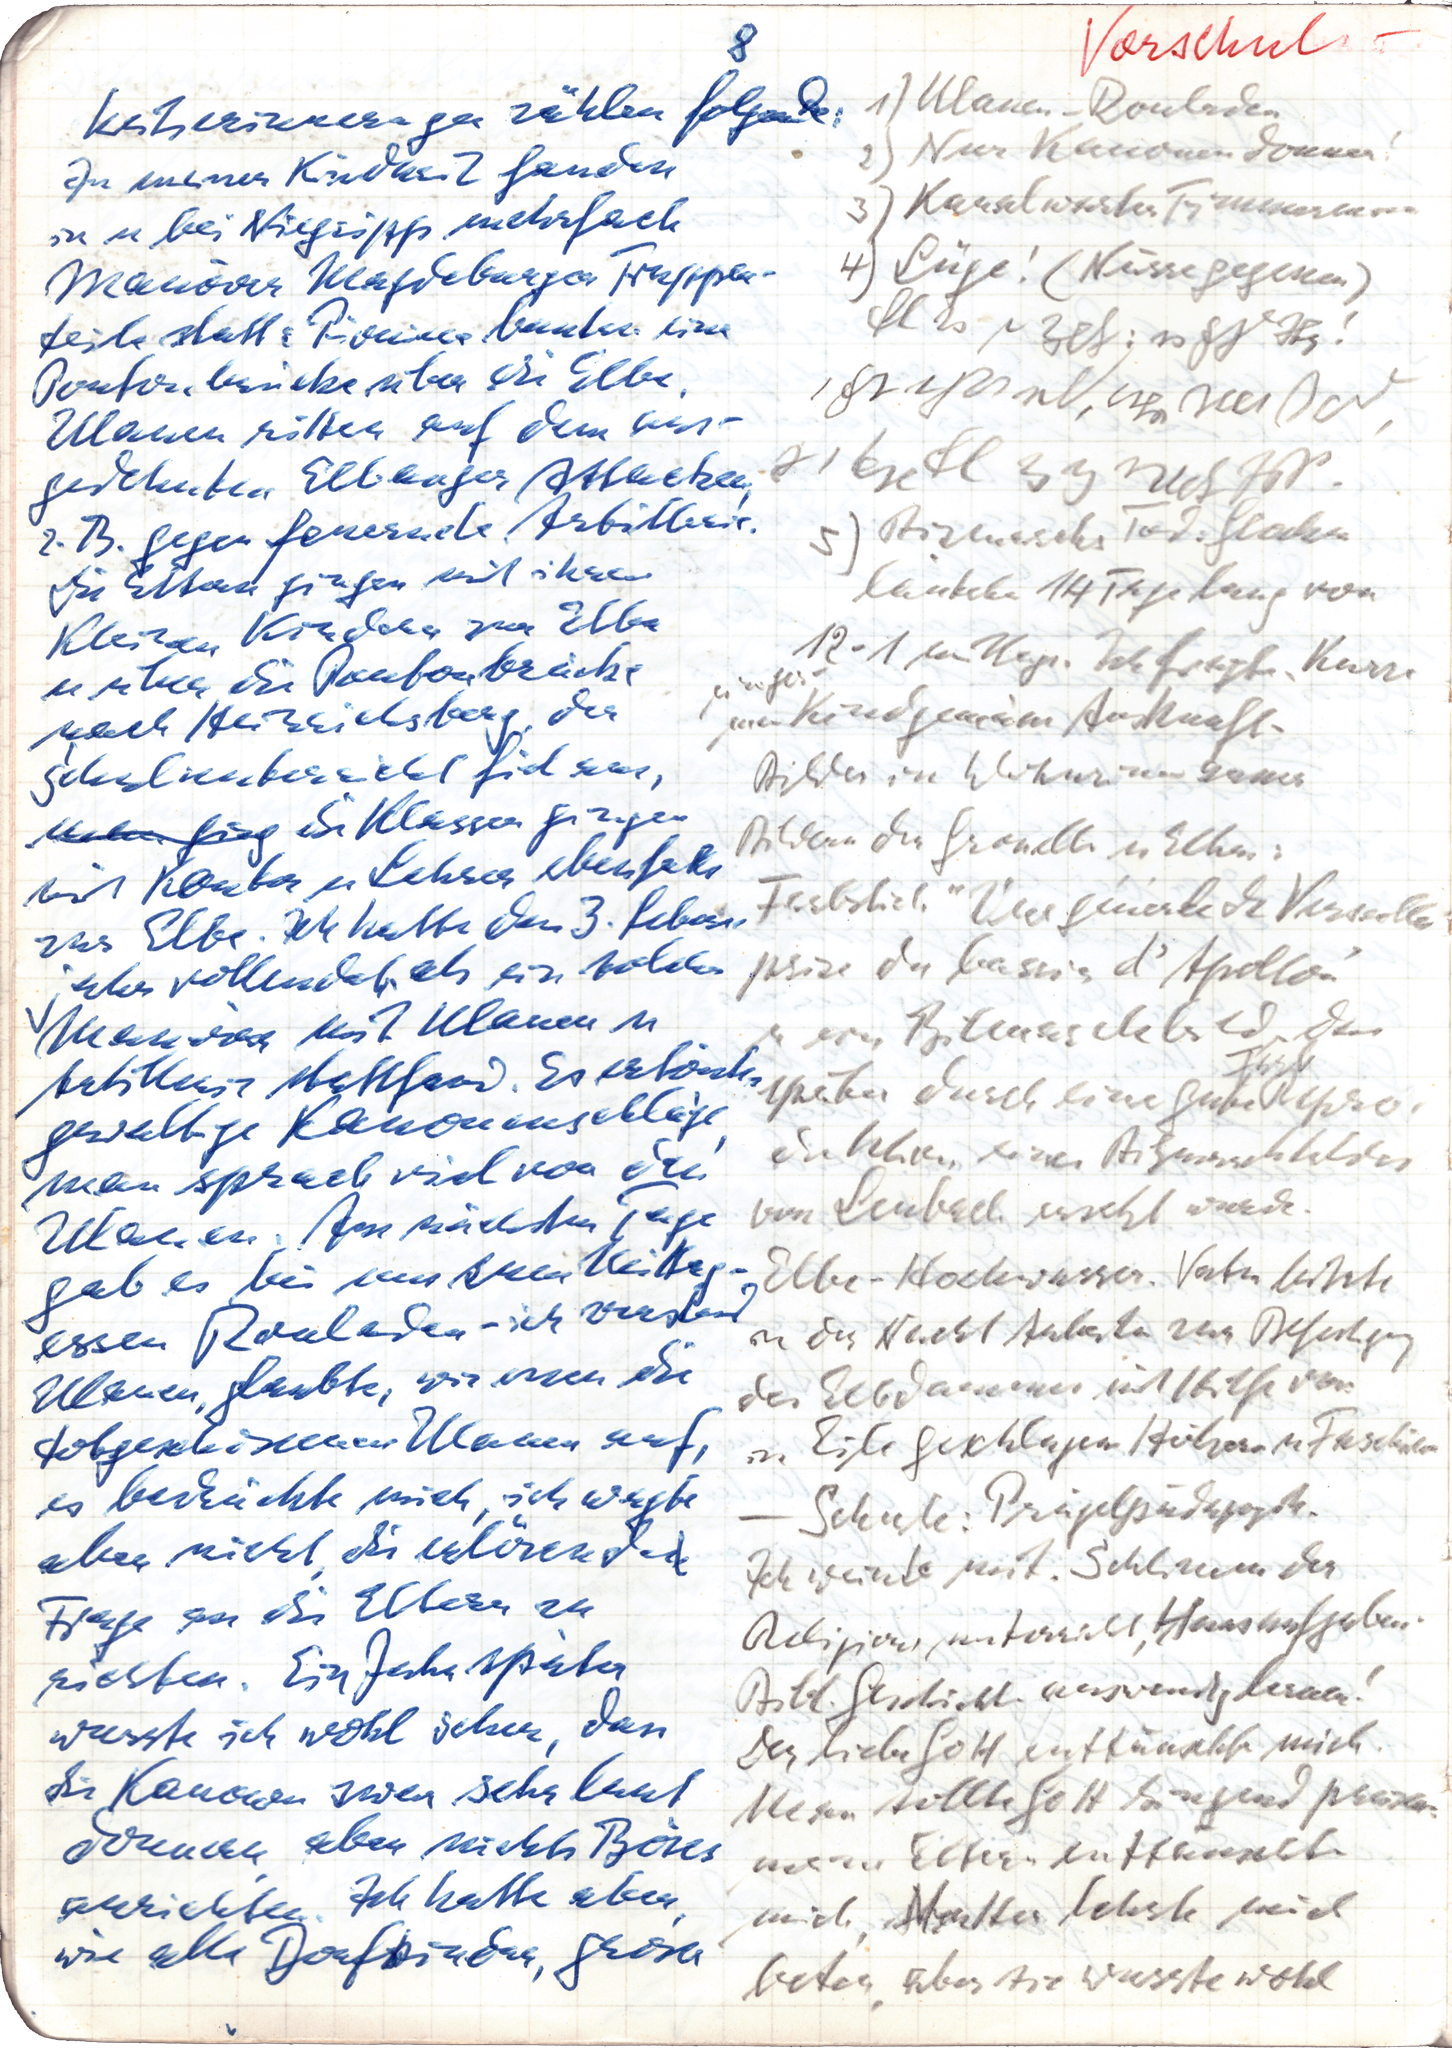
\includegraphics[width=\linewidth]{Photos/Doppelseite-links.png}
	\caption{Beispielseite, links}
	\label{fig:doppelseite_links}
\end{figure}

\begin{figure}[p]
	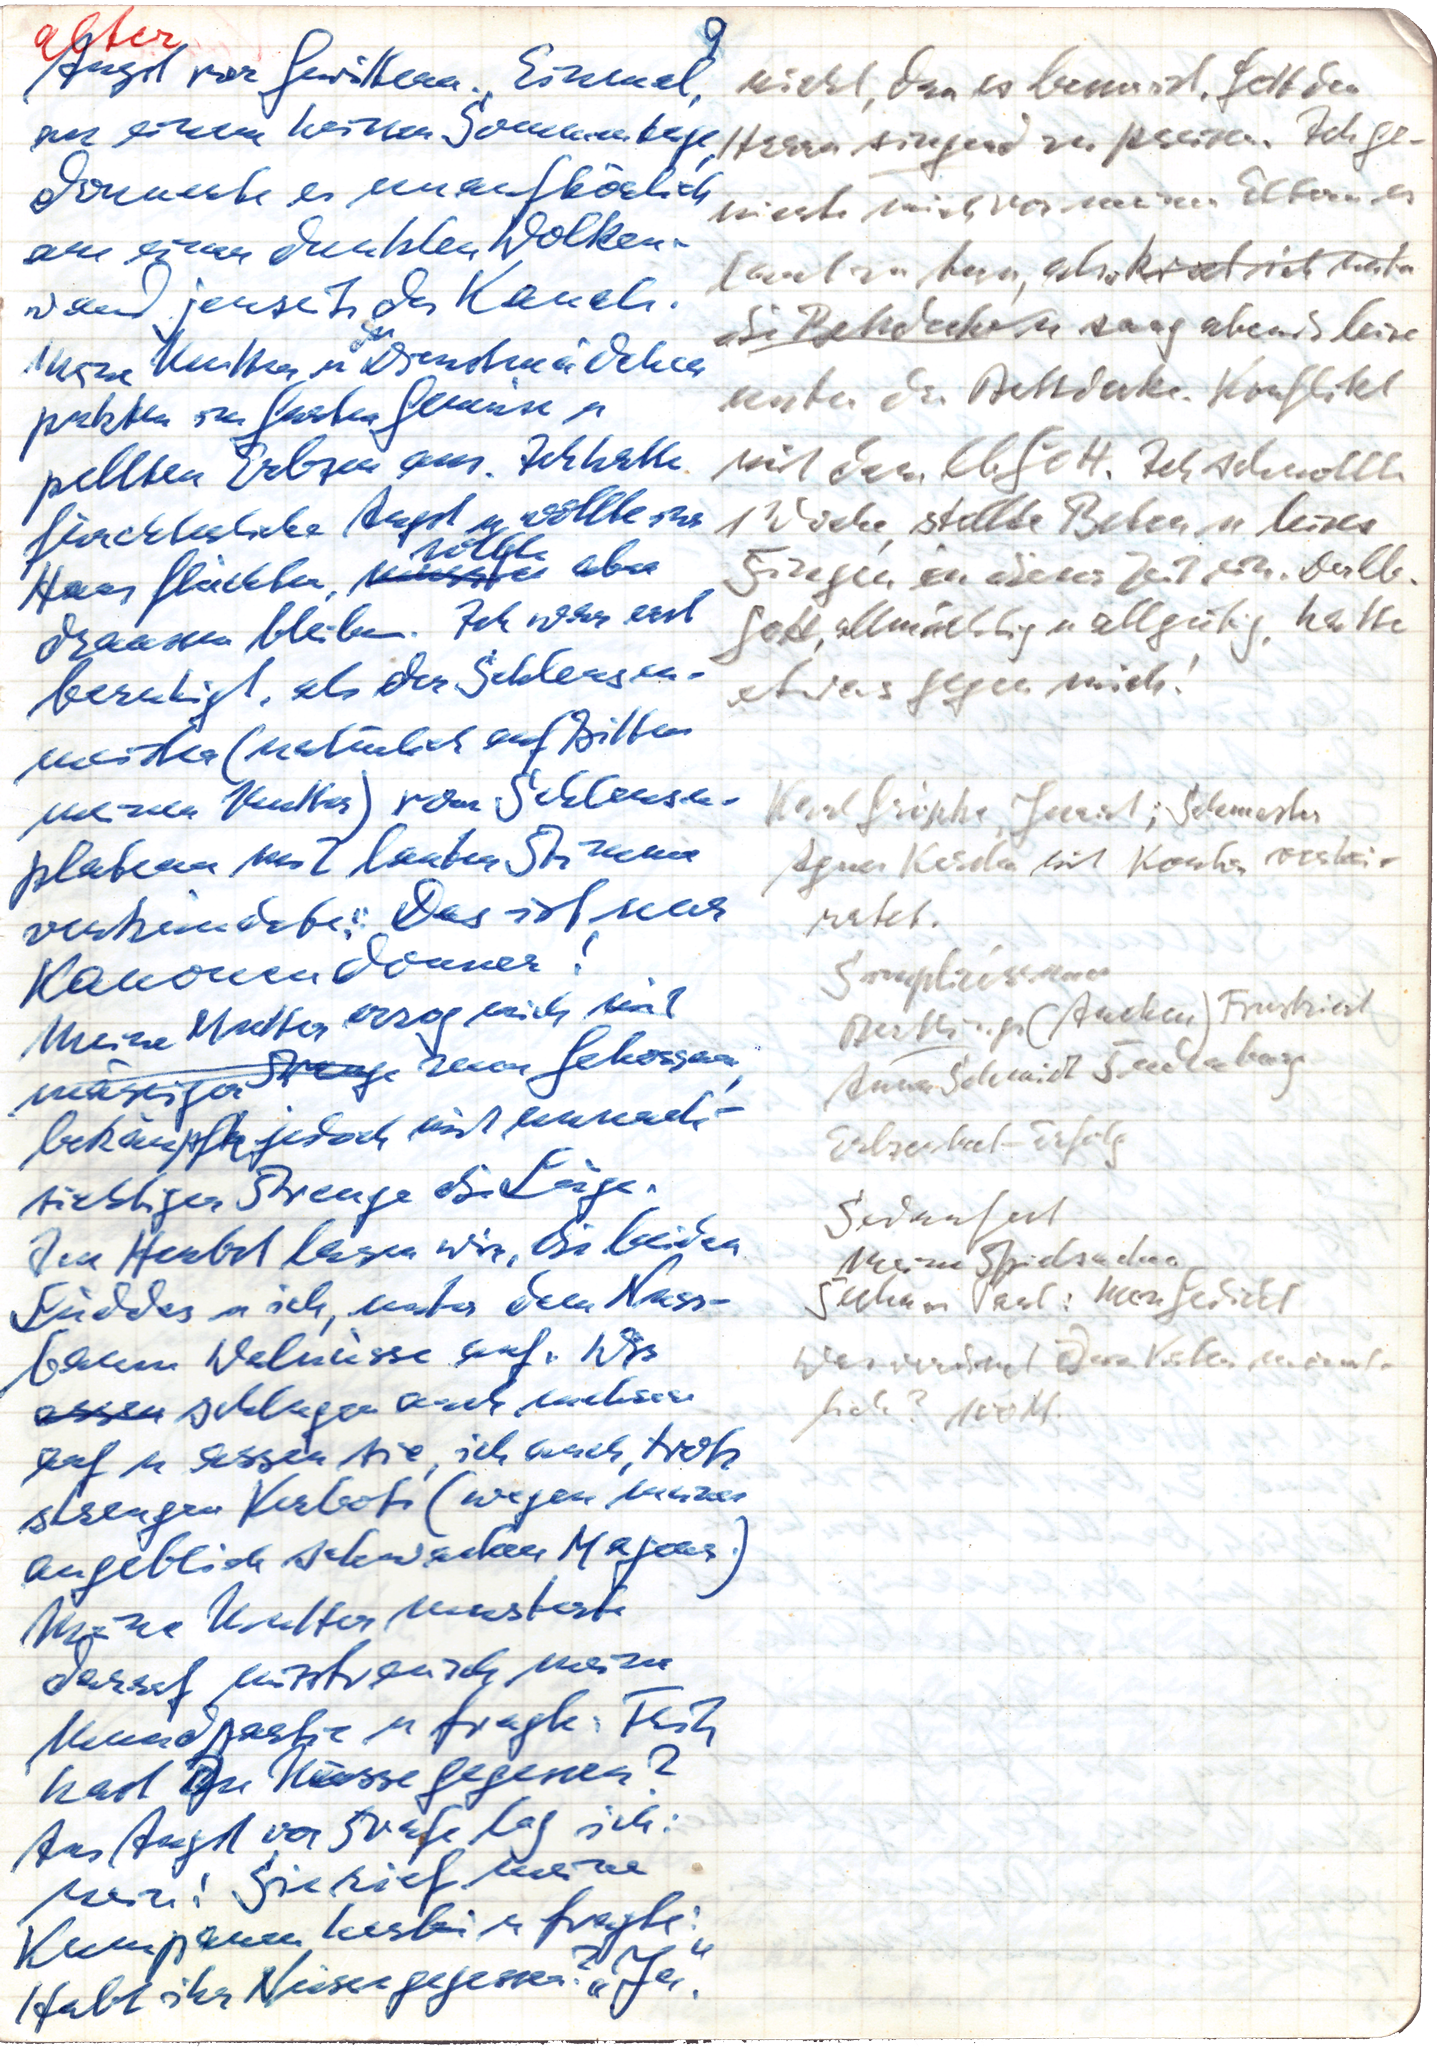
\includegraphics[width=\linewidth]{Photos/Doppelseite-rechts.png}
	\caption{Beispielseite, rechts}
	\label{fig:doppelseite_rechts}
\end{figure}

Nach Erinnerung von Helga hat Fritz seine Ideen und Formulierungen häufig Margot vorgetragen, die dann ihrerseits Anregungen gab und Anmerkungen machte. Dies fand zum großen Teil auch während der Aufenthalte in Barnave statt, wo Fritz und Margot häufig den Sommer verbrachten (manchmal schon ab Mai und bis in den September!).\\

Die Aufzeichnungen von Fritz befinden sich in 7 DIN-A5-Oktavheften mit dem Titel \enquote{Meine Lebenserinnerungen im Abriss} auf insgesamt 707 Seiten. Mit blauem Kugelschreiber hat Fritz in sehr enger und kleiner Schrift chronologisch geordnet seine Lebenserinnerungen aufgezeichnet. Vermutlich hat er in mehreren Heften gleichzeitig geschrieben: das Oktavheft, das mit seiner Kindheit beginnt, ähnelt äußerlich dem Oktavheft, das die Ereignisse ab März 1945 beschreibt, auch beginnt er in beiden Heften mit der Seitenzahl \enquote{1}. Die Seitenzahlen in den übrigen Heften führen die Nummerierung des jeweils vorigen Heftes fort.

Für die Aufzeichnungen hat Fritz die Seiten immer in der Hälfte gefaltet und zunächst nur den linken Teil beschrieben. Der rechte Teil war freigelassen für Verbesserungen und Ergänzungen, die ihm später eingefallen sind. Im ersten Oktavheft hat er zu Beginn mit rotem Kugelschreiber den Doppelseiten eine \enquote{Überschrift} gegeben. Da dies jedoch keine 10 Seiten durchgehalten wurde, hat Konstantin eine eigene Gliederung für die Aufzeichnungen erstellt. In den letzten beiden Heften von Fritz ist seine Schrift deutlich kleiner als in den vorherigen Heften, deswegen war zum Entziffern häufig eine Lupe notwendig. Vereinzelt enthalten die Hefte Notizen aus seinem Alltag (z.B. Personen- oder Buchnamen sowie zu klärende Fragen), oft schwer lesbar oder sogar in Stenographie. Sie werden hier nicht wiedergegeben, da sie offenkundig keine relevanten Informationen enthalten. Die Abbildungen \ref{fig:doppelseite_links} und \ref{fig:doppelseite_rechts} vermitteln einen Eindruck der Oktavhefte (Transskription siehe S. \pageref{para:kindheitserinnerungen}).\\

Die Tagebücher wurden von Helga handschriftlich in 3 große DIN-A4-Hefte übertragen. Orts- und Eigennamen wurden soweit möglich plausibilisiert und ggf. korrigiert. Fritz hat grundsätzlich kein \enquote{ß} benutzt, sondern immer \enquote{ss} geschrieben. Dies wurde an die aktuelle Rechtschreibung angepasst, um die Leserlichkeit zu verbessern. Ergänzungen sowie bei kyrillischen Wörtern die Transliteration sind in eckigen Klammern gesetzt, Erläuterungen oder Erinnerungen von Helga wurden als Fußnoten eingefügt.

Den Großteil der Abschrift machte Helga von Juli 1997 bis 2002 während der Sommerferien in Barnave, den Teil ab März 1945 (d.h. Kapitulation, Flucht aus Breslau und das Leben in Magdeburg) im Frühjahr 2021. Konstantin begann mit der Übertragung nach \LaTeX während des Lockdown-Weihnachten 2020 und vollendete sie im \enquote{Corona-Exil} in Berlin im Mai 2021.\\



\rightline{Konstantin Gründger} \leavevmode \\


\newpage
\appendix
\addchap{Anhang}
\section*{Abkürzungen}
\begin{acronym}
	\acro{eki}[EK I]{Eisernes Kreuz I. Klasse}
	\acro{ekii}[EK II]{Eisernes Kreuz II. Klasse}
	\acro{nsdap}[NSDAP]{Nationalsozialistische Deutsche Arbeiterpartei}
	\acro{oschrat}[OSchRat]{Oberschulrat}
	\acro{ostd}[OStD]{Ober\-studien\-di\-rek\-tor}
	\acro{ostr}[OStR]{Oberstudienrat}
	\acro{pg}[PG]{Parteigenosse}
	\acro{vg}[VG]{Volksgenosse}
	\acro{psk}[PSK]{Provinzialschulkollegium}
\end{acronym}

\newpage
\section*{Tabellen}
\begin{table}[h!]
	\label{tab:jahrgangsstufen}
	\centering
	\begin{tabular}{l|l||l}
		damals & Abk. & heute \\
		\hline
		Sexta & VI & Klasse 5 \\
		Quinta & V & Klasse 6 \\
		Quarta & IV & Klasse 7 \\
		Untertertia & U III & Klasse 8 \\
		Obertertia & O III & Klasse 9 \\
		Untersekunda & U II & Klasse 10 \\
		Obersekunda & O II & Klasse 11 \\
		Unterprima & U I & Klasse 12 \\
		Oberprima & O I & Klasse 13 \\
	\end{tabular}
	\caption{Jahrgangsstufen damals und heute}
\end{table}

\begin{table}[h!]
	\label{tab:lebensmittelkarten}
	\centering	
	\begin{tabular}{l|l}
		Kategorie & Personengruppe \\
		\hline
		I & Schwerstarbeiter und Funktionäre \\
		II & Schwerarbeiter \\
		III & Arbeiter \\
		IV & Angestellte \\
		V & Sonstige (Kinder, Rentner, NSDAP-Mitglieder, \\
		& Schwerbehinderte, Nichterwerbstätige), auch \enquote{Friedhofskarte}\\
		& genannt (die Zuteilung war praktisch \enquote{Null})
	\end{tabular}
	\caption{Lebensmittelkarten in der Sowjetischen Besatzungszone\\ ab 12. Juni 1945}
\end{table}

\end{document}



